% concatenated from afio.tex, mydefs.tex, cutoffFig.tex, parametrix.tex, applicshort.tex, raypic.tex, appendix.tex
\documentclass[
	fontsize=11pt, 
	twoside=false, 
	abstract=true, 
	a4paper,
]{scrartcl}
 
\usepackage[bookmarkdepth=subsection,font=bembo]{templ}

\usepackage{bm}
\usepackage{mathrsfs}

\usepackage{tikz}
\usetikzlibrary{arrows}
\usetikzlibrary{positioning}
\usetikzlibrary{shapes.geometric}
%\usepackage{calc}
\usepackage{pgf}
\usetikzlibrary{patterns}
\usetikzlibrary{patterns.meta}
%\usepgflibrary{plothandlers} % LaTeX and plain TeX and pure pgf
%\usepgflibrary[plothandlers] % ConTeXt and pure pgf
%\usetikzlibrary{plothandlers} % LaTeX and plain TeX when using TikZ
%\usetikzlibrary[plothandlers] % ConTeXt when using TikZ
\usetikzlibrary{topaths} % LaTeX and plain TeX
\usetikzlibrary[topaths] % ConTeXt
\usetikzlibrary{decorations.markings}

\makeatletter
\newcommand{\leqnomode}{\tagsleft@true\let\veqno\@@leqno}
\newcommand{\reqnomode}{\tagsleft@false\let\veqno\@@eqno}
\makeatother
\newcommand{\eps}{\varepsilon}
\newcommand{\sem}{\setminus\{0\}}
\newcommand{\RR}{\mathbb{R}}
\newcommand{\mr}[1]{\mathring{#1}}
\newcommand{\CC}{\mathbb{C}}
\newcommand{\DD}{\mathscr{D}}
\newcommand{\Ss}{\mathscr{S}}
\newcommand{\EE}{\mathscr{E}}
\newcommand{\dd}{\mathrm{d}}
\newcommand{\Fou}[1]{\mathscr{F}\left(#1\right)}
\newcommand{\FouI}[1]{\mathscr{F}^{-1}\left(#1\right)}
\newcommand{\CcRn}{C_c^\infty(\RR^{N'})}
\newcommand{\Cc}[1]{C_c^\infty\left(#1\right)}
\newcommand{\norm}[1]{\left\lVert#1\right\rVert}
\newcommand{\abs}[1]{\left\lvert#1\right\rvert}
\newcommand{\del}{\partial}
\newcommand{\supp}{\mathrm{supp}}
\newcommand{\LL}{\mathcal{L}}
\newcommand{\Char}[1]{\mathrm{Char}\left(#1\right)}
\newcommand{\ess}[1]{\mathrm{esssupp}\left(#1\right)}
\newcommand{\comp}{\mathcal{c}}
\newcommand{\ssupp}{\mathrm{sing}\,\mathrm{supp}}
\newcommand{\td}[1]{\tilde{#1}}
\newcommand{\an}{\quad\text{and}\quad}
\newcommand{\dist}{\mathrm{dist}}
\newcommand{\id}{\mathrm{id}}
\newcommand{\wf}{\mathrm{WF}_{\mathrm{a}}}
\newcommand{\es}{\mathrm{ess}\ \mathrm{supp}}
\newcommand{\ud}[1]{\underline{#1}}
\newcommand{\neu}[1]{\del_{x_n}#1\bigr|_{\{x_n=0\}}}
\newcommand{\tdo}{\tilde{\Omega}}
\newcommand{\itdo}{1_{\tilde{\Omega}}}
\newcommand{\bdry}{(h\td{\del}_\nu+(\td{\del}_\nu\phi))}
\newcommand{\mf}[1]{\oldmathbb{#1}}
\newcommand{\bsc}[1]{\textbf{\ebgaramond\textsc{#1}}}
\newcommand{\sisu}{\mathrm{sing}\ \mathrm{supp}}

\usepackage{xparse}

\NewDocumentCommand{\op}{O{h}m}{\mathrm{Op}_{#1}\left(#2\right)}
\NewDocumentCommand{\tbdry}{O{}}{\tau_{#1}\bdry}



\addbibresource{library.bib} 

\begin{document} 

\title{Analytic Fourier Integral Operators and a Problem from Seismic Inversion}

\author{Leonard Busch$^{1}${\href{mailto:l.a.busch@uva.nl}{\color{blue}\Letter}}}%\and Leo Tzou$^{2}${\href{mailto:leo.tzou@unimelb.edu.au}{\color{blue}\Letter}}}

\date{\footnotesize$^1$Korteweg-de Vries Institute for Mathematics, University of Amsterdam, Amsterdam, The Netherlands}%\\\footnotesize$^2$University of Melbourne, Australia}

\maketitle

\vspace{-2.5\baselineskip}
\begin{abstract}
\noindent
We establish a general result about the recovery of the analytic wavefront set of a distribution from the analytic wavefront set of its transform coming from a classical elliptic analytic Fourier integral operator (FIO) satisfying some conditions including the Bolker condition. Furthermore, we give a simple explicit analytic parametrix in the form of a classical elliptic analytic FIO for general analytic second order hyperbolic differential operators. Finally, we apply these results together with microlocal analytic continuation and a layer stripping argument to a problem from seismic inversion to prove the injectivity of a linearized operator in the analytic setting.

It is the use of wave packet techniques that allows us to %account for every single analytic singularity and precisely 
give the precise relation how the FIOs under consideration transform the analytic wavefront set, whereas the explicit analytic parametrix comes from a reformulation of the parametrix construction of Hadamard and H\"ormander.
%This significantly generalizes the set of analytic FIO for which one can resolve the analytic wavefront set, for example paving the way for parametrices of strictly hyperbolic differential operators. 

	\emptyfootnote{\noindent\emph{2020 Mathematics Subject Classification:} Primary: 35S30, 35A18, 35A20. Secondary: 35L05, 42B10.}
	\emptyfootnote{\noindent\emph{Key words and phrases:} Analytic Fourier integral operator, FBI transform, wave packet decomposition, analytic wavefront set, Bolker condition, inverse problem, acoustic wave equation}
	%\emptyfootnote{\noindent*Corresponding author: Leonard Busch}
\end{abstract}

%{\hypersetup{linkcolor=black}\tableofcontents}

%Put
%\begin{equation}
%    C \subset T^\ast \mathcal{G} \times T^\ast M^{\mathrm{int}}
%\end{equation}
%and 
%\begin{equation}
%    \pi_L \colon C \to T^\ast\mathcal{G}\setminus\{0\}\,,\an \pi_R \colon C \to T^\ast M^{\mathrm{int}}\setminus\{0\}
%\end{equation}
%Take 
%\begin{equation}
%    n = n'+n'', N \geq n, \phi \colon \RR^N\times \RR^{n'} \to \RR^{n''}, \Phi\colon \RR^{N+n+n''}\to \RR\,, \quad \Phi(z,x,\eta) = (\phi(z,x')-x'')\cdot \eta\,.
%\end{equation}
%
%For $V,U'$ neighborhoods around $\hat z,\hat x'$ we have 
%\begin{equation}
%	C = \{(z,\nabla_z \Phi(z,x,\eta);x,\nabla_x\Phi(z,x,\eta))\colon \nabla_\eta\Phi(z,x,\eta)=0\,,z\in V\,,x'\in U'\}\,.
%\end{equation}
%
%Put $\mathcal{V} = \pi_L{\td{C}}$ where $\td{C}\subset C$ and define 
%\begin{equation}
%	\chi\coloneqq \pi_R \circ \pi_L^{-1} \colon \mathcal{V} \to \pi_R(C) \subset T^\ast U\,,
%\end{equation}
%and $\chi$ is analytic on $\mathcal{V}$. Thus
%\begin{equation}
%	\chi(z,\xi) = (x,\omega) \iff \begin{cases}
%		\xi &= \nabla_z \Phi(z,x,\eta)\,,\\
%		\omega &= \nabla_x\Phi(z,x,\eta)\,,\\
%		x''&=\varphi(z,x') \iff \nabla_\eta \Phi(z,x,\eta) =0\,,\\
%		x' &\in U'
%	\end{cases} 
%\end{equation}
%
%Now fix $g_n \in S^{1/2}_{1/2}(\RR^{N'}), g_N \in S^{1/2}_{1/2}(\RR^N)$ and take $(u_1,u_2)= u\in\RR^{2n},(v_1,v_2)=v\in\RR^{2N}$ and put 
%\begin{equation}
%	g_{n,u} = e^{iu_2\cdot}g_n(\cdot-u_1)\,,\an g_{N,v}=e^{iv_2\cdot}g_N(\cdot-v_1)\,.
%\end{equation}
%We are given the kernel 
%\begin{equation}
%	T(z,x) = \int_{\RR^{n''}}e^{i\Phi(z,x,\eta)}a(z,x)\dd\eta\,.
%\end{equation}
%and also denote its operator by $T$.
%
%Then 
%\begin{align*}
%	\langle Tg_{n,u},g_{N,v}\rangle &= \int_{\RR^{N+n+n''}}e^{iu_2\cdot x}g_n(x-u_1)e^{i\Phi(z,x,\eta)}a(z,x)e^{-iv_2\cdot z}\bar g_{N}(z-v_1)\dd\eta\dd x\dd z \\
%	&= \int_{\RR^{N+n+n''}}e^{i\left(\Phi(z+v_1,x+u_1,\eta)+u_2\cdot(x+u_1)-v_2\cdot(z+v_1)\right)}a(z+v_1,x+u_1)g_n(x)\bar g_N(z) \dd\eta\dd x\dd z\,.
%\end{align*}
%
%Let 
%\begin{equation}\label{eq:epschi}
%	\varepsilon_\chi = \abs{\chi(v)-u} > 0
%\end{equation}
%
%
%\begin{lemma}
%	There is a constant $C>0$ so that if $\norm{\eta-\eta(v)} < C$, then 
%	\begin{equation}
%		\abs{\chi(v)-(u_1,-u_2)} \lesssim \abs{\nabla_{(z,x)}\Phi(v_1,u_1,\eta)+(-v_2,u_2)} 
%	\end{equation}
%\end{lemma}
%\begin{proof}
%
%	Note that $v_2 = \nabla_z\Phi(v_1,x(v),\eta(v))$.
%
%	\begin{align*}
%		\abs{u_1-x(v)} &\leq \abs{\begin{pmatrix}u_1-x(v)\\\nabla_x\Phi(v_1,u_1,\eta(v))-\nabla_x\Phi(v_1,x(v),\eta(v))\end{pmatrix}} \\
%		&= \abs{\chi(v_1,\nabla_z\Phi(v_1,u_1,\eta(v)))-\chi(v_1,\nabla_z\Phi(v_1,x(v),\eta(v)))} \\
%		&\leq C_{\chi}\abs{\begin{pmatrix}v_1 - v_1\\\nabla_z\Phi(v_1,u_1,\eta(v))-\nabla_z\Phi(v_1,x(v),\eta(v))\end{pmatrix}} \\
%		&\leq C_{\chi}\abs{\nabla_z\Phi(v_1,u_1,\eta)-\nabla_z\Phi(v_1,x(v),\eta(v))}+C_{\chi}\abs{\nabla_z\Phi(v_1,u_1,\eta(v))-\nabla_z\Phi(v_1,u_1,\eta)} \\
%		&\leq C_{\chi}\abs{\nabla_z\Phi(v_1,u_1,\eta)-v_2}+C_{\chi}C_{\Phi_z,\eta}\abs{\eta(v)-\eta}\,.
%	\end{align*}
%	For the second step we do as follows: notice that $\omega(v)=\nabla_x\Phi(v_1,x(v),\eta(v))$
%	\begin{align*}
%		\abs{\omega(v)+u_2} &= \abs{\nabla_x\Phi(v_1,x(v),\eta(v)) -\nabla_x\Phi(v_1,u_1,\eta(v))+\nabla_x\Phi(v_1,u_1,\eta(v))-\nabla_x\Phi(v_1,u_1,\eta)+\nabla_x\Phi(v_1,u_1,\eta)+u_2}\\
%		&\leq \abs{\nabla_x\Phi(v_1,x(v),\eta(v)) -\nabla_x\Phi(v_1,u_1,\eta(v))} + \abs{\nabla_x\Phi(v_1,u_1,\eta(v))-\nabla_x\Phi(v_1,u_1,\eta)} + \abs{\nabla_x\Phi(v_1,u_1,\eta)+u_2} \\
%		&\leq C_{\Phi_x,x}\abs{u_1-x(v)} + C_{\Phi_x,\eta}\abs{\eta-\eta(v)}+\abs{\nabla_x\Phi(v_1,u_1,\eta)+u_2}
%	\end{align*}
%	Now we note that 
%	\begin{align*}
%		\abs{\chi(v)-(u_1,-u_2)} &\leq \abs{x(v)-u_1} + \abs{\omega(v)+u_2} \\
%		&\leq \abs{\nabla_x\Phi(v_1,u_1,\eta)+u_2} + \abs{\eta-\eta(v)}(C_{\Phi_x,\eta}+C_\chi C_{\Phi_z,\eta}(1+C_{\Phi_x,x})) \\
%		&+ (1+C_{\Phi_x,x})C_\chi \abs{\nabla_z\Phi(v_1,u_1,\eta)-v_2}
%	\end{align*}
%	and because $a+b \leq 2\sqrt{a^2+b^2}$ for $a,b\geq 0$, and put $C' = (C_{\Phi_x,\eta}+C_\chi C_{\Phi_z,\eta}(1+C_{\Phi_x,x}))$ and $C'' = (2(1+C_{\Phi_x,x})C_\chi)^{-1}$ or so,
%	\begin{align*}
%		\abs{\nabla_{(z,x)}\Phi(v_1,u_1,\eta)+(-v_2,u_2)} \geq C'' \abs{\chi(v)-(u_1,-u_2)} - C'\abs{\eta-\eta(v)}
%	\end{align*}
%	so that if $\abs{\eta-\eta(v)} \leq \varepsilon_\chi (C'')^{-1}(C')^{-1}/2$, with $\varepsilon_\eta < 1$ then 
%	\begin{equation}
%		\abs{\nabla_{(z,x)}\Phi(v_1,u_1,\eta)+(-v_2,u_2)} \geq C''/2\abs{\chi(v)-(u_1,-u_2)}
%	\end{equation}
%	which concludes the proof.
%\end{proof}
%
%We now split up the expression with $G(z,x) = g_n(x)\bar g_N(z)$ 
%\begin{equation}
%	\langle Tg_{n,u},g_{N,v}\rangle = I+II 
%\end{equation}
%with 
%\begin{align*}
%	I &= \int_{\RR^{n+n''}} \int_{\abs{\eta-\eta(v)< C}}e^{i\left(\Phi(z+v_1,x+u_1,\eta)+u_2\cdot(x+u_1)-v_2\cdot(z+v_1)\right)}a(z+v_1,x+u_1)G(z,x) \dd\eta\dd x\dd z\,. \\
%	II &= \int_{\RR^{n+n''}} \int_{\abs{\eta-\eta(v)\geq C}}e^{i\left(\Phi(z+v_1,x+u_1,\eta)+u_2\cdot(x+u_1)-v_2\cdot(z+v_1)\right)}a(z+v_1,x+u_1)G(z,x) \dd\eta\dd x\dd z\,.
%\end{align*}
%
%We deal with $I$ as follows: by Taylor:
%\[
%	\Phi(z+v_1,z+u_1,\eta) = \Phi(v_1,u_1,\eta)+\nabla_{(z,x)}\Phi(v_1,u_1,\eta)\cdot (z,x) + \Phi_{2,(v_1,u_1)}(z,x,\eta)	
%\]
%with 
%\[
%	\abs{\del^{\alpha}_{(z,x)}\Phi_{2,(v_1,u_1)(z,x)}} \leq C^{\abs{\alpha}}(\alpha!)\langle (z,x)\rangle^2\,.
%\]
%So that for $I$ we see:
%\begin{align*}
%	\abs{I} &\leq \int_{\RR^{n+n''}} \int_{\abs{\eta-\eta(v)< C}}\abs{e^{i(\Phi(v_1,u_1,\eta)+u_2\cdot u_1 - v_2\cdot v_1)}}e^{i\left((\nabla_{(z,x)}\Phi(v_1,u_1,\eta)-(v_2,-u_2))\cdot (z,x) + \Phi_{2,(v_1,u_1)}(z,x,\eta)\right)}a(z+v_1,x+u_1)G(z,x) \dd\eta\dd x\dd z
%\end{align*}
%
%So it is sufficient to show that $\abs{I} \leq \exp(-\varepsilon\abs{\nabla_{(z,x)}\Phi(v_1,u_1,\eta)-(v_2,-u_2)})$, so that if we put 
%\[
%	I_{0,v_1,v_2,\eta}(\zeta) =  \int_{\RR^{n+n''}} e^{i\Phi_{2,(v_1,u_1)}(z,x,\eta)} e^{i\zeta \cdot (z,x)}a(z+v_1,x+u_1)G(z,x)\dd x\dd z
%\]
%that 
%\[
%	\abs{\zeta^\alpha I_{0,v_1,v_2}(\zeta)} \lesssim C^{\abs{\alpha}}\alpha!\,.	
%\]
%then 
%\[
%	\abs{I} \leq \int_{\abs{\eta-\eta(v)}<C} I_{0,v_1,u_1,\eta}(\nabla_{(z,x)}\Phi(v_1,u_1,\eta)-(v_2,-u_2)) \dd\eta \leq m(B_C(0)) \exp(-\varepsilon \abs{\chi(v)-u})\,. 	
%\]
%
%To deal with $II$ we proceed as follows: due to linearity:
%\[
%	\Phi(z+v_1,x+u_1,\eta) = \Phi(z+v_1,x+u_1,\eta(v)) + \Phi(z+v_1,x+u_1,\eta-\eta(v))
%\]
%then 
%\begin{align*}
%	\abs{II} \leq \int_{\RR^{n'+n''}} \abs{e^{i(\Phi(z+v_1,x+u_1,\eta(v))+u_2\cdot x - v_2 \cdot z)} \int_{\abs{\eta-\eta(v)}\geq C} e^{i\Phi(z+v_1,x+u_1,\eta-\eta(v))} a(z+v_1,x+u_1)G(z,x)\dd\eta} \dd x\dd z
%\end{align*}
%
%Now note that 
%\[ 
%	\frac{(\eta-\eta(v))\cdot \nabla_{x''}}{i\abs{\eta-\eta(v)}^2}e^{i\Phi(z+v_1,x+u_1,\eta-\eta(v))} = e^{i\Phi(z+v_1,x+u_1,\eta-\eta(v))}\,.
%\]
%
%\hrule
%
%\quad
%
%If we do the full case: the part with $II$ should still work I think.
%
%
%Let $\Omega_j \subset \RR^{n_j}$ open subsets and $\Theta \subset \RR^N\setminus\{0\}$ be open cone, $\varphi \in C^\infty(\Omega_1\times\Omega_2\times \Theta)$,
%\begin{equation}
%	\Gamma_\varphi = \{(x,y,\eta) \in \Omega_1\times\Omega_2\times\Theta\colon \del_\eta\varphi(x,y,\eta)=0\}.
%\end{equation}
%$\varphi$ phase function, so real-valued, homogenous of degree one, and
%\begin{enumerate}
%	\item $\Gamma_\varphi$ is closed conic $C^\infty$ submanifold of $\Omega_1\times\Omega_2\times\Theta$,
%	\item the rank of the map $(p_\varphi,q_\varphi)(x,y,\eta) = (x,\varphi_x(x,y,\eta),y,-\varphi_y(x,y,\eta))$ is $n_1+n_2$ at every point in $\Gamma_\varphi$
%	\item $\forall (x,y,\eta)\in \Gamma_\varphi$ we have $\varphi_x$ or $\varphi_y$ $\neq 0$
%\end{enumerate}
%
%Put  
%\begin{equation}
%	\Lambda_\varphi = (p_\varphi,q_\varphi)(\Gamma_\varphi) = \{(x,\varphi_x(x,y,\eta),y,-\varphi_y(x,y,\eta)) \colon \varphi_\eta(x,y,\eta) = 0\}\,.
%\end{equation}
%Now for $a\in S^m(\Omega_1\times\Omega_2,\Theta)$ where we may assume that $m<-N$. If this were not the case, we could proceed as in \cite[Thm.~18.1.13]{MR4436039} to get to this case using limits I think. 
%
%define the kernel $K(x,y)$ as 
%\begin{equation}
%	K(x,y) = (2\pi)^{-N}\int_\Theta e^{i\varphi(x,y,\eta)}a(x,y,\eta)\dd\eta
%\end{equation}
%and let $g_i \in S^{1/2}_{1/2}(\RR^{n_i})$, $u = (u_+,u_-) \in \RR^{2n_1}$, $v = (v_+,v_-) \in \RR^{2n_2}$ and put 
%\[
%	g_{1,u}(x) = e^{iu_-x}g_1(x-u_+)\,,\an g_{2,v}(y) = e^{iv_-y}g_2(y-v_+)\,.
%\]
%Then 
%\[
%	\langle K g_{2,v},g_{1,u} \rangle = (2\pi)^{-N} \int_{\Omega_1\times\Omega_2\times\Theta} e^{i(\varphi(x+u_+,y+v_+,\eta)+v_-\cdot(y+v_+)-u_-\cdot(x+u_+))}a(x+u_+,y+v_+,\eta)G(x,y)\dd\eta\dd y \dd x\,,	
%\]
%where $G(x,y) = g_2(y)\bar g_1(x)$. 
%
%Let $u,v$ be fixed. We define the set 
%\[
%	A = A_{u,v} = \{\eta\in\Theta \colon (u_+,\varphi_x(u_+,v_+,\eta), v_+,-\varphi_y(u_+,v_+,\eta)) \in \Lambda_\varphi\}\,.	
%\]
%
%Using Taylor we have that 
%\begin{align*}
%	&{}\varphi(x+u_+,y+v_+,\eta)+v_-\cdot(y+v_+)-u_-\cdot(x+u_+) \\
%	&= \left(\varphi(u_+,v_+,\eta) + v_+\cdot v_- - u_-\cdot u_+\right) + \left(\varphi_{(x,y)}(u_+,v_+,\eta)-(u_-,-v_-)^T\right)\cdot (x,y)^T + \varphi_{2,u_+,v_+}(x,y,\eta)\,, 	
%\end{align*}
%where $\varphi_{2,u_+,v_+}$ is the remainder term and we'll deal with that some other time. The first term only depends on $\eta$ and so it'll disappear as in the exponent if we just get the $\eta$ integral to be finite. 
%
%At the same time, due to the homogeneity of $\varphi:$
%\[
%	\eta\varphi_\eta(x,y,\eta) = \varphi(x,y,\eta)	
%\]
%and so $\varphi(x,y,\eta) = \varphi(x,y,\eta_0) + \varphi_\eta(x,y,\eta_0)\cdot(\eta-\eta_0) + \varphi_{3,\eta}$ where the last is a remainder term and cuz $\eta_0\cdot \varphi_\eta(\eta_0) = \varphi(\eta_0)$ we get 
%\[
%	\varphi(x,y,\eta) = \varphi(x,y,\eta_0)\cdot \eta + \varphi_{2,\eta}\,.	
%\]
%
%and so we could also write:
%\begin{align*}
%	&{}\varphi(x+u_+,y+v_+,\eta)+v_-\cdot(y+v_+)-u_-\cdot(x+u_+) \\
%	&= \left(\varphi(u_+,v_+,\eta) + v_+\cdot v_- - u_-\cdot u_+\right) + \left(\varphi_{(x,y,\eta)}(u_+,v_+,\eta_0)-(u_-,-v_-,0)^T\right)\cdot (x,y,\eta)^T + \varphi_{3,u_+,v_+}(x,y,\eta)\,, \\
%	&= \left(\varphi(u_+,v_+,\eta_0) + v_+\cdot v_- - u_-\cdot u_+\right) + \left(\varphi_{(x,y,\eta)}(u_+,v_+,\eta_0)-(u_-,-v_-,0)^T\right)\cdot (x,y,\eta-\eta_0)^T + \varphi_{4,u_+,v_+}(x,y,\eta)\,,
%\end{align*}
%for some new remainder thing $\varphi_{3,u_+,v_+}$.
%
%Now we distinguish between two cases: $A =\emptyset$ and $A\neq\emptyset$.
%
%We assume that $\delta = \dist(\Lambda_\varphi, (u,v)^T) >0$
%
%\subsection{The case $A \neq \emptyset$}
%
%We have that 
%\begin{align*}
%	\dist(\Lambda_\varphi, (u,v)^T) &\leq \inf_{\eta_0\in A}\abs{\begin{pmatrix}u_+\\\varphi_x(u_+,v_+,\eta_0)\\v_+\\-\varphi_y(u_+,v_+,\eta_0) \end{pmatrix} - \begin{pmatrix}u_+\\u_-\\v_+\\v_-\end{pmatrix}} \\
%	&= \inf_{\eta_0\in A}\abs{\begin{pmatrix}\varphi_x(u_+,v_+,\eta_0)\\-\varphi_y(u_+,v_+,\eta_0) \end{pmatrix} - \begin{pmatrix}u_-\\-v_-\end{pmatrix}}
%\end{align*}
%
%Thus, for arbitrary $\eta\in\Theta$:
%\begin{align*}
%	\abs{\varphi_{(x,y)}(u_+,v_+,\eta)- (u_-,-v_-)^T} \geq \abs{\varphi_{(x,y)}(u_+,v_+,\eta_0)-(u_-,-v_-)^T}-\abs{\varphi_{(x,y)}(u_+,v_+,\eta_0)-\varphi_{(x,y)}(u_+,v_+,\eta)}
%\end{align*}
%Now if $\varphi_{(x,y)}$ is Lipschitz, we have that 
%\[
%	\abs{\varphi_{(x,y)}(u_+,v_+,\eta_0)-\varphi_{(x,y)}(u_+,v_+,\eta)} \leq L_1\abs{\eta_0-\eta}	
%\]
%for some Lipschitz constant $L_1$. 
%
%Thus, if $\abs{\eta_0-\eta} \leq (2L_1)^{-1}\delta$, then 
%
%\[
%	\abs{\varphi_{(x,y)}(u_+,v_+,\eta)- (u_-,-v_-)^T} \geq \delta(1-1/2) = 1/2 \delta\,,
%\]
%which is what we want. 
%
%Let's look at the case when $\abs{\eta_0-\eta} > (2L_1)^{-1}\delta$. 
%
%First notice that if $\eta = \lambda\eta_0$ for some $\lambda > 0$, then we could always choose $\eta_0$ so that $\eta = \eta_0$ and so their distance is small. 
%
%Thus for this case we may assume that $\eta$ and $\eta_0$ are not on the same ray. 
%
%\hrule 
%
%\quad
%
%other way: use full Taylor, then: 
%\begin{align*}
%	&{}\varphi(x+u_+,y+v_+,\eta)+v_-\cdot(y+v_+)-u_-\cdot(x+u_+) \\
%	&= \left(\varphi(u_+,v_+,\eta_0) + v_+\cdot v_- - u_-\cdot u_+\right) + \left(\varphi_{(x,y,\eta)}(u_+,v_+,\eta_0)-(u_-,-v_-,0)^T\right)\cdot (x,y,\eta-\eta_0)^T + \varphi_{4,u_+,v_+}(x,y,\eta)\,,
%\end{align*}
%and 
%We have that 
%\begin{align*}
%	\dist(\Lambda_\varphi, (u,v)^T) &\leq \inf_{\eta_0\in A}\abs{\begin{pmatrix}u_+\\\varphi_x(u_+,v_+,\eta_0)\\v_+\\-\varphi_y(u_+,v_+,\eta_0) \end{pmatrix} - \begin{pmatrix}u_+\\u_-\\v_+\\v_-\end{pmatrix}} \\
%	&= \inf_{\eta_0\in A}\abs{\begin{pmatrix}\varphi_x(u_+,v_+,\eta_0)\\-\varphi_y(u_+,v_+,\eta_0) \end{pmatrix} - \begin{pmatrix}u_-\\-v_-\end{pmatrix}}
%\end{align*}
%
%Thus,
%\begin{align*}
%	\abs{\varphi_{(x,y,\eta)}(u_+,v_+,\eta_0)- (u_-,-v_-,0)^T} \geq \abs{\varphi_{(x,y)}(u_+,v_+,\eta_0)-(u_-,-v_-)^T}
%\end{align*}
%and so
%\[
%	\abs{\varphi_{(x,y,\eta)}(u_+,v_+,\eta_0)- (u_-,-v_-)^T} \geq \delta
%\]
%which is what we want. 
%
%Then have
%\[
%	\langle K g_{2,v},g_{1,u} \rangle = (2\pi)^{-N} \int_{\Omega_1\times\Omega_2\times\Theta} e^{i(\varphi(x+u_+,y+v_+,\eta)+v_-\cdot(y+v_+)-u_-\cdot(x+u_+))}a(x+u_+,y+v_+,\eta)G(x,y)\dd\eta\dd y \dd x\,,	
%\]
%Consider the function 
%\[
%	T(\omega) = \left[e^{i(\varphi(u_+,v_+,\eta_0)+v_+\cdot v_- -u_-\cdot u_+)}\right]\int_{\Omega_1\times\Omega_2\times\Theta}  e^{i\omega\cdot(x,y,\eta-\eta_0)} e^{i\varphi_4(x,y,\eta)} a(x+u_+,y+v_+,\eta)G(x,y)\dd\eta\dd y \dd x\,,
%\]
%we drop the stuff in the $[,]$ but leave it there so we know where it came from.
%
%We want to show that $\abs{T(\varphi_{(x,y,\eta)}(u_+,v_+,\eta_0)-(u_-,-v_-,0)^T)} \leq \exp(-\varepsilon\dist(\Lambda_\varphi,(u,v)^T))$, but due to what we already know this is reduced to showing that 
%
%\[
%	\abs{T(\omega)} \leq \exp(-\varepsilon \abs{\omega})\,,	
%\]
%which, due to result in Cordero is the same as wanting:
%\[
%	\abs{\omega^\alpha T(\omega)}\leq C^{\abs{\alpha}}\alpha!
%\]
%for all $\alpha$.
%
%This should be the exact same proof as Cordero. 
%
%\subsection{The case $A = \emptyset$}
%
%\hrule 
%
%\qquad 

\section{Introduction}

In \cite{2306.05906v1} it was observed that methods to tackle some geometric inverse problems in an analytic setting, in particular generalized X-ray transforms or bicharacteristic ray transforms -- such as investigated in \cite{zbMATH04052264,zbMATH06756133,MR3589324} -- fall under a common framework: that of an analytic double fibration transform. This method generally follows this recipe: given knowledge of the analytic singularities of $Tu$ for some distribution $u$ and transform $T$, recover the analytic singularities of $u$, use microlocal analytic continuation (Holmgren's theorem) to control $u$ locally and a layer stripping argument to determine $u$ (semi-)globally. 

The above method is bottlenecked, for example, by the set of transforms $T$ for which one may recover the analytic singularities of $u$ given those of $Tu$. If the transform $T$ is an elliptic analytic pseudodifferential operator ($\Psi$DO) such a result is \cite[Thm.~17.3.10]{MR4436039}, and we also refer \cite[Thm.~5.4]{zbMATH03359011} for an analytic elliptic regularity theorem. %to \cite[\S~9,14,15]{AST_1982__95__R3_0} and \cite[\S~8.5]{hoermander1}, \cite{MR0331124} for results about the propagation of analytic singularities.
The result \cite[Thm.~5.1]{2306.05906v1} provides a statement about the recoverability of singularities in a general setting where the transform in question, $T$, is an analytic Fourier integral operator (FIO) coming from a double fibration which satisfies the Bolker condition.

The Bolker condition was introduced in \cite{MR812288} and, in the setting of \emph{smooth} FIOs, guarantees that FIOs $T$ coming from a double fibration can be composed with their adjoint $T^\ast$ using the clean intersection calculus, see also the discussions in \cite{MR0516965,zbMATH03698077}. %and refer to \cite{zbMATH03481135} or \cite[\S~25.2]{zbMATH05528184} or \cite[Chp.~VIII]{MR597145} for the clean intersection calculus. 
This will lead to the normal operator $T^\ast T$ being a $\Psi$DO that is microlocally elliptic at certain points, guaranteeing the recoverability of some (smooth) singularities.

Due to a lack of a general compositional calculus for analytic FIOs (see the remarks at the beginning of \cref{sec:analyticFIO}), avoiding the use of the normal operator, the result established in \cite{2306.05906v1} relies instead on a wave packet decomposition as developed in \cite{zbMATH03605338}. We will follow their approach of studying the analytic wavefront set using wave packets, which is essentially an FBI transform, see for example \cite{MR1872698,zworski}, owing its name to \cite{SEDP_1974-1975____A17_0,bfb0062919}. We refer also to \cite{zbMATH06496469} that study FIOs using `Gabor frames', essentially wave packets, and \cite{zbMATH00042454}.

Our result generalizes that of \cite{2306.05906v1} in the following key points: 
\begin{itemize}
\item geometrically, the FIOs we consider are restricted only by a few conditions on their canonical relation, see \cref{def:admisCR}.
\item The amplitude of the FIO may depend on the frequency. In fact, we will be working with so-called formal amplitudes as introduced in \cite{zbMATH03310409} and widely employed, such as in \cite{AST_1982__95__R3_0} and \cite{MR4436039}.
\end{itemize}
For example, FIOs originating from the method of geometric optics, such as parametrices of strictly hyperbolic differential operators, are now within reach to be treated by our methods. %Previously these types of FIO could, in the analytic setting, only be studied microlocally, see  %These could previously  %, see for example \cite[Thm.~6.1]{MR1269107}, and the adaptation to the analytic setting in \cite[Prop.~23.2.7]{MR4436039}. 

As a demonstration of the applicability of our result to analytic microlocal analysis, we consider the problem from \cite{zbMATH04097945} in an analytic setting: recovering the wave speed of the subsurface of the earth from measurements of reflected waves at the surface. We show the injectivity of a linearized operator, which relies on the recipe we described above: exploiting microlocal unique continuation to propagate control of measurements locally and a layer stripping method to show injectivity in some compact domain. 

\subsection{Outline of Results}

Definitions of the expressions used in the un-numbered theorems below can be found in their corresponding section. 
In \cref{sec:analyticFIO} we introduce the notions of phase and amplitude of the FIO we work with and state elementary results about FIOs defined by these expressions. \cref{sec:2} is dedicated to proving the main results \cref{thm:main} and \cref{cor:globmain} that state how an analytic FIO satisfying conditions stipulated therein transforms the analytic wavefront set of a distribution. Informally, we can summarize the main results of this section as 
\begin{theorem*}[\cref{thm:main,cor:globmain}]
	Let $T$ be an FIO defined by an elliptic classical pseudoanalytic amplitude and a real-valued analytic non-degenerate phase $\varphi$ with canonical relation $\Lambda_\varphi$ so that $\varphi, \Lambda_\varphi$ satisfy the Bolker condition and some other mild assumptions. For any $f\in\mathcal{E}'$, we have 
	\[
		\wf(Tf) = \Lambda_\varphi\circ \wf(f)\,.
	\]
\end{theorem*}
In fact, these results are microlocal in nature, so that they can be applied even when the assumptions, such as ellipticity etc., only hold microlocally.

In \cref{sec:para} we find simple explicit pseudoanalytic FIO representations of the analytic parametrix of strictly hyperbolic differential operators of degree $2$. The main result of this section can be stated informally as
\begin{theorem*}[\cref{thm:paraana}]
	Let $\del_t^2+P(x,D)$ be a strictly hyperbolic second order differential operator with analytic coefficients. There are elliptic classical pseudoanalytic amplitudes $a, \td{a}$, so that for every $y$ and every $x$ near $y$, the fundamental solution at $(0,y)$ for $\del_t^2+P(x,D)$ vanishing in negative time is given by
	\[
		\int_\RR e^{i\theta(t^2-d_g(x,y)^2)}\td{a}(x,y,\theta)\dd \theta \mod C^\omega = \int_\RR e^{i\theta(t-d_g(x,y))}a(x,y,\theta)\dd \theta \mod C^\omega\,,
	\]
	for $t>0$ and $d_g$ the distance function arising from the metric defined by the principal symbol of $P$, and the formula on the RHS holds only for $x\neq y$.
\end{theorem*}


This construction is employed in \cref{sec:seis} to study a problem from seismic inversion and adapting it to the analytic setting %to match the expressions therein to the theory 
developed in the previous sections; the main result of \cref{sec:seis} is \cref{thm:inj}, which proves the injectivity of a linearized operator and can roughly be stated as
\begin{theorem*}[\cref{thm:inj}]
	Let $DA[c]$ be the linearization about $c\in C^\omega$ of the operator mapping $c$ to $u\vert_{x_n=0}$ where $(c^{-2}\del_t^2 -\Delta_x)u=\delta_0$ and $u\vert_{t<0}=0$. Assume that the metric corresponding to $c$ is simple, that there is no scattering over $\pi$ and there are no grazing rays. Assume further that all rays entering some compact set of the subsurface $\{x_n<0\}$, when `reflected' by flipping the vertical momentum return to the surface $\{x_n=0\}$. The linearized operator $DA[c](c_\delta)$ determines the perturbation $c_\delta$ uniquely in this subset of the subsurface.
\end{theorem*}

\subsection*{Acknowledgments}
We are very greatful to Leo Tzou for leading us to consider this topic as well as continuous and valuable guidance and feedback. We also thank Mikko Salo for several helpful discussions and bringing to our attention the problem from seismic inversion we study here. In addition, we thank Plamen Stefanov and Michael Hitrik for pointing us to helpful references.

\section{Analytic FIO}\label{sec:analyticFIO}

At the beginning of \cite[\S~2]{zbMATH07060662} three approaches to analytic microlocal analysis are described, two of which are relevant here. 

The adaptation of the usual smooth microlocal analysis to the analytic setting using special cut-off functions, see \cite{zbMATH03359011}, \cite[\S~8.5]{hoermander1} and \cite[Part~V]{MR4436039}; refer also to \cite{MR597144,MR597145}. This approach originated from the study of Denjoy-Carleman classes (\cite{zbMATH03219638,zbMATH03233077}) and most results in this approach can be stated in that generality, see also \cite{zbMATH07264015}. For a development of microlocal analysis in the Gevrey setting based on these methods, consult \cite{doi:10.1142/1550,zbMATH04105482}.

%, a precursor being \cite{zbMATH03233077}. %Here, phases of FIOs generally remain real-valued.
%\item The second approach works in the setting of hyperfunctions, see chiefly \cite{MR420735}, and \cite[Chp.~IX]{hoermander1}, and \cite[Chp.~6]{MR4436039} and references therein.
The second method employs so-called FBI transforms, which can be seen as a modification of Fourier transforms that localize near a microlocal point without the use of cut-off functions. FBI transforms come in two flavors: global and microlocal. %The second method employs Fourier transforms suitably modified 
The classic exposition for microlocal FBI transforms is \cite{AST_1982__95__R3_0} and their use (generally) necessitates working in spaces of germs, see also \cite{zbMATH03719570,zbMATH00107787} and \cite[Part~VI]{MR4436039}. In this approach some results known in the smooth setting have analogues: for equivalence of phases see \cite[Thm.~11.17]{AST_1982__95__R3_0} and \cite[Thm.~22.3.13]{MR4436039}, for transversal compositional calculus \cite{zbMATH07292324}, for composing with an FBI transform with opposite phase function (inversion) see \cite[\S~4]{AST_1982__95__R3_0} and \cite[\S~21]{MR4436039}; all of these results are microlocal in nature. %Similar such results are not known to the authors in the first approach to analytic microlocal analysis.
The global FBI transform in the euclidean setting can be found in \cite[Chp.~13]{zworski}, \cite[Chp.~3]{MR1872698} and \cite{MR1178557}, it is related to the Bargmann kernel, see \cite{zbMATH07292324} and the references therein. On manifolds it was developed systematically in \cite{zbMATH03717772,zbMATH00920878} in the analytic setting, whereas \cite{bonthonneau2020fbi} and \cite{zbMATH01549679} consider the Gevrey (including analytic) and smooth settings respectively. 

In this document we will use a combination of methods from the first and second approach. In fact, due to the lack of advanced tools available in the first approach (or the lack of our knowledge thereof) our results are built up from fundamental tools, hopefully being accessible to readers not familiar with analytic microlocal analysis. 
%where we require only the global euclidean FBI transform. %although we do not make use of any of the rich theory developed for the second approach. In fact, due to the lack of advanced tools available in the first approach (or the lack of our knowledge thereof) our results are built up from fundamental tools, hopefully being accessible to readers not familiar with analytic microlocal analysis. 
We use special cut-offs to reduce the study of an FIO to a microlocal neighborhood, and adopt the FBI transform from \cite{MR1872698} to perform that study. The only way in which we rely on \cite{AST_1982__95__R3_0} is by using its definition of the analytic wavefront set. In fact, however, throughout this article we use multiple definitions of the analytic wavefront set of a distribution, and \cite{SEDP_1976-1977____A3_0} has shown that these are all equivalent. 

%Let us remark that performing microlocal analysis with special cut-offs lends itself well also to other notions of regularity aside from analyticity. We point the reader to \cite{zbMATH03359011}, \cite{doi:10.1142/1550}, \cite{zbMATH04105482}, \cite{zbMATH064747055} which discuss microlocal analysis for classes of quasi-analytic or Gevrey functions. However, also the FBI transform can be used to measure Gevrey regularity, see \cite{MR1178558,zbMATH00107787,bonthonneau2020fbi}. See especially the introduction of \cite{bonthonneau2020fbi} and the references in \cite{doi:10.1142/1550} for an overview of microlocal methods in Gevrey classes. We expect there to be no difficulties in proving our main result on recovery of singularities, \cref{thm:main}, in the Gevrey class. 

Finally, we mention in passing that some Lagrangians can be parametrized \emph{globally} by a complex phase function, see \cite{zbMATH00710569,zbMATH07714766}, which we cannot treat here as the phases of the FIOs we consider are real-valued. What keeps us from employing phases with non-negative imaginary part (such as in \cite[Def.~25.4.3]{zbMATH05528184}) is that we require real-ness of second order derivatives of a phase on its stationary set, whereas phases with non-negative imaginary part are only guaranteed to have real first order derivatives on their stationary set (see also the remarks near \cite[Thm.~8.1.9]{hoermander1}).

In this section we introduce the terminology we use throughout this paper. Throughout this section, let $\Omega_1 \subset \RR^N, \Omega_2 \subset \RR^{N'}$ denote open sets where $N,N'\in\mathbb{N}$. %and $\mathfrak{C} \subset \RR^n\sem$ a closed conic set. 

\subsection{Amplitudes and Phases}

%
%We introduce
%\begin{definition}
%	Let $\eps>0, \delta \in \RR$. We call
%	\[
%		\mathrm{tt}_{\eps,\delta}(\Omega_1\times\Omega_2) \coloneqq \{(z,x,\eta)\in \CC^{N+N'+n} \colon \dist((z,x),\Omega_1\times\Omega_2) < \eps, \abs{\mathrm{Im}\eta} < \eps(\abs{\mathrm{Re}\eta} - \delta)\} \subset \{\abs{\mathrm{Re}\eta} > \delta\}
%	\]
%	a \emph{truncated $(\eps,\delta)$-tube around $\Omega_1\times\Omega_2$}.
%\end{definition}
%
%
%We will work with the amplitude class of pseudoanalytic amplitudes as defined in \cite[Def.~18.7.1]{MR4436039}, but state this definition for the convenience of the reader.
%
%\marginnote{with \cref{eq:anonvanish}, we could allow $a$ to be $\CC$-valued}
%\begin{definition}
%	We call $a\in C^\infty(\Omega_1\times\Omega_2\times\Theta)$ a \emph{pseudoanalytic amplitude of order $m\in \RR$} if there exist $\CC^N \supset \Omega_1^{\CC} \supset \Omega_1$, $\CC^{N'} \supset \Omega_2^{\CC} \supset \Omega_2$ open so that $a(z,x,\eta)$ can be extended to a smooth function on $\Omega_1^{\CC}\times\Omega_2^{\CC}\times \Theta$, holomorphic with respect to $(z,x)$, and satisfying the following:
%	for any compact $K \subset \Omega_1^{\CC}\times\Omega_2^{\CC}$, any conic $\Theta'$ with $\Theta' \cap \mathbb{S}^{n-1} \Subset \Theta$, there exist $C_a, M_a, R_a >0$ so that for all %$\alpha \in \mathbb{N}_0^N, \beta\in\mathbb{N}_0^{N'},
%	$\gamma \in\mathbb{N}_0^{n}$ and all $(z,x,\eta)\in K\times \overline{\Theta'}$,
%	\begin{equation}\label{eq:definepseudoanalytic}
%		\abs{\eta} \geq R_a\max\{1,\abs{\gamma}\} \implies \abs{\del^\gamma_\eta a(z,x,\eta)} \leq M_a C_a^{\abs{\gamma}}\gamma!\abs{\eta}^{m-\abs{\gamma}}\,,
%	\end{equation}
%	and for all $\alpha \in \mathbb{N}_0^N, \beta\in\mathbb{N}_0^{N'}, \gamma\in \mathbb{N}_0^n$,
%	\begin{equation}\label{eq:besymbol}
%		\sup_{K\times\Theta'} (1+\abs{\eta})^{\abs{\gamma}-m}\abs{\del^\alpha_z\del^\beta_x\del^\gamma_\eta a(z,x,\eta)} < \infty\,.
%	\end{equation}
%
%	For the set of pseudoanalytic amplitudes of order $m$ we adopt the notation $S^m_{\psi a}(\Omega_1\times\Omega_2\times\Theta)$ and write
%	\[
%		S_{\psi a}(\Omega_1\times \Omega_2\times \Theta) = \bigcup_{m\in\RR}S^m_{\psi a}(\Omega_1\times \Omega_2\times \Theta)\,,\quad S^{-\infty}_{\psi a}(\Omega_1\times \Omega_2\times \Theta) = \bigcap_{m\in\RR}S^m_{\psi a}(\Omega_1\times \Omega_2\times \Theta)\,.
%	\]
%	Following \cite[Def.~18.7.1]{MR4436039}, the spaces $S^m_{\psi a}$ have a topology that we adopt here as well. 
%\end{definition}
%
%\begin{remark}\label{rem:limit}
%	The arguments presented here to prove \cref{thm:main} can be modified slightly in order to allow dropping the condition \cref{eq:besymbol}. We could also allow $a$ to be $\CC$-valued.
%\end{remark}
%\begin{definition}
%	We say a function $f \colon \CC^{k} \to \CC^{k'}$ is \emph{$R-$homogeneous of degree $m \in \RR$} if for all $\lambda \geq 1$ and $\abs{x} \geq R$, one has $f(\lambda x) = \lambda^m f(x)$. 
%\end{definition}
%
%\begin{example}
%	If $f \colon \RR^k\sem \to \RR$ is homogeneous of degree $m\in \RR$ and $\chi \in C_c^\infty(\RR^k)$ is a cut-off with $\supp\chi \subset \{\abs{x}\leq R\}$, then $(1-\chi)f$ is $R$-homogeneous of degree $m$.
%\end{example}
%
%These following definitions are adaptations of those given in \cite{zbMATH00920878,bonthonneau2020fbi}, see also \cite{AST_1982__95__R3_0}.

%We modify \cite[Def.~17.1.4]{MR4436039} slightly to define our class of amplitudes, in fact we assume strictly stronger conditions than in \cite[Def.~17.1.4]{MR4436039}, so that all results true for those are true here too.

We will gain inspiration from \cite[Def.~18.7.1]{MR4436039} to define our notion of amplitudes and symbols:%, which will be more general than those defined in \cite[Def.~18.7.1]{MR4436039}:
\begin{definition}%\label{def:amp}
	Let $m\in \RR$ and $a(z,x,\eta) = a \in C^\infty(\Omega_1\times\Omega_2\times\RR^n\sem)$ so that there exist complex open neighborhoods $\Omega_k^{\CC}\supset \Omega_k, k=1,2$ so that $a$ can be extended to a function we also denote by $a$ on $\Omega_1^{\CC}\times\Omega_2^{\CC}\times\RR^n\sem$ that is holomorphic with respect to $(z,x)$ and to every compact $K \subset \Omega_1^{\CC}\times\Omega_2^{\CC}$ there exist $M_a,C_a,R_a >0$ so that
	%$C,\eps,\delta>0$ so that $a$ admits a $C^\infty$ extension to $\mathrm{tt}_{\eps,-1}(\Omega_1'\times\Omega_2')$ that is holomorphic with respect to $(z,x,\eta)$ in $\mathrm{tt}_{\eps,\delta}(\Omega_1'\times\Omega_2')$ and holomorphic with respect to $(z,x)$ in $\Omega_1'\times\Omega_2'\times\{\abs{\eta} \leq \delta\}$,
	\begin{align}
		\sup_{K \times \RR^n\sem} \left(1+\abs{\eta}\right)^{-m+\abs{\gamma}}\abs{\del^\gamma_\eta a(z,x,\eta)} &< \infty\,,\notag\\%\label{eq:defofsymbound}\\
		\label{eq:defofsym}
		\eta\in \RR^n\sem\,, \abs{\eta} \geq R_a\mathrm{max}\left\{1,\abs{\gamma}\right\} \implies \abs{\del^\gamma_\eta a(z,x,\eta)} &\leq M_a C_a^{\abs{\gamma}} \gamma! \abs{\eta}^{m-\abs{\gamma}}\,.
	\end{align}
	We say that $a$ is a \emph{pseudoanalytic amplitude of order $m$}, and denote the set of these by $\mathrm{S}^m_{\psi a}(\Omega_1\times\Omega_2)$, and put $S_{\psi a}(\Omega_1\times\Omega_2) \coloneqq \bigcup_{m\in \RR} S^m_{\psi a}(\Omega_1\times\Omega_2)$.
\end{definition}

%\marginnote{Since we have \cref{prop:wfaexp} now, we can actually be fine not assuming this.}
%Remark that the main difference between this definition and \cite[Def.~17.1.4]{MR4436039} is that we require a polynmial bound on $a$ near $\eta = 0$, and $a$ to be $C^\infty$ at $\eta=0$, so that, in particular, its holomorphic extension is bounded near $\eta = 0$.

Let us also introduce formal series of amplitudes of which the constants in \cref{eq:defofsym} share a common growth rate, as considered in \cite{zbMATH03310409}, \cite{AST_1982__95__R3_0}; we follow \cite[Def.~17.2.3]{MR4436039}.

%We extend this notion to a formal series of such amplitudes see \cref{eq:defofclasym}. Compare to. 

\begin{definition}\label{def:formalamp}
	Let $m\in \RR$ and $a_j, j =0,1,\dots$ be a sequence of pseudoanalytic amplitudes $a_j \in S^{m-j}_{\psi a}(\Omega_1\times\Omega_2)$ so that there exist complex open neighborhoods $\Omega_k^{\CC}\supset \Omega_k, k=1,2$, independent of $j$, so that $a_j, j\geq 0$ can be extended to a function on $\Omega_1^{\CC}\times\Omega_2^{\CC}\times\RR^n\sem$ that is holomorphic with respect to $(z,x)$ and to every compact $K \subset \Omega_1^{\CC}\times\Omega_2^{\CC}$ there exist $M_a,C_a,R_a >0$ so that
	%$C,\eps,\delta>0$ so that $a$ admits a $C^\infty$ extension to $\mathrm{tt}_{\eps,-1}(\Omega_1'\times\Omega_2')$ that is holomorphic with respect to $(z,x,\$eta)$ in $\mathrm{tt}_{\eps,\delta}(\Omega_1'\times\Omega_2')$ and holomorphic with respect to $(z,x)$ in $\Omega_1'\times\Omega_2'\times\{\abs{\eta} \leq \delta\}$,
	\begin{align}
		\sup_{K \times \RR^n\sem} \left(1+\abs{\eta}\right)^{-m+j+\abs{\gamma}}\abs{\del^\gamma_\eta a_j(z,x,\eta)} &< \infty\,,\notag\\%\label{eq:defofsymboundformal}\\
		\eta\in \RR^n\sem\,,\abs{\eta} \geq R_a\mathrm{max}\left\{1,\abs{\gamma}+j\right\} \implies \abs{\del^\gamma_\eta a_j(z,x,\eta)} &\leq M_a C_a^{\abs{\gamma}+j} \gamma!j! \abs{\eta}^{m-j-\abs{\gamma}}\,.\label{eq:defofclasym}
	\end{align}
	We call the formal series $\ud{a} = \sum_{j\geq 0} a_j$ a \emph{formal pseudoanalytic amplitude of order $m\in\RR$}, and denote the set of these by $\mathrm{FS}^m_{\psi a}(\Omega_1\times\Omega_2)$. 
%
	%We say a formal pseudoanalytic amplitude $\ud{a} = \sum_{j\geq 0} a_j$ of order $m$ is \emph{classical} if there is $\lambda >0$ so that each $a_j$ is homogeneous of order $m-j$ for $\abs{\eta} > \lambda$. We say that $\ud{a}$ is \emph{elliptic} some $(z_0,x_0,\eta_0)\in \Omega_1\times\Omega_2\times \RR^n\sem$ if $a_0(z_0,x_0,\eta_0)\neq 0$, and $\ud{a}$ is \emph{elliptic} if it is elliptic at each point of $\Omega_1\times\Omega_2\times \RR^n\sem$.
%
%
%
%	$\Omega_1^{\CC}\times\Omega_2^{\CC}\times\Xi^{\CC}$ so that for all compact $K \subset \Omega_1\times\Omega_2\times \Xi_j$
%	\[
%		\abs{a_j(z,x,\eta)} \leq CR^jj! \langle \mathrm{Re}\eta \rangle^{m-k}
%	\]
%	A formal series $\hat a_\lambda = \sum_{j=0}^\infty a_j \lambda^{-j}$ is a \emph{formal classical homogeneous analytic symbol} on $\Omega_1 \times \Omega_2 \times \RR^n\sem$ if there exists an $m\in\RR$ and each $a_j \in C^\infty(\Omega_1\times\Omega_2\times \RR^n\sem)$ 
\end{definition}

A particular type of formal pseudoanalytic amplitude will be of interest to us.
\begin{definition}\label{def:classamp}
	Let $m\in\RR$ and $\ud{a} = \sum_{j\geq 0} a_j \in \mathrm{FS}^m_{\psi a}(\Omega_1\times\Omega_2)$ be a formal pseudoanalytic amplitude and $(\hat z, \hat x, \hat\eta) \in \Omega_1\times\Omega_2\times \RR^n\sem$ fixed. We call $\ud{a}$ a \emph{classical pseudoanalytic amplitude at} $(\hat z, \hat x, \hat\eta)$ if there is some $\lambda_0 \geq 1$ so that %for all $j\in\mathbb{N}$ and all $\lambda\geq \lambda_0$ we have
	\begin{equation}\label{eq:ahomdef}
		a_j(z, x, \lambda\eta) = (\lambda/\lambda_0)^{m-j} a_j(z, x, \lambda_0\eta)\quad\text{for all } j\in\mathbb{N}\ \ \text{and all }\lambda \geq \lambda_0
	\end{equation}
	for all $(z,x,\eta)$ in some open neighborhood of $(\hat z, \hat x, \hat\eta)$. 

	We say that $\ud{a}$ is \emph{elliptic} at $(\hat z, \hat x, \hat\eta)$, if there is $\lambda_0\geq 1$ so that 
	\begin{equation}\label{eq:anonvanishdef}
		a_0(\hat z,\hat x, \lambda\hat\eta) \neq 0\,,\quad\text{for all } \lambda \geq \lambda_0\,.
	\end{equation}
	We say $\ud{a}$ is \emph{classical in} (resp. \emph{elliptic in}) some open set $U \subset \Omega_1\times\Omega_2\times\RR^n\sem$ if there is $\lambda_0\geq 1$ so that \cref{eq:ahomdef} (resp. \cref{eq:anonvanishdef}) holds on $U$. Finally, we call $\ud{a}$ \emph{classical} (resp. \emph{elliptic}) if there is $\eps>0$ so that $\ud{a}$ is classical in (resp. elliptic in) $\Omega_1\times\Omega_2\times \{\abs{\eta}>\eps\}$.
\end{definition}
Essentially, \cref{eq:ahomdef} means that each $a_j$ is homogeneous in $\eta$ of degree $m-j$ away from the origin.

%LAC 1
%We now introduce the set of amplitudes we will be working with mainly. 
%\begin{definition}\label{def:amp0to1}
%	Let $m_0,m_1 \in \RR$ and $a\in C^\infty(\Omega_1\times\Omega_2\times\RR^n\sem)\cap S^{m_1}_{\psi a}(\Omega_1\times\Omega_2\times\mathfrak{C})$ so that for $\eta$ in an open neighborhood of $\mathfrak{C}^\complement$ we have for all $\gamma$ there exists $C_\gamma$ so that
%	\[
%		\abs{\del_\eta^\gamma a(z,x,\eta)} \leq C_\gamma(1+\abs{\eta})^{m_0}\,.
%	\]
%	
%	We denote the set of these functions by $S^{m_0,m_1}_{0\to 1}(\Omega_1\times\Omega_2,\mathfrak{C})$ and call $a$ a \emph{lacunary pseudoanalytic amplitude of order $(m_0,m_1)$}. Finally, write $S_{0\to 1}(\Omega_1\times\Omega_2,\mathfrak{C}) = \bigcup_{m_0,m_1\in\RR}S^{m_0,m_1}_{0\to 1}(\Omega_1\times\Omega_2,\mathfrak{C})$.
%\end{definition}
We briefly explain how pseudoanalytic amplitudes that are homogeneous for large $\eta$ are actually real-analytic for large $\eta$ (see also \cite[Lem.~17.2.25]{MR4436039}). 
\begin{remark}\label{rem:homisan}
	Let $a \in \mathrm{S}^m_{\psi a}(\Omega_1\times\Omega_2)$ with notation from \cref{eq:defofsym}. Assume that for $\lambda \geq 1$, some $R>0$ and $\abs{\eta} > R > 0$ and all $(z,x)\in\Omega_1\times\Omega_2$ we have
	\[
		a(z,x,\lambda\eta) = \lambda^m a(z,x,\eta)\,. %(\iff \lambda^{-m}a(z,x,\lambda\eta) = a(z,x,\eta))
	\]
	In this case we see $a(z,x,\eta) = \lambda^{-m}a(z,x,\lambda\eta), \lambda\geq 1$ so that for any $\abs{\eta} > R$ we have, choosing $\lambda \geq 1$ so that $\lambda\abs{\eta} \geq R_a\max\{1,\abs{\gamma}\}$,
	\[
		\abs{\del^\gamma_\eta a(z,x,\eta)} = \lambda^{-m}\abs{\del^\gamma_\eta (a(z,x,\lambda\eta))} %= \lambda^{-m}\lambda^{\abs{\gamma}} \abs{(\del^\gamma_\eta a)(z,x,\lambda\eta)} 
		\leq M_aC_a^{\abs{\gamma}}\gamma!\abs{\eta}^{m-\abs{\gamma}}\,.
	\]
	Thus, for any fixed $\eta$ with $\abs{\eta} > R$, any compact $K \subset \Omega_1\times\Omega_2\times\{\abs{\eta} > R\}$ we have
	\[
		\sup_{K}\abs{\del^\alpha_z\del^\beta_x\del^\gamma_\eta a(z,x,\eta)} \leq M_a C_a^{\abs{\alpha}+\abs{\beta}+\abs{\gamma}} \alpha!\beta!\gamma! \sup_{\eta \in \pi_\eta K}\abs{\eta}^{m-\abs{\gamma}} \leq C_K M_a C_a^{\abs{\alpha}+\abs{\beta}+\abs{\gamma}} \alpha!\beta!\gamma! 
	\]
	for some $C_K$ depending on $K$. 

	From this estimate we see that $a$ is real-analytic at every $(z,x,\eta) \in \Omega_1\times\Omega_2\times\{\abs{\eta} > R\}$.
\end{remark}

Finally, we introduce the notion of a finite realization of a formal pseudoanalytic amplitude. This is the analytic counterpart of the idea of asymptotic summability of smooth amplitudes as given in \cite[Prop.~1.1.9]{FIO1}. We draw inspiration also from \cite{bonthonneau2020fbi}. 
 
\begin{definition}\label{def:finitereaz}
	Let $\mathrm{FS}^m_{\psi a}(\Omega_1\times\Omega_2) \ni \ud{a} =\sum_{j\geq 0}a_j$. We say that $a \in \mathrm{S}^m_{\psi a}(\Omega_1\times\Omega_2)$ is a \emph{finite realization} of $\ud{a}$ if for every large enough $R>0$ there exists $C>0$ so that for all $(z,x,\eta)\in \Omega_1\times\Omega_2\times\RR^N\sem$,
	\begin{equation*}%\label{eq:finiterealiz}
		\abs{a(z,x,\eta) - \sum_{j=0}^{R^{-1}\abs{\eta}} a_j(z,x,\eta)} \leq Ce^{-C^{-1}\abs{\eta}}\,.
	\end{equation*}
\end{definition}

Formal pseudoanalytic amplitudes always admit finite realizations. Using \cite{zbMATH03254277}, this can be shown %non-constructively, 
by inverting the $\bar\del$ operator, such as in \cite{bonthonneau2020fbi} and \cite{AST_1982__95__R3_0}, see also \cite[Appx.]{MR1445350}. We use a constructive approach that is a consequence of the proof of \cite[Prop.~17.2.5]{MR4436039}. 

As they will be required in the following proof, we introduce specially crafted cut-off functions that become necessary when working in the analytic category, see \cite{MR0331124}, \cite[\S~8.4]{hoermander1} or \cite{MR4436039}. These special cut-offs are sometimes called Ehrenpreis cut-offs after \cite{zbMATH03159735}, similar constructions being considered in \cite{MR6354}.% and will be introduced now.

We introduce the notion of a sequence of Ehrenpreis cut-offs following \cite[Def.~3.2.2]{MR4436039}: For any $N^\ast \in \mathbb{N}$ and open $\mho, \mho' \subset \RR^{N^\ast}$ with $\dist(\mho',\RR^n\setminus\mho)> 0$ (in particular $\mho' \subset \mho$) we say a sequence $(\chi_{j})_{j\in\mathbb{N}} \subset C^\infty(\RR^n)$ is a sequence of \emph{Ehrenpreis cut-offs relative to $(\mho,\mho')$} if the following holds:
\begin{equation}\label{eq:ehre}
	\chi_{j}\vert_{\mho'} \equiv 1\,,\quad \supp \chi_{j}\Subset \mho\,, \quad 0\leq \chi_j\leq 1\,,\quad \exists C> 0\colon\forall j\in\mathbb{N}\forall\abs{\alpha}\leq j\colon \abs{\del^\alpha \chi_{j}} \leq (Cj)^{\abs{\alpha}}\,.
\end{equation}
In addition, we assume that for every $\alpha$ there is $C_\alpha>0$ (independent of $j$) so that on $\mho$, $\abs{\del^\alpha \chi_j} \leq C_\alpha$. This will ensure that the sequence $(\chi_j)_{j\in\mathbb{N}}$ is bounded in $C_c^\infty(\RR^{N^\ast})$ (see the exercises in \cite[Chpt.~14]{zbMATH05162168}).

The existence of such cut-offs is shown, for example, in \cite[Prop.~3.2.1]{MR4436039} (the assumption of ours that ensures boundedness of $(\chi_j)_{j\in\mathbb{N}}$ in $C_c^\infty(\RR^{N^\ast})$ is a consequence of the construction in that proof, see also \cite[Lem.~2.2]{zbMATH03359011}).

\begin{lemma}\label{lem:finrea}
	Let $\mathrm{FS}^m_{\psi a}(\Omega_1\times\Omega_2) \ni \ud{a} =\sum_{j\geq 0}a_j$. For any $\rho> 2R_a$ large enough ($R_a$ from \cref{eq:defofclasym}) there exists $a \in \mathrm{S}^m_{\psi a}(\Omega_1\times\Omega_2)$ that is a finite realization of $\ud{a}$ and is equal to $a_0$ for $\abs{\eta} < \rho$. Furthermore, every other finite realization $\td{a}$ of $\ud{a}$ differs from $a$ by a term $\mathcal{O}(e^{-C\abs{\eta}})$.

%%%	Finally, for every $R>0$ large enough and every $0<r<R^{-1}$, for every $L\in\mathbb{N}$ and $\eta\in \RR^n\sem$ with $r\abs{\eta}\leq L\leq R^{-1}\abs{\eta}$ we have
%%%	\begin{equation}\label{eq:finreaN}
%%%		\abs{a(z,x,\eta) - \sum_{j=0}^{L} a_j(z,x,\eta)} \leq Ce^{-C^{-1}\abs{\eta}}
%%%	\end{equation}
%%%	for some $C>0$.
\end{lemma}
\begin{proof}
	Let $\rho > 2R_a$ for $R_a$ from \cref{eq:defofclasym} be large enough, and let $\varphi_j$ be a sequence of Ehrenpreis cut-offs relative to the sets $\{\eta \in \RR^n\colon \abs{\eta} \geq 1\}, \{\eta \in \RR^n\colon \abs{\eta} \geq 2\}$, see \cref{eq:ehre}. In particular, $\varphi_j(\eta/(j\rho)) = 0$ for $\abs{\eta} \leq j\rho$ and  $\varphi_j(\eta/(j\rho)) = 1$ for $\abs{\eta} \geq 2j\rho$.

	Define
	\[
		a(z,x,\eta) \coloneqq a_0(z,x,\eta) + \sum_{j\geq 1} \varphi_j\left(\frac{\eta}{j \rho}\right)a_j(z,x,\eta)\,.
	\]
	By the proof of part \textbf{I.} of \cite[Prop.~17.2.5]{MR4436039}, we have that $a \in \mathrm{S}^m_{\psi a}$. The result \cite[Prop.~17.2.5]{MR4436039} is stated where the dimensions satisfy $N=n$. In our case these may differ, so that this is not a direct consequence of the cited proposition, but the proof works exactly the same way. 

	Notice that by the support properties of $\varphi_j$, for $R> \rho$,
	\[
		a - \sum_{j=0}^{R^{-1}\abs{\eta}} a_j(z,x,\eta) =  \sum_{R^{-1}\abs{\eta} < j < \rho^{-1}\abs{\eta}} \varphi_j\left(\frac{\eta}{j\rho}\right) a_j(z,x,\eta) + \sum_{\frac{1}{2}\rho^{-1} \abs{\eta} < j < R^{-1}\abs{\eta}} \left(\varphi_j\left(\frac{\eta}{j\rho}\right) - 1\right)a_j(z,x,\eta)\,.
	\]
	Since $\rho \geq 2R_a$, and $0 \leq \varphi_j \leq 1$, the summation indices, \cref{eq:defofclasym}, and Stirling's estimate allow us to bound
	\[
		\abs{a - \sum_{j=0}^{R^{-1}\abs{\eta}} a_j(z,x,\eta)} \leq M\abs{\eta}^m \sum_{\frac{1}{2}\rho^{-1}\abs{\eta} < j < \rho^{-1}\abs{\eta}}\sqrt{2\pi j} \left(\frac{C_a j}{e\abs{\eta}}\right)^j\,. %\abs{\sum_{\frac{1}{2}\rho^{-1} \abs{\eta} < j < \rho^{-1}\abs{\eta}} (\varphi_j(\eta/(j\rho)) - 1)a_j(z,x,\eta)} \leq M \abs{\eta}^m \sum_{\frac{1}{2}\rho^{-1} \abs{\eta} < j < \rho^{-1}\abs{\eta}} (Cj/\abs{\eta})^{-j}\,.
	\]
	We may assume that $\rho$ is large enough so that $C_a/\rho < 1$ and by the index bounds on $j$, we get 
	\[
		\sum_{\frac{1}{2}\rho^{-1}\abs{\eta} < j < \rho^{-1}\abs{\eta}} \sqrt{2\pi j}\left(\frac{C_aj}{e\abs{\eta}}\right)^j \leq \sum_{\frac{1}{2}\rho^{-1} \abs{\eta} < j < \rho^{-1}\abs{\eta}}\sqrt{2\pi j}e^{-j} %\leq \sum_{\frac{1}{2}\rho^{-1} \abs{\eta} < j < \rho^{-1}\abs{\eta}}\sqrt{2\pi \rho^{-1}\abs{\eta}}e^{-\frac{1}{2}\rho^{-1} \abs{\eta}} 
		\leq \sqrt{2\pi} (\rho^{-1}\abs{\eta})^{3/2} e^{-\frac{1}{2}\rho^{-1}\abs{\eta}} \leq Ce^{-C^{-1}\abs{\eta}}
	\]
	for some $C>0$.% where we used the index bound $\abs{\eta} < 2j\rho$.

	To show the uniqueness up to exponential terms, notice how for a different finite realization $\td{a}$ of $\ud{a}$, choosing $R>0$ large enough for both finite realizations simultaneously,
	\[
		\abs{a - \td{a}} = \abs{a - \sum_{j=0}^{R^{-1}\abs{\eta}} a_j - \left(\td{a} - \sum_{j=0}^{R^{-1}\abs{\eta}} a_j\right)} \leq 2Ce^{-C^{-1}\abs{\eta}}\,.
	\]
\end{proof}
%%%
%%%\begin{corollary}\label{eq:firstfewFS}
%%%	If $\ud{a}\in \mathrm{FS}_{\psi a}^{m}$ and $a$ a finite realization of $\ud{a}$, then defining $b_N \coloneqq a - \sum_{j=0}^{N-1} a_j$, we find that $\ud{b} \coloneqq \sum_{j\geq 0} b_j \in \mathrm{FS}_{\psi a}^m$. 
%%%\end{corollary}
%%%\begin{proof}
%%%	It is clear that each $b_N \in S^{m-N}_{\psi a}$ so that we only have to establish a shared growth rate. We do this inductively. Let $C_a, M_a, R_a$ be the constants for $\ud{a}$ in \cref{eq:defofclasym}, and let $C_a', M_a', R_a'$ be the constants for $a$ to satisfy \cref{eq:defofsym}. We put $C_b = C_a+C_a', M_b = M_a+M_a', R_b = R_a+R_a'$. 
%%%
%%%	We know that $b_0 = a$ satisfies \cref{eq:defofclasym} for $j=0$ with $C_b, M_b, R_b$. Inductively, for $j\geq 1$,
%%%	\[
%%%		b_j = b_j-b_{j-1} + b_{j-1} = -a_j + b_{j-1}
%%%	\]
%%%	is seen to satisfy \cref{eq:defofclasym} which completes the proof.
%%%\end{proof}

%
%We introduce a seminorm on the set of symbols: for $a\in S^m(\Omega_1\times\Omega_2)$ let
%\begin{equation}\label{eq:seminorm}
%	\norm{a}_k = \max_{\abs{\alpha},\abs{\beta},\abs{\gamma}\leq k} \sup_{\Omega_1\times\Omega_2\times\RR^N\sem} \abs{\del^\alpha_z\del^\beta_x\del^\gamma_\eta a(z,x,\eta)}\abs{\eta}^{-m+\abs{\gamma}}\,.
%\end{equation}
%
%\begin{lemma}\label{lem:goodrea}
%	Let $\mathrm{FS}^m_{\psi a}(\Omega_1\times\Omega_2) \ni \ud{a} =\sum_{j\geq 0}a_j$ and $k\in\mathbb{N}$ be fixed. There is a finite realization $a\in S^m(\Omega_1\times\Omega_2)$ of $\ud{a}$ with the following properties: for every large enough $R>0$ and every $r<R^{-1}$, for every $N\in\mathbb{N}$ and $\eta\in\RR^N\sem$ with $r\abs{\eta}\leq N \leq R^{-1}\abs{\eta}$ we have
%	\[
%		\abs{a(z,x,\eta) - \sum_{j=0}^{N} a_j(z,x,\eta)} \leq Ce^{-C^{-1}\abs{\eta}}
%	\]
%	for some $C>0$, and 
%	\[
%		\norm{a}_k = \norm{\sum_{j=0}^K a_j}_k
%	\]
%	for some $K\in\mathbb{N}$.
%	%, then for any $\rho> 2R_a$ large enough ($R_a$ from \cref{eq:defofclasym}) there exists $a \in \mathrm{S}^m_{\psi a}(\Omega_1\times\Omega_2)$ that is a finite realization of $\ud{a}$ and is equal to $a_0$ for $\abs{\eta} < \rho$. Furthermore, every other finite realization $\td{a}$ of $\ud{a}$ differs from $a$ by a term $\mathcal{O}(e^{-C\abs{\eta}})$.
%\end{lemma}
%\begin{proof}
%	Let $\varphi_j$ be the sequence of Ehrenpreis cut-offs from \cref{lem:finrea} and define
%	\[
%		a \coloneqq \sum_{j=0}^k a_j + \sum_{j\geq k+1}\varphi_j\left(\frac{\eta}{j\rho}\right)a_j\,,
%	\]
%	which can be verified to be a finite realization of $\ud{a}$.
%
%	Letting $R'>0$ be large enough and $R>R'$, we calculate
%	\[
%		a(z,x,\eta) - \sum_{j=0}^{N} a_j(z,x,\eta) = \left(a(z,x,\eta) - \sum_{j=0}^{(R')^{-1}\abs{\eta}} a_j(z,x,\eta)\right) + \sum_{j=N+1}^{(R')^{-1}\abs{\eta}} a_j(z,x,\eta)\,,
%	\]
%	the first term of which is exponentially decaying when $R'$ is large enough and the second term is bounded by
%	\[
%		\sum_{j=N+1}^{(R')^{-1}\abs{\eta}} M_aC_a^jj!\abs{\eta}^{m-j} \leq M_a(R')^{-1}\abs{\eta}^{m+1} \left(\frac{C_aj}{\abs{\eta}}\right)^{j} \leq M_a(R')^{-1}\abs{\eta}^{m+1} e^{-j} \leq M_a(R')^{-1}\abs{\eta}^{m+1} e^{-r\abs{\eta}}
%	\]
%	as long as $R'\geq eC_a$ (because then $C_a j \leq e^{-1}\abs{\eta}$), which is also exponentially decaying. 
%
%	Finally, a routine calculation shows that for $j\geq k$,
%	\[
%		\sup_{\substack{x,y \in \mathcal{M}\\\theta\in\RR}} \abs{\del^\alpha_x\del^\beta_y\del^\gamma_\theta \left(\varphi_j\left(\frac{\abs{\theta}}{j\rho}\right) a_j(x,y,\theta)\right)}\abs{\theta}^{\frac{3-n}{2}+\abs{\gamma}} \leq M_a (3n+3)! (2C_a)^{3n+3} (\delta)^{-j}\,,
%	\]
%	if $\rho$ is chosen so that $\rho > 2C_a\delta$ for any $\delta>1$. Thus, by choosing this $\delta>1$, we can assure that the statement is true (the contributions of the later terms become negligible) and the supremum is assumed in the first few terms. In fact, there must be a $\delta>1$ so that $K=k$. 
%\end{proof}

%
%The following is a direct consequence of the Cauchy inequalities.
%\begin{lemma}
%	Let $a \in S^m_\psi(\Omega_1\times\Omega_2)$, and open precompact $\Omega_k'\subset \Omega_k, k=1,2$ with holomorphic extension to $\mathrm{tt}_{\eps,\delta}(\Omega_1'\times\Omega_2)$, then there exist $C,R>0$ so that for all $\alpha \in \mathbb{N}_0^N, \beta\in\mathbb{N}_0^{N'}, \gamma \in\mathbb{N}_0^n$,
%	\[
%		\abs{\del^\alpha_z\del^\beta_x\del^\gamma_\eta a(z,x,\eta)} \leq CR^{\abs{\alpha}+\abs{\beta}+\abs{\gamma}}\alpha!\beta!\gamma! \langle \mathrm{Re}\eta\rangle^{m-\abs{\gamma}}\,,\qquad \forall (z,x,\eta) \in \Omega_1'\times\Omega_2'\times\{\eta \in \RR^n\colon \abs{\eta} > 2\delta\}\,.
%	\]
%\end{lemma}
%\begin{proof}
%	The Cauchy inequalities at $(z,x,\eta)$ of radius $\eps\abs{\eta} -\eps\delta \geq \eps\abs{\eta}/2$ applied to $a$ imply
%	\[
%		\abs{\del^\gamma_\eta a(z,x,\eta)} \leq \gamma! (2\eps)^{\abs{\gamma}} \abs{\eta}^{-\abs{\gamma}}C \langle \abs{\eta} \rangle^m \leq \gamma! C R^{\abs{\gamma}}\langle \abs{\eta}\rangle^{m-\abs{\gamma}}\,.
%	\]
%	Applying the Cauchy inequalities of radius $\eps$ to $\del^\gamma_\eta a$ with respect to $(z,x)$ completes the proof.
%\end{proof}

Finally, we introduce our notion of (non-degenerate) analytic phase, which only differs from the smooth approach by assuming the phase is analytic. In particular, the notion of non-degeneracy is just that of \cite{FIO1}. 

\begin{definition}\label{def:phase}
	We call a real-valued function $\varphi \in C^\infty(\Omega_1\times \Omega_2 \times \RR^n\sem)$ an \emph{analytic phase} if $\varphi$ can be extended holomorphically to $\Omega_1^{\CC}\times \Omega_2^{\CC}\times \Theta^{\CC}_\varphi$ where $\Omega_j^{\CC}$ are open complex neighborhoods of $\Omega_j$, $j\in\{1,2\}$ and $\Theta^{\CC}_\varphi$ is a conic neighborhood of $\RR^n\sem$ in $\CC^n\setminus i\RR^n$, so that 
\[
	\varphi(z,x,\sigma\eta) = \sigma\varphi(z,x,\eta)\,,\an \nabla_{(z,x,\eta)}\varphi(z,x,\eta) \neq 0\quad\text{for all } (z,x,\eta) \in \Omega_1^{\CC}\times\Omega_2^{\CC}\times \Theta^{\CC}_\varphi, \sigma > 0\,.
\]
	We call an analytic phase \emph{non-degenerate} if $\varphi_\eta(z,x,\eta) =0$ implies that the elements of 
	\[
		\{\nabla_{(z,x,\eta)} \varphi_{\eta_j}(z,x,\eta)\}_{j=1}^{n}
	\]
	are linearly independent.

	Finally, we say that the set %when $\varphi$ is a non-degenerate analytic phase we say that the set
	\[
		\Lambda_\varphi \coloneqq \left\{(z,\varphi_z(z,x,\eta); x,-\varphi_x(z,x,\eta))\colon \varphi_\eta(z,x,\eta) = 0, (z,x,\eta)\in \Omega_1\times\Omega_2\times\RR^n\sem\right\}
	\]
	is the \emph{canonical relation corresponding to $\varphi$}. 
\end{definition}

For (geometric) properties of the canonical relation refer to \cite{zbMATH05817029,FIO1}. For example, according to \cite[Lem.~2.3.2]{zbMATH05817029}, when $\varphi$ is non-degenerate its canonical relation is a conic manifold.
%if we do allow complex phases, then\cite[Prop.~25.4.4]{zbMATH05528184} tells us we still get a lagrangian

%LAC 2
%\begin{definition}\label{def:lacunary}
%	We call a triplet $(a,\varphi,\mathfrak{C})$ with $a \in S_{0\to 1}^{m_0,m_1}(\Omega_1\times\Omega_2,\mathfrak{C})$ and $\varphi$ a non-degenerate analytic phase and $\mathfrak{C} \subset \RR^n\sem$ an open cone a \emph{lacunary triplet} if $\pi_\eta\Sigma_\varphi \subset \mathfrak{C}$
%	and for all $(z,x)\in\Omega_1\times\Omega_2$ and all $\eta$ in some open neighborhood of $\mathfrak{C}^\complement$ the following two conditions hold for some $C>0$:
%	\begin{enumerate}
%		\item $\abs{\nabla_{x}\varphi} \geq C\abs{\eta}$,
%		\item There is a sub-variable $\eta'$ so that $\eta = (\eta',\eta'')$ (without loss by reordering) and 	$\abs{\nabla_{\eta'}\varphi} \geq C$.
%	\end{enumerate}
%\end{definition}

%
%\begin{remark}
%	Since $S^m_1 \subset \mathrm{FS}^m_1 \subset \mathrm{FS}^{m,m}_{0\to 1}$, FIOs that are defined by pseudoanalytic amplitudes are also lacunary FIOs. Indeed, if $\mathfrak{C} = \emptyset$, then $\mathrm{FS}^m_1 = \mathrm{FS}^{m,m}_{0\to 1}$.\marginnote{sets?}
%
%	Furthermore, due to \cref{prop:wfaexp}, the analytic wavefront set of a lacunary FIO is independent of the realization of the amplitude $\ud{a}$.
%
%	The adjoint of a lacunary FIO $T$ is given by $T^\ast\colon C_c^\infty(\Omega_1) \to \DD'(\Omega_2)$
%	\[
%		T^\ast u(x) = \int \int e^{-i\varphi(z,x,\eta)}\overline{a(z,x,\eta)} u(z)\dd z\,.
%	\]
%\end{remark}

\subsection{Salutary FIO}

\begin{definition}\label{def:admisCR}
	Let $\Lambda$ be a canonical relation in $T^\ast(\Omega_1\times\Omega_2)\sem$.

	We say that $\Lambda$ satisfies the \emph{Bolker condition} at $(\hat z,\hat \zeta, \hat x, \hat \xi) \in \Lambda$ if 
	\[
		\pi_L \colon \Lambda\to T^\ast \Omega_1\,,\quad (z,\zeta,x,\xi)\mapsto (z,\zeta)
	\]
	satisfies 
	\begin{equation*}%\label{eq:bolker}
		d\pi_L\vert_{(\hat z, \hat \zeta, \hat x, \hat \xi)}\quad\text{is injective}\,,\an\pi_L^{-1}(\{(\hat z, \hat \zeta)\}) = \{(\hat z, \hat \zeta, \hat x, \hat \xi)\}\,.
	\end{equation*}

	We say that a canonical relation $\Lambda$ in $T^\ast(\Omega_1\times\Omega_2)\sem$ is \emph{salutary at} $(\hat z,\hat \zeta, \hat x, \hat \xi) \in \Lambda$ if
	\begin{enumerate}[label=$\mathrm{ph}$\arabic*.]%\setcounter{enumii}{-2}
		\item\label{as:n1} $\Lambda$ satisfies the Bolker condition at $(\hat z, \hat\zeta,\hat x, \hat \xi)$.
		\item\label{as:n2} In an open neighborhood of $(\hat z,\hat \zeta, \hat x, \hat \xi)$, the map 
				\[
					\Lambda \ni (z,\zeta; x,\xi)\mapsto (z,x,\xi)
				\]
				is an immersion.
		\item\label{as:n3} In an open neighborhood of $(\hat z,\hat \zeta, \hat x, \hat \xi)$, we have
			\[
				\Lambda \ni (z,\zeta ;x,\xi) \implies \zeta \neq 0\,.
			\]
	\end{enumerate}
\end{definition}

We will have to introduce one more condition on a phase that gives rise to a canonical relation.%which we have so far been unable to phrase geometrically for canonical relations without explicit reference to a phase.

\begin{definition}\label{def:bolkone}
%	We say that an analytic phase $\varphi$ satisfies the \emph{Bolker condition} at $(\hat z,\hat \zeta, \hat x, \hat \xi) \in \Lambda_\varphi$ if 
%	\[
%		\pi_L \colon \Lambda_\varphi \to T^\ast Z\,,\quad (z,\zeta,x,\xi)\mapsto (z,\zeta)
%	\]
%	satisfies 
%	\begin{equation}\label{eq:bolker}
%		d\pi_L\vert_{(\hat z, \hat \zeta, \hat x, \hat \xi)}\quad\text{is injective}\,,\an\pi_L^{-1}(\{(\hat z, \hat \zeta)\}) = \{(\hat z, \hat \zeta, \hat x, \hat \xi)\}\,.
%	\end{equation}
	Let $\varphi$ be a non-degenerate analytic phase according to \cref{def:phase} and let $\Lambda_\varphi$ be the canonical relation corresponding to $\varphi$.

	Letting $\Sigma_\varphi \coloneqq \{(z,x,\eta) \colon \varphi_\eta(z,x,\eta)=0\}$ be the \emph{stationary set} and
	\[
		G_\varphi \colon \Sigma_\varphi\to \Lambda_\varphi\,,\quad (z,x,\eta)\mapsto (z,\varphi_z(z,x,\eta),x,-\varphi_x(z,x,\eta))\,,
	\]
	we say that $\varphi$ satisfies the \emph{unique frequency condition} at $(\hat z,\hat \zeta, \hat x, \hat \xi) \in \Lambda_\varphi$ for $\hat\eta\in\RR^n\sem$ if
	\begin{equation*}%\label{eq:oneeta}
		G_\varphi^{-1}\left(\{(\hat z,\hat \zeta,\hat x,\hat \xi)\}\right) = \{(\hat z, \hat x, \hat \eta)\}\,.
	\end{equation*}

	Finally, we say that $\varphi$ is \emph{salutary at some} $(\hat z, \hat \zeta, \hat x,\hat \xi)\in\Lambda_\varphi$ if %$\varphi$ is non-degenerate, 
	the canonical relation $\Lambda_\varphi$ is salutary according to \cref{def:admisCR} and %the following condition holds in a neighborhood of $(\hat z, \hat \zeta, \hat x,\hat \xi)$:
	\begin{enumerate}[label=$\mathrm{ph}$\arabic*.]\setcounter{enumi}{3}
		%\item\label{as:n4} $\forall (z_0,x_0,\eta_0)\in \Sigma_\varphi$ there exists a curve $(z(t), x(t), \eta(t))$ on $\Sigma_\varphi$ so that $(z(0),x(0),\eta(0)) = (z_0,x_0,\eta_0)$, $\dot z(0) = 0$, $\dot x(0) \neq 0$ and $\dot \eta(0) \neq 0$. %where $\dot{\eta}_\perp$ is the non-radial derivative (derivative with respect to $\mathbb{S}^{n-1}$),
		\item\label{as:n4} $\varphi$ satisfies the unique frequency condition at $(\hat z, \hat\zeta,\hat x, \hat \xi)$.
	\end{enumerate}
\end{definition}

\begin{remark}
	Let us consider the special case where $\Lambda$ is a canonical relation coming from a double fibration, which is to say that $\Lambda = (N^\ast W\sem)'$ where $W \subset \Omega_1\times\Omega_2$ is a double fibration, see for example \cite[Def.~1.5]{2306.05906v1}. The condition~\ref{as:n2} is an immediate consequence of the fact that $\Lambda$ comes from a double fibration and \ref{as:n3} follows from \cite[Lem.~5.3]{2306.05906v1} (which in fact also guarantees \cref{eq:extraWFempty} below). Furthermore, choosing to represent an FIO associated to this canonical relation locally with the phase chosen in \cite[\S~5.1]{2306.05906v1}, the condition~\ref{as:n4} is fulfilled too. In conclusion, this set-up of salutary canonical relations and phases generalizes that of double fibration transforms as considered in \cite{2306.05906v1}. 
\end{remark}

We state a general consequence of a few of these assumptions.
\begin{lemma}
	Let $\Lambda$ be a canonical relation associated to some non-degenerate analytic phase $\varphi$ near some $(\hat z, \hat \zeta, \hat x, \hat \xi) \in \Lambda$, and let $(\hat \zeta,\hat \xi) = (\varphi_z,-\varphi_x)(\hat z, \hat x, \hat \eta)$ for some $(\hat z, \hat x, \hat \eta) \in \Sigma_\varphi$.

	Let the Bolker condition~\ref{as:n1} be satisfied at $(\hat z,\hat \zeta;\hat x,\hat\xi)$. We have $\dd\pi_L\vert_{(\hat z, \hat \zeta, \hat x, \hat \xi)}$ is injective if and only if for all curves $(z,x,\eta)(t)$ on $\Sigma_\varphi$ with $(z,x,\eta)(0) = (\hat z, \hat x, \hat \eta)$ we have
\begin{equation}\label{eq:injmatrix}
(\dot z(0), \del_x\varphi_{z}(\hat z, \hat x, \hat \eta)\dot x(0) +  \del_\eta\varphi_{z}(\hat z, \hat x, \hat \eta)\dot\eta(0)) = 0 \implies (\dot x(0), \del_\eta\varphi_{x}(\hat z, \hat x, \hat \eta)\dot\eta(0)) = 0\,.
%\varphi_\eta(\hat z, \hat x, \hat \eta) = 0 \text{ implies that the } (N\times (n+N'))\text{-matrix}\quad \left((\del_\eta\varphi_{z})(\hat z,\hat x,\hat \eta), (\del_x\varphi_{z})(\hat z,\hat x,\hat \eta)\right) \quad\text{is injective}\,.
\end{equation}
Furthermore, if $\Lambda$ satisfies assumption~\ref{as:n2}, 
%%%then there exists a matrix $B$ so that for all curves $(z,x,\eta)(t)$ on $\Sigma_\varphi$ with $(z,x,\eta)(0) = (\hat z, \hat x, \hat \eta)$, and $\dot z(0) = 0$, for the $N\times (N'+n)$-matrix $(\del_x\varphi_z, \del_\eta\varphi_z)(\hat z,\hat x,\hat \eta)$ we have % and $\dot\eta_r(0)=0$, where $\dot\eta_r$ is the radial derivative (with respect to $\abs{\cdot}$),
%%%\begin{equation}\label{eq:invertmats}
%%%	B(\del_x\varphi_z, \del_\eta\varphi_z)(\hat z,\hat x,\hat \eta)(\dot x(0),\dot\eta(0)) = (\dot x(0),\dot\eta(0))\,.
%%%\end{equation}
%%%Furthermore, 
	the matrix
	\begin{equation}\label{eq:fullyinvmat}
		\begin{pmatrix}
			\del_x\varphi_z & \del_\eta\varphi_z \\
			\del_x\varphi_\eta & \del_\eta\varphi_\eta
		\end{pmatrix}(\hat z,\hat x,\hat\eta) \colon \RR^{N'+n} \to \RR^{N+n}
	\end{equation}
	is injective.
\end{lemma}
\begin{proof}
	%Let $d\pi_L\vert_{(\hat z, \hat \zeta, \hat x, \hat \xi)}$ be injective. 
	Letting $(z(t), x(t),\eta(t))$ be a curve on $\Sigma_\varphi$ with initial condition $(z(0),x(0),\eta(0)) = (\hat z, \hat x, \hat \eta)$, $d\pi_L$ being injective means that
	\begin{align*}
		&{}(\dot z(0), \del_z\varphi_{z}(\hat z, \hat x, \hat \eta)\dot z(0)+ \del_x\varphi_{z}(\hat z, \hat x, \hat \eta)\dot x(0) +  \del_\eta\varphi_{z}(\hat z, \hat x, \hat \eta)\dot\eta(0)) = 0 \\
		&\qquad\implies (\dot x(0), \del_z\varphi_{x}(\hat z, \hat x, \hat \eta)\dot z(0)+ \del_x\varphi_{x}(\hat z, \hat x, \hat \eta)\dot x(0) +  \del_\eta\varphi_{x}(\hat z, \hat x, \hat \eta)\dot\eta(0)) = 0\,,
	\end{align*}
	which is equivalent to 
	\[
(\dot z(0), \del_x\varphi_{z}(\hat z, \hat x, \hat \eta)\dot x(0) +  \del_\eta\varphi_{z}(\hat z, \hat x, \hat \eta)\dot\eta(0)) = 0 \implies (\dot x(0), \del_\eta\varphi_{x}(\hat z, \hat x, \hat \eta)\dot\eta(0)) = 0\,,
	\]
	which concludes the proof of \cref{eq:injmatrix}.

%\begin{equation}\label{eq:injmatrixwith4}
%(\dot z(0), \del_x\varphi_{z}(\hat z, \hat x, \hat \eta)\dot x(0) +  \del_\eta\varphi_{z}(\hat z, \hat x, \hat \eta)\dot\eta(0)) = 0 \implies  = 0\,.
%%\varphi_\eta(\hat z, \hat x, \hat \eta) = 0 \text{ implies that the } (N\times (n+N'))\text{-matrix}\quad \left((\del_\eta\varphi_{z})(\hat z,\hat x,\hat \eta), (\del_x\varphi_{z})(\hat z,\hat x,\hat \eta)\right) \quad\text{is injective}\,.
%\end{equation} 
	We turn to proving the second part. Notice first that by the non-degeneracy of $\varphi$,
	\[
		\begin{pmatrix}\del_\eta\varphi_z \\ \del_\eta\varphi_x \\ \del_\eta\varphi_\eta \end{pmatrix}(\hat z,\hat x,\hat\eta)\cdot \dot \eta(0) = 0 \implies \dot\eta(0)=0\,.
	\]
	Second, since $(z,x,\eta)(t)$ is a curve on $\Sigma_\varphi$, we have
	\[
		0 = \del_t(\varphi_\eta((z,x,\eta)(t))) = \del_z \varphi_\eta(\hat z,\hat x, \hat \eta) \dot z(0) + \del_x\varphi_\eta(\hat z,\hat x, \hat \eta)\dot x(0) + \del_\eta \varphi_\eta(\hat z,\hat x, \hat \eta) \dot \eta(0)\,,
	\]
	so that
	\[
		\dot z(0)=0\,,\dot x(0) = 0 \implies \del_\eta \varphi_\eta(\hat z, \hat x, \hat \eta) \dot \eta(0) = 0\,.
	\]
	Therefore, $\varphi$ being non-degenerate implies 
	\begin{equation}\label{eq:nondegenjustcheckxz}
		\dot z(0)=0\,, \dot x(0)=0\,, \begin{pmatrix}\del_\eta\varphi_z \\ \del_\eta\varphi_x\end{pmatrix}(\hat z,\hat x, \hat\eta)\dot \eta(0) = 0 \implies \dot\eta(0)=0\,.
	\end{equation}

	Now by assumption~\ref{as:n2} we have
	\[
		\dot z(0)=0, \dot x(0)=0,\del_\eta \varphi_x(\hat z, \hat x, \hat \eta) \dot \eta(0) =0 \implies \del_\eta\varphi_z(\hat z,\hat x,\hat \eta)\dot \eta(0) = 0\,,%\dot\eta(0)=0\,.
	\]
	which combined with \cref{eq:nondegenjustcheckxz} gives
	\[
		\dot z(0)=0, \dot x(0)=0,\del_\eta \varphi_x(\hat z, \hat x, \hat \eta) \dot \eta(0) =0 \implies \dot\eta(0)=0\,.
	\]
	Thus, using \cref{eq:injmatrix}, we get
	\[
		(\dot z(0), %\del_z\varphi_{z}(\hat z, \hat x, \hat \eta)\dot z(0)+ 
		\del_x\varphi_{z}(\hat z, \hat x, \hat \eta)\dot x(0) +  \del_\eta\varphi_{z}(\hat z, \hat x, \hat \eta)\dot\eta(0)) = 0 \implies (\dot x(0), \dot\eta(0)) =0\,,
	\]
	so that the matrix $(\del_x\varphi_z, \del_\eta\varphi_z)(\hat z, \hat x, \hat \eta)$ is injective on the vector space
	\[
		W\coloneqq \left\{\begin{pmatrix}\dot x(0)\\ \dot\eta(0)\end{pmatrix} \colon (z,x,\eta)(t) \text{ curve on } \Sigma_\varphi\text{ with } \dot z(0)=0, (z,x,\eta)(0)=(\hat z,\hat x,\hat \eta)\right\}\,.
	\]
	Rewriting $W$, %and using \cite[Prop.~5.38]{zbMATH06034615} 
	we know that
	\[
		W = T_{(\hat x,\hat \eta)}\left(\left\{(x,\eta)\colon (\hat z, x,\eta) \in \Sigma_\varphi\right\}\right) = \mathrm{ker}((\del_x\varphi_\eta,\del_\eta\varphi_\eta)(\hat z,\hat x,\hat\eta))\,. 
	\]
	Locally, of course, $\RR^{N'+n} = W \oplus W^\perp$, and we note that if $w_1,w_2\in W^\perp$ with $(\del_x\varphi_\eta,\del_\eta\varphi_\eta)(\hat z, \hat x,\hat \eta) w_1 = (\del_x\varphi_\eta,\del_\eta\varphi_\eta)(\hat z, \hat x,\hat \eta) w_2$, we have $w_1-w_2 \in W^\perp \cap W$ so that $w_1=w_2$. This is to say that the matrix
	\begin{equation}\label{eq:injmatonperp}
		(\del_x\varphi_\eta,\del_\eta\varphi_\eta)(\hat z, \hat x,\hat \eta)\colon W^\perp \to \RR^n
	\end{equation}
	is injective. 

	Now write any element in $\RR^{N'+n}$ as $w+ w^\perp$ with $w\in W,w^\perp\in W^\perp$. Then
	\[
		\begin{pmatrix}
			\del_x\varphi_z & \del_\eta\varphi_z \\ 
			\del_x\varphi_\eta & \del_\eta\varphi_\eta
			\end{pmatrix}(\hat z,\hat x,\hat\eta) (w+w^\perp) = \begin{pmatrix}(\del_x\varphi_z,\del_\eta\varphi_z)(\hat z,\hat x,\hat\eta)(w+w^\perp)\\ (\del_x\varphi_\eta,\del_\eta\varphi_\eta)(\hat z,\hat x,\hat\eta)w^\perp\end{pmatrix}
	\]
	where the RHS can only be zero if $w^\perp = 0$ by \cref{eq:injmatonperp}, and then $w=0$ because $(\del_x\varphi_z, \del_\eta\varphi_z)(\hat z, \hat x, \hat \eta)$ is injective on $W$. This concludes the proof of \cref{eq:fullyinvmat}.
\end{proof}

\subsection{A Partial Integration Operator}\label{sec:pio}

One of the methods by which we estimate the analytic wavefront set of an FIO is by using repeated partial integrations, sometimes called the method of non-stationary phase. This differs from its smooth analogue only in that we must keep careful control of the constants bounding the amplitude. This is done already in \cite[Thm.~7.7.1]{hoermander1}, which, however, cannot be adapted to our needs in some situations. We have also become aware of \cite[\S~1.5]{zbMATH04105482}, but let us nevertheless repeat the setup in this section briefly. 

Throughout this section let $\Omega_1\subset \RR^N, \Omega_3 \subset \RR^n$ be bounded and $\Gamma \subset \RR^n$ open and away from the origin and $\kappa = \kappa(z,\eta) \in C^\omega(\Omega_1 \times \RR^n\sem;\mathbb{C})$ be a function.

Defining $\rho_\kappa \coloneqq \abs{\kappa_z}^2 + \abs{\eta}^2\abs{\kappa_\eta}^2$, for $\kappa$ we consider two possible additional properties.
\begin{enumerate}[label=$\kappa$\arabic*.]
	\item\label{as:kappa1} 
		There are some $c,C > 0$ so that for $\eta\in\Gamma$ 
		\begin{equation}\label{eq:kappa1}
	c\abs{\eta}^2 \leq \rho_\kappa \leq C\abs{\eta}^2\,,\an\abs{\del^\alpha_z \del^\beta_\eta \kappa} \leq C^{\abs{\alpha}+\abs{\beta}+1} \alpha!\beta! \abs{\eta}^{1-\abs{\beta}}\,.
	\end{equation}
%%%	\item\label{as:kappa3} 
%%%		There are some $c,C > 0$ so that for $\eta\in\Gamma$ 
%%%		\begin{equation}\label{eq:kappa3}
%%%			c\abs{\eta} \leq \abs{\nabla_z\kappa}\leq C\abs{\eta}\,,\an\abs{\del^\alpha_z \del^\beta_\eta \kappa} \leq C^{\abs{\alpha}+\abs{\beta}+1} \alpha!\beta! \abs{\eta}^{1-\abs{\beta}}\,.
%%%	\end{equation}
\item\label{as:kappa2} We have $\inf_{(z,\eta)\in \Omega_1\times\Omega_3}\abs{\nabla_z \kappa} > 0$.
%	Note that we then have that there exists $C>0$ so that for all $\alpha$ multi-indices, for $\eta \in \Omega_3$,
%	\[
%		\abs{\del^{\alpha}_z \left(\frac{\Delta_z\bar\kappa}{\abs{\kappa_z}^2} - \frac{(\nabla_z\abs{\kappa_z}^2) \cdot \bar\kappa_z}{\abs{\kappa_z}^4}\right)} \leq C^{\abs{\alpha}}\alpha!\,.
%	\]
\end{enumerate}

Notice that if assumptions~\ref{as:kappa1} and \ref{as:kappa2} are true on some sets $\Gamma$ and $\Omega_3$ respectively, then there we have (respectively)%\marginnote{in the situations of \ref{as:kappa1} and \ref{as:kappa2} etc}
\[
	-i\lambda^{-1} \frac{\bar\kappa_z \cdot \nabla_z+\abs{\eta}^2\bar\kappa_\eta \cdot\nabla_\eta}{\rho_\kappa}e^{i\lambda\kappa} = e^{i\lambda\kappa}\,,\an -i\lambda^{-1} \frac{\bar\kappa_z \cdot \nabla_z}{\abs{\kappa_z}^2} e^{i\lambda\kappa} = e^{i\lambda\kappa}\,.
\]
We will want to use the adjoints of the above for partial integration. Thus, let us define 
{\small
\begin{equation}\label{eq:defofL}
	\mathcal{L}_{\kappa} \colon p \mapsto\left(\frac{\Delta_z\bar\kappa+\abs{\eta}^2\Delta_\eta\bar\kappa+2\eta\cdot\nabla_\eta\bar\kappa}{\rho_\kappa} - \frac{\nabla_z\rho_\kappa \cdot \nabla_z\bar\kappa + \abs{\eta}^2\nabla_\eta\rho_\kappa \cdot\nabla_\eta\bar\kappa}{\rho_\kappa^2}\right)p+\frac{\nabla_z\bar\kappa \cdot \nabla_z p + \abs{\eta}^2\nabla_\eta\bar\kappa \cdot \nabla_\eta p}{\rho_\kappa}\,,
\end{equation}}
and
\begin{equation}\label{eq:defofLz}
	\mathcal{L}_{\kappa, 2} \colon p \mapsto\left(\frac{\Delta_z\bar\kappa}{\abs{\nabla_z \kappa}^2} - \frac{\nabla_z\abs{\nabla_z \kappa}^2 \cdot \nabla_z\bar\kappa}{\abs{\nabla_z \kappa}^4}\right)p+\frac{\nabla_z \bar\kappa \cdot \nabla_z p}{\abs{\nabla_z \kappa}^2}\,,
\end{equation}
where $\mathcal{L}_\kappa,\mathcal{L}_{\kappa,2}$ act on any suitable function space, for example $C^\infty(\Omega_1\times\Gamma)$ or $C^\infty(\Omega_1\times\Omega_3)$.

We now state that under the assumption~\ref{as:kappa1}, the coefficients of the differential operator $\mathcal{L}_\kappa$ behave well. The proof of the this statement can be found in \cref{sec:proofspio}. 

\begin{lemma}\label{cor:Lphifitskappa1}
	Assume $\kappa$ satisfies assumption~\ref{as:kappa1}. For some $C>0$, depending on the distance from $\Gamma$ to the origin, for all $\alpha,\beta$, uniformly in $(z,\eta)\in \Omega_1\times\Gamma$,
	\begin{align}%\label{eq:phifitskappamain}
	%	\abs{\del^{\alpha}_z\del^{\beta}_\eta\left(\frac{\Delta_z\bar\kappa+\abs{\eta}^2\Delta_\eta\bar\kappa+2\eta\cdot\nabla_\eta\bar\kappa}{\rho_\kappa} - \frac{\nabla_z\rho_\kappa \cdot \nabla_z\bar\kappa + \abs{\eta}^2\nabla_\eta\rho_\kappa \cdot\nabla_\eta\bar\kappa}{\rho_\kappa^2}\right)} &\leq C^{\abs{\alpha}+\abs{\beta}+1}\alpha!\beta!\abs{\eta}^{-1-\abs{\beta}}\,,
	%	\shortintertext{and}
		\abs{\del^{\alpha}_z\del^{\beta}_\eta\left(\frac{\Delta_z\bar\kappa+\abs{\eta}^2\Delta_\eta\bar\kappa+2\eta\cdot\nabla_\eta\bar\kappa}{\rho_\kappa} - \frac{\nabla_z\rho_\kappa \cdot \nabla_z\bar\kappa + \abs{\eta}^2\nabla_\eta\rho_\kappa \cdot\nabla_\eta\bar\kappa}{\rho_\kappa^2}\right)} &\leq C^{\abs{\alpha}+\abs{\beta}+1}\alpha!\beta!\,.\label{eq:phifitskappaside}
	\end{align}
\end{lemma}

%%%Using the same arguments as in \cref{lemm:boundonrho} and \cref{cor:Lphifitskappa1}, but omitting the proof for brevity, we may conclude that
%%%\begin{lemma}\label{lem:kappa3}
%%%	Assume $\kappa$ satisfies assumption~\ref{as:kappa3}. For some $C,C'>0$, with $C'$ depending on the distance from $\Gamma$ to the origin, for all $\alpha,\beta$, uniformly in $(z,\eta)\in \Omega_1\times\Gamma$,
%%%	\begin{align}\label{eq:phifitskappamain3}
%%%		\abs{\del^{\alpha}_z\left(\frac{\Delta_z\bar\kappa}{\abs{\nabla_z \kappa}^2} - \frac{\nabla_z\abs{\nabla_z \kappa}^2 \cdot \nabla_z\bar\kappa}{\abs{\nabla_z \kappa}^4}\right)} &\leq C^{\abs{\alpha}+1}\alpha!\abs{\eta}^{-1}\,,
%%%	\shortintertext{and}
%%%		\abs{\del^{\alpha}_z\left(\frac{\Delta_z\bar\kappa}{\abs{\nabla_z \kappa}^2} - \frac{\nabla_z\abs{\nabla_z \kappa}^2 \cdot \nabla_z\bar\kappa}{\abs{\nabla_z \kappa}^4}\right)} &\leq (C')^{\abs{\alpha}+1}\alpha!\,.\label{eq:phifitskappaside3}
%%%	\end{align}
%%%\end{lemma}

%%%We now show that using $\mathcal{L}_\kappa$ and $\mathcal{L}_{\kappa,2}$ for repeated partial integration increases bounds at an acceptable rate. As we will apply this result to pseudo-differential amplitudes multiplied by Ehrenpreis cut-offs this result is stated for sequences of functions.%We will do this in the context of sequences of functions that can be thought of as pseudo-differential operators multiplied by an Ehrenpreis cut-off. 
%%%\begin{lemma}\label{lem:bigestimateL}
%%%	%Let $\Omega_3 \subset \RR^n$ be bounded with $\abs{\Phi_z(z,x,\eta)} \neq 0$ for all $(z,x,\eta) \in \overline{Z}\times \overline{X}\times\overline{\Omega_3}$. 
%%%	Let $M_p, C_p, R_p > 0$ with $C_p$ large enough, and $m, r_p, m_p  \in \RR$ and $l_p\in\mathbb{N}_0$. Let $(p_L)_{L\in\mathbb{N}}\in C^\infty(\Omega_1\times\RR^{n}\sem)$ be a sequence $p_L = p_L(z,\eta; \lambda)$. There exists $C_{\mathcal{L}_\kappa}>0$ constant independent of the sequence $(p_L)_L$ so that the following two statements are true.
%%%	\begin{enumerate}
%%%%		\item \marginnote{$\psi_L(z)$}Assume there exist $M_p, C_p, R_p, r_p > 0$ with $C_p$ large enough, and $m,m_p, r_p \in \RR$, so that for all $z\in\Omega_1$ and all $\lambda \geq 1$ and all $\abs{\alpha}, \abs{\beta}\leq L$ each $p_L$ has the property that{\small
%%%%	\begin{alignat}{2}
%%%%		\label{eq:startonLnobeta} \eta \in \Gamma\,,\lambda\abs{\eta} \geq R_p(\abs{\beta}+r_p) &\implies& \abs{\del^\alpha_{z}\del^\beta_\eta (p_L(z,\eta;\lambda))} &\leq \lambda^{m}M_p (C_pL)^{\abs{\alpha}+\abs{\beta}} \abs{\eta}^{m-m_p-\abs{\beta}}\,.% \\
%%%%		%\eta \in \Omega_3&\implies&  \abs{\del^\alpha_{z}p(z,x,\lambda\eta)} &\leq \lambda^{m_p}M_p L^{\abs{\alpha}}C_p^{\abs{\alpha}}\abs{\eta}^{m_p}\,. \label{eq:startoncptL}
%%%%		\shortintertext{{\normalsize Under these conditions, and provided that condition~\ref{as:kappa1} holds for $\kappa$, for $z\in\Omega_1$, and $\lambda \geq 1$ we have that for any multi-indices $\alpha,\beta$ with $\abs{\alpha}, \abs{\beta}\leq L-1$}}
%%%%		\eta\in \Gamma,\lambda\abs{\eta} \geq R_p(1+r_p+\abs{\beta})&\implies& \abs{\del^\alpha_{z}\del^\beta_\eta(\mathcal{L}_\kappa(p_L(z,\eta;\lambda)))} &\leq \lambda^{m}M_pC_pLC_{\mathcal{L}_\kappa}(LC_p)^{\abs{\alpha}+\abs{\beta}}\abs{\eta}^{m-m_p-1-\abs{\beta}}\,.\label{eq:onLnobeta}%\\
%%%%%		\eta\in \Omega_3 &\implies& \abs{\del^\alpha_{z}\mathcal{L}_z(p(z,x,\lambda\eta))} &\leq \lambda^{m_p}M_pC_pC_{\mathcal{L}}L^{\abs{\alpha}+1}C_p^{\abs{\alpha}}\abs{\eta}^{m_p}
%%%%%\label{eq:oncptL}
%%%%\end{alignat}}
%%%		\item Assume there exists $\nu \in \{0,1\}$, so that for all $z\in\Omega_1$ and all $\lambda \geq 1$ and all $\abs{\alpha} +\abs{\beta}\leq L-l_p$, each $p_L$ has the property that{\small
%%%	\begin{alignat}{2}
%%%		\label{eq:startonL} \eta \in \Gamma\,,\lambda\abs{\eta} \geq R_p\left(\abs{\beta}+r_p\right) &\implies& \abs{\del^\alpha_{z}\del^\beta_\eta (p_L(z,\eta;\lambda))} &\leq \lambda^{m}M_p (C_pL)^{\abs{\alpha}+\abs{\beta}} \abs{\eta}^{m_p-\nu\abs{\beta}}\,.% \\
%%%		%\eta \in \Omega_3&\implies&  \abs{\del^\alpha_{z}p(z,x,\lambda\eta)} &\leq \lambda^{m_p}M_p L^{\abs{\alpha}}C_p^{\abs{\alpha}}\abs{\eta}^{m_p}\,. \label{eq:startoncptL}
%%%		\shortintertext{{\normalsize Under these conditions, and provided that condition~\ref{as:kappa1} holds for $\kappa$, for $z\in\Omega_1$, and $\lambda \geq 1$ we have that for any multi-indices $\alpha,\beta$ with $\abs{\alpha}+\abs{\beta}\leq L-l_p-1$}}
%%%		\eta\in \Gamma,\lambda\abs{\eta} \geq R_p\left(1+r_p+\abs{\beta}\right)&\implies& \abs{\del^\alpha_{z}\del^\beta_\eta(\mathcal{L}_\kappa(p_L(z,\eta;\lambda)))} &\leq \lambda^{m}M_pC_pLC_{\mathcal{L}_\kappa}(LC_p)^{\abs{\alpha}+\abs{\beta}}\abs{\eta}^{m_p-\abs{\nu}\left(\abs{\beta}+1\right)}\,.\label{eq:onL}%\\
%%%%		\eta\in \Omega_3 &\implies& \abs{\del^\alpha_{z}\mathcal{L}_z(p(z,x,\lambda\eta))} &\leq \lambda^{m_p}M_pC_pC_{\mathcal{L}}L^{\abs{\alpha}+1}C_p^{\abs{\alpha}}\abs{\eta}^{m_p}
%%%%\label{eq:oncptL}
%%%\end{alignat}}
%%%%%%	\item  Assume there exists $\nu\in\{0,1\}$ so that for all $z\in\Omega_1$ and all $\lambda \geq 1$ and all $\abs{\alpha}\leq L-l_p$, each $p_L$ has the property
%%%%%%		\begin{alignat}{2}
%%%%%%			\eta\in\Gamma\,,\lambda\abs{\eta} \geq R_p&\implies& \abs{\del^\alpha_{z}(p_L(z,\eta;\lambda))} &\leq \lambda^{m}M_p (C_pL)^{\abs{\alpha}}\abs{\eta}^{\nu m_p}\,. \label{eq:startoncptLdec}
%%%%%%		\shortintertext{{\normalsize Under these conditions, and provided that condition~\ref{as:kappa3} holds for $\kappa$, for $z\in\Omega_1$, and $\lambda \geq 1$ we have that for any $\abs{\alpha}\leq L-l_p-1$,}}
%%%%%%		\eta\in\Gamma \lambda\abs{\eta} \geq R_p&\implies&\abs{\del^\alpha_{z} (\mathcal{L}_{\kappa,2}(p_L(z,\eta;\lambda)))} &\leq \lambda^{m}M_pC_pLC_{\mathcal{L}_\kappa}(C_pL)^{\abs{\alpha}}\abs{\eta}^{\nu (m_p-1)}
%%%%%%\label{eq:oncptLdec}
%%%%%%	\end{alignat}
%%%	\item Assume  that for all $z\in\Omega_1$ and all $\lambda \geq 1$ and all $\abs{\alpha}\leq L-l_p$, each $p_L$ has the property
%%%		\begin{alignat}{2}
%%%			\eta\in\Omega_3&\implies& \abs{\del^\alpha_{z}(p_L(z,\eta;\lambda))} &\leq \lambda^{m}M_p (C_pL)^{\abs{\alpha}}\,. \label{eq:startoncptL}
%%%		\shortintertext{{\normalsize Under these conditions, and provided that condition~\ref{as:kappa2} holds for $\kappa$, for $z\in\Omega_1$, and $\lambda \geq 1$ we have that for any $\abs{\alpha}\leq L-l_p-1$,}}
%%%		\eta\in\Omega_3 &\implies&\abs{\del^\alpha_{z} (\mathcal{L}_{\kappa,2}(p_L(z,\eta;\lambda)))} &\leq \lambda^{m}M_pC_pLC_{\mathcal{L}_\kappa}(C_pL)^{\abs{\alpha}}
%%%\label{eq:oncptL}
%%%	\end{alignat}
%%%%	\item here $\Omega_3$ bounded and \ref{as:kappa2} or away from origin and \ref{as:kappa3} then Assume there exist $M_p, C_p > 0$ with $C_p$ large enough, and $m \in \RR$ and $l_p \in \mathbb{N}_0$, so that for all $z\in\Omega_1$ and all $\lambda \geq 1$ and all $\abs{\alpha}\leq L-l_p$, each $p_L$ has the property that for either $(\eta\in\Omega_3,\nu=0)$ or $(\eta\in\Gamma, \nu\in\{0,1\})$,
%%%%	\begin{align}
%%%%		\abs{\del^\alpha_{z}(p_L(z,\eta;\lambda))} &\leq \lambda^{m}M_p (C_pL)^{\abs{\alpha}}\abs{\eta}^{\nu m}\,. \label{eq:startoncptL}
%%%%		\shortintertext{{\normalsize Under these conditions, and provided that condition~\ref{as:kappa2} holds for $\kappa$, for $z\in\Omega_1$, and $\lambda \geq 1$ we have that for any $\abs{\alpha}\leq L-l_p-1$ and either $(\eta\in\Omega_3,\nu=0)$ or $(\eta\in\Gamma, \nu\in\{0,1\})$ respectively,}}
%%%%		\abs{\del^\alpha_{z} (\mathcal{L}_{\kappa,2}(p_L(z,\eta;\lambda)))} &\leq \lambda^{m}M_pC_pLC_{\mathcal{L}_\kappa}(C_pL)^{\abs{\alpha}}\abs{\eta}^{\nu (m-1)}
%%%%\label{eq:oncptL}
%%%%	\end{align}
%%%	\end{enumerate}
%%%\end{lemma}
%%%\begin{proof}
%%%	We will prove \cref{eq:onL} using \cref{eq:startonL}, and remark that the proof of 
%%%	%%%\cref{eq:oncptLdec} using \cref{eq:startoncptLdec} and the proof of 
%%%	\cref{eq:oncptL} using \cref{eq:startoncptL} is analogous, %where we make bounds on $\abs{\eta}$ by using the fact that $\Omega_3$ is assumed to be bounded. 
%%%	replacing estimates about $\rho_\kappa$ by estimates on $\abs{\nabla_z\kappa}^2$.
%%%	%%%and using \cref{lem:kappa3}.
%%%
%%%	Taking $\alpha,\beta$ multi-indices with $\abs{\alpha}+\abs{\beta}\leq L-l_p-1$, by Leibnitz's rule,	
%%%	\begin{align*}
%%%		&{}\del^\alpha_z\del^\beta_\eta \mathcal{L}_\kappa(p_L(z,\eta;\lambda)) \\
%%%		&= \sum_{\substack{\delta\leq\alpha\\\gamma\leq\beta}} {\alpha \choose \delta} {\beta\choose\gamma}\left[\del^{\alpha-\delta}_z\del^{\beta-\gamma}_\eta\left(\frac{\Delta_z\bar\kappa+\abs{\eta}^2\Delta_\eta\bar\kappa+2\eta\cdot\nabla_\eta\bar\kappa}{\rho_\kappa} - \frac{\nabla_z\rho_\kappa \cdot \nabla_z\bar\kappa + \abs{\eta}^2\nabla_\eta\rho_\kappa \cdot\nabla_\eta\bar\kappa}{\rho_\kappa^2}
%%%		%\frac{\Delta_z\bar\kappa+\abs{\eta}^2\Delta_\eta\bar\kappa+2\eta\cdot\bar\kappa_\eta}{\rho_\kappa} - \frac{\rho_\kappa_z \cdot \bar\kappa_z + \abs{\eta}^2\rho_\kappa_\eta \cdot\bar\kappa_\eta}{(\rho_\kappa)^2}
%%%		\right)\del^\delta_z \del_\eta^\gamma p_L\right. \\
%%%		&+ \left.\del^{\alpha-\delta}_z\del^{\beta-\gamma}_\eta(\rho_\kappa^{-1})\sum_{\substack{\mu\leq \delta\\\sigma\leq\gamma}} {\delta\choose\mu}{\gamma\choose\sigma}\left(\sum_{j=1}^N \del^{\delta-\mu}_z\del^{\gamma-\sigma}_\eta \del_{z_j} \bar \kappa \del^\mu_z\del^\sigma_\eta \del_{z_j}p_L + \abs{\eta}^2\sum_{j=1}^n \del^{\delta-\mu}_z\del^{\gamma-\sigma}_\eta \del_{\eta_j} \bar \kappa \del^\mu_z\del^\sigma_\eta \del_{\eta_j}p_L \right) \right]\,.
%%%	\end{align*}
%%%	The expressions coming from $\kappa$ on the last line can be estimated using \cref{eq:kappa1} given by assumption~\ref{as:kappa1} and \cref{lemm:boundonrho} and if $\nu=0$ we also use the fact that $\Gamma$ is away from the origin so that $\abs{\eta}^{-1} \leq C$. If $\nu = 0$ we use \cref{eq:phifitskappaside} and if $\nu =1$ we use \cref{eq:phifitskappamain} for the expressions coming from $\kappa$ in the penultimate line, and we use the estimate \cref{eq:startonL} for $p_L$ to see
%%%	%where we use the fact that $\Gamma$ is away from the origin to bound $\abs{\eta}^{-1} \leq C$ for all $\eta\in\Gamma$,\marginnote{this constant goes into $C_p$ then} % \marginnote{here use the fact that $\Gamma$ is away from the origin to bound $\del^{\beta}p_L \leq \abs{\eta}^{m-\abs{\alpha}} \leq \min\{\abs{\eta}\colon \eta\in \Gamma\} \abs{\eta}^{m-\abs{\alpha}-1}$ etc. same for derivatives of $\kappa$ actually in the second line}
%%%	\begin{align*}
%%%		\abs{\del^\alpha_z\del^\beta_\eta \mathcal{L}_\kappa(p_L(z,\eta;\lambda))}&\leq  \lambda^{m}\abs{\eta}^{m-\nu\left(\abs{\beta}+1\right)}\sum_{\substack{\delta\leq\alpha\\\gamma\leq\beta}} \frac{\beta!}{\gamma!}\frac{\alpha!}{\delta!}\left[ C_{1}^{\abs{\alpha-\delta}+\abs{\beta-\gamma}+1}  M_p  (C_pL)^{\abs{\delta}+\abs{\gamma}}\right. \\
%%%		&+  C_{2}^{\abs{\alpha-\delta}+\abs{\beta-\gamma}+1}\sum_{\substack{\mu\leq \delta\\\sigma\leq\gamma}}\frac{\gamma!}{\sigma!}\frac{\delta!}{\mu!}\left(\sum_{j=1}^N C_3^{\abs{\delta-\mu}+\abs{\gamma-\sigma}+1} M_p (C_pL)^{\abs{\mu}+\abs{\sigma}+1} \right.\\
%%%		&+ \left.\left. \sum_{j=1}^n C_4^{\abs{\delta-\mu}+\abs{\gamma-\sigma}+1}  M_p(C_pL)^{\abs{\mu}+\abs{\sigma}+1}  \right) \right]
%%%	\end{align*}
%%%	where $C_1,C_2,C_3,C_4 >0$ are constants that are independent of $(p_L)_{L\in\mathbb{N}}$, and since we assumed that $C_p$ is large enough, we may assume that $C_p \geq 2\max\{C_1,C_2,C_3,C_4\}+2$. 
%%%%	Now estimate the following
%%%%	\[
%%%%		\sum_{\zeta\leq\pi} \frac{\pi!}{\zeta!} c_1^{\abs{\pi}-\abs{\zeta}}(c_2L)^{\abs{\zeta}} \leq c_2^{\abs{\pi}} \sum_{\zeta_1 \leq \pi_1}\frac{\pi_1!}{\zeta_1!} L^{\zeta_1}\dots \sum_{\zeta_M\leq \pi_M} \frac{\pi_M!}{\zeta_M!} L^{\zeta_M}
%%%%	\]
%%%%	and $\sum_{\zeta_j\leq pi_j} \abs{\pi_j!}{\zeta_j!} L^{\zeta_j} \leq $
%%%%
%%%%
%%%%
%%%%
%%%%	Notice that 
%%%%	\[
%%%%		\left(\sum_{j=1}^n (\sigma_j+1) \right) \frac{(\abs{\sigma}+S_p+1)!}{(\abs{\sigma}+1)!} \leq n\frac{(\abs{\sigma}+S_p+1)!}{\abs{\sigma}!}\,,%+  (n+N-1)\frac{(\abs{\sigma}+\abs{\mu}+S_p+1)!}{(\abs{\sigma}+\abs{\mu}+1)!}\,.
%%%%	\]
%%%
%%%Applying \cref{lem:incomplgamma} allows us to bound
%%%	\begin{align*}
%%%		\abs{\del^\alpha_z\del^\beta_\eta \mathcal{L}_\kappa(p_L(z,\eta;\lambda))}&\leq  \lambda^{m}\abs{\eta}^{m-\nu\left(\abs{\beta}+1\right)}\sum_{\substack{\delta\leq\alpha\\\gamma\leq\beta}} \frac{\beta!}{\gamma!}\frac{\alpha!}{\delta!}\left[ C_{1}^{\abs{\alpha-\delta}+\abs{\beta-\gamma}+1}  M_p  (C_pL)^{\abs{\delta}+\abs{\gamma}}\right. \\
%%%	&+ \left. C_{2}^{\abs{\alpha-\delta}+\abs{\beta-\gamma}+1}M_p C_3 (2^NN+2^nn) (C_pL)^{\abs{\delta}+\abs{\gamma}+1}\right]
%%%	\end{align*}
%%%	where we assumed without loss that $C_3 \geq C_4$. Again using \cref{lem:incomplgamma} and assuming without loss that $C_1 \geq C_2$ we get
%%%	\begin{align*}
%%%		\abs{\del^\alpha_z\del^\beta_\eta \mathcal{L}_\kappa(p_L(z,\eta;\lambda))}&\leq  \lambda^{m}\abs{\eta}^{m-\nu\left(\abs{\beta}+1\right)} M_p C_{\mathcal{L}_\kappa} (C_pL)^{\abs{\alpha}+\abs{\beta}+1} %L^{\abs{\alpha}+\abs{\beta}+1} 
%%%	\end{align*}
%%%	for some $C_{\mathcal{L}_\kappa}$ depending only on the dimensions $n,N$ and $\kappa$.
%%%%	\begin{equation}\label{eq:bound1onLp}
%%%%	\begin{aligned}
%%%%		\abs{\del^\alpha_z\del^\beta_\eta \mathcal{L}(p(z,x,\lambda\eta))} &\leq \lambda^{m_p}\abs{\eta}^{m_p-1-\abs{\beta}}\beta!L^{\abs{\alpha}+1}M_p\frac{(\abs{\beta}+S_p+1)!}{\abs{\beta}!}\sum_{\substack{\delta\leq\alpha\\\gamma\leq\beta}} {\alpha\choose\delta}\left[ C_{1}^{\abs{\alpha-\delta}+\abs{\beta-\gamma}+1} C_p^{\abs{\delta}+\abs{\gamma}} \right. \\
%%%%		&\qquad\qquad+  \left.2C_{2}^{\abs{\alpha-\delta}+\abs{\beta-\gamma}+1}\sum_{\substack{\mu\leq \delta\\\sigma\leq\gamma}}{\delta\choose\mu}C_3^{\abs{\delta-\mu}+\abs{\gamma-\sigma}+1}C_p^{\abs{\mu}+\abs{\sigma}+1}  \right]\,,
%%%%	\end{aligned}
%%%%	\end{equation}
%%%%	where we assumed without loss of generality that $C_3 \geq C_4$.
%%%%
%%%%	Note that for $c_1, c_2 > 0$ with $c_1 \geq 2c_2$, we have for any $l\in\mathbb{N}$
%%%%	\[
%%%%		\sum_{k=0}^l c_1^kc_2^{l-k} = \frac{c_1^{l+1}-c_2^{l+1}}{c_1-c_2} \leq \frac{c_1^{l+1}}{c_1-c_2} \leq 2 c_1^l\,,
%%%%	\]
%%%%	and so for any multi-index $\pi\in\mathbb{N}_0^M$ with the same conditions on $c_1,c_2$,
%%%%	\begin{equation}\label{eq:orderbound}
%%%%		\sum_{\zeta\leq\pi} c_1^{\abs{\zeta}} c_2^{\abs{\pi}-\abs{\zeta}} = \prod_{j=1}^M \sum_{\zeta_j = 0}^{\pi_j} c_1^{\zeta_j}c_2^{\pi_j-\zeta_j} \leq 2^M c_1^{\abs{\pi}}\,.
%%%%	\end{equation}
%%%%	{\color{gray}{\color{red} double check this}
%%%%	\[
%%%%		\sum_{\zeta\leq\pi} c_1^{\abs{\zeta}} c_2^{\abs{\pi}-\abs{\zeta}} = \sum_{\zeta_1=0}^{\pi_1}\cdots\sum_{\zeta_M=0}^{\pi_M} c_1^{\zeta_1+\dots+\zeta_M}c_2^{(\pi_1-\zeta_1)+\cdots+(\pi_M-\zeta_M)} = \sum_{\zeta_1=0}^{\pi_1} c_1^{\zeta_1}c_2^{\pi_1-\zeta_1}\cdots\sum_{\zeta_M=0}^{\pi_m} c_1^{\zeta_M}c_2^{\pi_M-\zeta_M} = \prod_{j=1}^M \sum_{\zeta_j = 0}^{\pi_j} c_1^{\zeta_j}c_2^{\pi_j-\zeta_j}
%%%%	\]
%%%%	}
%%%%	
%%%%	A first application of \cref{eq:orderbound} gives (recalling we assumed $C_p \geq 2C_3$)
%%%%	\[
%%%%		\sum_{\substack{\mu\leq \delta\\\sigma\leq\gamma}}{\delta\choose\mu}C_3^{\abs{\delta-\mu}+\abs{\gamma-\sigma}+1} C_p^{\abs{\mu}+\abs{\sigma}+1} = \sum_{\mu\leq \delta}{\delta\choose\mu} C_3^{\abs{\delta-\mu}+1} C_p^{\abs{\mu}+1}	\sum_{\sigma\leq\gamma}C_3^{\abs{\gamma-\sigma}} C_p^{\abs{\sigma}}\leq (C_3+C_p)^{\abs{\delta}}2^{n} C_3C_p^{\abs{\gamma}+1}\,,
%%%%	\]
%%%%	which after a second application implies that (recalling we assumed $C_p \geq 2C_1$)
%%%%	\begin{equation}
%%%%	\begin{aligned}
%%%%		&{}\sum_{\substack{\delta\leq\alpha\\\gamma\leq\beta}} \left[ C_{1}^{\abs{\alpha-\delta}+\abs{\beta-\gamma}+1} C_p^{\abs{\delta}+\abs{\gamma}} 
%%%%		+  2C_{2}^{\abs{\alpha-\delta}+\abs{\beta-\gamma}+1}\sum_{\substack{\mu\leq \delta\\\sigma\leq\gamma}}C_3^{\abs{\delta-\mu}+\abs{\gamma-\sigma}+1} C_p^{\abs{\mu}+\abs{\sigma}+1}  \right] \\
%%%%		&\qquad\leq 2^{N+n+2}C_1C_3C_p \sum_{\substack{\delta\leq\alpha\\\gamma\leq\beta}}\left[C_1^{\abs{\alpha-\delta}+\abs{\beta-\gamma}}C_p^{\abs{\delta}+\abs{\gamma}}\right] \leq 2^{2(N+n)+2}C_1C_3 C_p^{\abs{\alpha}+\abs{\beta}+1}\label{eq:appliedindexstuff}
%%%%	\end{aligned}
%%%%\end{equation}
%%%%	where we assume without loss that $C_1 \geq C_2$.
%%%%
%%%%	Thus, using \cref{eq:bound1onLp,eq:appliedindexstuff}, we may estimate
%%%%\begin{align*}
%%%%	\abs{\del^\alpha_z\del^\beta_\eta \mathcal{L}(p(z,x,\lambda\eta)) } &\leq  \lambda^{m_p} M_pC_{\mathcal{L}}C_p\frac{(\abs{\alpha}+\abs{\beta}+S_p+1)!}{(\abs{\alpha}+\abs{\beta})!}C_p^{\abs{\alpha}+\abs{\beta}}\abs{\eta}^{m_p-1-\abs{\beta}}
%%%%\end{align*}
%%%%for some $C_{\mathcal{L}} > 0$.
%%%\end{proof}

%
%\begin{lemma}\label{lem:bigestimateL}
%	%Let $\Omega_3 \subset \RR^n$ be bounded with $\abs{\Phi_z(z,x,\eta)} \neq 0$ for all $(z,x,\eta) \in \overline{Z}\times \overline{X}\times\overline{\Omega_3}$. 
%	Let $(p_L)_{L\in\mathbb{N}}\in C^\infty(\Omega_1\times\RR^{n}\sem)$ be a sequence $p_L = p_L(z,\eta; \lambda)$. There exists $C_{\mathcal{L}_\kappa}>0$ constant independent of the sequence $(p_L)_L$ so that the following two statements are true.
%	\begin{enumerate}
%%		\item \marginnote{$\psi_L(z)$}Assume there exist $M_p, C_p, R_p, r_p > 0$ with $C_p$ large enough, and $m,m_p, r_p \in \RR$, so that for all $z\in\Omega_1$ and all $\lambda \geq 1$ and all $\abs{\alpha}, \abs{\beta}\leq L$ each $p_L$ has the property that{\small
%%	\begin{alignat}{2}
%%		\label{eq:startonLnobeta} \eta \in \Gamma\,,\lambda\abs{\eta} \geq R_p(\abs{\beta}+r_p) &\implies& \abs{\del^\alpha_{z}\del^\beta_\eta (p_L(z,\eta;\lambda))} &\leq \lambda^{m}M_p (C_pL)^{\abs{\alpha}+\abs{\beta}} \abs{\eta}^{m-m_p-\abs{\beta}}\,.% \\
%%		%\eta \in \Omega_3&\implies&  \abs{\del^\alpha_{z}p(z,x,\lambda\eta)} &\leq \lambda^{m_p}M_p L^{\abs{\alpha}}C_p^{\abs{\alpha}}\abs{\eta}^{m_p}\,. \label{eq:startoncptL}
%%		\shortintertext{{\normalsize Under these conditions, and provided that condition~\ref{as:kappa1} holds for $\kappa$, for $z\in\Omega_1$, and $\lambda \geq 1$ we have that for any multi-indices $\alpha,\beta$ with $\abs{\alpha}, \abs{\beta}\leq L-1$}}
%%		\eta\in \Gamma,\lambda\abs{\eta} \geq R_p(1+r_p+\abs{\beta})&\implies& \abs{\del^\alpha_{z}\del^\beta_\eta(\mathcal{L}_\kappa(p_L(z,\eta;\lambda)))} &\leq \lambda^{m}M_pC_pLC_{\mathcal{L}_\kappa}(LC_p)^{\abs{\alpha}+\abs{\beta}}\abs{\eta}^{m-m_p-1-\abs{\beta}}\,.\label{eq:onLnobeta}%\\
%%%		\eta\in \Omega_3 &\implies& \abs{\del^\alpha_{z}\mathcal{L}_z(p(z,x,\lambda\eta))} &\leq \lambda^{m_p}M_pC_pC_{\mathcal{L}}L^{\abs{\alpha}+1}C_p^{\abs{\alpha}}\abs{\eta}^{m_p}
%%%\label{eq:oncptL}
%%\end{alignat}}
%	\item \marginnote{$\psi_L(z)\psi_L(\eta)$}Assume there exist $M_p, C_p, R_p > 0$ with $C_p$ large enough, and $m, r_p \in \RR$, so that for all $z\in\Omega_1$ and all $\lambda \geq 1$ and all $\abs{\alpha}, \abs{\beta}\leq L$ each $p_L$ has the property that{\small
%	\begin{alignat}{2}
%		\label{eq:startonL} \eta \in \Gamma\,,\lambda\abs{\eta} \geq R_p(\abs{\beta}+r_p) &\implies& \abs{\del^\alpha_{z}\del^\beta_\eta (p_L(z,\eta;\lambda))} &\leq \lambda^{m}M_p (C_pL)^{\abs{\alpha}+\abs{\beta}} \abs{\eta}^{m}\,.% \\
%		%\eta \in \Omega_3&\implies&  \abs{\del^\alpha_{z}p(z,x,\lambda\eta)} &\leq \lambda^{m_p}M_p L^{\abs{\alpha}}C_p^{\abs{\alpha}}\abs{\eta}^{m_p}\,. \label{eq:startoncptL}
%		\shortintertext{{\normalsize Under these conditions, and provided that condition~\ref{as:kappa1} holds for $\kappa$, for $z\in\Omega_1$, and $\lambda \geq 1$ we have that for any multi-indices $\alpha,\beta$ with $\abs{\alpha}, \abs{\beta}\leq L-1$}}
%		\eta\in \Gamma,\lambda\abs{\eta} \geq R_p(1+r_p+\abs{\beta})&\implies& \abs{\del^\alpha_{z}\del^\beta_\eta(\mathcal{L}_\kappa(p_L(z,\eta;\lambda)))} &\leq \lambda^{m}M_pC_pLC_{\mathcal{L}_\kappa}(LC_p)^{\abs{\alpha}+\abs{\beta}}\abs{\eta}^{m}\,.\label{eq:onL}%\\
%%		\eta\in \Omega_3 &\implies& \abs{\del^\alpha_{z}\mathcal{L}_z(p(z,x,\lambda\eta))} &\leq \lambda^{m_p}M_pC_pC_{\mathcal{L}}L^{\abs{\alpha}+1}C_p^{\abs{\alpha}}\abs{\eta}^{m_p}
%%\label{eq:oncptL}
%\end{alignat}}
%	\item Assume there exist $M_p, C_p, R_p > 0$ with $C_p$ large enough, and $m \in \RR$, so that for all $z\in\Omega_1$ and all $\lambda \geq 1$ and all $\abs{\alpha},\abs{\beta}\leq L$ each $p_L$ has the property that%Assume that $p_L$ has the property that there exist $M_p, C_p, R_p > 0$, and $m_p \in \RR$, so that for all $z\in\Omega_1$ and all $\lambda \geq 1$ and all $\abs{\alpha}\leq L$, 
%	\begin{alignat}{2}
%		\eta \in \Omega_3&\implies&  \abs{\del^\alpha_{z}\del^{\beta}_\eta(p_L(z,\eta;\lambda))} &\leq \lambda^{m}M_p (C_pL)^{\abs{\alpha}+\abs{\beta}}\,. \label{eq:startoncptL}
%		\shortintertext{{\normalsize Under these conditions, and provided that condition~\ref{as:kappa2} holds for $\kappa$, for $z\in\Omega_1$, and $\lambda \geq 1$ we have that for any multi-indices $\alpha,\beta$, $\abs{\alpha},\abs{\beta}\leq L-1$}}
%	\eta\in \Omega_3 &\implies& \abs{\del^\alpha_{z}\mathcal{L}_{\kappa,z}(p_L(z,\eta;\lambda))} &\leq \lambda^{m}M_pC_pLC_{\mathcal{L}_\kappa}(C_pL)^{\abs{\alpha}}
%\label{eq:oncptL}
%	\end{alignat}
%	\end{enumerate}
%\end{lemma}
%\begin{proof}
%	We will prove \cref{eq:onL} using \cref{eq:startonL}, and remark that the proof of \cref{eq:oncptL} using \cref{eq:startoncptL} is analogous, where we instead make bounds on $\abs{\eta}$ by using the fact that $\Omega_3$ is assumed to be bounded. %replacing estimates about $\rho_\kappa$ by estimates on $\abs{\kappa_z}^2$. 
%	Taking $\alpha,\beta$ multi-indices with $\abs{\alpha}\leq L-1$, by Leibnitz's theorem,	
%	\begin{align*}
%		&{}\del^\alpha_z\del^\beta_\eta \mathcal{L}_\kappa(p_L(z,\eta;\lambda)) \\
%		&= \sum_{\substack{\delta\leq\alpha\\\gamma\leq\beta}} {\alpha \choose \delta} {\beta\choose\gamma}\left[\del^{\alpha-\delta}_z\del^{\beta-\gamma}_\eta\left(\frac{\Delta_z\bar\kappa+\abs{\eta}^2\Delta_\eta\bar\kappa+2\eta\cdot\nabla_\eta\bar\kappa}{\rho_\kappa} - \frac{\nabla_z\rho_\kappa \cdot \nabla_z\bar\kappa + \abs{\eta}^2\nabla_\eta\rho_\kappa \cdot\nabla_\eta\bar\kappa}{\rho_\kappa^2}
%		%\frac{\Delta_z\bar\kappa+\abs{\eta}^2\Delta_\eta\bar\kappa+2\eta\cdot\bar\kappa_\eta}{\rho_\kappa} - \frac{\rho_\kappa_z \cdot \bar\kappa_z + \abs{\eta}^2\rho_\kappa_\eta \cdot\bar\kappa_\eta}{(\rho_\kappa)^2}
%		\right)\del^\delta_z \del_\eta^\gamma p_L\right. \\
%		&+ \left.\del^{\alpha-\delta}_z\del^{\beta-\gamma}_\eta(\rho_\kappa^{-1})\sum_{\substack{\mu\leq \delta\\\sigma\leq\gamma}} {\delta\choose\mu}{\gamma\choose\sigma}\left(\sum_{j=1}^N \del^{\delta-\mu}_z\del^{\gamma-\sigma}_\eta \del_{z_j} \bar \kappa \del^\mu_z\del^\sigma_\eta \del_{z_j}p_L + \abs{\eta}^2\sum_{j=1}^n \del^{\delta-\mu}_z\del^{\gamma-\sigma}_\eta \del_{\eta_j} \bar \kappa \del^\mu_z\del^\sigma_\eta \del_{\eta_j}p_L \right) \right]\,.
%	\end{align*}
%	We can estimate this expression using analytic bounds on $\kappa$ and those given by assumption~\ref{as:kappa1} and \cref{eq:startonL}, where we use the fact that $\Gamma$ is away from the origin to bound $\abs{\eta}^{-1} \leq C$ for all $\eta\in\Gamma$, % \marginnote{here use the fact that $\Gamma$ is away from the origin to bound $\del^{\beta}p_L \leq \abs{\eta}^{m-\abs{\alpha}} \leq \min\{\abs{\eta}\colon \eta\in \Gamma\} \abs{\eta}^{m-\abs{\alpha}-1}$ etc. same for derivatives of $\kappa$ actually in the second line}
%	\begin{align*}
%		\abs{\del^\alpha_z\del^\beta_\eta \mathcal{L}_\kappa(p_L(z,\eta;\lambda))}&\leq  \lambda^{m}\abs{\eta}^{m}\sum_{\substack{\delta\leq\alpha\\\gamma\leq\beta}} \frac{\beta!}{\gamma!}\frac{\alpha!}{\delta!}\left[ C_{1}^{\abs{\alpha-\delta}+\abs{\beta-\gamma}+1}  M_p  (C_pL)^{\abs{\delta}+\abs{\gamma}}\right. \\
%		&+  C_{2}^{\abs{\alpha-\delta}+\abs{\beta-\gamma}+1}\sum_{\substack{\mu\leq \delta\\\sigma\leq\gamma}}\frac{\gamma!}{\sigma!}\frac{\delta!}{\mu!}\left(\sum_{j=1}^N C_3^{\abs{\delta-\mu}+\abs{\gamma-\sigma}+1} M_p (C_pL)^{\abs{\mu}+\abs{\sigma}+1} \right.\\
%		&+ \left.\left. \sum_{j=1}^n C_4^{\abs{\delta-\mu}+\abs{\gamma-\sigma}+1}  M_p(C_pL)^{\abs{\mu}+\abs{\sigma}+1}  \right) \right]
%	\end{align*}
%	where $C_1,C_2,C_3,C_4 >0$ are constants that are independent of $(p_L)_{L\in\mathbb{N}}$, and since we assumed that $C_p$ is large enough, we may assume that $C_p \geq 2\max\{C_1,C_2,C_3,C_4\}+2$. 
%%	Now estimate the following
%%	\[
%%		\sum_{\zeta\leq\pi} \frac{\pi!}{\zeta!} c_1^{\abs{\pi}-\abs{\zeta}}(c_2L)^{\abs{\zeta}} \leq c_2^{\abs{\pi}} \sum_{\zeta_1 \leq \pi_1}\frac{\pi_1!}{\zeta_1!} L^{\zeta_1}\dots \sum_{\zeta_M\leq \pi_M} \frac{\pi_M!}{\zeta_M!} L^{\zeta_M}
%%	\]
%%	and $\sum_{\zeta_j\leq pi_j} \abs{\pi_j!}{\zeta_j!} L^{\zeta_j} \leq $
%%
%%
%%
%%
%%	Notice that 
%%	\[
%%		\left(\sum_{j=1}^n (\sigma_j+1) \right) \frac{(\abs{\sigma}+S_p+1)!}{(\abs{\sigma}+1)!} \leq n\frac{(\abs{\sigma}+S_p+1)!}{\abs{\sigma}!}\,,%+  (n+N-1)\frac{(\abs{\sigma}+\abs{\mu}+S_p+1)!}{(\abs{\sigma}+\abs{\mu}+1)!}\,.
%%	\]
%
%Applying \cref{lem:incomplgamma} allows us to bound
%	\begin{align*}
%		\abs{\del^\alpha_z\del^\beta_\eta \mathcal{L}_\kappa(p_L(z,\eta;\lambda))}&\leq  \lambda^{m}\abs{\eta}^{m}\sum_{\substack{\delta\leq\alpha\\\gamma\leq\beta}} \frac{\beta!}{\gamma!}\frac{\alpha!}{\delta!}\left[ C_{1}^{\abs{\alpha-\delta}+\abs{\beta-\gamma}+1}  M_p  (C_pL)^{\abs{\delta}+\abs{\gamma}}\right. \\
%	&+ \left. C_{2}^{\abs{\alpha-\delta}+\abs{\beta-\gamma}+1}M_p C_3 (2^NN+2^nn) (C_pL)^{\abs{\delta}+\abs{\gamma}+1}\right]
%	\end{align*}
%	where we assumed without loss that $C_3 \geq C_4$. Again using \cref{lem:incomplgamma} and assuming without loss that $C_1 \geq C_2$ we get
%	\begin{align*}
%		\abs{\del^\alpha_z\del^\beta_\eta \mathcal{L}_\kappa(p_L(z,\eta;\lambda))}&\leq  \lambda^{m}\abs{\eta}^{m} M_p C_{\mathcal{L}_\kappa} (C_pL)^{\abs{\alpha}+\abs{\beta}+1} %L^{\abs{\alpha}+\abs{\beta}+1} 
%	\end{align*}
%	for some $C_{\mathcal{L}_\kappa}$ depending only on the dimensions $n,N$ and $\kappa$.
%%	\begin{equation}\label{eq:bound1onLp}
%%	\begin{aligned}
%%		\abs{\del^\alpha_z\del^\beta_\eta \mathcal{L}(p(z,x,\lambda\eta))} &\leq \lambda^{m_p}\abs{\eta}^{m_p-1-\abs{\beta}}\beta!L^{\abs{\alpha}+1}M_p\frac{(\abs{\beta}+S_p+1)!}{\abs{\beta}!}\sum_{\substack{\delta\leq\alpha\\\gamma\leq\beta}} {\alpha\choose\delta}\left[ C_{1}^{\abs{\alpha-\delta}+\abs{\beta-\gamma}+1} C_p^{\abs{\delta}+\abs{\gamma}} \right. \\
%%		&\qquad\qquad+  \left.2C_{2}^{\abs{\alpha-\delta}+\abs{\beta-\gamma}+1}\sum_{\substack{\mu\leq \delta\\\sigma\leq\gamma}}{\delta\choose\mu}C_3^{\abs{\delta-\mu}+\abs{\gamma-\sigma}+1}C_p^{\abs{\mu}+\abs{\sigma}+1}  \right]\,,
%%	\end{aligned}
%%	\end{equation}
%%	where we assumed without loss of generality that $C_3 \geq C_4$.
%%
%%	Note that for $c_1, c_2 > 0$ with $c_1 \geq 2c_2$, we have for any $l\in\mathbb{N}$
%%	\[
%%		\sum_{k=0}^l c_1^kc_2^{l-k} = \frac{c_1^{l+1}-c_2^{l+1}}{c_1-c_2} \leq \frac{c_1^{l+1}}{c_1-c_2} \leq 2 c_1^l\,,
%%	\]
%%	and so for any multi-index $\pi\in\mathbb{N}_0^M$ with the same conditions on $c_1,c_2$,
%%	\begin{equation}\label{eq:orderbound}
%%		\sum_{\zeta\leq\pi} c_1^{\abs{\zeta}} c_2^{\abs{\pi}-\abs{\zeta}} = \prod_{j=1}^M \sum_{\zeta_j = 0}^{\pi_j} c_1^{\zeta_j}c_2^{\pi_j-\zeta_j} \leq 2^M c_1^{\abs{\pi}}\,.
%%	\end{equation}
%%	{\color{gray}{\color{red} double check this}
%%	\[
%%		\sum_{\zeta\leq\pi} c_1^{\abs{\zeta}} c_2^{\abs{\pi}-\abs{\zeta}} = \sum_{\zeta_1=0}^{\pi_1}\cdots\sum_{\zeta_M=0}^{\pi_M} c_1^{\zeta_1+\dots+\zeta_M}c_2^{(\pi_1-\zeta_1)+\cdots+(\pi_M-\zeta_M)} = \sum_{\zeta_1=0}^{\pi_1} c_1^{\zeta_1}c_2^{\pi_1-\zeta_1}\cdots\sum_{\zeta_M=0}^{\pi_m} c_1^{\zeta_M}c_2^{\pi_M-\zeta_M} = \prod_{j=1}^M \sum_{\zeta_j = 0}^{\pi_j} c_1^{\zeta_j}c_2^{\pi_j-\zeta_j}
%%	\]
%%	}
%%	
%%	A first application of \cref{eq:orderbound} gives (recalling we assumed $C_p \geq 2C_3$)
%%	\[
%%		\sum_{\substack{\mu\leq \delta\\\sigma\leq\gamma}}{\delta\choose\mu}C_3^{\abs{\delta-\mu}+\abs{\gamma-\sigma}+1} C_p^{\abs{\mu}+\abs{\sigma}+1} = \sum_{\mu\leq \delta}{\delta\choose\mu} C_3^{\abs{\delta-\mu}+1} C_p^{\abs{\mu}+1}	\sum_{\sigma\leq\gamma}C_3^{\abs{\gamma-\sigma}} C_p^{\abs{\sigma}}\leq (C_3+C_p)^{\abs{\delta}}2^{n} C_3C_p^{\abs{\gamma}+1}\,,
%%	\]
%%	which after a second application implies that (recalling we assumed $C_p \geq 2C_1$)
%%	\begin{equation}
%%	\begin{aligned}
%%		&{}\sum_{\substack{\delta\leq\alpha\\\gamma\leq\beta}} \left[ C_{1}^{\abs{\alpha-\delta}+\abs{\beta-\gamma}+1} C_p^{\abs{\delta}+\abs{\gamma}} 
%%		+  2C_{2}^{\abs{\alpha-\delta}+\abs{\beta-\gamma}+1}\sum_{\substack{\mu\leq \delta\\\sigma\leq\gamma}}C_3^{\abs{\delta-\mu}+\abs{\gamma-\sigma}+1} C_p^{\abs{\mu}+\abs{\sigma}+1}  \right] \\
%%		&\qquad\leq 2^{N+n+2}C_1C_3C_p \sum_{\substack{\delta\leq\alpha\\\gamma\leq\beta}}\left[C_1^{\abs{\alpha-\delta}+\abs{\beta-\gamma}}C_p^{\abs{\delta}+\abs{\gamma}}\right] \leq 2^{2(N+n)+2}C_1C_3 C_p^{\abs{\alpha}+\abs{\beta}+1}\label{eq:appliedindexstuff}
%%	\end{aligned}
%%\end{equation}
%%	where we assume without loss that $C_1 \geq C_2$.
%%
%%	Thus, using \cref{eq:bound1onLp,eq:appliedindexstuff}, we may estimate
%%\begin{align*}
%%	\abs{\del^\alpha_z\del^\beta_\eta \mathcal{L}(p(z,x,\lambda\eta)) } &\leq  \lambda^{m_p} M_pC_{\mathcal{L}}C_p\frac{(\abs{\alpha}+\abs{\beta}+S_p+1)!}{(\abs{\alpha}+\abs{\beta})!}C_p^{\abs{\alpha}+\abs{\beta}}\abs{\eta}^{m_p-1-\abs{\beta}}
%%\end{align*}
%%for some $C_{\mathcal{L}} > 0$.
%\end{proof}

Having concluded the setup of the estimates about the coefficients of the differential operators $\mathcal{L}_\kappa$ and $\mathcal{L}_{\kappa,2}$, we state
%In actuality we will want to use the following. Using an induction argument where we iteratively replace $p_L$ by $\mathcal{L}_\kappa p_L$, or $\mathcal{L}_{\kappa,2} p_L$, we will show
%\begin{corollary}\label{cor:inducL}
%	Let $M_p, C_p, R_p > 0$ with $C_p$ large enough, and $m, r_p, m_p  \in \RR$ and $l_p\in\mathbb{N}_0$. Let $(p_L)_{L\in\mathbb{N}}\in C^\infty(\Omega_1\times\RR^{n}\sem)$ be a sequence $p_L = p_L(z,\eta; \lambda)$. There exists $C_{\mathcal{L}_\kappa}>0$ constant independent of the sequence $(p_L)_L$ so that the following three statements are true.
%		\begin{enumerate}
%		\item Assume there exists $\nu \in \{0,1\}$, so that for all $z\in\Omega_1$ and all $\lambda \geq 1$ and all $\abs{\alpha} +\abs{\beta}\leq L-l_p$, each $p_L$ has the property that{\small
%	\begin{alignat}{2}
%		\label{eq:startonLind} \eta \in \Gamma\,,\lambda\abs{\eta} \geq R_p(\abs{\beta}+r_p) &\implies& \abs{\del^\alpha_{z}\del^\beta_\eta (p_L(z,\eta;\lambda))} &\leq \lambda^{m}M_p (C_pL)^{\abs{\alpha}+\abs{\beta}} \abs{\eta}^{m_p-\nu\abs{\beta}}\,.
%		\shortintertext{{\normalsize Under these conditions, and provided that condition~\ref{as:kappa1} holds for $\kappa$, for $z\in\Omega_1$, and $\lambda \geq 1$ we have that}}
%		\eta\in \Gamma,\lambda\abs{\eta} \geq L R_p&\implies& \abs{\mathcal{L}_\kappa^L(p_L(z,\eta;\lambda)))} &\leq \lambda^{m}M_p(C_pLC_{\mathcal{L}_\kappa}L)^L\abs{\eta}^{m_p-\abs{\nu}L}\,.\label{eq:onLind}
%\end{alignat}}
%	\item  Assume there exists $\nu\in\{0,1\}$ so that for all $z\in\Omega_1$ and all $\lambda \geq 1$ and all $\abs{\alpha}\leq L-l_p$, each $p_L$ has the property
%		\begin{alignat}{2}
%			\eta\in\Gamma\,,\lambda\abs{\eta} \geq R_p&\implies& \abs{\del^\alpha_{z}(p_L(z,\eta;\lambda))} &\leq \lambda^{m}M_p (C_pL)^{\abs{\alpha}}\abs{\eta}^{\nu m_p}\,. \label{eq:startoncptLdec}
%		\shortintertext{{\normalsize Under these conditions, and provided that condition~\ref{as:kappa3} holds for $\kappa$, for $z\in\Omega_1$, and $\lambda \geq 1$ we have that for any $\abs{\alpha}\leq L-l_p-1$,}}
%		\eta\in\Gamma \lambda\abs{\eta} \geq R_p&\implies&\abs{\del^\alpha_{z} (\mathcal{L}_{\kappa,2}(p_L(z,\eta;\lambda)))} &\leq \lambda^{m}M_pC_pLC_{\mathcal{L}_\kappa}(C_pL)^{\abs{\alpha}}\abs{\eta}^{\nu (m_p-1)}
%\label{eq:oncptLdec}
%	\end{alignat}
%	\item Assume  that for all $z\in\Omega_1$ and all $\lambda \geq 1$ and all $\abs{\alpha}\leq L-l_p$, each $p_L$ has the property
%		\begin{alignat}{2}
%			\eta\in\Omega_3&\implies& \abs{\del^\alpha_{z}(p_L(z,\eta;\lambda))} &\leq \lambda^{m}M_p (C_pL)^{\abs{\alpha}}\,. \label{eq:startoncptL}
%		\shortintertext{{\normalsize Under these conditions, and provided that condition~\ref{as:kappa2} holds for $\kappa$, for $z\in\Omega_1$, and $\lambda \geq 1$ we have that for any $\abs{\alpha}\leq L-l_p-1$,}}
%		\eta\in\Omega_3 &\implies&\abs{\del^\alpha_{z} (\mathcal{L}_{\kappa,2}(p_L(z,\eta;\lambda)))} &\leq \lambda^{m}M_pC_pLC_{\mathcal{L}_\kappa}(C_pL)^{\abs{\alpha}}
%\label{eq:oncptL}
%	\end{alignat}
%%	\item here $\Omega_3$ bounded and \ref{as:kappa2} or away from origin and \ref{as:kappa3} then Assume there exist $M_p, C_p > 0$ with $C_p$ large enough, and $m \in \RR$ and $l_p \in \mathbb{N}_0$, so that for all $z\in\Omega_1$ and all $\lambda \geq 1$ and all $\abs{\alpha}\leq L-l_p$, each $p_L$ has the property that for either $(\eta\in\Omega_3,\nu=0)$ or $(\eta\in\Gamma, \nu\in\{0,1\})$,
%%	\begin{align}
%%		\abs{\del^\alpha_{z}(p_L(z,\eta;\lambda))} &\leq \lambda^{m}M_p (C_pL)^{\abs{\alpha}}\abs{\eta}^{\nu m}\,. \label{eq:startoncptL}
%%		\shortintertext{{\normalsize Under these conditions, and provided that condition~\ref{as:kappa2} holds for $\kappa$, for $z\in\Omega_1$, and $\lambda \geq 1$ we have that for any $\abs{\alpha}\leq L-l_p-1$ and either $(\eta\in\Omega_3,\nu=0)$ or $(\eta\in\Gamma, \nu\in\{0,1\})$ respectively,}}
%%		\abs{\del^\alpha_{z} (\mathcal{L}_{\kappa,2}(p_L(z,\eta;\lambda)))} &\leq \lambda^{m}M_pC_pLC_{\mathcal{L}_\kappa}(C_pL)^{\abs{\alpha}}\abs{\eta}^{\nu (m-1)}
%%\label{eq:oncptL}
%%	\end{align}
%	\end{enumerate}
%	\begin{alignat}{2}
%		\eta\in\Gamma, \lambda\abs{\eta}\geq L R_a&\implies& \abs{\mathcal{L}_\kappa^L (\psi_L(z,\eta)a(z,x,\lambda\eta))} &\leq\lambda^m M_a(C_ar_\Gamma'C_{\mathcal{L}_\kappa})^L L^L\abs{\eta}^{m}\label{eq:inducLpsizeta} 
%		\shortintertext{and if $\kappa$ satisfies assumption~\ref{as:kappa2} on $\Omega_3$}
%		\eta \in \Omega_3 &\implies& \abs{\mathcal{L}_{\kappa,2}^L (\psi_L(z,\eta)a(z,x,\lambda\eta))} &\leq\lambda^m M_a(C_aC_{\mathcal{L}_\kappa})^L L^L\,,%\abs{\eta}^{m}
%		\label{eq:inducbdd} 
%		\shortintertext{and for every real-analytic complex valued $b\in C^\omega(\Omega_1\times \Omega_3;\CC)$ there are $M_b, C_b>0$ independent of $L$ so that if $\kappa$ satisfies $\inf_{(z,\eta)\in\Omega_1\times\Omega_3}\abs{\rho_\kappa} > 0$,}
%		\eta \in \Omega_3 &\implies& \abs{\mathcal{L}_{\kappa}^L (\psi_L(z,\eta)b(z,\eta))} &\leq M_b(C_bC_{\mathcal{L}_\kappa})^L L^L\,.%\abs{\eta}^{m}
%		\label{eq:inducbddana} 
%%		\shortintertext{and if $\kappa$ instead satisfies $\inf_{(z,\eta)\in\Omega_1\times\Omega_3}\abs{\nabla_z \kappa} > 0$ (ie. assumption~\ref{as:kappa2}), then}
%%		\eta \in \Omega_3 &\implies& \abs{\mathcal{L}_{\kappa,2}^L (\psi_L(z,\eta)b(z,\eta))} &\leq M_b(C_bC_{\mathcal{L}_\kappa})^L L^L\,.%\abs{\eta}^{m}
%%		\label{eq:inducbddana2} 
%	\end{alignat}
%\end{corollary}
%
\begin{proposition}\label{cor:inducL}
	Let $a\in \mathrm{S}^m_{\psi a}(\Omega_1\times\Omega_2)$ be a pseudoanalytic amplitude and let $\kappa$ satisfy condition~\ref{as:kappa1} for some $\Gamma$, and let $\inf_{\eta\in\Gamma}\left\{\abs{\eta}\right\} \eqqcolon r_\Gamma > 0$, $r_\Gamma' = \min\{1,r_\Gamma\}$, and let $\Omega_3\subset \RR^n$ be bounded. Use the notation $R_a,C_a,M_a$ from \cref{eq:defofsym} for $a$. There is a constant $C_{\mathcal{L}}$ independent of $a$ so that the following holds.

	Let $(\psi_j)_{j\in\mathbb{N}} \subset C^\infty(\Omega_1\times \RR^n)$ be a sequence of Ehrenpreis cut-offs, see \cref{eq:ehre}. For any $L \in \mathbb{N}$, and any $\lambda \geq 1$, we have that
	\begin{alignat}{2}
		\eta\in\Gamma, \lambda\abs{\eta}\geq L R_a&\implies& \abs{\mathcal{L}_\kappa^L (\psi_L(z,\eta)a(z,x,\lambda\eta))} &\leq\lambda^m M_a(C_ar_\Gamma'C_{\mathcal{L}_\kappa})^L L^L\abs{\eta}^{m}\,,\label{eq:inducLpsizeta} %\\
	%\eta\in\Gamma, \lambda\abs{\eta}\geq L R_a&\implies& \abs{\mathcal{L}_\kappa^L (\psi_L'(z)a(z,x,\lambda\eta))} &\leq\lambda^m M_a(C_aC_{\mathcal{L}_\kappa})^L L^L\abs{\eta}^{m-L}\label{eq:inducLpsiz} \\
%%%	\shortintertext{and if $\kappa$ satisfies assumption~\ref{as:kappa3} on $\Gamma$,}
%%%		\eta\in\Gamma, \lambda\abs{\eta}\geq R_a&\implies& \abs{\mathcal{L}_{\kappa,2}^L (\psi_L(z,\eta)a(z,x,\lambda\eta))} &\leq\lambda^m M_a(C_aC_{\mathcal{L}_\kappa})^L L^L\abs{\eta}^{m-L}\label{eq:induc3Lpsizeta} \\
		%\eta\in\Gamma, \lambda\abs{\eta}\geq R_a&\implies& \abs{\mathcal{L}_{\kappa,2}^L (\psi_L'(z)a(z,x,\lambda\eta))} &\leq\lambda^m M_a(C_ar_\Gamma'C_{\mathcal{L}_\kappa})^L L^L\abs{\eta}^{m-L}\label{eq:induc3Lpsiz} \\
	\shortintertext{and if $\kappa$ satisfies assumption~\ref{as:kappa2} on $\Omega_3$}
		\eta \in \Omega_3 &\implies& \abs{\mathcal{L}_{\kappa,2}^L (\psi_L(z,\eta)a(z,x,\lambda\eta))} &\leq\lambda^m M_a(C_aC_{\mathcal{L}_\kappa})^L L^L\,.%\abs{\eta}^{m}
		\label{eq:inducbdd} \\
		\shortintertext{Furthermore, for every real-analytic complex valued $b\in C^\omega(\Omega_1\times \Omega_3;\CC)$ there are $M_b, C_b>0$ independent of $L$ so that if $\kappa$ satisfies $\inf_{(z,\eta)\in\Omega_1\times\Omega_3}\abs{\rho_\kappa} > 0$ %and $\kappa$ satisfies 
		%assumption~\ref{as:kappa2} on $\Omega_3$, 
		then}
		\eta \in \Omega_3 &\implies& \abs{\mathcal{L}_{\kappa}^L (\psi_L(z,\eta)b(z,\eta))} &\leq M_b(C_bC_{\mathcal{L}_\kappa})^L L^L\,.%\abs{\eta}^{m}
		\label{eq:inducbddana} %\\
		%\eta \in \Gamma&\implies& \abs{\mathcal{L}_{\kappa,2}^L (\psi_L(z,\eta)b(z,\eta))} &\leq M_b(C_bC_{\mathcal{L}_{\kappa}})^L L^L\abs{\eta}^{-L}\,.%\abs{\eta}^{m}
	%	\label{eq:inducbddana3} 
%		\shortintertext{and if $\kappa$ instead satisfies $\inf_{(z,\eta)\in\Omega_1\times\Omega_3}\abs{\nabla_z \kappa} > 0$ (ie. assumption~\ref{as:kappa2}), then}
%		\eta \in \Omega_3 &\implies& \abs{\mathcal{L}_{\kappa,2}^L (\psi_L(z,\eta)b(z,\eta))} &\leq M_b(C_bC_{\mathcal{L}_\kappa})^L L^L\,.%\abs{\eta}^{m}
%		\label{eq:inducbddana2} 
	\end{alignat}
\end{proposition}
\begin{proof}
	We first prove \cref{eq:inducLpsizeta}. 
	By definition of pseudodifferential amplitudes, see \cref{eq:defofsym}, 
	\[
		\eta\in\Gamma, \lambda\abs{\eta}\geq R_a\max\{\abs{\beta},1\} \implies \abs{\del^\alpha_z\del^\beta_\eta a(z,x,\lambda\eta)} \leq \lambda^m M_a C_a^{\abs{\alpha}+\abs{\beta}}\alpha!\beta! \abs{\eta}^{m-\abs{\beta}}\,.
	\]
	%where for any $k \in \mathbb{N}$ and $\abs{\alpha},\abs{\beta}\leq k$ we have $\alpha! \leq k^{\abs{\alpha}}$ and $\beta!\leq k^{\abs{\beta}}$, so that taking $(p_L)_{L\in\mathbb{N}} = (a)_{L\in\mathbb{N}}$ the constant sequence, we are in position to use part 1. of \cref{lem:bigestimateL} where we replaced $L$ by $k$.  

	Notice that if $\psi_L$ are Ehrenpreis cut-offs satisfying $\abs{\del^\alpha_z\del^\beta_\eta\psi_L}\leq (C_\psi L)^{\abs{\alpha}+\abs{\beta}}$ for $\abs{\alpha}+\abs{\beta}\leq L$, then
	\begin{align*}
		&{}\eta\in\Gamma,\abs{\alpha}+\abs{\beta}\leq L\,,\lambda\abs{\eta}\geq R_a\max\{\abs{\beta},1\} \implies \\
		&{}\abs{\del^\alpha_z\del^\beta_\eta (\psi_L(z,\eta)a(z,x,\lambda\eta))} \leq M_a\lambda^m\abs{\eta}^{m} (r_\Gamma')^{-\abs{\beta}}
		\sum_{(\gamma,\mu)\leq (\alpha,\beta)} \frac{\alpha!\beta!}{\gamma!\mu!} (C_\psi L)^{\abs{\gamma}+\abs{\mu}} C_a^{\abs{\alpha}-\abs{\mu}+\abs{\beta}-\abs{\gamma}}\,,
	\end{align*}
	where we bounded $\abs{\eta}^{-\abs{\beta}+\abs{\gamma}} \leq r_\Gamma^{-\abs{\beta}+\abs{\gamma}} \leq (r_{\Gamma}')^{-\abs{\beta}}$. Now an application of \cref{lem:incomplgamma} (assuming without loss that $C_a \geq 4C_\psi$) shows that (bounding $1 \leq (r_\Gamma')^{-\abs{\alpha}}$),
	\[
		\eta\in\Gamma, \abs{\alpha}+\abs{\beta}\leq L\,,\lambda\abs{\eta}\geq R_a\max\{\abs{\beta},1\} \implies \abs{\del^\alpha_z\del^\beta_\eta (\psi_L(z,\eta) a(z,x,\lambda\eta))} \leq M_a\lambda^m \abs{\eta}^{m} 2^{N+n}\left(\frac{C_a L}{r_\Gamma'}\right)^{\abs{\alpha}+\abs{\beta}}\,.
	\]
	An application of \cref{cor:repeatL} using \cref{cor:Lphifitskappa1} concludes the proof of \cref{eq:inducLpsizeta}.

%	Therefore, the sequence $p_L(z,\eta;\lambda,x)\coloneqq\psi_L(z,\eta)a(z,x,\lambda\eta)$ satisfies \cref{eq:startonL} with $\nu=0$ and the constants
%	\[
%		 C_p = C_a (r_\Gamma')^{-1}\,,\quad M_p = M_a 2^{N+n}\,,\quad R_p = R_a\,,\quad r_p = 0\,,\quad l_p = 0\,,\quad m_p = m\,.
%	\]
%	Now, by \cref{lem:bigestimateL}, applying $\mathcal{L}_\kappa$ to any $p_L$ gives a sequence of functions $(\mathcal{L}_\kappa p_L)_{L\in\mathbb{N}}$ that satisfies \cref{eq:startonL}
%	%Notice that if $C_a, M_a, m_a, R_a$ are the constants in \cref{eq:startonL} for $a$, then applying $\mathcal{L}_\kappa$ gives a function $\mathcal{L}_\kappa a$, which, according to 
%	%\cref{eq:onL} in \cref{lem:bigestimateL} satisfies \cref{eq:startonL} %for multi-indices of order $\leq L-1$ 
%	with the constants
%	\begin{equation*}
%		C_{\mathcal{L}_\kappa p} = C_p\,,\quad M_{\mathcal{L}_\kappa p} = M_pC_pC_{\mathcal{L}_\kappa}L\,, \quad R_{\mathcal{L}_\kappa p} = R_p\,,\quad r_{\mathcal{L}_\kappa p} = r_p+1\,,\quad l_{\mathcal{L}_\kappa p} = l_p + 1\,,\quad m_{\mathcal{L}_\kappa p} = m_p\,.
%	\end{equation*}
	%Note that the assumption that was made during\marginnote{remove this and instead assume before prev lemma that its large enough} the proof of \cref{lem:bigestimateL} that $C_a$ is sufficiently large implies that this is true for $C_{\mathcal{L}_\kappa a}$ too, so that after (possibly) increasing $C_a$ once, it must not be increased in further applications of \cref{lem:bigestimateL}, and thus indeed $C_{\mathcal{L}_\kappa a}= C_a$.
%	Thus, inductively, $L$ applications of $\mathcal{L}_\kappa$ lead to \cref{eq:inducLpsizeta}. In the situation of \cref{eq:inducLpsiz} (an Ehrenpreis cut-off only in the $z$ variable), the same proof as above can be repeated with the modification that $\nu=1$ (leading to $m_{\mathcal{L}_\kappa p} = m_p - 1$), which will lead to \cref{eq:inducLpsiz}.

	The same argument works on $\Omega_3$ for $\kappa$ satisfying assumption~\ref{as:kappa2} to find \cref{eq:inducbdd}. This relies on the fact that $\Omega_3$ is a bounded set and $\kappa$ is analytic, we omit the repetition.%, where the sequence $p_L$ will satisfy \cref{eq:startoncptL} instead of \cref{eq:startonL}.

	The result \cref{eq:inducbddana} can be seen as a consequence of \cref{eq:inducbdd}. If we let $\td{z} = (z,\eta)$ be a new variable, then the analytic function $b=b(\td{z})$ can be seen as a pseudoanalytic amplitude with no frequency variable. Now the assumptions on $\kappa$ correspond to assumption~\ref{as:kappa2} in the variable $\td{z}$, and thus we can conclude \cref{eq:inducbddana}.
	%also follows from analogous calculations using \cref{rem:kappa1}, where $M_b,C_b> 0$ are the constants so that for all $\alpha,\beta$, uniformly in $\Omega_1\times\Omega_3$ we have $\abs{\del^\alpha_z\del^\beta_\eta b(z,\eta)} \leq M_b C_b^{\abs{\alpha}+\abs{\beta}}\alpha!\beta!$, where we assume that $C_b \geq 2C_\psi + 2$.
\end{proof}

We remark that the above result can also be deduced as a consequence of \cite[Lem.~8.6.3]{hoermander1} or \cite[Prop.~1.5.4]{zbMATH04105482}, see also \cite[Lem.~3.1]{zbMATH064747055}.

%%%%%%\begin{remark}
%%%%%%	The two results above, \cref{lem:bigestimateL} and \cref{cor:inducL} can also be stated when the functions $p_L$ have decay in $\abs{\eta}$ upon taking derivatives with respect to $\eta$. This situation corresponds to, for example, a pseudo-analytic amplitude multiplied by an Ehrenpreis cut-off only in the $z$ variable, and has not found application in the proofs given here, but may be of independent interest. See the appendix, in particular \cref{lem:bigestimateL2} and \cref{cor:inducL2}.
%%%%%%\end{remark}
%%%%%
%%%%%%A similar argument will also yield the following:
%%%%%%\begin{lemma}
%%%%%%	Let $\mathcal{K}$ be an analytic differential operator in $(z,\eta)$ of degree $k$. Let $(\psi_L)$ be a sequence of Ehrenpreis cut-offs and $a\in S^{m}_{\psi a}(\Omega_1\times \Omega_2)$.
%%%%%%
%%%%%%	Then for all $\abs{\alpha},\abs{\beta}\leq L-k$ we have
%%%%%%	\[
%%%%%%		\abs{\del^\alpha_z\del^\beta_\eta \mathcal{K}(\psi_L(\eta)a(z,x,\lamba\eta))} \leq \lambda^m \abs{\eta}^m M_a (C_a C_{\mathcal{K}} L)^{\abs{\alpha}+\abs{\beta}}
%%%%%%	\]
%%%%%%\end{lemma}
%%%%%%The following section is dedicated to showing that the phase $\Phi$ in $K_2^\lambda$ from \cref{eq:K21} and \cref{eq:K22} satisfies condition~\ref{as:kappa1} on $\Gamma=\Theta$.
%%%%%
%%%%%%
%%%%%%\begin{remark}
%%%%%%	We will show that $\varphi$ satisfying the Bolker condition, conditions~\ref{as:n4} and~\ref{as:n2} will satisfy condition~\ref{as:1}. 
%%%%%%
%%%%%%	Proof: From the Bolker condition and \ref{as:n4} we will get
%%%%%%	\cref{eq:injmatrix}. 
%%%%%%
%%%%%%	Now we claim that for any fixed $\hat x \in \pi_x\Sigma_\varphi$, all curves $(z,\eta)(t)$ on $\Sigma_\varphi^x = \{(z,\eta) \colon (z,x,\eta)\in\Sigma_\varphi\}$ with $(z,\eta)(0)=(\hat z,\hat\eta)$, we have
%%%%%%	\[
%%%%%%		\del_\eta \varphi_z(\hat z, \hat x, \hat \eta) \dot \eta(0) = 0 \implies \dot\eta(0) = 0.
%%%%%%	\]
%%%%%%	Assume that this is not the case. Take a curve 
%%%%%%\end{remark}
%%%%%%
%%%%%%
%%%%%%\begin{remark}\marginnote{One can actually weaken this: you don't need linearity in $\varphi$, but something a bit weaker.}
%%%%%%	If the non-degenerate phase $\varphi$ is linear with respect to $\eta$, satisfies the Bolker condition~\ref{as:n1} and \ref{as:n2} in the open neighborhood of some $(\hat z, \hat \zeta, \hat x, \hat \xi)$, then one can show that
%%%%%%	\[
%%%%%%		\{(z,\eta) \colon \varphi_\eta(z,x,\eta) = 0\} \ni (z,\eta) \mapsto \varphi_z(z,x,\eta) + i z
%%%%%%	\]
%%%%%%	is an immersion restricted to this neighborhood, so that $\varphi$ satisfies condition~\ref{as:1} there. This situation occurs in the case of double filtration ray transforms, see \cite{2306.05906v1}. 
%%%%%%	
%%%%%%%	{\color{magenta} 
%%%%%%%		Double check that this is true: So step by step, if $\varphi$ is linear with respect to $\eta$ and satisfies the bolker condition and \ref{as:n2}, then the matrix $\del_z\varphi_\eta$ must be full rank, this is just \cite[Lem.~3.3]{2306.05906v1}.
%%%%%%%
%%%%%%%		Then $\nabla_{(z,\eta)}^2(\varphi + i z^2/2)$ will be non-degenerate (\cite[Lem.~5.11]{2306.05906v1}), in particular $\nabla_{z,\eta}(\varphi + iz)$ will be submersion and immersion. 
%%%%%%%
%%%%%%%		Now since $\varphi$ is non-degenerate, we know that $\Sigma_\varphi$ is $N+N'$-dimensional, and we know from the Bolker condition that for fixed $x \in \pi_x\Sigma_\varphi$ we have
%%%%%%%		\[
%%%%%%%			\varphi_\eta \colon \RR^{N+n} \to \RR^n
%%%%%%%		\]
%%%%%%%		is a submersion because $\del_z \varphi_\eta$ is full rank $n$. Thus, the set $\{(z,\eta) \colon (z,x,\eta)\in \Sigma_\varphi\}$ is $N$-dimensional.
%%%%%%%	
%%%%%%%		Then taking $F = (F_1, F_2) = (\nabla_z (\varphi + i z^2/2), \nabla_\eta (\varphi +i z^2/2)) = (\varphi_z + iz, \varphi_\eta)$, we are reduced to showing the following purely geometric statement.
%%%%%%%
%%%%%%%	Let $(F_1, F_2) = F \colon M_1 \to M_2$ be an immersion with open $M_1,M_2 \subset \RR^{N+n}$. 
%%%%%%%	The question now is whether the map
%%%%%%%	\[
%%%%%%%		F_1 \colon M_1 \cap \{F_2 = 0\} \to \td{M}_2
%%%%%%%	\]
%%%%%%%	is also an immersion, where $\td{M}_2$ some $N$-dimensional submanifold of $M_2$, and we know that $M_1\cap \{F_2 = 0\}$ is an $N$-dimensional submanifold of $M_1$. 
%%%%%%%
%%%%%%%	The argument for this is: $F\colon M_1\to M_2$ is an immersion so there are coordinate transforms $\varphi, \psi$ so that
%%%%%%%	\[
%%%%%%%		\psi \circ F \circ \varphi (x,y) = (x,y)%\quad\text{or rather}\quad (x,y) = (\psi_1(F_1(\varphi_1(x,y),\varphi_2(x,y)),F_2(\varphi_1(x,y),\varphi_2(x,y))),\psi_2(F_1(\varphi_1(x,y),\varphi_2(x,y)),F_2(\varphi_1(x,y),\varphi_2(x,y))))
%%%%%%%	\]
%%%%%%%	where $\psi = (\psi_1,\psi_2), \varphi = (\varphi_1,\varphi_2)$,
%%%%%%%
%%%%%%%	Now restricting to the set $\{F_2 = 0\} = \{(x,y) \colon y = \gamma(x)\}$ (we know this is an $N$-dimensional manifold) for some $\gamma$, we have
%%%%%%%	\[
%%%%%%%		x = \psi_1(F_1(\varphi_1(x,\gamma(x)),\varphi_2(x,\gamma(x))),0)
%%%%%%%	\]
%%%%%%%	Because $\varphi,\psi$ are coordinate changes, we can conclude from this that $F_1$ is an immersion.
%%%%%%%	}
%%%%%%\end{remark}
%%%%%
%%%%%%A first result we can state is 
%%%%%%\begin{lemma}\label{lem:3conds}
%%%%%%	Any analytic phase $\varphi$ satisfying: $\mathrm{dim} \Sigma_\varphi \geq N+2$\marginnote{For example if $\varphi$ is non-degenerate the dimension thing will be true} and there exists a function $\eta(\cdot,\cdot)$ and open sets $\Omega_1\subset \RR^N,\Omega_2\subset \RR^{N'}$ so that
%%%%%%	\[
%%%%%%		\Sigma_\varphi = \{(z,x,\alpha \eta(z,x)) \colon z\in\Omega_1, x\in \Omega_2, \alpha \in \RR_{>0}\}
%%%%%%	\]
%%%%%%	satisfies assumptions~\ref{as:1}, \ref{as:n4}, and \ref{as:n2} at each point $(z,\zeta,x,\xi)$ with $(z,x)\in \Omega_1\times \Omega_2, (\zeta,\xi) = (\varphi_z,\varphi_x)(z,x,\alpha \eta(z,x)), \alpha > 0$.
%%%%%%%
%%%%%%%	If, in addition, $\varphi_z$ is homogeneous of degree $1$ in $\eta$, then $\varphi$ also satisfies condition~\ref{as:n4}.
%%%%%%\end{lemma}
%%%%%%\begin{proof}
%%%%%%	%\textbf{\textsc{Condition 1:}} Verify that for all $x \in \pi_x \Sigma_\varphi$ we have $z\colon \Sigma_\varphi^x \to \mathbb{C}^n$, $(z,\eta)\mapsto z$ is an immersion. 
%%%%%%
%%%%%%	To verify assumption~\ref{as:1}, we see that %By $\frac{\eta}{\abs{\eta}} = \eta(z,x)$ we will have locally that
%%%%%%	\[
%%%%%%		\Sigma_\varphi^x = \{(z,\alpha \eta(z,x)) \colon z\in \Omega_1, \alpha\in \RR\}
%%%%%%	\]
%%%%%%	so that the kernel of $z\colon \Sigma_\varphi^x \to \mathbb{C}^n$, $(z,\eta)\mapsto z$ is trivial.
%%%%%%
%%%%%%	For assumption~\ref{as:n4}, we may define a curve $(z,x,\eta)(t)$ on $\Sigma_\varphi$ so that $z(t) = z(0)$ and $\abs{\eta(t)} = \abs{\eta(0)}$ for all $t$. Then for dimension reasons, we must have that taking $x(t)$ with $\dot x(0) \neq 0$ will imply that $\dot \eta_\perp (0)\neq 0$.
%%%%%%
%%%%%%	To check assumption~\ref{as:n2}, notice that for any curve $(z,x,\eta)(t)$ on $\Sigma_\varphi$, we have
%%%%%%	\[
%%%%%%		\dot\eta_\perp = \eta_z \dot z + \eta_x \dot x\,,
%%%%%%	\]
%%%%%%	which concludes this part.
%%%%%%%	Finally, notice that if $(z, \zeta, x, \xi) \in \Lambda$, then to determine $\eta$ so that $(\zeta,\xi) = (\varphi_z,\varphi_x)(z,x,\eta)$, we need only determine $\alpha$ so that $\eta = \alpha\eta(z,x)$. Notice that $\zeta = \varphi_z(z,x,\alpha\eta(z,x))$ so that if we assume $\varphi_z$ is homogeneous of degree $1$,
%%%%%%%\[
%%%%%%%	\abs{\alpha} = \abs{\zeta}\abs{\varphi_z(z,x,\eta(z,x))}^{-1}\,,
%%%%%%%\]
%%%%%%%and the sign of $\alpha$ can be determined from $\zeta = \alpha \varphi_z(z,x,\eta(z,x))$.
%%%%%%\end{proof}
%%%%%%\begin{lemma}
%%%%%%	Let $\varphi$ be an analytic phase satisfying the unique frequency condition~\ref{as:n4}, and $d\pi_L^{-1}((\hat z, \hat \zeta)) = \{(\hat z, \hat \zeta; \hat x, \hat \xi)\}$ for some $\hat z,\hat \zeta, \hat x, \hat \xi$. In this case, $\varphi$ satisfies condition~\ref{as:n1}, the Bolker condition, at $(\hat z, \hat \zeta)$.
%%%%%%\end{lemma}
%%%%%%\begin{proof}
%%%%%%	
%%%%%%\end{proof}
%%%%%
%%%%%%In order to deal with technicalities, we also define the following.
%%%%%%\begin{definition}\label{eq:aab}
%%%%%%	We say that a set $\Gamma \subset \RR^n$ has \emph{almost always analytic boundary} if there exists $\del\Gamma^a\subset \del\Gamma$ with unit normal vector $\nu(\eta)$ an analytic function on $\del\Gamma^a$ and $\mathcal{H}^{n-1}(\del\Gamma\setminus\del\Gamma^a) = 0$, where $\mathcal{H}^{n-1}$ is the $n-1$-dimensional Hausdorff measure. 
%%%%%%\end{definition}
%%%%%
%%%%%%\begin{definition}
%%%%%%We say an operator $T \colon C_c^\infty(\Omega_2) \to \mathcal{D}'(\Omega_1)$ is an \emph{analytic Fourier Integral Operator (FIO)} if its distribution kernel $T\in\mathcal{D}'(\Omega_1\times\Omega_2)$ is given by the oscillatory integral 
%%%%%%\[
%%%%%%	T(z,x) = \int_{\Theta} e^{i\varphi(z,x,\eta)} a(z,x,\eta) \dd\eta\,,
%%%%%%\]
%%%%%%where $a\in S_{\psi a}(\Omega_1\times\Omega_2\times \Theta)$ and $\varphi \in C^\infty(\Omega_1\times\Omega_2\times \Theta)$ is an analytic phase function.
%%%%%%\item We call an analytic FIO \emph{elliptic} if the symbol $a$ is non-vanishing.
%%%%%%\end{definition}
%%%%%%\marginnote{Also define here for future a \emph{classical analytic FIO} and \emph{classical pseudo-analytic symbol}}
%%%%%%
%%%%%%Note that an analytic FIO $T$ is is well-defined in the smooth calculus as an oscillatory integral and we appropriate that definition here. 
%%%%%%
%%%%%%{\color{gray}
%%%%%%Under the assumption that $\varphi_\eta =0 \implies \varphi_z \neq 0$, we can extend $T$ to $T\colon C^\infty(\Omega_2) \to \mathcal{D}'(\Omega_1)$.
%%%%%%
%%%%%%We want it to be defined on $T \colon C^\infty(\Omega_2) \to \mathcal{E}'(\Omega_1)$.
%%%%%%}
%%%%%%\subsection{Oscillatory Integrals and Proof of Proposition~\ref{cor:bounded}}\label{sec:oscint}
%%%%%%
%%%%%%Notice that the FIO defined by \cref{eq:giveFIO} is given by an oscillatory integral (see \cite[Thm.~2.2.1]{zbMATH05817029} or \cite[\S~7.8]{hoermander1}), and it may very well be that \cref{eq:anonvanish} or \cref{eq:ahom} is not preserved for whatever amplitude appears in this oscillatory integral representation. 
%%%%%%Therefore, we will choose to define \cref{eq:giveFIO} by a specific choice of oscillatory integral, which will preserve these properties.  %\marginnote{In theory, since we are working with pseudoanalytic amplitudes, we could use cut-offs with support near the origin in the phase variable $\eta$. However, a future argument will rely on partial integration so that a careful control of constants is required (\cref{lem:bigestimate} where we assume $R_p = R_2$ at the beginning would fail. If we cut-off at $R_2$, then $R_p > R_2$ and we can never make them equal.)}
%%%%%%
%%%%%%Throughout this section, let $\Omega_1 \subset \RR^N, \Omega_2 \subset \RR^{N'}$ denote open sets. %and $\Theta \subset \RR^n\sem$ a generic open conic set. 
%%%%%%Furthermore, let $\varphi$ be an analytic phase satisfying $\abs{\nabla_{z,\eta}\varphi} \neq 0$, and $a\in S_{\psi a}$.
%%%%%%
%%%%%%
%%%%%%Let $S \in \mathcal{D}'(\Omega_1\times\Omega_2)$ be an FIO given by
%%%%%%\begin{equation}\label{eq:operatorS}
%%%%%%	S(z,x) = \int_{\RR^n\sem} e^{i\varphi(z,x,\eta)} a(z,x,\eta) \dd\eta\,.
%%%%%%\end{equation}
%%%%%%
%%%%%%In order to prove \cref{cor:bounded} we will first show
%%%%%%\begin{lemma}\label{prop:oscint}
%%%%%%	For any $\chi \in C_c^\infty(\RR^n)$, identically $1$ near the origin, %bounded open $\Gamma, \Gamma'\subset \RR^n\sem$ with $\Gamma$ containing a neighborhood of the origin and $\Gamma \Subset \Gamma'$, and any $f \in \mathbb{N}$, putting $\tau = (\Gamma,\Gamma',f)$, 
%%%%%%	the operator $S$ in \cref{eq:operatorS}, well-defined for $a\in S^{m}_{\psi a}(\Omega_1\times\Omega_2)$ with $m < -n$, can be extended to $S_{\psi a}(\Omega_1\times\Omega_2)$ as \marginnote{the schwartz kernel of, see duifio} a distribution $S\colon C_c^\infty(\Omega_2) \to \mathcal{D}'(\Omega_1)$, and for every $a\in S^m_{\psi a}(\Omega_1\times\Omega_2)$ its action is given by
%%%%%%	\begin{equation}
%%%%%%		\langle S f, g \rangle = \langle S_{1,\chi} f, g \rangle + \langle S_{2,\chi} f,g\rangle\,,
%%%%%%	\end{equation}
%%%%%%	where $S_{1,\chi}, S_{2,\chi}$ are the distribution kernels
%%%%%%	\begin{alignat}{4}\label{eq:splitS}
%%%%%%		S_{1,\chi}(z,x) &= \int e^{i\varphi(z,x,\eta)} \chi(\eta)a(z,x,\eta) \dd\eta\,,\quad &S_{2,\chi}(z,x) &= \int e^{i\varphi(z,x,\eta)} (1-\chi(\eta))a(z,x,\eta) \dd\eta\,.
%%%%%%	\end{alignat}
%%%%%%	%where $\chi_\tau = \chi_{\Gamma,\Gamma',f}$ is an Ehrenpreis cut-off, see \cref{eq:ehre}.
%%%%%%
%%%%%%	Furthermore, for every $\ell \in \mathbb{N}$ and every $\abs{\alpha}\leq \ell$ there exist $a_{\alpha,\chi} \in S^{m-\ell}_{\psi a}(\Omega_1\times\Omega_2)$ so that
%%%%%%	\begin{equation}
%%%%%%	\begin{alignedat}{2} \label{eq:S2action} 
%%%%%%		\langle S_{2,\chi} f, g \rangle &=& &\sum_{\abs{\alpha} \leq \ell}\int_{\Omega_1}\int_{\Omega_2}\int e^{i\varphi(z,x,\eta)} a_{\alpha,\chi}(z,x,\eta) f(x) \del^{\alpha}_z g(z) \dd \eta \dd x \dd z\,, %\\
%%%%%%		%&+& \sum_{j=0}^{k-1} &\sum_{\abs{\alpha}\leq j}\int_{\Omega_1}\int_{\Omega_2} \int_{\lambda \del \Gamma}  e^{i\varphi(z,x,\eta)} a_{\alpha}^{(j)}(z,x,\eta) f(x) \del^{\alpha}_z g(z) \dd'\eta \dd x \dd z\,.
%%%%%%\end{alignedat}
%%%%%%	\end{equation}
%%%%%%	and each $a_{\alpha,\chi}(z,x,\eta) = \mathcal{K}_\alpha((1-\chi(\eta))a(z,x,\eta))$ where $\mathcal{K}_\alpha$ is an analytic differential operator in $(z,\eta)$ of order $\leq \ell$.
%%%%%%
%%%%%%	Finally, this extension $S$ is independent of the choice of $\chi$.
%%%%%%	%This extension is independent of the choice of $\Gamma$.
%%%%%%\end{lemma}
%%%%%%\begin{proof}
%%%%%%	Let $a\in S_{\psi a}^m$ with $m\in \RR$, and $\chi \in C_c^\infty(\RR^n)$ %$\tau = (\Gamma,\Gamma', f)$ 
%%%%%%	as in the statement and $S$ as in \cref{eq:operatorS}. 
%%%%%%
%%%%%%	We begin by remarking that $S_{1,\chi} \in \mathcal{D}'(\Omega_1\times \Omega_2)$ since the support of $\chi$ is bounded, so that we must only make sense of $S_{2,\chi}$ in an oscillatory integral fashion.
%%%%%%
%%%%%%	For any $\eps >0$, consider the amplitude $a_\eps(z,x,\eta) = e^{-\eps\abs{\eta}^2}a(z,x,\eta) \in S^{-\infty}_{\psi a}$. Following arguments in \cite[\S~18.1.4]{MR4436039} and \cite[p.~88]{FIO1}, we have $a_\eps \to a$ in $S_{\psi a}^m$ as $\eps \to 0$.
%%%%%%	
%%%%%%	For this choice of amplitude, the kernel
%%%%%%	\[
%%%%%%		S_{2,\chi}^{\eps}(z,x) = \int e^{i\varphi(z,x,\eta)}(1-\chi(\eta))a_\eps(z,x,\eta)\dd\eta \in \mathcal{D}'(\Omega_1\times\Omega_2)
%%%%%%	\]
%%%%%%	is well-defined.
%%%%%%	
%%%%%%	Let $\rho = \abs{\varphi_z}^2+\abs{\eta}^2\abs{\varphi_\eta}^2$, and remark that by the assumption that $\varphi$ is an analytic phase function satisfying $\abs{\nabla_{z,\eta}\varphi}\neq 0$ we have $\rho \neq 0$ and thus the minimum
%%%%%%	\[
%%%%%%		\min \{\rho(z,x,\eta) \colon z \in \bar\Omega_1, x \in \bar\Omega_2, \abs{\eta} = 1\} = \delta > 0\,,
%%%%%%	\]
%%%%%%	is attained, and since $\rho$ is homogeneous of degree $2$, we thus have that for $\abs{\eta}$ away from the origin (in particular $\eta$ in the support of $1-\chi$), $\rho(z,x,\eta) \geq \delta \abs{\eta}^2$.
%%%%%%
%%%%%%	Let 
%%%%%%	\[
%%%%%%		\mathcal{M}^\ast \coloneqq -i\frac{\varphi_z \cdot \nabla_z + \abs{\eta}^2\varphi_\eta \cdot \nabla_\eta}{\rho}\,,
%%%%%%	\]
%%%%%%	and note that $\mathcal{M}^\ast  e^{i\varphi} = e^{i\varphi}$.
%%%%%%	
%%%%%%	By partial integration, we calculate that
%%%%%%	\begin{equation}\label{eq:PIforS2}
%%%%%%	\begin{aligned}
%%%%%%		\langle S_{2,\chi}^{\eps} f,g\rangle &= \int_{\Omega_1}\int_{\Omega_2}\int e^{i\varphi(z,x,\eta)} f(x)\mathcal{M}^\ell \left(g(z) (1-\chi(\eta))a_\eps(z,x,\eta)\right) \dd \eta \dd x \dd z 
%%%%%%	\end{aligned}
%%%%%%\end{equation}
%%%%%%	where $\mathcal{M}=(\mathcal{M}^\ast)^\ast$ is the adjoint of the operator $\mathcal{M}^\ast$.
%%%%%%
%%%%%%	Notice that since $\chi$ has compact support, $(1-\chi(\eta))a(z,x,\eta)\in S^m_{\psi a}(\Omega_1\times\Omega_2)$, so that letting $\eps \to 0$ in \cref{eq:PIforS2} concludes the proof of \cref{eq:S2action}. 
%%%%%%
%%%%%%	We turn to the independence of this extension with respect to $\chi$. Introduce
%%%%%%	\[
%%%%%%		S_{1,\chi}^{\eps}(z,x) = \int e^{i\varphi(z,x,\eta)}\chi(\eta)a_\eps(z,x,\eta)\dd\eta \in \mathcal{D}'(\Omega_1\times\Omega_2)
%%%%%%	\]
%%%%%%	and let $\psi \in C_c^\infty(\RR^n)$ be a cut-off identically $1$ near the origin. We see that
%%%%%%	\[
%%%%%%		S^\eps_{1,\chi} +S^\eps_{2,\chi} = \int e^{i\varphi}a_\eps\dd\eta = \int e^{i\varphi}\psi(\eta)a_\eps\dd\eta+ \int e^{i\varphi}(1-\psi(\eta))a_\eps\dd\eta \eqqcolon S_1^\eps + S^\eps_2\,.
%%%%%%	\]
%%%%%%	Now we can make use of repeated partial integration as in \cref{eq:PIforS2} to find an expression for $S^\eps_2$ that has absolutely integrable integrand and thus has a limit as $\eps \to 0$. Thus, we see that 
%%%%%%	\[
%%%%%%		S_{1,\chi} + S_{2,\chi} = \lim_{\eps \to 0} S^\eps_{1,\chi} + S^\eps_{2,\chi} =  \lim_{\eps\to 0} S_1^\eps + S^\eps_2\,,
%%%%%%	\]
%%%%%%	where the RHS is independent of $\chi$. Thus, the extension $S$ we have chosen is independent of $\chi$ which completes the proof.
%%%%%%\end{proof}
%%%%%
%Noting that in later computations, we only require ellipticity of the amplitude near $\eta = 0$, we thus write
%\begin{equation}\label{eq:splitT}
%	T(z,x) = T_{1,\Gamma}^\lambda(z,x) + T_{2,\Gamma}^\lambda(z,x) = \int_{\lambda G} e^{i\varphi(z,x,\eta)} a(z,x,\eta) \dd\eta + \int_{\lambda G^c} e^{i\varphi(z,x,\eta)} a(z,x,\eta) \dd\eta\,,
%\end{equation}
%where we will choose 
%\begin{equation}\label{eq:G}
%G \subset \RR^N\quad \text{bounded neighborhood of } 0 \text{ which has piecewise analytic boundary} 
%\end{equation}.
%By piece-wise analytic boundary we mean $\del G = \bigcup_{j=1}^N G_j \cup \td{G}$, where each $G_j$ is analytic and $\sigma(\td{G})=0$, where $\sigma$ is the $N-1$-dimensional Hausdorff/surface measure. 
%
%We note immediately that $T_{1,\Gamma}^\lambda \in \mathcal{D}'(\Omega_1\times \Omega_2)$ is well-defined since $\eta$ varies in a pre-compact set. To make sense of $T_{2,\Gamma}^\lambda$ we will consider it to be an oscillatory integral, which only differs in the sense that boundary values on $\del G$ will be present too.
%
%For now only assume that $\varphi_{z,x,\eta} \neq 0$ so that we can use the partial integration operator
%\[
%	\frac{1+\varphi_z\cdot \nabla_z + \varphi_x \cdot\nabla_x + \abs{\eta}^2\varphi_\eta \cdot \nabla_\eta}{1+\abs{\varphi_z}^2+\abs{\varphi_x}^2+\abs{\eta}^2\abs{\varphi_\eta}^2}
%\]
%Note that the denominator of this expression behaves like $c_1 \abs{\eta}^2 \leq \cdot \leq c_2 \abs{\eta}^2$ for some $c_1,c_2 > 0$. 
%
%\begin{proposition}
%	The operator $T_{2,\Gamma}^\lambda$, defined for $a \in S^m_{\psi a}(\Omega_1\times\Omega_2)$ with $m < -N$ can be uniquely extended to all of $S_{\psi a}(\Omega_1\times\Omega_2)$ as as distribution, and for every $a \in S^m_{\psi a}$ its action is given by
%	\begin{align}
%		\langle T_{2,\Gamma}^\lambda f, g \rangle &= \int_{\Omega_1}\int_{\Omega_2}\int_{\lambda G^c} e^{i\varphi(z,x,\eta)} \mathcal{M}^k (f(x)g(z) a(z,x,\eta)) \dd \eta \dd x \dd z \\
%		&+ \sum_{j=0}^{k-1} \int_{\Omega_1}\int_{\Omega_2} \int_{\lambda \del G}  \frac{\varphi_{\eta} \cdot \nu(\eta)}{\rho}\mathcal{M}^j (f(x)g(z)a(z,x,\eta))\dd \eta \dd x \dd z\,,
%	\end{align}
%	where $\mathcal{M}$ is the operator ... and $\rho = 1+\abs{\varphi_z}^2+\abs{\varphi_x}^2+\abs{\eta}^2\abs{\varphi_\eta}^2$.
%\end{proposition}
%{\color{blue} redo duistermaat way. so the prop 2.1.4 for the one we have here and then especailly corollary 2.1.5, check treves if he has the same kind of thing for some of his symbol classes}
%
%
%
%Will have to define oscillatory integrals a little unusually and make sure the part of the symbol with the lowest order stays positive after having applied stationary phase (we want to maintain ellipticity at least in the only place it matters: for low frequencies).
%
%So then define the $T$ and write $T = T_{1,\Gamma}^\lambda + T_{2,\Gamma}^\lambda$ where $T_{1,\Gamma}^\lambda$ is the integral over some fixed bounded set times $\lambda$. This integral just makes sense without further explanation as an object on $T_{1,\Gamma}^\lambda \colon C^\infty(\Omega_1) \to \mathcal{E}'(\Omega_2)$. For the second one we will have to define it as an oscillatory integral and only take care that each time we do partial integration with respect to $\eta$ we get boundary terms. 
%
%We perform the following stationary phase:
%
%\begin{lemma}
%	The operator $T$ extends to arbitrary symbol orders as a distribution on $\Omega_1\times\Omega_2$, and is given by 
%	\begin{align*}
%		T \colon u\otimes v &\mapsto \int_{\Omega_1}\int_{\Omega_2}\int_{\lambda\Theta^c} e^{i\varphi} u(z)v(x)a(z,x,\eta) \dd \eta + \int_{\Omega_1}\int_{\Omega_2}\int_{\lambda\Theta} e^{i\varphi} \mathcal{M}^k(u(z)v(x)a(z,x,\eta)) \dd \eta\dd x\dd z \\
%		&+ \sum_{j=0}^{k-1}\int_{\lambda\del\Theta} e^{i\varphi} \mathcal{M}^{j}(\nu_{\lambda\Theta}(\eta)u(z)v(x)a(z,x,\eta)) \dd \eta\dd x \dd z 
%	\end{align*}
%	where $c\in S_{\psi a}^{m-k}$ and $b = \left(1+\abs{\varphi_z}^2+\abs{\varphi_x}^2+\abs{\eta}^2\abs{\varphi_\eta}^2\right)^{-k} a \in S^{m-2k}_{\psi a}$ which is non-vanishing if that is the case for $a$.
%\end{lemma}
%
%\begin{proof}
%	Consider $a_\eps = e^{-\eps\abs{\eta}^2} a$, which converges to $a$ in $S^m_{\psi a}$ (for tis have to define topology here, just copy treves thing with the seminorms (this is subset of the original things so seminorms there are fine?)), then do partial integration with the aforementioned operator. 
%\end{proof}
\subsection{Analytic Wavefront Set of Oscillatory Integral Distributions}

We begin this section with a result concerning the analytic wavefront set, based on its characterization from \cite{zbMATH03359011}, see also \cite[Thm.~3.5.13]{MR4436039}. %tiny generalization of a result of \cite{hoermander1}. 

\begin{proposition}\label{prop:laxwfa}
	For a distribution $u \in \mathcal{D}'(\RR^N)$ we have that $(x_0,\xi_0) \not\in \wf{u}$ if there exists a sequence of Ehrenpreis cutoffs $(\psi_L)_{L\in\mathbb{N}}$ identically $1$ near $x_0$, constants $C,r>0$ and a number $k \in \mathbb{N}$ so that for all $L\in\mathbb{N}$ and all $t \geq rL$, 
	\begin{equation}\label{eq:laxwfa}
		\abs{\mathcal{F}(\psi_L u)(t\abs{\xi}^{-1}\xi)} \leq t^k C(CL/t)^L\,,
	\end{equation}
	for all $\xi$ in a conic neighborhood of $\xi_0$.
\end{proposition}
\begin{proof}
	By replacing $(\psi_L)_{L\in\mathbb{N}}$ with $(\psi_{L+k})_{L\in\mathbb{N}}$ and using \cref{lem:morefact}, we may assume that $k=0$, see also the remark after \cite[Prop.~2.4]{zbMATH03359011}. 

	According to \cite[Def.~8.4.3]{hoermander1} the proof will be complete if we show 
	\[
		\abs{\mathcal{F}(\psi_L u)(t\abs{\xi}^{-1}\xi)} \leq C(CL/t)^L
	\]
	for $t \leq rL$, since the above already holds for $t>rL$ by \cref{eq:laxwfa}.

	Note that $\psi_L u$ is a bounded sequence in $\mathcal{E}'$, so that by the Payley-Wiener-Schwarz theorem and the uniform boundedness principle, for some $M,C>0$ independent of $L$ we have for all $t>0$
	\[
			\abs{\mathcal{F}(\psi_L u)(t\abs{\xi}^{-1}\xi)} \leq C(1+t)^M\,,
	\]
	see also the proof of \cite[Prop.~8.4.2]{hoermander1}. For $t\leq rL$ we then find 
	\[
			\abs{\mathcal{F}(\psi_L u)(t\abs{\xi}^{-1}\xi)} \leq C(1+t)^M (rL/t)^L\,,
	\]
	and replacing $(\psi_L)_{L\in\mathbb{N}}$ with $(\psi_{L+M'})_{L\in\mathbb{N}}$ for some $M'\geq M$, $M' \in \mathbb{N}$ completes the proof.
%	We prove the necessity. Let $(u_L)_{L\in\mathbb{N}}$ be the bounded sequence in $\mathcal{E}'(\RR^N)$ agreeing with $u$ on some open neighborhood $U$ of $x_0$ satisfying (for all $t>0$)
%	\[
%		\abs{\mathcal{F}(u_L)(t\abs{\xi}^{-1}\abs{\xi})} \leq C(CL/t)^L
%	\]
%	for $\xi$ in a conic neighborhood of $\xi_0$ guaranteed by \cite[Def.~8.4.3]{hoermander1}. %Let $U'$ be a the compact set so that $\supp u_L \subset U'$ for all $L$, and let $(\psi_L)_{L\in \mathbb{N}}$ be a sequence of Ehrenpreis cut-offs identically $1$ in an open neighborhood of $U'$. We see that $\psi_L u_L = u_L$
%	
%
%
%	First, because $\wf$ is conic in the second variable, we know that $(x_0,t\abs{\xi_0}^{-1}\xi_0) \not\in\wf{u}$ implies $(x_0,\xi_0)\not\in\wf{u}$, so that according to \cite[Def.~8.4.3]{hoermander1} the result is proved if we can show that \cref{eq:laxwfa} implies
%	\[
%		\abs{\mathcal{F}(\td{\psi}_L u)(t\abs{\xi_0}^{-1}\xi_0)} \leq C(CL/t)^L
%	\]
%	for $t\geq 1$ large enough and where $\td{\psi}_L$ is a sequence of Ehrenpreis cut-offs identically $1$ near $x_0$. 
%
%	Due to \cref{lem:morefact}, if we take $\td{\psi}_L = \psi_{L+k}$, then \cref{eq:laxwfa} implies
%	\[
%		\abs{\mathcal{F}(\td{\psi}_L u)(t\abs{\xi_0}^{-1}\xi_0)} \leq t^k (C/t)^{L+k} (L+k)^{L+k} \leq C^{L+k} t^{-L} \td{c}^L L^L \leq C^{k}(C'L/t)^L\,,
%	\]
%	which concludes the proof.
\end{proof}
Following the proof of \cite[Lem~8.4.4]{hoermander1} one can turn \cref{prop:laxwfa} into an if and only if statement. We omit these details as here we will only use the sufficiency.
%If we had chosen to use a sequence of cut-offs as defined in \cite[Lem.~2.2]{zbMATH03359011} (a minor modification of what we call Ehrenpreis cut-offs), \cref{prop:laxwfa} could be shown to be an if and only if statement.

Let $\Omega_1\subset \RR^N$ be an open set and $m\in\RR$. Let $S^m_{\psi a}(\Omega_1)$ be the set of pseudoanalytic amplitudes of order $m$ that only depend on one spacial variable (the frequency $\eta$ still varies in $\RR^n\sem$). For any $a\in S^m_{\psi a}(\Omega_1)$ we shall first introduce, defined via its complement, the \emph{essential support}, denoted by $\es a$. Denoting still by $a$ the smooth extension of $a$ to $\Omega_1^\CC\times \RR^n\sem$ that is holomorphic in $z$, where $\Omega_1^\CC$ is some complex neighborhood of $\Omega_1$, for any $(z_0,\eta_0)\in \Omega_1\times\RR^n\sem$, we say $(z_0,\eta_0) \not \in \es a$ if for all $\abs{\alpha}\leq \max\{\lceil m\rceil + n + 1,0\}$ there are $C,c>0$ so that
\begin{gather*}
	\abs{\del^\alpha_\eta a(z,\eta)} \leq Ce^{-c\abs{\eta}}\,,\quad\text{for all}\quad (z,\eta)\in \Omega_1^\CC\times\RR^n\sem\colon \left(z,\frac{\eta}{\abs{\eta}}\right)\ \text{near}\ \left(z_0,\frac{\eta_0}{\abs{\eta}}\right)\,.
\end{gather*}
By definition $\es a$ is  a closed set. 

%\begin{lemma}\label{lem:esssupp}
%Let $a,b\in S_{\psi a}(\Omega_1)$ be symbols with $(z_0,\eta_0)\not\in \es a$. We have $(z_0,\eta_0)\not\in \es ab$ and for every multi-indices $\alpha,\beta$ we have $(z_0,\eta_0)\not\in \es \del^\alpha_{z}\del^\beta_\eta a$. 
%\end{lemma}
%\begin{proof}
%	The statement about the product $ab$ is an immediate consequence of the estimate
%	\[
%		m\in \mathbb{N}, R>0\implies \abs{\eta}^m \leq R^m m!e^{\frac{\abs{\eta}}{R}}\,,
%	\]
%	found in the proof of \cite[Prop.~17.1.11]{MR4436039}. 
%
%	Let $\gamma \in C^\infty(\RR^n)$ be homogeneous of degree $0$ for $\abs{\eta}\geq 1/2$, identically $1$ near $\frac{\eta_0}{\abs{\eta_0}}$ with support also near $\RR_>0 \frac{\eta_0}{\abs{\eta_0}}$. We can choose this conic support close enough about $\eta_0$ so that there exist $C,c>0$ so that for all $z$ near $z_0$ and all $\abs{\eta}\geq 1$ we have
%	\[
%		\abs{\gamma(\eta) a(z,\eta)} \leq Ce^{-c\abs{\eta}}\,.
%	\]
%	Due to a Paley-Wiener-type theorem, \cite[Thm.~IX.13]{MR751959}, for any fixed $z$ near $z_0$, we find that for any $\beta$, there is $C_\beta>0$ so that
%	\[
%		\abs{\del_\eta^\beta (\gamma(\eta) a(z,\eta))} \leq C_\beta e^{-c/2\abs{\eta}}\,.
%	\]
%	In particular, because $\gamma$ was chosen identically $1$ near $\eta_0$, we find that
%	\[
%		(z_0,\eta_0)\not\in \es \del^\beta_\eta a\,,
%	\]
%	and the proof is completed by an application of the Cauchy inequalities for $\del^\alpha_z\del^\beta_\eta a$ with respect to $z$.
%\end{proof}

A version of the following may be found in \cite[Prop.~D.3]{zbMATH07465842}, but we shall prove it again for the convenience of the reader. 
\begin{proposition}\label{prop:wfaexp}
	Let $a\in \mathrm{S}^m_{\psi a}(\Omega_1)$ with $m\in \RR$ and $\varphi$ an analytic phase function. The distribution $A$ defined by
	\[
		C_c^\infty(\Omega_1) \ni u \mapsto \iint e^{i\varphi(z,\eta)}a(z,\eta)u(z)\dd\eta\dd z
	\]
	satisfies
	\[
		\wf{A} \subset \left\{(z, \varphi_z(z,\eta))\in T^\ast(\Omega_1)\sem \colon (z,\eta)\in \es a\,,\ \text{and}\ \ \varphi_\eta(z,\eta) = 0\right\}\,.
	\]
	%Here, defined via its complement,
	\end{proposition}
\begin{proof}
	Let $(z_0, \zeta_0) \not\in \{ (z, \varphi_z(z,\eta)) \colon \varphi_\eta(z,\eta) = 0, (z,\eta) \in \es a\}$. 

	According to \cref{prop:laxwfa} the result is proved if we can find a sequence $\psi_L$ of Ehrenpreis cutoffs, identically equal to $1$ near $z_0$, and a conic neighborhood $\Gamma$ of $\zeta_0$, and a $k\in\mathbb{N}$ so that for all $\sigma\in\Gamma$, $\abs{\sigma} = 1$ and $t\geq 1$ large enough, 
	\[
		\abs{\mathcal{F}(\psi_L A)(t\sigma)} \leq t^k C(CL/t)^L\,.
	\]
	
	Let $\psi_L$ be a sequence of Ehrenpreis cut-offs, identically equal to $1$ near $z_0$, the support of which we denote by $Z=\supp \psi_L$, which will be chosen small enough throughout this proof. 

	Additionally, let $\sigma \in \Gamma \cap \mathbb{S}^{n-1}$, where $\Gamma$ is an open conic neighborhood of $\zeta_0$ we will choose slim enough throughout this proof.

	By \cite[Thm.~8.4.1]{MR1721032} we have
	\begin{align}
		\mathcal{F}(\psi_L A)(t\sigma) &= \langle \psi_L A, e^{-it z\cdot \sigma} \rangle_z = \langle A(z), \psi_L(z) e^{-it z\cdot \sigma}\rangle_z \notag \\
		&= \iint e^{i\varphi(z,\eta)-itz\cdot \sigma}a(z,\eta)\psi_L(z)\dd\eta\dd z \notag \\ 
		&= t^n \iint e^{it(\varphi(z,\eta)-z\cdot \sigma)}a(z,t\eta)\psi_L(z)\dd\eta\dd z \label{eq:subs}
	\end{align}
	where we used substitution in the last line.

	Let us remark at this point that we may assume without loss of generality that $m<-n-1$, where $m$ is the order of $a$. If this were not so, the distribution $A$ were defined via an oscillatory integral which would have acted on $\psi_L(z) e^{-itz\cdot \sigma}$ via an analytic differential operator of order $\leq \lceil m\rceil + n + 1$, introducing some finite power of $t$ and acting on $\psi_L$. As seen in the proof of \cref{prop:laxwfa}, one can shift the indices of the Ehrenpreis cut-offs, so that this is no obstacle. Furthermore, the amplitude $a$ would have been differentiated and multiplied by symbols at most $\lceil m\rceil +n+1$ many times, so that the resulting symbol is still exponentially decaying on $\es a$.

	Notice that since $\varphi$ is homogeneous with respect to $\eta$ of degree $1$, if $\abs{\eta} \leq 2\delta$ is small enough and $\sigma$ varies in a small enough conic set $\Gamma$, then $\abs{\nabla_z(\varphi(z,\eta)-z\cdot \sigma)} \geq c >0$ for some $c>0$ because $\abs{\sigma} = 1$. We will use this fact to introduce cut-offs with respect to $\eta$: %hard cut-offs in the sets of integration. %
	Let $(\gamma_j(\eta))_{j\in\mathbb{N}}\subset C_c^\infty(\RR^n)$ a sequence of Ehrenpreis cut-offs so that $\gamma_j \equiv 1$ on $\{\abs{\eta} \leq \delta\}$ and $\supp \gamma_j \subset \{\abs{\eta} \leq 2\delta\}$. 

%	We use these cut-offs to build a partition of unity: define 
%	\[
%		\gamma_{j,0}(\eta) = \gamma_j(\eta)\,,\quad k\geq 1\implies \gamma_{j,k}(\eta) = \gamma_j(\delta^{-k}\eta)-\gamma_j(\delta^{1-k}\eta)\,,
%	\]
%	so that $k\geq 1\implies \supp \gamma_{j,k} \subset \{\delta^{k-1} \leq \abs{\eta}\leq \delta^{k+1}\}$. Because we had assumed that $m<-n-1$, using Fubini's theorem we find for every $L\in\mathbb{N}$
%	\begin{align*}
%		&{}t^{-n}\mathcal{F}(\psi_L A)(t\sigma) = \sum_{k\geq 0}\iint e^{it(\varphi(z,\eta)-z\cdot \sigma)} a(z,t\eta)\gamma_L^k(\eta)\psi_L(z)\dd\eta\dd z\\ 
%		&=\iint e^{it(\varphi(z,\eta)-z\cdot \sigma)} a(z,t\eta)\gamma_L(\eta)\psi_L(z)\dd\eta\dd z + \sum_{k\geq 1}2^{kn}\iint e^{it(2^k\varphi(z,\eta)-z\cdot \sigma)} a(z,2^kt\eta)\gamma_L^1(\eta)\psi_L(z)\dd\eta\dd z 
%	\end{align*}
\begin{figure}
	\RawFloats
	\centering
	\begin{tikzpicture}
		\fill[pattern={Lines[angle=-45,distance={10pt},line width={0.8pt}]},pattern color={darkgray}] (0,0) --  (65:4) arc(65:120:4) -- cycle;
		\fill[pattern={Lines[angle=-45,distance={10pt},line width={0.8pt}]},pattern color={darkgray}] (0,0) --  (10:4) arc(10:0:4) -- cycle;
		\fill[pattern={Lines[angle=-45,distance={10pt},line width={0.8pt}]},pattern color={darkgray}](-2,-2)rectangle(90:4);
		\fill[pattern={Lines[angle=-45,distance={10pt},line width={0.8pt}]},pattern color={darkgray}](-2,-2)rectangle(0:4);
		%\draw[fill=white] (0,0) --  (10:4) arc(10:65:4) -- cycle;
		\fill[pattern={Dots[angle=45,distance={6pt},radius={0.8pt}]}] (0,0) --  (20:4) arc(20:50:4) -- cycle;
		\node[circle,draw,thick,minimum size=100pt,inner sep=0pt, outer sep=0pt] at (0,0) {};
		\node[circle,draw,thick,fill=white,minimum size=50pt,inner sep=0pt, outer sep=0pt] at (0,0) {};
		%\node[circle,draw,fill=white,minimum size=25pt,inner sep=0pt, outer sep=0pt] at (0,0) {};
		\draw[line width={0.9pt},dashed] (0,0) -- (0:4);
		\draw[line width={0.9pt},dashed]  (0,0) -- (75:4);
		\draw[line width={0.9pt}]  (0,0) -- (65:4);
		\draw[line width={0.9pt}]  (0,0) -- (50:4);
		\draw[line width={0.9pt}]  (0,0) -- (20:4);
		\draw[line width={0.9pt}]  (0,0) -- (10:4);
		\node at (0:5) {$(\es a)^\complement$};
		\node at (200:0.7) {$\delta$};
		\node[fill=white] at (270:2.05) {$2\delta$};
		\node at (30:5.6) {$\supp (1-\gamma_L)(1-\chi_L)$};
		\node at (4.5,-1.8) {$\chi_L \equiv 1$};
	\end{tikzpicture}
	\caption{The space represents $\eta\in \RR^n$. The two circles marked $\delta$ and $2\delta$ are the spheres of radius $\delta, 2\delta$ respectively around $\eta=0$. The conic region in between the two dashed lines is $(\es a)^\complement$, the region of space marked by dashed diagonal lines is where $\chi_L \equiv 1$, and $(1-\gamma_L)(1-\chi_L)$ is supported in the region marked by dots.}
	\label{fig:twocutoffs}
\end{figure}


	Notice also that $(z_0, \zeta_0) \not\in \{ (z, \varphi_z(z,\eta)) \colon \varphi_\eta(z,\eta) = 0, (z,\eta) \in \es a\}$ implies that there exists an open neighborhood $Z'\times\Gamma'$ of $\es a$ so that
	\begin{equation}\label{eq:choosinggammaprime}
		(z_0, \zeta_0) \not\in \{ (z, \varphi_z(z,\eta)) \colon \varphi_\eta(z,\eta) = 0, (z,\eta) \in Z'\times \Gamma'\}\,.
	\end{equation}
	Now, let $(\chi_j)_{j\in\mathbb{N}} \in C^\infty(\RR^n)$ be a sequence of Ehrenpreis cut-offs that are identically $1$ in an open neighborhood of the set $\left(\{\eta \colon (z_0,\eta)\in \es a\} \cap \{\abs{\eta} \geq \delta\}\right)$ and supported in $\Gamma' \cap \{\abs{\eta} \geq \frac{1}{2}\delta\}$. Refer to \cref{fig:twocutoffs} for a sketch of the support properties of $\gamma_L,\chi_L$.


%	Finally, let $(\mu_j)_{j\in\mathbb{N}} \subset C^\infty(\RR^n)$ be a sequence of Ehrenpreis cut-offs that are supported in $\Theta \cap \{\abs{\eta} \geq \delta\}$ and are identically $1$ in some conic set so that $\supp (1-\mu_j)\subset\left\{\abs{\nabla_z\varphi} > c\abs{\eta}\right\}$ for some $c>0$.

	According to \cref{eq:subs} we can write
	\begin{equation}\label{eq:estimateFA}
		\mathcal{F}(\psi_L A)(t\sigma) = t^n(I_1+I_2+I_3)\,, 
	\end{equation}
	where 
	\begin{align*}
		I_1 &= \iint e^{it(\varphi(z,\eta)-z\cdot \sigma)} a(z,t\eta)\gamma_L(\eta)\psi_L(z)\dd\eta\dd z \\
		I_2 &= \iint e^{it(\varphi(z,\eta)-z\cdot \sigma)}a(z,t\eta)(1-\gamma_L(\eta))(1-\chi_L(\eta))\psi_L(z)\dd\eta\dd z \\
		I_3 &= \iint e^{it(\varphi(z,\eta)-z\cdot \sigma)} a(z,t\eta)(1-\gamma_L(\eta))\chi_L(\eta)\psi_L(z)\dd\eta\dd z\,.
		%I_4 &= \iint e^{it(\varphi(z,\eta)-z\cdot \sigma)} a(z,t\eta)(1-\gamma_L(\eta))\chi_L(\eta)\mu_L(\eta)\psi_L(z)\dd\eta\dd z 
	\end{align*}
	%where we used the fact that $(1-\gamma_L(\eta))\chi_L(\eta) = \chi_L(\eta)$.
%	where we note that due to the support properties of $\mu_j$ the integral $I_4$ in $\eta$ can be taken to run over all of $\RR^n$.

	\bsc{Estimating $I_1$:}

	For $\kappa(z,\eta) = \varphi(z,\eta)-z\cdot \sigma$ we have argued above that $\nabla_{z} \kappa \neq 0$ on the support of $\gamma_L$, so that $\kappa$ satisfies assumption~\ref{as:kappa2} there. Thus, after $L$ applications of partial integration with respect to $\mathcal{L}_{\kappa,2}$ defined in \cref{eq:defofLz}, we apply \cref{eq:inducbdd} to see that for $t\geq R_aL$,
	\begin{align*}
		\abs{I_1} &= \abs{\iint e^{it(\varphi(z,\eta)-z\cdot \sigma)} a(z,t\eta)\gamma_L(\eta)\psi_L(z)\dd\eta\dd z} \leq t^{m} M_a (C_a C_{\mathcal{L}_\kappa}L/t)^L \int_Z \int_{\abs{\eta}< 2\delta} 1 \dd\eta\dd z \\
		&\leq  t^{m} M' (C'L/t)^L
	\end{align*}
	for some $M',C'>0$. 

	\bsc{Estimating $I_2$:}
	
	Because $1-\chi_L$ is supported in a subset of $(\complement\{\eta \colon (z_0,\eta)\in \es a\}) \cup \{\abs{\eta} < \delta\}$, and since $1-\gamma_L$ is supported in $\abs{\eta}\geq \delta$, if we let $Z = \supp \psi_L$ be a small enough neighborhood around $z_0$ we conclude that on the support of $(1-\gamma_L(\eta))(1-\chi_L(\eta))\psi_L(z)$ we know that $a$ is exponentially decaying. Thus, 
	%Notice that due to %\cref{eq:choosinggammaprime} and 
	%the definition of $\chi_L$ we know that $a$ is exponentially decaying on the support of $(1-\chi_L)\psi_L$ 
	there exist $c,C >0$ so that
	\[
		\abs{I_2} = \abs{\iint e^{it(\varphi(z,\eta)-z\cdot \sigma)}a(z,t\eta)(1-\gamma_L(\eta))(1-\chi_L(\eta))\psi_L(z)\dd\eta\dd z} \leq C\int_Z \int_{\abs{\eta}\geq \delta} e^{-ct\abs{\eta}}\dd\eta\dd z 
	\]
	Because for $\abs{\eta} \geq \delta$, 
	\[
		e^{-\frac{c}{2} t\abs{\eta}} \leq e^{-\frac{c\delta}{2} t} = \left(e^{\frac{c\delta t}{2L}}\right)^{-L} \leq \left(\frac{c\delta t}{2L} +1\right)^{-L} \leq \left(\frac{c\delta t}{2L}\right)^{-L}\,,
	\]
	we conclude
	\[
		\abs{I_2} \leq C\int_{\abs{\eta}\geq \delta} e^{-ct\abs{\eta}}\dd\eta = C\int_{\abs{\eta}\geq \delta} e^{-\frac{c}{2} t\abs{\eta}}e^{-\frac{c}{2} t\abs{\eta}}\dd\eta \leq C\left(\frac{2L}{c\delta t}\right)^L \int_{\abs{\eta}\geq \delta} e^{-\frac{c}{2} t\abs{\eta}}\dd\eta \leq C \left(\frac{2L}{c\delta t}\right)^L\,,
	\]
	where the constant $C>0$ may have changed from one inequality to the next.
		
%	\bsc{Estimating $I_3$:}
%
%	We use the fact that on the support of $1-\mu_L(\eta)$ we have $\varphi_z > c\abs{\eta}$ so that for $\abs{\eta} >R$ large enough, on the support of $(1-\mu_L)(1-\gamma_L)$ we have $\nabla_{z} \kappa \neq 0$, where $\kappa(z,\eta) = \varphi(z,\eta)-z\cdot \sigma$. 
%
%	After $L$ applications of partial integration with respect to $\mathcal{L}_{\kappa,2}$ defined in \cref{eq:defofLz}, we apply \cref{eq:induc3Lpsizeta} (use the version that reduces order) to see that for $t\geq R_aR^{-1}$,
%	\begin{align*}
%		&{}\abs{\iint_{\Theta\cap \{\abs{\eta}>R\}} e^{it(\varphi(z,\eta)-z\cdot \sigma)} a(z,t\eta)(1-\gamma_L(\eta))(1-\mu_L(\eta))\psi_L(z)\dd\eta\dd z} \\
%		&\leq t^{m} M_a (C_a C_{\mathcal{L}_\kappa}L/t)^L \int_Z \int_{\abs{\eta}\geq R} \abs{\eta}^{m-L} \dd\eta\dd z \\
%		&\leq  t^{m} M' (C'L/t)^L
%	\end{align*}
%	for some $M',C'>0$, where we used $m-L<-n$ for $L$ large enough.
%
%	Finally, we will have to consider, after performing the earlier substitution backwards again,
%	\begin{align*}
%		&{}\iint_{\Theta\cap\{\abs{\eta} \leq R\}} e^{it(\varphi(z,\eta)-z\cdot \sigma)} a(z,t\eta)(1-\gamma_L(\eta))(1-\mu_L(\eta))\psi_L(z)\dd\eta\dd z \\
%		&= t^{-n}\iint_{\Theta\cap\{\abs{\eta} \leq tR\}} e^{-itz\cdot \sigma}e^{i\varphi(z,\eta)} a(z,\eta)(1-\gamma_L(\eta/t))(1-\mu_L(\eta/t))\psi_L(z)\dd\eta\dd z
%	\end{align*}
%	where we used the fact that $\Theta$ is conic.
%
%	Because $\abs{\sigma}=1$, we have
%	\[
%		(it)^{-1}\sigma \cdot \nabla_z e^{-itz\cdot \sigma} = e^{-itz\cdot \sigma}
%	\]
%	so that we will want to use partial integration with $\kappa(z,\eta) = -t\sigma\cdot z$ and $\mathcal{L}_{\kappa,2}$ from \cref{eq:defofLz}.
%	We have
%	\begin{align*}
%		&{}\iint_{\Theta\cap\{\abs{\eta} \leq tR\}} e^{-itz\cdot \sigma}e^{i\varphi(z,\eta)} a(z,\eta)(1-\gamma_L(\eta/t))(1-\mu_L(\eta/t))\psi_L(z)\dd\eta\dd z \\
%		&= (it)^{-L}\iint_{\Theta\cap\{\abs{\eta} \leq tR\}} e^{-itz\cdot \sigma}\mathcal{L}_{\kappa,2}^L\left(e^{i\varphi(z,\eta)} a(z,\eta)\psi_L(z)\right)(1-\gamma_L(\eta/t))(1-\mu_L(\eta/t))\dd\eta\dd z\,.
%	\end{align*}
%	Now $\kappa$ satisfies assumption~\ref{as:kappa2} on $\Theta$, so that in particular with the constant $C_{\mathcal{L}}$ independent of $t$, since we have that 
%	$\mathcal{L}_{\kappa,2} = \mathcal{L}$ in this case, we may apply \cref{eq:inducbddana} to get
%	\begin{align*}
%		&{}\abs{(it)^{-L}\iint_{\Theta\cap\{\abs{\eta} \leq tR\}} e^{-itz\cdot \sigma}\mathcal{L}_{\kappa,2}^L\left(e^{i\varphi(z,\eta)} a(z,\eta)\psi_L(z)\right)(1-\gamma_L(\eta/t))(1-\mu_L(\eta/t))\dd\eta\dd z} \\
%		&\leq t^{-L} \int_{\supp \psi_L}\int_{\{\abs{\eta} \leq tR\}} M C^L L^L \dd z \dd \eta \\
%		&\leq C't^n (CL/t)^L
%	\end{align*}
%	where we bounded the cut-offs in $\eta$ by $1$ and the volume of the $n$-ball of radius $tR$ by $Ct^n$ for some $C$.

	\bsc{Estimating $I_3$:}

	%Notice that $(x_0, \zeta_0) \not\in \{ (z, \varphi_z(z,\eta)) \colon \varphi_\eta(z,\eta) = 0, (z,\eta) \in \es a\}$ implies
	Recall again the choice $\kappa(z,\eta;\sigma) = \varphi(z,\eta)-z\cdot\sigma$. We have established in \cref{eq:choosinggammaprime} and in the definition of $\chi_L$ that
	\[
		(z_0,\eta) \in \supp (\psi_L(z)\chi_L(\eta)) \wedge \varphi_\eta(z_0,\eta) = 0 \implies \varphi_z(z_0,\eta) \neq \zeta_0,
	\]
	which implies that choosing $Z = \supp \psi_L \subset Z'$ small enough (containing $z_0$), and $\Gamma$ slim enough (around $\zeta_0$),
	\[
		\nabla_{z,\eta}\kappa(z,\eta;\sigma) \neq 0 \quad \forall (z,\eta,\sigma) \in \supp \psi_L\chi_L \times \Gamma\,.
	\]
	Due to the fact that $\kappa(z,\eta;\sigma)$ is the sum of real-analytic homogeneous functions of degree $1$ and $0$ in $\eta$, we see that $\kappa$ satisfies assumption~\ref{as:kappa1} on $\supp \psi_L\chi_L$. 

	Now we may apply partial integration $L$ times using $\mathcal{L}_\kappa$ from \cref{eq:defofL} to get
	\begin{align*}
		I_3 &= \iint e^{it(\varphi(z,\eta)-z\cdot \sigma)} a(z,t\eta)(1-\gamma_L(\eta))\chi_L(\eta)\psi_L(z)\dd\eta\dd z \\
		&= (it)^{-L}\iint e^{it(\varphi(z,\eta)-z\cdot \sigma)} \mathcal{L}_{\kappa}^L\left(a(z,t\eta)(1-\gamma_L(\eta))\chi_L(\eta)\psi_L(z)\right)\dd\eta\dd z\,.
	\end{align*}
%	Let $\td{\Theta} = \supp (1-\chi_L)$ and note that, for some $C,c>0$,
%	\[
%		\eta\not\in\td{\Theta}\implies \chi_L(\eta) = 1\,,\an \eta\in\td{\Theta} \cap \supp (1-\gamma_L) \implies a(z,t\eta) \leq C e^{-ct\abs{\eta}}\,.
%	\]
%	Thus, using that $\gamma_L(\eta) \equiv 0$ on $\abs{\eta} \geq 2\delta$ and $\gamma_L(\eta) \equiv 1$ on $\abs{\eta}\leq \delta$, 
%	\begin{align*}
%		I_3 = I_{3,1}+I_{3,2}+I_{3,3} &= t^{-L}\iint_{\td{\Theta}^\complement \cap \{\abs{\eta} \geq 2\delta\}} e^{it(\varphi(z,\eta)-z\cdot \sigma)} \mathcal{L}_{\kappa}^L\left(a(z,t\eta)\psi_L(z)\right)\dd\eta\dd z \\
%		&+t^{-L}\iint_{\td{\Theta}^\complement \cap \{\delta < \abs{\eta} < 2\delta\}} e^{it(\varphi(z,\eta)-z\cdot \sigma)} \mathcal{L}_{\kappa}^L\left(a(z,t\eta)(1-\gamma_L(\eta))\psi_L(z)\right)\dd\eta\dd z \\
%		&+ t^{-L}\iint_{\td{\Theta}} e^{it(\varphi(z,\eta)-z\cdot \sigma)} \mathcal{L}_{\kappa}^L\left(a(z,t\eta)(1-\gamma_L(\eta))\chi_L(\eta)\psi_L(z)\right)\dd\eta\dd z
%	\end{align*}
%	where according to \cref{eq:inducLpsiz}	we get for $t \geq R_aL/\delta$ that
%	\[
%		\abs{I_{3,1}} \leq M_a C (C_aC_{\mathcal{L}_\kappa}L/t)^L\int_Z\int_{\abs{\eta}\geq 2\delta} \abs{\eta}^{m-L} \dd\eta \dd z \leq C'(C'L/t)^L\,,
%	\]
%	for some $C'>0$, using $m-L < -n$ for $L$ large enough.
%
%	Using \cref{eq:inducLpsizeta}, for $t \geq R_aL/\delta$ we have
%	\[
%		\abs{I_{3,2}} \leq M_a C (C_a\max\{1,\delta\}^{-1}C_{\mathcal{L}_\kappa}L/t)^L\int_Z\int_{\delta < \abs{\eta} < 2\delta} \abs{\eta}^{m} \dd\eta \dd z \leq C'(C'L/t)^L\,,
%	\]
%	for some $C'>0$.
%
	Finally, according to \cref{eq:inducLpsizeta} we get for $t \geq R_aL/\delta$ that
	\[
		\abs{I_{3}} \leq M_a C (C_a\max\{1,\delta\}^{-1}C_{\mathcal{L}_\kappa}L/t)^L\int_Z\int_{\abs{\eta}\geq \delta} \abs{\eta}^{m} \dd\eta \dd z \leq C'(C'L/t)^L\,,
	\]
	for some $C'>0$, as $m<-n-1$.
%	Furthermore, in the set $\td{\Theta}$ into $\Theta_1 \cup \Theta_2$ where on each we have one of the versions. On the set $\Theta_2$ we know that $a(z,\eta)$ is of order $-\infty$ so that \cref{eq:inducLpsizeta} (not order reducing) also gives the decay we want. 

%	Finally for the part of $\td{\Theta}$ where $\abs{\nabla_z} > c\abs{\eta}$ proceed as in estimating $I_3$ but only do partial integration $\lceil m\rceil + n + 1 \eqqcolon k$ many times and then shift the cut-offs $(g_j)_{j\in\mathbb{N}} = (\td{g}_{j+k})$ where $\td{g}_{j}$ is sequence of Ehrenpreis cut-offs, and $g\in \{\psi, \chi, \gamma, \mu\}$. 

	The estimates for $I_1,I_2,I_3$ together with \cref{eq:estimateFA} and application of \cref{prop:laxwfa} complete the proof.
%
%	\begin{align*}
%		&\int\int_{\substack{\abs{\theta}\geq \delta\\ \theta\not\in\mathrm{\exp}\ \supp a}} e^{it(\varphi(x,\theta)-x\cdot \sigma)}a(x,t\theta)\psi_L(x)\dd\theta\dd x \\
%		&\qquad= (-i\lambda)^{-L}\int\int_{\substack{\abs{\theta}\geq \delta\\ \theta\not\in\mathrm{\exp}\ \supp a}} e^{it(\varphi(x,\theta)-x\cdot \sigma)}\mathcal{L}^ja(x,t\theta)\psi_L(x)\dd\theta\dd x \\
%		&\qquad- \sum_{j=0}^{L-1}(-i\lambda)^{-L}\int\int_{\substack{\abs{\theta}= \delta\\ \theta\not\in\mathrm{\exp}\ \supp a}} e^{it(\varphi(x,\theta)-x\cdot \sigma)}a(x,t\theta)\psi_L(x)\dd\theta\dd x \\
%		&\qquad- \sum_{j=0}^{L-1}(-i\lambda)^{-L}\int\int_{\substack{\abs{\theta} \geq \delta\\ \theta\in\del\mathrm{\exp}\ \supp a}} e^{it(\varphi(x,\theta)-x\cdot \sigma)}a(x,t\theta)\psi_L(x)\dd\theta\dd x 
%	\end{align*}
%	The third of these decays due to $\theta\in\del\mathrm{exp}\ \supp a$ and using the methods for $II$ and the second decays due to $\theta=\delta$ and then methods of $I$.
%
%	Now for the first integral we have
%	\begin{align*}
%		\abs{\mathrm{III}} &= \abs{\int\int_{\substack{\abs{\theta}\geq \delta\\ \theta\not\in\mathrm{\exp}\ \supp a}} e^{it(\varphi(x,\theta)-x\cdot \sigma)}a(x,t\theta)\psi_L(x)\dd\theta\dd x} \\
%		&\leq t^{m} M_a (C_a C_{\mathcal{L}}L/t)^L \int_X \int_{\abs{\theta}\geq \delta} \abs{\theta}^{m-L} \dd\theta\dd z \leq t^m M' (C'L/t)^L\,,
%	\end{align*}
%	for some $M',C'$, which concludes the proof. 
\end{proof}

%While not truly a corollary, one can repeat part of the above proof to see immediately that
%\begin{corollary}\label{cor:reg}
%	Let $a_0(z,\eta) \in C(\Omega_1\times\RR^n\sem)$ be a continuous function supported away from $\eta=0$ and $a_1(z,\eta)\in S_{\psi a}(\Omega_1)$ so that for some $C,c>0$ both $a_0,a_1$ satisfy $\abs{a_j(z,\eta)}\leq Ce^{-c\abs{\eta}}$ for all $(z,\eta) \in \Omega_1\times\RR^n\sem, j\in\{0,1\}$. Let $\varphi$ be an analytic phase. The distributions defined by
%	\[
%		C_c^\infty(\Omega_1) \ni u\mapsto \iint a_0(z,\eta)u(z)\dd\eta\dd z\,,\quad
%		C_c^\infty(\Omega_1) \ni u\mapsto \iint e^{i\varphi(z,\eta)}a_1(z,\eta)u(z)\dd\eta\dd z
%	\]
%	are analytically regularizing, which is to say that they have empty $\wf$.
%\end{corollary}
%Note in particular that an analytic phase is not required to establish the analytic regularity of distributions with exponentially decaying functions as amplitudes that are supported away from the origin $\eta=0$.

%\begin{remark}
%	As a consequence of \cref{prop:wfaexp}, for any $a\in S^m_{\psi a}(\Omega_1\times\Omega_2)$ and $\varphi$ a non-degenerate analytic phase, the distribution kernel defined by
%	\[
%		S(z,x) = \int e^{i\varphi(z,x,\eta)}a(z,x,\eta)\dd\eta
%	\]
%	satisfies $\td{\wf}(S) \subset \Lambda_\varphi$, the canonical relation associated to $\varphi$ defined in \cref{def:phase}, where $\td{\wf}(S) = \{(z,\zeta;x,\xi)\colon ((z,x),(\zeta,\xi))\in \wf(S)\}$. %Where we write $\wf(S)$
%\end{remark}

We can thus state a version of \cite[Thm.~18.7.2]{MR4436039} as an immediate corollary of \cite[Thm.~8.5.5]{hoermander1} and \cref{prop:wfaexp}:
\begin{corollary}\label{cor:simpleWfdirec}
	Let $m\in\RR$ and $a\in S^m_{\psi a}(\Omega_1\times\Omega_2)$ and $\varphi$ an analytic phase with $\varphi_x \neq 0, \varphi_z \neq 0$ when $\varphi_\eta = 0,\eta\neq 0$. The operator $S \colon C_c^\infty(\Omega_2) \to \mathcal{D}'(\Omega_1)$ defined for all $u\in C_c^\infty(\Omega_2)$ by 
	\[
		Su(z) = \iint e^{i\varphi(z,x,\eta)}a(z,x,\eta)\dd\eta u(x) \dd x
	\]
	satisfies, when extended to distributions $u\in \mathcal{E}'(\Omega_2)$,
	\[
		\wf(Su) \subset \Lambda_\varphi \circ \wf(u)\,,
	\]
	where $\Lambda_\varphi$ is the canonical relation associated to $\varphi$.
	%where $\Lambda_\varphi' = \{(z,\zeta;x,-\xi)\colon (z,\zeta;x,\xi)\in \Lambda_\varphi\}$.  
\end{corollary}

\begin{remark}
If $a$ in the statement of \cref{prop:wfaexp} is exponentially decaying for all large $\eta$, the assumption that $a$ is a pseudoanalytic amplitude can be weakened, see \cite[Prop.~17.1.19]{MR4436039}. One will find then that the analytic wavefront set of $A$ is empty. 
%If the phase $\varphi$ in \cref{prop:wfaexp} satisfies $\varphi_z \neq 0$ for all $(z,\eta) \in \Omega\times\RR^n\sem$, then, in the statement of \cref{prop:wfaexp}, one can replace the essential support of $a$ by the set defined when one requires only $\abs{\alpha}=0$ in the definition of the essential support. See also the related \cite[Chp.~V~Thm.~3.2]{MR597144}. 
\end{remark}


\section{Analytic Wavefront Transformed by Elliptic Analytic FIO}\label{sec:2}

%\subsection{Local Stability}
%
%We state the result here and explain the definitions therein in \cref{sec:analyticFIO}.\marginnote{Not good to forward reference.}
%

We will fix some notation that will remain throught throughout the entire section. 

Let $\mathbb{N} \ni N \geq N' \in \mathbb{N}$ and $\hat\Lambda \subset (T^\ast \RR^N \times T^\ast \RR^{N'})\sem$ be a conic Lagrangian manifold. %\marginnote{or should this be a canonical relation? refer to \cite[\S~4.2]{zbMATH05817029} for a definition?} 
Let $(\hat z, \hat \zeta, \hat x, \hat \xi) \in \hat\Lambda$ be fixed and let there be open neighborhoods $\hat V \ni (\hat z, \hat \zeta)$ and $\hat U \ni (\hat x, \hat \xi)$ so that $\hat\Lambda$ is an analytic manifold in $\hat\Lambda \cap (\hat V\times \hat U)$.  

We introduce the projections
\[
	\pi_L \colon \hat\Lambda \cap (\hat V\times \hat U) \ni (z,\zeta;x,\xi) \mapsto (z,\zeta) \in \hat V\,,\quad \pi_R \colon \hat\Lambda \cap (\hat V\times \hat U) \ni (z,\zeta;x,\xi) \mapsto (x,\xi) \in \hat U\,,
\]
and put $\hat Z = \pi_z(\hat V)$ and $\hat X = \pi_x(\hat U)$. 

Finally, we will denote by $X\subset \hat X$ and $V \subset \hat V$ open neighborhoods of $\hat x$ and $(\hat z,\hat \zeta)$ respectively that will be chosen small enough throughout this section.

Note here that the assumption $N\geq N'$ corresponds to the notion that measurements vary in a space of dimension at least equal to that of the space the input varies in. This formally guarantees (over-)determinedness of the problem.

%\marginnote{I could get rid of the homogeneity condition on $\ud{a}$ if formal pseudoanalytic ampltiudes were always invertible in their calculus. Then Sjostrands Prop.6.2 argument should let me get a different definition of $\wf$ with these formal pseudoanalytic things.}
\begin{theorem}\label{thm:main}
	On $\hat\Lambda \cap (\hat V\times \hat U)$ let $\hat\Lambda$ be associated to a non-degenerate analytic phase $\varphi$% according to \cref{def:phase}
	, and let $\varphi$ be salutary. Let $(\hat z, \hat \zeta, \hat x, \hat \xi) \in \hat\Lambda$ be fixed as above, and $\hat \eta$ so that $G_\varphi^{-1}(\{\hat z, \hat \zeta, \hat x, \hat \xi\}) = \{(\hat z, \hat x,\hat\eta)\}$ (defined in \cref{def:bolkone}). 
%	satisfy the Bolker condition and unique frequency condition at $(\hat z, \hat \zeta, \hat x, \hat \xi)$ for some $\hat \eta \in \RR^n\sem$ according to \cref{def:bolkone}.
	Let $m\in\RR$ and $\mathrm{FS}^{m}_{\psi a}(\hat Z\times \hat X) \ni \ud{a} = \sum_{j\geq 0} a_j$ be a formal pseudoanalytic amplitude %according to \cref{def:formalamp} 
	that is elliptic and classical at $(\hat z,\hat x, \hat\eta)$, %(see \cref{def:classamp}), 
%	\begin{align}\label{eq:anonvanish}
%		\exists\lambda_0 \geq 1\colon\quad a_0(\hat z,\hat x, \lambda\hat\eta) &\neq 0\,,\quad\text{for all } \lambda \geq \lambda_0,\\
%		\exists\lambda_0\geq 1\colon\quad a_j(z, x, \lambda\eta) &= (\lambda/\lambda_0)^{m-j} a_j(z, x, \lambda_0\eta)\quad\forall \lambda \geq\lambda_0, j\geq 0,\ (z,x,\eta)\,\,\text{near}\,\,(\hat z, \hat x, \hat \eta)\,,\label{eq:ahom}
%	\end{align}
	and let $a$ be any finite realization of $\ud{a}$.% according to \cref{def:finitereaz}.

%	For any finite realization $a \in S_{\psi a}^m(\hat Z\times\hat X)$ of $\ud{a}$, according to \cref{def:finitereaz}, 
	Let $T \colon C_c^\infty(\hat X) \to \mathcal{D}'(\hat Z)$ be an FIO with kernel 
	\begin{equation}\label{eq:giveFIO}
		T(z,x) = \int_{\RR^n\sem} e^{i\varphi(z,x,\eta)}a(z,x,\eta)\dd\eta\,.
	\end{equation}

	In this situation, for any $f\in \mathcal{E}'(X)$, where $X \subset \hat X$ is sufficiently small, we have
	\[
		(\hat z, \hat \zeta) \not\in \wf(Tf) \implies (\hat x, \hat \xi) \not\in \wf(f)\,.
	\]
\end{theorem}

In particular we note that the analytic wavefront set does not depend on the choice of finite realization of the formal amplitude $\ud{a}$. %Note that \cref{eq:ahom} means that each $a_j$ is homogeneous of degree $m-j$ for $\abs{\eta}$ large enough (near $(\hat z,\hat x, \hat\eta)$).
The proof of \cref{thm:main} will be performed in \cref{sec:FBI}.

\begin{corollary}\label{cor:globmain}
	In the same situation as \cref{thm:main} under the additional assumption that for any $x\in \hat X$,
	\begin{equation}\label{eq:extraWFempty}
		\{(\hat z, \hat \zeta, x, \xi)\} \in \hat\Lambda\implies \xi \neq 0%\{(z,\zeta)\in T^\ast \mathcal{Z}\sem \colon \exists x\in \hat X \colon (z,\zeta; x,0) \in \hat\Lambda\} = \emptyset% = \{(x,\xi)\in T^\ast \mathcal{X}\sem \colon \exists z\in \hat Z \colon (z,0; x,\xi) \in \hat\Lambda\}
	\end{equation}
	we have that for any $f\in \mathcal{E}'(\hat X)$, 
	\begin{equation}\label{eq:wfbidi}
		(\hat z, \hat \zeta) \not\in \wf(Tf) \iff (\hat x, \hat \xi) \not\in \wf(f)\,.
	\end{equation}
\end{corollary}
\begin{proof}
	Notice that \cref{cor:simpleWfdirec} together with the global part of the Bolker condition~\ref{as:n1} gives the ``$\impliedby$'' direction of \cref{eq:wfbidi}, so we must only show the other direction.

	Let $X\subset \hat X$ be sufficiently small for the result of \cref{thm:main} to hold. Let $\gamma \in C_c^\infty(\hat X)$ with $\supp\gamma \subset X$ and $\gamma \equiv 1$ near $\hat x\in X$. Let $(\hat z, \hat \zeta) \not\in \wf(Tf)$.

	According to \cref{prop:wfaexp} and the fact that the phase $\varphi$ is associated to $\hat\Lambda$, we know that $\wf'(T) \subset \hat\Lambda$. Notice that assumption~\ref{as:n3} means we may apply \cite[Thm.~8.5.5]{hoermander1}, which, using the notation therein, implies
	\begin{equation}\label{eq:calcwf}
		\wf(T(1-\gamma)f) \subset \wf(T)_Z \cup (\wf'(T)\circ \wf((1-\gamma)f))\,.
	\end{equation}
	Assumption \cref{eq:extraWFempty} implies $(\hat z, \hat \zeta) \not\in \wf(T)_Z$. Now because $(1-\gamma)f$ vanishes identically near $\hat x$, we have $(\hat x, \hat \xi) \not \in \wf((1-\gamma)f)$. Furthermore, the Bolker condition~\ref{as:n1} says $\pi_L^{-1}((\hat z,\hat \zeta)) = \{(\hat z,\hat \zeta, \hat x, \hat \xi)\}$ from which we conclude $(\hat z, \hat \zeta) \not \in \wf'(T)\circ \wf((1-\gamma)f)$, and thus \cref{eq:calcwf} gives $(\hat z, \hat \zeta) \not\in \wf(T(1-\gamma)f)$. This in turn implies $(\hat z, \hat \zeta)\not\in \wf(T\gamma f)$ because $(\hat z, \hat \zeta) \not\in \wf(Tf)$. %by the assumptions on this corollary.

	Now $\supp \gamma f \subset X$ so that we may conclude from \cref{thm:main} that $(\hat x, \hat \xi) \not\in \wf(\gamma f)$, and since $\gamma$ is identically $1$ near $\hat x$, we thus see that $(\hat x,\hat \xi) \not\in \wf(f)$.
\end{proof}

\begin{remark}
	Using the arguments in the proof of \cref{cor:globmain}, following also the proof of \cite[Thm.~5.1]{2306.05906v1} allows the reformulation of \cref{thm:main} into a geometric context as long as the canonical relation $\hat\Lambda$ is represented with salutary phases in each of its coordinate charts.
\end{remark}

Recalling that $(\hat z, \hat \zeta, \hat x, \hat \xi) \in \hat\Lambda$ is a fixed point, using \cite[Thm.~8.5.6']{hoermander1} (and \cite[Prop.~8.5.8]{hoermander1} to allow $C^1$ regularity), \cref{cor:globmain} allows us to conclude
\begin{theorem}\label{thm:hypside}
	Let $\hat H$ be a $C^1$ hypersurface in $\hat X$ with normal $\hat\xi$ at $\hat x$, and let $f\in\mathcal{E}'(\hat X)$ vanish on one side of $\hat H$ near $\hat x$. If $T$ is an FIO as in \cref{thm:main} being in the same situation as in \cref{cor:globmain}, then %for some $(\hat z, \hat \zeta)$ with $(\hat z,\hat \zeta, \hat x, \hat \xi) \in \hat\Lambda$,
	\[
		Tf(z) \in C^\omega\ \ \text{for}\ z\ \text{near}\ \hat z \implies f(x)=0\ \ \text{for}\ x\ \text{near}\ \hat x\,.
	\]
\end{theorem} 

\subsection{FBI Transform and Proof of \cref{thm:main}}\label{sec:FBI}

From this point onward, in all of \cref{sec:2}, $T$ and $\varphi$ will refer to the FIO and phase respectively defined in \cref{eq:giveFIO} enjoying the properties stated in \cref{thm:main}. In order to study the analytic wavefront set of the analytic FIO $T$ given in \cref{eq:giveFIO}, we use Gaussian wave packets and the FBI transform.

Let $M \colon \RR^{N} \to \RR, m\colon \RR^{N'}\to \RR$ be $M(z) = c_{N} e^{-\frac{1}{2}\abs{z}^2}$ and $m(x) = c_{n} e^{-\frac{1}{2}\abs{x}^2}$, with $c_{k} = 2^{-{k}/2}\pi^{-\frac{3k}{4}}, k\in\mathbb{N}$ and for $\lambda >0$ and $u = (u_1,u_2) \in \RR^{2N'}$ and $v =(v_1,v_2) \in \RR^{2N}$ set 
\[
	M_{v}^\lambda(z) \coloneqq \lambda^{\frac{3N}{4}}e^{i\lambda z\cdot v_2}M(\sqrt{\lambda}(z-v_1))\,,\an m_{u}^\lambda(x) \coloneqq \lambda^{\frac{3N'}{4}}e^{i\lambda x\cdot u_2}m(\sqrt{\lambda}(x-u_1))\,.
\]

Following \cite[\S~3.1]{MR1872698}, for $f\in \mathcal{E}'(\hat X)$, the FBI transform $L_m^\lambda f$ of $f$ is given by
\[
	(L_m^\lambda f)(u) \coloneqq \int f(x)\overline{m_{u}^\lambda}(x)\dd x\,,
\]
which, by \cite[Prop.~3.1.6]{MR1872698}, admits the inversion
\[
	f(x) = \int (L_m^\lambda f)(u)m_u^\lambda(x) \dd u\,.
\]

In order to deal with the technicality of applying $T$ to non-compactly supported functions, in \cref{sec:oscint} we show 
\begin{lemma}\label{cor:bounded}
	If $\hat Z$ and $\hat X$ are small enough open neighborhoods of $\hat z, \hat x$ respectively and $\overline{\hat X}, \overline{\hat Z}$ denote the closure of $\hat X, \hat Z$ respectfully, the operator $T \colon C_c^\infty(\hat X) \to \mathcal{D}'(\hat Z)$ %given in \cref{prop:oscint} 
	can be extended to $T \colon C^\infty(\overline{\hat X}) \to \mathcal{E}'(\overline{\hat Z})$ %with $T_1,T_2 \colon C^\infty(\overline{\hat X}) \to \mathcal{E}'(\overline{\hat Z})$
	, where $\mathcal{E}'(\overline{\hat Z})$ is the continuous dual space of $C^\infty(\overline{\hat Z})$.
\end{lemma}
In the proof of \cref{thm:main} we will show that we may always reduce to this case of $\hat Z, \hat X$ being as small as we desire, but for now let us assume that it is the case.

Letting $L_M$ denote the FBI transform over $\mathcal{E}'(\hat Z)$, using the inversion of the FBI transform, for all $v\in\RR^{2N}$ we see 
\begin{align}
	(L_M^\lambda T f)(v) &= \int f(x)K^\lambda(x,v)\dd x\,, \notag\\
	\shortintertext{where, recalling $u$ ranges over $\RR^{2N'}$,} 
	K^\lambda(x,v) &= \int \langle Tm_{u}^\lambda,M_{v}^\lambda\rangle \overline{m_{u}^\lambda(x)}\dd u\,. \label{eq:defofK}
\end{align}

In \cref{sec:kernel} we will give a precise description of the kernel $K^\lambda$, and in \cref{sec:K1,sec:K2,sec:proveK} the kernel will be estimated, culminating in 
\begin{proposition}\label{prop:Kgood}
	Let the open neighborhoods $X\times V \ni (\hat x,\hat v)$ be small enough (where $\hat v = (\hat z, \hat \zeta)$). We can write $K^\lambda = K_1^\lambda + K_2^\lambda$ so that the following holds for all $(x,v)\in X\times V$.

	First,
	\begin{equation}
		\label{eq:howKsact1} K_1^\lambda(x,v) = \lambda^{m-(N+n)/2}e^{i\lambda\psi(x,v)}b(x,v;\lambda) + \mathcal{O}(e^{-\eps\lambda})\,,
	\end{equation}
	where $\psi\in C^\omega(X\times V;\CC)$ is real-analytic and $b$ is an elliptic formal classical analytic amplitude according to \cite[\S~1]{AST_1982__95__R3_0}, which is independent of the choice of finite realization $a$ of $\ud{a}$ modulo $\mathcal{O}(e^{-\eps\lambda})$. Recall, $m\in \RR$ is the order of $\ud{a}$ from \cref{thm:main}.
	
	Furthermore, %for $\ell = \lceil m \rceil +n+1$, 
	%$K_{2,Q}^\lambda = K_{2,1,Q}^\lambda + K_{2,2,Q}^\lambda$ so that
	%taking $P = \mathrm{Op}(\langle \xi\rangle^{-\lceil m_0 \rceil -n-1})$, we have %$K^\lambda(x,v) = K_1^\lambda(x,v) + K_2^\lambda(x,v)$ where
	\begin{align}
		K_{2}^\lambda(x,v) &= \mathcal{O}(e^{-\eps\lambda})\,.\label{eq:howKsact2}
	\end{align}
\end{proposition}

Using the Bolker condition, see \cref{def:bolkone}, the proof being modified only by citing \cite[Lem.~4.3]{zbMATH01860565}, we can state without proof  %in \cref{sec:exponent} we will establish that
\begin{lemma}[{\cite[Lem.~5.5]{2306.05906v1}}]\label{lem:definechi}
	There exists a neighborhood $\Lambda$ of $(\hat z, \hat\zeta,\hat x,\hat \xi)$ in $\hat\Lambda$ so that $\pi_L(\Lambda) \ni (\hat z, \hat \zeta)$ is an analytic $(N+N')$-dimensional submanifold of $T^\ast\RR^N$ and the map
	\[
		\chi \coloneqq \pi_R \circ \pi_L^{-1} \colon \pi_L(\Lambda) \to \pi_R(\Lambda)
	\]
	is an analytic surjective submersion.
\end{lemma}

Thus, \cref{lem:definechi} allows us to uniquely determine the canonical relation near $(\hat z,\hat\zeta,\hat x,\hat\xi)$ knowing only the measurements (the interpretation of $(\hat z,\hat\zeta)$). This will also be used in \cref{sec:psi} where we show that the phase $\psi$ appearing in \cref{eq:howKsact1} satisfies
\begin{proposition}%[{\cite[Prop.~5.6]{2306.05906v1}}]
\label{prop:psi}
	If the open neighborhoods $X\times V \ni (\hat x, \hat v)$ are small enough, then for $\Lambda$ from \cref{lem:definechi} and all $v$ in a complex neighborhood of $\pi_L(\Lambda) \cap V$, 
	\begin{enumerate}
		\item $\psi(\pi_z(\chi(v)),v) = -v_1\cdot v_2$, where $v = (v_1,v_2)$,
		\item $\psi_x(\pi_z(\chi(v)),v) = -u_2$, where $\chi(v) = (u_1,u_2)$,
		\item For real $x,v$, we have $\mathrm{Im}\psi(x,v) \geq C\abs{x-\pi_z(\chi(v))}^2$.
	\end{enumerate}
\end{proposition}
%In contrast to \cite{2306.05906v1}, we do not need to state the above result for a complex neighborhood $V^\CC$, it suffices to state it for the real neighborhood $V$. \marginnote{make absolutely certain this still is fine} 
%Finally, at the end of@zbmath06793122 this section we show
%\begin{lemma}\label{lem:globalize}
%	There exists a $\gamma \in C_c^\infty(\hat X)$ with $\gamma$ identically one near $\hat x$ and for all $f\in \mathcal{E}'(\hat X)$,
%	\[
%		(\hat x,\hat \xi) \not\in \wf((1-\gamma)f) \implies (\hat z, \hat \zeta) \not\in \wf(T(1-\gamma)f)\,.
%	\]
%\end{lemma}

Combining the above results we can then prove \cref{thm:main}, the proof following that of \cite[Thm.~5.2]{2306.05906v1}.

\begin{proof}[Proof of \cref{thm:main}]
%	First on the agenda is to show that up to analytic terms, the choice of finite realization in \cref{eq:giveFIO} is irrelevant. Notice that if $a, a' \in S_{\psi a}$ are two different realizations of the same formal symbol, then by ..., we have that $e^{i\varphi(z,x,\eta)} (a-a')(z,x,\eta)$ extends to a function holomorphic in $(z,x)$ that is locally integrable in $x$ and globally integrable in $\eta$, since $\abs{a-a'} \leq e^{-\eps\eta}$.
	Notice that $(\hat z, \hat \zeta) \not\in \wf(Tf)$ if and only if this is true for the restriction of $Tf$ to any open set containing $\hat z$, so that we may assume without loss that $\hat Z$ is as small as we like. Similarly, by taking $\supp f$ small enough (and thus $\hat X$ too) we may assume that \cref{cor:bounded} may be applied. 

	By assumption $\hat v = (\hat z, \hat \zeta) \not\in \wf(Tf)$, so that by \cite[Def.~6.1]{AST_1982__95__R3_0}, there exists $\eps >0$ so that for all $v = (v_1,v_2)$ in a neighborhood of $\hat v$,
	\[
		\overline{(L_M^\lambda Tf)(v)}e^{-i\lambda v_1\cdot v_2} = c_N \lambda^{\frac{3N}{4}} \int \overline{Tf(z)} e^{i\lambda(z-v_1)\cdot v_2} e^{-\frac{\lambda}{2} (z-v_1)^2} \dd z = \mathcal{O}(e^{-\lambda\eps})\,.
	\]
	Taking the complex conjugate, using \cref{eq:defofK} together with \cref{prop:Kgood}, sucking the polynomial term in $\lambda$ coming from $K_1^\lambda$ into the right-hand side, we conclude
%	and since the FBI transform satisfies the assumptions for \cite[Def.~6.1]{AST_1982__95__R3_0}, there exists $\eps >0$ so that for all $v = (v_1,v_2)$ in a neighborhood of $\hat v$,
%	\begin{equation}\label{eq:notinwf}
%		%(L_M^\lambda Tf)(v) = 
%		e^{i\lambda v_1\cdot v_2}\int f(x) K_1^\lambda(x,v_1,v_2) \dd x + e^{i\lambda v_1\cdot v_2}\int f(x) K_{2}^\lambda(x,v) \dd x = \mathcal{O}(e^{-\eps\lambda})\,.  
%	\end{equation}
%	By \cref{prop:Kgood}, sucking the polynomial term in $\lambda$ into the right-hand side, \cref{eq:notinwf} reduces to 
%	\[
%		\int e^{i\lambda\psi(x,v_1,-v_2)-\lambda v_1\cdot v_2} f(x) b(x,v_1,-v_2; \lambda) \dd x = \mathcal{O}(e^{-\eps\lambda})\,,
%	\]
%	for some elliptic formal classical analytic amplitude according to \cite[\S~1]{AST_1982__95__R3_0}, which also implies that
	\begin{equation}\label{eq:setupforwfa}
		\int e^{i\lambda(\psi(x,v)+v_1\cdot v_2)} f(x) b(x,v;\lambda) \dd x = \mathcal{O}(e^{-\eps\lambda})\,.
	\end{equation}
	for some elliptic formal classical analytic amplitude according to \cite[\S~1]{AST_1982__95__R3_0}.

	Choosing $\Lambda$ in \cref{lem:definechi} small enough, using the constant rank theorem (see the proof of \cite[Thm.~4.26]{zbMATH06034615})%Ehresmann's theorem (see \cite[Lem.~9.2]{zbMATH00205892} and \cite[Thm.~9.3]{zbMATH05221670} for a proof that can be repeated in the analytic setting)
	, we find an analytic $\chi^+ \colon \pi_R(\Lambda) \to \pi_L(\Lambda)$ so that $\chi \circ \chi^+ = \id$. Taking $X\supset \supp f$ with $X \subset \pi(\pi_R(\Lambda))$ small enough for \cref{prop:Kgood,prop:psi} to hold, we define
	\[
		\td{\psi}(x, u) \coloneqq \psi(x,\chi^+(u)) + \chi^+(u)_1\cdot \chi^+(u)_2\,,\quad \td{\psi} \colon X \times \pi_R(\Lambda) \to \CC\,.
	\]
	
	Since \cref{eq:setupforwfa} is true for all $v$ near $\hat v$ and thus for all $v\in \pi_L(\Lambda)$, it is true for all $v \in \chi^+(\pi_R(\Lambda))$. Thus, putting $\td{b}(x,u;\lambda) \coloneqq b(x,\chi^+(u);\lambda)$, as a consequence of \cref{eq:setupforwfa}, for all $u$ near $\hat u = (\hat x,\hat \xi)$ we have 
	\[
		\int f(x) e^{i\lambda\td{\psi}(x,u)}\td{b}(x,u;\lambda) \dd x = \mathcal{O}(e^{-\eps\lambda})\,.
	\]

	\cref{prop:psi} together with $\chi\circ\chi^+=\id$ ensure that $\td{\psi}$ admits the necessary properties to apply \cite[Def.~6.1]{AST_1982__95__R3_0}, from which we may conclude that $(\hat x, -\hat \xi) \not\in \wf(\overline{f})$, which implies that $(\hat x, \hat \xi)\not\in\wf(f)$.

	Since the analytic symbol $b$ is independent of the choice of finite realization $a$ of $\ud{a}$ modulo an exponentially decaying term (see \cref{prop:Kgood}), this completes the proof.
\end{proof}
Loosely, one can interpret the proof above as follows: the FIO $T$ when composed from the left by an FBI transform becomes an FBI transform, which allows one to read off the analytic wavefront set of $T$.
%\begin{remark}
%	Notice that we assume the amplitude $a$ is analytic only in the punctured reals $\RR^n\sem$. In particular it would suffice if $a$ were analytic in a neighborhood of $(\hat z,\hat x,\hat \eta)$.
%\end{remark}
%\begin{remark}
%	The complex matrix $\varphi_{zz} + i\id$ is invertible if and only if the real matrix $\id + \varphi_{zz}^2$ is invertible. Because $\varphi_{zz}$ is symmetric, $\id + \varphi_{zz}^2$ is symmetric and positive definite. Appealing to the Cholesky decomposition shows that it must be invertible.
%
%	That the set of solutions to \cref{eq:etajappear} is a finite set will follow from \cref{lem:cones}.
%\end{remark}
%
%Put
%\begin{equation}
%    C \subset T^\ast \mathcal{G} \times T^\ast M^{\mathrm{int}}
%\end{equation}
%and 
%\begin{equation}
%    \pi_L \colon C \to T^\ast\mathcal{G}\setminus\{0\}\,,\an \pi_R \colon C \to T^\ast M^{\mathrm{int}}\setminus\{0\}\,.
%\end{equation}
%
%For $V,U$ neighborhoods around $\hat z,\hat x$ we have 
%\begin{equation}
%	C = \{(z,\varphi_z(z,x,\eta);x,\varphi_x(z,x,\eta))\colon \varphi_\eta(z,x,\eta)=0\,,z\in V\,,x\in U\}\,.
%\end{equation}
%
%Let $(\hat v, \hat u) = (\hat v_1,\hat v_2, \hat u_1, \hat u_2) \in T^\ast V\times T^\ast U$ where $\hat v_1 = \hat z$ and $\hat u_1 = \hat x$.
%
%{\color{blue}Lemma 5.5 in brt\_v14:}
%
%Put $\mathcal{V} = \pi_L{\td{C}}$ where $\td{C}\subset C$ and define 
%\begin{equation}
%	\chi\coloneqq \pi_R \circ \pi_L^{-1} \colon \mathcal{V} \to \pi_R(C) \subset T^\ast U\,,
%\end{equation}
%and $\chi$ is analytic on $\mathcal{V}$. 
%
%
%\begin{theorem}
%	Let
%\[
%	C \subset T^\ast Z \times T^\ast X
%\]
%be a Lagrangean conic manifold, and let $(\hat z, \hat \zeta, \hat x, \hat \eta) \in C$ be fixed.
%
%In a neighborhood $\hat V \times \hat U \ni (\hat z, \hat x)$, let there be an elliptic analytic FIO $T$ with phase function $\varphi \in C^\infty(\hat V \times \hat U \times \RR^n)$ and amplitude $a \in S_{\psi a}^m$ whose associated Langrangian submanifold is $C \cap (\hat V \times \hat U)$.
%
%Furthermore, let $C$ and $\varphi$ satisfy the local Bolker condition at $(\hat z, \hat \zeta, \hat x, \hat \eta)$:
%\[
%	\pi_L^{-1}(\hat z, \hat \zeta) = \{(\hat z,\hat \zeta, \hat x,\hat \eta)\}
%\]
%and 
%\[
%	\eta \in \RR^n\sem \colon \varphi_\eta(\hat z,\hat x,\eta) =0 \implies \del_z\varphi_\eta(\hat z,\hat x,\eta) \text{ is an injective matrix}\,. 
%\]
%
%Then there exists some $U \Subset \hat U$ so that for all $f \in \mathcal{E}'(U)$,
%\[
%	(\hat z,\hat \zeta) \not\in WF_a(Tf) \implies (\hat x, \hat \eta) \not\in WF_a(f)\,.
%\]
%\end{theorem}
%\subsection{Assumptions on the Phase}
%
%{\color{gray}
%It seems we're gonna need to assume some kind of stronger non-degeneracy than usual. We're gonna need to do partial integration with an inhomogenous phase, so that'll still need to act well. Here are things other people assumed for their inhomogeneous phase (all in our notation):
%\begin{itemize}
%	\item \cite{MR528863} assumed that \[
%			\abs{\begin{pmatrix} \del_{z}\del_\eta & \del_z\del_x \\ \del_x\del_\eta & \del_x\del_x  \end{pmatrix}\varphi } \geq c >0
%\]
%\item \cite{zbMATH06243296} and (basically same thing) \cite{zbMATH06384948} assume that 
%		\[
%			\abs{\del_z \varphi}^2+\abs{\eta}^2\abs{\del_\eta\varphi}^2 \geq C\abs{\eta}^2
%		\]
%	\item \cite{zbMATH06974456} assumes that (even more actually)
%		\[
%			c\langle \eta\rangle \leq \abs{\varphi_z} \leq C\langle \eta\rangle
%		\]
%	\item \cite{MR4436039} defines strong non-degeneracy as the $(N+n_2)\times(n+n_2)$ matrix
%		\[
%			\begin{pmatrix} \del_x\del_z & \del_\eta\del_z \\ \del_x\del_\eta & \del_\eta\del_\eta \end{pmatrix} \varphi
%		\]
%		being non-singular at every point of $\Gamma_\varphi$. Since this matrix may not be square in our case, we could instead require that this matrix is injective.
%\end{itemize}
%}
%
%Every one of these conditions would also suffice to get what we need in our situation. However, what seems the most natural (and almost weakest possible) to assume is the following:
%
%\begin{equation}\label{eq:nondegen}
%	\eta \in \RR^{n}\sem\colon \varphi_\eta(\hat z, \hat x, \eta)=0 \implies \del_\eta \varphi_z(\hat z, \hat x, \eta) \quad\text{is injective}\,.
%\end{equation}
%
%Note that \cref{eq:nondegen} in words means: the local Bolker condition holds at $\hat z,\hat x$ at every singular point of the phase. 
%
%We quickly demonstrate how the strong non-degeneracy in \cite{MR4436039} implies \cref{eq:nondegen}:  the matrix $\begin{pmatrix} \del_x\del_z & \del_\eta\del_z \\ \del_x\del_\eta & \del_\eta\del_\eta \end{pmatrix} \varphi
%$ being injective implies that the matrix $\begin{pmatrix} \del_\eta\varphi_z \\ \del_\eta\varphi_\eta \end{pmatrix}$ is injective. Now, using the fact that $\del_\eta \varphi_\eta \cdot \eta = \varphi_\eta$, we have that 
%\[
%	\eta \colon \varphi_\eta(\hat z,\hat x,\eta) =0\implies \begin{pmatrix} \del_\eta\varphi_z \\ \del_\eta\varphi_\eta \end{pmatrix}\begin{pmatrix} \cdot \\ \eta \end{pmatrix} = \del_\eta\varphi_z(\hat z,\hat x, \eta)\quad\text{is injective}\,.
%\]

%\begin{proof}[Proof of \cref{lem:globalize}]
%	According to \cite[Thm.~8.5.5]{hoermander1}, if $\wf((1-\gamma)f) \cap \{(x,\xi)\colon\exists z\colon (z,0; x,\xi) \in \wf(T)\} = \emptyset$, we have 
%	\begin{align}
%		\wf(T(1-\gamma)f) &\subset \{(z,\zeta) \colon \exists x\colon (z,\zeta;x,0) \in \wf(T)\} \label{eq:wft0}\\
%		&\qquad\cup \{(z,\zeta) \colon \exists (x,\xi) \in \wf((1-\gamma)f) \colon (z,\zeta;x,\xi) \in \wf(T)\}\,.\label{eq:wftwithf}
%	\end{align}
%
%	\marginnote{Think this is doable. Its the analogue of the smooth case}
%	We have that 
%	\[
%		\wf(T) \subset \Lambda \cap (\hat V\times \hat U)\,,
%	\]
%	where $\pi(\hat U) = \hat X$ and $\pi(\hat V) = \hat Z$. 
%
%	Using \cref{lem:definechi}, there exists open $\hat \Lambda \subset \Lambda$ with $(\hat z, \hat \zeta, \hat x, \hat \xi) \in \hat \Lambda$ so that
%	\[
%		(z,\zeta, x,\xi) \in \hat\Lambda \iff (x,\xi) = \chi((z,\zeta))\,.
%	\]
%
%	Notice that $(\hat z, \hat \zeta)$ is not in the right-hand side of \cref{eq:wftwithf} because by the Bolker condition this would imply that $(\hat x, \hat \xi) \in \wf((1-\gamma)f)$, which cannot be the case.
%
%
%
%
%	Choose $\gamma \in C_c^\infty(\hat X)$ with $\supp\gamma \subset \pi_x(\hat\Lambda)$ and $\gamma$ indentically $1$ near $\hat x$. Then 
%	\[
%		(x,\xi) \in \wf((1-\gamma)f) \implies 
%	\]
%\end{proof}

\subsection{A Good Representation of the FIO}\label{sec:oscint}

The FIO $T$ defined in \cref{eq:giveFIO} is defined as an oscillatory integral as usual, see \cite[Thm.~2.2.1]{zbMATH05817029} or \cite[\S~7.8]{hoermander1}. However, we will want to maintain properties (especially the ellipticity \cref{eq:anonvanishdef}) of the amplitude $a$ on a bounded set of frequencies for which we will choose to define $T$ by a specific choice of oscillatory integral (which aligns with usual one).

%We would like to make sense of the operator defined by the Schwartz kernel
%\begin{equation}\label{eq:operatorS2}
%	S(z,x) = \int_{\RR^n\sem} e^{i\varphi(z,x,\eta)} a(z,x,\eta) \dd\eta\,,
%\end{equation}
%where $a \in S_{\psi a}^{m}(\Omega_1\times\Omega_2)$ and $\varphi$ is an analytic phase. When $m < -n$, we know this integral to be absolutely convergent. This will be extended in an oscillatory integral fashion. See  
%
%From here on out we assume that %$\Omega_1, \Omega_2$ are bounded. This assumption could be replaced with suitable assumptions about the amplitude $a$ being properly supported. Furthermore, we will make the assumption that 
%$\abs{\nabla_{(z,\eta)} \varphi} \neq 0$, which can also be overcome if necessary.
%
%In order to define \cref{eq:operatorS2} in an oscillatory integral manner, the only additional difficulty we will have to overcome is the fact that $a$ does not behave like a symbol when $\eta\not\in\mathfrak{C}$. To overcome it we first prove a result about the composition of operators defined by kernels of the type in \cref{eq:operatorS2} with pseudodifferential operators.
%
%\begin{lemma}\label{prop:compose}
%	Let $(a,\varphi,\mathfrak{C})$ be a lacunary triplet of order $(m_0,m_1)$ with $m_0,m_1<-n$ (see \cref{def:lacunary}).
%
%	Let $T \colon C_c^\infty(\Omega_2)\to \mathcal{D}'(\Omega_1)$ be the operator defined by the Schwartz kernel
%	\begin{equation}\label{eq:Tlessm}
%		T(z,x) = \int e^{i\varphi(z,x,\eta)} a(z,x,\eta)\dd\eta\,.
%	\end{equation}
%
%	For every $k> N'$, putting $p(\xi) = \langle \xi\rangle^{-k}$ and $P = \mathrm{Op}(p)$, the composition $TP \colon C_c^\infty(\Omega_2) \to \DD'(\Omega_1)$ is well-defined and is given by the operator with kernel
%	\[
%		TP(z,x) =  \int e^{i\varphi(z,x,\eta)} b(z,x,\eta) \dd\eta\,,
%	\]
%	where $b \in S^{m_0-k,m_1}_{0\to 1}(\Omega_1\times\Omega_2,\mathfrak{C})$. %is given by the amplitude
%%	\begin{equation}\label{eq:compamp}
%%		b(z,x,\eta) =  (2\pi)^{N'}\sum_{\alpha,\beta \in \mathbb{N}_0^{N'}} \frac{(-1)^{\abs{\alpha}+\abs{\beta}}}{\alpha!\beta!} D^\beta_{x'}\left((D^{\alpha+\beta}_\xi p)(h(z,x,x',\eta))\right)\Big\vert_{x'=x} \del^\alpha_x a(z,x,\eta)
%%	\end{equation}
%%	where
%%	\[
%%		h(z,x,x',\eta) = \int_0^1 \varphi_x(z,tx' + (1-t)x,\eta)\dd t\,.
%%	\]
%\end{lemma}
%\begin{proof}
%	This proof is an adaptation of the proof of \cite[Thm.~18.1.17]{MR4436039}. 
%
%	By assumption $\Omega_1,\Omega_2$ are bounded and $a$ has order $(m_0,m_1)$ with $m_0,m_1 < -n$, so that the kernel in \cref{eq:Tlessm} is absolutely convergent, and by invoking \cite[Thm.~1.3.7]{zbMATH05817029}, the composition $TP$ has the Schwartz kernel
%	\[
%		TP(z,x) = \int \int \int_{\Omega_2} e^{i(x'-x)\cdot\xi+i\varphi(z,x',\eta)}p(\xi) a(z,x',\eta)\dd x' \dd\xi\dd\eta\,,
%	\]
%	where we used the fact that we assumed $k> N'$ so that $p(\xi)$ is absolutely integrable in $\xi$.
%
%	Since $a$ is real-analytic with respect to $x$, we may write
%	\[
%		a(z,x',\eta) = \sum_{\alpha \in \mathbb{N}_0^{N'}}\frac{1}{\alpha!} (x'-x)^\alpha \del^\alpha_x a(z,x,\eta)
%	\]
%	and using partial integration we see, since convergence is absolute in the Taylor series,
%	\begin{align*}
%		\int_{\RR^N} \int_{\Omega_2} &e^{i(x'-x)\cdot\xi+i\varphi(z,x',\eta)}p(\xi) a(z,x',\eta)\dd x' \dd\xi \\
%		&=  \sum_{\alpha \in \mathbb{N}_0^{N'}}\frac{(-1)^{\abs{\alpha}}}{\alpha!} \del^\alpha_x a(z,x,\eta)\int_{\RR^{N'}} \int_{\Omega_2} e^{i(x'-x)\cdot\xi+i\varphi(z,x',\eta)}D^\alpha_\xi p(\xi) \dd x'\dd\xi\,.
%	\end{align*}
%	Using Taylor's expansion for the phase $\varphi$, we have 
%	\begin{equation}\label{eq:introh}
%		\varphi(z,x',\eta) = \varphi(z,x,\eta) + (x'-x)\cdot h(z,x,x',\eta)\,,\text{ where } h(z,x,x',\eta) = \int_0^1 \varphi_x(z,tx'+(1-t)x,\eta)\dd t\,,
%	\end{equation}
%	where $h$ is homogeneous of degree $1$ in $\eta$.
%	
%	First, by substitution and \cref{eq:introh}, and because $p(\xi)$ is real-analytic, using Taylor's expansion, we may use Fubini's theorem to see that,%because $P(\xi)$ is real-analytic, using the Taylor expansion, we may use Fubini's theorem to see that
%	\begin{align*}
%		e^{-i\varphi(z,x,\eta)}&\int\int_{\Omega_2} e^{i(x'-x)\cdot\xi + i\varphi(z,x',\eta)} D^\alpha_\xi p(\xi) \dd x'\dd\xi \\
%		&= \int\int_{\Omega_2} e^{i(x'-x)\cdot\xi} (D^\alpha_\xi p)(\xi-h(z,x,x',\eta)) \dd x'\dd\xi \\
%		&= \sum_{\beta\in\mathbb{N}_0^{N'}} \int\int_{\Omega_1}e^{i(x'-x)\cdot\xi} \xi^\beta(D^{\alpha+\beta}_\xi p)(-h(z,x,x',\eta)) \dd x'\dd\xi \\
%		%&= \sum_{\beta\in\mathbb{N}_0^N}\int\int_{\Omega_1} e^{i(z-z')\cdot\xi} D_{x'}^\beta((D^{\alpha+\beta}_\xi P)(h(z,z',x,\eta))) \dd z'\dd\xi
%		&= (2\pi)^{N'}\sum_{\beta\in\mathbb{N}_0^{N'}} (-D_{x'})^\beta((D^{\alpha+\beta}_\xi p)(h(z,x,x',\eta)))\vert_{x'=x}\,,
%	\end{align*}
%	for all $x\in\Omega_2$, where we used that $\int\int_{\Omega_2} e^{i(x'-x)\xi}\xi^\beta\dd x'\dd\xi = 1_{\Omega_2} (-D_{x'})^\beta$. 
%
%	In comparison to the situation of \cite[Thm.~18.1.17]{MR4436039} where the Taylor series were reasoned with formally, each equality here is true due to the analyticity of $p$. 
%
%
%%
%%	Now, by substitution and using Taylor's expansion on $P(\xi)$, which is real-analytic everywhere, and partial integration
%%	\[
%%		e^{-i\varphi(z,x,\eta)}\int_{\RR^N}\int_{\Omega} e^{i(z-z')\cdot\xi + i\varphi(z',x,\eta)} D^\alpha_\xi P(\xi) \dd z'\dd\xi = \sum_{\beta\in\mathbb{N}_0^N} \int_{\RR^N}\int_{\Omega} e^{i(z-z')\cdot\xi} D^\beta_{z'}\left(D^{\alpha+\beta}_\xi P(h(z,z',x,\eta))\right) \dd z'\dd\xi\,.
%%	\]
%%		
%%
%%
%%	where we recognize the Dirac distribution on the RHS, so that
%%	\[
%%		\int_{\RR^N}\int_{\Omega} e^{i(z-z')\cdot\xi + i\varphi(z',x,\eta)} D^\alpha_\xi P(\xi) \dd z'\dd\xi = e^{i\varphi(z,x,\eta)}\sum_{\beta\in\mathbb{N}_0^N}D^\beta_{z'}\left(D^{\alpha+\beta}_\xi P(h(z,z',x,\eta))\right)\vert_{z'=z}\,.
%%	\]
%
%	Thus, 
%	\begin{align*}
%		TP(z,x) &= \int \int_{\RR^{N'}} \int_{\Omega_2} e^{i(x'-x)\cdot\xi+i\varphi(z,x',\eta)}p(\xi) a(z,x',\eta)\dd x' \dd\xi\dd\eta \\
%		&= (2\pi)^{N'}\int e^{i\varphi(z,x,\eta)}\sum_{\alpha,\beta \in \mathbb{N}_0^{N'}} \frac{(-1)^{\abs{\alpha}+\abs{\beta}}}{\alpha!\beta!} D^\beta_{x'}\left((D^{\alpha+\beta}_\xi p)(h(z,x,x',\eta))\right)\Big\vert_{x'=x} \del^\alpha_x a(z,x,\eta) \dd\eta\,.
%	\end{align*}
%	We know that on an open neighborhood of $\mathfrak{C}^\complement$ we have $\abs{h} \geq C\abs{\eta}$ becasue by assumption $\abs{\nabla_x \varphi} \geq C\abs{\eta}$ there. 
%
%	Thus, we know that
%	\[
%		b(z,x,\eta) \coloneqq (2\pi)^{N'} \sum_{\alpha,\beta \in \mathbb{N}_0^{N'}} \frac{(-1)^{\abs{\alpha}+\abs{\beta}}}{\alpha!\beta!} D^\beta_{x'}\left((D^{\alpha+\beta}_\xi p)(h(z,x,x',\eta))\right)\Big\vert_{x'=x} \del^\alpha_x a(z,x,\eta)
%	\]
%	satisfies $b\in S^{m_0-k,m_1}_{0\to 1}(\Omega_1\times\Omega_2,\mathfrak{C})$ which completes the proof.
%\end{proof}

%\begin{corollary}
%	Let $(a, \varphi, \mathfrak{C})$ be a lacunary triplet of order $(m_0,m_1)$ with $m_0 < -n$ according to \cref{def:lacunary}.
%
% 	Let $T \colon C_c^\infty(\Omega_2)\to \mathcal{D}'(\Omega_1)$ be the operator defined by the Schwartz kernel
%	\begin{equation}\label{eq:Tlessm2}
%		T(z,x) = \int e^{i\varphi(z,x,\eta)} a(z,x,\eta)\dd\eta\,.
%	\end{equation}
%
%	For $k>N$ let $p(\xi) = \langle \xi\rangle^{-k}$ and $P = \mathrm{Op}(p)$. The composition $PTP$ is well-defined by its Schwartz kernel given by
%	\[
%		PTP(z,x) = \int e^{i\varphi(z,x,\eta)} b(z,x,\eta)\dd\eta
%	\]
%	where $(b,\varphi,\mathfrak{C})$ is a lacunary triplet of order $(m_0-k,m_1)$ (in particular $b \in S^{m_0-k,m_1}_{0\to 1}$).
%\end{corollary}
%\begin{proof}
%	According to \cref{prop:compose}, we may perform the composition
%	\[
%		(P^T T^T)^T = \int e^{i\varphi(z,x,\eta)} a_1(z,x,\eta)\dd\eta
%	\]
%	with  
%	\[
%	a_1(z,x,\eta) = \sum_{\alpha,\beta \in \mathbb{N}_0^N} \frac{1}{\alpha!\beta!} D^\beta_{x'}\left((D^{\alpha+\beta} q)(h(z,x',x,\eta))\right)\Big\vert_{x'=x} \del^\alpha_x a(z,x,\eta)\,.
%	\]
%	Furthermore, $PTP$ will be associated to the amplitude
%	\[
%		b=\sum_{\substack{\alpha,\beta \in \mathbb{N}_0^{N'}\\\alpha',\beta'\in\mathbb{N}_0^N}} \frac{1}{\alpha'!\beta'!\alpha!\beta!}  D^\beta_{z'}\left((D^{\alpha'+\beta'} p)(h_2(z,z',x,\eta))\right)\Big\vert_{z'=z} \del_z^{\alpha'}\left(D^\beta_{x'}\left((D^{\alpha+\beta} q)(h_1(z,x',x,\eta))\right)\Big\vert_{x'=x} \del^\alpha_x a(z,x,\eta)\right)\,,
%	\]
%	where 
%	\[
%		h_2(z,z',x,\eta) = \int_0^1 \varphi_z(tz + (1-t)z',x,\eta)\dd t\,,\an h_1(z,x,x',\eta) = \int_0^1 \varphi_x(z,tx + (1-t)x',\eta)\dd t\,,
%	\]
%	Since in the set $\mathfrak{C}^c$ we have $\abs{\nabla_{(z,x)}\varphi} \geq C\abs{\eta}$, we see that
%	\[
%		b \in S_{0\to 1}^{m_0-k,m_1}(\mathfrak{C})\,.
%	\]
%\end{proof}

%We now extend the operator defined by the kernel in \cref{eq:operatorS2} to amplitudes of arbitrary order in a particular fashion.
\begin{lemma}\label{prop:oscint}
%	Let %$\Omega_1,\Omega_2$ be bounded and 
%	$\varphi$ be an analytic phase so that $\abs{\nabla_{(z,\eta)}\varphi} \neq 0$.
%
	If $\hat Z, \hat X$ are small enough open neighborhoods of $\hat z, \hat x$ respectively the following holds. For any $\chi \in C_c^\infty(\RR^n)$, identically $1$ near the origin, %bounded open $\Gamma, \Gamma'\subset \RR^n\sem$ with $\Gamma$ containing a neighborhood of the origin and $\Gamma \Subset \Gamma'$, and any $f \in \mathbb{N}$, putting $\tau = (\Gamma,\Gamma',f)$, 
%	the operator $T$ arising from the kernel in \cref{eq:giveFIO}, well-defined for $a\in S^{m}_{\psi a}(\Omega_1\times\Omega_2)$ with $m < -n$, can be extended to $S_{\psi a}(\Omega_1\times\Omega_2)$ as a distribution $S\colon C_c^\infty(\Omega_2) \to \mathcal{D}'(\Omega_1)$. 
%
%	For every $a\in S^{m}_{\psi a}(\Omega_1\times\Omega_2)$, % taking $P = \mathrm{Op}(\langle \xi \rangle^{-\lceil m_0\rceil -n-1})$ 
	the action of $T\colon C_c^\infty(\hat X) \to \mathcal{D}'(\hat Z)$ is given by
	\begin{equation*}
		\langle T f, g \rangle = \langle T_{1,\chi}f,g \rangle + \langle T_{2,\chi} f,g\rangle\,,
	\end{equation*}
	where $T_{1,\chi}$ is the distribution kernel
	\begin{alignat}{4}\label{eq:splitS}
		T_{1,\chi}(z,x) &= \int e^{i\varphi(z,x,\eta)} \chi(\eta)a(z,x,\eta) \dd\eta\,,%\quad &S_{2,\chi}(z,x) &= \int e^{i\varphi(z,x,\eta)} (1-\chi(\eta))a(z,x,\eta) \dd\eta\,.
	\end{alignat}
	%where $\chi_\tau = \chi_{\Gamma,\Gamma',f}$ is an Ehrenpreis cut-off, see \cref{eq:ehre}.
	%and for every $\ell \in \mathbb{N}$ and every $\abs{\alpha}\leq \ell$ 
	and there exist $a_{\alpha,\chi} \in S^{-n-1}_{\psi a}(\hat Z\times\hat X)$ so that
	\begin{equation}
	\begin{alignedat}{2} \label{eq:S2action} 
		\langle T_{2,\chi} f, g \rangle &=& &\sum_{\abs{\alpha} \leq \lceil m\rceil +n+1}\int_{\hat Z}\int_{\hat X}\int e^{i\varphi(z,x,\eta)} a_{\alpha,\chi}(z,x,\eta) f(x) \del^{\alpha}_z g(z) \dd \eta \dd x \dd z\,, %\\
		%&+& \sum_{j=0}^{k-1} &\sum_{\abs{\alpha}\leq j}\int_{\Omega_1}\int_{\Omega_2} \int_{\lambda \del \Gamma}  e^{i\varphi(z,x,\eta)} a_{\alpha}^{(j)}(z,x,\eta) f(x) \del^{\alpha}_z g(z) \dd'\eta \dd x \dd z\,.
\end{alignedat}
	\end{equation}
	and each $a_{\alpha,\chi}(z,x,\eta) = \mathcal{K}_\alpha((1-\chi(\eta))a(z,x,\eta))$ where $\mathcal{K}_\alpha$ is an analytic differential operator in $(z,\eta)$ of order $\lceil m\rceil+n+1$.%and $a\in S^{-n-1,m_1}_{0\to 1}(\Omega_1\times\Omega_2,\mathfrak{C})$. 

	Finally, this extension $T$ is independent of the choice of $\chi$.
\end{lemma}
\begin{proof}
%	Let $a\in S_{\psi a}^{m}(\Omega_1\times\Omega_2)$ with $m\in \RR$, and $\chi \in C_c^\infty(\RR^n)$ %$\tau = (\Gamma,\Gamma', f)$ 
%	as in the statement and $S$ as in \cref{eq:operatorS2}. 
	We begin by remarking that for $T_{1,\chi}$ from \cref{eq:splitS} we have $T_{1,\chi} \in \mathcal{D}'(\hat Z\times\hat X)$ since the support of $\chi$ is bounded, so that we must only make sense of $T_{2,\chi}$ in an oscillatory integral fashion.

	For any $\eps >0$, consider the amplitude $a_\eps(z,x,\eta) = e^{-\eps\abs{\eta}^2}a(z,x,\eta) \in S^{-\infty}_{\psi a}(\hat Z\times\hat X)$. Following arguments in \cite[\S~18.1.4]{MR4436039} and \cite[p.~88]{FIO1}, we have $a_\eps \to a$ in $S_{\psi a}^{m'}$ as $\eps \to 0$ for every $m'>m$.
	
	For this choice of amplitude, the kernel
	\[
		T_{2,\chi}^\eps = \int e^{i\varphi(z,x,\eta)}(1-\chi(\eta))a_\eps(z,x,\eta)\dd\eta \in \mathcal{D}'(\hat Z\times\hat X)
	\]
	is well-defined.

%	Furthermore, according to \cref{prop:compose}, we know that taking $P = \mathrm{Op}(\langle\xi\rangle^{-\lceil m_0\rceil-n-1})$, the composition $S_{2,P,\chi}^\eps \coloneqq \td{S}_{2,\chi}^\eps P$ is well-defined and is given by the kernel
%	\[
%		S_{2,P,\chi}^\eps = \int e^{i\varphi(z,x,\eta)}(1-\chi(\eta))a_{P,\eps}(z,x,\eta)\dd\eta \in \mathcal{D}'(\Omega_1\times\Omega_2)
%	\]
%	where $a_{P,\eps}$ can be determined explicitly from the proof of \cref{prop:compose}.
%	\[
%		S_{2,\chi}^{\eps}P(z,x) = \int e^{i\varphi(z,x,\eta)}(1-\chi(\eta))b_\eps(z,x,\eta)\dd\eta \in \mathcal{D}'(\Omega_1\times\Omega_2)\,.
%	\]
	
	Since $\varphi$ is a salutary analytic phase at $(\hat z,\hat x)$, it satisfies $\abs{\nabla_{z,\eta}\varphi}\neq 0$ for all $(z,x)$ near $(\hat z,\hat x)$ and $\eta$ with $\abs{\eta}=1$. Let $\rho = \abs{\varphi_z}^2+\abs{\eta}^2\abs{\varphi_\eta}^2$. We have $\rho \neq 0$ and (for $\hat Z, \hat X$ small enough around $\hat z, \hat x$) the minimum
	\[
		\min \{\rho(z,x,\eta) \colon z \in \overline{\hat Z}, x \in \overline{\hat X}, \abs{\eta} = 1\} = \delta > 0\,,
	\]
	is attained, and since $\rho$ is homogeneous of degree $2$, we thus have that for $\abs{\eta}$ away from the origin (in particular $\eta$ in the support of $1-\chi$), $\rho(z,x,\eta) \geq \delta \abs{\eta}^2$.

	Let 
	\[
		\mathcal{M}^\ast \coloneqq -i\frac{\varphi_z \cdot \nabla_z + \abs{\eta}^2\varphi_\eta \cdot \nabla_\eta}{\rho}\,,
	\]
	and note that $\mathcal{M}^\ast  e^{i\varphi} = e^{i\varphi}$.
	
	By partial integration, we calculate that for all $\ell\in\mathbb{N}$,
	\begin{equation}\label{eq:PIforS2}
	\begin{aligned}
		\langle T_{2,\chi}^{\eps}f,g\rangle &= \int_{\hat Z}\int_{\hat X}\int e^{i\varphi(z,x,\eta)}f(x)\mathcal{M}^\ell \left(g(z) (1-\chi(\eta))a_{\eps}(z,x,\eta)\right) \dd \eta \dd x \dd z 
	\end{aligned}
\end{equation}
	where $\mathcal{M}=(\mathcal{M}^\ast)^\ast$ is the adjoint of the operator $\mathcal{M}^\ast$.

	Notice that since $\chi$ has compact support, $(1-\chi(\eta))a(z,x,\eta)\in S^{m}_{\psi a}(\hat Z\times\hat X)$. %, and we know that
%	\[
%		\lim_{\eps \to 0} a_{P,\eps}(z,x,\eta) \eqqcolon a_P(z,x,\eta) \in S^{-n-1,m_1}_{0\to 1}(\Omega_1\times\Omega_2,\mathfrak{C})\,.
%	\]
	Taking $\ell = \lceil m \rceil + n + 1$ and letting $\eps \to 0$ in \cref{eq:PIforS2} concludes the proof that $T$ is represented by the sum of the RHS of \cref{eq:splitS,eq:S2action}.

	We turn to the independence of this extension with respect to $\chi$. Introduce
	\[
		T_{1,\chi}^{\eps}(z,x) = \int e^{i\varphi(z,x,\eta)}\chi(\eta)a_\eps(z,x,\eta)\dd\eta \in \mathcal{D}'(\hat Z\times\hat X)
	\]
	and let $\psi \in C_c^\infty(\RR^n)$ be a cut-off identically $1$ near the origin. We see that
	\[
		T^\eps_{1,\chi} +T^\eps_{2,\chi} = \int e^{i\varphi}a_\eps\dd\eta = \int e^{i\varphi}\psi(\eta)a_\eps\dd\eta+ \int e^{i\varphi}(1-\psi(\eta))a_\eps\dd\eta \eqqcolon T_1^\eps + T^\eps_2\,.
	\]
	Now we can make use of %precomposition with $P$ and 
	repeated partial integration as in \cref{eq:PIforS2} to find an expression for $T^\eps_2$ that has absolutely integrable integrand and thus has a limit as $\eps \to 0$. Thus, we see that
	\[
		\langle T_{1,\chi}f,g\rangle + \langle T_{2,\chi} f,g\rangle = \lim_{\eps \to 0} \langle T_{1,\chi}^\eps f,g\rangle + \langle T_{2,\chi}^\eps f,g\rangle =  \lim_{\eps\to 0} \langle T_{1}^\eps f,g\rangle + \langle T_{2}^\eps f,g\rangle
	\]
	where the RHS is independent of $\chi$. Thus, the extension $T$ we have chosen is independent of $\chi$ which completes the proof.
\end{proof}

%\begin{remark}
%	It will turn out in the further discussion that (given a good choice of $\chi$) %$(\Gamma,\Gamma',f) = \tau$) 
%	all terms coming from $S_{2,\chi}$ for $S=T$ from \cref{thm:main} will be negligible, so that for sufficiently large $\ell$, the particular choice of $\ell$ is irrelevant.
%\end{remark}

\begin{proof}[Proof of \cref{cor:bounded}]
	%Put $\Omega_1 = \hat Z, \Omega_2 = \hat X$ and $S = T$, where the assumption of admissability of $\varphi$ (in particular~\ref{as:n3}) guarantees that $\abs{\nabla_{z,\eta}\varphi}\neq 0$. %Choose $\ell\in\mathbb{N}$ so that $m-\ell < -n$ in \cref{prop:oscint}, and 
	Notice that the right-hand side of \cref{eq:S2action} is the finite sum of well-defined, absolutely convergent integrals if $f\in C^\infty(\overline{\hat X}), g\in C^\infty(\overline{\hat Z})$. Consequently, for $f\in C^\infty(\overline{\hat X}), g\in C^\infty(\overline{\hat Z})$, we will define $\langle T_{2,\chi}f,g\rangle$ by the right-hand side of \cref{eq:S2action}.

	Furthermore, the right-hand side of the definition of $T_{1,\chi}$ in \cref{eq:splitS},
	is a well-defined, absolutely convergent integral, which we may define to be $\langle T_{1,\chi}f,g\rangle$ for $f\in C^\infty(\overline{\hat X}), g\in C^\infty(\overline{\hat Z})$.
%	Thus, we may, for $f\in C^\infty(\overline{\Omega_2}), g\in C^\infty(\overline{\Omega_1})$, define
%	\begin{align*}
%		\langle T f,g \rangle &\coloneqq \langle T_{1,\Gamma}^\lambda f,g \rangle + \langle T_{2,\Gamma}^\lambda f,g\rangle \\
%		&= \int_{\Omega_1}\int_{\Omega_2}\int_{\lambda\Gamma}e^{i\varphi(z,x,\eta)}a(z,x,\eta)f(x)g(z) \dd\eta\dd x\dd z \\
%		&+ \sum_{\abs{\alpha},\abs{\beta} \leq k}\int_{\Omega_1}\int_{\Omega_2}\int_{\lambda \Gamma^c} e^{i\varphi(z,x,\eta)} a_{\alpha,\beta}^{(k)}(z,x,\eta) \del^{\alpha}_x f(x) \del^{\beta}_z g(z) \dd \eta \dd x \dd z \\
%		&+ \sum_{j=0}^{k-1} \sum_{\abs{\alpha},\abs{\beta}\leq j}\int_{\Omega_1}\int_{\Omega_2} \int_{\lambda \del \Gamma^a}  e^{i\varphi(z,x,\eta)} a_{\alpha,\beta}^{(j)}(z,x,\eta) \del^{\alpha}_x f(x) \del^{\beta}_z g(z) \dd'\eta \dd x \dd z\,.
%	\end{align*}
\end{proof}


\subsection{An Expression for the Kernel}\label{sec:kernel}

In this section we find an explicit expression for the kernel $K^\lambda$ in \cref{eq:defofK}. Note first that by the extension of $T$ given in \cref{cor:bounded}, we may take $T_1 = T_{1,\chi}$ and $T_2 = T_{2,\chi}$ so that defining
\begin{equation}\label{eq:defineK1K2}
	K_{1,\chi}^\lambda(x,v) \coloneqq \int \langle T_{1,\chi}m_u^\lambda, M_v^\lambda\rangle \overline{m_u^\lambda(x)}\dd u\,,\an  K_{2,\chi}^\lambda(x,v)\coloneqq \int \langle T_{2,\chi} m_u^\lambda, M_v^\lambda\rangle \overline{m_u^\lambda(x)}\dd u\,,
\end{equation}
we have
\[
	(L_M^\lambda T f)(v) = \int f(x)K_{1,\chi}^\lambda(x,v)\dd x + \int f(x)K_{2,\chi}^\lambda(x,v)\dd x\,,
\]

Notice that while $K^\lambda$ is independent of $\chi$, the kernels $K^\lambda_{1,\chi}$ and $K^\lambda_{2,\chi}$ depend on a choice of $\chi$ (see \cref{prop:oscint}), which we will make in \cref{sec:choosechi}.

We now compute $K^\lambda_{1,\chi}$ and $K^\lambda_{2,\chi}$ precisely.

\begin{lemma}\label{cor:calcKernel}
	For $K_{1,\chi}^\lambda,K_{2,\chi}^\lambda$ from \cref{eq:defineK1K2} and $(x,v)\in \hat X\times \hat V$ we have
\begin{align}
	K_{1,\chi}^\lambda(x,v) &= c_{N}\lambda^{\frac{1}{4}(N'+3N)}\int_{\hat Z}\int e^{i\lambda\Phi(z,\eta;x,v)}\chi(\lambda\eta)a(z,x,\lambda\eta)\dd\eta\dd z \label{eq:K1}\\
	K_{2,\chi}^\lambda(x,v) &= c_{N}\lambda^{\frac{1}{4}(N'+3N)}\sum_{\abs{\gamma},j=0}^{\ell} \lambda^j \int_{\hat Z}\int e^{i\lambda\Phi(z,\eta;x,v)} \del^\gamma (1-\chi(\lambda\eta)) a_{j,\gamma,v}(z,x,\lambda\eta)\dd\eta\dd z \label{eq:K21}%\\
	%&{} &+ &\int_{\hat Z}\int_{\del \Gamma}e^{i\lambda\Phi(z,\eta,x,v)}c_j^v(z,x,\lambda\eta)\dd'\eta\dd z\bigg]\,,\label{eq:K22}
\end{align}
	where $\Phi(z,\eta;x,v) = \varphi(z,x,\eta)-z\cdot v_2+\frac{i}{2}\abs{z-v_1}^2$ and $c_N$ is the constant defined at the beginning of \cref{sec:FBI}.
	
	Here, $\ell = \lceil m\rceil +n+1$ and each $a_{j,\gamma,v} \in S^{-n-1+\abs{\gamma}}_{\psi a}(\hat Z\times \hat X)$.% and $a_{\chi,j,v} = \mathcal{K}_{j,v}((1-\chi(\eta))a(z,x,\eta))$ where each $\mathcal{K}_{j,v}$ is an analytic differential operator in $(z,\eta)$ of order $\leq \ell$. %and $a_P \in S^{n-1,m_1}_{0\to 1}(\hat Z\times \hat X, \mathfrak{C})$.
\end{lemma}

\begin{proof}
%Notice that $K_1^\lambda$ and $K_2^\lambda$ only differ in the amplitude and the region of integration for $\eta$. Thus, letting $r$ be any amplitude and $R \subset \RR^N$ some set so that
%\[
%	\int_{\lambda R} e^{i\varphi(z,x,\eta)}r(z,x,\eta)\dd\eta
%\]
%converges absolutely (which is the case for $a$ matched with $\Gamma$ and each $b_j$ matched with $\Gamma^c$ and each $c_j$ matched with $\del \Gamma^a$), then
%
	First, using \cref{eq:defineK1K2}, we calculate an expression for $K_{1,\chi}^\lambda$:
\begin{align*}
	K_{1,\chi}^\lambda(x,v) &= c_{N'}^2c_N \lambda^{\frac{3}{4}(2N'+N)}\int\int_{\hat X} \int_{\hat Z}\int e^{i\varphi(z,y,\eta)}\chi(\eta)a(z,y,\eta)e^{-\frac{\lambda}{2}(\abs{y-u_1}^2+\abs{z-v_1}^2)}e^{i\lambda(y\cdot u_2-z\cdot v_2)}\dd\eta\dd z \dd y \\
	&\qquad\cdot e^{-i\lambda u_2\cdot x}e^{-\frac{\lambda}{2}\abs{x-u_1}^2}\dd u
	\shortintertext{where $\int_{\RR^{N'}} e^{i\lambda u_2\cdot(y-x)}\dd u_2 =(2\pi)^{N'}\lambda^{-N'}\delta_0 (y-x)$ so that because $x\in \hat X$:}
	&= c_{N'}^2c_N (2\pi)^{N'}\lambda^{\frac{3}{4}(N'+N)}\int\int_{\hat Z}\int e^{i\varphi(z,x,\eta)}\chi(\eta)a(z,x,\eta)e^{-\frac{\lambda}{2}\abs{z-v_1}^2}e^{-i\lambda z\cdot v_2}\dd\eta\dd ze^{-\lambda\abs{x-u_1}^2}\dd u_1 \\
	\shortintertext{and integrating out $u_1$: $\int_{\RR^{N'}} e^{-\lambda\abs{x-u_1}^2} \dd u_1 = \pi^{N'/2}\lambda^{-N'/2}$ (and recalling $c_{N'}$):} 
	&= \lambda^{\frac{1}{4}(N'+3N)}c_N\int_{\hat Z}\int e^{i\varphi(z,x,\eta)}\chi(\eta)a(z,x,\eta)e^{-\frac{\lambda}{2}\abs{z-v_1}^2}e^{-i\lambda z\cdot v_2}\dd\eta\dd z \\
	\shortintertext{and changing variables to $\lambda\eta$} 
	&= \lambda^{\frac{1}{4}(N'+3N)}c_N\int_{\hat Z}\int e^{i\lambda\varphi(z,x,\eta)}e^{-\frac{\lambda}{2}\abs{z-v_1}^2}e^{-i\lambda z\cdot v_2}\chi(\lambda\eta)a(z,x,\lambda\eta)\dd\eta\dd z \,.
\end{align*}

In calculating $K_{2,\chi}^\lambda$, the same recipe with a few modifications will lead to the statement. We will make these necessary modifications.

	Note that for any multi-index $\alpha$, $\del^\alpha_z M_v^\lambda(z) = q_{v,\alpha}(z,\lambda) M_v^\lambda(z)$ where $q_{v,\alpha}$ is a polynomial in $(z,\lambda)$, which is of degree $\leq 2\abs{\alpha}$, and with respect to $\lambda$ it is of degree $\leq \abs{\alpha}$. 

	Note that by the oscillatory integral definition of $T_{2,\chi}$ in \cref{eq:S2action}, we have that for $\ell = \lceil m \rceil + n + 1$,
	\begin{alignat*}{2}
		\langle T_{2,\chi}m_u^\lambda, M_v^\lambda \rangle &= &&\sum_{\abs{\alpha}\leq \ell}\int_{\hat Z}\int_{\hat X}\int e^{i\varphi(z,x,\eta)}  m_u^\lambda(x)M_v^\lambda(z) q_{v,\alpha}(z,\lambda) a_{\alpha,\chi}(z,x,\eta) \dd \eta \dd x \dd z\,,%\\
		%&+ \sum_{j=0}^{k-1} &&\sum_{\abs{\alpha}\leq j}\int_{\hat Z}\int_{\hat X} \int_{\lambda \del \Gamma} e^{i\varphi(z,x,\eta)}m_u^\lambda(x)M_v^\lambda(z)p_{v,\alpha}(z,\lambda)a^{(j)}_{\alpha}(z,x,\eta)\dd '\eta \dd x \dd z\,,
	\end{alignat*}
	where each $a_{\alpha,\chi} \in S^{-n-1}_{\psi a}(\hat Z \times \hat X)$ and $a_{\alpha,\chi} = \mathcal{K}_\alpha((1-\chi(\eta))a(z,x,\eta))$.

	Isolating the powers of $\lambda$ and absorbing the remaining polynomial coming from $p_{v,\alpha}$ into the symbol $a_{\alpha,\chi}$, we may rewrite this as 	
	\begin{equation}\label{eq:simpleT2}
	\begin{aligned}
		\langle T_{2,\chi}m_u^\lambda, M_v^\lambda \rangle &= \sum_{j=0}^\ell \lambda^j \int_{\hat Z}\int_{\hat X}\int e^{i\varphi(z,x,\eta)}  m_u^\lambda(x)M_v^\lambda(z) \td{a}_{\chi,j,v}(z,x,\eta) \dd \eta \dd x \dd z %\\
	%&+ \sum_{j=0}^{k-1}\lambda^j \int_{\hat Z}\int_{\hat X} \int_{\lambda \del \Gamma} e^{i\varphi(z,x,\eta)}  m_u^\lambda(x)M_v^\lambda(z)c_j^v(z,x,\eta)\dd '\eta \dd x \dd z\,,
	\end{aligned}
\end{equation}
	where each $\td{a}_{\chi,j,v} \in S^{-n-1}_{\psi a}(\hat Z\times\hat X)$ and $\td{a}_{\chi,j,v} = \td{\mathcal{K}}_{j,v}((1-\chi(\eta)a(z,x,\eta)))$ for some analytic differential operator $\td{\mathcal{K}}_{j,v}$ with respect to $(z,\eta)$ of order $\leq \ell$. 
	Using \cref{eq:simpleT2} we can calculate
	\[
		K_{2,\chi}^\lambda(x,v) = \int \langle T_{2,\chi} m_u^\lambda, M_v^\lambda\rangle \overline{m_u^\lambda(x)}\dd u
	\]
	from \cref{eq:defineK1K2} the same way we did $K_{1,\chi}^\lambda$ where we exchange $a$ with $a_{\chi,j,v}$ to get 
	\begin{equation*}%\label{eq:PK2}
		K_{2,\chi}^\lambda(x,v) = c_{N}\lambda^{\frac{1}{4}(N'+3N)}\sum_{j=0}^{\ell} \lambda^j \int_{\hat Z}\int e^{i\lambda\Phi(z,\eta;x,v)} \td{a}_{\chi,j,v}(z,x,\lambda\eta)\dd\eta\dd z\,.
	\end{equation*}
	Now, by writing out the action of $\mathcal{K}_\alpha$ on $(1-\chi)a$, one in fact finds \cref{eq:K21}.
	%Finally, composing with $P^{-1} = (1+\Delta_x)^\ell$ from the left in \cref{eq:PK2} and reordering terms based on the power of $\lambda$ will conclude the proof for some $a_{\chi,j,v}$ and $\mathcal{K}_{j,v}$. 
\end{proof}

%\begin{lemma}\label{cor:T3exist}
%	There is an FIO $\td{T}_{2,\Gamma}^\lambda$, with kernel defined by 
%	\[
%		\td{T}_{2,\Gamma}^\lambda(z,x) = \sum_{j=0}^{k} \lambda^j\int_{\lambda \Gamma^c} e^{i\varphi(z,x,\eta)} b_j(z,x,\eta) \dd\eta + \lambda^j\int_{\lambda \del \Gamma} e^{i\varphi(z,x,\eta)} c_j(z,x,\eta) \dd'\eta
%	\]
%	where for all $j\in\{0,\dots,k\}$, $b_j \in S_{\psi a}^{m-k}$, and $c_j \in S^m_{\psi a}$, so that
%	\[
%		\langle T_{2,\Gamma}^\lambda m_u^\lambda, M_v^\lambda \rangle  = \langle \td{T}_{2,\Gamma}^\lambda m_u^\lambda, M_v^\lambda \rangle
%	\]
%	for all $u \in \RR^{2N}, v\in\RR^{2N'}$.
%\end{lemma}
%\begin{proof}
%%Absorbing the factor $\frac{\varphi_{\eta} \cdot \nu(\eta)}{\rho}$, which is analatic on $\del \Gamma$ outside of a set of $\sigma(\eta)$-measure $0$, into the amplitude $\td{c}_j$ yields a new amplitude $c_j \in S^m_{\psi a}$, which concludes the proof.
%%Now note that for any $u \in C_c^\infty(\RR^N), v \in C_c^\infty(\RR^{N'})$ we have 
%%\[
%%	\langle T_{2,\Gamma} u, v \rangle = \langle \mathrm{Op}(\langle \xi\rangle^{-k})T_{2,\Gamma}, \mathrm{Op}(\langle \xi\rangle^{k}) v\rangle 
%%\]
%%since $\mathrm{Op}(\langle \xi\rangle^{k})$ is self-adjoint. 
%%
%%Now note that if $v = M_v^\lambda$, then 
%%\[
%%	 \mathrm{Op}(\langle \xi\rangle^{k}) M_v^\lambda = p(z,\lambda)  M_v^\lambda\,,
%%\]
%%for some polynomial $p$ in $(z,\lambda)$ the order of which is bounded by $2k$ in each variable separately. 
%%
%%Thus, 
%%\[
%%	\langle T_{2,\Gamma} m_u^\lambda, M_v^\lambda \rangle = \langle \overline{p(z,\lambda)}\mathrm{Op}(\langle \xi\rangle^{-k})T_{2,\Gamma}  m_u^\lambda, M_v^\lambda\rangle = \langle T_3^\lambda m_u^\lambda, M_v^\lambda \rangle
%%\]
%%where 
%%\[
%%	T_3^\lambda \coloneqq  \overline{p(z,\lambda)}\mathrm{Op}(\langle \xi\rangle^{-k})T_{2,\Gamma} = \int_{\lambda\Theta} e^{i\varphi(z,x,\eta)} \overline{p(z,\lambda)} b(z,x,\eta) \dd\eta
%%\]
%%is a Fourier integral operator which on $\Theta_\eta \cap \Theta$ has order $m-k$. 
%%
%%Isolating each power of $\lambda$ and incorporating the polynomial with respect to $z$ into the amplitude, we get the result.
%\end{proof}
%
%As a direct consequence of this, we have 
%



\subsection{The Phase in $K_{1,\chi}, K_{2,\chi}$}%\label{sec:exponent}

In this section we investigate the exponent 
\[
	\Phi(z,\eta;x,v) =  \varphi(z,x,\eta)-z\cdot v_2+\frac{i}{2}\abs{z-v_1}^2
\]
as it appeared in \cref{cor:calcKernel}. Because we assumed that $\varphi$ satisfies the unique frequency condition~\ref{as:n4}, let $\hat\eta\in\RR^n\sem$ be the unique solution of the equation
\[
	(\hat \zeta, \hat\xi) = (\varphi_z(\hat z,\hat x,\hat\eta), -\varphi_x(\hat z,\hat x,\hat \eta))
\]
and we fix this definition of $\hat\eta$ throughout. Recall also that $\hat v = (\hat z, \hat \zeta)$ is fixed.


%\begin{proof}[Proof of \cref{lem:definechi}]\marginnote{do at front?}
%	The same as the proof of \cite[Lem.~5.5]{2306.05906v1}, TBD. %TODO
%\end{proof}

%\begin{remark}
%	The Bolker condition is open on the manifold defined by $\varphi_\eta(z,x,\eta) = 0$. That is to say if the Bolker condition holds at $(\hat z, \hat \zeta; \hat x, \hat \eta)$, then for $z$ near $\hat z$, $x$ near $\hat x$, $\eta$ near $\hat \eta$ and
%\end{remark}

%Assume that $\varphi$ has no critical points as a function of $(z,\eta)$ at $\hat x$. This means that there exists some bound $B_\varphi>0$ so that
%\[
%	\abs{\varphi_z(z,\hat x, \eta)} + \abs{\varphi_\eta(z,\hat x, \eta)} > B_\varphi >0\,.
%\]
%Since this is an open condition, we may assume that this holds in a small neighborhood around $\hat x$.
%
%We make no assumtions and instead rely on the following fact: due to $\varphi$ being homogeneous, we have 
%\[
%	\varphi_z(z,x,\eta) = \left(\del_\eta \varphi_z(z,x,\eta)\right)\eta\,,
%\]
%where we remember that \cref{eq:injmatrix} implies that the matrix on the RHS is injective, which then implies that $\abs{\varphi_z(z,x,\eta)} \geq C\abs{\eta}$ for some $C>0$.
%

%\begin{lemma}
%	There are complex open neighborhoods $\mathcal{V}^{\CC}$ of $\hat v$ and $U^{\CC}$ of $\hat x$ and $\Xi^{\CC}$ of $\hat \eta$, and  so that
%	\[
%		(z,\eta, x,v) \in V^{\CC}\times \Xi^{\CC}\times U^{\CC}\times \mathcal{V}^{\CC}\colon \nabla_{z\eta}\Phi(z,\eta;x,v) = 0 \iff (z,\eta) = (\mathbf{z}(x,v),\bm{\eta}(x,v))\,,
%	\]
%
%\end{lemma}
%\begin{proof}
%	%We may assume that $\mathrm{dist}(S, \del\Xi) > 0$ by slightly changing $R_1, R_2$ and $\Theta_\eta$. 
%%	Then by the implicit function theorem we know: for every $\eta_s \in S$, there exist open neighborhoods $U_s$ of $u_1$, $V_s$ of $v_1$, $\Xi_s$ of $\eta_s$ and a unique function $g_s \colon U_s \to V_s \times \Xi_s$, so that%for all $x\in U$ there exists exactly one $(z,\eta) \in V \times \{R_1 \leq \abs{\eta} \leq R_2\} \cap \Theta^c \cap \mathrm{neigh}(\eta_0)$ so that
%%	\begin{equation}\label{eq:implicitinx}
%%		(z,x,\eta) \in V_s\times U_s \times \Xi_s\colon\nabla_{z\eta}\Phi(z,\eta;x,v) = 0 \iff (z,\eta) = g_s(x)\,.
%%	\end{equation}
%%	In particular, we can cover $S$ by the collection of all $\Xi_s$. Since $S$ is compact, this can be reduced to a finite covering by, say, $\Xi_1,\dots,\Xi_q$, where $q\in \mathbb{N}$. Let $V_1,\dots,V_q$ and $U_1,\dots,U_q$ be the neighborhoods of $v_1$ and $u_1$, respectively, corresponding to $\Xi_1,\dots,\Xi_q$, and shrink $V$ about $v_1$ and $U$ about $u_1$ so that $V \subset \bigcap_{j=1}^q V_j$ and $U \subset \bigcap_{j=1}^q U_j$. 
%%
%%	Notice also that by continuity we may assume $\Xi_s$ about $\eta_s$ is arbitrarily small by having chosen $U_s$ small, and due to the definition of $\Xi$ and \cref{eq:R_1,eq:R_2gammaz,eq:gammaeta}, we have shown \cref{eq:nbhdzeroXij}.
%%	
%%	In order to see \cref{eq:fullrank}, notice that this statement is true for the sets $\Xi_j \cap \Xi$, and since the condition in \cref{eq:fullrank} is an open condition, we can make sure that $\Xi_j$ are chosen small enough so that it holds for $\Xi_j$ in general.
%%
%%	In particular, we see from \cref{eq:implicitinx} and the discussion thereafter that there exist $\eta_1,\dots,\eta_q$ so that
%%	\[
%%		\eta \in \Xi\colon \Phi_{z\eta}(v_1,\eta;u_1,v) = 0 \implies \eta\in\{\eta_1,\dots,\eta_q\}\,.
%%	\]
%%	In fact, this remains true for all $\eta \in \RR^N\sem$ due to the definition of $\Xi$ and \cref{eq:R_1,eq:R_2gammaz,eq:gammaeta}, which proves \cref{eq:finitezeroes}.
%%
%%	Consider now $T \coloneqq \Xi\setminus\bigcup_{j=1}^q \Xi_j$. By the compactness of $T$, there exists some $c_\eps'>0$ so that 
%%	\begin{equation}\label{eq:novanishonT}
%%		\eta \in T \implies \abs{\nabla_{z\eta}\Phi(v_1,\eta;u_1,v)} \geq c_\eps'\,.
%%	\end{equation}
%%	By the definition of $\Xi$, see especially \cref{eq:importantepsgammadef},
%%	\[
%%		\eta \in \Xi \implies \abs{\Phi_\eta(v_1,\eta;u_1,v)} \leq c_\eps/2\,,
%%	\]
%%	and after (possibly) shrinking $c_\eps$ we may assume $c_\eps \leq c_\eps'$, so that \cref{eq:novanishonT} implies 
%%	\[
%%		\eta\in T\implies \abs{\Phi_z(v_1,\eta;u_1,v)} \geq c_\eps/2\,.
%%	\]
%%
%%	In particular we have that
%%	\begin{equation}\label{eq:zzeroesonlyinXi}
%%		\eta\in\Xi\colon \Phi_z(v_1,\eta;u_1,v) = 0 \implies \exists j\in\{1,\dots,q\}, \eta\in \Xi_j\,.
%%	\end{equation}
%%
%%	Now we have that the complex Hessian of $\Phi$ with respect to $z$ aligns with the real Hessian and is given by
%%	\begin{equation}\label{eq:Jzjacobian}
%%		H_{zz}\Phi = \varphi_{z^{\RR} z^{\RR}} + i \id %= \varphi_{z^{\RR} z^{\RR}}^{\RR} + i\varphi_{z^{\RR} z^{\RR}}^{i\RR} + i \id \,,
%%	\end{equation}
%%	which is invertible at real inputs if and only if the real matrix $\id + \varphi_{z^{\RR} z^{\RR}}^2$ is invertible there. Because $\varphi_{z^{\RR} z^{\RR}}$ is symmetric, $\id + \varphi_{z^{\RR} z^{\RR}}^2$ is symmetric and positive definite. Appealing to the Cholesky decomposition shows that the Hessian $H_{zz}\Phi$ must be invertible.
%%
%%	Applying the implicit function theorem around $(\eta_j,u_1)$ for some $j\in\{1,\dots,q\}$ gives open neighborhoods $V_j$ of $v_1$, $U_j$ of $u_1$ and $\Xi_j'$ of $\eta_j$ and a holomorphic function $g_j \colon U_j \times \Xi_j\to V_j$ so that 
%%	\begin{equation}\label{eq:implicitinz}
%%		(z,x,\eta) \in V_j\times U_j\times \Xi_j'\colon\Phi_z(z,\eta;x,v) = 0 \iff z = g_j(\eta,x)\,.
%%	\end{equation} 
%%	After shrinking $\Xi_j$ or $\Xi_j'$ we may assume that $\Xi_j = \Xi_j'$. In particular, since $g_j(\eta_j,u_1)=v_1$, using \cref{eq:zzeroesonlyinXi} we may conclude \cref{eq:localzzeroes}, which concludes the proof.
%%	Finally, in order to ensure \cref{eq:Xicoverall}, notice that if $V,U$ are small enough, then
%%	\[
%%		(z,x,\eta) \in Z\times X \times \RR^n\sem\colon \nabla_{z\eta}\Phi(z,\eta;x,v) = 0 \iff (z,\varphi_z(z,x,\eta);x,\varphi_x(z,x,\eta)) \in \mathcal{C}
%%	\]
%%	since $\pi_L$ is injective in a neighborhood of $(v_1,u_1)$.
%%
%%	In order to see \cref{eq:delgammazsmall,eq:delgammazlarge}, note that $\Phi_z$ has only finitely many zeroes as a function of $(z,x,\eta)$ in the pre-compact set $V \times U \times \{R_1 \leq \abs{\eta}\leq R_2\}$ (since it is analytic and we have $\Phi_z \not\equiv 0$ due to the Bolker condition). Therefore, we may define $\Theta_z$ in a way that $\del\Theta_z$ avoids these zeroes. 
%\end{proof}
%
%
%\input{coneimage}

\begin{lemma}\label{lem:cones}
	Recall the set $\Theta^{\CC}_\varphi$ from \cref{def:phase}. There exist $R_1, C_0, C_1 > 0$, complex open neighborhoods $V^{\CC} \ni \hat v$, $Z^{\CC} \ni \hat z$, $X^{\CC} \ni\hat x$ and $\Xi^{\CC} \ni \hat \eta$ with $\Xi^{\CC}\subset \Theta_\varphi^{\CC}$, so that setting
	\begin{align}
		%\Theta^{\CC} &\coloneqq \{\abs{\eta} \geq R_1\}\setminus \Xi^{\CC} \subset \Theta_\varphi^{\CC}\,,\quad \Theta\coloneqq \Theta^{\CC}\cap \RR^n\label{eq:defofgamma}\\
		\rho(z,\eta,x,v) &\coloneqq \abs{\eta}^2\abs{\Phi_\eta(z,\eta;x,v)}^2+\abs{\Phi_z(z,\eta;x,v)}^2\,, \notag%\label{eq:defofrho}
		\shortintertext{for all open $\Xi'\subset \Xi = \Xi^\CC\cap \RR^n$ with $\hat \eta \in \Xi'$ and all $(z,x,v) \in Z^{\CC}\times X^{\CC}\times V^{\CC}$, we have that}
		\eta\in\Theta_\varphi^{\CC}\,,\abs{\eta} \leq R_1 &\implies \abs{\Phi_z(z,\eta;x,v)} \geq C_0 \label{eq:R_1}\\
		\abs{\eta} \geq R_1/2\,\,\text{and}\,\,\eta \not\in \Xi' &\implies C_0\abs{\eta}^2 \leq \rho(z,\eta,x,v) \leq C_1\abs{\eta}^2\,.\label{eq:outside}
	\end{align}

	Furthermore, 
%	$X \coloneqq X^{\CC}\vert_{\RR^N} = X_\emptyset \cup X_{\neg\emptyset}$ with
%	\begin{equation}
%		x\in X_\emptyset \implies \not\exists (z,\eta) \in Z\times \RR^n\sem\colon \varphi_\eta(z,x,\eta) = 0\,,
%	\end{equation}
	there are holomorphic functions $\mathbf{z}\colon X^{\CC}\times V^{\CC} \to Z^{\CC}$, $\bm{\eta}\colon X^{\CC}\times V^{\CC} \to \CC^n$, so that
	\begin{equation}\label{eq:uniqsol}
		(z,\eta, x,v) \in Z^{\CC}\times \Theta^{\CC}_\varphi\times X^{\CC}\times V^{\CC}\colon \nabla_{z\eta}\Phi(z,\eta;x,v) = 0 \iff (z,\eta) = (\mathbf{z}(x,v),\bm{\eta}(x,v))\,,
	\end{equation}
	and $\mathbf{z}(\hat x, \hat v) = \hat z, \bm{\eta}(\hat x, \hat v) = \hat \eta$, and the Hessian of $\Phi$ is non-vanishing at $(\hat z, \hat \eta;\hat x, \hat v)$ and has positive semi-definite imaginary part there.%\marginnote{make this proof nicer and simpler}
%%		\eta \in\RR^n\sem\,,(z,x) \in Z\times X&\colon&\nabla_{z\eta}\Phi(z,\eta;x,v) = 0 &\implies \eta = \hat \eta \label{eq:nbhdzeroXij}\\
%%		\eta\in \RR^n\sem&\colon&\nabla_{z\eta}\Phi(v_1,\eta;u_1,v) = 0 &\iff \eta = \hat\eta \label{eq:finitezeroes}\\
%%		\eta \in \{R_1\leq \abs{\eta} \leq R_2\}\setminus\Theta_\eta&\colon &\Phi_z(v_1,\eta;u_1,v) = 0 &\iff \eta\in\{\eta_1,\dots,\eta_q\}\,,\label{eq:localzzeroes}
%		%\eta \in  \del\Theta_\eta \cap \{\abs{\eta} < R_2\} &\implies \abs{\Phi_z} \geq C_0\,.\label{eq:delgammazsmall} \\
%		%\eta \in  \del\Theta_\eta \cap \{\abs{\eta} \geq R_2\} &\implies \abs{\Phi_z} \geq C_0\abs{\eta}\,.\label{eq:delgammazlarge}
%%	\end{alignat}
%%	and 
%%	\begin{equation}\label{eq:Xicoverall}
%%		\Theta_\eta \cup \bigcup_{j=1}^q \mathrm{cone}(\Xi_j) = \RR^n\sem\,.
%%	\end{equation}
%	%Here we used the notation $\Xi = \{R_1\leq \abs{\eta} \leq R_2\}\setminus\Theta_\eta$.
\end{lemma}
\begin{proof}
	Notice first that by direct computation, $\nabla_{z\eta}\Phi(\hat z,\hat \eta; \hat x, \hat v) = 0$.

	Write $\Phi$ and $\varphi$ for the holomorphic extension of $\Phi$ and $\varphi$ respectfully in some complex neighborhood around $(\hat z, \hat \eta; \hat x,\hat v)$, and let $\Sigma_\varphi$ denote the kernel of $\varphi_\eta$.

	We follow the proof of \cite[Lem.~5.11]{2306.05906v1} to show \cref{eq:uniqsol}. We calculate that
	\[
		((\nabla_{z, \eta})^2\Phi)(\hat z, \hat \eta; \hat x, \hat v) = 
		\begin{pmatrix}
			\del_z \varphi_z & \del_z \varphi_\eta \\
			\del_\eta \varphi_z & \del_\eta \varphi_\eta
		\end{pmatrix}(\hat z,\hat x,\hat\eta)
		+ i
		\begin{pmatrix}
			\id & 0\\
			0 & 0
		\end{pmatrix}
		\eqcolon A+iB\,,
	\]
	with $A,B$ real matrices. We will show that for any real $a,b \in \RR^{N+n}$ if $(A+iB)(a+ib) =0$ then $a=b=0$ from which we will conclude the non-degeneracy of $(\nabla_{z,\eta}^2\Phi)$ near $(\hat z, \hat \eta;\hat x, \hat v)$:
	If $(A+iB)(a+ib) =0$, then $Aa = Bb$ and $Ab = -Ba$ so that
	\[
		Bb\cdot b = A a \cdot b = a\cdot Ab = -Ba\cdot a\,,
	\]
	and then $B^TB b\cdot b = (Bb)^2 = -B^T B a \cdot a = -(Ba)^2$, from which we may conclude that $Ba = Bb = 0$ which means that $a = (0, a')$ and $b = (0,b')$ with $a',b'\in \RR^n$. 

	Now we have that 
	\[
		0 = A(a+ib) = \begin{pmatrix} \del_\eta \varphi_z \\ \del_\eta\varphi_\eta \end{pmatrix}(\hat z,\hat x, \hat \eta)a' + i \begin{pmatrix} \del_\eta \varphi_z \\ \del_\eta\varphi_\eta \end{pmatrix}(\hat z,\hat x, \hat \eta)b'\,,
	\]
	and as a consequence of \cref{eq:fullyinvmat} the matrix $\begin{pmatrix} \del_\eta \varphi_z \\ \del_\eta\varphi_\eta \end{pmatrix}(\hat z,\hat x, \hat \eta)$ is injective, from which we conclude that $a' = b' = 0$.
%%%	Thus, the statement that $(\nabla_{z,\eta}^2\Phi)$ is non-degenerate is reduced to showing that for any curve $(z,x,\eta)(t)$ in $\RR^{N+N'+n}$ with $(z,x,\eta)(0)= (\hat z, \hat x, \hat \eta)$ we have 
%%%	\begin{equation}\label{eq:phiz2nondeg}
%%%	\dot z(0) =0, \dot x(0) =0, \begin{pmatrix} \del_\eta \varphi_z \dot\eta(0) \\ \del_\eta\varphi_\eta \dot\eta(0)\end{pmatrix} = 0 \implies \dot\eta(0)=0\,.
%%%	\end{equation}
%%%	Now notice that the LHS of the implication in \cref{eq:phiz2nondeg} %since $\varphi_\eta(\hat z, \hat x,\hat\eta)=0$, 
%%% implies%\marginnote{make sure this is actually correct}
%%%	\[
%%%		\del_z \varphi_\eta(\hat z, \hat x,\hat\eta) \dot z(0) + \del_x\varphi_\eta (\hat z, \hat x,\hat\eta) \dot x(0) + \del_\eta\varphi_\eta(\hat z, \hat x,\hat\eta) \dot \eta(0) = 0\,,%\dot (z,x,\eta)(0) \text{looks like it came from} \Sigma_\varphi
%%%	\]
%%%%	Now notice that for all $t>0$, by Taylor's theorem with the Lagrange remainder, for some $s\in[0,t]$,
%%%%	\[
%%%%		\varphi_\eta(\hat z, \hat x, \hat \eta+t\dot\eta(0)) = \varphi_\eta(\hat z, \hat x, \hat \eta) + \del_\eta \varphi_\eta(\hat z, \hat x, \hat \eta) \cdot (\hat \eta + s\dot\eta(0)) = s\varphi_\eta(\hat z, \hat x, \hat \eta) \cdot \dot\eta(0)\,.
%%%%	\]
%%%%	Therefore, the LHS of the implication in \cref{eq:phiz2nondeg} implies that the curve 
%%%%
%%%%	$(z',x',\eta')(t) = (\hat z, \hat x, \hat\eta)+t(\dot z(0),\dot x(0),\dot\eta(0))$ lies inside of $\Sigma_\varphi$ because
%%%%	\[
%%%%		\del_t(\varphi_\eta((z',x',\eta')(t))) \equiv 0\,.
%%%%	\]
%%%	which means there exists a curve on $\Sigma_\varphi$ with $(\dot z', \dot x', \dot \eta')(0) = (\dot z, \dot x, \dot\eta)(0)$ and $(z',x',\eta')(0) = (z,x,\eta)(0)$. 
%%%	Thus, we may appeal to \cref{eq:invertmats} for $(z',x',\eta')(t)$ to see that $0=\dot \eta'(0) = \dot\eta(0)$ so that \cref{eq:phiz2nondeg} is indeed true. 
	Thus, the Hessian of $\Phi$ is non-degenerate at $(\hat z, \hat \eta;\hat x, \hat v)$ and has positive semi-definite imaginary part there.

	Applying the implicit function theorem then gives \cref{eq:uniqsol} for all $\eta$ in some complex neighborhood of $\hat\eta$, this will be upgraded to all $\eta\in\Theta^\CC_\varphi$ at the end of this proof.
%	{\color{gray}Since $\Phi$ is holomorphic, the complex and real Hessian with respect to $(z,\eta)$ coincide and we calculate
%	\[
%		\nabla_{z\eta}^2\Phi = \begin{pmatrix} \varphi_{zz} & \varphi_{z\eta} \\ \varphi_{z\eta}^T & \varphi_{\eta\eta} \end{pmatrix} +i \begin{pmatrix} \id & 0\\ 0&0 \end{pmatrix} \eqqcolon A+iB\,.
%	\]
%	For real-valued inputs, the matrices $A$ and $B$ are real-valued and symmetric. Following the proof of \cite[Lem.~5.11]{2306.05906v1}, we see that $(A+iB)(a+ib) =0$ for some $a,b\in\RR^{N+n}$ implies
%	\[
%		\norm{Bb}^2 = B^TBb\cdot b = B b\cdot b = - Ba\cdot a = -\norm{Ba}^2\,,
%	\]
%	so that $Bb = Ba=0$, which gives $a=(0,a^n), b= (0,b^n)$ with $a^n,b^n\in\RR^n$. Then $Aa=Ab = 0$ implies 
%	\[
%		\begin{pmatrix} \varphi_{z\eta}a^n \\ \varphi_{\eta\eta}a^n \end{pmatrix} = \begin{pmatrix} \varphi_{z\eta}b^n \\ \varphi_{\eta\eta}b^n \end{pmatrix} =0\,,
%	\]
%	and in particular, by \cref{eq:injmatrix}, $\varphi_{z\eta}$ has full rank in $\bar Z^{\CC}\times\bar X^{\CC}\times \Xi^{\CC}$, we get $a=b=0$.
%
%Thus we may conclude that the Hessian of $\Phi$ with respect to $(z,\eta)$ is invertible near $(\hat x, \hat v)$.
%	
%	The holomorphic implicit function theorem gives \cref{eq:uniqsol} in an open neighborhood $\Xi^{\CC} \subset \Theta^{\CC}$ around $\hat \eta$. We will proceed to upgrade this result to globally for all $\eta \in \Theta^{\CC}$, but to do so we will first show \cref{eq:R_1} and \cref{eq:outside}.}

%	\marginnote{Note that it seems like $\Xi$ might depend on the set $Z$ at first, but actually, after having received the set $\Xi$ from the constant rank theorem, shrinking $Z$ will not change $\Xi$, so that $\Xi$ can be considered independent of $Z$.}Let $x \in X$. In order to achieve $\Phi_\eta = 0$, we must have $(z,x,\eta) \in \Sigma_\varphi$ and in particular, $(z,\eta) \in \Sigma_\varphi^x$, where $\Sigma_\varphi^x = \{(z,\eta) \colon \varphi_\eta(z,x,\eta) = 0\}$. 
%	
%	By the Bolker condition~\ref{as:n1}, we have \cref{eq:injmatrix} so that if we take a curve $(z,\eta)(t)$ on the set $\Sigma^x_\varphi$ this corresponds to a curve on $\Sigma_\varphi$ with $\dot x(t) = 0$ for all $t$. Thus, 
%	\[
%		\Sigma^x_\varphi \ni (z,\eta) \mapsto (z,\varphi_z(z,x,\eta))
%	\]
%	is an immersion because for this new curve on $\Sigma_\varphi$ with $\dot x =0$,
%	\[
%		(\dot z, \del_z \varphi_z \dot z + \del_\eta \varphi_z \dot \eta) =0 \implies (\dot z, \del_\eta \varphi_z \dot \eta) = 0\implies (\dot z, \del_x \varphi_z \dot x+\del_\eta \varphi_z \dot \eta) =0 \implies \dot \eta = 0\,,
%	\]
%	where the last implication was due to \cref{eq:injmatrix}.
%
%	Now since $\varphi_z$ is real-valued for real-valued inputs, the map 
%	\begin{equation}\label{eq:mapisimmer}
%		\Sigma^x_\varphi \ni (z,\eta) \mapsto \varphi_z(z,x,\eta) +iz
%	\end{equation}
%	is an immersion.
%
%	Now the constant rank theorem and \cref{eq:mapisimmer} give \cref{eq:uniqsol} in an open neighborhood $\Xi^{\CC} \cap \pi_\eta \Sigma_\varphi \subset \Theta^{\CC}_\varphi\cap \pi_\eta \Sigma_\varphi$ around $\hat \eta$. This is immediately upraded to the neighborhood $\Xi^{\CC} \subset \Theta_\varphi^{\CC}$ due to $\Phi_\eta = 0$ only being possible on $\Sigma_\varphi$. We will proceed to upgrade this result to globally for all $\eta \in \Theta_\varphi^{\CC}$, but to do so we will first show \cref{eq:R_1} and \cref{eq:outside}.
	
	We begin with the proof of \cref{eq:R_1}. Note that
	\[
		\abs{\Phi_z(z,\eta,x,v)} = \abs{\varphi_z(z,x,\eta)-v_2+i(z-v_1)} \geq \abs{v_2}- \abs{\varphi_z(z,x,\eta)} - \abs{z-v_1}\,.
	\]
	Now choose open $Z^\CC$ small enough so that $\abs{z-\hat z} \leq \abs{\hat\zeta}/4$ for all $z\in Z^\CC$ and open $V^\CC$ so small that $\abs{v-\hat v} \leq \abs{\hat\zeta}/4$. Choose $R_1 > 0$ small enough, so that using that $\varphi_z$ is homogeneous of degree $1$ in $\eta$, for $(z,x)\in Z^\CC\times X^\CC$ and $\abs{\eta}<R_1$ we have $\abs{\varphi_z(z,x,\eta)} < \abs{\hat\zeta}/4$, so that \cref{eq:R_1} is satisfied for some $C_0 = \abs{\hat\zeta}/4 >0$.

We get to proving \cref{eq:outside}. 
%%%For $\delta > 0$ and $\Theta_\varphi^{\CC}$ from \cref{def:phase}, define the sets
%%%	\begin{equation}\label{eq:defgammaeps}
%%%		\hat \Theta \coloneqq \{\eta \in \Theta_\varphi^{\CC} \colon \varphi_\eta(\hat z, \hat x, \eta) =0\}\,,\an \Theta_\delta \coloneqq \left\{\eta \colon \exists \eta_0 \in \hat\Theta \colon \abs{\frac{\eta}{\abs{\eta}}-\frac{\eta_0}{\abs{\eta_0}}} < \delta\right\}\,,
%%%	\end{equation}
%%%	which is to say that in the conic sense $\Theta_\delta$ is a $\delta$-neighborhood around $\hat\Theta$. 
%%%
%%%	Due to the fact that $\varphi_\eta(z,x,\eta)$ is homogeneous of degree $0$ in $\Theta_\varphi^{\CC}$, the minimum (taken in $\Theta_\delta^\complement$, the complement of $\Theta_\delta$)
%%%	\[
%%%		\min_{\eta \in \Theta_\delta^\complement} \abs{\varphi_\eta(\hat z,\hat x,\eta)} = c_\delta > 0
%%%	\]
	As a consequence of assumption~\ref{as:n3}, the minimum 
	\[
		\min_{\overline{Z^\CC}\times \overline{X^\CC}\times\{\abs{\eta} = 1\}} \abs{\varphi_\eta(z, x,\eta)} + \abs{\varphi_z(z, x,\eta)} = c_0 > 0
	\]
	is attained by compactness and continuity. 
%%%	Therefore,
%%%	\begin{equation}\label{eq:smallenough}
%%%		\eta \in \Theta_\varphi^{\CC} \colon\abs{\varphi_\eta(\hat z, \hat x,\eta)} < c_\delta \implies \eta \in \Theta_\delta\,.
%%%	\end{equation}
%	{\color{gray} Consider the matrix $\del_\eta\varphi_z(z,x,\eta)$ and notice that the Bolker condition, \cref{eq:injmatrix}, implies
%	\[
%		\eta \in \hat\Gamma_\varphi \implies \abs{\det\left(\del_\eta\varphi_z(\hat z,\hat x,\eta)^T\del_\eta\varphi_z(\hat z,\hat x,\eta)\right)} > 0\,.
%	\]
%	Since \cref{eq:injmatrix} is an open condition, there exist open neighborhoods $Z$ of $\hat z$, $X$ of $\hat x$ and $c_\eps >0$ so that 
%%	Again, due to continuity and the fact that $\del_\eta\varphi_z(z,x,\eta)$ is homogeneous of degree $0$, the minimum
%%	\[
%%		\min_{\eta \in \hat\Gamma_\varphi} \det\left(\del_\eta\varphi_z(v_1,u_1,\eta)^T\del_\eta\varphi_z(v_1,u_1,\eta)\right) = \hat c >0
%%	\]
%%	is attained by compactness because $\hat \Gamma_\varphi$ is closed. 
%%
%%	Now, continuity implies that there exists some $\varepsilon > 0$ and $\Theta_\eps$ as in \cref{eq:defgammaeps}, so that 
%%	\[
%%		\eta \in \Theta_\eps \implies \det(\del_\eta\varphi_z(v_1,u_1,\eta)^T\del_\eta\varphi_z(v_1,u_1,\eta)) > \frac{\hat c}{2}\,.
%%	\]
%%	Together with \cref{eq:smallenough}, we thus have that for some $c_\eps>0$,
%%	\begin{equation}
%%		\eta \in \RR^n\sem \colon \abs{\varphi_\eta(v_1,u_1,\eta)} < c_\varepsilon \implies \det(\del_\eta\varphi_z(v_1,u_1,\eta)^T\del_\eta\varphi_z(v_1,u_1,\eta)) > \frac{\hat c}{2}\,.
%%	\end{equation}
%%	Again making use of continuity, there exist open neighborhoods $V,U$ of $v_1,u_1$ so that 
%	\begin{equation}\label{eq:onvarphi}
%		(z,x,\eta)\in Z\times X\times \Theta^{\CC}\colon\abs{\varphi_\eta(z,x,\eta)} < \frac{c_\varepsilon}{2} \implies\abs{\det(\del_\eta\varphi_z(z,x,\eta)^T\del_\eta\varphi_z(z,x,\eta))} > \hat c\,,
%	\end{equation}
%	for some $\hat c >0$, where we used \cref{eq:smallenough}. We accordingly shrink $Z,X$.
%
%	Using homogeneity, $\varphi_z(z,x,\eta) = \del_\eta\varphi_z(z,x,\eta)\cdot \eta$ so that 
%	\[
%		\abs{\varphi_\eta(z,x,\eta)} < \frac{c_\varepsilon}{2} \implies \abs{\varphi_z(z,x,\eta)} \geq \abs{\del_\eta\varphi_z(z,x,\eta)^T\del_\eta\varphi_z(z,x,\eta)\cdot \eta} \norm{\del_\eta\varphi_z(z,x,\eta)}^{-1} \geq \td{C}\abs{\eta}
%	\]
%for some $\td{C}>0$.}
	The homogeneity of $\varphi$ in $\eta$ then lets us conclude that there exists some $C>0$ so that %Now we use assumption~\ref{as:n3} to see that if we choose $c_\delta>0$ small enough, there exists a $C>0$ so that
	\[
		\abs{\varphi_\eta(z,x,\eta)} < c_0/2 \implies \abs{\varphi_z(z,x,\eta)} \geq C\abs{\eta}\,.
	\]
	%where we used the homogeneity of $\varphi_z$ in $\eta$ of degree $1$. (This result is true for $\abs{\eta} = 1$ for some $C>0$ and thus homogeneity gives this.) 
	Finally, we use the fact that $\Phi_\eta(z,\eta,x,v) = \varphi_\eta(z,x,\eta)$ and $\Phi_z(z,\eta,x,v) = \varphi_z(z,x,\eta)-v_2 + i(z-v_1)$ so that for $z$ near $\hat z$ and for some $R_2 > 0$ we have
	\begin{equation*}
		 \abs{\eta} \geq R_2 \implies \left(\abs{\Phi_\eta(z,\eta,x,v)} < c_0/2 \implies \abs{\Phi_z(z,\eta,x,v)} > C\abs{\eta}\right)\,,
	\end{equation*}
	for some $C>0$. 

	Thus we have shown that for some $C_0 > 0$,
	\begin{equation}\label{eq:geqR2}
		\abs{\eta} \geq R_2 \implies \abs{\eta}^2 \abs{\Phi_\eta(z,\eta;x,v)}^2 + \abs{\Phi_z(z,\eta;x,v)}^2 \geq C_0\abs{\eta}^2\,,
	\end{equation}
	which together with the fact that $\Phi$ is the sum of functions homogeneous of degree $1$ and $0$ implies \cref{eq:outside} as long as $\abs{\eta} \geq R_2$. 

	Let open $\Xi'\subset \Xi = \Xi^\CC\cap \RR^n$ so that $\hat\eta\in\Xi'$. In order to prove \cref{eq:outside} with $\eta\in\Theta_\varphi^{\CC}\setminus\Xi'$ with $R_1/2 \leq \abs{\eta} \leq R_2$, notice that by the unique frequency condition~\ref{as:n4},
	\[
		\inf_{R_1/2 \leq \abs{\eta} \leq R_2, \eta\in\RR^n\setminus\Xi'} \abs{\nabla_{z\eta}\Phi(\hat z,\eta;\hat x,\hat v)} = \eps' > 0\,,
	\]
	so that in a small complex open neighborhood $Z^{\CC}\times X^{\CC}\times V^{\CC}$ around $(\hat z,\hat x,\hat v)$ and for the open set $\Xi^\CC$ small enough containing $\Xi'$, we have
	\[
		\inf\left\{\abs{\nabla_{z\eta}\Phi(\hat z,\eta;\hat x,\hat v)}\colon (z,\eta;x,v) \in Z^{\CC}\times \left(\left\{\eta\in\Theta^{\CC}\colon R_1/2 \leq \abs{\eta} \leq R_2\right\}\setminus\Xi^{\CC}\right)\times X^{\CC}\times V^{\CC} \right\} = \eps'/2 > 0\,.
	\]
	Thus, together with \cref{eq:geqR2}, we conclude \cref{eq:outside}, which implies that the local version of \cref{eq:uniqsol} is upgraded to a global one (on all of $\Theta^{\CC}_\varphi$) with respect to $\eta$.
\end{proof}
%\begin{lemma}\label{lem:goodxi}
%	For every $\eps > 0$, for every $(z,x,v) \in Z\times X\times V$ small enough, the set $\Xi = \Xi^\CC \cap \RR^n$ from \cref{lem:cones} can be chosen so that $\Xi \subset \{\eta \in \RR^n \colon \abs{\eta-\hat\eta} < \eps\}$ and 
%	\[
%		\iota^\ast_{\del\Xi} \Phi(z, \cdot; x,v)
%	\]
%	has no critical points.
%\end{lemma}
%\begin{proof}
%	Notice first that this is an open condition with respect to $(z,x,v)$ so that it suffices to show this result for $(z,x,v)= (\hat z,\hat x, \hat v)$ and sufficiently shrinking $Z,X,V$ about $\hat z, \hat x, \hat v$ respectively. 
%
%	Remark further that 
%	\[
%		\nabla_\eta \iota^\ast_{\del\Xi} \Phi(\hat z, \eta;\hat x, \hat v) = \iota^\ast_{\del\Xi}\dd_\eta \varphi(\hat z,\hat x,\eta)
%	\]
%	and this being non-zero at some $\eta$ is equivalent to $\nabla_{\eta}\varphi(\hat z,\hat x,\eta)$ not being parallel to $\nu_{\del\Xi}(\eta)$, the normal vector to the boundary $\del\Xi$.
%
%	\marginnote{write up this part}
%\end{proof}
%
%The reason we choose to construct $\Xi$ in this manner should become clear from the following result, the proof of which will be given in \cref{sec:delxipartint},
%\begin{lemma}\label{lem:delxipartint}
%	Let $b\in S^m_{\psi a}$. There exist $C, \eps >0$ so that uniformly in $X\times V$, for $X\times V$ small enough, and $\Xi$ as constructed in \cref{lem:goodxi},
%	\[
%		\abs{\int_Z\int_{\del\Xi} e^{i\lambda\Phi(z,\eta;x,v)}b(z,x,\lambda\eta)\dd\eta\dd z}  \leq C e^{-\eps\lambda}\sup b\,.
%	\]
%\end{lemma}
%

We will now move on to use \cref{lem:cones} to make a good choice of $\chi$ as it appears in $K_{1,\chi}^\lambda, K_{2,\chi}^\lambda$.

\subsection{Choosing the Cut-Off for the Kernels}\label{sec:choosechi}

Recall that in \cref{eq:defineK1K2} we defined the kernels $K_{1,\chi}^\lambda, K_{2,\chi}^\lambda$ based on $T_{1,\chi}, T_{2,\chi}$, which themselves arose from \cref{prop:oscint} under a suitable choice of $\chi \in C_c^\infty(\RR^n)$. %$\tau = (\Gamma,\Gamma',f)$ for some sets $\Gamma, \Gamma' \subset \RR^n\sem$ and $f\in\mathbb{N}$. We will now make the choice of $\Gamma,\Gamma'$.
As one might expect, we will want $\chi$ to be an element of a sequence of Ehrenpreis cut-offs, see \cref{eq:ehre}. 

%However, we will be a bit more careful even, because as one can read off \cref{eq:K1,eq:K21}, we will want $\chi(\eta)$ and the `dilated' $\chi(\lambda\eta)$ to be such cut-offs. This is addressed in %\cref{lem:ehre}.
%
%%where due to the proof \cite[Prop.~3.2.1]{MR4436039}, these can be constructed so that for some $C_\chi > 0$ independent of $\Gamma,\Gamma',f$,
%%\[
%%	C_\chi' = C_\chi \left(\mathrm{dist}(\Gamma',\RR^n\setminus\Gamma)\right)^{-1}\,.
%%\]
%\begin{lemma}\label{lem:ehre}
%	For any $\lambda \geq 1$, any $\Gamma,\Gamma' \subset \RR^n$ with $\mathrm{dist}(\Gamma',\RR^n\setminus\Gamma) > 0$, there exists a sequence of Ehrenpreis cut-offs $(\chi_{j,\lambda})_{j\in \mathbb{N}}$ relative to $(\lambda\Gamma,\lambda\Gamma')$, so that $\chi_j(\eta) \coloneqq \chi_{j,\lambda}(\lambda\eta)$ is independent of $\lambda$ and $(\chi_j)_{j\in\mathbb{N}}$ is a sequence of Ehrenpreis cut-offs relative to $(\Gamma,\Gamma')$.
%\end{lemma}
%\begin{proof}
%	This is essentially a copy of the proof of \cite[Prop.~3.2.1]{MR4436039} and will be kept appropriately short. Let $\rho \in C^\infty(\RR^n)$, with $\rho(\eta) > 0$ for $\abs{\eta} < 1$, $\supp \rho \subset \{\abs{\eta}\leq 1\}$ and $\int_{\RR^n}\rho(\eta)\dd\eta = 1$, and put $\rho_\eps(\eta) = \eps^{-n}\rho(\eps^{-1}\eta)$ for $\eps > 0$. 
%
%	Let $\Gamma'' = \{\eta\in \Gamma \colon \dist(\eta,\Gamma') < \frac{1}{2}\dist(\Gamma',\RR^n\setminus\Gamma)\}$ and $\mathbb{1}_{\Gamma''}$ its indicator function. 
%
%	Choosing $\eps = \frac{1}{2j}\dist(\Gamma',\RR^n\setminus\Gamma)$, we define
%	\[
%		\chi_{j,\lambda} \coloneqq \underbrace{\rho_\eps \ast \dots \ast \rho_\eps}_{j\ \text{times}} \ast \mathbb{1}_{\lambda\Gamma''}\,,
%	\]
%	which due to the fact that $\lambda \geq 1$ is seen to be a sequence of Ehrenpreis cut-offs relative to $(\lambda\Gamma,\lambda\Gamma')$ according to \cite[Def.~3.2.2]{MR4436039} (or \cref{eq:ehre}).
%
%	Notice now that putting $\chi_j(\eta) \coloneqq \chi_{j,\lambda}(\lambda\eta)$ we have
%	\[
%		\chi_j = \underbrace{\rho_\eps \ast \dots \ast \rho_\eps}_{j\ \text{times}} \ast \mathbb{1}_{\Gamma''}\,,
%	\]
%	which is independent of $\lambda$ and can be seen to be an Ehrenpreis cut-off relative to $(\Gamma,\Gamma')$ by following the proof of \cite[Prop.~3.2.1]{MR4436039}.
%%
%%	According to the proof of\cite[Prop.~3.2.1]{MR4436039} we may construct the Ehrenpreis cut-off $\chi_f$ via
%%	\[
%%		\chi_f = ,,
%%	\]
%%	where $ and $\rho_\eps$ is some function independent of $f, \Gamma,\Gamma'$. 
%%
%%	Thus,
%%	\[
%%		\chi_{(\lambda\Gamma,\lambda\Gamma',f)}(\lambda \eta) = \chi_{(\Gamma,\Gamma',f)}(\eta)\,,
%%	\]
%%	where the right-hand side is defined as in above and is independent of $\lambda$.
%%We see first that
%%	\[
%%		\tau_f(\eta)\vert_{\Gamma'} = \chi_{(\lambda\Gamma',\lambda\Gamma,f)}(\eta)\vert_{\lambda\Gamma'} = 1\,,
%%	\]
%%	and
%%	\[
%%		\supp \tau_f \Subset \Gamma\,.
%%	\]
%%	We thus only need to check that the bound on derivatives:
%%\begin{align*}
%%	\abs{\del^\alpha( \tau(\lambda \eta))} &= \lambda^{\abs{\alpha}} \abs{(\del^\alpha \tau)(\eta)} \leq \lambda^{\abs{\alpha}} (C_\chi' f)^{\abs{\alpha}} = \lambda^{\abs{\alpha}} \left(\mathrm{dist}(\lambda\Gamma',\RR^n\setminus\lambda\Gamma)\right)^{-\abs{\alpha}}(C_\chi f)^{\abs{\alpha}} \\
%%	&= \left(\mathrm{dist}(\Gamma',\RR^n\setminus\Gamma)\right)^{-\abs{\alpha}}(C_\chi f)^{\abs{\alpha}} = (\td{C}_\chi f)^{\abs{\alpha}}\,,
%%\end{align*}
%%which concludes the proof.
%\end{proof}

For $\Xi$ from \cref{lem:cones}, we introduce the set $\Xi' \subset \Xi$ to be an open neighborhood of $\hat \eta$ so that $\mathrm{dist}(\Xi', \RR^n\setminus\Xi) > 0$. 
For $R_1 > 0$ from \cref{eq:R_1}, 
%let $\chi_{j,\lambda}$ and $\chi'_{j,\lambda}$ be the sequences of Ehrenpreis cut-offs relative to $(\lambda\Xi,\lambda\Xi')$ and $\left(\left\{\abs{\eta} \leq \lambda R_1\right\}, \left\{\abs{\eta} \leq \lambda R_1/2\right\}\right)$, respectively, constructed in \cref{lem:ehre}. Define
%\begin{equation}\label{eq:definechi2}
%	\hat{\chi}_{j,\lambda}(\eta) \coloneqq \chi_{j,\lambda}(\eta) + \chi'_{j,\lambda}(\eta)\,,\quad\text{so that}\quad \hat{\chi}_{j,\lambda}(\lambda\eta) =  \chi_{j}(\eta) + \chi'_{j}(\eta)%\chi_{(\lambda\Xi',\lambda\Xi,\tau(\lambda))}(\eta) + \chi_{(\{\abs{\eta} \leq \lambda R_1\}, \{\abs{\eta} \leq \lambda R_1/2\}, \tau(\lambda))}(\eta)\,,
%\end{equation}
%so that according to \cref{lem:ehre} 
let $\chi_{j}$ and $\chi'_{j}$ be the sequences of Ehrenpreis cut-offs relative to $(\Xi,\Xi')$ and $\left(\left\{\abs{\eta} \leq R_1\right\}, \left\{\abs{\eta} \leq R_1/2\right\}\right)$, respectively. 

%We have thus achieved that $\hat\chi_{j,\lambda}(\eta)$ and $\hat\chi_{j,\lambda}(\lambda\eta) = \chi_{j}(\eta) + \chi'_{j}(\eta)$ are sequences of Ehrenpreis cut-offs, a goal we motivated at the beginning of this subsection. 
Notice at this point that we have constructed sequences of cut-offs and that the choice $\chi$, present in \cref{prop:oscint}, however, is fixed. We remedy this by taking $\chi$ to be an element of this sequence for some large enough index. The size of this index will depend on $\lambda$, so that we will define this index as the output of some function depending on $\lambda$. %Furthermore, as we can read off of \cref{eq:K1,eq:K21}, the cut-off 

Let $\tau \colon \RR_{\geq 1} \to \mathbb{N}$ be a function to be determined later. Given this $\tau$, %that we have yet to and will define throughout the following three sections, 
we will make a choice for $\chi$ appearing in \cref{prop:oscint} (depending on $\lambda$): %using \cref{eq:definechi2}:
\begin{equation}\label{eq:definechi}
	\chi_\lambda(\eta)\coloneqq \chi_{\tau(\lambda)}(\lambda^{-1}\eta) + \chi'_{\tau(\lambda)}(\lambda^{-1}\eta)\,,\quad\text{so that}\quad \chi_{\lambda}(\lambda\eta) = \chi_{\tau(\lambda)}(\eta) + \chi'_{\tau(\lambda)}(\eta)\,.
\end{equation}
We will accrue upper bounds on the function $\tau$ throughout \cref{sec:K2,sec:K1} and make a final choice in \cref{sec:proveK}. Importantly we remark that $\chi_{\lambda}(\lambda\eta)$ is the $\tau(\lambda)$-th element of a sequence of Ehrenpreis cut-offs independent of $\lambda$.

Based on this choice of cut-off $\chi_\lambda$, we now define
\begin{equation}\label{eq:fulldefK1K2}
	K_{1}^\lambda \coloneqq K_{1,\chi_{\lambda}}^\lambda %K_{1,(\Gamma,\Gamma',f)}^\lambda = K_{1,(\Xi,\Xi',f)}^\lambda + K_{1,(\{\abs{\eta} \leq R_1\}, \{\abs{\eta} \leq R_1/2\}, f)}
	\,,\an K_{2}^\lambda \coloneqq K_{2,\chi_{\lambda}}^\lambda\,.
\end{equation}

In total, we will estimate the expressions for $K_1^\lambda$ and $K_2^\lambda$ using two different methods. We will use stationary phase for $K_1^\lambda$ on the support of $\chi_{\lambda}$ and repeated partial integration for $K_2^\lambda$ and $K_1^\lambda$ on the support of $\chi'_{\lambda}$.

\subsection{The Kernel $K_2^\lambda$}\label{sec:K2}

%In \cref{prop:Kgood} we promised that one would be able to decompose $K_2^\lambda$ into $K^\lambda_{2,1} = K^\lambda_{2,1,Q}$ and $K^\lambda_{2,2} = K^\lambda_{2,2,Q}$ with $K_2^\lambda = K_{2,1}^\lambda + K_{2,2}^\lambda$. 
%
%We will split up the treatment of $K_2^\lambda$ by introducing a conic cut-off.
%
%Let us first recall $K_2^\lambda$ from \cref{eq:K21}:
%\[
%	K_{2}^\lambda(x,v) = c_{N}\lambda^{\frac{1}{4}(N'+3N)}\sum_{j=0}^{\ell} \lambda^j \int_{\hat Z}\int e^{i\lambda\Phi(z,\eta;x,v)}a_{\chi,j,v}(z,x,\lambda\eta)\dd\eta\dd z\,. \label{eq:K211}
%\]
%

The main result of this section is
\begin{proposition}\label{prop:K2decay}
	There are small open $X \ni \hat x, V\ni \hat v$ so that there exists a $\vartheta_0 > 0$ so that for any $\vartheta \in (0,\vartheta_0]$, if %for any $0< M < \min\{R_1R_a^{-1}/2, (eC_a'C_{\mathcal{L}_\Phi})^{-1}\}$, if
	\begin{equation}\label{eq:tauK2}
		\max\{\lceil m\rceil+n+1,\vartheta\lambda/2\} \leq \tau(\lambda) \leq \lambda\vartheta\,,
	\end{equation}
	there are constants $C,\eps>0$ so that for all $\lambda \geq 1$, uniformly in $x\in X, v \in V$, 
	\[
		\abs{K_2^\lambda(x,v)} \leq Ce^{-\eps\lambda}\,.
	\]
\end{proposition}
and will be proven at the end of this section.

%The second main result will be
%\begin{proposition}\label{prop:K22}
%	For any analytic self-adjoint partial differential operator $Q$,  there exists $\vartheta_0 > 0$ so that for all $0<\vartheta < \vartheta_0$, if
%	\[
%		\vartheta \lambda/2 \leq \tau(\lambda) \leq \lambda\vartheta
%	\]
%	there are constants $C,\eps >0$ so that for all $\lambda \geq 1$ and all $g\in\mathcal{E}'(\RR^{N'})$, uniformly in $v \in V$, 
%	\[
%		\abs{\int Qg (x) K_{2,2}^\lambda(x,v)\dd x} \leq Ce^{-\eps\lambda}\,.
%	\]
%\end{proposition}
%\begin{proof}
%	We introduce a sequence of Ehrenpreis cut-offs $(\psi_L)_{L\in\mathbb{N}}\subset C_c^\infty(\RR^{N'})$ so that $\psi_L$ is identically $1$ on the support of $g$. We see then that due to the fact that $Q$ is self-adjoint, we have 
%	\[
%		\int Qg (x) K_{2,2}^\lambda(x,v)\dd x = \int g (x) QK_{2,2}^\lambda(x,v)\dd x = \int Q(\psi_{\tau(\lambda)}(x)g (x)) K_{2,2}^\lambda(x,v)\dd x\,.
%	\]
%	Now, we will use the inversion of the FBI transform to write
%	\[
%		g(x) = \int (L_m^1 g)(u)\overline{m_u^1}(x)\dd u
%	\]
%	so that 
%	\[
%		\int Q\left(\psi_{\tau(\lambda)}(x)g (x)\right) K_{2,2}^\lambda(x,v)\dd x =  \iint (L_m^1 g)(u) Q\left(\psi_{\tau(\lambda)}(x)\overline{m_u^1}(x)\right) K_{2,2}^\lambda(x,v)\dd u\dd x
%	\]
%	because $\psi_{\tau(\lambda)}$ is compactly supported and $L_m^1 g \in \Ss'(\RR^{2N'})$, and $\overline{m_u^1}(x) \in \Ss(\RR^{2n})$
%
%\end{proof}

To make the proof of \cref{prop:K2decay} more palatable, we show the intermediary result
%\begin{lemma}\label{prop:K2induc}
%%	There are small open $X \ni \hat x, V\ni \hat v$ so that there exists a $\vartheta_0 > 0$ so that for all $0<\vartheta\leq \vartheta_0$, if %for any $0< M < \min\{R_1R_a^{-1}/2, (eC_a'C_{\mathcal{L}_\Phi})^{-1}\}$, if
%%	\begin{equation}\label{eq:tauK22}
%%		\max\{l,\vartheta\lambda/2\} \leq \tau(\lambda) \leq \lambda\vartheta
%%	\end{equation}
%%	then the following is true:
%	Let $l\in\mathbb{N}$. For all analytic differential operators $\mathcal{K}$ with respect to $(z,\eta)$ of order $\leq l$, % for all conic open sets $\Gamma \subset \RR^n\sem$, if $(\gamma_L)_{L\in\mathbb{N}}$ is a sequence of Ehrenpreis cut-offs with $\supp \gamma_L \subset \Gamma$, 
%	for all $ a\in \mathrm{S}_{\psi a}(\hat Z\times \hat X)$ and $(b_L)_{L\in\mathbb{N}} \subset S^{-n-1}_{\psi a}(\hat Z\times \hat X)$ so that 
%	\[
%		b_L(z,x,\eta) = \mathcal{K}((1-\hat\chi_{L,\lambda}(\eta))a(z,x,\eta))\,,%\an \supp b(z,x,\lambda\eta) \subset \{\abs{\eta}\geq R_1/2\}\cap \{\eta \not\in \Xi'\}
%	\]
%	and $\hat\chi_{L,\lambda}$ is from \cref{eq:definechi2}, 
%	the sequence $L^{-l}b_L(z,x,\lambda\eta)$ satisfies 
%	%\cref{eq:startonL} for some constants $M_p,C_p,R_p>0,r_p=l_p =l,\nu =0,m=m_p=-n-1$.
%	\[
%		\abs{\mu}+\abs{\sigma}\leq L,\lambda\abs{\eta}\geq R_b\max\{\abs{\sigma}+l,1\} \implies \abs{\del^\mu_z\del^\sigma_\eta (b_L(z,x,\lambda\eta))} \leq M_bC^l\lambda^{-n-1} \abs{\eta}^{-n-1} 2^{N+n}\left(\frac{C_b L}{r}\right)^{\abs{\mu}+\abs{\sigma}+l}\,.
%	\]
%\end{lemma}
%\begin{proof}
%	Due to the assumptions made on $\mathcal{K}$ we know there exist $\mathcal{K}_{\alpha,\beta,\delta}(z,\eta) \in C^\omega(\RR^{N+n})$, so that
%	\begin{equation}\label{eq:expandb}
%		b_L(z,x,\eta)=\mathcal{K}((1-\hat\chi_{L,\lambda}(\eta))a(z,x,\eta)) = \sum_{\abs{\alpha}+\abs{\beta}+\abs{\delta}\leq l} \mathcal{K}_{\alpha,\beta,\delta}(z,\eta) (\del^\alpha_\eta (1-\hat\chi_{L,\lambda}))(\eta)(\del^\beta_z\del^\delta_\eta a)(z,x,\eta)\,.
%	\end{equation}
%	The following estimates follow those in the proof of \cref{cor:inducL}.
%
%	By \cref{eq:definechi2} we know that $1-\hat\chi_{L,\lambda}(\lambda\eta) = 1-\chi_L(\eta)-\chi'_L(\eta)$ which is supported in $\abs{\eta} \geq R_1/2$ with $R_1$ from \cref{eq:R_1}.
%
%	By the defining properties of Ehrenpreis cut-offs, we know that there exists some $C>0$ so that for all $\abs{\alpha}\leq l$, we have $\abs{\del^{\alpha+\sigma}_\eta(\chi_L+\chi'_L)(\eta)}\leq (C L)^{\abs{\sigma}+\abs{\alpha}}$ for $\abs{\sigma}\leq L-\abs{\alpha}$. Therefore, using \cref{eq:expandb}, there exist $M_b,C_b>0$ so that, letting $r = \max\{1,R_1/2\}$,
%	\begin{align*}
%		&{}\lambda\abs{\eta}\geq R_a\max\{\abs{\sigma}+l,1\} \implies \\
%		&{}\abs{\del^\mu_z\del^\sigma_\eta (b_L(z,x,\lambda\eta))} \leq M_b\lambda^{-n-1}\abs{\eta}^{-n-1} r^{-\abs{\sigma}} (CC_bL)^l \sum_{(\omega,\iota)\leq (\mu,\sigma)} \frac{\mu!\sigma!}{\omega!\iota!} (C L)^{\abs{\omega}+\abs{\iota}} C_b^{\abs{\mu}-\abs{\omega}+\abs{\sigma}-\abs{\iota}}
%	\end{align*}
%	where we bounded $\abs{\eta}^{-\abs{\sigma}+\abs{\iota}} \leq (R_1/2)^{-\abs{\sigma}+\abs{\iota}} \leq r^{-\abs{\sigma}}$ using the support properties of $1-\chi_L-\chi_L'$. Now an application of \cref{lem:incomplgamma} (assuming without loss that $C_b \geq 4C$) shows that (bounding $1 \leq r^{-\abs{\mu}}$)
%	\[
%		\lambda\abs{\eta}\geq R_b\max\{\abs{\sigma}+l,1\} \implies \abs{\del^\mu_z\del^\sigma_\eta (b_L(z,x,\lambda\eta))} \leq M_bC^l\lambda^{-n-1} \abs{\eta}^{-n-1} 2^{N+n}\left(\frac{C_b L}{r}\right)^{\abs{\mu}+\abs{\sigma}+l}\,.
%	\]
%
%	Therefore, the sequence $L^{-l}b_L(z,x,\lambda\eta)$ satisfies \cref{eq:startonL} with the constants
%	\[
%		M_p = M_b 2^{N+n}\left(\frac{CC_b}{r}\right)^l\,,\quad C_p = C_b r^{-1}\,,\quad R_p = R_b\,,\quad r_p =l_p = l\,,\quad\nu = 0\,,\quad m=m_p = -n-1\,.
%	\]
%%
%%	Because  (see \cref{eq:definechi2}) which is compactly supported, we know that for any $\abs{\mu}\neq 0$, $(\del^\mu(1-\hat\chi_{L,\lambda}))(\lambda\eta)$ is supported in $\{\abs{\eta} \leq r\}$ for some $r>0$.
%%	
%%	We perform a case distinction between $\abs{\eta} > r$ and $\abs{\eta} < r$.
%%
%%	Let us assume now that $\abs{\eta} > r$. In \cref{eq:expandb} and in the following calculation, we may ignore derivatives hitting the term $(1-\chi_L)$ since it would vanish otherwise.
%%
%%	Because $b_L\vert_\Gamma \in S^{-n-1}_{\psi a}(\hat Z\times\hat X\times\Gamma)$, we know that for some constants $C_b,M_b, R_b > 0$ independent of the sequence $\chi_L$, for $\abs{\mu}+\abs{\sigma}\leq L$,
%%	\begin{equation}\label{eq:b1}
%%		\begin{aligned}
%%		\abs{\eta} > r\,, \lambda\abs{\eta} \geq R_b\max\{1,\abs{\mu}\}\implies \abs{\del^\sigma_z\del^\mu_\eta (b_L(z,x,\lambda\eta))} &\leq M_b\lambda^{-n-1}\abs{\eta}^{-n-1-\abs{\mu}} \left(C_b L\right)^{\abs{\mu}+\abs{\sigma}} \\
%%		&\leq M_b\lambda^{-n-1}\abs{\eta}^{-n-1} \left(C_b (r')^{-1}L\right)^{\abs{\mu}+\abs{\sigma}}\,,
%%		\end{aligned}
%%	\end{equation}
%%	where we estimated $\mu!\sigma!\leq L^{\abs{\mu}+\abs{\sigma}}$, and $r' \coloneqq \min\{1,r\}$.
%%
%%	Let us now consider the case where $\abs{\eta} \leq r$. The distinction from the case above is that we no longer have decay in $\abs{\eta}$ when derivatives in $\eta$ hit $b_L$.
%%
%%	Note that $(1-\chi)(\lambda\eta)$ is supported in $\abs{\eta} \geq R_1/2$ with $R_1$ from \cref{eq:R_1}.%, so that for $\abs{\eta} \leq r$ we can bound $\mathcal{K}_{\alpha,\beta,\delta}$ by some constant. 
%%	Furthermore, since $\mathcal{K}$ has order $\leq l$, for $\abs{\sigma}+\abs{\mu}+l \leq L$, using the fact that $\hat\chi_{L,\lambda}(\lambda\eta)$ is a sequence of Ehrenpreis cut-offs, we can bound
%%	\begin{equation}\label{eq:b2}
%%		\begin{aligned}
%%			\abs{\eta} \leq r\,, \lambda\abs{\eta} \geq R_b(\abs{\mu}+l)\implies \abs{\del^\sigma_z\del^\mu_\eta (b_L(z,x,\lambda\eta))} &\leq M_b\lambda^m \left(C_b (R_1')^{-1}\tau(\lambda)\right)^{\abs{\mu}+\abs{\sigma}+l} \\
%%			&\leq  M_b'\lambda^m \abs{\eta}^{-n-1}\left(C_b (R_1')^{-1}\tau(\lambda)\right)^{\abs{\mu}+\abs{\sigma}+l}\,,
%%		\end{aligned}
%%	\end{equation}
%%	where $R_1' = \min\{1,R_1/2\}$ and $M_b'>0$. 
%%%	from which we conclude that for some $M_a', C_a'$ we have for all $\abs{\alpha},\abs{\beta}\leq \tau(\lambda) - \ell$,
%%%	\[
%%%		\lambda\abs{\eta} \geq R_a(\ell+\abs{\beta})\implies \abs{\del^\alpha_z\del^\beta_\eta a_{j,\chi,v}(z,x,\lambda\eta)} \leq M_a' \lambda^m\abs{\eta}^m \left(C_a'\tau(\lambda)\right)^{\abs{\alpha}+\abs{\beta}}\,,
%%%	\]
%%	
%%	Combining \cref{eq:b1,eq:b2} we know that $\lambda^{-m-n-1}b(z,x,\lambda\eta)$ satisfies \cref{eq:startonL} (and is supported in $\Gamma = \{\abs{\eta} \geq R_1/2\} \cap \{\eta\not\in\Xi'\}$, the set where $\kappa=\Phi$ satisfies assumption~\ref{as:kappa1}) and we may follow the proof of \cref{cor:inducL} to see that 
%\end{proof}
%
%The second intermediary result is
\begin{lemma}\label{prop:K2decay2}
	Let $l\in\mathbb{N}$. There are small open $X \ni \hat x, V\ni \hat v$ so that there exists a $\vartheta_0 > 0$ so that for any $\vartheta \in (0,\vartheta_0]$, if %for any $0< M < \min\{R_1R_a^{-1}/2, (eC_a'C_{\mathcal{L}_\Phi})^{-1}\}$, if
	\begin{equation}\label{eq:tauK22}
		\max\{l,\vartheta\lambda/2\} \leq \tau(\lambda) \leq \lambda\vartheta\,,
	\end{equation}
	then the following is true:

	%For all analytic differential operators $\mathcal{K}$ with respect to $(z,\eta)$ of order $\leq l$, and all $b \in S^{-n-1}_{\psi a}(\hat Z\times \hat X), a\in S_{\psi a}(\hat Z\times \hat X)$ so that% $(a,\varphi,\mathfrak{C})$ is a lacunary triplet and
	For all $\abs{\gamma} \leq l$ and all $a_\gamma \in S_{\psi a}^{-n-1+\abs{\gamma}}(\hat Z\times\hat X)$, if
	\[
		b(z,x,\lambda\eta) = \del^\gamma(1-\chi_\lambda(\lambda\eta))a_\gamma(z,x,\lambda\eta)\,,%\an \supp b(z,x,\lambda\eta) \subset \{\abs{\eta}\geq R_1/2\}\cap \{\eta \not\in \Xi'\}
	\]
	and $\chi_\lambda$ is from \cref{eq:definechi},	there are constants $C,\eps>0$ so that for all $\lambda \geq 1$, uniformly in $x\in X, v \in V$, 
	\begin{equation}\label{eq:K2here22}
		\abs{\int_{\hat Z}\int e^{i\lambda\Phi(z,\eta;x,v)}b(z,x,\lambda\eta)\dd\eta\dd z} \leq Ce^{-\eps\lambda}\,.
	\end{equation}
\end{lemma}
\begin{proof}
%	We remark first that since for any $\abs{\alpha}\geq 1$ we know $(\del^\alpha (1-\chi_\lambda))(\lambda\eta)$ is compactly supported and identically zero near the origin (independently of $\lambda$), and thus exponentially decaying. We deduce that $b(z,x,\lambda\eta)$ is the finite sum of exponentially decaying functions supported away from the origin plus
%	\[
%		(1-\chi_\lambda)(\lambda\eta)(\mathcal{K}a)(z,x,\lambda\eta)\,,
%	\]
%	so that we may estimate
%	\[
%		\int_{\hat Z}\int e^{i\lambda\Phi(z,\eta;x,v)}b(z,x,\lambda\eta)\dd\eta\dd z = \int_{\hat Z}\int e^{i\lambda\Phi(z,\eta;x,v)}(1-\chi_\lambda)(\lambda\eta)\td{a}(z,x,\lambda\eta)\dd\eta\dd z + \mathcal{O}(e^{-\eps\lambda})\,,
%	\]
%	where $\td{a} = \mathcal{K}a \in S^{-n-1}_{\psi a}(\hat Z\times \hat X)$. 
	Notice that the outer integral in \cref{eq:K2here22} runs over $z\in\hat Z$, which we want to reduce to any small open $Z \ni \hat z$: the integral over $\eta$ on the LHS of \cref{eq:K2here22} is absolutely convergent because either $\gamma =0$, making $a_\gamma$ of order $<-n$, or $\del^\gamma(1-\chi_\lambda(\lambda\eta))$ is compactly supported, independent of $\lambda$. Now for any open $Z\ni \hat z$ with $Z \subset \hat Z$ we have, allowing $v_1$ to vary over $V_1$ small enough, 
	\[
		\eta\in\RR^n\sem, z\in \hat Z\setminus Z \implies \Phi^{i\RR}(z,\eta;x,v) \geq \frac{1}{2}\abs{z-v_1}^2 > \eps
	\]
	for some $\eps > 0$. Thus, introducing a sequence of Ehrenpreis cut-offs $(\psi_j)_{j\in\mathbb{N}}$ with respect to $(\hat Z,Z)$, modulo an exponentially decaying term, %inside the absolute value in 
	the LHS of \cref{eq:K2here22} is equal to %we must only consider
	\begin{equation}
		\begin{aligned}\label{eq:K2here3}
		\int_{\hat Z}\int e^{i\lambda\Phi(z,\eta;x,v)}\psi_j(z)b(z,x,\lambda\eta)\dd\eta\dd z	%K_2^\lambda(x,v) &=& c_{N}\lambda^{\frac{1}{4}(N'+3N)}\sum_{j=0}^\ell  \lambda^j \int_{Z}\int e^{i\lambda\Phi(z,\eta,x,v)}a_{\chi,j,v}(z,x,\lambda\eta)\dd\eta\dd z\,,
	\end{aligned}
\end{equation}
	for all $j\in\mathbb{N}$. %where open $Z\ni \hat z$ can be taken as small as we want.

	Because $\Phi$ is the sum of real-analytic functions that are homogeneous of degree $1$ and $0$ in $\eta$ respectively, we see that for $\eta$ away from the origin we have
	\begin{equation}\label{eq:Phigood}
		\abs{\del^\alpha_z\del^\beta_\eta \Phi(z,\eta;x,v)} \leq C^{\abs{\alpha}+\abs{\beta}+1}\alpha!\beta!\abs{\eta}^{1-\abs{\beta}}\,.
	\end{equation}

	Due to \cref{eq:Phigood} and \cref{eq:outside}, we see that on the set $\left\{\abs{\eta}\geq R_1/2\right\}\cap \complement(\Xi')\supset \supp b$ the function $\kappa = \Phi$ satisfies assumption~\ref{as:kappa1}. %Furthermore, on the set $\supp (1-\gamma_{\tau(\lambda)}) \subset \mathfrak{C}^\complement$, we know that $b \in S_{\psi a}$.

	Thus, using partial integration with the operator $\mathcal{L}_\Phi$ (defined in \cref{eq:defofL}) on the integral in \cref{eq:K2here3}, choosing $j=\tau(\lambda)$,
	\[
		\int_{\hat Z}\int e^{i\lambda\Phi} \psi_{\tau(\lambda)}(z)b(z,x,\lambda\eta)\dd\eta\dd z = (-i\lambda)^{-\tau(\lambda)+l} \int_{\hat Z}\int e^{i\lambda\Phi} \mathcal{L}_\Phi^{\tau(\lambda)-l} \left(\psi_{\tau(\lambda)}(z)b(z,x,\lambda\eta)\right)\dd\eta \dd z\,.
	\]
	%Notice that if we put $b_L(z,x,\eta) \coloneqq \mathcal{K}((1-\hat\chi_{L,\lambda}(\eta))a(z,x,\eta))$, then $(b_L)_{L\in\mathbb{N}}$ fits the assumptions of \cref{prop:K2induc} and, 
	Let us first consider the case $\gamma \neq 0$, so that $b(z,x,\lambda\eta)$ can be written as $b_1(\eta) b_2(z,x,\lambda\eta)$ where for some $m\geq -n-1$, $b_2 \in S^{m}_{\psi a}(\hat Z\times \hat X)$ is independent of $\lambda$ and $b_1$ is the $(\leq l)$-th derivative of the $\tau(\lambda)$-th element of a sequence of Ehrenpreis cut-offs with compact support $\subset \{\abs{\eta}\geq R_1/2\}$ where $R_1>0$ is from \cref{eq:R_1}. This follows from the definition of $\chi_\lambda$ from \cref{eq:definechi}, and since $\chi_\lambda$ is the $\tau(\lambda)$-th element of a sequence of Ehrenpreis cut-offs.

	One may then repeat the proof of \cref{cor:inducL} to find that for some $R_b, M_b, C_b>0$,
%
%we can apply \cref{lem:bigestimateL} $L-l$ times inductively to each $b_L(z,x,\lambda\eta)$ to find bounds.
%In particular, however, we have that $b = b_{\tau(\lambda)} = b_L\vert_{L=\tau(\lambda)}$ (see the definition of $\chi_\lambda$ in \cref{eq:definechi}). Thus, after $\tau(\lambda)-l$ many inductive applications of \cref{lem:bigestimateL} to $\psi_{\tau(\lambda)}(z)b(z,x,\lambda\eta) = \psi_{\tau(\lambda)}(z)b_{\tau(\lambda)}(z,x,\lambda\eta)$ we see that for some $M_b,C_b,R_b>0$,
\begin{equation*}%\label{eq:k2induc}
	\lambda\abs{\eta} \geq R_b\tau(\lambda)\implies\abs{\mathcal{L}_\Phi^{\tau(\lambda)-l}\left(\psi_{\tau(\lambda)}(z)b(z,x,\lambda\eta)\right)} \leq \lambda^{m} M_b (C_bC_{\mathcal{L}_\Phi})^{-l} (C_b C_{\mathcal{L}_\Phi}\tau(\lambda))^{\tau(\lambda)} \abs{\eta}^{m}\,,
	\end{equation*}
	and because $\supp b \subset \{\abs{\eta} \leq C\}$ for some $C>0$ independent of $\lambda$, we can in fact estimate
	\begin{equation}\label{eq:k2induc}
	\lambda\abs{\eta} \geq R_b\tau(\lambda)\implies\abs{\mathcal{L}_\Phi^{\tau(\lambda)-l}\left(\psi_{\tau(\lambda)}(z)b(z,x,\lambda\eta)\right)} \leq \lambda^{m} M_b C^{m+n+1}(C_bC_{\mathcal{L}_\Phi})^{-l} (C_b C_{\mathcal{L}_\Phi}\tau(\lambda))^{\tau(\lambda)} \abs{\eta}^{-n-1}\,.
	\end{equation}
	In the case $\gamma = 0$, $b$ is not compactly supported with respect to $\eta$, but the amplitude $a_\gamma$ has order $-n-1$, so that we find \cref{eq:k2induc} by an application of \cref{cor:inducL} instead. Thus let $\abs{\gamma} \leq l$ be arbitrary again. 

	Now because $\supp b \subset \{\abs{\eta} \geq R_1/2\}$ we use \cref{eq:k2induc} to see that for $\lambda \geq 2R_1^{-1}\tau(\lambda)R_b$ (which is to say that $\tau(\lambda) \leq \lambda R_1 R_b^{-1}/2$) and $\tau(\lambda)\geq l$ we have for some $C',C''>0$,
\begin{align*}
	&{}\abs{ (-i\lambda)^{-\tau(\lambda)+l} \int_{\hat Z}\int e^{i\lambda\Phi(z,\eta;x,v)} \mathcal{L}_\Phi^{\tau(\lambda)-l}\left(\psi_{\tau(\lambda)}(z)b(z,x,\lambda\eta)\right)\dd\eta \dd z} \\
	&\leq \lambda^{m-\tau(\lambda)+l} C' (C_b C_{\mathcal{L}_\Phi})^{-l} (C_b C_{\mathcal{L}_\Phi}\tau(\lambda))^{\tau(\lambda)-l}\int_{\abs{\eta} \geq R_1/2} \abs{\eta}^{-n-1} \dd\eta \leq C'' \lambda^{m+l} \left(\frac{C_b C_{\mathcal{L}_\Phi}\tau(\lambda)}{\lambda}\right)^{\tau(\lambda)}\,.
\end{align*}

	To get the exponential decay promised in the statement of this lemma, we enforce $\tau(\lambda) \leq \frac{\lambda}{C_bC_{\mathcal{L}_\Phi}e}$, so that 
\[
	\left(\frac{C_b C_{\mathcal{L}_\Phi}\tau(\lambda)}{\lambda}\right)^{\tau(\lambda)} \leq e^{-\tau(\lambda)}\,.
\]
	and we may take any $\vartheta_0 \leq \min\left\{R_1R_b^{-1}/2, (eC_bC_{\mathcal{L}_\Phi})^{-1}\right\}$ to make the statement of this lemma true. %and $\tau(\lambda)$ according to the statement concludes the proof.
\end{proof}

\begin{proof}[Proof of \cref{prop:K2decay}]
	First recall that $K_2^\lambda = K_{2,\chi_\lambda}^\lambda$ from \cref{eq:fulldefK1K2}, where $\chi_\lambda$ is the cut-off defined in \cref{eq:definechi}. Now according to \cref{eq:K21}, we have % and the definition of $\Theta$ in \cref{eq:defofgamma}, and the constant $R_1$ from \cref{eq:R_1}.
	%Recall also the formula for $K_2^\lambda$, namely  and \cref{eq:K22}, which we repeat here:
	\begin{equation*}
		\begin{aligned}%\label{eq:K2here2}
			K_2^\lambda(x,v) = c_{N}\lambda^{\frac{1}{4}(N'+3N)}\sum_{\abs{\gamma},j=0}^{\ell} \lambda^j \int_{\hat Z}\int e^{i\lambda\Phi(z,\eta;x,v)} \del^\gamma (1-\chi_{\lambda}(\lambda\eta)) a_{j,\gamma,v}(z,x,\lambda\eta)\dd\eta\dd z%c_{N}\lambda^{\frac{1}{4}(N'+3N)}\sum_{j=0}^\ell  \lambda^j \int_{\hat Z}\int e^{i\lambda\Phi(z,\eta;x,v)}a_{\chi,j,v}(z,x,\lambda\eta)\dd\eta\dd z\,,% \\
			%&{} &+ &\int_{\hat Z}\int_{\{\abs{\eta}=R_1\}}e^{i\lambda\Phi(z,\eta,x,v)}c_j^v(z,x,\lambda\eta)\dd'\eta\dd z \\
		%&{} &+ &\int_{\hat Z}\int_{\del\Xi}e^{i\lambda\Phi(z,\eta,x,v)}c_j^v(z,x,\lambda\eta)\dd'\eta\dd z\bigg]\,,
	\end{aligned}
\end{equation*}
	where $a_{j,\gamma,v} \in S^{-n-1+\abs{\gamma}}_{\psi a}(\hat Z\times \hat X)$ for $\ell =\lceil m\rceil+n+1$. %chosen large enough, and $a_{\chi,j,v} = \mathcal{K}_{j,v}((1-\chi_\lambda)a)$ for some analytic differential operators $\mathcal{K}_{j,v}$ of order $\leq \ell$.


	This is to say that $K_2^\lambda$ is a linear combination of terms of the form on the LHS of \cref{eq:K2here22}, so that applying \cref{prop:K2decay2} concludes the proof and \cref{eq:tauK2} is a consequence of \cref{eq:tauK22}.
\end{proof}


%The main ingredients in the proof thereof are \cref{lem:cptpartint} and 
%\begin{proposition}\label{lem:partint}
%	Let $b \in S_{\psi a}^m$ with $m < -n$, and $\Phi$ as defined in \cref{cor:calcKernel} and $\Theta$ as defined in \cref{eq:defofgamma}.
%
%	For open $Z \ni \hat z, V\ni \hat v, X\ni \hat x$ small enough, there exist $C>0, \varepsilon>0$ so that if $\lambda \geq 1$ is large enough,
%	\[
%		\abs{\int_Z\int_{\Theta} e^{i\lambda\Phi(z,\eta,x,v)}b(z,x,\lambda\eta)\dd\eta\dd z} \leq Ce^{-\varepsilon\lambda}\,.
%	\]
%\end{proposition}
%The proof of \cref{lem:partint} is given in \cref{sec:partint}, and that of \cref{lem:cptpartint} is given in \cref{sec:cptpartint}.
% Together with analyticity we now have lower and upper bounds on these two objects.
% 
% \quad
% 
% \hrule
% 
% \quad
% 
% We note that 
% \[
% \nabla_{(x,y)}\Phi(x,y,\eta) = i(\nabla_{(x,y)}\varphi(x,y,\eta)-(u_2,-v_2)^T)-(x-u_1,y-v_1)^T	
% \]
% 
% Notice that if $\eta\in \tilde{A}$ and $(x-u_1,y-v_1)=0$, ie. $x=u_1$ and $y=v_1$, then $\nabla_{(x,y)}\varphi(x,y,\eta)-(u_2,-v_2)^T \neq 0$ due to the fact that $(u,v)\not\in \Lambda_\varphi$.
% 
% This is to say that for $\eta\in \tilde{A}$ we have $\nabla_{(x,y)}\Phi \neq 0$. In fact, due to the closedness of $\td{A}$ we have that there
% \marginnote{$\nabla_{(x,y)}\Phi$ looks so much like the distance it should be pretty easy to show that it is a constant times the distance.}
% 
% Due to the fact that the canonical relation is closed, there is some $A \supset \tilde{A}$ that is open so that $\nabla_{(x,y)}\Phi \neq 0$ for $\eta \in A$. 
% 
% \textit{In more detail: Assume there exists a sequence $\eta_n \in \td{A}$ so that $\abs{\nabla_{(x,y)}\Phi(x,y,\eta_n)} < 1/n$. Then due to the fact that the singular support is closed (we may assume that $\abs{\eta_n}=1$ for all $\eta_n$) so use compactness exists a subsequence with limit in $\td{A}$, the limit we denote by $\eta_\ast$. This is a contradiction because at each point in $\td{A}$ we know its non-zero. Thus there is some $\varepsilon$ that the absolute value of $\nabla\Phi$ is bounded below by. Then we're good.}
% 
% Thus, there is some $\sigma >0$ so that 
% \[
	% \abs{\nabla \varphi(u_1,v_1,\eta)- (u_2,-v_2)} \geq \sigma\quad\forall \eta\in A\,.
% \]
% Then, let $\Omega = \Omega_1\times\Omega_2$ where $\Omega_1, \Omega_2$ are neighborhoods of $(u_1,v_1)$ so that 
% \[
	% \abs{\nabla\varphi(x,y,\eta)-(u_2,-v_2)} \geq \sigma - \abs{\nabla\varphi(x,y,\eta)-\nabla\varphi(u_1,v_1,\eta)} \geq \sigma/2\,.
% \]
% 
% 
% Lets assume we can cut-off to $A$ and show the estimates there for now. Outside of $A$ we know that the operator is smoothing, but that's about it as well... im not sure if that means its exponentially small. 
% 
%\textit{We might not have to do that at all, because we can argue as follows: if $\eta \not\in A$, and $(x-u_1,y-v_1)=0$, then we must have that $\nabla_{(x,y)}\varphi(x,y,\eta)-(u_2,-v_2)^T = \nabla_{(x,y)}\varphi(u_1,v_1,\eta)-(u_2,-v_2)^T \neq 0$. This means that we know that $\nabla_{(x,y)}\Phi \neq 0$ for all $(x,y,\eta)$, im just not sure yet that we also have a lower bound on its norm outside of $A$.}
%% 
%Alright, the full argument works like this:
%% 
%Fix $\sigma = \abs{\nabla_{(x,y)}\varphi(u_1,v_1,\eta) - (u_2,-v_2)^T} > 0$.
% 
% 
% 
% 
% From now on we write $\nabla$ to mean $\nabla_{(x,y)}$.
%\subsection{Definition of Symbol}
%This subsection will probably be deleted.
%{\color{gray}
%%{\color{blue} It seems like we will not actually need condition 1. of the following definition. So, we'll only need that $a$ is a pseudoanalytic amplitude (this is parts 2. and 3.) and then that it is globally real analytic. This global-ness might be able to be reduced, but we need it for stationary phase so maybe not.}
%%
%%{\color{olive} It seems like we might be able to skip out on the requirement that $a$ be analytic. We only need this requirement to perform analytic stationary phase. However, if we only do stationary phase in the $z$ variable where we enforce analytic, we get an integral over $\eta$ integrating the finite sum of things. We need to make sure that the zeroth order term is non-vanishing which is okay because the only imaginary part of the phase disappears after stationary phase.}
%%\begin{definition}\label{def:anasymb}
%%	We say $a(z,x,\eta)\in C^\infty(\RR^N\times \RR^{N'}\times \RR^{n})$ is an analytic pseudoanalytic amplitude of order $m \in \RR$ if it satisfies the following three conditions for some $R_a > 1, \eps_a > 0$ and some open neighborhood $\Theta_a \subset \CC^{n}$ of $\RR^{n}$ with
%%	\begin{equation}\label{eq:symboltube}
%%		\Theta_a \supset \{\theta\in \CC^{n}\colon \abs{\mathrm{Re}\theta} \geq R_a-\eps_a\,, \abs{\mathrm{Im}(\theta)} < \varepsilon_a\}\,.
%%	\end{equation}
%%	\begin{enumerate}
%%		\item The function $a$ can be extended as a holomorphic function to $\mathbb{C}^N\times \CC^{N'} \times \Theta_a$.
%%	\end{enumerate}
%%	For every compact $K\subset \CC^N\times\CC^{N'}$ there are constants $C_a,M_a > 0$ so that for all multi-indices $\alpha,\beta,\gamma$, 
%%	\begin{enumerate}   \setcounter{enumi}{1}
%%		\item There is a $C_{\alpha,\beta,\gamma}$ so that for $\theta\in \Theta_a$
%%			\begin{equation} \sup_{K} \abs{\del_z^\alpha\del_x^\beta\del_\theta^\gamma a(z,x,\theta)} < C_{\alpha,\beta,\gamma}(1+\abs{\theta}^2)^{m/2-\abs{\gamma}} \label{eq:symbolfinite}
%%\end{equation}
%%\item For any $(z,x) \in K$ and $\eta\in \RR^{n}$,
%%	\begin{equation}
%%	\abs{\eta} \geq R_a \max\{1,\abs{\gamma}\} \implies \abs{\del_z^\alpha\del_x^\beta\del_\eta^\gamma a(z,x,\eta)} < M_aC_a^{\abs{\alpha}+\abs{\beta}+\abs{\gamma}} \alpha!\beta!\gamma!\abs{\eta}^{m-\abs{\gamma}}\,. \label{eq:symbolpoly}
%%	\end{equation}
%%	\end{enumerate}
%%\end{definition}
%%
%%A short explanation for each of these three conditions is as follows:
%%\begin{enumerate}
%%	\item This condition ensures that $a$ is holomorphic so we can apply stationary phase at all, and gives a very rudimentary upper bound on derivatives of $a$. Note that \cref{eq:symboltube} guarantees that $\Theta_a$ contains a cylinder of fixed radius around $\RR^{n}$ for large $\theta \in \CC^{n}$.
%%	\item This condition makes sure every derivative is finite. It is the standard condition on symbols, aside from the fact that it must hold on complex neighborhoods. 
%%	\item This condition is the main part of the definition of pseudoanalytic amplitudes from \cite[Def.~18.7.1]{MR4436039}. 
%%\end{enumerate}
%%Note that this defintion strays from \cite[Def.~18.7.1]{MR4436039} in the following points: we additionally assume here that $a$ can be extended holomorphically in the $\eta$ variable and impose a lower bound on the size of the set on which this extension exists, and crucially, we assume $a$ is well-defined at $\eta=0$ (and even real-analytic in a neighborhood thereof).
%
%\begin{example}
%	We consider the standard japanese bracket $a(\eta) = \langle \eta\rangle^m = (1+\abs{\eta}^2)^{m/2}$ for $m\in\RR$. We want to show that $a$ is an analytic pseudoanalytic amplitude as defined in \cref{def:anasymb}.
%
%	It is known that for $\alpha$ a multi-index, we have 
%	\[
%		\abs{\del^\alpha a(\eta)} \leq C^{\abs{\alpha}+1}\alpha!\langle\eta\rangle^{m/2-\abs{\alpha}}
%	\]
%	where $C >0$ is independent of $\alpha$, which implies \cref{eq:symbolfinite}. Furthermore, from this we may conclude that, as a power series, $a = \sum a_\alpha \eta^\alpha$ about some point $\eta_0$, 
%	\[
%		a_\alpha = \frac{\del^\alpha a(\eta_0)}{\alpha!}\,,\quad\text{and thus}\quad \limsup_{\abs{\alpha}\to \infty} \abs{a_\alpha}^{\frac{1}{\abs{\alpha}}} \leq C \langle \eta_0\rangle^{-1}\,,
%	\]
%	which implies that the radius of convergence of $a$ behaves like $\langle \eta\rangle$. Thus we may conclude that $a$ can be extended holomorphically on some $\Theta_a$ satisfying \cref{eq:symboltube}. (In fact, for the japanese bracket, the radius of converge grows as we move away from the origin.)
%
%	Now we may use the Cauchy inequalities around a point $\eta \in \RR^{n}, \abs{\eta} \geq 1$ with radius $\abs{\eta}$ to see that 
%	\[
%		\abs{\del^\alpha a(\eta)} \leq \frac{\alpha!}{\abs{\eta}^{\abs{\alpha}}} \sup_{\theta \in B} \abs{a(\theta)} \leq \frac{\alpha!}{\abs{\eta}^{\abs{\alpha}}}\langle 2\eta\rangle^m \leq C^{\abs{\alpha}} \alpha! \abs{\eta}^{m-\abs{\alpha}}
%	\]
%	for some $C>0$, where $B$ is the circle in $\CC^{n}$ of radius $\abs{\eta}$ around $\eta$, which implies \cref{eq:symbolpoly}.
%
%	Thus, japanese brackets are an example of analytic pseudoanalytic amplitudes.
%\end{example}
%From the above example, using the Cauchy inequalities in an analogous way, we may conclude
%\begin{corollary}
%	If $a \in C^\infty(\RR^N\times \RR^{N'}\times \RR^{n})$ has a holomorphic extension to $\CC^N\times\CC^{N'}\times \Theta$ where 
%	\[
%		\Theta \supset \{\theta\in \CC^{n}\colon \abs{\mathrm{Re}\theta} > R-\delta\,, \abs{\mathrm{Im}\theta} > \delta\abs{\mathrm{Re}\theta}\}
%	\]
%	for some $R > \delta > 0$, and $\Theta$ is an open neighborhood of $\RR^{n}$, and there is an $m\in \RR$ so that for every compact set $K\subset \CC^N\times\CC^{N'}$ the function $a$ satisfies 
%	\[
%		\sup_{(z,x)\in K}\abs{a(z,x,\theta)} \leq C\abs{\mathrm{Re}\theta}^m
%	\]
%	for some $C>0$, then $a$ is an analytic pseudoanalytic amplitude. 
%\end{corollary}
%\begin{proof}
%	Let $a$ be as in the statement. Let $\eta\in \RR^{n}\,, \abs{\eta} > R-\delta$ and use the Cauchy inequalities of radius $\delta\abs{\eta}$ around the point $\eta$, which allow us to conclude that 
%	\[
%		\abs{\eta} > R-\delta \implies \abs{\del^\alpha a(\eta)} \leq \alpha! \delta^{-\abs{\alpha}} \abs{\eta}^{m-\abs{\alpha}}\,,
%	\]
%	which implies \cref{eq:symbolpoly} and \cref{eq:symbolfinite} if we take into account that $a$ is real-analytic on $\abs{\eta} \leq R-\delta$. 
%\end{proof}
%
%Remark that the assumptions in the above corollary are only slightly stronger than the assumptions in \cite[p.~262,Rem.~(2.3)]{MR597144}.
%%\input{symbolholo}
%
%%Now let us draw some simple conclusions based on \cref{def:anasymb}.
%%
%%\begin{lemma}
%%	Let $a$ be an analytic pseudoanalytic amplitude of order $m$. Let $K \subset \mathbb{C}^N\times\mathbb{C}^{N'}$ be an arbitrary compact set. 	
%%
%%	On the set $K \times \{\abs{\eta} \leq R_a\}$ we have that 
%%	\begin{equation}\label{eq:symbolanalytic}
%%		\abs{\del^{\alpha}_\eta\del^\beta_z a(z,x,\eta)} \leq C_a^{\abs{\alpha}+\abs{\beta}}M_a \alpha!\beta!\,,
%%	\end{equation}
%%	where we possibly increased $C_a, M_a$.
%%
%%	Furthermore, for any $(z,x)\in K$,
%%	\begin{equation}\label{eq:symbolnotworse}
%%		\abs{\eta} > R_a \implies \abs{\del^\alpha_\eta a(z,x,\eta)} \leq M_aC_a^{\abs{\alpha}}\alpha!(1+\abs{\eta}^2)^{m/2}\,,
%%	\end{equation}
%%	where we possibly increased $C_a$ to $\eps_a^{-1}$ and $M_a$ was also possibly increased.
%%
%%	Finally, for every $\lambda \geq 1, (z,x)\in K, \eta\in \RR^{n}$
%%	\begin{equation}
%%	\lambda\abs{\eta} \geq R_a \max\{1,\abs{\gamma}\} \implies \abs{\del_z^\alpha\del_x^\beta\del_\eta^\gamma (a(z,x,\lambda\eta))} < M_aC_a^{\abs{\alpha}+\abs{\beta}+\abs{\gamma}} \alpha!\beta!\gamma!\lambda^m\abs{\eta}^{m-\abs{\gamma}}\,. \label{eq:symbolpolylambda}
%%	\end{equation}
%%\end{lemma}
%%\begin{proof}
%%	We use the fact that $a$ is real-analytic in the set $K \times \{\abs{\eta} \leq R_a\}$, which implies \cref{eq:symbolanalytic}. 
%%
%%	By the Cauchy inequalities, and the fact that for any $\theta\in \CC^{n}$ with $\theta = \eta+i\delta$, and $\abs{\eta} > R_a$, the ball of radius $\eps_a$ around $\eta$ is contained in $\Theta_a$ so that we may use the cauchy inequalities to see that 
%%	\[
%%		\abs{\del^\alpha_\eta a(z,x,\eta)} \leq \frac{\alpha!}{\eps_a^{\abs{\alpha}}} \sup_{\theta\in B} \abs{a(z,x,\theta)} \leq C \frac{\alpha!}{\eps_a^{\abs{\alpha}}}(1+\abs{\eta}^2)^{m/2}\,,
%%	\]
%%	where $B$ is the circle of radius $\eps_a$ around $\eta$, and we used \cref{eq:symbolfinite} in the final inequality.
%%
%%	Finally, \cref{eq:symbolpolylambda} is trivial consequence of \cref{eq:symbolpoly}.
%%\end{proof}
%}
%Notice that
%\[
%	-i\lambda^{-1} \frac{\abs{\eta}^2\bar\Phi_\eta \cdot \nabla_\eta + \bar\Phi_z \cdot\nabla_z }{\rho} e^{i\lambda \Phi} = e^{i\lambda\Phi}\,.	
%\]
%Inspired by this, we define the above operators' adjoints (as they would appear through partial integraion) as %(using $\eta \cdot \bar \Phi_\eta = \bar\Phi$ {\color{red} this isnt true})
%\begin{equation}\label{eq:defofLphi}
%\mathcal{L} \colon p \mapsto\left(\frac{\Delta_z\bar\Phi+\abs{\eta}^2\Delta_\eta\bar\Phi+2\eta\cdot\bar\Phi_\eta}{\rho} - \frac{\rho_z \cdot \bar\Phi_z + \abs{\eta}^2\rho_\eta \cdot\bar\Phi_\eta}{\rho^2}\right)p+\frac{\bar\Phi_z \cdot \nabla_z p + \abs{\eta}^2\bar\Phi_\eta \cdot \nabla_\eta p}{\rho}\,,
%\end{equation}
%and
%\begin{equation}\label{eq:defofLzphi}
%	\mathcal{L}_z \colon p \mapsto\left(\frac{\Delta_z\bar\Phi}{\abs{\Phi_z}^2} - \frac{\del_z\abs{\Phi_z}^2 \cdot \bar\Phi_z}{\abs{\Phi_z}^4}\right)p+\frac{\bar\Phi_z \cdot \nabla_z p}{\abs{\Phi_z}^2}\,,
%\end{equation}
%where $\mathcal{L}, \mathcal{L}_z$ act on any suitable function space, for example $C^\infty(Z\times X\times\RR^n\sem)$.
%As a consequence of \cref{cor:Lphifitskappa1} and \cref{eq:outside} we know that $\mathcal{L}_\Phi = \mathcal{L}_\kappa$ with $\kappa = \Phi$ according to \cref{eq:defofL} satisfies condition~\ref{as:kappa1} for $\Theta$.
%We want to show inductively that if $a\in S^m_{\psi a}$, then $\mathcal{L}a$ and $\mathcal{L}_z a$ must satisfy similiar estimates as are guaranteed on $a$ from its definition.
%
%\begin{lemma}\label{lem:bigestimate}
%	Let $\Omega_3 \subset \RR^n$ be bounded with $\abs{\Phi_z(z,x,\eta)} \neq 0$ for all $(z,x,\eta) \in \overline{Z}\times \overline{X}\times\overline{\Omega_3}$. 
%
%	Let $p\in C^\infty(Z\times X\times\RR^{n})$ have the following property. There exist $M_p, C_p, R_p > 0$, $m_p \in \RR$, and $S_p \in \mathbb{N}_0$ so that for all $(z,x)\in Z\times X$ and all $\lambda \geq 1$ and all $\alpha,\beta$,
%	{\small
%	\begin{gather}
%		\label{eq:startoncpt} \eta \in \Theta\,,\lambda\abs{\eta} \geq R_p\mathrm{max}\{1,\abs{\beta}\} \implies \abs{\del^\alpha_{z}\del^\beta_\eta p(z,x,\lambda\eta)} \leq \lambda^{m_p}M_p\alpha!\beta!  C_p^{\abs{\alpha}+\abs{\beta}}\abs{\eta}^{m_p-\abs{\beta}}\frac{(\abs{\alpha}+\abs{\beta}+S_p)!}{(\abs{\alpha}+\abs{\beta})!} \\
%		\sup_{\substack{\eta \in \Omega_3,\lambda\geq 1\\(z,x)\in Z\times X}} \abs{\del^\alpha_{z}p(z,x,\lambda\eta)} \left(\lambda^{m_p}M_p\alpha! C_p^{\abs{\alpha}}(1+\abs{\eta})^{m_p}\frac{(\abs{\alpha}+S_p)!}{\abs{\alpha}!}\right)^{-1} \leq 1 \,.\label{eq:startonactualcpt}
%	\end{gather}
%	\begin{gather}
%		\shortintertext{{\normalsize Under these conditions, for $(z,x)\in Z\times X$, and $\lambda \geq 1$ we have that for any multi-indices $\alpha,\beta$,}}
%\eta\in \Theta,\lambda\abs{\eta} \geq R_p(1+\abs{\beta})\implies \abs{\del^\alpha_{z}\del^\beta_\eta\mathcal{L}(p(z,x,\lambda\eta))} \leq \lambda^{m_p}M_pC_pC_{\mathcal{L}}\alpha!\beta! C_p^{\abs{\alpha}+\abs{\beta}}\abs{\eta}^{m_p-1-\abs{\beta}}\frac{(\abs{\alpha}+\abs{\beta}+S_p+1)!}{(\abs{\alpha}+\abs{\beta})!}\label{eq:oncpt}\\
%\sup_{\substack{\eta \in \Omega_3,\lambda\geq 1\\(z,x)\in Z\times X}} \abs{\del^\alpha_{z}\mathcal{L}_z(p(z,x,\lambda\eta))} \left(\lambda^{m_p}M_pC_pC_{\mathcal{L}}\alpha!C_p^{\abs{\alpha}}(1+\abs{\eta})^{m_p}\frac{(\abs{\alpha}+S_p+1)!}{\abs{\alpha}!}\right)^{-1} \leq 1\,.
%\label{eq:oncptactually}
%\end{gather}}
%	where $C_{\mathcal{L}}>0$ is some constant independent of $p$. %$C_{\mathcal{L}}=2^{3N+3n_2+1}$.
%\end{lemma}
%\begin{remark}
%	Notice that when $0 \not\in \overline{\Omega_3}$, the supremums in \cref{eq:startonactualcpt,eq:oncptactually} become maximums.
%\end{remark}
%\begin{proof}
%	We will prove \cref{eq:oncpt} using \cref{eq:startoncpt}, and remark that the proof of \cref{eq:oncptactually} using \cref{eq:startonactualcpt} is analogous, replacing estimates about $\rho$ by estimates on $\abs{\Phi_z}^2$. Taking $\alpha,\beta$ multi-indices with $\abs{\alpha}\leq E_p-1$, by Leibnitz,	
%	\begin{align*}
%		&{}\del^\alpha_z\del^\beta_\eta \mathcal{L}(p(z,x,\lambda\eta)) = \sum_{\substack{\delta\leq\alpha\\\gamma\leq\beta}} {\alpha \choose \delta} {\beta\choose\gamma}\left[\del^{\alpha-\delta}_z\del^{\beta-\gamma}_\eta\left(\frac{\Delta_z\bar\Phi+\abs{\eta}^2\Delta_\eta\bar\Phi+2\eta\cdot \bar\Phi_\eta}{\rho} - \frac{\rho_z \cdot \bar\Phi_z + \abs{\eta}^2\rho_\eta \cdot\bar\Phi_\eta}{\rho^2}\right)\del^\delta_z \del_\eta^\gamma p\right. \\
%		&\qquad+ \left.\del^{\alpha-\delta}_z\del^{\beta-\gamma}_\eta(\rho^{-1})\sum_{\substack{\mu\leq \delta\\\sigma\leq\gamma}} {\delta\choose\mu}{\gamma\choose\sigma}\left(\sum_{j=1}^N \del^{\delta-\mu}_z\del^{\gamma-\sigma}_\eta \del_{z_j} \bar \Phi \del^\mu_z\del^\sigma_\eta \del_{z_j}p + \abs{\eta}^2\sum_{j=1}^n \del^{\delta-\mu}_z\del^{\gamma-\sigma}_\eta \del_{\eta_j} \bar \Phi \del^\mu_z\del^\sigma_\eta \del_{\eta_j}p \right) \right]\,.
%	\end{align*}
%	We can estimate this expression 
%	\begin{align*}
%		\abs{\del^\alpha_z\del^\beta_\eta \mathcal{L}(p(z,x,\lambda\eta))}&\leq  \lambda^{m_p}\abs{\eta}^{m_p-1-\abs{\beta}}\alpha!\beta!\sum_{\substack{\delta\leq\alpha\\\gamma\leq\beta}} \left[ C_{1}^{\abs{\alpha-\delta}+\abs{\beta-\gamma}+1} M_p C_p^{\abs{\delta}+\abs{\gamma}} \frac{(\abs{\gamma}+\abs{\delta}+S_p)!}{(\abs{\delta}+\abs{\gamma})!}\right. \\
%		&+  C_{2}^{\abs{\alpha-\delta}+\abs{\beta-\gamma}+1}\sum_{\substack{\mu\leq \delta\\\sigma\leq\gamma}}\left(\sum_{j=1}^N (\mu_j+1)C_3^{\abs{\delta-\mu}+\abs{\gamma-\sigma}+1} M_pC_p^{\abs{\mu}+\abs{\sigma}+1} \frac{(\abs{\mu}+\abs{\sigma}+S_p+1)!}{(\abs{\mu}+\abs{\sigma}+1)!} \right.\\
%		&+ \left.\left. \sum_{j=1}^n (\sigma_j+1)C_4^{\abs{\delta-\mu}+\abs{\gamma-\sigma}+1} M_pC_p^{\abs{\sigma}+\abs{\mu}+1} \frac{(\abs{\sigma}+\abs{\mu}+S_p+1)!}{(\abs{\sigma}+\abs{\mu}+1)!} \right) \right]
%	\end{align*}
%	where $C_1,C_2,C_3,C_4 >0$ are constants that are independent of $p$, and we may assume that $C_p \geq 2\max\{C_1,C_2,C_3,C_4\}$. 
%
%	Notice that 
%	\[
%		\left(\sum_{j=1}^N (\mu_j+1) + \sum_{j=1}^n (\sigma_j+1) \right) \frac{(\abs{\sigma}+\abs{\mu}+S_p+1)!}{(\abs{\sigma}+\abs{\mu}+1)!} \leq (n+N)\frac{(\abs{\sigma}+\abs{\mu}+S_p+1)!}{(\abs{\sigma}+\abs{\mu})!}\,,%+  (n+N-1)\frac{(\abs{\sigma}+\abs{\mu}+S_p+1)!}{(\abs{\sigma}+\abs{\mu}+1)!}\,.
%	\]
%	which allows us to bound
%	%\begin{equation}
%	\begin{align}
%		\abs{\del^\alpha_z\del^\beta_\eta \mathcal{L}(p(z,x,\lambda\eta))} &\leq \lambda^{m_p}\abs{\eta}^{m_p-1-\abs{\beta}}\alpha!\beta!M_p\frac{(\abs{\alpha}+\abs{\beta}+S_p+1)!}{(\abs{\alpha}+\abs{\beta})!}\sum_{\substack{\delta\leq\alpha\\\gamma\leq\beta}} \left[ C_{1}^{\abs{\alpha-\delta}+\abs{\beta-\gamma}+1} C_p^{\abs{\delta}+\abs{\gamma}} \right. \notag\\
%		&\qquad\qquad+  \left.2(n+N)C_{2}^{\abs{\alpha-\delta}+\abs{\beta-\gamma}+1}\sum_{\substack{\mu\leq \delta\\\sigma\leq\gamma}}C_3^{\abs{\delta-\mu}+\abs{\gamma-\sigma}+1}C_p^{\abs{\mu}+\abs{\sigma}+1}  \right]\,,\label{eq:bound1onLp}
%	\end{align}
%	%\end{equation}
%	where we assumed without loss of generality that $C_3 \geq C_4$.
%
%	Note that for $c_1, c_2 > 0$ with $c_1 \geq 2c_2$, we have for any $l\in\mathbb{N}$
%	\[
%		\sum_{k=0}^l c_1^kc_2^{l-k} = \frac{c_1^{l+1}-c_2^{l+1}}{c_1-c_2} \leq \frac{c_1^{l+1}}{c_1-c_2} \leq 2 c_1^l\,,
%	\]
%	and so for any multi-index $\pi\in\mathbb{N}_0^M$ with the same conditions on $c_1,c_2$,
%	\begin{equation}\label{eq:orderbound}
%		\sum_{\zeta\leq\pi} c_1^{\abs{\zeta}} c_2^{\abs{\pi}-\abs{\zeta}} = \prod_{j=1}^M \sum_{\zeta_j = 0}^{\pi_j} c_1^{\zeta_j}c_2^{\pi_j-\zeta_j} \leq 2^M c_1^{\abs{\pi}}\,.
%	\end{equation}
%	
%	A first application of \cref{eq:orderbound} gives (recalling we assumed $C_p \geq 2C_3$)
%	\[
%		\sum_{\substack{\mu\leq \delta\\\sigma\leq\gamma}}C_3^{\abs{\delta-\mu}+\abs{\gamma-\sigma}+1} C_p^{\abs{\mu}+\abs{\sigma}+1} \leq 2^{N+n} C_3C_p^{\abs{\delta}+\abs{\gamma}+1}\,,
%	\]
%	which after a second application implies that (recalling we assumed $C_p \geq 2C_1$)
%	\begin{equation}
%	\begin{aligned}
%		&{}\sum_{\substack{\delta\leq\alpha\\\gamma\leq\beta}} \left[ C_{1}^{\abs{\alpha-\delta}+\abs{\beta-\gamma}+1} C_p^{\abs{\delta}+\abs{\gamma}} 
%		+  2(n+N)C_{2}^{\abs{\alpha-\delta}+\abs{\beta-\gamma}+1}\sum_{\substack{\mu\leq \delta\\\sigma\leq\gamma}}C_3^{\abs{\delta-\mu}+\abs{\gamma-\sigma}+1} C_p^{\abs{\mu}+\abs{\sigma}+1}  \right] \\
%		&\qquad\leq (n+N)2^{N+n+2}C_1C_3C_p \sum_{\substack{\delta\leq\alpha\\\gamma\leq\beta}}\left[C_1^{\abs{\alpha-\delta}+\abs{\beta-\gamma}}C_p^{\abs{\delta}+\abs{\gamma}}\right] \leq (n+N)2^{2(N+n)+2}C_1C_3 C_p^{\abs{\alpha}+\abs{\beta}+1}\label{eq:appliedindexstuff}
%	\end{aligned}
%\end{equation}
%	where we assume without loss that $C_1 \geq C_2$.
%
%	Thus, using \cref{eq:bound1onLp,eq:appliedindexstuff}, we may estimate
%\begin{align*}
%	\abs{\del^\alpha_z\del^\beta_\eta \mathcal{L}(p(z,x,\lambda\eta)) } &\leq  \lambda^{m_p} M_pC_{\mathcal{L}}C_p\frac{(\abs{\alpha}+\abs{\beta}+S_p+1)!}{(\abs{\alpha}+\abs{\beta})!}C_p^{\abs{\alpha}+\abs{\beta}}\abs{\eta}^{m_p-1-\abs{\beta}}
%\end{align*}
%for some $C_{\mathcal{L}} > 0$.
%\end{proof}
%
%In actuality we will want to use the following. Using an induction argument where we iteratively replace $p$ by $\mathcal{L}p$, we see immediately that 
%
%\begin{corollary}\label{cor:induc}
%	Let $\Omega_3 \subset \RR^n$ be bounded with $\abs{\Phi_z(z,x,\eta)} \neq 0$ for all $(z,x,\eta) \in \overline{Z}\times \overline{X}\times\overline{\Omega_3}$. 
%
%	For a pseudoanalyic amplitude $a \in S^m_{\psi a}(Z\times X)$, for $(z,x)\in Z\times X$ and any $k \in \mathbb{N}$, and any $\lambda \geq 1$, we have that 
%	\begin{gather}
%		\eta\in\Theta\,,\lambda\abs{\eta}\geq kR_a\implies \abs{\mathcal{L}^k (a(z,x,\lambda\eta))} \leq\lambda^m M_a(C_aC_{\mathcal{L}})^kk!\abs{\eta}^{m-k}\label{eq:induccpt} \\
%		\sup_{\substack{\eta \in \Omega_3,\lambda\geq 1\\(z,x)\in Z\times X}}\abs{\mathcal{L}^k_z (a(z,x,\lambda\eta))} \left(\lambda^m M_a(C_aC_{\mathcal{L}})^kk!\right)^{-1} \leq 1\label{eq:induccpt2} 
%	\end{gather}
%\end{corollary}
%\begin{proof}
%	Notice that if $C_p, M_p, S_p$ are the constants in \cref{eq:startoncpt} for some $p$, then applying $\mathcal{L}$ gives a function $\mathcal{L}p$, where $\mathcal{L}p$ satisfies \cref{eq:startoncpt} with the constants
%	\begin{equation}
%		C_{\mathcal{L}p} = C_p\,,\qquad S_{\mathcal{L}p} = S_p+1\,,\qquad M_{\mathcal{L}p} = M_pC_pC_{\mathcal{L}}\,,\qquad m_{\mathcal{L}p} = m_p-1\,.
%	\end{equation}
%	Note that the assumption that was made during the proof of \cref{lem:bigestimate} that $C_p$ is sufficiently large implies that this is true for $C_{\mathcal{L}p}$ too, so that after (possibly) increasing $C_p$ once, it must not be increased in further applications of \cref{lem:bigestimate}, and thus indeed $C_{\mathcal{L}p}= C_p$.
%
%	Now we remark that for all bounded $\Omega_3$, pseudoanalytic amplitudes satisfy \cref{eq:startoncpt,eq:startonactualcpt} for some $R_a, C_a, M_a >0$, $m\in \RR$ and $S_a = 0$.
%
%	The same argument works with $\mathcal{L}$ replaced by $\mathcal{L}_z$.
%\end{proof}
%\begin{corollary}\label{cor:induccutoff}
%	For a sequence of Ehrenpreis cutoffs $(\psi_l)_{l\in\mathbb{N}}$ and a pseudo-analytic amplitude we have:
%	for $(z,x)\in Z\times X$ and any $k \in \mathbb{N}$, and any $\lambda \geq 1$, we have that
%	\begin{align}
%		\eta\in\Theta\,,k\leq L\,,\lambda\abs{\eta}\geq kR_a\implies \abs{\mathcal{L}^k (\psi_L a(z,x,\lambda\eta))} &\leq\lambda^m \td{M}_a(\td{C}_aC_{\mathcal{L}}N)^kk!\abs{\eta}^{m-k}\label{eq:induccpt} \\
%		k\leq L\,, \eta\in\Omega_3\implies \abs{\mathcal{L}^k_z (\psi_L a(z,x,\lambda\eta))} &\leq\lambda^m M_a(C_aC_{\mathcal{L}})^kk!\label{eq:induccpt2} 
%	\end{align}
%\end{corollary}
%\begin{proof}
%	Notice that for Ehrenpreis cutoffs $\psi_l$ and $a \in S^\infty_{\psi a}$ we have (using $1 \leq \beta!$) and assuming that $C_\psi \geq 2C_p$,
%	\begin{align*}
%		\abs{\del^\alpha_z \del^\gamma_\eta (\psi_L a)} &\leq M_p \sum_{\beta\leq \alpha} {\alpha \choose \beta} (\alpha-\beta)! \gamma! C_p^{\abs{\gamma} + \abs{\alpha}-\abs{\beta}} (C_\psi L)^{\abs{\beta}} \\
%		&\leq \alpha!\gamma! M_p \sum_{\beta\leq \alpha} {\alpha \choose \beta}  C_p^{\abs{\gamma} + \abs{\alpha}-\abs{\beta}} (C_\psi L)^{\abs{\beta}} \leq M_p 2^n \alpha!\gamma! C_p^{\abs{\gamma}}(C_\psi L)^{\abs{\alpha}}
%	\end{align*}
%	so that $\td{M}_a = M_a 2^n$ and $\td{C}_a = C_\psi$ and we used \cref{eq:orderbound}.
%	Thus $\psi_L a$ satisfies the assumptions of  \cref{eq:startoncpt} and the proof is the same as proof of the corollary above.
%\end{proof}

%\subsubsection{Compact Partial Integration}\label{sec:cptpartint}
%
%\begin{proof}[Proof of \cref{lem:cptpartint}]
%	Write $\Phi = \Phi(z,\eta;x,v)$ and $b_\lambda = b(z,x,\lambda\eta)$. According to the assumption of this statement, putting $\mathcal{L}_{\Phi} = \mathcal{L}_{\kappa}$ from \cref{eq:defofL} with $\kappa=\Phi$, we know that $\Phi$ satisfies condition~\ref{as:kappa2} for $\Omega_3$. Thus we may apply \cref{eq:induccpt2} throughout this proof.
%
%	Let us look first only at the outer integral in the LHS of \cref{eq:partintintegral}. Consider that after $k$ partial integrations with the operator $\mathcal{L}_{\Phi}$,
%	\begin{equation}\label{eq:cptpartint}
%		\int_Z e^{i\lambda\Phi}b_\lambda\dd z = (-i\lambda)^{-k}\int_Z e^{i\lambda\Phi} \mathcal{L}_{\Phi,z}^k b_\lambda\dd z\,.
%	\end{equation}
%
%	Using \cref{eq:induccpt2}, we may estimate
%	\[
%		\abs{(-i\lambda)^{-k}\int_Z e^{i\lambda\Phi}\mathcal{L}_{\Phi,z}^k  b_\lambda\dd z} \leq \lambda^{m-k} \abs{Z} M_b A^k k^k\sup_{\eta\in\Omega_3}\abs{\eta}^m \leq C\lambda^{m-k}A^k k^k\,,
%	\]
%	where $A=C_bC_{\mathcal{L}_{\Phi,z}}$.
%
%	Taking $k = \lfloor  \lambda/(Ae)\rfloor$, we have
%	\[
%		\lambda^{m-k}A^k k^k \leq C\lambda^{m} e^{-\eps\lambda} \leq Ce^{-\eps\lambda}\,,
%	\]
%	for some $C,\eps >0$ that may have changed from one inequality to the next, from which we conclude that the first term in the RHS of \cref{eq:cptpartint} is exponentially decaying.
%
%	%\marginnote{Again, here $V$ depends on $Z$.}
%%	In order to deal with the boundary integral, namely the second term in the RHS of \cref{eq:cptpartint}, we note that if $z \in\del Z$, then there exists $\delta >0$ so that $\abs{z-v_1}^2 \geq \delta$ for all $v\in V$ if open $V \ni \hat v$ is small enough, and thus
%%	\[
%%		\abs{(-i\lambda)^{-j-1}\int_{\del Z} e^{i\lambda\Phi} \frac{\bar\Phi_z \cdot\nu(z)}{\abs{\Phi_z}^2} \mathcal{L}_{\Phi,z}^jb_\lambda \dd z} \leq e^{-\delta\lambda} \lambda^{m-j-1}  A^j j^j\,.
%%	\]
%%	Recalling our choice of $k$ we may estimate
%%	\[
%%		\sum_{j=0}^{k-1} \lambda^{-j}A^j j^j \leq \sum_{j=0}^{k-1} \left(\frac{Aj}{e\lambda}\right)^j \leq \sum_{j=0}^{k-1} \left(\frac{Ak}{e\lambda}\right)^j \leq \sum_{j=0}^{k-1} e^{-j} \leq e\,,
%%	\]
%%	so that
%%	\[
%%		\abs{\sum_{j=0}^{k-1} (-i\lambda)^{-j-1} \int_{\del Z} e^{i\lambda\Phi} \frac{\bar\Phi_z \cdot\nu(z)}{\abs{\Phi_z}^2} \mathcal{L}_{\Phi,z}^jb_\lambda \dd z} \leq k e e^{-\delta\lambda} \leq Ce^{-\eps\lambda}
%%	\]
%%	for some $C,\eps > 0$.
%%
%%	Noting now that $\Omega_3$ is bounded, the integral on the LHS of \cref{eq:partintintegral}, given by $\int_{\Omega_3}\int_Z e^{i\lambda\Phi}b_\lambda\dd z\dd\eta$ must be exponentially decaying since the inner integral is, which completes the proof.
%\end{proof}
%


\subsection{The Kernel $K_1^\lambda$}\label{sec:K1}

Recall the following notation: for any complex-valued function $f$ let $f^{\RR}$ and $f^{i\RR}$ denote its real and imaginary parts respectively, and similarly for every $w \in \CC^k$ let $w^{\RR}$ and $w^{i\RR}$ be the real and imaginary parts of $w$.

The kernel $K_1^\lambda$ is defined in \cref{eq:fulldefK1K2} as $K_1^\lambda = K_{1,\chi}^\lambda$, where we recall the expression \cref{eq:K1} here:
\begin{align}
	K_1^\lambda(x,v) &= c_{N}\lambda^{\frac{1}{4}(N'+3N)}\int_{\hat Z}\int e^{i\lambda\Phi(z,\eta;x,v)}\chi_\lambda(\lambda\eta)a(z,x,\lambda\eta)\dd\eta\dd z\notag \\
	&= c_{N}\lambda^{\frac{1}{4}(N'+3N)}\int_{\hat Z}\int e^{i\lambda\Phi(z,\eta;x,v)}(\chi_{\tau(\lambda)}(\eta) + \chi'_{\tau(\lambda)}(\eta))a(z,x,\lambda\eta)\dd\eta\dd z\,,\label{eq:k1again}
\end{align}
where individually $\chi_{\tau(\lambda)}(\eta), \chi'_{\tau(\lambda)}(\eta)$ are elements of a sequence of Ehrenpreis cut-offs relative to $(\Xi,\Xi')$ and $\left(\left\{\abs{\eta} \leq R_1\right\}, \left\{\abs{\eta} \leq R_1/2\right\}\right)$ respectively, of which each element in the sequence is independent of $\lambda$. 

In order to deal with the part of $K_{1}^\lambda$ arising from $\chi_{\tau(\lambda)}$ (essentially by the method of stationary phase), we show  
\begin{proposition}\label{prop:statapplied}
	For any small enough open $Z\ni \hat z$ there exist small open $V \ni \hat v$, $X\ni \hat x$ and $\Xi \ni \hat \eta$, and there is a $\vartheta_0 > 0$ so that for all $0<\vartheta\leq \vartheta_0$, if the function $\tau$ satisfies 
	\begin{equation}\label{eq:tauK1}
		\vartheta\lambda/2 \leq \tau(\lambda) \leq \vartheta\lambda,
	\end{equation}
	the following holds.

	For every $\lambda \geq 1$ large enough, and for $\sum_{k\geq 0} a_k = \ud{a} \in \mathrm{FS}_{\psi a}^m(\hat Z\times\hat X)$ elliptic and classical in $Z\times X\times\Xi$ there is %from \cref{thm:main} satisfying \cref{eq:anonvanish,eq:ahom} there is %every $x\in X$ and every $v\in V$, defining $\ud{a_v^\sharp} \sim \sum_{k \geq 0}\lambda^{-k} a_{k,v}^\sharp(x)$ via
%	\begin{equation}\label{eq:defak}
%		a_{k,v}^\sharp(x) \coloneqq \lambda^k\lambda^{-m-(N+n)/2} e^{-i\lambda \Phi(\mathbf{z}(x,v), \bm{\eta}(x,v);x,v)} \int_Z \int_\Xi e^{i\lambda\Phi}a_k(z,x,\lambda\eta)\dd\eta\dd z\,,
%	\end{equation}
	an elliptic classical analytic amplitude $\ud{a^\sharp_v}(x)$ in the sense of \cite[\S~1]{AST_1982__95__R3_0} (or see \cref{def:sjoamp}) so that if $a^\sharp_v(x;\lambda)$ is any finite realization of $\ud{a^\sharp_v}(x)$ in the sense of \cite[\S~1]{AST_1982__95__R3_0} (or \cref{def:sjoamp}) %\cite[Def.~2.16]{zbMATH07292324} 
	and $a\in \mathrm{S}^m_{\psi a}(\hat Z\times\hat X)$ is any finite realization of $\ud{a}$ (in the sense of \cref{def:finitereaz}), then for some $\eps>0$,
	\begin{equation}\label{eq:defreala}
		 \lambda^{m-\frac{N+n}{2}} e^{i\lambda \Phi(\mathbf{z}(x,v), \bm{\eta}(x,v);x,v)}a^\sharp_v(x;\lambda) = \int_Z \int e^{i\lambda\Phi(z,\eta;x,v)}\chi_{\tau(\lambda)}(\eta)a(z,x,\lambda\eta)\dd\eta\dd z + \mathcal{O}(e^{-\eps\lambda})\,.
	\end{equation}
%	$a^\sharp_v$ is a finite realization of $\ud{a^\sharp_v}$ in the sense ofand vice versa. \marginnote{does the vice versa part work}%, which is to say:
	%for any finite realization of $a^\sharp_v'$ of $\ud{a^\sharp_v}$ in the sense of \cite[Def.~19.1.7]{MR4436039}, there exists a finite realization \marginnote{does this work}
%
%	\begin{align}\label{eq:statexpansion}
%		&{} \int_Z\int_{\Theta^c} e^{i\lambda\Phi}a(z,x,\lambda\eta)\dd\eta\dd z \\
%		&\qquad= \sum_{k=0}^P (2\pi/\lambda)^{N/2} \frac{\lambda^{-k}}{k!} \sum_{j=1}^s \int_{\Xi_j^{\RR}} e^{i\lambda \Phi(g_j(\eta,x),\eta;x,v)} \left(\frac{1}{2}\td{\Delta}_z\right)^k\left(\frac{a(z,x,\lambda\eta)}{\mathfrak{F}}\right)\Bigg\vert_{z=g_j(\eta,x)} \dd\eta
%		+ \mathcal{O}(e^{-\eps\lambda})\,.\notag
%	\end{align}
%	where for each $j\in\{1,\dots,s\}$, $\Xi_j = \mathrm{neigh}^{\CC}(\eta_j) \subset \Theta^c$ small and $g_j \colon \Xi_j \times U \to \CC^N$ holomorphic with $g_j(\eta_j,u_1)=v_1$, and $\mathcal{F} = \pm \det \frac{\dd \td{z}}{\dd z}$ and $\td{\Delta}_z = \sum \frac{\del^2}{\del^2\td{z}_j}$ where $\td{z}_1,\dots,\td{z}_N$ are some coordinates from Morse's lemma.
%
%	Furthermore, the right-hand side of \cref{eq:statexpansion} is a non-vanishing classical analytic symbol.
\end{proposition}
\begin{remark}
	The above proposition states that the action of taking finite realizations and applying stationary phase commute. Formally this means that
	\[
		\lambda^{m-\frac{N+n}{2}} e^{i\lambda \Phi(\mathbf{z}(x,v), \bm{\eta}(x,v);x,v)}\ud{a_v^\sharp}(x) = \int_Z \int e^{i\lambda\Phi(z,\eta;x,v)}\chi_{\tau(\lambda)}(\eta)\sum_{k\geq 0}a_k(z,x,\lambda\eta)\dd\eta\dd z\,.
	\]

	% \marginnote{better remark}
\end{remark}
\begin{proof}[Proof of \cref{prop:statapplied}]
	%This proof is segmented into nine parts. The contour deformations made in this proof are in the spirit of \cite[Thm.~2.8]{AST_1982__95__R3_0}, \cite[Prop.~1.2]{bonthonneau2020fbi} and those alluded at in \cite[\S~19.3.1]{MR4436039}.
	%\bsc{1. Preparations}
	Notice first that by assumption of classicality, \cref{eq:ahomdef}, we know that there exists $\lambda_0 \geq 1$ so that for all $\lambda \geq \lambda_0$ and all $k\in\mathbb{N}_0$ the amplitude $a_{k}(z,x,\lambda\eta)$ is homogeneous of degree $m-k$ in $\eta$ near $(\hat z, \hat x, \hat \eta)$. On the other hand, for all $\lambda\geq 1$ we can write 
	\[
		a_k(z,x,\lambda\eta) = a_k(z,x,\lambda\lambda_0^{-1}\lambda_0\eta) = \lambda^{m-k} \lambda_0^{k-m}a_k(z,x,\lambda_0\eta)\,,
	\]
	where the RHS is homogeneous of degree $m-k$ in $\eta$ near $(\hat z, \hat x, \hat \eta)$. We may thus assume (by replacing $a_k(z,x,\eta)$ by $\lambda_0^{k-m}a_k(z,x,\lambda_0\eta)$) that $a_k(z,x,\eta)$ is homogeneous of degree $m-k$ in $\eta$ near $(\hat z,\hat x, \hat\eta)$ for $\lambda\geq 1$. By a similar argument, we may assume that $\lambda_0=1$ in \cref{eq:anonvanishdef}: that is, $a_0$ is non-vanishing in $Z\times X\times \Xi$.

	By \cref{rem:homisan}, if necessary contracting $Z,X,\Xi$ about $\hat z,\hat x, \hat\eta$ respectively, we conclude that each $a_{k}(z,x,\lambda\eta)$ is real-analytic in $Z\times X\times\Xi$ for $\lambda\geq 1$ and has a holomorphic extension to a complex neighborhood thereof (independent of $k$) which we also denote by $a_{k}$. 

	%Let us denote $\mathfrak{a} = (z,\eta)$ and $\mathfrak{b}=(x,v)$, and define $q_k(\mathfrak{a},\mathfrak{b})=a_k(z,x,\eta)$. 

	%	and we will see in part \bsc{5.} of this proof that the second term on the RHS of \cref{eq:reducetozcut} is exponentially decaying. 

	%Using the homogeneity of $a_k$ we see now that, for $a_{k,v}^\sharp$ defined in \cref{eq:defak}, we have
	%Note For the purpose of this proof there are significant portions where no distinction between the variables $z$ and $\eta$ is necessary (recall that $a_k$ is holomorphic with respect to both). 
	%Because we have established above that there is an open complex neighborhood of $Z\times X\times \Xi$ on which each $a_k$ is holomorphic, %we introduce the notation $\mf{a} = (z,\eta), \mf{A}=Z\times \Xi, \mf{A}' = Z'\times \Xi', \hat{\mf{a}}=(\hat z,\hat\eta), \mathbfbb{a} = (\mathbf{z},\bm{\eta})$ (from \cref{eq:uniqsol}) and $\mf{b}=(x,v), \mf{B}=X\times V,\hat{\mf{b}}=(\hat x, \hat v)$ and 
	In order to set up an application of classical analytic stationary phase (\cref{thm:statphase}), we introduce $\td{a}_k((z,\eta),(x,v)) \coloneqq a_k(z,x,\eta)$ (which does not depend on $v$) and $\td{\Phi}((z,\eta),(x,v))\coloneqq \Phi(z,\eta;x,v)$. It is routine to check that $\ud{\td{a}} \coloneqq (\td{a}_k)_{k\in\mathbb{N}}$ is a classical formal analytic amplitude according to \cref{def:sjoamp}. 

	Since the statement of \cref{thm:statphase} requires an Ehrenpreis cut-off in $(z,\eta)$ and so far we only have the cut-off $\chi_{\tau(\lambda)}(\eta)$, we proceed as follows. Taking $Z' \subset Z$ to be an open set with $\hat z \in Z'$ and $\mathrm{dist}(Z',\RR^N\setminus Z) > 0$, we introduce a sequence of Ehrenpreis cut-offs $\chi_{j,z}(z)$ relative to $(Z,Z')$ and put
	\begin{equation*}%\label{eq:defdoublechi}
		\chi_{\tau(\lambda)}(z,\eta) \coloneqq \chi_{\tau(\lambda),z}(z)\chi_{\tau(\lambda)}(\eta)\,,
	\end{equation*}
	which is an Ehrenpreis cut-off with respect to $(Z\times \Xi, Z'\times\Xi')$.

	Let $\td{a}$ be any finite realization of $\ud{\td{a}}$ on a compact neighborhood of the support of $\chi_{\tau(\lambda)}(z,\eta)$ and let $a(z,x,\lambda\eta)$ be a finite realization of $\sum_{k\geq 0} a_k(z,x,\lambda\eta)$ in the sense of \cref{def:finitereaz}. This means that for some $\eps>0$,
	\[
		\td{a}(z,x,\eta) = \sum_{k\leq \lambda R^{-1}}\lambda^{-k} \td{a}_k(z,x,\eta)+\mathcal{O}(e^{-\eps\lambda})\,,\an a(z,x,\lambda\eta) = \sum_{k\leq \lambda (R')^{-1}\abs{\eta}}a_k(z,x,\lambda\eta) + \mathcal{O}(e^{-\eps\lambda\abs{\eta}})\,.
	\]
	Letting $r = \min\left\{\abs{\eta}\colon \eta\in\supp \chi_{\tau(\lambda)}\right\} > 0$, and taking $R',R>0$ large enough and choosing $(R')^{-1}r = R^{-1}$, we have
	\[
		\sum_{k \leq \lambda (R')^{-1}\abs{\eta}} a_k(z,x,\lambda\eta) = \sum_{k \leq \lambda R^{-1}} a_k(z,x,\lambda\eta) +  \sum_{\lambda R^{-1} <k \leq \lambda (R')^{-1}\abs{\eta}} a_k(z,x,\lambda\eta)\,,
	\]
	and due to $\chi_{\tau(\lambda)}$ being supported compactly and away from $0$ and the indices $k$ runs over, assuming $C_a(R')^{-1} \leq e^{-1}$ by taking $R'$ large,
	\begin{align*}
		\abs{\chi_{\tau(\lambda)}(\eta)\sum_{\lambda R^{-1} <k \leq \lambda (R')^{-1}\abs{\eta}} a_k(z,x,\lambda\eta)}&\leq M_a	\abs{\chi_{\tau(\lambda)}(\eta)} \sum_{\lambda R^{-1} <k \leq \lambda (R')^{-1}\abs{\eta}}C_a^k k! (\lambda\abs{\eta})^{m-k} \\
		&\leq C	\abs{\chi_{\tau(\lambda)}(\eta)}\lambda^m \sum_{\lambda R^{-1} <k \leq \lambda (R')^{-1}\abs{\eta}}\left(\frac{C_a k}{\lambda\abs{\eta}}\right)^k \leq C\lambda^{m+1} (R')^{-1} e^{-\lambda R^{-1}}\,, %C\lambda (R')^{-1}(\lambda r)^{m-\lambda R^{-1}} \leq Ce^{-\eps\lambda}\,,
	\end{align*}
	so that using the homogeneity of $a_k$ for $\lambda\geq 1$ guaranteed above,%part \bsc{1.} of this proof,
	\begin{align*}%\label{eq:gotreazofa}
		\chi_{\tau(\lambda)}(\eta)a(z,x,\lambda\eta) &= \chi_{\tau(\lambda)}(\eta)\left(\sum_{k \leq \lambda R^{-1}} a_k(z,x,\lambda\eta) + \mathcal{O}(e^{-\eps\lambda})\right) = \chi_{\tau(\lambda)}(\eta)\left(\sum_{k \leq \lambda R^{-1}} \lambda^{m-k}a_k(z,x,\eta) + \mathcal{O}(e^{-\eps\lambda})\right)\\
		&= \chi_{\tau(\lambda)}(\eta) \lambda^m \td{a}((z,\eta),(x,v)) + \mathcal{O}(e^{-\eps\lambda})\,.
	\end{align*}
	Of course, the above statement merely says that on the support of $\chi_{\tau(\lambda)}$, the two different notions of finite realization agree modulo an exponentially decaying term. 

	In particular,
	\begin{align}\label{eq:sameints}
		\lambda^m\int &e^{i\lambda\td{\Phi}((z,\eta),(x,v))}\chi_{\tau(\lambda)}((z,\eta))\td{a}((z,\eta),(x,v))\dd(z,\eta) \\
		&= \int_Z \int e^{i\lambda\Phi(z,\eta;x,v)}\chi_{\tau(\lambda)}(\eta)a(z,x,\lambda\eta)\dd\eta\dd z+ \td{R}(x,v;\lambda)+\mathcal{O}(e^{-\eps\lambda})\,,\notag
	\end{align}
	where
%	
%	Now, %looking at \cref{eq:k1again}, we have
%	{\small\begin{equation}\label{eq:reducetozcut}
%		\begin{aligned}
%			\int_Z \int e^{i\lambda\Phi(z,\eta;x,v)}\chi_{\tau(\lambda)}(\eta)a_k(z,x,\eta)\dd\eta\dd z &= \int_Z \int e^{i\lambda\Phi(z,\eta;x,v)}\chi_{\tau(\lambda),z}(z)\chi_{\tau(\lambda)}(\eta)a_k(z,x,\eta)\dd\eta\dd z + R_{k}(x,v;\lambda)% \\
%		%	&+	
%		\end{aligned}
%	\end{equation}}
	%where
	\[
		\td{R}(x,v;\lambda) =  \int_Z \int e^{i\lambda\Phi(z,\eta;x,v)}(1-\chi_{\tau(\lambda),z}(z))\chi_{\tau(\lambda)}(\eta)a(z,x,\lambda\eta)\dd\eta\dd z\,.
	\]
	Since $1-\chi_{\tau(\lambda),z}(z)$ is identically $0$ in a neighborhood of $z = \hat z$, we have that for $(z,\eta) \in \supp (1-\chi_{\tau(\lambda),z}(z))\chi_{\tau(\lambda)}(\eta)$, for some $\eps' > 0$,
	\[
		\Phi^{i\RR}(z,\eta;x,v) \geq \frac{1}{2}\abs{z-v_1}^2 \geq \eps' > 0
	\]
	if $V$ is chosen small enough (depending on $Z$), since $\hat v_2 = \hat z$. Thus, because $\abs{a(z,x,\lambda\eta)}\leq C\lambda^m$ on $Z\times X\times \Xi$, 
	\begin{equation*}%\label{eq:reducetozcutR}
	\td{R}(x,v;\lambda) = \mathcal{O}(e^{-\eps'\lambda})\,.
	\end{equation*}
	Applying the classical analytic method of stationary phase, \cref{thm:statphase}, to the LHS of \cref{eq:sameints} completes the proof.
%	Remark that any finite realization of $(R_k)_{k\in\mathbb{N}}$ is $\mathcal{O}(e^{-\eps\lambda})$ for some $\eps>0$ due to \cref{eq:reducetozcutR}, so that the proof is complete once we show that any finite realization of $\sum_{k\geq 0} \lambda^{-m} a_k(z,x,\lambda\eta)$ in the sense of \cref{def:finitereaz} aligns, modulo a term in $\mathcal{O}(e^{-\eps\lambda})$, with $\td{a}$.
%
%	
%
%
%
%	%The main expression we will consider throughout this proof is then
%%	
%%	\begin{equation}\label{eq:herewecalc}
%%	%	\lambda^{\frac{N+n}{2}}e^{i\lambda \Phi(\mathbf{z}(x,v), \bm{\eta}(x,v);x,v)} a_{k,v}^\sharp(x) =
%%		\int_Z \int e^{i\lambda\Phi(z,\eta;x,v)}\chi_{\tau(\lambda)}(z,\eta)a(z,x,\lambda\eta)\dd\eta\dd z = \int_{\mf{A}}e^{i\lambda\Phi(\mf{a};\mf{b})}\chi_{\tau(\lambda)}(\mf{a})\td{a}(\mf{a},\mf{b})\dd\mf{a}\,,
%%	\end{equation}
%%	where because $\chi_{\tau(\lambda)}$ is a cut-off supported compactly in $Z\times\Xi$ is suffices to integrate over the set $\mf{A} = Z\times \Xi$ on the RHS of \cref{eq:herewecalc}. 
%%
%%	Notice
%%
%%
%%	Throughout this proof we adopt the following convention: when we write that we contract $\mf{A}$ about $\hat{\mf{a}}$ or write that we choose $\mf{A}$ small enough, we mean that we choose $\chi_{\tau(\lambda)}$ according to a small enough $\mf{A} = Z\times \Xi$ (and thus also a modified (smaller) $\mf{A}' = Z'\times \Xi'$). This will entail the constant determining the growth of this cut-off to possibly increase, which we will absorb into $C_a$, the growth of the amplitude $a_k$, by assuming the amplitude grows more quickly. This will done at most finitely many times. %\marginnote{make particular choice here?}
%
%%!%	Furthermore, we choose to extend $\chi_{\tau(\lambda)}$ as a $C^\infty$ function into $\CC$ as follows: $\chi_{\tau(\lambda)}^\CC = \chi_{\tau(\lambda)} \circ \pi_\RR$, where $\pi_\RR$ is the projection onto the real part of any complex value. 
%%!%
%%!%	The rest of the proof is organized as follows: we will consider $k$ to be fixed for parts \bsc{2.} through \bsc{7.}, performing calculations on the RHS of \cref{eq:herewecalc}, with part \bsc{7.} containing an application of stationary phase \cite[Thm.~19.3.3]{MR4436039} with estimates from \cref{prop:stat}. In parts \bsc{8.} and \bsc{9.} we allow $k$ to be variable and embed the previous calculations into the formal amplitude framework from \cref{def:formalamp} and \cite[\S~1]{AST_1982__95__R3_0}. %(or \cite[\S~19.1]{MR4436039}).
%%!%
%%!%	\bsc{2. First Contour Deformation}
%%!%
%%!%	In order to apply stationary phase to the integral in the RHS of \cref{eq:herewecalc}, we require that there exists exactly one non-degenerate critical point of the exponent in the domain of integration. However, we are integrating over $\mf{A} = Z\times\Xi \subset \RR^{N+n}$, so that the critical point of $\Phi$ guaranteed by \cref{lem:cones} may not lie in this domain. In order to remedy this, we use a contour deformation.
%%!%
%%!%	We define the contour $\Gamma_s$ on $\mf{A}\times\mf{B}$, %\marginnote{small $\gamma$?}
%%!%	\[
%%!%		\Gamma_s(\mf{a},\mf{b}) = \mf{a}-s\hat{\mf{a}}+s\mathbfbb{a}(\mf{b})\,,%(z-s\hat z + s\mathbf{z}(x,v), \eta - s\hat \eta + s\bm{\eta}(x,v))
%%!%	\]
%%!%	and, after fixing $\mf{b}\in\mf{B}$ arbitrary, we let $M = \mf{A}\times\{\mf{b}\}\times [0,1]$ and define %Z \times \Xi\times\{x\} \times \{v\} \times [0,1]$ and define 
%%!%	\[
%%!%		H \colon M \to \CC^{N+n}\,, (\mf{a},\mf{b},s)\mapsto\Gamma_s(\mf{a},\mf{b})\,,%(z,\eta,x,v,s)\mapsto \Gamma_s(z,\eta,x,v)\,.
%%!%	\]
%%!%	and we choose $\mf{A},\mf{B}$ small enough so that the image of $H$ is in the domain of the holomorphic extensions of $a_k$ and $\Phi$ we have chosen above.
%%!%	%Putting $a_{k,\lambda}(z,x,\eta) = a_k(z,x,\lambda\eta)$, by assumption \cref{eq:ahom} we know that there exists $\lambda_0 \geq 1$ so that for all $\lambda > \lambda_0$ the amplitude $a_{k,\lambda}$ is homogeneous of degree $m-k$ in $\eta$ near $(\hat z, \hat x, \hat \eta)$. By \cref{rem:homisan}, contracting $Z,X,\Xi$ about $\hat z,\hat x, \hat\eta$ respectively, we conclude that $a_{k,\lambda}$ is real-analytic in $Z\times X\times\Xi$ and has a holomorphic extension there which we also denote by $a_{k,\lambda}$.\marginnote{will this extension still satisfy the estimates we wanted? yes i thnk}
%%!%
%%!%	%\marginnote{As far as I know, $H^\ast(\dd z_1\wedge \dots \wedge \dd z_n) = \det J_z\Theta(z,t) \dd z_1 \wedge \dots \dd z_n$. Then the dimensions for the last integral match, but I don't see how now we are integrating over $t$. If we call $t = z_{N+1}$ then maybe but no clue. Ask Leo.}
%%!%	By the remark at the beginning of this proof, $a_k$ and $\Phi$ are holomorphic with respect to $\mf{a}\in\mf{A}$ so that (abusing notation by denoting the variable in $\CC^{N+n}$ by $\mf{a}$ as well)
%%!%	\begin{equation}\label{eq:sto01}
%%!%		\dd \left(H^\ast (e^{i\lambda\Phi}a_{k}\wedge \dd \mf{a}^1\wedge\dots\wedge\dd\mf{a}^{N+n})\right) = H^\ast\left(\bar\del_{\mf{a}} \left(e^{i\lambda\Phi}a_{k}\right)\wedge\dd \mf{a}^1\wedge\dots\wedge \dd\mf{a}^{N+n}\right) = 0\,,
%%!%	\end{equation}
%%!%	where $H^\ast$ is the pull-back for $H$ and we used the fact that
%%!%	\[
%%!%		(\del_{\mf{a}} e^{i\lambda\Phi}a_{k}) \wedge \dd\mf{a}^1\dots\wedge\dd\mf{a}^{N+n} =\left(\sum_{j=1}^{N+n} \del_{\mf{a}^j} e^{i\lambda\Phi}a_{k} \dd \mf{a}^j\right)\wedge\dd \mf{a}^1\dots\wedge\dd\mf{a}^{N+n}= 0\,.
%%!%	\]
%%!%	According to \cref{eq:sto01} we then have
%%!%	\[
%%!%		\dd \left(H^\ast (e^{i\lambda\Phi}\chi_{\tau(\lambda)} a_{k}\wedge \dd \mf{a}^1\wedge\dots\wedge\dd\mf{a}^{N+n})\right) = H^\ast (e^{i\lambda\Phi} a_k(\bar\del_{\mf{a}}\chi_{\tau(\lambda)}) \wedge \dd \mf{a}^1\wedge\dots\wedge\dd\mf{a}^{N+n})\,,
%%!%	\]
%%!%	where $(\bar\del_{\mf{a}}\chi_{\tau(\lambda)})$ is supported away from $\hat{\mf{a}}$. 
%%!%
%%!%	Now applying Stokes' theorem to the $(N+n)$-form $H^\ast(e^{i\lambda\Phi}\chi_{\tau(\lambda)} a_{k}\dd \mf{a}^1\dots\wedge\dd\mf{a}^{N+n})$ over $M$, we find for the integral in the RHS of \cref{eq:herewecalc},
%%!%	\begin{equation}\label{eq:sto1}
%%!%	\begin{aligned}
%%!%		\int_{\mf{A}}e^{i\lambda\Phi(\mf{a};\mf{b})}\chi_{\tau(\lambda)}(\mf{a})a_k(\mf{a},\mf{b})\dd\mf{a}%\int_{Z}\int_\Xi e^{i\lambda\Phi(z,\eta;x,v)}a_{k,\lambda}(z,x,\eta)\dd z = \int_Z\int_\Xi e^{i\lambda\Phi(z-\hat z+\mathbf{z}, \eta -\hat\eta + \bm{\eta})}a_{k,\lambda}(z-\hat z+ \mathbf{z},x,\eta-\hat\eta + \bm{\eta}) \dd\eta\dd z \\
%%!%		&= \int_{\mf{A}}e^{i\lambda\Phi(\mf{a}-\hat{\mf{a}}+\mathbfbb{a}(\mf{b});\mf{b})}\chi_{\tau(\lambda)}(\mf{a}-\hat{\mf{a}}+\mathbfbb{a}(\mf{b}))a_k(\mf{a}-\hat{\mf{a}} + \mathbfbb{a}(\mf{b}),\mf{b}) \dd\mf{a} \\
%%!%		&-\int_{M}  H^\ast (e^{i\lambda\Phi} (\bar\del_{\mf{a}}\chi_{\tau(\lambda)}) a_{k}\wedge \dd \mf{a}^1\wedge\dots\wedge\dd\mf{a}^{N+n})\,,
%%!%%\int_{\del\mf{A}\times[0,1]} e^{i\lambda\Phi(\mf{a}-s\hat{\mf{a}}+s\mathbfbb{a}(\mf{b});\mf{b})}a_k(\mf{a}-s\hat{\mf{a}}+s\mathbfbb{a}(\mf{b}),\mf{b})\dd'\mf{a}\dd s
%%!%		%+ \int_0^1 \int_{\del (Z\times \Xi)} e^{i\lambda\Phi(z-s\hat z+s\mathbf{z}, \eta -s\hat\eta + s\bm{\eta})}a_{k,\lambda}(z-s\hat z+ s\mathbf{z},x,\eta-s\hat\eta + s\bm{\eta}) \dd \sigma\dd s\,,%\label{eq:boundaryVint}
%%!%	\end{aligned}
%%!%\end{equation}
%%!%	where the integral over the set $\del\mf{A}\times [0,1]$ vanished because $\chi_{\tau(\lambda)}(\mf{a}-s\hat{\mf{a}}+s\mathbfbb{a}(\mf{b}))$ is identically $0$ in $\del\mf{A}\times[0,1]$ when $\mf{b}= \hat{\mf{b}}$, and thus this must also be true for all $\mf{b}\in\mf{B}$ when $\mf{B}$ is chosen small enough (depending on $\mf{A}$).
%%!%
%%!%%	Here, for each $j \in \{1,\dots,N+n\}$, the expression $\dd'_j(\mf{a},s)$ is some $(N+n+1)$-form on $M = \mf{A}\times\{\mf{b}\}\times [0,1]$ that can be computed using \cite[Lem.~14.16]{zbMATH06034615}.
%%!%	%where $\dd'\mf{a}\wedge \dd s = (H\circ \iota_{\del\mf{A}\times[0,1]})^\ast(\dd\mf{a})$ is the $(N+n)$-form given by Stokes' theorem that may be calculated using \cite[Prop.~14.20]{zbMATH06034615}.
%%!%
%%!%We will show later (in part \bsc{5.}) that the integral over $M$, that is to say the second term in the RHS of \cref{eq:sto1}, is exponentially decaying. However, before we do so we will carry out two more contour deformations.
%%!%
%%!%	\bsc{3. Second Contour Deformation}
%%!%
%%!%	Giving the new phase a name, 
%%!%	\begin{equation}\label{eq:defphitd}
%%!%		\td{\Phi}(\mf{a};\mf{b})\coloneqq \Phi(\Gamma_1(\mf{a},\mf{b});\mf{b}) = \Phi(\mf{a}-\hat{\mf{a}}+\mathbfbb{a}(\mf{b});\mf{b})\,,%\Phi(z-\hat z+\mathbf{z}(x,v),\eta -\hat \eta+\bm{\eta}(x,v);x,v)
%%!%	\end{equation}
%%!%	we see that that $\td{\Phi}$ has a unique non-degenerate critical point in $\mf{A}^\CC$ at $\mf{a}=\hat{\mf{a}}$. That this is the unique stationary point comes by construction and \cref{lem:cones}. That it is non-degenerate comes from the calculation
%%!%	\begin{equation*}
%%!%		\del_{\mf{a}}^2\td{\Phi}(\hat{\mf{a}};\mf{b}) = \del_{\mf{a}}^2\Phi(\mf{a}-\hat{\mf{a}}+\mathbfbb{a}(\mf{b});\mf{b})\vert_{\mf{a}=\hat{\mf{a}}} = (\del_{z,\eta}^2\Phi)(\mathbf{z}(x,v),\bm{\eta}(x,v);x,v)\,,
%%!%	\end{equation*}
%%!%	which by \cref{lem:cones} is invertible at $(x,v) = (\hat x, \hat v)$ and thus also in a small neighborhood around $(\hat x, \hat v)$.
%%!%
%%!%	Thus, choosing $\mf{B}=X\times V$ small enough, we see that for all $\mf{a} \in \mf{A}^\CC$
%%!%	\begin{equation}\label{eq:halfclaim}
%%!%		\nabla_{\mf{a}}\td{\Phi}(\mf{a};\mf{b}) = 0 \iff \mf{a}=\hat{\mf{a}}\,,\, \mathrm{det}\del_{\mf{a}}^2 \td{\Phi}(\mf{a};\mf{b}) \neq 0\,.
%%!%	\end{equation}
%%!%	However, notice that we are in the position that, recalling $\mf{a}=(z,\eta) \in \RR^{N+n}$,
%%!%	\[
%%!%		\mathrm{Im}\del_{\mf{a}}^2 \td{\Phi}(\hat{\mf{a}},\hat{\mf{b}}) = \begin{pmatrix} \id_{N\times N} & 0 \\ 0 & 0\end{pmatrix}\,,
%%!%	\]
%%!%	which is degenerate. We will remedy this with another contour deformation.
%%!%
%%!%	Thus, for some fixed small $\delta > 0$ that we will choose later, we define the contour
%%!%	\begin{equation}\label{eq:gammadeltas}
%%!%		\Gamma^\delta_s(\mf{a}, \mf{b}) = \mf{a} + is\delta \nabla_{\mf{a}} \bar{\td{\Phi}}^{\mathrm{hol}}(\mf{a};\mf{b})
%%!%	\end{equation}
%%!%	where in the definition of $\Gamma^\delta_s(\mf{a},\mf{b})$, $\bar{\td{\Phi}}^{\mathrm{hol}}$ is meant as the holomorphic extension of the real-analytic complex valued map $\bar{\td{\Phi}}$, so that $\Gamma^\delta_s$ is holomorphic with respect to $\mf{a},\mf{b}$. 
%%!%	
%%!%	Fixing $\mf{b} \in \mf{B}$ arbitrary, we let $M^\delta = \mf{A}\times \{\mf{b}\}\times[0,1]$ and define
%%!%	\[
%%!%		H^\delta \colon M^\delta \to \CC^{N+n}, (\mf{a},\mf{b},s)\mapsto \Gamma^\delta_s(\mf{a},\mf{b})\,.
%%!%	\]
%%!%	Following the argument in part \bsc{2.} of this proof, putting
%%!%	\begin{equation}\label{eq:defatd}
%%!%		\td{a}_{k}(\mf{a},\mf{b}) = a_{k}(\mf{a}-\hat{\mf{a}}+\mathbfbb{a}(\mf{b}),\mf{b})\,,\an\td{\chi}_{\tau(\lambda)}(\mf{a},\mf{b}) =\chi_{\tau(\lambda)}(\mf{a}-\hat{\mf{a}}+\mathbfbb{a}(\mf{b}),\mf{b})\,,
%%!%	\end{equation}
%%!%	we see
%%!%	\[
%%!%		\dd (H^\delta)^\ast(e^{i\lambda\td{\Phi}}\td{\chi}_{\tau(\lambda)} \td{a}_{k}\dd \mf{a}^1 \wedge \dots\wedge\dd \mf{a}^{N+n}) = (H^\delta)^\ast(e^{i\lambda\td{\Phi}} \td{a}_{k}(\bar\del_{\mf{a}}\td{\chi}_{\tau(\lambda)}) \wedge \dd \mf{a}^1 \wedge \dots\wedge\dd \mf{a}^{N+n})\,,
%%!%	\]
%%!%	where we assumed that $\delta > 0$ was chosen small enough for the image of $H^\delta$ to be in the domain of the holomorphic functions $\td{\Phi}$ and $\td{a}_k$.
%%!%
%%!%	Applying Stokes' theorem on $M^\delta$ to the first term in the RHS of \cref{eq:sto1},
%%!%	\begin{equation}\label{eq:sto3}
%%!%	\begin{aligned}
%%!%		\int_{\mf{A}}e^{i\lambda\td{\Phi}}\td{\chi}_{\tau(\lambda)} \td{a}_{k} \dd \mf{a} &= \int_{\mf{A}} e^{i\lambda\td{\Phi}(\mf{a}+i\delta \nabla_{\mf{a}}\bar{\td{\Phi}}^{\mathrm{hol}}(\mf{a};\mf{b});\mf{b})}(\td{\chi}_{\tau(\lambda)} \td{a}_{k})(\mf{a}+i\delta \nabla_{\mf{a}}\bar{\td{\Phi}}^{\mathrm{hol}}(\mf{a};\mf{b}),\mf{b}) \det J_{\mf{a}} \Gamma^\delta_1(\mf{a},\mf{b})\dd\mf{a}\\
%%!%		&- \int_{M^\delta} (H^\delta)^\ast\left(e^{i\lambda\td{\Phi}} \td{a}_{k}(\bar\del_{\mf{a}}\td{\chi}_{\tau(\lambda)}) \wedge \dd \mf{a}^1 \wedge \dots\wedge\dd \mf{a}^{N+n}\right)\,,%(H^\delta)^\ast(e^{i\lambda\td{\Phi}(\mf{a}+is\delta \nabla_{\mf{a}}\bar{\td{\Phi}}^{\mathrm{hol}}(\mf{a};\mf{b});\mf{b})}\td{a}_{k}(\mf{a}+is\delta \nabla_{\mf{a}}\bar{\td{\Phi}}^{\mathrm{hol}}(\mf{a};\mf{b}),\mf{b}) \dd''\mf{a}\dd s%\int_{\del\mf{A}} e^{i\lambda\td{\Phi}(\mf{a}+s\kappa(\mf{a},\mf{b}), \mf{b})} \td{a}_{k}(\mf{a}+s\kappa(\mf{a},\mf{b}))\dd'' \mf{a}\dd s\,.
%%!%	\end{aligned}
%%!%	\end{equation} 
%%!%	where the boundary integral over $\del\mf{A}\times[0,1]$ vanished because $\td{\chi}_{\tau(\lambda)}(\mf{a}+is\delta \nabla_{\mf{a}}\bar{\td{\Phi}}^{\mathrm{hol}}(\mf{a};\mf{b}),\mf{b})$ is identically zero in $\del\mf{A}\times[0,1]$ when $\delta = 0$ and $\mf{b}=\hat{\mf{b}}$ so that this is also true for a small enough $\delta > 0$ and small enough $\mf{B}$. Here and throughout this proof $J_{\mf{a}}$ denotes the Jacobian with respect to $\mf{a}$.
%%!%
%%!%	%where $\dd''\mf{a}\wedge\dd s = (H^\delta\circ \iota_{\del\mf{A}\times[0,1]})^\ast(\dd\mf{a})$ is a measure given by Stokes' theorem that can be calculated using \cite[Prop.~14.20]{zbMATH06034615}.
%%!%	We will deal with the term in \cref{eq:sto3} integrating over $M^\delta$ in part \bsc{6.} and show that it is exponentially decaying.
%%!%
%%!%	We claim now that, putting
%%!%	\begin{equation}\label{eq:defphitddelta}
%%!%		\td{\Phi}_\delta(\mf{a};\mf{b}) \coloneqq \td{\Phi}(\mf{a}+i\delta\nabla_{\mf{a}}\bar{\td{\Phi}}^{\mathrm{hol}}(\mf{a};\mf{b});\mf{b})\,,
%%!%	\end{equation}
%%!%	we have
%%!%	\begin{align}\label{eq:phitddeltaclaim}
%%!%		\nabla_{\mf{a}}\td{\Phi}_\delta(\mf{a};\mf{b}) = 0 \iff \mf{a}=\hat{\mf{a}}\,,\, \mathrm{det}\del_{\mf{a}}^2 \td{\Phi}_\delta(\mf{a};\mf{b}) \neq 0\,,\, \mathrm{det}\,\mathrm{Im}\del_{\mf{a}}^2\td{\Phi}_\delta(\mf{a};\mf{b}) \neq 0\,.
%%!%	\end{align}
%%!%	We begin proving this claim. 
%%!%%	First, by Taylor expansion,
%%!%%	\[
%%!%%		\nabla_{\mf{a}}\td{\Phi}_\delta(\mf{a},\mf{b}) = \nabla_{\mf{a}}\td{\Phi}(\mf{a},\mf{b}) + i\delta\abs{\nabla_{\mf{a}} \td{\Phi}(\mf{a},\mf{b})}^2 + \mathcal{O}(\delta^2\abs{\nabla_{\mf{a}}\td{\Phi}(\mf{a},\mf{b})}^2)
%%!%%	\]
%%!%
%%!%	We use throughout this proof the fact that $\bar{\td{\Phi}}(\mf{a};\mf{b}) = \bar{\td{\Phi}}^{\mathrm{hol}}(\mf{a};\mf{b})$ for $(\mf{a},\mf{b}) \in \mf{A}\times\mf{B}\subset \RR^{N+n+2N+N'}$. 
%%!%
%%!%	First, using the Taylor expansion and $\nabla_{\mf{a}}\bar{\td{\Phi}}^{\mathrm{hol}}(\hat{\mf{a}};\mf{b}) = 0$, 
%%!%	\[
%%!%		\nabla_{\mf{a}}\bar{\td{\Phi}}^{\mathrm{hol}}(\mf{a};\mf{b}) = \del_{\mf{a}}^2\bar{\td{\Phi}}^{\mathrm{hol}}(\hat{\mf{a}};\mf{b})(\mf{a}-\hat{\mf{a}}) +\mathcal{O}(\abs{\mf{a}-\hat{\mf{a}}}^2)\,,
%%!%	\]
%%!%	where from \cref{eq:halfclaim} the non-degeneracy of $\del_{\mf{a}}^2\bar{\td{\Phi}}^{\mathrm{hol}}(\hat{\mf{a}},\mf{b})$ near $\hat{\mf{b}}$ tells us that, for $\mf{A},\mf{B}$ small enough, for some $C_1, C_2 > 0$
%%!%	\begin{equation}\label{eq:phibound}
%%!%		C_1\abs{\mf{a}-\hat{\mf{a}}} \leq \abs{\nabla_{\mf{a}}\bar{\td{\Phi}}^{\mathrm{hol}}(\mf{a};\mf{b})} \leq C_2\abs{\mf{a}-\hat{\mf{a}}}\,.
%%!%	\end{equation}
%%!%	Using \cref{eq:phibound}, for $\delta >0$ small enough, 
%%!%	\[
%%!%		\abs{\mf{a} - \hat{\mf{a}} + i\delta \nabla_{\mf{a}}\bar{\td{\Phi}}^{\mathrm{hol}}(\mf{a};\mf{b})} \geq (1-\delta C_2)\abs{\mf{a}-\hat{\mf{a}}}\,,\quad\text{and so}\quad \abs{\mf{a} - \hat{\mf{a}} + i\delta \nabla_{\mf{a}}\bar{\td{\Phi}}^{\mathrm{hol}}(\mf{a};\mf{b})} =0  \iff \mf{a}=\hat{\mf{a}}\,,
%%!%	\]
%%!%	so that together with \cref{eq:halfclaim}, for $\delta > 0$ small enough, and $\td{\Phi}_\delta$ defined in \cref{eq:defphitddelta},
%%!%	\[
%%!%		\nabla_{\mf{a}}\td{\Phi}_\delta(\mf{a};\mf{b}) = 0\iff \nabla_{\mf{a}}\td{\Phi}(\mf{a}+i\delta \nabla_{\mf{a}}\bar{\td{\Phi}}^{\mathrm{hol}}(\mf{a};\mf{b});\mf{b}) = 0 \iff \mf{a}+i\delta \nabla_{\mf{a}}\bar{\td{\Phi}}^{\mathrm{hol}}(\mf{a};\mf{b}) = \hat{\mf{a}} \iff \mf{a} = \hat{\mf{a}}\,. %\implies %\nabla_{\mf{a}}\td{\Phi}(\mf{a},\mf{b}) =0\implies \mf{a}=\hat{\mf{a}}\,,\, \mathrm{det}\nabla_{\mf{a}}^2 \td{\Phi}(\mf{a},\mf{b}) \neq 0	
%%!%	\]
%%!%	Now let us check the first non-degeneracy claim in \cref{eq:phitddeltaclaim}, where due to continuity it suffices to check that 
%%!%	\[
%%!%		\mathrm{det}\del_{\mf{a}}^2 \td{\Phi}_\delta(\hat{\mf{a}};\hat{\mf{b}}) \neq 0\,,\, \mathrm{det}\,\mathrm{Im}\del_{\mf{a}}^2\td{\Phi}_\delta(\hat{\mf{a}};\hat{\mf{b}}) \neq 0
%%!%	\]
%%!%	and choosing $\mf{B}$ small enough. Using the chain rule we see %and $\nabla_{\mf{a}}\bar{\td{\Phi}}^{\mathrm{hol}}(\hat{\mf{a}},\mf{b})=0$ we have
%%!%	\begin{equation*}%\label{eq:chainrule}
%%!%		\del_{\mf{a}}^2 \td{\Phi}_\delta(\hat{\mf{a}};\hat{\mf{b}}) = (\del_{\mf{a}}^2 \td{\Phi})(\hat{\mf{a}};\hat{\mf{b}})(\id + i\delta \del_{\mf{a}}^2 \bar{\td{\Phi}}^{\mathrm{hol}}(\hat{\mf{a}};\hat{\mf{b}}))\,,
%%!%	\end{equation*}
%%!%	where according to \cref{eq:halfclaim} we know that $(\del_{\mf{a}}^2 \td{\Phi})(\hat{\mf{a}};\hat{\mf{b}})$ is non-degenerate, and thus choosing $\delta > 0$ small enough, the perturbation is small enough so that $\del_{\mf{a}}^2 \td{\Phi}_\delta(\hat{\mf{a}};\hat{\mf{b}})$ is non-degenerate and we have thus already shown the first non-degeneracy claim of \cref{eq:phitddeltaclaim}.
%%!%
%%!%	To show the second non-degeneracy claim in \cref{eq:phitddeltaclaim}, we use the Taylor expansion to see that, recalling $\bar{\td{\Phi}}^{\mathrm{hol}}= \bar{\td{\Phi}}$ on $\mf{A}\times \mf{B}$,
%%!%	\[
%%!%		\td{\Phi}_\delta(\mf{a};\hat{\mf{b}}) = \td{\Phi}(\mf{a};\hat{\mf{b}}) + i\delta\abs{\nabla_{\mf{a}} \td{\Phi}(\mf{a};\hat{\mf{b}})}^2 + \mathcal{O}\left(\delta^2\abs{\nabla_{\mf{a}}\td{\Phi}(\mf{a};\hat{\mf{b}})}^2\right)
%%!%	\]
%%!%	so that, noting $\td{\Phi}(\mf{a};\hat{\mf{b}}) = \Phi(\mf{a};\hat{\mf{b}})$ is real,
%%!%	\[
%%!%		%\label{eq:imwithdelta}
%%!%		\mathrm{Im}\td{\Phi}_\delta(\mf{a};\hat{\mf{b}}) = \delta\abs{\nabla_{\mf{a}} \td{\Phi}(\mf{a};\hat{\mf{b}})}^2 + \mathcal{O}\left(\delta^2\abs{\nabla_{\mf{a}}\td{\Phi}(\mf{a};\hat{\mf{b}})}^2\right)\,.
%%!%	\]
%%!%	and using \cref{eq:phibound} (which is also true for $\td{\Phi}$ in $\mf{A}\times\mf{B}\subset \RR^{N+n+2N+N'}$)% \subset \RR^{N+n}$)
%%!%%	We use Taylor again to see that
%%!%%	\[
%%!%%		\nabla_{\mf{a}}\td{\Phi}(\mf{a},\hat{\mf{b}}) = \nabla_{\mf{a}}\td{\Phi}(\hat{\mf{a}},\hat{\mf{b}})  +  \nabla_{\mf{a}}^2\td{\Phi}(\hat{\mf{a}},\hat{\mf{b}}) (\mf{a}-\hat{\mf{a}}) + \mathcal{O}(\abs{\mf{a}-\hat{\mf{a}}}^2) =  \nabla_{\mf{a}}^2\td{\Phi}(\hat{\mf{a}},\hat{\mf{b}}) (\mf{a}-\hat{\mf{a}}) + \mathcal{O}(\abs{\mf{a}-\hat{\mf{a}}}^2)\,,
%%!%%	\]
%%!%%	and using that $\nabla_{\mf{a}}^2\td{\Phi}(\hat{\mf{a}},\hat{\mf{b}})$ is non-degenerate we thus have 
%%!%%	\[
%%!%%		\abs{\nabla_{\mf{a}}\td{\Phi}(\mf{a},\hat{\mf{b}})} \geq C \abs{\mf{a}-\hat{\mf{a}}}
%%!%%	\]
%%!%%	for some $C>0$, when choosing $\mf{A}$ small enough. We plug this into \cref{eq:imwithdelta} to see
%%!%	\begin{equation}\label{eq:imphitd}
%%!%		\mathrm{Im}\td{\Phi}_\delta(\mf{a};\hat{\mf{b}}) \geq C_\delta\abs{\mf{a}-\hat{\mf{a}}}^2 
%%!%	\end{equation}
%%!%	for some $C_\delta > 0$ when $\mf{A}$ and $\delta>0$ are chosen small enough. %We will now apply Morse's lemma to $\td{\Phi}_\delta$. 
%%!%
%%!%	According to Taylor's expansion we now have
%%!%	\begin{align*}
%%!%		\mathrm{Im}\td{\Phi}_\delta(\mf{a};\hat{\mf{b}}) &= \mathrm{Im}\td{\Phi}_\delta(\hat{\mf{a}};\hat{\mf{b}}) + \mathrm{Im}\nabla_{\mf{a}} \td{\Phi}_\delta(\hat{\mf{a}};\hat{\mf{b}})\cdot(\mf{a}-\hat{\mf{a}})+\mathrm{Im}\del_{\mf{a}}^2\td{\Phi}_\delta(\hat{\mf{a}};\hat{\mf{b}}) (\mf{a}-\hat{\mf{a}}) \cdot (\mf{a}-\hat{\mf{a}}) + \mathcal{O}(\abs{\mf{a}-\hat{\mf{a}}}^3)\\
%%!%		&= \mathrm{Im}\del_{\mf{a}}^2\td{\Phi}_\delta(\hat{\mf{a}};\hat{\mf{b}}) (\mf{a}-\hat{\mf{a}}) \cdot (\mf{a}-\hat{\mf{a}}) + \mathcal{O}(\abs{\mf{a}-\hat{\mf{a}}}^3)\,,
%%!%	\end{align*}
%%!%	which, combined with \cref{eq:imphitd} and choosing $\mf{A}$ small, gives for some $C_\delta'>0$,
%%!%	\[
%%!%		\abs{\mathrm{Im}\del_{\mf{a}}^2\td{\Phi}_\delta(\hat{\mf{a}};\hat{\mf{b}}) (\mf{a}-\hat{\mf{a}}) \cdot (\mf{a}-\hat{\mf{a}})} \geq C_\delta' \abs{\mf{a}-\hat{\mf{a}}}^2
%%!%	\]
%%!%	for all $\mf{a}$ in a (real) neighborhood of $\hat{\mf{a}}$. Therefore, we may conclude that $\mathrm{Im}\del_{\mf{a}}^2\td{\Phi}_\delta(\hat{\mf{a}};\hat{\mf{b}})$ is non-degenerate, concluding the proof of the claim. 
%%!%
%%!%	\bsc{4. Morse Lemma and Third Contour Deformation}
%%!%
%%!%%	Let $\mf{b}\in\mf{B}$. In order to apply Morse's lemma, we want to show that
%%!%%	\begin{equation}%\label{eq:defphitd}
%%!%%		\td{\Phi}(\mf{a},\mf{b})%\coloneqq \Phi(\Gamma_1(\mf{a},\mf{b});\mf{b}) = \Phi(\mf{a}-\hat{\mf{a}}+\mathbfbb{a}(\mf{b}),\mf{b})%\Phi(z-\hat z+\mathbf{z}(x,v),\eta -\hat \eta+\bm{\eta}(x,v);x,v)
%%!%%	\end{equation}
%%!%%	has a unique non-degenerate critical point in $\mf{A}$ at $\mf{a}=\hat{\mf{a}}$. %$Z\times \Xi$ at $(z,\eta) = (\hat z, \hat \eta)$. 
%%!%%	That this is the unique stationary point comes by construction and \cref{lem:cones}. That it is non-degenerate comes from the calculation
%%!%%	\begin{equation}
%%!%%		\del_{\mf{a}}^2\Phi(\mf{a}-\hat{\mf{a}}+\mathbfbb{a},\mf{b})\vert_{\mf{a}=\hat{\mf{a}}} = (\del_{z,\eta}^2\Phi)(\mathbf{z}(x,v),\bm{\eta}(x,v);x,v)\,,
%%!%%	\end{equation}
%%!%%	which by \cref{lem:cones} is invertible at $(x,v) = (\hat x, \hat v)$ and thus also in a small neighborhood around $(\hat x, \hat v)$.
%%!%
%%!%	We apply holomorphic Morse's lemma to $\td{\Phi}_\delta$ with respect to $\mf{a}$ (see \cite[Lem.~19.3.1]{MR4436039}), which we are allowed to do due to \cref{eq:phitddeltaclaim}. That is to say, letting $\mf{A}^\CC \supset \mf{A},\mf{B}^\CC \supset \mf{B}$ be complex, contracting $\mf{A}^\CC,\mf{B}^\CC$ about $\hat{\mf{a}},\hat{\mf{b}}$ respectively if necessary, for each $\mf{b}\in\mf{B}^\CC$ there exists a biholomorphism $\mf{a} \mapsto \mf{a}+\kappa(\mf{a};\mf{b})$ from $\mf{A}^\CC$ to an open subset of $\mf{A}^\CC$ so that $\sup_{\mf{b}\in \mf{B}^\CC}\abs{\kappa(\mf{a},\mf{b})} \lesssim \abs{\mf{a}-\hat{\mf{a}}}^2$ and 
%%!%	\begin{equation}\label{eq:defphicirc}
%%!%		\Phi^\circ(\mf{a};\mf{b}) \coloneqq \td{\Phi}_\delta(\mf{a}+\kappa(\mf{a};\mf{b});\mf{b}) = %\td{\Phi}(\hat{\mf{a}},\mf{b}) + \frac{1}{2}\nabla_{\mf{a}}^2\td{\Phi}(\hat{\mf{a}},\hat{\mf{b}})(\mf{a}-\hat{\mf{a}}) \cdot (\mf{a}-\hat{\mf{a}})  = 
%%!%		\Phi^\circ(\hat{\mf{a}};\mf{b}) + \frac{1}{2}\del_{\mf{a}}^2\Phi^\circ(\hat{\mf{a}};\hat{\mf{b}})(\mf{a}-\hat{\mf{a}})\cdot (\mf{a}-\hat{\mf{a}}) \,.
%%!%	\end{equation}
%%!%%	Notice first that by the chain rule and the fact that $\nabla_{\mf{a}}\td{\Phi}_\delta(\hat{\mf{a}},\hat{\mf{b}}) = 0$,
%%!%%	\[
%%!%%		\nabla_{\mf{a}}^2\Phi^\circ(\hat{\mf{a}},\hat{\mf{b}}) = \nabla_{\mf{a}}^2\td{\Phi}_\delta(\hat{\mf{a}},\hat{\mf{b}})(\id + \nabla_{\mf{a}}\kappa(\hat{\mf{a}},\hat{\mf{b}})) = \nabla_{\mf{a}}^2\td{\Phi}_\delta(\hat{\mf{a}},\hat{\mf{b}})\,.
%%!%%	\]
%%!%%	Additionally, $\Phi^\circ(\hat{\mf{a}},\mf{b}) = \td{\Phi}_\delta(\hat{\mf{a}},\mf{b})$ so that \cref{eq:defphicirc} tells us that
%%!%%	\[
%%!%%		\td{\Phi}_\delta(\mf{a}+\kappa(\mf{a};\mf{b});\mf{b}) = \td{\Phi}_\delta(\hat{\mf{a}},\mf{b}) + \frac{1}{2}\nabla_{\mf{a}}^2\td{\Phi}_\delta(\hat{\mf{a}},\hat{\mf{b}})(\mf{a}-\hat{\mf{a}})\cdot (\mf{a}-\hat{\mf{a}})\,.
%%!%%	\]
%%!%
%%!%	We will want to use another contour deformation in order to have the phase $\Phi^\circ(\mf{a};\mf{b})$ inside the first integral on the RHS of \cref{eq:sto1}. Thus we define the contour
%%!%	\begin{equation}\label{eq:tdgammas}
%%!%		\td{\Gamma}_s(\mf{a}, \mf{b}) = \mf{a}+s\kappa(\mf{a},\mf{b})
%%!%	\end{equation}
%%!%	and fixing $\mf{b} \in \mf{B}$ arbitrary, we let $\td{M} = \mf{A}\times \{\mf{b}\}\times[0,1]$ and define
%%!%	\[
%%!%		\td{H} \colon \td{M} \to \CC^{N+n}, (\mf{a},\mf{b},s)\mapsto \td{\Gamma}_s(\mf{a},\mf{b})\,.
%%!%	\]
%%!%	Following the argument in parts \bsc{2.} or \bsc{3.} of this proof, putting
%%!%	\begin{equation}\label{eq:deftdadelta}
%%!%		\td{a}_{k,\delta}(\mf{a},\mf{b}) = \td{a}_{k}(\mf{a}+i\delta\nabla_{\mf{a}}\bar{\td{\Phi}}^{\mathrm{hol}}(\mf{a},\mf{b});\mf{b})\det J_{\mf{a}}\Gamma_1^\delta(\mf{a},\mf{b})\,,\an\td{\chi}_{\tau(\lambda),\delta}(\mf{a},\mf{b}) = \td{\chi}_{\tau(\lambda)}(\mf{a}+i\delta\nabla_{\mf{a}}\bar{\td{\Phi}}^{\mathrm{hol}}(\mf{a};\mf{b}),\mf{b})\,,
%%!%	\end{equation}
%%!%	we see
%%!%	\[
%%!%		\dd\td{H}^\ast(e^{i\lambda\td{\Phi}}\td{\chi}_{\tau(\lambda),\delta} \td{a}_{k,\delta}\dd \mf{a}^1 \wedge \dots\wedge\dd \mf{a}^{N+n}) = \td{H}^\ast(e^{i\lambda\td{\Phi}}\td{a}_{k,\delta} (\bar\del_{\mf{a}}\td{\chi}_{\tau(\lambda),\delta})\wedge \dd \mf{a}^1 \wedge \dots\wedge\dd \mf{a}^{N+n})\,,
%%!%	\]
%%!%%	We will add another Ehrenpreis cut-off into the first term in the RHS of \cref{eq:sto3} so as not to have to deal with boundary integrals. We will $\chi_{\tau(\lambda)}(\mf{a})$ to be this sequence (the one we had before already):
%%!%%	\begin{equation}
%%!%%		\int_{\mf{A}}e^{i\lambda\td{\Phi}_\delta}(\td{\chi}_{\tau(\lambda),\delta}\td{a}_{k,\delta})(\mf{a},\mf{b}) \dd \mf{a} = \int_{\mf{A}}e^{i\lambda\td{\Phi}_\delta}\chi_{\tau(\lambda)}(\mf{a})(\td{\chi}_{\tau(\lambda),\delta}\td{a}_{k,\delta})(\mf{a},\mf{b}) \dd \mf{a} + \int_{\mf{A}}e^{i\lambda\td{\Phi}_\delta}(\td{\chi}_{\tau(\lambda),\delta}\td{a}_{k,\delta})(\mf{a},\mf{b}) \dd \mf{a}
%%!%%	\end{equation}
%%!%%
%%!%	and applying Stokes' theorem on $\td{M}$ to the first term in the RHS of \cref{eq:sto3}, 
%%!%	\begin{equation}\label{eq:sto2}
%%!%	\begin{aligned}
%%!%		\int_{\mf{A}}e^{i\lambda\td{\Phi}_\delta}(\td{\chi}_{\tau(\lambda),\delta}\td{a}_{k,\delta})(\mf{a},\mf{b}) \dd \mf{a} &= \int_{\mf{A}} e^{i\lambda\td{\Phi}_\delta(\mf{a}+\kappa(\mf{a},\mf{b});\mf{b})}(\td{\chi}_{\tau(\lambda),\delta}\td{a}_{k,\delta})(\mf{a}+\kappa(\mf{a},\mf{b}),\mf{b}) \det J_{\mf{a}}\td{\Gamma}_1(\mf{a},\mf{b})\dd\mf{a}\\
%%!%		&- \int_{\td{M}}\td{H}^\ast(e^{i\lambda\td{\Phi}_\delta}\td{a}_{k,\delta} (\bar\del_{\mf{a}}\td{\chi}_{\tau(\lambda),\delta})\wedge \dd \mf{a}^1 \wedge \dots\wedge\dd \mf{a}^{N+n})\,,
%%!%%\int_0^1 \int_{\del\mf{A}} e^{i\lambda\td{\Phi}_\delta(\mf{a}+s\kappa(\mf{a},\mf{b}); \mf{b})} \td{a}_{k,\delta}(\mf{a}+s\kappa(\mf{a},\mf{b}))\dd''' \mf{a}\dd s\,,
%%!%	\end{aligned}
%%!%	\end{equation} 
%%!%	where the integral over the set $\del\mf{A}\times [0,1]$ vanished due to the following argument:
%%!%	
%%!%	%\marginnote{basically, this argument is: choose $\supp \chi \subset 1/4(\mf{A}-\hat{\mf{a}})+\hat{\mf{a}}$}
%%!%	Let $\inf\{\abs{\mf{a}-\hat{\mf{a}}} \colon \mf{a}\in\del\mf{A}\} \eqqcolon \eps >0$, and unraveling the definition of $\td{\chi}_{\tau(\lambda),\delta}$, we know that for all $s\in[0,1]$, at $\mf{b}=\hat{\mf{b}}$ we have
%%!%%	\[
%%!%%		\supp \bar\del_{\mf{a}^j} \td{\chi}_{\tau(\lambda),\delta}(\mf{a},\hat{\mf{b}}) = \supp \bar\del_{\mf{a}^j}\chi_{\tau}(\mf{a}+i\delta\nabla_{\mf{a}}\bar{\td{\Phi}}^{\mathrm{hol}}(\mf{a};\hat{\mf{b}}),\hat{\mf{b}}) \subset \left\{\abs{\mf{a}-\hat{\mf{a}}+i\delta\nabla_{\mf{a}}\bar{\td{\Phi}}^{\mathrm{hol}}(\mf{a};\hat{\mf{b}})} < \eps\right\}
%%!%%	\]
%%!%%
%%!%%	Thus, we see that, for each $j\in\{1,\dots,N+n\}$, all $s\in[0,1]$, at $\mf{b}=\hat{\mf{b}}$ we have
%%!%	\[
%%!%		\supp \td{\chi}_{\tau(\lambda),\delta}(\mf{a}+s\kappa(\mf{a},\hat{\mf{b}}),\hat{\mf{b}})  \subset \left\{\abs{\mf{a}-\hat{\mf{a}}+s\kappa(\mf{a},\hat{\mf{b}})+i\delta\nabla_{\mf{a}}\bar{\td{\Phi}}^{\mathrm{hol}}(\mf{a};\hat{\mf{b}})} < \eps'\right\}\,.
%%!%	\]
%%!%	for some $0< \eps' < \eps$ depending only on the choice of $\supp\chi_{\tau(\lambda)} \subset \mf{A}$, which we can contract about $\hat{\mf{a}}$ as we like.
%%!%	Using the fact that $\sup_{\mf{b}\in\mf{B}}\abs{\kappa(\mf{a},\mf{b})} \lesssim \abs{\mf{a}-\hat{\mf{a}}}^2$ and choosing $\delta > 0$ small enough (depending on these $\eps',\eps$), we then see that 
%%!%	\[
%%!%		s\in[0,1],\mf{a}\in\del\mf{A}\implies \abs{\mf{a}-\hat{\mf{a}}+s\kappa(\mf{a},\hat{\mf{b}})+i\delta\nabla_{\mf{a}}\bar{\td{\Phi}}^{\mathrm{hol}}(\mf{a};\hat{\mf{b}})} \geq \abs{\mf{a}-\hat{\mf{a}}}- \mathcal{O}(\delta) - \mathcal{O}(\abs{\mf{a}-\hat{\mf{a}}}^2) > \eps/2 > 2\eps'\,,
%%!%	\]
%%!%	for $\supp \chi_{\tau(\lambda)} \subset \mf{A}$ chosen small enough. By a perturbation argument, choosing $\mf{B}$ small enough we see that the integrand present in the boundary integral over $[0,1]\times\del\mf{A}$ arising from Stokes' theorem vanishes on $[0,1]\times\del\mf{A}$.
%%!%
%%!%
%%!%%	Notice that for each fixed $s,\mf{b}$ the function $\mf{a}\mapsto \mf{a}+s\kappa(\mf{a},\mf{b})$ is a biholomorphism from $\mf{A}^\CC$ to some open subset of $\mf{A}^\CC$ containing $\hat{\mf{a}}$ and $\hat{\mf{a}}+s\kappa(\hat{\mf{a}},\mf{b}) = \hat{\mf{a}}$ for all $s\in [0,1], \mf{b}\in\mf{B}$, and thus, for some $r>0$,
%%!%%	\[
%%!%%		\mathrm{dist}\left(\{\hat{\mf{a}}\}, \bigcup_{s\in [0,1],\mf{b}\in\mf{B}}(\cdot + s\kappa(\cdot,\mf{b}))(\del\mf{A})\right) = r > 0\,.
%%!%%	\]
%%!%%	Thus, one can choose to define $\chi_{\tau(\lambda)}$ (in particular its support) in such a way so that (possibly contracting $\mf{B}$ about $\hat{\mf{b}}$, and choosing $\delta > 0$ smaller) uniformly in $\mf{b}\in\mf{B}$,
%%!%%	\[
%%!%%		\mathrm{dist}\left(\supp \td{\chi}_{\tau(\lambda),\delta}(\cdot,\mf{b}), \bigcup_{s\in [0,1]}(\cdot + s\kappa(\cdot,\mf{b}))(\del\mf{A})\right) > r' > 0\,,
%%!%%	\]
%%!%%	so that we have concluded the argument why the identity \cref{eq:sto2} is true.
%%!%
%%!%	%so that for any small $\eps >0$ we know that $\kappa^{-1}(B_\eps(\hat{\mf{a}})\{\mf{b}\})$ is a neighborhood of $0$, where $B_\eps(\hat{\mf{a}})$ is the (complex) ball of radius $\eps$ around $\hat{\mf{a}}$. Thus, for 
%%!%
%%!%	% $\td{\chi}_{\tau(\lambda),\delta}(\mf{a},\mf{b})$ 
%%!%	%where $\dd''' \mf{a} \wedge \dd s = (\td{H} \circ \iota_{\del\mf{A}\times[0,1]})^\ast (\dd \mf{a})$ is a measure given by Stokes' theorem, which can be calculated using \cite[Prop.~14.20]{zbMATH06034615}.  
%%!%	
%%!%	We will now argue why the second terms in the right-hand-sides of \cref{eq:sto1}, \cref{eq:sto3} and \cref{eq:sto2} are exponentially decaying. %, splitting up $\del\mf{A}=(\del Z\times \Xi) \cup (Z\times \del\Xi) \cup (\del Z\times \del\Xi)$ with $\del Z\times\del \Xi$ having measure $0$ under the measures $\dd'\mf{a},\dd''\mf{a}, \dd'''\mf{a}$.
%%!%	
%%!%	\bsc{5. Stokes' Theorem Remainders I}
%%!%
%%!%	In this and the next part of the proof we will consider the the second terms in the right-hand-sides of \cref{eq:sto1,eq:sto3,eq:sto2}, and %three integrals
%%!%%	\begin{align}
%%!%%		\int_{M}  H^\ast \left(e^{i\lambda\Phi} a_{k}(\bar\del_{\mf{a}}\chi_{\tau(\lambda)}) \wedge \dd \mf{a}^1\wedge\dots\wedge\dd\mf{a}^{N+n}\right) \label{eq:stor1}\\
%%!%%		\int_{M^\delta} (H^\delta)^\ast\left(e^{i\lambda\td{\Phi}} \td{a}_{k}(\bar\del_{\mf{a}}\td{\chi}_{\tau(\lambda)}) \wedge \dd \mf{a}^1 \wedge \dots\wedge\dd \mf{a}^{N+n}\right) \label{eq:stor2}\\
%%!%%		\int_{\td{M}}\td{H}^\ast\left(e^{i\lambda\td{\Phi}_\delta}\td{a}_{k,\delta} (\bar\del_{\mf{a}}\td{\chi}_{\tau(\lambda),\delta})\wedge \dd \mf{a}^1 \wedge \dots\wedge\dd \mf{a}^{N+n}\right)\label{eq:stor3}\,,
%%!%%	\end{align}
%%!%	show that they are exponentially decaying. 
%%!%	
%%!%	First note that $\bar\del_{\mf{a}}\chi_{\tau(\lambda)} = \sum_{j=1}^{N+n} \bar\del_{\mf{a}^j}\chi_{\tau(\lambda)} \dd \bar{\mf{a}}^j\,,$ so that by \cite[Lem.~14.16]{zbMATH06034615}, 
%%!%	\begin{equation*}
%%!%		H^\ast \left(e^{i\lambda\Phi} a_{k}(\bar\del_{\mf{a}}\chi_{\tau(\lambda)}) \wedge \dd \mf{a}^1\wedge\dots\wedge\dd\mf{a}^{N+n}\right) %\\
%%!%	%&= \sum_{j=1}^{N+n}(e^{i\lambda\Phi} a_{k} \bar\del_{\mf{a}^j}\chi_{\tau(\lambda)})\circ H \dd(\bar{\mf{a}}^j \circ H) \wedge \dd(\mf{a}^1\circ H)\wedge\dots\wedge\dd(\mf{a}^{N+n}\circ H) \\
%%!%	%	&=\sum_{j=1}^{N+n}(e^{i\lambda\Phi} a_{k} \bar\del_{\mf{a}^j}\chi_{\tau(\lambda)})\circ H \dd(\bar{\mf{a}}^j \circ H) \wedge \dd H^1\wedge\dots\wedge\dd H^{N+n} \\
%%!%		=\sum_{j=1}^{N+n}(e^{i\lambda\Phi} a_{k} \bar\del_{\mf{a}^j}\chi_{\tau(\lambda)})\circ H \dd \bar{H}^j \wedge \dd H^1\wedge\dots\wedge\dd H^{N+n} 
%%!%	\end{equation*}
%%!%	%\marginnote{throw away intermediates}
%%!%	Now abusing notation by writing $(s,\mf{a}_1,\dots,\mf{a}_{N+n})$ for coordinates on $M = [0,1]\times \mf{A}$ we have 
%%!%	\begin{align*}
%%!%		\dd \bar{H}^j \wedge \dd H^1\wedge\dots\wedge\dd H^{N+n}\left(\frac{\del}{\del s}, \frac{\del}{\del \mf{a}^1},\dots,\frac{\del}{\del \mf{a}^{N+n}}\right) = \det \begin{pmatrix}\del_s \bar H^j  & (\nabla_{\mf{a}} \bar H^j)^T \\ \del_s H & J_{\mf{a}} H \end{pmatrix} \eqqcolon \td{J}_{j} H\,.
%%!%	\end{align*}
%%!%	where $J_{\mf{a}}H$ is the Jacobian of $H$ with respect to $\mf{a}$. 
%%!%
%%!%	We thus see that, using Fubini's theorem, for the second term in the RHS of \cref{eq:sto1},
%%!%	\begin{equation}\label{eq:rem1sto}
%%!%	\begin{aligned}	
%%!%&{} \int_{M} H^\ast \left(e^{i\lambda\Phi} a_{k}(\bar\del_{\mf{a}}\chi_{\tau(\lambda)}) \wedge \dd \mf{a}^1\wedge\dots\wedge\dd\mf{a}^{N+n}\right) \\
%%!%		&=\sum_{j=1}^{N+n} \int_0^1\int_{\mf{A}}e^{i\lambda\Phi(\mf{a}-s\hat{\mf{a}}+s\mathbfbb{a}(\mf{b});\mf{b})}\bar\del_{\mf{a}^j}\chi_{\tau(\lambda)}(\mf{a}-s\hat{\mf{a}}+s\mathbfbb{a}(\mf{b}),\mf{b}) b_{k,j}(s,\mf{a},\mf{b}) \dd\mf{a}\dd s\,.
%%!%	\end{aligned}
%%!%	\end{equation}
%%!%	%We note here that for each $j \in \{1,\dots,N+n\}$, we know $\bar\del_{\mf{a}^j}\chi_{\tau(\lambda)}$ is an Ehrenpreis cut-off supported away from $\hat{\mf{a}}$. 
%%!%	where
%%!%	\[
%%!%		b_{k,j}(s, \mf{a},\mf{b}) = a_k(\mf{a}-s\hat{\mf{a}}+s\mathbfbb{a}(\mf{b}),\mf{b})(\td{J}_j H)(s,\mf{a},\mf{b})\,,
%%!%	\]
%%!%	satisfies for every $j\in\{1,\dots,N+n\}, \mf{b}\in \mf{B}$ and all multi-indices $\alpha$ the bound %then since $\td{J}_j H$ is real-analytic, we may assume without loss that uniformly in $s\in[0,1], $, we have
%%!%	\begin{equation}\label{eq:bfitslem224}
%%!%		\sup_{s\in[0,1],\mf{a}\in\mf{A}}\abs{\del^\alpha_{\mf{a}} b_{k,j}}\leq M_b C_a^{k} k! C_a^{\abs{\alpha}}\alpha!\,, 
%%!%	\end{equation}
%%!%	since $\td{J}_j H$ is real-analytic (and we assumed that $C_a$ is larger than the analytic bound on $\td{J}_j H$). Here $M_b>0$ is some constant.
%%!%
%%!%	We now wish to apply \cref{lem:cptpartint2} using \cref{eq:bfitslem224} for which we have to set up two things: argue why the imaginary part of the phase $\Phi^{i\RR}(\mf{a}-s\hat{\mf{a}}+s\mathbfbb{a}(\mf{b});\mf{b})$ is bounded below by a small negative number, and that the phase has no critical point in the support of the cut-off $\bar\del_{\mf{a}^j}\chi_{\tau(\lambda)}(\mf{a}-s\hat{\mf{a}}+s\mathbfbb{a}(\mf{b}),\mf{b})$. We do this now:
%%!%
%%!%	For any $\eps_1 > 0$ we may choose $\mf{B}$ small enough so that for all $s\in[0,1]$ we have $\Phi^{i\RR}(\mf{a}-s\hat{\mf{a}}+s\mathbfbb{a}(\mf{b});\mf{b}) \geq -\eps_1$, because $\Phi^{i\RR}(\mf{a}-s\hat{\mf{a}}+s\mathbfbb{a}(\hat{\mf{b}});\hat{\mf{b}}) = 0$. Furthermore, since $\chi_{\tau(\lambda)}$ is identically $1$ near $\hat{\mf{a}}$, we know that $\bar\del_{\mf{a}^j}\chi_{\tau(\lambda)}(\mf{a}-s\hat{\mf{a}}+s\mathbfbb{a}(\mf{b}),\mf{b})$ is supported away from $\hat{\mf{a}}$ for $\mf{B}$ small enough, so that $\Phi(\mf{a}-s\hat{\mf{a}}+s\mathbfbb{a}(\mf{b});\mf{b})$ has no critical point with respect to $\mf{a}$ on the support of $\bar\del_{\mf{a}^j}\chi_{\tau(\lambda)}(\mf{a}-s\hat{\mf{a}}+s\mathbfbb{a}(\mf{b}),\mf{b})$.
%%!%
%%!%	We now apply \cref{lem:cptpartint2} to see that, for some $\vartheta_0 > 0$ and all $0<\vartheta\leq \vartheta_0$, if 
%%!%	\[
%%!%		\vartheta\lambda/2\leq \tau(\lambda) + 1 \leq \vartheta\lambda\,,
%%!%	\]
%%!%	we have, choosing $\mf{B}$ small enough so that $\eps_1 =\vartheta/4$, and using \cref{eq:rem1sto},
%%!%	\begin{equation}\label{eq:sto1decay}
%%!%		\abs{\int_{M}  H^\ast \left(e^{i\lambda\Phi} a_{k}(\bar\del_{\mf{a}}\chi_{\tau(\lambda)}) \wedge \dd \mf{a}^1\wedge\dots\wedge\dd\mf{a}^{N+n}\right)} \leq M_b C_a^k k! e^{-\frac{1}{4}\vartheta\lambda}\,.
%%!%	\end{equation}
%%!%
%%!%	This concludes the estimation of the second term on the RHS of \cref{eq:sto1}. We will use the same arguments in the following part.
%%!%
%%!%	\bsc{6. Stokes' Theorem Remainders II}
%%!%
%%!%	Moving on to the terms coming from \cref{eq:sto3} and \cref{eq:sto2}, arguments similar to those at the beginning of part \bsc{5.} yield
%%!%	\begin{equation}\label{eq:sto2s}
%%!%	\begin{aligned}
%%!%		&{} \int_{M^\delta} (H^\delta)^\ast\left(e^{i\lambda\td{\Phi}} \td{a}_{k}(\bar\del_{\mf{a}}\td{\chi}_{\tau(\lambda)}) \wedge \dd \mf{a}^1 \wedge \dots\wedge\dd \mf{a}^{N+n}\right) \\
%%!%		&= \sum_{j=1}^{N+n} \int_0^1\int_{\mf{A}}e^{i\lambda\td{\Phi}(\mf{a}+is\delta\nabla_{\mf{a}}\bar{\td{\Phi}}^{\mathrm{hol}}(\mf{a};\mf{b});\mf{b})}\bar\del_{\mf{a}^j}\td{\chi}_{\tau(\lambda)}(\mf{a}+is\delta\nabla_{\mf{a}}\bar{\td{\Phi}}^{\mathrm{hol}}(\mf{a};\mf{b}),\mf{b}) b_{k,j,\delta}(s,\mf{a},\mf{b}) \dd\mf{a}\dd s
%%!%	\end{aligned}
%%!%	\end{equation}
%%!%	and
%%!%	\begin{equation}\label{eq:sto3s}
%%!%	\begin{aligned}
%%!%		&{} \int_{\td{M}} \td{H}^\ast\left(e^{i\lambda\td{\Phi}_\delta} \td{a}_{k,\delta}(\bar\del_{\mf{a}}\td{\chi}_{\tau(\lambda),\delta}) \wedge \dd \mf{a}^1 \wedge \dots\wedge\dd \mf{a}^{N+n}\right) \\
%%!%		&= \sum_{j=1}^{N+n} \int_0^1\int_{\mf{A}}e^{i\lambda\td{\Phi}_\delta(\mf{a}+s\kappa(\mf{a},\mf{b});\mf{b})}\bar\del_{\mf{a}^j}\td{\chi}_{\tau(\lambda),\delta}(\mf{a}+s\kappa(\mf{a},\mf{b}),\mf{b}) \td{b}_{k,j,\delta}(s,\mf{a},\mf{b}) \dd\mf{a}\dd s
%%!%	\end{aligned}
%%!%	\end{equation}
%%!%	where	
%%!%	\begin{equation}\label{eq:sto23amp}
%%!%		\sup_{s\in[0,1],\mf{a}\in\mf{A}}\abs{\del^\alpha_{\mf{a}} b_{k,j,\delta}}\leq M_b' k! C_a^{k+\abs{\alpha}}\alpha!\,,\an \sup_{s\in[0,1],\mf{a}\in\mf{A}}\abs{\del^\alpha_{\mf{a}} \td{b}_{k,j,\delta}}\leq \td{M}_b k! C_a^{k+\abs{\alpha}}\alpha!\,,
%%!%	\end{equation}
%%!%	and we made the assumption that $C_a$ was large enough and $M_b',\td{M}_b > 0$ are some constants.
%%!%
%%!%	Using \cref{eq:sto23amp}, we will want to apply \cref{lem:cptpartint2} again to show exponential decay, so we will verify that the phases in both of the integrals on the right-hand-sides of \cref{eq:sto2s,eq:sto3s} have imaginary part bounded below by a small negative number and have no critical point in the support of the integrand.
%%!%	
%%!%	%We will first verify that the phases in both of the integrals on the right-hand-sides of \cref{eq:sto2s,eq:sto3s} have imaginary part bounded below by a small negative number. 
%%!%	We turn first to \cref{eq:sto2s}.
%%!%	Notice that, writing $\delta' = s\delta > 0$ for $s>0$ we know by 
%%!%	\cref{eq:imphitd} that
%%!%	\[
%%!%		\td{\Phi}^{i\RR}(\mf{a}+is\delta\nabla_{\mf{a}}\bar{\td{\Phi}}^{\mathrm{hol}}(\mf{a};\mf{b});\mf{b}) = \mathrm{Im}\td{\Phi}_{\delta'}(\mf{a};\hat{\mf{b}}) \geq C_{\delta'}\abs{\mf{a}-\hat{\mf{a}}}^2\,,
%%!%	\]
%%!%	which is non-negative. At $s=0$ and $\mf{b}=\hat{\mf{b}}$, we know by definition of $\td{\Phi}$ (see \cref{eq:defphitd}) that $\td{\Phi}^{i\RR}(\mf{a}+is\delta\nabla_{\mf{a}}\bar{\td{\Phi}}^{\mathrm{hol}}(\mf{a};\mf{b});\mf{b}) = 0$. Thus, by a perturbation argument, for every $\eps_1 > 0$, choosing $\mf{B}$ small enough, we can maintain that
%%!%	\[
%%!%		s\in[0,1],\mf{b}\in\mf{B}\implies \td{\Phi}^{i\RR}(\mf{a}+is\delta\nabla_{\mf{a}}\bar{\td{\Phi}}^{\mathrm{hol}}(\mf{a};\mf{b});\mf{b}) \geq -\eps_1\,.
%%!%	\]
%%!%	Furthermore, for $s=0$ and $\mf{b}=\hat{\mf{b}}$, we know
%%!%	\[
%%!%		\td{\Phi}^{i\RR}(\mf{a}+is\delta\nabla_{\mf{a}}\bar{\td{\Phi}}^{\mathrm{hol}}(\mf{a};\mf{b});\mf{b}) =	\td{\Phi}^{i\RR}(\mf{a};\hat{\mf{b}}) =  \Phi^{i\RR}(\mf{a};\hat{\mf{b}})\,,
%%!%	\]
%%!%	which has a unique critical point in $\mf{A}$ at $\hat{\mf{a}}$. 
%%!%
%%!%	For $0<s\leq 1$, writing $\delta' = \delta s> 0$, we know from
%%!%	\cref{eq:phitddeltaclaim} that $\td{\Phi}(\mf{a}+is\delta\nabla_{\mf{a}}\bar{\td{\Phi}}^{\mathrm{hol}}(\mf{a};\mf{b});\mf{b}) = \td{\Phi}_{\delta'}(\mf{a};\mf{b})$ has a unique critical point in $\mf{A}$ at $\hat{\mf{a}}$. Thus, in total, for all $0\leq s\leq 1$ and all $\delta>0$ small and $\mf{B}$ small, $\td{\Phi}^{i\RR}(\mf{a}+is\delta\nabla_{\mf{a}}\bar{\td{\Phi}}^{\mathrm{hol}}(\mf{a};\mf{b});\mf{b})$ has the unique critical point $\hat{\mf{a}}$ in $\mf{A}$.
%%!%
%%!%	Because for $\delta = 0$ and $\mf{b}=\hat{\mf{b}}$ we know that $\bar\del_{\mf{a}^j}\td{\chi}_{\tau(\lambda)}(\mf{a}+is\delta\nabla_{\mf{a}}\bar{\td{\Phi}}^{\mathrm{hol}}(\mf{a};\mf{b}),\mf{b})$ is identically $0$ near $\hat{\mf{a}}$ this is also true for small $\delta > 0$ and $\mf{B}$ small, so that the critical point of the phase does not lie in the support of this cut-off.
%%!%
%%!%	%Thus, we may apply \cref{lem:cptpartint2} to this one.
%%!%
%%!%	We turn to the phase in \cref{eq:sto3s}. Due to the fact that $\sup_{\mf{b}\in\mf{B}}\abs{\kappa(\mf{a},\mf{b})} \lesssim \abs{\mf{a}-\hat{\mf{a}}}^2$, we know by \cref{eq:imphitd} that
%%!%	\begin{align*}
%%!%		\td{\Phi}_\delta^{i\RR}(\mf{a}+s\kappa(\mf{a},\hat{\mf{b}});\hat{\mf{b}}) &\geq C_\delta\abs{\mf{a}+s\kappa(\mf{a},\hat{\mf{b}}) -\hat{\mf{a}}}^2 \geq C_\delta \left(\abs{\mf{a}-\hat{\mf{a}}}^2-s^2\abs{\kappa(\mf{a},\hat{\mf{b}})}^2 - 2s\abs{\mf{a}-\hat{\mf{a}}}\abs{\kappa(\mf{a},\hat{\mf{b}})}\right) \\
%%!%		&\geq C_{\delta}' \abs{\mf{a}-\hat{\mf{a}}}^2\,,
%%!%	\end{align*}
%%!%	for some $C_\delta' > 0$ uniform for $s\in[0,1]$, so that choosing $\mf{B}$ small enough, we can maintain 	
%%!%	\[
%%!%		s\in[0,1],\mf{b}\in\mf{B}\implies \td{\Phi}_\delta^{i\RR}(\mf{a}+s\kappa(\mf{a},\mf{b});\mf{b}) \geq -\eps_1\,,
%%!%	\]
%%!%	for any $\eps_1 > 0$.
%%!%	Note that	
%%!%	\[
%%!%		\abs{\mf{a}-\hat{\mf{a}} +s\kappa(\mf{a},\mf{b})} \geq \abs{\mf{a}-\hat{\mf{a}}} - sC\abs{\mf{a}-\hat{\mf{a}}}^2\,,
%%!%	\]
%%!%	where we used $\sup_{\mf{b}\in\mf{B}}\abs{\kappa(\mf{a},\mf{b})} \lesssim \abs{\mf{a}-\hat{\mf{a}}}^2$. Thus, for $\mf{A}$ (and $\mf{B}$) small enough, because $\td{\Phi}_{\delta}$ has a unique critical point at $\hat{\mf{a}}$, we see that the phase $\td{\Phi}_\delta(\mf{a}+s\kappa(\mf{a},\mf{b});\mf{b})$ has a unique critical point in $\mf{A}$ at $\hat{\mf{a}}$. 
%%!%	
%%!%	We check that $\bar\del_{\mf{a}^j}\td{\chi}_{\tau(\lambda),\delta}(\mf{a}+s\kappa(\mf{a},\mf{b});\mf{b})$ is not supported near $\mf{a}=\hat{\mf{a}}$: we know that $\bar\del_{\mf{a}^j}\td{\chi}_{\tau(\lambda),\delta}(\mf{a},\mf{b})$ is not supported near $\hat{\mf{a}}$ and because $\abs{\kappa(\mf{a},\mf{b})} \lesssim \abs{\mf{a}-\hat{\mf{a}}}^2$ this conclusion also holds for $\bar\del_{\mf{a}^j}\td{\chi}_{\tau(\lambda),\delta}(\mf{a}+s\kappa(\mf{a},\mf{b});\mf{b})$ when $\mf{A}$ and $\mf{B}$ are sufficiently small.
%%!%	
%%!%	We have thus verified that both of the phases appearing in \cref{eq:sto2s,eq:sto3s} have no critical point in the support of the integrand and have imaginary parts bounded below by $-\eps_1$, which can be chosen as small as we like by choosing $\delta>0$ and $\mf{B}$ small. In particular, we do \emph{not} have to shrink $\mf{A}$ (and thus increase $C_a$) to make $\eps_1>0$ as small as we wish.
%%!%
%%!%%	Thus in fact, we could also follow the argument directly after \cref{eq:sto2} to show that the cut-off in \cref{eq:sto3s} is not supported near $\mf{a}=\hat{\mf{a}}$ and deduce exponential decay from that fact. However, we choose to deal with both \cref{eq:sto2s} and \cref{eq:sto3s} using the same argument: we will again apply \cref{lem:cptpartint2}.
%%!%%
%%!%%	We first check that the critical point of the phases is away from the support of the integrand.
%%!%%
%%!%%	Thus, taking $0 < \eps_2 < \frac{C_aC_{\mathcal{L}_\Phi}}{2e}$ so that for all $s\in [0,1], \mf{b}\in\mf{B}$
%%!%%	\[
%%!%%		\td{\Phi}_\delta^{i\RR}(\mf{a}+s\kappa(\mf{a},\mf{b});\mf{b}) > -\eps_2\,,\an  \td{\Phi}^{i\RR}(\mf{a}+is\delta\nabla_{\mf{a}}\bar{\td{\Phi}}^{\mathrm{hol}}(\mf{a};\mf{b});\mf{b}) \geq -\eps_2\,,
%%!%%	\]
%%!%%	and choosing $\tau(\lambda)$ so that
%%!%%	\[
%%!%%		\eps_2\lambda < \tau(\lambda) + 1 \leq \frac{C_aC_{\mathcal{L}_\Phi}}{e} \lambda
%%!%%	\]
%%!%%	we deduce from \cref{lem:cptpartint2} that
%%!%	Applying \cref{lem:cptpartint2}, for some $\eps_2 > 0$, we deduce
%%!%	\begin{equation}\label{eq:sto3decay}
%%!%		\abs{\int_{M^\delta} (H^\delta)^\ast\left(e^{i\lambda\td{\Phi}} \td{a}_{k}(\bar\del_{\mf{a}}\td{\chi}_{\tau(\lambda)}) \wedge \dd \mf{a}^1 \wedge \dots\wedge\dd \mf{a}^{N+n}\right)} \leq M_b' C_a^k k! e^{-\frac{1}{2}\eps_2\lambda}\,,
%%!%	\end{equation}
%%!%	and 
%%!%	\begin{equation}\label{eq:sto2decay}
%%!%		\abs{\int_{\td{M}} \td{H}^\ast\left(e^{i\lambda\td{\Phi}_\delta} \td{a}_{k,\delta}(\bar\del_{\mf{a}}\td{\chi}_{\tau(\lambda),\delta}) \wedge \dd \mf{a}^1 \wedge \dots\wedge\dd \mf{a}^{N+n}\right)} \leq \td{M}_b C_a^k k! e^{-\frac{1}{2}\eps_2\lambda}\,.
%%!%	\end{equation}
%%!%%	Now, when $\delta = 0$, we show that $\kappa^{i\RR}(\mf{a},\hat{\mf{b}}) = 0$ for all $\mf{a}\in\mf{A}$: by the proof of \cite[Lem.~19.3.1]{MR4436039} (see \cite[Lem.~18.A.3]{MR4436039}), $\kappa(\mf{a},\mf{b}) = (Q(\mf{a},\mf{b})^T Q(\hat{\mf{a}},\mf{b})Q(\mf{a},\mf{b}) - \id)\mf{a}$ where $Q(\mf{a},\mf{b})$ is the matrix so that
%%!%%	\[
%%!%%		\td{\Phi}_\delta(\mf{a};\mf{b}) = \td{\Phi}_\delta(\hat{\mf{a}};\mf{b})+\frac{1}{2}Q(\mf{a},\mf{b})(\mf{a}-\hat{\mf{a}})\cdot (\mf{a}-\hat{\mf{a}})\,.
%%!%%	\]
%%!%%	We see from the definition of $\td{\Phi}_\delta$ that at $\delta=0$, $\td{\Phi}_\delta^{i\RR} = 0$ for all $\mf{a}\in \mf{A}$ and $\mf{b}= \hat{\mf{b}}$ from which we can also conclude that $\mathrm{Im}(Q(\mf{a},\hat{\mf{b}})) = \mathcal{O}(\delta)$.  
%%!%%
%%!%%
%%!%%	Similary, 
%%!%%
%%!%%
%%!%%	\[
%%!%%		\td{\Phi}_\delta(\mf{a}+s\kappa(\mf{a},\mf{b});\mf{b}) =
%%!%%	\]
%%!%%
%%!%%	For the right-hand side of \cref{eq:sto2s}, notice that at $\mf{b}=\hat{\mf{b}}$ we have
%%!%%	\begin{equation}\label{eq:sto2phase}
%%!%%	\begin{aligned}
%%!%%		&{}\td{\Phi}^{i\RR}(\mf{a}+is\delta \nabla_{\mf{a}}\bar{\td{\Phi}}^{\mathrm{hol}}(\mf{a};\hat{\mf{b}});\hat{\mf{b}}) = \Phi^{i\RR}(\mf{a}+is\delta \nabla_{\mf{a}}\bar{\Phi}(\mf{a};\hat{\mf{b}});\hat{\mf{b}}) \\
%%!%%		&= \varphi^{i\RR}(\mf{a}+is\delta \nabla_{\mf{a}}\bar{\Phi}(\mf{a};\hat{\mf{b}});\hat{\mf{b}}) - s\delta  \nabla_{\mf{a}}\bar{\Phi}(\mf{a};\hat{\mf{b}})\cdot \hat v_2 + \frac{1}{2}\left(\abs{z-\hat z}^2 -\delta^2s^2 \abs{\nabla_{\mf{a}}\Phi(\mf{a};\hat{\mf{b}})}\right) \\
%%!%%		&= \frac{1}{2}\abs{z-\hat z}^2 + \mathcal{O}(\delta) \geq \mathcal{O}(\delta)\,,
%%!%%	\end{aligned}
%%!%%	\end{equation}
%%!%%	where we used Taylor to see that $\varphi^{i\RR}(\mf{a}+is\delta \nabla_{\mf{a}}\bar{\Phi}(\mf{a};\hat{\mf{b}});\hat{\mf{b}}) = \mathcal{O}(\delta)$. 
%%!%%
%%!%%	Thus, for every $\eps_1 > 0$, we can choose $\mf{B}$ and $\delta > 0$ small enough, so that for all $s\in[0,1],\mf{b}\in\mf{B},$
%%!%%	\[
%%!%%		\td{\Phi}^{i\RR}(\mf{a}+is\delta \nabla_{\mf{a}}\bar{\td{\Phi}}^{\mathrm{hol}}(\mf{a};\mf{b});\mf{b}) \geq -\eps_1\,.
%%!%%	\]
%%!%%
%%!%%	We move on to the phase in \cref{eq:sto3s}. 
%%!%%
%%!%%	Thus we see as well that, using the definition of $\td{\Phi}$ from \cref{eq:defphitd},
%%!%%	\[
%%!%%		\td{\Phi}_\delta^{i\RR}(\mf{a}+s\kappa(\mf{a},\hat{\mf{b}}), \hat{\mf{b}}) = \td{\Phi}_\delta^{i\RR}(\mf{a}+s\kappa^{\RR}(\mf{a},\hat{\mf{b}}) + is\mathcal{O}(\delta),\hat{\mf{b}}) = \frac{1}{2}\abs{z+s\kappa^{\RR}(\mf{a},\hat{\mf{b}})-\hat z}^2 - \mathcal{O}(\delta)\,.
%%!%%	\]
%%!%%	Using $\kappa(\mf{a},\mf{b}) \leq C \abs{\mf{a}-\hat{\mf{a}}}^2$ we conclude that 
%%!%%	\[
%%!%%	\abs{z+s\kappa^{\RR}(\mf{a},\hat{\mf{b}})-\hat z}^2 \geq (z-\hat z)^2 - s^2 C^2 \abs{\mf{a}-\hat{\mf{a}}}^4 - 2Cs\abs{z-\hat z}\abs{\hat{\mf{a}}-\mf{a}}^2 
%%!%%	\]
%%!%%	which can be made positive uniformly in $s\in[0,1]$ by choosing $\Xi$ small enough.
%%!%%	\textbf{\textsc{4. Boundary Integral $Z\times \del\Xi$}}
%%!%%
%%!%%	We would like to apply repeated partial integration to the integrals over $Z\times\del\Xi$ arising from the second terms in the RHS of \cref{eq:sto1} and \cref{eq:sto2}, namely
%%!%%	\begin{align}
%%!%%		\int_0^1 \int_{Z\times\del\Xi} e^{i\lambda\td{\Phi}(\mf{a}+s\kappa(\mf{a},\mf{b}); \mf{b})} \td{a}_{k}(\mf{a}+s\kappa(\mf{a},\mf{b}))\dd'' \mf{a}\dd s \\
%%!%%		\int_0^1 \int_{Z\times \del\Xi} e^{i\lambda\Phi(\mf{a}-s\hat{\mf{a}}+s\mathbfbb{a}(\mf{b});\mf{b})}a_{k}(\mf{a}-s\hat{\mf{a}}+s\mathbfbb{a}(\mf{b}),\mf{b}) \dd'\mf{a}\dd s
%%!%%	\end{align}
%%!%%	We note that for all $\mf{b}\in\mf{B}$ we have $\kappa(\hat{\mf{a}},\mf{b}) = 0$ and $(\hat z - \mathbf{z}(\hat x,\hat v), \hat \eta - \bm{\eta}(\hat x, \hat v)) = 0$ so that for all $s\in [0,1]$,
%%!%%	\[
%%!%%		\td{\Phi}(\hat{\mf{a}};\hat{\mf{b}}) = \Phi(\hat{z}-s(\hat z-\mathbf{z}(\hat x,\hat v)),\hat x,\hat \eta - s(\hat \eta -\bm{\eta}(\hat x,\hat v))) = \Phi(\hat z,\hat\eta; \hat x, \hat \eta)\,,
%%!%%	\]
%%!%%	so that showing that $\iota^\ast_{Z\times\del\Xi}\Phi$ has no critical points with respect to $(z,\eta) = \mf{a}$ will, choosing $X\times V = \mf{B}$ small enough, imply that 
%%!%%	\[
%%!%%		\iota^\ast_{Z\times\del\Xi}\td{\Phi}(\mf{a}+s\kappa(\mf{a},\mf{b}); \mf{b})\,,\an \iota^\ast_{Z\times\del\Xi}\Phi(\mf{a}-s\hat{\mf{a}}+s\mathbfbb{a}(\mf{b});\mf{b})
%%!%%	\]
%%!%%	have no stationary points with respect to $\mf{a}$ uniformly for $(\mf{a},\mf{b},s) \in Z\times\del\Xi\times X\times V \times [0,1]$.
%%!%%
%%!%%	Notice, however, that the choice of $\Xi$ coming from \cref{lem:goodxi} guarantees that $\iota^\ast_{\del\Xi}\Phi$ has no critical point with respect to $\eta$ at $z = \hat z$, and thus, for $Z$ small enough, $\iota^\ast_{Z\times\del\Xi}\Phi$ has no critical point. 
%%!%%
%%!%%	We may thus apply \cref{lem:delxipartint} to find that 
%%!%%	\begin{equation}\label{eq:delxidecay} 
%%!%%	\begin{aligned}
%%!%%		\abs{\int_0^1 \int_{Z\times\del\Xi} e^{i\lambda\td{\Phi}(\mf{a}+s\kappa(\mf{a},\mf{b}); \mf{b})} \td{a}_{k}(\mf{a}+s\kappa(\mf{a},\mf{b}))\dd'' \mf{a}\dd s} &\leq C e^{-\lambda\eps} M_aC_a^kk! \\
%%!%%		\abs{\int_0^1 \int_{Z\times \del\Xi} e^{i\lambda\Phi(\mf{a}-s\hat{\mf{a}}+s\mathbfbb{a}(\mf{b});\mf{b})}a_{k}(\mf{a}-s\hat{\mf{a}}+s\mathbfbb{a}(\mf{b}),\mf{b}) \dd'\mf{a}\dd s} &\leq C e^{-\lambda\eps} M_aC_a^kk!\,.
%%!%%	\end{aligned}
%%!%%	\end{equation}
%%!%%	for some $C,\eps > 0$.
%%!%%
%%!%%%
%%!%%%	We would like to apply \cref{lem:cptpartint} to the integral in \cref{eq:boundaryVint} arising from $Z\times\del\Xi$. In order to do so, we must check that $\Phi_z(z -s\hat z + s\mathbf{z}(x,v), \eta - s\hat \eta + s\bm{\eta}(x,v),x,v) \neq 0$ for all $(z,\eta,x,v,s) \in Z\times\del\Xi\times X\times V\times [0,1]$ (by choosing $Z,X,V$ small enough, we will then have shown it for the closure of these sets)\marginnote{explain this part better}. We will do this. 
%%!%%%
%%!%%%	Notice first that, denoting by $\Phi$ the holomorphic extension of $\Phi$, we have
%%!%%%	\begin{equation}\label{eq:delz2phi}
%%!%%%		\del_z^2\Phi(\hat z, \hat \eta;\hat x, \hat v) = \del_z^2\varphi + i\id\,,
%%!%%%	\end{equation}
%%!%%%	which is invertible at real inputs if and only if the real matrix $\id + \varphi_{z^{\RR} z^{\RR}}^2$ is invertible there. Because $\varphi_{z^{\RR} z^{\RR}}$ is symmetric, $\id + \varphi_{z^{\RR} z^{\RR}}^2$ is symmetric and positive definite. Appealing to the Cholesky decomposition shows that it must then be invertible.
%%!%%%
%%!%%%	Therefore, since $\del_z\Phi(\hat z, \hat \eta;\hat x, \hat v) = 0$, we may appeal to the implicit function theorem to conclude that, if $Z^{\CC}, V^{\CC}, X^{\CC}, \Xi^{\CC}$ are small enough, there exists holomorphic $g \colon \Xi^{\CC} \times X^{\CC}\times V^{\CC} \to \CC^N$, so that
%%!%%%	\begin{equation}\label{eq:phiz0}
%%!%%%		(z,\eta,x,v) \in Z^{\CC}\times\Xi^{\CC}\times X^{\CC}\times V^{\CC}\colon \Phi_z(z, \eta; x,v) = 0 \iff z = g(\eta,x,v)\,.
%%!%%%	\end{equation}
%%!%%%
%%!%%%	Notice that $g(\hat\eta,\hat x,\hat v) = \hat z$, so that (using $\mathbf{z}(\hat x,\hat v) = \hat z$), for $Z \ni \hat z$ small enough, the equation
%%!%%%	\begin{equation}\label{eq:etaishat}
%%!%%%		z - s(\hat z - \mathbf{z}(\hat x,\hat v)) = g(\eta, \hat x,\hat v) \iff z = g(\eta, \hat x,\hat v)
%%!%%%	\end{equation}
%%!%%%	\marginnote{Now $Z$ depends on $\Xi$}
%%!%%%	has exactly one solution $\eta$, which is near $\hat \eta$. Thus, choosing $Z$ small enough (depending on $\Xi$), if $\eta\in\del\Xi$, the equation \cref{eq:etaishat} has no solutions.
%%!%%%%
%%!%%%%	
%%!%%%%	We distinguish two cases:
%%!%%%%
%%!%%%%	\marginnote{In both cases $Z$ depends on $\Xi$}
%%!%%%%	\textsc{Case 1:} there does not exist a solution $(s,\eta) \in [0,1]\times\del\Xi$ to
%%!%%%%	\begin{equation}
%%!%%%%		\eta -s\hat \eta + s\bm{\eta}(\hat x, \hat v) = \eta + (s-1)\hat \eta = \hat \eta \iff \eta = (2-s)\hat \eta\,,
%%!%%%%	\end{equation}
%%!%%%%	where we used $\bm{\eta}(\hat x,\hat v) = \hat\eta$. In this case we see that there exists some $\eps>0$ so that
%%!%%%%	\[
%%!%%%%		\abs{g(\eta -\hat \eta + s\bm{\eta}(\hat x, \hat v), \hat x, \hat v) - \hat z} \geq \eps\,,
%%!%%%%	\]
%%!%%%%	and in particular, if $Z$ about $\hat z$ is small enough, then $g(\eta -\hat \eta + s\bm{\eta}(\hat x, \hat v), \hat x, \hat v) \not\in Z$. 
%%!%%%%
%%!%%%%	\textsc{Case 2:} there exists a solution $(s^\ast,\eta^\ast) \in [0,1]\times\del\Xi$ to \cref{eq:etaishat}. Notice now, if $s^\ast$ were near $1$, then $\eta^\ast$ would be near $\hat\eta$, which we may exclude since $\eta \in \del\Xi$. Therefore, we may assume $s^\ast = 1 -\eps^\ast$ for some $\eps^\ast > 0$, and in fact we may assume $s' \leq 1-\eps^\ast$ for all $s' \in [0,1]$ with $\exists \eta'$ so that $(s',\eta')$ solves \cref{eq:etaishat}.
%%!%%%%
%%!%%%%	Notice that $g(\hat \eta, \hat x, \hat v) = \hat z$, so that 
%%!%%%%	\[
%%!%%%%		z -\hat z + s\mathbf{z}(\hat x, \hat v) = g(\hat \eta, \hat x, \hat v) \iff z = (1+\eps^\ast) \hat z\,.
%%!%%%%	\]
%%!%%%%	If $Z$ is small enough, then $(1+\eps^\ast) \hat z\not\in Z$. 
%%!%%%	Thus, we have shown that if $Z$ is small enough,
%%!%%%	\[
%%!%%%		(z,\eta,s) \in Z \times \del\Xi\times [0,1] \implies \abs{z-s\hat z + s\mathbf{z}(\hat x, \hat v) - g(\eta - s\hat \eta +s\bm{\eta}(\hat x, \hat v), \hat x, \hat v)} > \eps' >0
%%!%%%	\]
%%!%%%	for some $\eps' >0$. This is an open condition since $g$ continuous and thus this also holds for a modified $\eps'' >0$ in a neighborhood $X \times V$ about $(\hat x, \hat v)$.
%%!%%%
%%!%%%	Now we may apply \cref{lem:cptpartint} to see
%%!%%%	\[
%%!%%%		\int_Z\int_{\del\Xi} e^{i\lambda\Phi(z-s\hat z+s\mathbf{z}, \eta -s\hat\eta + s\bm{\eta})}a_k(z-s\hat z+ s\mathbf{z},x,\lambda(\eta-s\hat\eta + s\bm{\eta})) \dd z\dd\eta = \mathcal{O}(e^{-\eps\lambda})\,,
%%!%%%	\]
%%!%%%	and integrating this quantity over $s \in [0,1]$ maintains the exponential decay.
%%!%%
%%!%%
%%!%%
%%!%%
%%!%%	\textbf{\textsc{5. Boundary Integral $\del Z \times \Xi$}}
%%!%%
%%!%%	For the integrals in the second term of the right-hand-sides of \cref{eq:sto1,eq:sto3} and \cref{eq:sto2} arising from $\del Z\times \Xi$, namely
%%!%%	\begin{align}
%%!%%		\int_0^1 \int_{\del Z\times \Xi} e^{i\lambda\td{\Phi}(\mf{a}+is\delta \nabla_{\mf{a}}\bar{\td{\Phi}}^{\mathrm{hol}}(\mf{a};\mf{b});\mf{b})}\td{a}_{k}(\mf{a}+is\delta \nabla_{\mf{a}}\bar{\td{\Phi}}^{\mathrm{hol}}(\mf{a};\mf{b}),\mf{b}) \dd''\mf{a} \dd s \label{eq:delz3sto}\\ 
%%!%%		\int_0^1 \int_{\del Z\times\Xi} e^{i\lambda\td{\Phi}(\mf{a}+s\kappa(\mf{a},\mf{b}); \mf{b})} \td{a}_{k}(\mf{a}+s\kappa(\mf{a},\mf{b}))\dd'' \mf{a}\dd s \label{eq:delz2sto} \\
%%!%%		\int_0^1 \int_{\del Z\times \Xi} e^{i\lambda\Phi(\mf{a}-s\hat{\mf{a}}+s\mathbfbb{a}(\mf{b});\mf{b})}a_{k}(\mf{a}-s\hat{\mf{a}}+s\mathbfbb{a},\mf{b}) \dd'\mf{a}\dd s\label{eq:delz1sto}
%%!%%	\end{align}
%%!%%	we would like to use the fact that $z\in\del Z$ to show that the phases in the above two integrals have positive imaginary part from which we will conclude exponential decay of the integrals. This will follow easily from a perturbation argument. %However, the contour we have chosen is deformed there as well, so this will have to be checked.
%%!%%
%%!%%	We start with \cref{eq:delz1sto} by plugging in the definitions to see
%%!%%	\[
%%!%%		\Phi^{i\RR}(\mf{a}-s\hat{\mf{a}}+s\mathbfbb{a}(\hat{\mf{b}});\hat{\mf{b}}) = \Phi^{i\RR}(\mf{a};\hat{\mf{b}}) = \frac{1}{2}\abs{z-\hat z}^2 > 0
%%!%%	\]
%%!%%	which is uniformly positive in $\del Z \times \Xi \times [0,1]$. We can thus choose $X,V$ small enough, depending on $Z$ so that the phase continues to have positive imaginary part and
%%!%%%	\begin{align*}
%%!%%%		&{} \Phi^{i\RR}(\mf{a}-s\hat{\mf{a}}+s\mathbfbb{a};\mf{b}) = \Phi^{i\RR}(z-s\hat z+s\mathbf{z}, \eta -s\hat\eta + s\bm{\eta}; x,v) \\
%%!%%%	&= \varphi^{i\RR}(z-s\hat z +s\mathbf{z},x,\eta-s\hat \eta+s\bm{\eta}) - s\mathbf{z}^{i\RR} \cdot v_2 + \frac{1}{2}\left(\abs{z-v_1}^2 +s^2\abs{w^{\RR}}^2 - s^2\abs{w^{i\RR}}^2\right) + s w^{\RR}\cdot (z-v_1) \\
%%!%%%	&\geq \frac{1}{2}\abs{z-v_1}^2 - \abs{(z-v_1)\cdot w^{\RR}} - \frac{1}{2}\abs{w^{i\RR}}^2 - \max_{s\in[0,1]}\abs{\varphi^{i\RR}(z+ sw ,x,\eta-s\hat \eta+s\bm{\eta})} - \abs{\mathbf{z}^{i\RR}\cdot v_2}\,,
%%!%%%	\end{align*}
%%!%%%	where $w = w(x,v) = \mathbf{z}(x,v) - \hat z \in \CC^N$ with $\abs{w} < \eps_0$, where we can choose this $\eps_0$ as small as we want by choosing $X^{\CC}$ and $V^{\CC}$ small.
%%!%%%	
%%!%%%	\marginnote{Here $V$ depends on $Z$. We can get rid of this dependence if we use non-stationary phase, but doesn't seem necessary so far.}
%%!%%%	Now if $V$ around $\hat v$ is small enough and $z\in\del Z$, there exists $\eps >0$ so that $\abs{z-v_1} = \eps > 0$, which only increases as $V$ becomes smaller. We thus have that 
%%!%%%	\begin{align*}
%%!%%%		\Phi^{i\RR}(z-s\hat z+s\mathbf{z}, \eta -s\hat\eta + s\bm{\eta}; x,v) &\geq \frac{1}{2}\eps^2 - 2N \eps\eps_0 - \frac{1}{2}\eps_0^2 - C_\varphi(\eps_0) - C\eps_0\,,
%%!%%%	\end{align*}
%%!%%%	where $C_\varphi \colon \RR_{\geq 0} \to \RR_{\geq 0}$ is continuous with $C_\varphi(0) =0$.
%%!%%%
%%!%%%	Thus we may choose $\eps_0 >0$ small enough (by making $X$ and $V$ small) so that 
%%!%%%	\[
%%!%%%		\Phi^{i\RR}(z-s\hat z+s\mathbf{z}, \eta -s\hat\eta + s\bm{\eta}; x,v)\geq \td{\eps} > 0
%%!%%%	\] 
%%!%%%	for all $(s,z,\eta,x,v) \in [0,1]\times\del Z \times \Xi \times X\times V$ uniformly. 
%%!%%	the integral in \cref{eq:delz1sto} is exponentially decaying, uniformly in $\Xi \times X \times V$:
%%!%%	\begin{equation}\label{eq:delzsto1decay}
%%!%%		\abs{\int_0^1 \int_{\del Z\times\Xi} e^{i\lambda\Phi(z-s\hat z+s\mathbf{z}, \eta -s\hat\eta + s\bm{\eta})}a_{k}(z-s\hat z+ s\mathbf{z},x,\eta-s\hat\eta + s\bm{\eta}) \dd' \mf{a}\dd s} \leq C e^{-\lambda\td{\eps}} M_aC_a^kk!\,.
%%!%%	\end{equation}
%%!%%
%%!%%	We will now show the same exponential decay for \cref{eq:delz2sto}.
%%!%%
%%!%%
%%!%%%	Therefore, for all $\eps>0$ we can choose $\mf{B} = X\times V$ small enough so that
%%!%%%	\begin{equation}\label{eq:kappairsmall}
%%!%%%		\abs{\kappa^{i\RR}(\mf{a},\mf{b})} < \eps\,.
%%!%%%	\end{equation}
%%!%%%
%%!%%%	By plugging in the definition of $\td{\Phi}$ from \cref{eq:defphitd}, we see that
%%!%%%	\begin{align*}
%%!%%%		&{}\td{\Phi}^{i\RR}(\mf{a}+s\kappa(\mf{a},\mf{b}),\mf{b}) \\ %\\\Phi^{i\RR}(z-s\hat z+s\mathbf{z}, \eta -s\hat\eta + s\bm{\eta}; x,v) \\
%%!%%%	&= \varphi^{i\RR}(z-\hat z + \mathbf{z}+s\pi_z\kappa,x,\eta-\hat \eta+\bm{\eta}+\pi_\eta\kappa) - (\mathbf{z}^{i\RR}+\pi_z\kappa^{i\RR}) \cdot v_2 \\
%%!%%%	&+ \frac{1}{2}\left(\abs{z-v_1}^2 + \abs{\hat z-\mathbf{z}^{\RR}}^2 - \abs{\mathbf{z}^{i\RR}}^2 + s^2\abs{\pi_z\kappa^{\RR}}^2 - s^2\abs{\pi_z\kappa^{i\RR}}^2\right) \\
%%!%%%	&+ s \pi_z\kappa^{\RR}\cdot (z-v_1) + (\hat z-\mathbf{z}^\RR)\cdot(z-v_1) + s\pi_z\kappa^{\RR}\cdot(\hat z-\mathbf{z}^{\RR}) %\\
%%!%%%	%&\geq \frac{1}{2}\abs{z-v_1}^2 - \abs{(z-v_1)\cdot w^{\RR}} - \frac{1}{2}\abs{\pi_z\kappa^{i\RR}}^2 - \max_{s\in[0,1]}\abs{\varphi^{i\RR}(z+ sw ,x,\eta-s\hat \eta+s\bm{\eta})} - \abs{\mathbf{z}^{i\RR}\cdot v_2}\,,
%%!%%%	\end{align*}
%%!%%%	Now, following the argument for the phase coming from \cref{eq:delz1sto} and using \cref{eq:kappairsmall}, for any $\eps>0$ we know we can choose $X,V$ small enough to make $\abs{\pi_z\kappa^{i\RR}} < \eps$ and $\abs{\mathbf{z}^{i\RR}}<\eps$, $\abs{\bm{\eta}^{i\RR}}<\eps$, $\abs{\hat z-\mathbf{z}} < \eps, \abs{\hat \eta - \bm{\eta}} < \eps$ so that writing $\delta = \min_{z\in\del Z}\abs{z-v_1}$, we have
%%!%%%	\[
%%!%%%		\abs{\td{\Phi}^{i\RR}(\mf{a}+s\kappa(\mf{a},\mf{b}))} \geq -C_{\varphi}(\eps) - 2\eps C + \frac{1}{2}(\delta^2 - \eps^2 - \eps^2) - \abs{\pi_z\kappa^\RR \cdot (z-v_1)} - \eps\delta - \abs{\pi_z\kappa^{\RR}\eps}\,.
%%!%%%	\]
%%!%%%	Now use $\abs{\kappa(\mf{a},\mf{b})} \leq c \abs{\mf{a}-\hat{\mf{a}}}^2 \leq \abs{z-\hat z}^2+\abs{\eta - \hat \eta}^2 \leq (2\delta)^2+\td{\eps}^2$ by choosing $\Xi$ and $V$ small enough (depending on $Z$) \marginnote{now $\Xi$ and $V$ depend on $Z$} to estimate, where we put $\td{\delta} = \max_{z\in\del Z, v_1 \in V_1}\{\abs{z-v_1}\} \leq 4\delta$ (making $V$ small enough),
%%!%%%	\[
%%!%%%		\abs{\td{\Phi}^{i\RR}(\mf{a}+s\kappa(\mf{a},\mf{b}))} \geq \frac{1}{2}\delta^2 - C\eps - (4\delta^2+\td{\eps}^2)4\delta + \eps + \eps4\delta^2> \delta' > 0 \,.
%%!%%%	\]
%%!%%%	by choosing $\eps, \td{\eps} > 0$ small enough. We have thus established that 
%%!%%	Thus, again choosing $X,V,\Xi$ small depending on $Z$ we have established that
%%!%%	\begin{equation}\label{eq:delzsto2decay}
%%!%%		\abs{\int_0^1 \int_{\del Z\times\Xi} e^{i\lambda\td{\Phi}(\mf{a}+s\kappa(\mf{a},\mf{b}); \mf{b})} \td{a}_{\lambda,k}(\mf{a}+s\kappa(\mf{a},\mf{b}))\dd \mf{a}\dd s} \leq Ce^{-\lambda\delta'} M_a C_a^k k!\,.
%%!%%	\end{equation}
%%!%%	Finally, we will show the exponential decay of \cref{eq:delz3sto}.
%%!%%
%%!%%	\begin{equation}\label{eq:delzsto3decay}
%%!%%		\int_0^1 \int_{\del Z\times \Xi} e^{i\lambda\td{\Phi}(\mf{a}+is\delta \nabla_{\mf{a}}\bar{\td{\Phi}}^{\mathrm{hol}}(\mf{a};\mf{b});\mf{b})}\td{a}_{k}(\mf{a}+is\delta \nabla_{\mf{a}}\bar{\td{\Phi}}^{\mathrm{hol}}(\mf{a};\mf{b}),\mf{b}) \dd''\mf{a} \dd s \leq Ce^{-\lambda\eps} M_a C_a^k k!\,.
%%!%%	\end{equation}
%%!%%	%where we use the fact that $\nabla_{\mf{a}}\bar{\Phi}(\mf{a};\hat{\mf{a}})$ is real. Thus, choosing $\delta > 0$ small enough
%%!%	\bsc{7. Stationary Phase}
%%!%
%%!%	Recapping the past six parts of this proof, we have shown, introducing $\chi_{\tau(\lambda)}(z)$ in \cref{eq:reducetozcut}, using Stokes' theorem in \cref{eq:sto1}, \cref{eq:sto3}, and \cref{eq:sto2}, recalling the definition of $\Phi^\circ$ from \cref{eq:defphicirc}, that
%%!%	\begin{equation}\label{eq:donestokes}
%%!%		\begin{aligned}
%%!%			\int_{Z}\int e^{i\lambda\Phi(z,\eta;x,v)}&\chi_{\tau}(\eta)a_{k}(z,x,\eta)\dd \eta\dd z \\
%%!%			&= \int_{\mf{A}} e^{i\lambda\Phi^\circ(\mf{a};\mf{b})}(\td{\chi}_{\tau(\lambda),\delta}\td{a}_{k,\delta})(\mf{a}+\kappa(\mf{a},\mf{b}),\mf{b}) \det J_{\mf{a}}\td{\Gamma}_1(\mf{a},\mf{b})\dd\mf{a} + R_{k,2}(\mf{b};\lambda) %\leq Ce^{-\eps\lambda} M_a C_a^kk!\lambda^{m-k}\,,
%%!%		\end{aligned}
%%!%	\end{equation}
%%!%	with $R_{k,2}(\mf{b};\lambda) \leq Ce^{-\eps\lambda}C_a^kk!$, where we used \cref{eq:reducetozcutR,eq:sto1decay,eq:sto3decay,eq:sto2decay} for the estimates on the remainder integrals. 
%%!%	
%%!%	We will want to apply \cite[Lem.~19.3.2]{MR4436039} to $\Phi^\circ$, for which, using \cref{eq:defphicirc}, we make the calculation with the chain rule and using $\nabla_{\mf{a}}\kappa(\hat{\mf{a}},\hat{\mf{b}})=0$ to get
%%!%	\[
%%!%		\mathrm{Im}\del_{\mf{a}}^2\Phi^\circ(\hat{\mf{a}};\hat{\mf{b}}) = \mathrm{Im}\del_{\mf{a}}^2\td{\Phi}_\delta(\hat{\mf{a}};\hat{\mf{b}})(\id + \nabla_{\mf{a}}\kappa(\hat{\mf{a}},\hat{\mf{b}})) = \mathrm{Im}\del_{\mf{a}}^2\td{\Phi}_\delta(\hat{\mf{a}};\hat{\mf{b}})\,.
%%!%	\]
%%!%	which we know to be non-degenerate by \cref{eq:phitddeltaclaim}.
%%!%
%%!%	We may thus apply \cite[Lem.~19.3.2]{MR4436039} to $\Phi^\circ$ to see that there is an invertible real $(N+n)\times(N+n)$-matrix $P$ and real numbers $\sigma_1,\dots,\sigma_{N+n}$ so that
%%!%	\[
%%!%		\Phi^\circ(\hat{\mf{a}}+P\mf{a};\mf{b}) = \Phi^\circ(\hat{\mf{a}};\mf{b})+\frac{1}{2}i\left(\sum_{j=1}^{N+n}(1-i\sigma_j)\mf{a}_j^2\right)\,,
%%!%	\]
%%!%	and we define
%%!%	%Letting $A = A(\mathfrak{b}) \coloneqq (\mathfrak{a}\mapsto \mathfrak{a} + \kappa(\mathfrak{a},\mathfrak{b}))^{-1}(\mathcal{A}) \subset \RR^{N+n}$\marginnote{we need this to be a real set somehow, which so far no clue why that should be true} where we recall that $\mathcal{A} = Z\times\Xi$, we use substitution to see that for 
%%!%	%Letting $A = A(x,v) \subset \RR^{N+n}$ so that $\kappa^{-1}(Z,\Xi,x,v) = A$, and writing
%%!%	\begin{equation}
%%!%	\begin{aligned}\label{eq:defofaflat}
%%!%		a_{k}^{\flat}(\mf{a},\mf{b}) &= \td{a}_{k,\delta}(\hat{\mf{a}}+P\mf{a}+\kappa\left(\hat{\mf{a}}+P\mf{a},\mf{b}\right),\mf{b})\det J_{\mf{a}}\td{\Gamma}_1(\hat{\mf{a}} + P\mf{a},\mf{b}) \\%a_k(z+\pi_z\kappa(z,\eta;x,v)-\hat z + \mathbf{z}(x,v),x,\lambda(\eta+\pi_\eta\kappa(z,\eta;x,v)-\hat \eta + \bm{\eta}(x,v))) 
%%!%		\chi_{\tau(\lambda)}^{\flat}(\mf{a},\mf{b}) &= \td{\chi}_{\tau(\lambda),\delta}(\hat{\mf{a}}+P\mf{a}+\kappa\left(\hat{\mf{a}}+P\mf{a},\mf{b}\right),\mf{b})\,,
%%!%	\end{aligned}
%%!%	\end{equation}
%%!%	in anticipation of using substitution. 
%%!%
%%!%	Let us, however, first argue that $\chi_{\tau(\lambda)}^\flat(\mf{a};\mf{b})$ is identically $1$ in a neighborhood around $\mf{a} = 0$ (compare to the argument at the end of part \bsc{6.}). Without loss we make these considerations at $\mf{b}=\hat{\mf{b}}$. Unraveling the definition of $\td{\chi}_{\tau(\lambda),\delta}(\mf{a},\hat{\mf{b}})$, we see that $\td{\chi}_{\tau(\lambda),\delta}$ is identically $1$ in a neighborhood of $\mf{a}=\hat{\mf{a}}$ for $\delta >0$ small. Then, due to the fact that $\abs{\kappa(\mf{a},\hat{\mf{b}})} \lesssim \abs{\mf{a}-\hat{\mf{a}}}^2$, for $\mf{A}$ small enough, we see readily that $\chi_{\tau(\lambda)}^\flat(\mf{a};\mf{b})$ is identically $1$ in a neighborhood of $\mf{a} = 0$.
%%!%
%%!%	Now, after using substitution with $\mf{a}\mapsto \hat{\mf{a}}+P\mf{a}$, 
%%!%	\begin{equation}\label{eq:subwithP}
%%!%		\begin{aligned}
%%!%			&\int_{\mf{A}} e^{i\lambda\Phi^\circ(\mf{a};\mf{b})}(\td{\chi}_{\tau(\lambda),\delta}\td{a}_{k})(\mf{a}+\kappa(\mf{a},\mf{b}),\mf{b}) \det J_{\mf{a}}\td{\Gamma}_1(\mf{a},\mf{b})\dd\mf{a} \\%\int_Z\int_\Xi e^{i\lambda\td{\Phi}}a_k(z-\hat z+ \mathbf{z},x,\lambda(\eta-\hat\eta + \bm{\eta})) \dd\eta\dd z %\int_Z \int_\Xi e^{i\lambda\Phi}a_k(z,x,\lambda\eta)\dd\eta\dd z 
%%!%			&= \abs{\det P}^{-1}e^{i\lambda \Phi(\mathbf{z}(x,v), \bm{\eta}(x,v);x,v)} \int_{P^{-1}(\mf{A}-\hat{\mf{a}})} e^{-\frac{1}{2}\lambda\sum_{j=1}^{N+n} (1-i\sigma_j)\mf{a}_j^2}\chi^\flat_{\tau(\lambda)}(\mf{a},\mf{b}) a^{\flat}_{k}(\mf{a},\mf{b})\dd \mf{a}\,,
%%!%		\end{aligned}
%%!%	\end{equation}
%%!%	where we used the fact that $\Phi^\circ(\hat{\mf{a}},\mf{b}) = \td{\Phi}_\delta(\hat{\mf{a}}; \mf{b}) = \td{\Phi}(\hat{\mf{a}};\mf{b}) =\Phi(\mathbf{z}(x,v), \bm{\eta}(x,v);x,v)$. 
%%!%
%%!%	Now $P^{-1}(\mf{A}-\hat{\mf{a}}) \cap \{\chi_{\tau(\lambda)}^\flat \equiv 1\}$ is an open neighborhood of the origin in $\RR^{N+n}$ and will thus contain some open ball $\{\abs{\mf{a}} < r_P\} \eqqcolon \td{\mf{A}}$. 
%%!%	We have $\inf_{\mf{a}\in(P^{-1}(\mf{A}-\hat{\mf{a}}))\setminus{\td{\mf{A}}}}{\abs{\mf{a}}} \geq r_P > 0$ and so
%%!%	\begin{equation}\label{eq:outball}
%%!%		\abs{\int_{(P^{-1}(\mf{A}-\hat{\mf{a}}))\setminus\td{\mf{A}}} e^{-\frac{1}{2}\lambda\sum_{j=1}^{N+n} (1-i\sigma_j)\mf{a}_j^2}(\chi^\flat_{\tau(\lambda)} a^{\flat}_{k})(\mf{a},\mf{b})\dd \mf{a}} \leq C e^{-\frac{1}{2}\lambda r_P^2} \sup_{(P^{-1}(\mf{A}-\hat{\mf{a}}))\setminus\td{\mf{A}}}\abs{a^\flat_{k}(\cdot,\mf{b})}\leq C e^{-\frac{1}{2}\lambda r_P^2} M_aC_a^k k!\,.
%%!%	\end{equation}
%%!%	
%%!%	Thus, combining \cref{eq:donestokes} with \cref{eq:subwithP} and \cref{eq:outball} we get
%%!%	\begin{equation}\label{eq:finalball}
%%!%		\begin{aligned}
%%!%			&{} \int_Z\int e^{i\lambda\Phi(z,\eta;x,v)}\chi_{\tau(\lambda)}(\eta) a_{k}(z,x,\eta)\dd  \eta\dd z\\
%%!%			&=\abs{\det P}^{-1}e^{i\lambda \Phi(\mathbf{z}(x,v), \bm{\eta}(x,v);x,v)}\left( \int_{\abs{\mf{a}} < r_P} e^{-\frac{1}{2}\lambda\sum_{j=1}^{N+n} (1-i\sigma_j)\mf{a}_j^2}a^{\flat}_{k}(\mf{a},\mf{b})\dd\mf{a}+ R_{k,3}(\mf{b};\lambda)\right) + R_{k,2}(\mf{b};\lambda)
%%!%		\end{aligned}
%%!%	\end{equation}
%%!%	for some remainder $R_{k,3}(\mf{b};\lambda)$ coming from %$R_{k,2}(\mf{b};\lambda)$ and 
%%!%	\cref{eq:outball} satisfying for some $\eps >0$,
%%!%	\[
%%!%		\abs{R_{k,3}(\mf{b};\lambda)} \leq Ce^{-\eps\lambda}C_a^kk!\,.	
%%!%	\]
%%!%%
%%!%%
%%!%%	Let $\mf{b}\in\mf{B}$ and allow $k\in\mf{N}_0$ to be variable. From the definition of formal classical pseudo-analytic amplitudes, since $a\in FS^m_{\psi a}$,%Manually calculating, and letting $r = \min\{\abs{\eta}\colon \eta \in \Xi\} > 0$, it is not difficult to see that since $a \in FS_{\psi a}^{m}$, we have for all $J \in \mathbb{N}$ and all $\abs{\alpha}+\abs{\beta} \leq 2J$,
%%!%%	\begin{equation}\label{eq:stillsmall}
%%!%%		\abs{\del^{\alpha}_z\del^\beta_\eta a^{\flat}_{k}} \leq M C^{\abs{\alpha}+\abs{\beta}+k}\alpha!\beta! k!
%%!%%	\end{equation}
%%!%%for some $M, C > 0$ and $R$ coming from \cref{eq:defofclasym}. 
%%!%	Applying stationary phase, that is \cref{prop:stat}, to the integral term in the RHS of \cref{eq:finalball}, for any $K > k$, we choose to expand $K-k$ terms in the method of stationary phase to get
%%!%	\begin{equation}
%%!%	\begin{aligned}\label{eq:inttosymb}
%%!%		&{}\int_{\abs{\mf{a}} < r_P} e^{-\frac{1}{2}\lambda\sum_{j=1}^{N+n} (1-i\sigma_j)\mf{a}_j^2}a^{\flat}_{k}(\mf{a},\mf{b})\dd\mf{a}- R_{k}^{K-k}(\mf{b},\lambda) \\ %- R_{k,\lambda,4}^{K-k}(x,v) \\
%%!%		&\qquad= \left(\frac{2\pi}{\lambda}\right)^{\frac{N+n}{2}}\sum_{\abs{\alpha}  < K-k}\frac{(2\lambda)^{-\abs{\alpha}}}{\alpha!}\sum_{j=1}^{N+n}(1-i\sigma_j)^{-\alpha_j-\frac{1}{2}}(\del_{\mf{a}}^{2\alpha} a^\flat_{k})(0,\mf{b}) %\int_A e^{i\lambda(\abs{z}^2+\abs{\eta}^2)}a^{\flat,k}_{v,\lambda}(z,x,\eta)\dd z\dd\eta = (\pi/\lambda)^{(N+n)/2}\sum_{j=0}^J \frac{\Delta^j a^{\flat,k}_{v,\lambda}(0,x,0)}{(4\lambda)^jj!} + R_\lambda^{J,k}(x,v)\,.
%%!%	\end{aligned}
%%!%	\end{equation}
%%!%	with $R_k^{K-k}$ satisfying \cref{eq:boundsonRs}, where each $(1-i\sigma_j)^{1/2}$ stands for the main branch of the square root.
%%!%%	\begin{equation}\label{eq:boundsonRs}
%%!%%		\begin{aligned}
%%!%%			K = \abs{\lambda^{-k}R_{k,\lambda,3}^{K-k}} =\mathcal{O}(e^{-\eps\lambda})\,.%&\leq C_3^{K-k}(K-k)!\lambda^{-K+k} M_aC_a^kk! \left(\frac{\lambda}{2\pi}\right)^{\frac{N+n}{2}}\,,\\
%%!%%%			\abs{R_{k,\lambda,3}^{K-k}} &\leq e^{-\frac{1}{4}r_P^2\lambda}  \left(\frac{\lambda}{2\pi}\right)^{\frac{N+n}{2}} M_aC_a^kk!\sum_{j=0}^{K-k}C_4^j j!\lambda^{-j}\,.
%%!%%	\end{aligned}
%%!%%	\end{equation}
%%!%
%%!%	\bsc{8. Analytic Symbol}
%%!%	
%%!%	We now let $k$ be variable and consider the expression defined by (recall $\mf{b} = (x,v)$)
%%!%	\begin{equation}\label{eq:defofasharp}
%%!%		a^\sharp_{k,v}(x) \coloneqq \abs{\det P}^{-1}(2\pi)^{\frac{N+n}{2}}\sum_{\abs{\alpha} \leq k}\frac{2^{-\abs{\alpha}}}{\alpha!}\sum_{j=1}^{N+n}(1-i\sigma_j)^{-\alpha_j-\frac{1}{2}}(\del_{\mf{a}}^{2\alpha} a^\flat_{k-\abs{\alpha}})(0,\mf{b})\,.
%%!%	\end{equation}
%%!%	Notice that by \cref{eq:defofclasym}, we have for some $C>0$, using that $\abs{\eta}$ is bounded on $\Xi$, (where we may assume the real-analytic bound on the Jacobian in $a^\flat_k$ is smaller than $C_a$)
%%!%	\[
%%!%		\abs{\left(\del_{\mf{a}}^{2\alpha} a^\flat_{k-\abs{\alpha}}\right)(\hat{\mf{a}},\mf{b})} \leq C M_a C_a^{k+\abs{\alpha}} (2\alpha)!(k-\abs{\alpha})!
%%!%	\]
%%!%	so that
%%!%	\[
%%!%		\abs{\frac{2^{-\abs{\alpha}}}{\alpha!}\sum_{j=1}^{N+n}(1-i\sigma_j)^{-\alpha_j-\frac{1}{2}}\left(\del_{\mf{a}}^{2\alpha} a^\flat_{k-\abs{\alpha}}\right)(0,\mf{b})} \leq (N+n)2^{-\abs{\alpha}}\frac{(2\alpha)!}{\alpha!}M_a C_a^{k+\abs{\alpha}}(k-\abs{\alpha})!
%%!%	\]
%%!%	and taking into account that $(2\alpha)!/\alpha! \leq 4^{\abs{\alpha}}\alpha!\leq 4^{\abs{\alpha}}\abs{\alpha}!$ we get 
%%!%	\[
%%!%		\abs{a^\sharp_{k,v}} \leq M_a(N+n)^{k+2}k!(2 C_a^2)^{k} \leq C^{k+1} k! 
%%!%	\]
%%!%	where we used the fact that $\abs{\alpha}\leq k$ in bounding $C_a^{k+\abs{\alpha}}$ and \cref{eq:boundonmultiindices} from \cref{lem:morefact}.
%%!%
%%!%	This implies that $\ud{a^\sharp_v}$ defined by 
%%!%	\begin{equation}\label{eq:defineamp}
%%!%		\ud{a^\sharp_v} \sim \sum_{k\geq 0} \lambda^{-k} a^\sharp_{k,v}(x)
%%!%	\end{equation}
%%!%	is a formal classical analytic amplitude of order $0$ in the sense of \cite[\S~1]{AST_1982__95__R3_0} or \cite[Def.~19.1.14]{MR4436039}. 
%%!%
%%!%	Notice at this point that for the contour deformations from \cref{eq:tdgammas,eq:gammadeltas}, we calculate that $J_{\mf{a}} \Gamma^\delta_1(\hat{\mf{a}},\mf{b})=\id+i\delta \nabla_{\mf{a}}^2\bar{\Phi}^{\mathrm{hol}}(\mathbfbb{a}(\mf{b});\mf{b})$ and $J_{\mf{a}} \td{\Gamma}_1(\hat{\mf{a}},\mf{b}) = \id$, where $\bar{\Phi}^{\mathrm{hol}}$ is the holomorphic extension of the real-analytic function $\bar{\Phi}$. 
%%!%
%%!%	Unraveling the definition of $a^\sharp_{0,v}$ from \cref{eq:defofasharp}, then the definitions of $a_k^\flat,\td{a}_{k,\delta}$, and $\td{a}_k$ from \cref{eq:defofaflat}, \cref{eq:deftdadelta}, and \cref{eq:defatd}, using \cref{eq:anonvanishdef} (recall we reduced to $\lambda=1$ here), we have
%%!%	\begin{align*}
%%!%		\abs{\det P}(2\pi)^{-\frac{N+n}{2}}a^\sharp_{0,v}(x) &= \sum_{j=1}^{N+n}(1-i\sigma_j)^{-\frac{1}{2}}a^\flat_0(0,\mf{b}) \\
%%!%		&= \sum_{j=1}^{N+n}(1-i\sigma_j)^{-\frac{1}{2}}\det\left(\id+i\delta \nabla_{\mf{a}}^2\bar{\Phi}^{\mathrm{hol}}(\mathbf{z}(x,v),\bm{\eta}(x,v);x,v)\right)a_0(\mathbf{z}(x,v), x, \bm{\eta}(x,v))\,,
%%!%	\end{align*}
%%!%	which is non-vanishing for $X,V$ and $\delta>0$ small enough, from which we conclude that $\ud{a^\sharp_v}$, defined in \cref{eq:defineamp} is elliptic.
%%!%
%	\bsc{9. Equality of Finite Realizations}
%
%	Let $a^\sharp_v$ be a finite realization of $\ud{a^\sharp_v}$ in the sense of \cite[\S~1]{AST_1982__95__R3_0}, which is to say that there exists large enough $R >0$ so that
%	\begin{equation}\label{eq:reazofasharp}
%		a^\sharp_v(x;\lambda) = \sum_{k \leq \lambda R^{-1}} \lambda^{-k} a^\sharp_{k,v}(x)\,.
%	\end{equation}
%	Similarly, let $a$ be a finite realization of $\ud{a}$ in the sense of \cref{def:finitereaz}: 
%	\[
%		a(z,x,\lambda\eta) = \sum_{k \leq \lambda (R')^{-1}\abs{\eta}} a_k(z,x,\lambda\eta) + \mathcal{O}(e^{-\eps \abs{\eta}\lambda})\,.
%	\]
%
%	We remark here that taking $K \coloneqq \lfloor \lambda R^{-1} \rfloor + 1$ (presuming $R>0$ to be large enough), by \cref{eq:inttosymb} and \cref{eq:defofasharp}, putting $m' = m - (N+n)/2$,	and using Fubini's theorem, {\small
%	\begin{align*}
%		\sum_{k\leq \lambda R^{-1}} \lambda^{m'-k}a^\sharp_{k,v}(x;\lambda) &= \sum_{k < K}\sum_{\abs{\alpha}\leq k} \lambda^{m'-k+ \abs{\alpha}} \abs{\det P}^{-1}(2\pi)^{\frac{N+n}{2}}\frac{(2\lambda)^{-\abs{\alpha}}}{\alpha!}\sum_{j=1}^{N+n}(1-i\sigma_j)^{-\alpha_j-\frac{1}{2}}\left(\del_{\mf{a}}^{2\alpha} a^\flat_{k-\abs{\alpha}}\right)(0,\mf{b}) \\ 
%		&= \sum_{k < K}\lambda^{m'-k}\sum_{\abs{\alpha}< K-k} \abs{\det P}^{-1} (2\pi)^{\frac{N+n}{2}}\frac{(2\lambda)^{-\abs{\alpha}}}{\alpha!}\sum_{j=1}^{N+n}(1-i\sigma_j)^{-\alpha_j-\frac{1}{2}}\left(\del_{\mf{a}}^{2\alpha} a^\flat_{k}\right)(0,\mf{b}) \\ 
%		&=\sum_{k<K}\lambda^{m-k}\abs{\det P}^{-1}\int_{\abs{\mf{a}} < r_P} e^{-\frac{1}{2}\lambda\sum_{j=1}^{N+n} (1-i\sigma_j)\mf{a}_j^2}a^{\flat}_{k}(\mf{a},\mf{b})\dd\mf{a} - \sum_{k<K}\lambda^{m-k}R_{k}^{K-k}(\mf{b},\lambda)\,.% - R_{k,\lambda,4}^{K-k}(x,v)\right)\,.
%	\end{align*}}
%	According to \cref{eq:boundsonRs} we may bound, using the fact that $K = \lfloor R^{-1}\lambda \rfloor +1$,
%	\[
%		\sum_{k<K}\lambda^{m-k}R_{k}^{K-k}(\mf{b};\lambda)\leq K \mathcal{O}(e^{-\eps\lambda}) = \mathcal{O}(e^{-\eps\lambda})\,.
%	\]
%%	Similarly, we see that due to $K < R^{-1}\lambda$ that for $R>0$ large enough,
%%	\[
%%		\sum_{k<K}\lambda^{m-k}R_{k,\lambda,4}^{K-k}(x,v) \leq \sum_{k<K}\lambda^{m+\frac{N+n}{2}} e^{-\frac{1}{4}r_P^2\lambda}M_aC_a^k k!\lambda^{-k} \sum_{j\geq 0} \left(\frac{C_4 R^{-1}}{e}\right)^j \leq \sum_{k<K}\lambda^{m+\frac{N+n}{2}} e^{-\frac{1}{4}r_P^2\lambda} C \left(\frac{C_a k}{e\lambda}\right)^k \leq C e^{-\eps\lambda}\,.
%%	\]
%	Therefore, we may conclude
%	\begin{equation}\label{eq:gotonedecay}
%		\sum_{k\leq \lambda R^{-1}} \lambda^{m'-k}a^\sharp_{k,v}(x;\lambda) = \sum_{k<K}\lambda^{m-k}\abs{\det P}^{-1}\int_{\abs{\mf{a}} < r_P} e^{-\frac{1}{2}\lambda\sum_{j=1}^{N+n} (1-i\sigma_j)\mf{a}_j^2}a^{\flat}_{k}(\mf{a},\mf{b})\dd\mf{a} + \mathcal{O}(e^{-\eps\lambda})\,.
%	\end{equation}
%	From \cref{eq:finalball} we find that
%	\begin{equation}\label{eq:finalball2}
%		\begin{aligned}
%		&{}\abs{\det P}^{-1}\int_{\abs{\mf{a}} < r_P} e^{-\frac{1}{2}\lambda\sum_{j=1}^{N+n} (1-i\sigma_j)\mf{a}_j^2}a^{\flat}_{k}(\mf{a},\mf{b})\dd\mf{a} 	\\
%		&= e^{-i\lambda \Phi(\mathbf{z}(x,v), \bm{\eta}(x,v);x,v)}\left(\int_Z\int e^{i\lambda\Phi(z,\eta;x,v)}\chi_{\tau(\lambda)}(\eta) a_{k}(z,x,\eta)\dd  \eta\dd z - R_{k,2}(\mf{b};\lambda)\right) - \abs{\det P}^{-1}R_{k,3}(\mf{b};\lambda)\,,
%		\end{aligned}
%	\end{equation}
%	where routine calculations (see for example the proof of \cref{prop:stat}) give $\sum_{k<K}\lambda^{m-k}R_{k,3}(\mf{b};\lambda) = \mathcal{O}(e^{-\eps\lambda})$ and $\sum_{k<K}\lambda^{m-k}R_{k,2}(\mf{b};\lambda) = \mathcal{O}(e^{-\eps\lambda})$.
%
%	%For $R_{k,3}(\mf{b};\lambda)$ from \cref{eq:finalball} we can easily conclude that $\sum_{k<K}\lambda^{m-k}R_{k,3}(\mf{b};\lambda) = \mathcal{O}(e^{-\eps\lambda})$ so that combining \cref{eq:finalball} and 
%	Thus, combining \cref{eq:gotonedecay} with \cref{eq:finalball2}, we get (recall $k<K \iff k\leq R^{-1}\lambda$)%and \cref{eq:gotreazofa} we get \marginnote{multiple lines}
%	{\small\[
%		\sum_{k\leq \lambda R^{-1}} \lambda^{m'-k}a^\sharp_{k,v}(x;\lambda) = e^{-i\lambda\Phi(\mathbf{z}(x,v),\bm{\eta}(x,v);x,v)}\left(\int_{\mf{A}} e^{i\lambda\Phi(\mf{a},\mf{b})}\chi_{\tau(\lambda)}(\eta)\sum_{k\leq R^{-1}\lambda}\lambda^{m-k}a_{k}(\mf{a},\mf{b})\dd \mf{a} +  \mathcal{O}(e^{-\eps\lambda})\right)+\mathcal{O}(e^{-\eps\lambda})\,,
%	\]}
%	which together with \cref{eq:gotreazofa} and \cref{eq:reazofasharp} gives
%	\begin{equation}\label{eq:almostend}
%		\begin{aligned}
%			&{}e^{i\lambda\Phi(\mathbf{z}(x,v),\bm{\eta}(x,v);x,v)}\left(\lambda^{m'}a^\sharp_{v}(x;\lambda) + \mathcal{O}(e^{-\eps\lambda})\right) \\
%			&\qquad=\int_{Z}\int e^{i\lambda\Phi(z,\eta;x,v)}\chi_{\tau(\lambda)}(\eta)\left(a(z,x,\lambda\eta) + \mathcal{O}(e^{-\eps\lambda})\right)\dd\eta \dd z+ \mathcal{O}(e^{-\eps\lambda}) \\
%			&\qquad=\int_{Z}\int e^{i\lambda\Phi(z,\eta;x,v)}\chi_{\tau(\lambda)}(\eta)a(z,x,\lambda\eta) \dd\eta \dd z+ \mathcal{O}(e^{-\eps\lambda})\,,
%		\end{aligned}
%	\end{equation}%\end{align*}
%	because $\Phi^{i\RR}(z,\eta;x,v) \geq 0$ on $Z\times\Xi\times X\times V$ and $\chi_{\tau(\lambda)}$ is compactly supported. 
%	%Using the fact that since $\varphi_\eta(\mathbf{z}(x,v),x,\bm{\eta}(x,v)) = \Phi_\eta(\mathbf{z}(x,v),\bm{\eta}(x,v);x,v) = 0$ and thus by homogeneity $\varphi(\mathbf{z}(x,v),x,\bm{\eta}(x,v)) = 0$, we see that\marginnote{this argument is wrong because at that one point the imaginary part is $0$ so there's no way to tell whether going up or down, will have to refer to \cref{lem:impsilarge}, so change order}
%	Furthermore, from \cref{lem:impsilarge} we may conclude that
%	\[
%		\Phi^{i\RR}(\mathbf{z}(x,v),\bm{\eta}(x,v);x,v) \geq 0\,.
%	\]
%	%for $X,V$ small enough (depending on $Z$) because $\mathbf{z}^{i\RR}(\hat x, \hat v) = 0$.
%%	, using a perturbation argument and choosing $X,V$ small enough,\marginnote{reorder to show that this is positive first?} 
%%	where using \cref{eq:gotreazofa} we see
%%	\[
%%		\int_{\mf{A}} e^{i\lambda\Phi(\mf{a},\mf{b})}\sum_{k<K}\lambda^{m-k}a_{k}(\mf{a},\mf{b})\dd \mf{a} = %\dd (z,\eta) = \int_{\mf{A}} e^{i\lambda\Phi(z,\eta;x,v)}a(z,x,\lambda\eta)\dd (z,\eta) + \mathcal{O}(e^{-\eps'\lambda})\,.
%	Therefore, recalling $m'=m-(N+n)/2$, from \cref{eq:almostend} we find (for a possibly different $\eps>0$)
%	\[
%		\lambda^{m-\frac{N+n}{2}}e^{i\lambda\Phi(\mathbf{z}(x,v),\bm{\eta}(x,v);x,v)}a^\sharp_{v}(x;\lambda) = \int_{Z}\int e^{i\lambda\Phi(z,\eta;x,v)}\chi_{\tau(\lambda)}(\eta)a(z,x,\lambda\eta) \dd\eta\dd z + \mathcal{O}(e^{-\eps\lambda})\,,
%	\]
%	which concludes the proof.
%	Thus, showing that finite realizations commute with stationary phase as is claimed, all we must show is that the remainder given by
%	\[
%\sum_{k<K}\lambda^{m-k}\td{R}^2_{k,\lambda}(\mf{b}) - \sum_{k=0}^{K-1}\lambda^{m-k}\left(R_{k,\lambda,3}^{K-k}(x,v) - R_{k,\lambda,4}^{K-k}(x,v)\right),
%	\]
%	is exponentially decaying.
%
%	This is an easy calculation.
%	We will want to show that the first term on the right-hand side of \cref{eq:inttosymb} is an analytic symbol according to \cite[\S~1]{AST_1982__95__R3_0} and the remainder terms $R^{\mf{N}}_{k,\lambda,3}, R^{\mf{N}}_{k,\lambda,4}$ are exponentially decaying.
%
%	By \cref{eq:stillsmall}, for some $C_0,C_1 >0$, %choosing $J = \lfloor \frac{\lambda r}{2R} \rfloor$ we have
%	\[
%		\abs{R_\lambda^{J,k}(x,v)} \leq \lambda^{m-k} C_0^{J+k} k! e^{-\lambda} + \lambda^{m-k} C_1^{J+k}k!J!\lambda^{-J} \leq C'\lambda^m \left[ C_0^Je^{-\lambda}\left(\frac{C_0k}{e\lambda}\right)^k + \left(\frac{C_1(J+k)}{e\lambda}\right)^{J+k}\right]
%	\]
%	so that, in addition to $\lambda \geq \frac{2R}{r} (J+k)$, we want to maintain $\lambda \geq C_0k$, $\lambda \geq C_1 (J+k)$ and $\lambda \geq 2J(\ln C_0)/e$. This can be accomplished, so that with a good choice of $J+k$, we have $R_\lambda^{J,k}(x,v) = \mathcal{O}(e^{-\eps\lambda})$ for some $\eps >0$, and in fact, for any $s\in \mathbb{N}_0$,
%	\begin{equation}\label{eq:Rdecay}
%		\sum_{J+k =s} \abs{R^{J,k}_{\lambda}} \leq Ce^{-\eps'\lambda}
%	\end{equation}
%	for some $\eps' >0$. Thus we have shown that the second term on the RHS of \cref{eq:inttosymb} is exponentially decaying.
%	
%	Finally, notice that $a^{\flat,k}_{v,\lambda}$ depends on $\lambda$, which is not allowed if we want to find an analytic amplitude. However, by \cref{eq:ahom}, we see that if $Z, X, \Xi$ small enough,
%	\begin{align*}
%		\Delta^j a^{\flat,k}_{v,\lambda}(0, x,0) &= \Delta^j \left(\abs{\det\del_{(z,\eta)}\kappa(z,\eta; x,v)}a_k(\pi_z\kappa(z,\eta;x,v),x,\lambda\pi_\eta\kappa(z,\eta;x,v))\right)\vert_{\kappa(z,\eta;x,v) = (\hat z, \hat\eta)} \\
%		&= \lambda^{m-k} \Delta^j \left(\abs{\det\del_{(z,\eta)}\kappa(z,\eta; x,v)}a_k(\pi_z\kappa(z,\eta;x,v),x,\pi_\eta\kappa(z,\eta;x,v))\right)\vert_{\kappa(z,\eta;x,v) = (\hat z, \hat \eta)} \\ 
%		&= \lambda^{m-k} \Delta^j a^{\flat,k}_{v,1}(0,x,0)\,, 
%	\end{align*}
%	so that in particular, for some $C>0$ and all $j\in\mathbb{N}$, 
%	\[
%		\frac{\abs{\Delta^j a^{\flat,k}_{v,1}(0, x,0)}}{4^j j!} \leq C^{j+k+1} \frac{(2j)!k!}{4^jj!} \leq C^{j+k+1} j!k! 
%	\]
%	where we used the fact that $\frac{(2j)!}{j!} \leq 4^j j! (\pi j)^{-1/2}$.
%	
%	After some combinatorics one sees that
%	\[
%		\sum_{j+k=s} C^{s+1} j!k! \leq (C')^{s+1} s!\,.
%	\]
%
%	Thus, taking
%	\begin{equation}\label{eq:defineasharp}
%		a_v^\sharp(x) \coloneqq \sum_{s \geq 0} \lambda^{-s} \pi^{(N+n)/2}\sum_{j+k=s} \frac{\Delta^j a^{\flat,k}_{v,1}(0,x,0)}{4^jj!}\,,
%	\end{equation}
%	$a_v^\sharp$ is truly a classical analytic symbol. 
%
%	By \cref{eq:anonvanish}, $a_0(\hat z, \hat x, \hat \eta) \neq 0$, which is an open condition, so that recalling
%	\[
%		a^{\flat,0}_{v,1}(0,x,0) = \abs{\det\del_{(z,\eta)}\kappa(0,0; x,v)}a_0(\mathbf{z}(x,v),x,\bm{\eta}(x,v))\,,
%	\]
%	if $X, V$ are chosen small enough, $a^{\flat,0}_{v,1}$ is non-vanishing on $X_{\neg\emptyset}$.
%
%	Now, because the term corresponding to $s=0$ in \cref{eq:defineasharp} is $a^{\flat,0}_{v,1}$, we conclude that $a_v^\sharp$ is elliptic.
%	Walking the previous argument backwards, by \cref{eq:inttosymb} we see that finite realizations of $a_v^\sharp$ are given by (modulo $\mathcal{O}(e^{-\eps\lambda})$, see \cref{eq:Rdecay}), for some sufficiently large $C>0$,
%	\[
%		\sum_{s\leq C^{-1}\lambda} \pi^{\frac{N+n}{2}}\sum_{j+k=s} \frac{\Delta^j a^{\flat,k}_{v,1}(0,x,0)}{4^jj!} = e^{-i\lambda\Phi(\mathbf{z}(x,v),\bm{\eta}(x,v),x,v)}\lambda^{-m-\frac{N+n}{2}} \sum_{k\leq C^{-1}\lambda} \int_Z\int_\Xi a^{i\lambda\Phi(z,\eta;x,v)}a_k(z,x,\lambda\eta) \dd\eta\dd z\,.
%	\]
%	
%	On the other hand, since $r = \min\{\abs{\eta}\colon \eta \in\Xi\} >0$, finite realiztions of $\int_Z\int_\Xi a^{i\lambda\Phi(z,\eta;x,v)}\ud{a}(z,x,\lambda\eta) \dd\eta\dd z$ are for some large $\rho>0$, modulo $\mathcal{O}(e^{-\eps\lambda})$, given by
%	\begin{align*}
%		&{} \int_Z\int_\Xi e^{i\lambda\Phi(z,\eta;x,v)}\left(\sum_{k \leq \frac{1}{2}\rho^{-1}\abs{\eta}\lambda} a_k + \sum_{ \frac{1}{2}\rho^{-1}\abs{\eta}\lambda < k < \rho^{-1}\lambda\abs{\eta}}\varphi_k\left(\frac{\lambda \eta}{k\rho}\right) a_k \right) \dd\eta\dd z \\
%		&\qquad=  \sum_{k \leq \frac{1}{2}\rho^{-1}r\lambda} \int_Z\int_\Xi e^{i\lambda\Phi(z,\eta;x,v)}a_k \dd\eta\dd z + \int_Z\int_\Xi e^{i\lambda\Phi(z,\eta;x,v)} \sum_{ \frac{1}{2}\rho^{-1}r\lambda < k < \rho^{-1}\lambda\abs{\eta}} \varphi_k\left(\frac{\lambda \eta}{k\rho}\right)a_k \dd\eta\dd z\,,
%	\end{align*}
%	see \cref{lem:finrea}.
%
%	We investigate the latter of these terms:
%	\begin{align*}
%		\abs{\sum_{ \frac{1}{2}\rho^{-1}r\lambda < k < \rho^{-1}\lambda\abs{\eta}}\varphi_k\left(\frac{\lambda \eta}{k\rho}\right) a_k} &\leq M\sum_{\frac{1}{2}\rho^{-1}r\lambda < k < \rho^{-1}\lambda\abs{\eta}}\lambda^{m-k}\abs{\eta}^{m-k} \\
%		&\leq M \abs{\eta}^mr^{-k}\lambda^{m+1} \frac{1}{2}\rho^{-1}\abs{\eta}\lambda^{-\frac{1}{2} \rho^{-1} \lambda \abs{\eta}}\\
%		&=\mathcal{O}(e^{-\eps\lambda})\,,
%	\end{align*}
%	where we use the fact that $r \leq \abs{\eta} \leq r'$ for some $r,r'>0$ and all $\eta \in \Xi$. 
%
%	Thus, we can choose $C, \rho$ large enough so that $\frac{1}{2} \rho^{-1} r = C^{-1}$, so that indeed finite realizations of $a^\sharp_v$ are equal to finite realizations of 
%	\[
%		\lambda^{-m-(N+n)/2} e^{-i\lambda\Phi(\mathbf{z}(x,v),\bm{\eta}(x,v);x,v))}\int_Z\int_\Xi a^{i\lambda\Phi(z,\eta;x,v)}\ud{a}(z,x,\lambda\eta) \dd\eta\dd z\,,
%	\]
%	which concludes the proof.
%
%	From \cref{lem:cones} it follows that for each $\eta_j$ there exist open neighborhoods $V'$ of $v_1$, $\Xi_j$ of $\eta_j$, $U'$ of $u_1$ and $\mathcal{V}$ of $v$ and a holomorphic $g_j \colon U' \times \mathcal{V} \to V'\times \Xi_j$ so that
%	\[
%		(z,\eta,x,v) \in V'\times\Xi_j\times U'\times\mathcal{V} \colon \nabla_{z\eta}\Phi(z,\eta; x,v) = 0 \iff (z,\eta) = g_j(x,v)\,.
%	\]
%	Furthermore, $\del_{z\eta}^2\Phi$ is non-degenerate in the same set, and thus we may apply stationary phase to the integral
%	\[
%		\int_Z\int_{\Xi_j} e^{i\lambda\Phi}a \dd\eta\dd z\,.
%	\]
%	Summing up over the sets $\Xi_1,\dots,\Xi_q$, we must only take care of the complement in $\Theta^c$. 
%
%%	Let us begin by considering $v$ fixed as we have sofar, and we remark that due to $\Phi$ being analytic (and $\Phi_z \not\equiv 0$) and $\Theta^c$ bounded, there exist $\eta_1,\dots,\eta_q \in \Theta^c$ so that 
%%\begin{align*}
%%		\eta\in\Theta^c \colon \Phi_z(v_1,\eta; u_1, v) = 0 \implies \eta\in\{\eta_1,\dots,\eta_q\} \,.
%%	%&\qquad\text{and }\exists s\leq q \left( \forall \eta\in\Theta^c \exists j\in\{1,\dots,s\}\colon \abs{\eta-\eta_j} < \delta\text{ and } j\in\{1,\dots,s\}\implies\nabla_{z,\eta}\Phi(v_1,\eta_j;u_1,v) = 0\right) 
%%\end{align*}
%%By the construction of $\Theta^c$ in \cref{lem:cones,cor:rhoprop}, we furthermore know that (after possible reordering of $\eta_j$) there exists an $s\leq q$ and $\delta>0$ so that
%%\[
%%	j\in\{1,\dots,s\}\implies\nabla_{(z,\eta)}\Phi(v_1,\eta_j;u_1,v) = 0\,,\an\eta\in\Theta^c\implies\exists j\in\{1,\dots,s\} \colon \abs{\eta_j-\eta}<\delta\,.
%%\]
%%Since the set $\{\eta_1,\dots,\eta_q\}$ is finite it is also isolated, and thus we may assume that $\Theta$ was defined in such a way that in fact $s=q$. (See the proof of \cref{lem:cones}, and in particular \cref{eq:importantepsgammadef} with $c_\eps>0$ small enough.)
%%
%%\marginnote{At this point we just want that knowing there's few of these zeroes in both variables the same will be the case in that one variable derivative.}
%%This means that
%%\[
%%	\eta\in\Theta^c \colon \Phi_z(v_1,\eta; u_1, v) = 0 \implies \nabla_{z,\eta}\Phi(v_1,\eta; u_1, v) = 0\,.
%%\]
%%
%%	%\marginnote{Do we want to maintain $\del_{\td{z}}\Phi = 0$ at some point or do we want to maintain $\del_{z}\Phi = \Phi_{z^{\RR}} =0$ at some point? Both should work, but figure this out. This is the precondiditon of stat phase. On real inputs this is the same, but dunno here.}
%%	Let $j \in \{1,\dots,s\}$ be arbitrary. We have that 
%%	\begin{equation}\label{eq:phicritpoint}
%%		\eta\in\Theta^c\colon\Phi_z(v_1,\eta;u_1,v) = 0\,,\implies\eta = \eta_j\,.
%%	\end{equation}
%%	If we denote by $\Phi$ the holomorphic extension of $\Phi$, then
%%	\cref{eq:phicritpoint} is rephrased as $\Phi_{z^{\RR}}(v_1,\eta_j;u_1,v)=0$, and %writing $\del_{\td{z}} = \frac{1}{2}\left(\del_{z^{\RR}} - i \del_{z^{i\RR}}\right)$, 
%%	we have that the Jacobian (with respect to $z^{\RR}$ of $\Phi_{z^{\RR}}$) is given by
%%	\begin{equation}\label{eq:Jzjacobian1}
%%		J_{z^{\RR}}\Phi_{z^{\RR}} = \varphi_{z^{\RR} z^{\RR}} + i \id %= \varphi_{z^{\RR} z^{\RR}}^{\RR} + i\varphi_{z^{\RR} z^{\RR}}^{i\RR} + i \id \,,
%%	\end{equation}
%%	which is invertible at real inputs if and only if the real matrix $\id + \varphi_{z^{\RR} z^{\RR}}^2$ is invertible there. Because $\varphi_{z^{\RR} z^{\RR}}$ is symmetric, $\id + \varphi_{z^{\RR} z^{\RR}}^2$ is symmetric and positive definite. Appealing to the Cholesky decomposition shows that it must then be invertible.
%%%	{
%%%	\color{gray}
%%%	If $A$ is a symmetric matrix, then $A^2$ is symmetric and so is $id+A^2$. It is necessary and sufficient for $id+A^2$ to be invertible that it is positive definite. Therefore, for any vector $r \in \RR^N$, notice that $r^T(id+A^2)r = \abs{r}^2 + \abs{Ar}^2 \geq \abs{r}^2$, which concludes the argument that $id+A^2$ must be invertible.
%%%	}
%%
%%%	and we identify $\CC^N = \RR^{2N}$, we have that the Jacobian of $\Phi_z = (\Phi^{\RR}_{z^{\RR}}, \Phi^{i\RR}_{z^{\RR}})$ with respect to $z = (z^{\RR}, z^{i\RR})$ is 
%%%	\[
%%%		\begin{pmatrix}
%%%			\varphi^{\RR}_{z^{\RR} z^{\RR}} & \varphi^{\RR}_{z^{\RR} z^{i\RR}} - \id \\
%%%			 -\id + \varphi^{i\RR}_{z^{\RR} z^{\RR}} &\varphi^{i\RR}_{z^{\RR} z^{i\RR}}
%%%		\end{pmatrix}
%%%	\]
%%%	where by the Cauchy-Riemann equations $ \varphi^{\RR}_{z^{\RR} z^{i\RR}} = - \varphi^{i\RR}_{z^{\RR} z^{\RR}}$ which vanishes for real $z$. Also $ \varphi^{i\RR}_{z^{\RR} z^{\RR}} $ vanishes for real $z$, so that at the point $(z,\eta) = (v_1,\eta_j)$, we have
%%%	\[
%%%		(J_{z}\Phi_z(\cdot,\cdot;x,v))(v_1,\eta_j) = \begin{pmatrix}
%%%			\varphi^{\RR}_{z^{\RR} z^{\RR}}(v_1,x,\eta_j) & - \id \\
%%%			 -\id & \varphi^{\RR}_{z^{\RR} z^{\RR}}(v_1,x,\eta_j)
%%%		\end{pmatrix}\,,
%%%	\]
%%%	which is invertible no matter the value of $\varphi^{\RR}_{z^{\RR} z^{\RR}}(v_1,x,\eta_j)$ (as long as it is real, which it is).
%%
%%	Thus, after shrinking $U$ around $u_1$, we may apply the holomorphic implicit function theorem near $(v_1,\eta_j;u_1,v)$ to find a function $g_j \colon \Xi_j\times U^{\CC}\coloneqq \mathrm{neigh}^{\CC}(\eta_j)\times \mathrm{neigh}^{\CC}(u_1) \to \CC^N$ defined in a complex neighborhood of $(\eta_j,u_1)$ so that 
%%	\[
%%		\Phi_{z^{\RR}}(g_j(\eta,x), \eta;x,v) =0\,.
%%	\]
%%	\marginnote{Due to $g_j(\eta_j,u_1)=v_1$, by continuity, we can choose $\Xi_j, U^{\CC}$ small enough so that $g_j \colon \Xi_j \times U^{\CC} \to V$ (points always land in $V$).}
%%	and $g_j(\eta,x)$ is the unique zero of $\Phi_{z^{\RR}}$ for $(z,x,\eta) \in V \times U^{\CC}\times \Xi_j$ (after possibly shrinking $V$ around $v_1$).
%%
%%	%We may choose the neigborhood $\Xi_j$ small enough so that $g_j(\Xi_j) \cap V \Subset V$.
%%
%%	Therefore, if $(\eta,x) \in \Xi_j^{\RR} \times U$ where ($\Xi_j^{\RR} = \Xi_j \cap \RR^n$), we may deform the contour of integration $V$ to integrate over $g_j(\eta,x)$.
%%
%%	In detail: we define the contour 
%%	\[
%%		\Theta_j(z,\eta,x,t) = z + t(g_j(\eta,x)-v_1)\,,
%%	\]
%%	and, after fixing $(\eta,x) \in \Xi_j \times U$ arbitrary we let $M = V\times \{\eta\}\times\{x\} \times [0,1]$ and define 
%%	\[
%%		H \colon M \to \RR^N\,, (z,\eta,x,t)\mapsto \Theta_j(z,\eta,x,t)\,.
%%	\]
%%	\marginnote{As far as I know, $H^\ast(\dd z_1\wedge \dots \wedge \dd z_n) = \det J_z\Theta(z,t) \dd z_1 \wedge \dots \dd z_n$. Then the dimensions for the last integral match, but I don't see how now we are integrating over $t$. If we call $t = z_{N+1}$ then maybe but no clue. Ask Leo.}
%%	Since $\Phi$ and $a$ are holomorphic in the $z$-variable, 
%%	\[
%%		\dd \left(H^\ast (e^{i\lambda\Phi}a\dd z_1\wedge \dots \dd z_N)\right) = H^\ast\left(\bar\del_z \left(e^{i\lambda\Phi}a\right)\wedge\dd z_1\wedge \dots \dd z_N\right) = 0
%%	\]
%%	
%%	Now applying Stokes' theorem to the $N$-form $H^\ast(e^{i\lambda\Phi}a(z,x,\lambda\eta)\dd z_1\wedge \dots \dd z_N)$, we have
%%	\begin{align}
%%		\int_Z e^{i\lambda\Phi(z,\eta;x,v)}a(z,x,\lambda\eta)\dd z &= \int_Z e^{i\lambda\Phi(z+g_j(\eta,x)-v_1)}a(z+g_j(\eta,x)-v_1,x,\lambda\eta) \dd z \label{eq:stokesVint}\\
%%		&+ \int_0^1 \int_{\del V} e^{i\lambda\Phi(z+t(g_j(\eta,x)-v_1),\eta;x,v)}a(z+t(g_j(\eta,x)-v_1),x,\lambda\eta)\dd z\,.\label{eq:boundaryVint}
%%	\end{align}
%%
%%	For the integral in \cref{eq:boundaryVint} we would like to use the fact that $z\in\del V$ to get exponential decay. However, the contour we have chosen is deformed there as well, so this will have to be checked. This is easy: we have
%%	\begin{align*}
%%		\Phi^{i\RR}(\Theta_j(z,\eta,x,t),\eta;x,v) &= \varphi^{i\RR}(\Theta_j(z,\eta,x,t),x,\eta) - t g_j(\eta,x)^{i\RR} \cdot v_2 + \frac{1}{2}\abs{(z-v_1)+t w^{\RR}}^2 - \frac{1}{2} \abs{w^{i\RR}}^2 \\
%%		&\geq \frac{1}{2}\abs{z-v_1}^2 - 2\abs{(z-v_1)\cdot w^{\RR}} - \frac{1}{2}\abs{w^{i\RR}}^2 - \abs{\varphi^{i\RR}(\Theta_j(z,\eta,x,t), x,\eta)} - g_j^{i\RR}(\eta,x)\cdot v_2\,,
%%	\end{align*}
%%	where $w = g_j(\eta,x) - v_1 \in \CC^N$ with $\abs{w} < \eps_0$, where we can choose this $\eps_0$ as small as we want by choosing $\Xi_j$ and $U$ small.
%%
%%	Letting $\abs{z-v_1} = \eps > 0$, we thus have that 
%%	\begin{align*}
%%		\Phi^{i\RR}(\Theta_j(z,\eta,t),\eta;x,v) &\geq \frac{1}{2}\eps^2 - 2N \eps\eps_0 - \frac{1}{2}\eps_0^2 - C_\phi(\eps_0) - C\eps_0\,,
%%	\end{align*}
%%	where $C_\phi \colon \RR_{\geq 0} \to \RR_{\geq 0}$ is continuous with $C_\phi(0) =0$.
%%
%%	Thus we may choose $\eps_0 >0$ small enough (by making $\Xi_j$ and $U$ small) so that 
%%	\[
%%		\Phi^{i\RR}(\Theta_j(z,\eta,x,t),\eta;x,v) \geq \td{\eps} > 0
%%	\]
%%	for all $(z,\eta,x,t) \in \del V \times \Xi_j \times U\times [0,1]$ uniformly.
%%
%%	Therefore, the integral in \cref{eq:boundaryVint} is exponentially decaying, uniformly in $\Xi_j \times U$.
%%%	where $\sigma(z)$ is some measure on $\del V$, and this came from the fact that at the boundary $\del V$ there is no deformation. Furthermore, $z \in \del V\implies \abs{i\lambda \Phi} \geq \lambda \eps_1$ for some $\eps_1 > 0$, and we can bound $\abs{a} \leq C\lambda^m$ so that the boundary integral is exponentially decaying with respect to $\lambda$. 
%%	
%%	Now we want to show that $\Phi(\Theta_j(z,\eta,x,1),\eta;x,v) = \Phi(z-v_1+g_j(\eta,x),\eta;x,v)$ has a unique non-degenerate critical point in $V$ at $z = v_1$. That this is the unique stationary point comes by construction. That it is non-degenerate comes from the calculation
%%	\begin{equation}
%%		\del_{z^{\RR} z^{\RR}}\Phi(z-v_1+g_j(\eta,x),\eta;x,v)\vert_{z=v_1}= \Phi_{z^{\RR} z^{\RR}}(g_j(\eta,x),\eta;x,v) = \varphi_{z^{\RR} z^{\RR}}(g_j(\eta,x),x, \eta) + i\id\,,
%%	\end{equation}
%%	taking $\Xi_j$ and $U$ small ensures that the imaginary part of $\varphi_{z^{\RR} z^{\RR}}$ is small, which ensures that this matrix is invertible, see the argument directly after \cref{eq:Jzjacobian}.
%%
%%	Thus, an application of stationary phase (cf. \cite[Thm.~2.8,Rem.~2.10]{AST_1982__95__R3_0}) to the integral 
%%	\[
%%		\int_Z e^{i\lambda\Phi(g_j(\eta,x)+ z-v_1,\eta;x,v)} a(g_j(\eta,x)+ z-v_1),x,\lambda\eta)\dd z
%%	\]
%%	gives the desired form in \cref{eq:statexpansion}.
%
%	Now, to deal with everything in $\td{\Xi} \coloneqq \bigcup_{j=1}^t \Xi_j^c \cap \Theta^c \subset \RR^n\sem$ we use non-stationary phase. We know that
%	\[
%		(z,x,\eta) \in V \times U\times \td{\Xi} \implies \Phi_z(z,\eta;x,v) \neq 0\,,
%	\]
%	so that by compactness $\abs{\Phi_z}$ attains some minimum $\eps >0$ on $Z\times X \times \td{\Xi}$. 
%
%	Apply \cref{prop:nonstat} to the integral
%	\[
%		\int_Ze^{i\lambda\Phi}a(z,x,\lambda\eta)\dd z
%	\]
%	where $\Omega_1=V$, $\Omega_2=U$, $\Gamma = \td{\Xi}$, $p=a$ and $\Psi = \Phi$, so that 
%	\[
%		\int_{\td{\Xi}}	\int_Ze^{i\lambda\Phi}a(z,x,\lambda\eta)\dd z\dd \eta \leq C\abs{\td{\Xi}} e^{-\eps\lambda}
%	\]
%	and since $\td{\Xi} \subset \{\abs{\eta} \leq R_2\}$ is a bounded set this is exponentially decaying.
%
%	\marginnote{This finite sum over $t$ zeroes could potentially screw us over.}
%	Let us get to showing the last sentence in the statement. Note that the zero-th order term in \cref{eq:statexpansion} is (after substituting out $\lambda$)
%	\[
%		(2\pi/\lambda)^{N/2} \sum_{j=1}^{q}\frac{e^{i\lambda\Phi(g_j(x,v);x,v)}}{\left(\det \del_{z\eta}^2\Phi(g_j(x,v);x,v)\right)^{1/2}}a(\pi_zg_j(x,v),x,\pi_\eta g_j(x,v))
%	\]
%	where by assumption \cref{eq:anonvanish},
%	\[
%		\sum_{j=1}^{q}\left(\det \del_{z\eta}^2\Phi(v_1,\eta_j;u_1,(v_1,v_2))\right)^{-1/2}a(v_1,u_1,\eta_j) \neq 0\,,
%	\]
%	so that after an application of Taylor, choosing $U$ and $\mathcal{V}$ small enough, the same will be the case in all of $U\times\mathcal{V}$.
%	Notice that if we Taylor expand the term
%	\[
%		 \frac{e^{i\Phi(g_j(\eta,x),\eta;x,v)}}{\det \Phi_{zz}(g_j(\eta,x),\eta;x,v)}\,,
%	\]
%	around the point $\eta = \eta_j$, then we get a constant non-zero term plus some remainder terms that are $\mathcal{O}(\abs{\eta-\eta_j})$. This constant term has either non-zero real part or non-zero imaginary part. In the former case, we may choose $\Xi_j$ small enough so that this is maintained in this neighborhood. In the latter case, we can maintain that the imaginary part stays non-zero in the set $\Xi_j$. 
%
%	{\color{blue} this can contribute to changing sign. Have no argument for this yet.}
%
%	But I know next to nothing about $\Phi(g_j(\eta,x),\eta;x,v)$.
%
%	Since $a$ is non-vanishing for real inputs, the same must be true for its holomorphic extension for small imaginary inputs. By keeping $\Xi_j$ small this can be arranged.  
%
%	The only part that could contribute to changing signs is the real part of $\Phi$ which is equal to 
%	\[
%		\Phi^{\RR}(g_j(\eta,x),\eta;x,v) = \varphi^{\RR}(g_j(\eta,x),x,\eta)-g_j^{\RR} \cdot v_2 + g_j^{i\RR}\cdot v_1 - g_j^{i\RR}\cdot g_j^{\RR}\,.
%	\]
%	By keeping $\Xi_j$ small, I can keep $g_j^{i\RR}$ small. But about the part $\varphi^{\RR}-g_j^{\RR} \cdot v_2$ I don't really know anything.\marginnote{fix this}
%	
%	Now, notice that $g_j(\eta) = v_1+w$ where $w = w^{\RR} + w^{i\RR}$ and $\norm{w} < \eps_0$. 
%
%	Consider two cases:
%
%	\textsc{Case 1:} $\pm(\varphi(v_1, x, \eta) - v_1 \cdot v_2)>0$. Take for the argument the positive variant. In this case, 
%	\[
%		\Phi^{\RR} = \varphi^{\RR}(v_1+w^{\RR}, w^{i\RR}, x,\eta) - v_1\cdot v_2 - w^{\RR} \cdot v_2 + w^{i\RR}\cdot v_1 - w^{i\RR}\cdot w^{\RR}\,,
%	\]
%	which can be kept positive by choosing $\Xi_j$ and thus $\eps_0$ small.  
%
%	\textsc{Case 2:} $\varphi(v_1,x,\eta)-v_1\cdot v_2 = 0$. Can't really do anything here. I would like to do the Hessian maximum/minimum/saddle test, but I know nothing about the hessian $\varphi_{z^{\RR} z^{\RR}}^{\RR}$. So that doesn't really help. \marginnote{fix this.}
%
%
%
	%Inspecting the proof of \cite[Prop.~1.1]{bonthonneau2020fbi}, it is not required that the amplitude $a$ be holomorphic in the variable that isn't integrated over for the deformation argument to work and give the desired result. Therefore we just apply this result to get exponential decay on $\eta \in \Xi^c$.
%	Let us use Taylor to write $\Phi(z,\eta; x,v) = \Phi(z,\eta_j; x,v) + \Phi_\eta(z,\eta_j;x,v)\cdot (\eta-\eta_j) + \Phi_{2,\eta_j}(z,\eta;x,v)$ where $\Phi_2$ is the second order remainder and behaves like $\abs{\Phi_{2,\eta_j}(z,\eta;x,v)} \leq C \abs{\eta -\eta_j}^2 \leq C\lambda^{-2}$ on $\Theta_j^\lambda$. 
%
%	Let us first consider only the integral over $\Omega$: 
%	\[
%	\int_{\Omega}e^{i\lambda\Phi}a(z,x,\lambda\eta)\dd z = \int_{\Omega}e^{i\lambda\Phi(z,\eta_j ; x,v)} e^{i\lambda(\Phi_\eta(z,\eta_j;x,v)\cdot (\eta-\eta_j) + \Phi_{2,\eta_j}(z,\eta;x,v))}a(z,x,\lambda\eta)\dd z 
%	\]
%	to which we may apply stationary phase yielding the stated formula. 
%
%	Now note that 
%	\[
%		\td{\Delta}_z^k\left(e^{i\lambda  \Phi_{2,\eta_j}(z,\eta;x,v)}a(z,x,\lambda\eta)\right) \leq C^k\lambda^{m-k}k!\,,
%	\]
%	due to us choosing $\Theta_j^\lambda$ of width $\lambda^{-1}$. 
%
%	This should basically then mean that what we have in the formula is a formal analytic symbol.
\end{proof}



In order to finalize the estimation of $K_1^\lambda$, ie.\ the part corresponding to $\chi'_{\tau(\lambda)}$, we prove%at the end of this section we will also show
\begin{proposition}\label{lem:lessR1}
	%For any small enough open $Z\ni \hat z$ 
	For any small enough open $V\ni \hat v, X\ni \hat x$ there are $\eps, \vartheta_0 > 0$ so that for all $0<\vartheta\leq \vartheta_0$ %and all $b\in \mathrm{S}_{\psi a}^m(Z\times X)$, 
	if the function $\tau$ satisfies
	\begin{equation}\label{eq:tauK1td}
		\vartheta\lambda/2\leq \tau(\lambda) \leq \vartheta\lambda\,,
	\end{equation}
	then, uniformly in $X\times V$,
	\[
		\int_{\hat Z}\int e^{i\lambda\Phi(z,\eta;x,v)}\chi'_{\tau(\lambda)}(\eta)a(z,x,\lambda\eta)\dd\eta\dd z = \mathcal{O}(e^{-\frac{1}{2}\vartheta\lambda}+e^{-\eps\lambda})\,.
	\]
\end{proposition}
\begin{proof}%[Proof of \cref{lem:lessR1}]
	Let open $Z \subset \hat Z$ with $\hat z\in Z$ which will be chosen small throughout this proof, and let $(\psi_j)_{j\in \mathbb{N}}$ be a sequence of Ehrenpreis cut-offs relative to $(\hat Z, Z)$. 

	Note now that for all $j\in\mathbb{N}$, on the support of $1-\psi_j$, $\Phi$ satisfies $\Phi^{i\RR} \geq \eps>0$ for some $\eps>0$, so that 
	\[
		\int_{\hat Z}\int e^{i\lambda\Phi(z,\eta;x,v)}\chi'_{\tau(\lambda)}(\eta)a(z,x,\lambda\eta)\dd\eta\dd z = \int_{\hat Z}\int e^{i\lambda\Phi(z,\eta;x,v)}\chi'_{\tau(\lambda)}(\eta)\psi_{\tau(\lambda)}(z)a(z,x,\lambda\eta)\dd\eta\dd z + \mathcal{O}(e^{-\eps\lambda})\,.
	\]
	Furthermore, on the support of $\chi'_{\tau(\lambda)}$, we have $\abs{\eta} \leq R_1$ so that we may apply the result of \cref{eq:R_1}. While $\varphi$ is not defined at $\eta=0$, notice that $\lim_{\abs{\eta}\to 0} \Phi_z(z,\eta;x,v) = -v_2+i(z-v_1)$, which is non-zero for small enough $Z \ni \hat z,V \ni \hat v$. Thus, $\kappa = \Phi$ satisfies assumption~\ref{as:kappa2} on $\hat Z\times\{\abs{\eta} \leq R_1\}$ and we may apply partial integration $\tau(\lambda)$ times with respect to $\mathcal{L}_{\Phi,2}$ from \cref{eq:defofLz} to the first term on the RHS above,
%	, 
%	\[
%		\int_{\hat Z}\int e^{i\lambda\Phi(z,\eta;x,v)}\chi'_{\tau(\lambda)}(\eta)\psi_{\tau(\lambda)}(z)a(z,x,\lambda\eta)\dd\eta\dd z = (-i\lambda)^{-\tau(\lambda)}\int_{\hat Z}\int e^{i\lambda\Phi(z,\eta;x,v)}\chi'_{\tau(\lambda)}(\eta) \mathcal{L}_{\Phi,2}^{\tau(\lambda)}\left(\psi_{\tau(\lambda)}(z)a(z,x,\lambda\eta)\right)\dd\eta\dd z\,,
%	\]
	so \cref{eq:inducbdd} allows us to conclude
	\[
		\abs{(-i\lambda)^{-\tau(\lambda)}\int_{\hat Z}\int e^{i\lambda\Phi(z,\eta;x,v)}\mathcal{L}_{\Phi,2}^{\tau(\lambda)}\left(\chi'_{\tau(\lambda)}(\eta)\psi_{\tau(\lambda)}(z)a(z,x,\lambda\eta)\right)\dd\eta\dd z} \leq \lambda^m M_a(C_a \mathcal{L}_\Phi\tau(\lambda)/\lambda)^{\tau(\lambda)}\,,
	\]
	so that if we take $\vartheta_0 = (e C_a \mathcal{L}_\Phi)^{-1}$ and $\tau(\lambda)$ according to the statement, the proof is complete.
\end{proof}

%In order to prove these results, we will provide slightly adapted versions of the methods of stationary phase (\cite[Thm.~2.8]{AST_1982__95__R3_0}) %and non-stationary phase (\cite[Prop.~1.1]{bonthonneau2020fbi}) 
%that suits our setting. 
%The proofs will be given at the end of this subsection. 
%Another necessary result %which will be proven in \cref{sec:cptpartint} is
%\begin{lemma}\label{lem:cptpartint}
%	Let $b\in S_{\psi a}^m$. For every small enough open $Z \ni \hat z$, there are small open $X\ni \hat x, V\ni \hat v$ so that for any open bounded $\Omega_3 \subset \RR^n$ with $\abs{\Phi_z(z,x,\eta)} \neq 0$ for all $(z,x,\eta) \in \overline{Z}\times \overline{X}\times\overline{\Omega_3}$ we have, uniformly in $(x,v,\eta) \in X\times V$, for some $\eps > 0$,
%	\begin{equation}\label{eq:partintintegral}
%		\int_Z\int_{\Omega_3} e^{i\lambda\Phi(z,\eta;x,v)}b(z,x,\lambda\eta)\dd\eta\dd z = \mathcal{O}(e^{-\eps\lambda})\,.
%	\end{equation}
%\end{lemma}

%In order to prove \cref{prop:statapplied}, we will first provide a supplementary lemma and a version of the method of stationary phase that is taken from \cite[\S~19.3]{MR4436039}. We briefly remark that the following result can also be seen as a consequence of \cite[Thm.~7.7.1]{hoermander1}. 
%\begin{lemma}\label{lem:cptpartint2}
%	For $\mf{n}\in\mathbb{N}$, and $\mf{X} \subset \RR^{\mf{n}}$ a bounded open set there is a constant $C>0$ so that the following holds. Let $b,\kappa \in C^\omega(\mf{X}; \CC)$ be complex valued real-analytic functions with $\kappa^{i\RR}(\mf{x}) \geq -\delta$ for some $\delta \geq 0$ and $\abs{\del^\alpha b} \leq M_b C_b^{\abs{\alpha}}\alpha!$. Let $(\chi_j)_{j\in\mathbb{N}}$ be a sequence of Ehrenpreis cut-offs compactly supported in $\mf{X}$, and $\inf_{j\in\mathbb{N}, \mf{x}\in\supp \chi_j} \abs{\nabla \kappa(\mf{x})} > 0$. 
%	
%	There exists a constant $\vartheta_0>0$ independent of $\delta$, so that for all $0<\vartheta \leq \vartheta_0$ and all $j$ with 
%	\[
%		\frac{1}{2}\vartheta\lambda \leq  j \leq \vartheta \lambda
%	\]
%	we have
%	\[
%		\int_{\mf{X}} e^{i\lambda \kappa(\mf{x})} \chi_j(\mf{x}) b(\mf{x})\dd \mf{x} \leq CM_be^{(\delta-\vartheta/2)\lambda}\,.
%	\]
%\end{lemma}
%\begin{proof}
%	Due to the assumptions we may use partial integration with the operator $\mathcal{L}_{\kappa}$ on $\mf{X}$ which satisfies assumption~\ref{as:kappa2} on $\mf{X}$, %with estimates \cref{eq:inducbddana}, 
%	to see that after $j$ applications of $\mathcal{L}_\kappa$,
%	\[
%		\int_{\mf{X}} e^{i\lambda \kappa(\mf{x})} \chi_j(\mf{x}) b(\mf{x})\dd \mf{x} = (-i\lambda)^{-j}\int_{\mf{X}} e^{i\lambda \kappa(\mf{x})} \mathcal{L}_\kappa^j(\chi_j b)(\mf{x})\dd \mf{x}
%	\]
%	where choosing $\vartheta \leq \vartheta_0 \coloneqq (e C_{\mathcal{L}_\kappa}C_b)^{-1}$ and $j$ according to $\vartheta\lambda/2\leq j\leq \vartheta\lambda$, estimate \cref{eq:inducbddana} gives	
%	\[
%		\abs{\int_{\mf{X}} e^{i\lambda \kappa(\mf{x})} \mathcal{L}^j_\kappa(\chi_j b)(\mf{x})\dd \mf{x}} \leq M_b\abs{\mf{X}} e^{\delta\lambda} \left(\frac{C_{\mathcal{L}_\kappa}C_b j}{\lambda}\right)^j \leq M_b C e^{\delta\lambda} e^{-j} \leq C M_b e^{(\delta-\vartheta/2)\lambda}\,.
%	\]
%\end{proof}
%%\begin{lemma}\label{lem:cptpartint2}
%%	Let $\mf{n}\in\mathbb{N}$, and $\mf{X} \subset \RR^{\mf{n}}$ a bounded open set and let $b,\kappa \in C^\omega(\mf{X}; \CC)$ be complex valued real-analytic functions with $\kappa^{i\RR}(\mf{x}) \geq -\delta$ for some $\delta \geq 0$ and $\abs{\del^\alpha b} \leq M_b C_b^{\abs{\alpha}}\alpha!$. Let $(\chi_j)_{j\in\mathbb{N}}$ be a sequence of Ehrenpreis cut-offs compactly supported in $\mf{X}$ satisfying $\abs{\del^\alpha \chi_j}\leq (C_\chi j)^{\abs{\alpha}}$, and $\inf_{j\in\mathbb{N}, \mf{x}\in\supp \chi_j} \abs{\nabla \kappa(\mf{x})} > 0$. 
%%	
%%	There exists a constant $\vartheta_0>0$ independent of $\delta$, so that for all $0<\vartheta \leq \vartheta_0$ and all $j$ with 
%%	\[
%%		\frac{1}{2}\vartheta\lambda \leq  j \leq \vartheta \lambda
%%	\]
%%	we have
%%	\[
%%		\int_{\mf{X}} e^{i\lambda \kappa(\mf{x})} \chi_j(\mf{x}) b(\mf{x})\dd \mf{x} \leq CM_be^{(\delta-\vartheta/2)\lambda}\,.
%%	\]
%%\end{lemma}
%%\begin{proof}
%%	Replacing $\kappa$ with $\kappa + i\delta$, we are in position to apply \cite[Thm.~7.7.1]{hoermander1} to find that
%%	%Due to the assumptions we may use partial integration with the operator $\mathcal{L}_{\kappa}$ on $\mf{X}$ which satisfies assumption~\ref{as:kappa2} on $\mf{X}$, %with estimates \cref{eq:inducbddana}, 
%%	%to see that after $j$ applications of $\mathcal{L}_\kappa$,
%%	\[
%%		e^{\lambda\delta}\abs{\int_{\mf{X}} e^{i\lambda (\kappa(\mf{x})+i\delta)} \chi_j(\mf{x}) b(\mf{x})\dd \mf{x}} \leq  C e^{\lambda\delta}\lambda^{-j}C_\kappa^{-j}\sum_{\abs{\alpha}\leq j} \sup_{\mf{X}} C_\kappa^{\abs{\alpha}}\abs{\del^\alpha \chi_j b} \leq Ce^{\lambda\delta}(\frac{C j}{C_\kappa \lambda})^j %\int_{\mf{X}} e^{i\lambda \kappa(\mf{x})} \mathcal{L}_\kappa^j(\chi_j b)(\mf{x})\dd \mf{x}
%%	\]
%%	where choosing $\vartheta \leq \vartheta_0 \coloneqq (e C_{\mathcal{L}_\kappa}C_b)^{-1}$ and $j$ according to $\vartheta\lambda/2\leq j\leq \vartheta\lambda$, estimate \cref{eq:inducbddana} gives	
%%%	\[
%%%		\abs{\int_{\mf{X}} e^{i\lambda \kappa(\mf{x})} \mathcal{L}^j_\kappa(\chi_j b)(\mf{x})\dd \mf{x}} \leq M_b\abs{\mf{X}} e^{\delta\lambda} \left(\frac{C_{\mathcal{L}_\kappa}C_b j}{\lambda}\right)^j \leq M_b C e^{\delta\lambda} e^{-j} \leq C M_b e^{(\delta-\vartheta/2)\lambda}\,.
%%%	\]
%%\end{proof}
%
%\begin{lemma}[{\cite[\S~19.3]{MR4436039}}]\label{prop:stat}
%	Let $\mf{n},\mf{m},k \in \mathbb{N}$, $r > 0$ and $\Omega\subset \CC^{\mf{m}}$. Let $(p_k)_{k\in\mathbb{N}} \subset \mathcal{O}(\{\mf{a}\in \CC^{\mf{n}}\colon \abs{\mf{a}} < 2r\}\times \Omega)$ be holomorphic satisfying for some $M_p, C_p > 0$ independent of $k$,
%	\[
%		\sup_{\abs{\mf{a}}\leq r, \mf{b}\in \Omega} \abs{p_k(\mf{a},\mf{b})} \leq M_p C_p^k k!\,.
%	\]
%	Let $\lambda \geq 1$ and $\sigma_1,\dots,\sigma_{\mf{n}} \in \RR$. There exist $C_1, C_2 >0$ so that for every $K \in \mathbb{N}, K \geq 1$,
%	\begin{align}\label{eq:stat}
%		\int_{\abs{\mf{a}}\leq r} e^{-\frac{1}{2}\lambda\sum_{j=1}^{\mf{n}}(1-i \sigma_j)\mf{a}_j^2} p_k(\mf{a},\mf{b}) \dd \mf{a} = \left(\frac{2\pi}{\lambda}\right)^{\frac{\mf{n}}{2}}\sum_{\abs{\alpha}<K} \frac{(2\lambda)^{-\abs{\alpha}}}{\alpha!}\sum_{j=1}^{\mf{n}}(1-i\sigma_j)^{-\alpha_j-\frac{1}{2}} \del_{\mf{a}}^{2\alpha} p_k(0,\mf{b}) + R_k^{K}(\mf{b},\lambda)%+R_2^{K}(\mf{b},\lambda)
%		%C(e^{-\lambda} + C^J \lambda^{-J} J!)\sum_{\abs{\alpha} \leq 2J} \frac{\sup\abs{\del^{\alpha}p(x)}}{\alpha!}
%	\end{align}
%	and for every $R > 0$ large enough and $\lambda \geq R$, if $K = \lfloor \lambda R^{-1} \rfloor + 1$, and $k < K$,
%	\begin{equation}\label{eq:boundsonRs}
%		\abs{\lambda^{-k}R_k^{K-k}(\mf{b},\lambda)} \leq C e^{-\eps\lambda}%C_1^{K}K!\lambda^{-K+\mf{n}/2} 
%		%Re^{-R^{-1}\lambda}
%		%\sup_{\abs{\mf{a}}\leq r, \mf{b}\in \Omega} \abs{p(\mf{a},\mf{b})}\,,\an \abs{R_2^{K}(\mf{b},\lambda)} \leq e^{-\frac{1}{4}r^2\lambda} \lambda^{\mf{n}/2} \sum_{j=0}^{K-1} C_2^j j! \lambda^{-j} \sup_{\abs{\mf{a}}\leq r, \mf{b}\in \Omega} \abs{p(\mf{a},\mf{b})}
%	\end{equation}
%	for some $C,\eps>0$.
%\end{lemma}
%\begin{proof}
%	According to \cite[\S~19.3.2]{MR4436039} we know that \cref{eq:stat} is true with remainder $R^{K}_k = R_{k,1}^K+R_{k,2}^K$ satisfying, according to \cite[Lem.~19.3.5,Lem.~19.3.6]{MR4436039} respectively, the estimates
%	\[
%		\abs{R_{k,1}^K(\mf{b},\lambda)} \leq r^{-2K} \abs{\mathbb{S}^{\mf{n}-1}} \left(K+\frac{1}{2}\right)\Gamma\left(K+\frac{\mf{n}}{2}\right)\left(\frac{2}{\lambda}\right)^{K+\frac{\mf{n}}{2}}  M_pC_p^k k!
%	\]
%	and 
%	\[
%		\abs{R_{k,2}^K(\mf{b},\lambda)} \leq e^{-\frac{1}{4}\lambda r^2}r^{\mf{n}} \abs{\mathbb{S}^{\mf{n}-1}} \sum_{\abs{\alpha}< K}\Gamma\left(\abs{\alpha}+\frac{\mf{n}}{2}\right)\left(\frac{2}{\lambda r^2}\right)^{\abs{\alpha}+\frac{\mf{n}}{2}} M_pC_p^k k!\,.
%	\]
%	By \cref{lem:morefact} we can bound $\Gamma(K+\mf{n}/2) \leq (K+\mf{n})! \leq C_0^K K!$ for some $C_0 > 0$ depending only on the dimension $\mf{n}$, and putting $C\geq \max\{C_0,C_p\}$ and absorbing constants into $C>0$, 
%	\[
%		\abs{R_{k,1}^K(\mf{b},\lambda)} \leq C^K \lambda^{-K} (K+1/2) K!M_pC_p^k k!\leq C^{K+k} (K+1)!k!\lambda^{-K}\,.
%	\]
%	Using $K = \lfloor \lambda R^{-1}\rfloor + 1$, $k< K$ and $\lambda \geq R$, we have $K \leq R^{-1}\lambda + 1 \leq 2R^{-1}\lambda$, 
%	so that with Stirling's estimate and $K \geq \lambda R^{-1}$,
%	%Again using Stirling's estimate and for $K = \lfloor \lambda R^{-1}\rfloor + 1$,\marginnote{fix here with $+1$}
%	\begin{align*}
%		\abs{\lambda^{-k}R_{k,1}^{K-k}(\mf{b},\lambda)} &\leq \left(\frac{C}{\lambda}\right)^{K}K! (K+1)\leq (K+1)\sqrt{2\pi K} \left(\frac{CK}{e\lambda}\right)^{K}\leq (K+1)\sqrt{2\pi K}\left(\frac{2CR^{-1}}{e}\right)^{K} \\
%		&\leq (K+1)\sqrt{2\pi K}e^{-\lambda R^{-1}} \leq C'e^{-\lambda R^{-1}}% \leq \sqrt{6\pi R^{-1}\lambda}e^{-R^{-1}\lambda} \leq Ce^{-R^{-1}\lambda}\,,
%	\end{align*}
%	as long as $R \geq 2C$ large enough, for some $C'>0$.
%
%	We turn to estimating $R_{k,2}^K$. By \cref{lem:morefact} we can bound $\Gamma(\abs{\alpha}+\mf{n}/2) \leq C^{\abs{\alpha}}\abs{\alpha}!$ so that for all $l \leq \lfloor \lambda R^{-1} \rfloor + 1$, for $R>0$ large enough,
%	\begin{equation}\label{eq:Kk}
%	\begin{aligned}
%		r^{\mf{n}}\lambda^{\mf{n}/2}\sum_{\abs{\alpha}< l} \Gamma\left(\abs{\alpha}+\frac{\mf{n}}{2}\right)\left(\frac{2}{\lambda r^2}\right)^{\abs{\alpha}+\frac{\mf{n}}{2}} &\leq \sum_{\abs{\alpha}< l} \left(\frac{C}{r^2\lambda}\right)^{\abs{\alpha}} \abs{\alpha}! = \sum_{j=0}^{l-1}\left(\frac{C}{r^2\lambda}\right)^{j} j!\sum_{\abs{\alpha}=j} 1 \\
%		&\leq C\sum_{j=0}^{l-1} \sqrt{j}\left(\frac{C\mf{n} j}{er^2\lambda}\right)^j \leq \sqrt{\lambda R^{-1}} \sum_{j\geq 0} \left(\frac{\mf{n}CR^{-1}}{er^2}\right)^j \leq C \lambda^{1/2}\,.%(C/\lambda)^{\abs{\alpha}} \abs{\alpha}! \sum_{j=0}^{K-1}\mf{n}^j \leq  \lambda^{-\mf{n}/2} (C/\lambda)^{\abs{\alpha}} \abs{\alpha}! K \mf{n}^K
%	\end{aligned}
%	\end{equation}
%	where we used Stirling's estimate, \cref{eq:boundonmultiindices}, and assumed $R\geq C \mf{n}r^{-2}$ large enough.
%
%	Additionally, using Stirling's estimate and $k<K\leq 2R^{-1}\lambda$ and taking $R > 2C_p$, we have 
%	\[
%		C_p^k k! \lambda^{-k} \leq \sqrt{2\pi k}\left(\frac{C_p k}{e\lambda}\right)^k \leq \sqrt{2\pi k} e^{-k} \leq C' \sqrt{\lambda}\,.
%	\]
%	Thus, we can conclude that, using \cref{eq:Kk} with $l = K-k$,
%	\[
%		\abs{\lambda^{-k}R_{k,2}^{K-k}(\mf{b},\lambda)} \leq e^{-\frac{1}{4}\lambda r^2} C\lambda^{1/2-\mf{n}/2}M_p C_p^k k! \lambda^{-k} \leq e^{-\frac{1}{4}\lambda r^2} \lambda^{1-\frac{\mf{n}}{2}} CC' \leq C'' e^{-\eps\lambda}\,,
%	\]
%	for some $C'' > 0$.
%\end{proof}
%
%With these tools in hand we can finish our treatment of the part of $K_1^\lambda$ corresponding to $\chi_{\tau(\lambda)}$. 
%The following proof is merely a detailed application of the method of stationary phase for classical amplitude-like expressions, see also \cite[Lem.~1.3]{zbMATH03717772}.

%Combining \cref{prop:statapplied,lem:lessR1} we see \cref{eq:howKsact1}. 

%\marginnote{I think we may want to check that $t(x)$ is bounded uniformly for $x\in \Omega_2$.}
%Finally, the unmarked area (annulus with sections cut out) which contains the critical points of $\Phi$ will be subdivided into finitely many sets -- each containing exactly one ciritcal point of $\Phi$ -- on each of which we will apply stationary phase.
%
%In a moment we will enumerate the critical points of $\Phi$ with respect to $z$. Note first, however, that $\Phi_z(z,\eta;x,v) = 0$ implies that $z = v_1$ as long as we are dealing with real inputs $z,\eta,x$. Therefore, the $\eta$-part of the critical points of $\Phi$ with respect to $z$ in the set $V\times \Theta^c$ can be enumerated like $\eta_1, \dots, \eta_s$:
%\[
%	(z,x,\eta) \in Z\times X \times \Theta^c \colon \Phi_z(z,\eta; x, v) = 0 \implies z = v_1\,, \eta \in \{\eta_1,\dots,\eta_s\}\,,
%\]
%where $s=s(x)$ and $\eta_j = \eta_j(x)$ depend on $x$.
%
%
%
%
%
%{\color{blue} By \cref{lem:cones} we have the following:
%
%	Notice further that for any $\eta_\ast \in \Theta^c$ with $\Phi_z(v_1,\eta_\ast;x,v) = 0$, we must have that $\abs{\eta_\ast} > R_1$, so that we may assume that $\abs{\Phi_{\eta}(v,\eta_\ast;x,v)} < \eps$ for any $\eps > 0$ by having chosen the cones $\Theta_\eta$ sufficiently near around this point.
%
%	If we need to, then we can basically assume that after some implicit function theorem, we must have that $\Phi_z(v_1,\eta_\ast;x,v) = 0 \implies \nabla_{z,\eta}\Phi(v_1,\eta_\ast;x,v)=0$. This is why we are looking for critical points with respect to both variables.
%}
%
%
%We will use non-stationary phase (\cite[Prop.~1.1]{bonthonneau2020fbi}) in the set $\td{\Theta}^\lambda \coloneqq \Theta^c \setminus \bigcup_{j=1}^t \Theta_j^\lambda$. And stationary phase from \cite[Thm.~2.8,Rem.~2.10]{AST_1982__95__R3_0} on each set $\Theta^\lambda_j$, where we assume $\lambda$ is large enough so that $\eta_i \in \Theta_j \implies i=j$.
%
%
%We split up
%\begin{equation}\label{eq:splitupR}
%	\Omega\times \RR^{n} = \Omega\times \Theta^c \cup \Omega \times \Theta\,.
%\end{equation}
%
%{\color{blue} Instead of performing stat phase on both variables at the same time, put $\td{\Phi} = -z\cdot v_2 + i/2 \abs{z-v_1}^2$ and put $\td{a}(z,x) = \int_{\Theta^c} e^{i\lambda \varphi(z,x,\eta)} a(z,x,\lambda\eta) \dd\eta$ which are gonna be our new phase and symbol. This new phase satisfies the requirements for stat phase, the symbol $\td{a}$ is still holomorphic wrt $z,x$ by dominated convergence so the only thing we have to make sure is that $\td{a}$ is still non-vanishing. 
%
%	To show that $\td{a}$ is non-vanishing we might be able to use stat phase in the $C^\infty$ version.
%
%	This would remove the condition that $a$ be analytic wrt $\eta$.
%}

It is evident from \cref{prop:statapplied} that the function
\[
	\Phi(\mathbf{z}(x,v),\bm{\eta}(x,v);x,v)
\]
with $\mathbf{z},\bm{\eta}$ from \cref{lem:cones}, plays a significant role, so that we devote a section to its study. 

\subsection{The Phase $\psi$}\label{sec:psi} %and Proof of Proposition~\ref{prop:psi}}\label{sec:psi}

We adopt the notation of the previous two sections, in particular from \cref{lem:cones}. Define the holomorphic function $\psi \colon X^{\CC}\times V^{\CC}\to \CC$ via
\begin{equation}\label{eq:defpsi}
	\psi(x,v) \coloneqq \Phi(\mathbf{z}(x,v), \bm{\eta}(x,v),x,v) = -\mathbf{z}(x,v)\cdot v_2 + \frac{i}{2}(\mathbf{z}(x,v)-v_1)^2\,,
\end{equation}
where we used the fact that $\varphi(\mathbf{z}(x,v),x,\bm{\eta}(x,v)) = \varphi_\eta(\mathbf{z}(x,v),x,\bm{\eta}(x,v))\cdot \bm{\eta}(x,v) = 0$ since $\varphi$ is homogeneous of degree $1$.

In this section let $\Lambda \subset \hat\Lambda$ be the set defined in \cref{lem:definechi}. We freely use the notation $\chi$ from \cref{lem:definechi} and $\pi$(=$\pi_z$) for the canonical projection. We reiterate an important consequence of the definition of $\chi$ and \cref{lem:cones}: let open $V\ni \hat v$ be small enough, for any $v\in\pi_L(\Lambda) \cap V$,
\begin{equation}\label{eq:chiprops}
	(u_1,u_2) = \chi(v) \iff (v_1,v_2; u_1,u_2) \in \Lambda \iff (v_2,u_2;0) = (\varphi_z,-\varphi_x;\varphi_\eta)(v_1,u_1,\bm{\eta}(u_1,v))\,.
\end{equation}

\begin{lemma}\label{lem:v1}
	For all $v\in \pi_L(\Lambda)\cap V$, provided open $V\ni \hat v$ small enough, we have $\mathbf{z}(\pi(\chi(v)),v) = v_1$ and $\bm{\eta}(\pi(\chi(v)),v)$ is real.
\end{lemma}
\begin{proof}
	For all $v \in V \cap \pi_L(\Lambda)$, we have $(v,\chi(v)) \in \Lambda$, and so, denoting $x^\ast\coloneqq \pi(\chi(v))$, there exists $\eta^\ast \in \RR^n\sem$ so that
	\[
		(v,\chi(v)) = (v_1, \varphi_z(v_1,x^\ast,\eta^\ast);x^\ast,-\varphi_x(v_1,x^\ast,\eta^\ast))\,,
	\]
	which implies that $\nabla_{z,\eta}\Phi(v_1,\eta^\ast; x^\ast,v) = 0$. Furthermore, as a consequence of \cref{lem:cones} we then know that $\nabla_{z,\eta}\Phi(\mathbf{z}(x^\ast,v),\bm{\eta}(x^\ast,v);x^\ast,v) = 0$ and this critical point is unique for $v$ ranging in $V\ni \hat v$ small enough, and thus
	\[
		\mathbf{z}(\pi(\chi(v)),v) = v_1\,,\an \bm{\eta}(\pi(\chi(v)),v) = \eta^\ast \in \RR^n\sem\,,
	\]
	which concludes the proof.
\end{proof}

The proofs in this section are based on those given in \cite[\S~5.6]{2306.05906v1}.

\begin{lemma}[{\cite[Lem.~5.13]{2306.05906v1}}]\label{lem:xpichi}
	For open $X\ni \hat x, V\ni \hat v$ small enough, there is $C_0>0$ so that
	\[
		\abs{x-\pi(\chi(v))} + \abs{\bm{\eta}(x,v)-\bm{\eta}(\pi(\chi(v)),v)}
\leq C_0\abs{\mathbf{z}(x,v)-v_1}	
	\]
	for all $x\in X$ and $v \in V\cap \pi_L(\Lambda)$.
\end{lemma}
\begin{proof}
	Introduce the shorthand $\eta^\ast \coloneqq \bm{\eta}(\pi(\chi(v)),v), x^\ast \coloneqq \pi(\chi(v))$.

	Notice that by the defining properties of $\mathbf{z},\bm{\eta}$ (see \cref{eq:uniqsol}), we have
%	\begin{equation}
%		\varphi_\eta(\mathbf{z}(x,v),x,\bm{\eta}(x,v)) = 0 = \varphi_\eta(v_1,x^\ast,\eta^\ast)\,,\label{eq:eta0}
%	\end{equation}
%	and
	\begin{equation}
		\begin{pmatrix}\Phi_{z}\\\Phi_\eta\end{pmatrix}(\mathbf{z}(x,v),\bm{\eta}(x,v),x,v) = \begin{pmatrix}0\\0\end{pmatrix}\,,\quad\text{so that}\quad\begin{pmatrix}\varphi_z\\\varphi_\eta\end{pmatrix}(\mathbf{z}(x,v),x,\bm{\eta}(x,v))-\begin{pmatrix}v_2\\0\end{pmatrix} = \begin{pmatrix}-i(\mathbf{z}(x,v)-v_1)\\0\end{pmatrix}\,.\label{eq:v2addzero}
	\end{equation}
%	In a neighborhood of $(v_1,x^\ast,\eta^\ast)$ we know that $\Sigma_\varphi$ is an $N+N'$-dimensional submanifold of $\RR^{N+N'+n}$ defined by $\{\varphi_\eta(z,x,\eta) = 0\}$. By \cref{lem:subman} we know that
%	\[
%		M \coloneqq (\del_{z}\varphi_\eta,\del_x\varphi_\eta,\del_\eta \varphi_\eta)(v_1,x^\ast,\eta^\ast)\colon (T_{(v_1,x^\ast,\eta^\ast)} \Sigma_\varphi)^\perp \to \RR^{n}
%	\]
%	is injective, and in fact, we can split the coordinates $z,x,\eta$ into $z=(z^1,z^2)$, $x=(x^1,x^2), \eta = (\eta^1,\eta^2)$ with dimensions $N=N_1 +N_2, N' = N'_1+N'_2, n = n_1+n_2$ so that
%	\[
%		M \colon \{0\}^{N_1}\times \RR^{N_2} \times \{0\}^{N'_1}\times \RR^{N'_2}\times \{0\}^{n_1}\times \RR^{n_2} \to \RR^n
%	\]
%	is injective. In particular,%if we define $Q \coloneqq T \Sigma_\varphi \cap \{\dot z = 0\}$, then 
%	\[
%		M_0 \coloneqq (\del_{x^2}\varphi_\eta,\del_{\eta^2} \varphi_\eta)(v_1,x^\ast,\eta^\ast)\colon \RR^{N'_2}\times \RR^{n_2} \to \RR^n
%	\]
%	is injective.% and since this is an open condition, we know that $(\del_{x^2}\varphi_\eta,\del_{\eta^2} \varphi_\eta)(v_1,x,\eta)$ with $(x,\eta)$ near $(x^\ast,\eta^\ast)$ will also be invertible on that domain.
%	Now we will first make use of \cref{eq:eta0}. Using Taylor's expansion we may write
%	\[
%		\del_z\varphi_\eta(v_1,x^\ast,\eta^\ast)(v_1-\mathbf{z}(x,v)) + \mathcal{O}(\abs{v_1-\mathbf{z}(x,v)}^2) = \varphi_\eta(v_1,x,\eta)-\varphi_\eta(v_1,x^\ast,\eta^\ast)\,.
%	\]
%	Taylor expanding the RHS with respect to $(x,\eta)$ we get
%	\[
%		\mathcal{O}(\abs{v_1-\mathbf{z}(x,v)} = [\del_{x^1}\varphi_\eta,\del_{\eta^1}\varphi_\eta](v_1,x^\ast,\eta^\ast)\begin{pmatrix} x^1-(x^\ast)^1 \\ \eta^1-(\eta^\ast)^1\end{pmatrix} + [\del_{x^2}\varphi_\eta,\del_{\eta^2}\varphi_\eta](v_1,x^\ast,\eta^\ast)\begin{pmatrix} x^2-(x^\ast)^2 \\ \eta^2-(\eta^\ast)^2\end{pmatrix} + \mathcal{O}(\abs{x-x^\ast}^2+\abs{\eta-\eta^\ast}^2)
%	\]
%	In particular, modulo $\mathcal{O}(\abs{x-x^\ast}^2+\abs{\eta-\eta^\ast}^2)$, we can invert from the left to see that 
%	\[
%		\begin{pmatrix} x^2-(x^\ast)^2 \\ \eta^2-(\eta^\ast)^2\end{pmatrix} \leq c(\abs{z-v_1}+\abs{\begin{pmatrix} x^1-(x^\ast)^1 \\ \eta^1-(\eta^\ast)^1\end{pmatrix}})\,.
%	\]
%	Thus, if we show that $\begin{pmatrix} x^1-(x^\ast)^1 \\ \eta^1-(\eta^\ast)^1\end{pmatrix} \leq c\abs{z-z'}$ the proof is complete.
	By the properties of $\chi$ (see \cref{eq:chiprops}) we have $\begin{pmatrix}\varphi_z\\\varphi_\eta\end{pmatrix}(v_1,x^\ast,\eta^\ast) = \begin{pmatrix}v_2\\0\end{pmatrix}$ and inserting this %adding and subtracting $\varphi_z(v_1,x,\bm{\eta}(x,v))$ 
		into the equation on the right side of \cref{eq:v2addzero}, we see
	\begin{align}\label{eq:longform}
		\begin{pmatrix}\varphi_z\\\varphi_\eta\end{pmatrix}(\mathbf{z}(x,v),x,\bm{\eta}(x,v))-\begin{pmatrix}\varphi_z\\\varphi_\eta\end{pmatrix}(v_1,x^\ast,\eta^\ast)  = \begin{pmatrix}-i(\mathbf{z}(x,v)-v_1)\\0\end{pmatrix}\,.
		%\varphi_z(v_1,x,\bm{\eta}(x,v)) - \varphi_z(v_1,x^\ast,\eta^\ast) = -i(\mathbf{z}(x,v)-v_1) + \varphi_z(v_1,x,\bm{\eta}(x,v)) - \varphi_z(\mathbf{z}(x,v),x,\bm{\eta}(x,v))\,,
	\end{align}
	By Taylor's expansion we may also write for some matrix $R$,
	\[
		\begin{pmatrix}\varphi_z\\\varphi_\eta\end{pmatrix}(\mathbf{z}(x,v),x,\bm{\eta}(x,v)) = \begin{pmatrix}\varphi_z\\\varphi_\eta\end{pmatrix}(v_1,x,\bm{\eta}(x,v)) + R(\mathbf{z}(x,v)-v_1)
	\]
	so that we can conclude from \cref{eq:longform} that
	\[
		\begin{pmatrix}\varphi_z\\\varphi_\eta\end{pmatrix}(v_1,x,\bm{\eta}(x,v))-\begin{pmatrix}\varphi_z\\\varphi_\eta\end{pmatrix}(v_1,x^\ast,\eta^\ast) = R'(\mathbf{z}(x,v)-v_1)\,,
	\]
	for some matrix $R'$.
	
	Focusing on the LHS of the equation abvove, by Taylor's expansion,
	\begin{equation}\label{eq:matxz}
		\begin{aligned}
			\begin{pmatrix}\varphi_z\\\varphi_\eta\end{pmatrix}(v_1,x,\bm{\eta}(x,v)) - \begin{pmatrix}\varphi_z\\\varphi_\eta\end{pmatrix}(v_1,x^\ast,\eta^\ast) &= \begin{pmatrix}\del_x\varphi_z &\del_\eta\varphi_z\\\del_x\varphi_\eta & \del_\eta\varphi_\eta\end{pmatrix}(v_1,x^\ast,\eta^\ast) \begin{pmatrix} x-x^\ast \\ \bm{\eta}(x,v)-\eta^\ast \end{pmatrix}  \\
			&\quad+ \mathcal{O}(\abs{x-x^\ast}^2+\abs{\bm{\eta}(x,v)-\eta^\ast}^2)\,.
		\end{aligned}
	\end{equation}

	According to \cref{eq:fullyinvmat}, we know that the matrix on the RHS of \cref{eq:matxz} has a left-inverse we will call $B$. We may therefore conclude that 
	\[
		\begin{pmatrix} x-x^\ast \\ \bm{\eta}(x,v)-\eta^\ast \end{pmatrix} = BR'(\mathbf{z}(x,v)-v_1)+ \mathcal{O}(\abs{x-x^\ast}^2+\abs{\bm{\eta}(x,v)-\eta^\ast}^2)\,.
	\]
	Choosing $(X,V)\ni (\hat x, \hat v)$ small enough the proof is complete.
%
%	Now we use assumption~\ref{as:n4} to get a curve $(z,x,\eta)(s), -\eps<s<\eps$ on $\Sigma_\varphi$ so that $(z,x,\eta)(0) = (v_1,x^\ast,\eta^\ast)$ and $\dot z(0)=0$, $\dot x(0) \neq 0$ and $\dot \eta(0) \neq 0$. Considering this curve on all of $\CC^{N+N'+n}$, we may choose to smoothly modify the curve for $s$ away from $0$ so that at some %by the path connectedness of $\CC^{N+N'+n}$,
%	%we can choose this curve so that at some 
%	$t>0$ we have $(x,\eta)(t)=(x,\bm{\eta}(x,v))$. Since the curve was modified only away from $0$ we know that $\dot x(0), \ddot x(0)$ and in particular the remainder term in Taylor's expansion around $0$ are independent of $x$. %By the local path connectedness of manifolds, we can choose this curve so that for some $t>0$ we have $(x,\eta)(t) = (x^\ast,\eta^\ast)$. 
%	Using Taylor's expansion, we see that
%	\[
%		x-x^\ast = -\dot x(0) t + \mathcal{O}(t^2)
%	\]
%	and thus $t = \frac{\abs{x-x^\ast}}{\abs{\dot x(0)}} + \mathcal{O}\left(\frac{\abs{x-x^\ast}^2}{\abs{\dot x(0)}^2}\right)$, and so
%	\[
%		x-x^\ast = -\dot x(0)t + \mathcal{O}(\abs{x-x^\ast}^2)
%	\]
%	and analogous statements hold for $\bm{\eta}(x,v)-\eta^\ast$. Using this, \cref{eq:matxz} becomes
%	\[
%		\varphi_z(v_1,x,\bm{\eta}(x,v)) - \varphi_z(v_1,x^\ast,\eta^\ast) = -(\del_x\varphi_z, \del_\eta\varphi_z)(v_1,x^\ast,\eta^\ast) \begin{pmatrix} \dot x(0)\\ \dot\eta(0) \end{pmatrix}t  + \mathcal{O}(\abs{x-x^\ast}^2+\abs{\bm{\eta}(x,v)-\eta^\ast}^2)\,.
%	\]
%
%	Now we use \cref{eq:invertmats} (where we use the fact that $\dot z(0)=0$) to see for some matrix $B$,
%	\[
%		\begin{pmatrix} \dot x(0)\\\dot\eta(0) \end{pmatrix}t = -B(\varphi_z(v_1,x,\bm{\eta}(x,v)) - \varphi_z(v_1,x^\ast,\eta^\ast)) + \mathcal{O}(\abs{x-x^\ast}^2+\abs{\bm{\eta}(x,v)-\eta^\ast}^2)\,,
%	\]
%	and thus
%	\[
%		\begin{pmatrix} x-x^\ast\\\bm{\eta}(x,v)-\eta^\ast \end{pmatrix} = -B(\varphi_z(v_1,x,\bm{\eta}(x,v)) - \varphi_z(v_1,x^\ast,\eta^\ast)) + \mathcal{O}(\abs{x-x^\ast}^2+\abs{\bm{\eta}(x,v)-\eta^\ast}^2)\,,
%	\]
%	and, in particular,
%	\begin{equation}\label{eq:xu1bound}
%		\abs{x-x^\ast}+\abs{\bm{\eta}(x,v)-\eta^\ast} \leq C \abs{\varphi_z(v_1,x,\bm{\eta}(x,v)) - \varphi_z(v_1,x^\ast,\eta^\ast)} + \mathcal{O}(\abs{x-x^\ast}^2+\abs{\bm{\eta}(x,v)-\eta^\ast}^2)\,.
%	\end{equation}
%
%%	{\color{gray}
%%	Multiplying \cref{eq:matxz} with $B \coloneqq (\del_x\varphi_z,\del_\eta\varphi_z)(v_1,x^\ast,\eta^\ast)^T$ from the left and using \cref{eq:injmatrix}, 
%%	\[
%%		\begin{pmatrix} x-x^\ast\\\eta-\eta^\ast \end{pmatrix} = (B^TB)^{-1}B^T(\varphi_z(v_1,x,\bm{\eta}) - \varphi_z(v_1,x^\ast,\eta^\ast)) + \mathcal{O}(\abs{x-x^\ast}^2+\abs{\eta-\eta^\ast}^2)\,,
%%	\]
%%	and, in particular,
%%	\begin{equation}\label{eq:xu1boundold}
%%		\abs{x-x^\ast}+\abs{\eta-\eta^\ast} \leq C \abs{\varphi_z(v_1,x,\bm{\eta}) - \varphi_z(v_1,x^\ast,\eta^\ast)} + \mathcal{O}(\abs{x-x^\ast}^2+\abs{\eta-\eta^\ast}^2)\,.
%%	\end{equation}
%%	Here we used the fact that by \cref{eq:injmatrix} the matrix $B^TB$ is invertible in a neighborhood of $(z,x,\eta) = (\hat z, \hat x, \hat \eta)$, so that choosing $X,V$ small enough ensures that $B^TB$ is invertible at $(v_1,x,\bm{\eta}(x,v))$.
%%}
%	And thus, using \cref{eq:xu1bound,eq:longform}, and taking $X,V$ small %so that $\mathcal{O}(\abs{x-x^\ast}^2+\abs{\bm{\eta}(x,v)-\eta^\ast}^2) \leq \frac{1}{2} \abs{x-x^\ast}+\frac{1}{2}\abs{\bm{\eta}(x,v)-\eta^\ast}$,
%	\begin{align*}
%		\abs{x-x^\ast} +\abs{\bm{\eta}(x,v)-\eta^\ast} &\leq C\abs{-i(\mathbf{z}(x,v)-v_1) + \varphi_z(v_1,x,\bm{\eta}(x,v)) - \varphi_z(\mathbf{z}(x,v),x,\bm{\eta}(x,v))}\\
%		&\leq C\abs{\mathbf{z}(x,v)-v_1}\,,
%	\end{align*}
%	where the constant $C>0$ may change from one inequality to the next, and we used Taylor's expansion a final time to estimate $ \varphi_z(v_1,x,\bm{\eta}(x,v)) - \varphi_z(\mathbf{z}(x,v),x,\bm{\eta}(x,v)) = \mathcal{O}(\abs{\mathbf{z}(x,v)-v_1}^2)$.
	%Finally, using that for $c_1,c_2 \geq 0$ one has $(c_1+c_2)^2 \leq 2(c_1^2 + c_2^2)$ the proof is complete.
\end{proof}

For any complex-valued function $f$ let $f^{\RR}$ and $f^{i\RR}$ denote its real and imaginary parts respectively, and similarly for every $w \in \CC^k$ let $w^{\RR}$ and $w^{i\RR}$ be the real and imaginary parts of $w$.

\begin{lemma}[{\cite[Lem.~5.14]{2306.05906v1}}]\label{lem:impsilarge}
	There is $C_1>0$ so that
	\begin{equation}\label{eq:impsilarge}
		\abs{\mathbf{z}^{i\RR}(x,v)}^2 + \abs{\bm{\eta}^{i\RR}(x,v)}^2 \leq C_1\psi^{i\RR}(x,v)
	\end{equation}
	for all $(x,v) \in X\times V$ for $X\times V$ sufficiently small about $(\hat x,\hat v)$.
\end{lemma}
\begin{proof}
	Looking closely at the proof of \cite[Lem.~5.14]{2306.05906v1}, one sees that that \cref{eq:impsilarge} is proven there already. For completeness, however, we reiterate some steps of this proof. It is shown in the proof of \cite[Lem.~5.14]{2306.05906v1} (via a Taylor expansion of $\Phi$, which has non-negative imaginary part on its real domain) that
	\begin{align*}
		&{}\psi^{i\RR}(x,v)\geq \abs{\mathrm{Im}(\mathbf{z},\bm{\eta})(x,v)}^2 \\
		&\cdot\sup_{\abs{s}\leq 1} - \mathrm{Im} \left(\sum_{\abs{\alpha}=2}\frac{\left(\del_{(z,\eta)}^\alpha \Phi\right)((\mathbf{z},\bm{\eta})(x,v);x,v)}{\alpha!}\left(s+i \frac{\mathrm{Im}(\mathbf{z},\bm{\eta})(x,v)}{\abs{\mathrm{Im}(\mathbf{z},\bm{\eta})(x,v)}}\right)^\alpha + \mathcal{O}(\abs{\mathrm{Im}(\mathbf{z},\bm{\eta})(x,v)})\right)\,.
	\end{align*}
	Applying \cite[Lem.~7.7.9]{hoermander1} with the fact that $\del_{(z,\eta)}^2\Phi(\hat z,\hat \eta;\hat x,\hat v)$ is a symmetric non-degenerate matrix with positive semi-definite imaginary part due to \cref{lem:cones},
	\[
		\sup_{\abs{s}\leq 1} - \mathrm{Im}\left(\left(s+i\omega\right)\cdot\left(\del_{(z,\eta)}^2 \Phi\right)(\hat z, \hat\eta;\hat x,\hat v)\left(s+i\omega\right)\right) \geq C>0
	\]
	uniformly for all $\omega\in \RR^{N+n}$, $\abs{\omega}=1$.

	%Applying \cite[Lem.~7.7.9]{hoermander1} with the fact that $\del_{(z,\eta)}^2\Phi(\hat z,\hat \eta;\hat x,\hat\eta)$ is a symmetric non-degenerate matrix with positive semi-definite imaginary part due to \cref{lem:cones}, we then get 
	Using continuity and compactness we may then conclude that
	\[
		\psi^{i\RR}(x,v)\geq \abs{\mathrm{Im}(\mathbf{z},\bm{\eta})(x,v)}^2 (c + \mathcal{O}(\abs{\mathrm{Im}(\mathbf{z},\bm{\eta})(x,v)})) 
	\]
	for some $c>0$. 

	Now $\mathrm{Im}(\mathbf{z},\bm{\eta})(\hat x,\hat v) = \mathrm{Im}(\hat z,\hat \eta) = 0$, so that choosing $X\times V \ni (\hat x,\hat v)$ small enough, the proof is complete.
\end{proof}

\begin{lemma}[{\cite[Lem.~5.16]{2306.05906v1}}]
	Let open $(X,V)\ni (\hat x,\hat v)$ be small enough. There exists $C_2>0$ so that for all $\eps >0$, all $x\in X$ and all $v\in \pi_L(\Lambda) \cap V$,
	\begin{equation}\label{eq:zdotv2estimate}
		-\mathrm{Im}(\mathbf{z}(x,v)\cdot v_2)\geq -C_2\varepsilon^{-1}\mathrm{Im}(\psi(x,v))-\varepsilon\abs{x-\pi(\chi(v))}^2 - C_2\varepsilon^{-1}\abs{x-\pi(\chi(v))}^3\,.	
	\end{equation}
\end{lemma}
\begin{proof}
%	We use the notation $\mathbf{z}(x,v)$ and $\bm{\eta}(x,v)$ for the critical point of $\Phi$ at the point $x,v$. That is to say that 
%	\begin{equation}
%		\Phi_{z,\eta}(\mathbf{z}(z,v),\bm{\eta}(x,v),x,v) = \begin{pmatrix}\varphi_{z}(x,\mathbf{z}(x,v),\bm{\eta}(x,v))-v_2+i(z(x,v)-v_1)\\\varphi_\eta(x,\mathbf{z}(x,v),\bm{\eta}(x,v))\end{pmatrix} = 0\,.
%	\end{equation}
	Notice that $\pi(\chi(v)),\mathbf{z}(\pi(\chi(v)),v)$ and $\bm{\eta}(\pi(\chi(v)),v)$ are real since they originate from the canonical relation. 


%	Thus, writing 
%	\[
%		\mathbf{z}(u_1(v),v) = \mathbf{z}^{\RR}(u_1(v),v) + \mathbf{z}^{i\RR}(u_1(v),v) = v_1
%	\]
%	and in particular $\mathbf{z}^{i\RR}(u_1(v),v) = 0$.
%
%	Note that $\varphi$ is a holomorphic function so that 
%	\[
%		\varphi_{\eta^{\RR}}^{\RR} = \varphi_{\eta^{i\RR}}^{i\RR}\,,\an \varphi_{\eta^{i\RR}}^{\RR} = -\varphi_{\eta^{\RR}}^{i\RR}\,.
%	\]
%	And due to $\varphi_\eta(x,\mathbf{z}(x,v),\bm{\eta}(x,v))=0$, we have that at $(x,\mathbf{z}(x,v),\bm{\eta}(x,v))$
%	\[
%		\varphi_{\eta^{\RR}}^{\RR} = -\varphi_{\eta^{i\RR}}^{i\RR}\,,\an \varphi_{\eta^{i\RR}}^{\RR} = \varphi_{\eta^{\RR}}^{i\RR}\,,
%	\]
%	so that, in particular, at $(x,\mathbf{z}(x,v),\bm{\eta}(x,v))$,
%	\[
%		\varphi_{\eta^{\RR}}^{\RR} = \varphi_{\eta^{\RR}}^{i\RR} = \varphi_{\eta^{i\RR}}^{\RR} = \varphi_{\eta^{i\RR}}^{i\RR} = 0\,.
%	\]
%	Now, due to $\varphi$ being homogeneous, we have that $\eta \varphi_\eta = \varphi$ so that we may conclude that 
	Now, by the defining property of $\mathbf{z},\bm{\eta}$ (see \cref{eq:uniqsol}), we have
	\[
		\varphi(\mathbf{z}(x,v),x,\bm{\eta}(x,v)) = \varphi_\eta(\mathbf{z}(x,v),x,\bm{\eta}(x,v)) \cdot \bm{\eta}(x,v) = 0\,,
	\]
	and in particular 
	\begin{equation}\label{eq:first0}
		\varphi^{i\RR}(\mathbf{z}(x,v),x,\bm{\eta}(x,v)) = 0\,.
	\end{equation}
	
	Let us remark here that at real-valued inputs $\varphi$ is real-valued and so are all of its real derivates.

	We introduce the shorthand
	\[
		w(x,v) \coloneqq (\mathbf{z}(x,v),x,\bm{\eta}(x,v))\,,
	\]
	so that 
	\[
		w(\pi(\chi(v)),v) = (\mathbf{z}^{\RR}(\pi(\chi(v)),v),\pi(\chi(v)),\bm{\eta}^{\RR}(\pi(\chi(v)),v))\,.
	\]
	Let us differentiate \cref{eq:first0} with respect to $x$ to get
	\begin{equation}
	\begin{aligned}\label{eq:firstder}
		0 &= \varphi^{i\RR}_x(w(x,v)) + (\mathbf{z}^{\RR}(x,v))_x^T\varphi^{i\RR}_{z^{\RR}}(w(x,v)) \\ 
		  &+ (\mathbf{z}^{i\RR}(x,v))_x^T\varphi^{i\RR}_{z^{i\RR}}(w(x,v)) + (\bm{\eta}^{\RR}(x,v))_x^T\varphi^{i\RR}_{\eta^{\RR}}(w(x,v))\\
		  &+(\bm{\eta}^{i\RR}(x,v))^T_x\varphi^{i\RR}_{\eta^{i\RR}}(w(x,v))\,.
	\end{aligned}
\end{equation}
	Note that if we evaluate \cref{eq:firstder} at $x=\pi(\chi(v))$ then all terms where $\varphi^{i\RR}$ is not differentiated with respect to an imaginary variable evaluate to zero. That is to say that 
	\[
		0 = (\mathbf{z}^{i\RR}_x(\pi(\chi(v)),v))^T\varphi^{i\RR}_{z^{i\RR}}(w(\pi(\chi(v)),v)) 
		+ (\bm{\eta}^{i\RR}_x(\pi(\chi(v)),v))^T\varphi^{i\RR}_{\eta^{i\RR}}(w(\pi(\chi(v)),v))\,.
	\] 
	Due to the Cauchy-Riemann equations, $\varphi^{i\RR}_{\eta^{i\RR}} = \varphi^{\RR}_{\eta^{\RR}}$, which is equal to $0$ at $(z,x,\eta) = (\mathbf{z}(x,v),x,\bm{\eta}(x,v)) = w(x,v)$ for $x=\pi(\chi(v))$ by the defining property of $\mathbf{z},\bm{\eta}$.

	Additionally, $\varphi^{i\RR}_{z^{i\RR}}(w(\pi(\chi(v)),v)) = \varphi^{\RR}_{z^{\RR}}(w(\pi(\chi(v)),v)) = v_2$, so that we may conclude that 
	\begin{equation}\label{eq:Zir0}
		0 = (\mathbf{z}^{i\RR}_x(\pi(\chi(v)),v))^T\cdot v_2 = \del_x\left(\mathbf{z}^{i\RR}(x,v)^T\cdot v_2\right)\vert_{x=\pi(\chi(v))}\,.
	\end{equation}

	Furthermore, if we differentiate \cref{eq:firstder} with respect to $x$ and remember that the only terms that do not vanish at $x=\pi(\chi(v))$ are those with at least one imaginary derivative in $\varphi^{i\RR}$, we see that 
	\begin{align*}
		0 &= (\mathbf{z}^{i\RR}_x(\pi(\chi(v)),v))^T A_1 + B_1(\mathbf{z}^{i\RR}_x(\pi(\chi(v)),v)) + (\bm{\eta}_x^{i\RR}(\pi(\chi(v)),v))^T A_2 + B_2 (\bm{\eta}_x^{i\RR}(\pi(\chi(v)),v)) \\
		  &+ (\mathbf{z}^{i\RR}_{xx}(\pi(\chi(v)),v))\varphi^{i\RR}_{z^{i\RR}}(w(\pi(\chi(v)),v))+(\bm{\eta}_{xx}^{i\RR})\varphi^{i\RR}_{\eta^{i\RR}}(w(\pi(\chi(v)),v))\,.
	\end{align*}
	For some matrices $A_1,A_2,B_1,B_2$ depending on $v$. Again due to the Cauchy-Riemann equations, we have $\varphi^{i\RR}_{\eta^{i\RR}}(w(\pi(\chi(v)),v)) = \varphi^{\RR}_{\eta^{\RR}}(w(\pi(\chi(v)),v)) = 0$ and $v_2=\varphi^{i\RR}_{z^{i\RR}}(w(\pi(\chi(v)),v))$, so that we may conclude
	\begin{equation}
	\begin{aligned}
		&{}-\del_{xx}^2(\mathbf{z}^{i\RR}(x,v)\cdot v_2)\vert_{x=\pi(\chi(v))} \\
		&= (\mathbf{z}_x^{i\RR}(\pi(\chi(v)),v))^T A_1 + B_1(\mathbf{z}_x^{i\RR}(\pi(\chi(v)),v)) + (\bm{\eta}_x^{i\RR}(\pi(\chi(v)),v))^T A_2 + B_2 (\bm{\eta}_x^{i\RR}(\pi(\chi(v)),v))\,. \label{eq:zxx}
	\end{aligned}
	\end{equation}
	
	Now we Taylor expand $\mathbf{z}^{i\RR}(x,v)\cdot v_2$ in $x$ around $\pi(\chi(v))$ (of which the zero-th and first order terms at $x=\pi(\chi(v))$ vanish due to \cref{eq:Zir0}) using \cref{eq:zxx} to get for any $\eps>0$
	\begin{align}
		\abs{\mathbf{z}^{i\RR}(x,v)\cdot v_2} &\leq \abs{\langle (x-\pi(\chi(v))),\left((\mathbf{z}_x^{i\RR}(\pi(\chi(v)),v))^T A_1 + B_1(\mathbf{z}_x^{i\RR}(\pi(\chi(v)),v))\right)(x-\pi(\chi(v)))\rangle} \notag \\
&+ \abs{\langle (x-\pi(\chi(v))), \left((\bm{\eta}_x^{i\RR}(\pi(\chi(v)),v))^T A_2 + B_2 (\bm{\eta}_x^{i\RR}(\pi(\chi(v)),v))\right) (x-\pi(\chi(v)))\rangle} \notag \\ 
&+ C\abs{x-\pi(\chi(v))}^3 \notag \\
	&\leq C\varepsilon^{-1}\abs{(\mathbf{z}_x^{i\RR}(\pi(\chi(v)),v))(x-\pi(\chi(v)))}^2 + C\varepsilon^{-1}\abs{(\bm{\eta}_x^{i\RR}(\pi(\chi(v)),v))(x-\pi(\chi(v)))}^2\notag\\ 
	&+ \varepsilon\abs{x-\pi(\chi(v))}^2 + C\abs{x-\pi(\chi(v))}^3\,.\label{eq:cus}
	\end{align}
	In this calculation we also used the Cauchy-Schwarz inequality and Young's inequality for products. 
	%where we used \cref{eq:secondTay} in the last line.  
	Note again that $\mathbf{z}^{i\RR}(\pi(\chi(v)),v) = \bm{\eta}^{i{\RR}}(\pi(\chi(v)),v) = 0$ so that by Taylor's expansion
	\begin{equation*}
	\begin{aligned}%\label{eq:secondTay}
		\mathbf{z}^{i\RR}(x,v) &= (\mathbf{z}_x^{i\RR})^T(\pi(\chi(v)),v) (x-\pi(\chi(v))) + \mathcal{O}((x-\pi(\chi(v)))^2)\\
		\bm{\eta}^{i\RR}(x,v) &= (\bm{\eta}_x^{i\RR})^T(\pi(\chi(v)),v) (x-\pi(\chi(v))) + \mathcal{O}((x-\pi(\chi(v)))^2)\,,
	\end{aligned}
	\end{equation*}
	so that we may conclude from \cref{eq:cus} that
	\begin{equation}\label{eq:endcus}
		\abs{\mathbf{z}^{i\RR}(x,v)\cdot v_2} \leq C\varepsilon^{-1}\left(\abs{\mathbf{z}^{i\RR}(x,v)}^2+\abs{\bm{\eta}^{i\RR}(x,v)}^2\right)+ \varepsilon\abs{x-\pi(\chi(v))}^2 + C\varepsilon^{-1}\abs{x-\pi(\chi(v))}^3\,.
	\end{equation}
	Now, using \cref{lem:impsilarge}, we have
	\[
		\abs{\mathbf{z}^{i\RR}(x,v)}^2+\abs{\bm{\eta}^{i\RR}(x,v)}^2 \leq C\mathrm{Im}(\psi(x,v))
	\]
	so that from \cref{eq:endcus} we may conclude that 
	\[
		\abs{\mathbf{z}^{i\RR}(x,v)\cdot v_2} \leq C\varepsilon^{-1}\mathrm{Im}(\psi(x,v))+\varepsilon\abs{x-\pi(\chi(v))}^2 + C\varepsilon^{-1}\abs{x-\pi(\chi(v))}^3\,.	
	\]
\end{proof}

\begin{corollary}[{\cite[Cor.~5.17]{2306.05906v1}}]\label{cor:bigpsi}
	Let open $(X,V)\ni (\hat x,\hat v)$ be small enough. For some $C>0$, and all $x \in X$ and all $v\in \pi_L(\Lambda)\cap V$,
	\[
		\psi^{i\RR}(x,v) \geq C\abs{x-\pi(\chi(v))}^2
	\]
\end{corollary}
\begin{proof}
	Recall that $\pi(\chi(v))$ and $\bm{\eta}(\pi(\chi(v)),v)$ are real from \cref{lem:v1}.

	By \cref{lem:xpichi} we have
	\[
		C_0^{-1}\abs{x-\pi(\chi(v))}^2 \leq \abs{\mathbf{z}(x,v)-v_1}^2% = \abs{\mathbf{z}^{i\RR}(x,v)}^2 + \abs{\bm{\eta}^{i\RR}(x,v)}^2 + \abs{\mathbf{z}^{\RR}(x,v) -v_1}^2 + \abs{\bm{\eta}^{\RR}(x,v) - \bm{\eta}(\pi(\chi(v)),v)}^2 \\
		= \abs{\mathbf{z}^{\RR}(x,v)-v_1}^2 + \abs{\mathbf{z}^{i\RR}(x,v)}^2 = \mathrm{Re}((\mathbf{z}(x,v)-v_1)^2) + 2\abs{\mathbf{z}^{i\RR}(x,v)}^2
	\]
	where we used that $v_1$ is real. Applying \cref{lem:impsilarge} we get  
	\begin{equation*}%\label{eq:rezv1}
		\mathrm{Re}((\mathbf{z}(x,v)-v_1)^2) \geq C_0^{-1}\abs{x-\pi(\chi(v))}^2 - 2C_1\psi^{i\RR}(x,v)\,.%- \mathrm{Re}((\bm{\eta}-\eta^\ast)^2)\,.
	\end{equation*}
	Together with the definition of $\psi$, and using \cref{eq:zdotv2estimate}, we thus conclude
	\begin{align*}
		\psi^{i\RR}(x,v) &= -\mathbf{z}^{i\RR}(x,v)\cdot v_2 + \frac{1}{2} \mathrm{Re}((\mathbf{z}(x,v)-v_1)^2)\\ 
		&\geq (C_0^{-1}/2 -C_2\eps)\abs{x-\pi(\chi(v))}^2 - (C_2\eps^{-1}+C_1)\psi^{i\RR}(x,v) - C_2\eps^{-1}\abs{x-\pi(\chi(v))}^3\,.% - \frac{1}{2}\mathrm{Re}((\bm{\eta}-\eta^\ast)^2)\,.
	\end{align*}
	For some $\delta>0$, take first $\eps >0$ so that $C_0^{-1}/2-C_2\eps > 2\delta$ and $X,V$ small so that $C_2\eps^{-1}\abs{x-\pi(\chi(v))} \leq \delta$, so that we can conclude
	\begin{equation*}%\label{eq:psialmostgood}
		(1+C_2\eps^{-1}+C_1)\psi^{i\RR}(x,v) \geq \delta\abs{x-\pi(\chi(v))}^2\,,% - \frac{1}{2}\mathrm{Re}((\bm{\eta}-\eta^\ast)^2)\,.
	\end{equation*}
	which completes the proof.
\end{proof}

%The results of this section will be used chiefly in \cref{sec:proveK}, but \cref{lem:impsilarge} will play a (minor) role in \cref{sec:K1} which is why we collected properties of $\psi$ now already.

\subsection{Proofs of Propositions~\ref{prop:Kgood} and~\ref{prop:psi}}\label{sec:proveK}

%At the end of this subsection we will prove
%\begin{lemma}[{\cite[Prop.~1.1]{bonthonneau2020fbi}}]\label{prop:nonstat}
%	Let $\Omega'_1 \subset \Omega_1 \subset \RR^N$, $\Omega'_2\subset \Omega_2\subset \RR^{N'}$ and $\Omega'_3 \subset \Omega_3\subset \RR^n$ with $\Omega'_1,\Omega'_2,\Omega'_3$ bounded. Let $\Psi \colon \Omega_1\times \Omega_2 \times \Omega_3 \to \mathbb{C}$ be holomorphic and satisfy
%	\begin{enumerate}
%		\item \label{it:nonstat1} $(z,x,\eta) \in \overline{\Omega_1'} \times \overline{\Omega'_2} \times \overline{\Omega'_3} \implies \Psi^{i\RR}(z,x,\eta) \geq 0$,
%		\item \label{it:nonstat2} $\Psi^{i\RR}(z,x,\eta)$ does not vanish on $\del \Omega'_1\times \overline{\Omega'_2}\times \overline{\Omega'_3}$,
%		\item \label{it:nonstat3} we have $(z,x,\eta) \in \overline{\Omega'_1}\times \overline{\Omega'_2}\times\overline{\Omega'_3} \implies \Psi_{z^{\RR}}^{i\RR}(z,x,\eta) \neq 0$.
%	\end{enumerate}
%	If $p \in S_{\psi a}(\Omega_1\times\Omega_2\times\RR^n)$ there exist some $C, \eps > 0$ so that then for $\lambda \geq 1$ large enough
%	\begin{equation}\label{eq:wannaestimate}
%		\sup_{(x,\eta)\in \Omega_2 \times \Omega_3}\abs{\int_{\Omega_1} e^{i\lambda \Psi(z,x,\eta)}p(z,x,\lambda \eta) \dd z} \leq C e^{-\eps \lambda}\,.
%	\end{equation}
%\end{lemma}

We now have all necessary results for the
\begin{proof}[Proof of \cref{prop:Kgood}]
	Let open $Z \subset \hat Z$ with $\hat z \in Z$ be small enough and choose $X \ni \hat x,V \ni \hat v$ open, small enough depending on $Z$ for the results of \cref{prop:statapplied} to hold.%, \cref{lem:lessR1} and \cref{prop:K2decay} to hold.
	%Let $X,V$ be small enough open neighborhoods of $\hat x, \hat v$ respectively for the the results of \cref{sec:K1} and \cref{sec:K2} to hold\marginnote{three specific props here instead}. 
	%Recall the choice $\Gamma = \Theta^c = \{\abs{\eta} \leq R_1\} \cup \Xi$ from \cref{lem:cones} that was used to define $K_1^\lambda, K_2^\lambda$ so that $K^\lambda(x,v) = K^\lambda_1(x,v) + K_2^\lambda(x,v)$ according to \cref{eq:defineK1K2,eq:fulldefK1K2}.

	Writing out $K_1^\lambda$ again from \cref{eq:k1again}, 
	\begin{equation}\label{eq:K1again2}
		K_1^\lambda(x,v) = c_{N}\lambda^{\frac{1}{4}(N'+3N)}\int_{\hat Z}\int e^{i\lambda\Phi(z,\eta;x,v)}(\chi_{\tau(\lambda)}(\eta) + \chi'_{\tau(\lambda)}(\eta))a(z,x,\lambda\eta)\dd\eta\dd z\,,
	\end{equation}
	and we know that
	\[
		\eta\in\RR^n\sem, z\in \hat Z\setminus Z\implies \Phi^{i\RR}(z,\eta;x,v) \geq \eps
	\]
	for some $\eps > 0$, so that modulo an exponentially decaying term we can replace the domain of integration $\hat Z$ in \cref{eq:K1again2} by any open $Z\ni \hat z$. 

	Notice that \cref{prop:statapplied,lem:lessR1,prop:K2decay} depend on a choice of definition of $\tau(\lambda)$. However, each of these results only enforces an upper bound on $\tau(\lambda)$: see \cref{eq:tauK2,eq:tauK1,eq:tauK1td} (the constant lower bound on $\tau(\lambda)$ from \cref{prop:K2decay} can be ignored by taking $\lambda$ large enough), so that we can choose to define $\tau$ satisfying these three conditions simultaneously, which we do.

	Replacing the domain of integration $\hat Z$ with $Z$ in the RHS of \cref{eq:K1again2}, \cref{lem:lessR1} shows exponential decay of the term corresponding to $\chi'_{\tau(\lambda)}$ in the RHS of \cref{eq:K1again2}, so that \cref{prop:statapplied} then applies to the term on the RHS of \cref{eq:K1again2} corresponding to $\chi_{\tau(\lambda)}$ to give \cref{eq:howKsact1} where we take $b(x,v;\lambda) = \ud{a^\sharp_v}(x)$, defined prior to \cref{eq:defreala} and $\psi(x,v) = \Phi(\mathbf{z}(x,v),\bm{\eta}(x,v);x,v)$. 

	%Notice also that $\Omega_1 = \hat Z$ in the expressions \cref{eq:K1,eq:K21,eq:K22} where $\hat Z$ is from \cref{thm:main}. We now write $\hat Z = Z' \cup Z$, where $Z' = \hat Z\setminus Z$.
	%Using \cref{prop:nonstat} shows that each of the expressions \cref{eq:K1,eq:K21,eq:K22} with $\Omega_1 = Z'$ is $\mathcal{O}(e^{-\eps\lambda})$, so that we may indeed focus on estimating the kernels $K_1^\lambda, K_2^\lambda$ for $\Omega_3 = Z$.

	Finally, \cref{eq:howKsact2} is just \cref{prop:K2decay}. %Choosing from \cref{prop:statapplied}, together with \cref{lem:lessR1} gives \cref{eq:howKsact1}. 

	Notice that the proofs of \cref{prop:K2decay,lem:lessR1} do not rely on a specific choice of finite realization $a$ of $\ud{a}$, and the statement of \cref{prop:statapplied} is inherently finite-realization-agnostic. This completes the proof. 
\end{proof}

As we have already studied the function $\psi(x,v) = \Phi(\mathbf{z}(x,v),\bm{\eta}(x,v);x,v)$ in \cref{sec:psi}, %having only waited to find exactly this function as the phase in \cref{eq:howKsact1}, 
we give the
\begin{proof}[Proof of \cref{prop:psi}]
	According to the proof of \cref{prop:Kgood}, we know that the function $\psi$ in the statement of \cref{prop:psi} is exactly the function $\psi$ defined in \cref{eq:defpsi}, so that we may use the results of \cref{sec:psi} to prove this statement. 

	For $v\in \pi_L(\Lambda)\cap V$ real, by \cref{lem:v1} and the definition of $\psi$ from \cref{eq:defpsi} we see property $1$. By analyticity, it must be true for nearby complex $v$ too.

	Extending to a complex neighborhood by analyticity, it suffices to show property 2. for real $v$: take $(x,v) \in X\times V$ and recall that by homogeneity, $\varphi(\mathbf{z}(x,v),x,\bm{\eta}(x,v))=0$, and differentiating this expression with respect to $x$, we see that
	\begin{equation}\label{eq:phizerohere}
		\varphi_z(\mathbf{z}(x,v),x,\bm{\eta}(x,v)) \mathbf{z}_x(x,v) + \varphi_x(\mathbf{z}(x,v),x,\bm{\eta}(x,v)) + \varphi_\eta(\mathbf{z}(x,v),x,\bm{\eta}(x,v))\bm{\eta}_x(x,v) = 0\,,
	\end{equation}
	of which the third term on the LHS vanishes. 

	By the definition of $\chi$ and the fact that $\varphi$ is associated to the canonical relation (see \cref{eq:chiprops}),
	\[
		(v_1,v_2;u_1,u_2) = (v,\chi(v)) = \left(v_1, \varphi_z\left(v_1,\pi(\chi(v)),\bm{\eta}(\pi(\chi(v)),v)\right); \pi(\chi(v)),-\varphi_x\left(v_1,\pi(\chi(v)),\bm{\eta}(\pi(\chi(v)),v)\right)\right),
	\] 
	so that \cref{eq:phizerohere} evaluated at $x=\pi(\chi(v))$ becomes 
	\[
		\mathbf{z}_x(x,v) \cdot v_2\vert_{x=\pi(\chi(v))} = u_2\,,
	\] 
	which, together with the definition of $\psi$, see \cref{eq:defpsi}, and the fact $\mathbf{z}(\pi(\chi(v)),v)=v_1$ implies
	\[
		\psi_x(\pi(\chi(v)),v) = -u_2\,.
	\]
	%Now this must be true for $(x,v) \in X^{\CC}\times V^{\CC}$ too. 

	Finally, property $3$ is a consequence of \cref{cor:bigpsi}.
\end{proof}

%\begin{proof}[Proof of \cref{prop:nonstat}]
%	This proof follows \cite[Prop.~1.1]{bonthonneau2020fbi}. Note that a similar argument is used in \cite[Thm.~2.8]{AST_1982__95__R3_0}, see also \cite[Thm.~2.3.4]{zbMATH07060662}.
%
%	\marginnote{These are theoretically sets in $\CC^N$ etc, but I only care about the real part. I guess this is fine?}
%	Choose $K \subset \Omega_1\times \Omega_2$ compact so that $\Omega'_1\times\Omega'_2 \subset K$ and denote by $p$ the extension of $p$ on the set $K \times \overline{\Omega_3'}$ which is holomorphic in the $(z,x)$-variable.  
%	By \cref{it:nonstat2} there exist $\eps_0,\delta > 0$ so that
%	\begin{equation}\label{eq:nonstat2}
%		z \in \Omega_1\,, \mathrm{dist}(z,\del\Omega'_1) < \delta \implies\Psi^{i\RR}(z,x,\eta) > \eps_0
%	\end{equation}
%	uniformly for $(x,\eta) \in \overline{\Omega'_2}\times\overline{\Omega'_3}$.
%
%	Let $\chi \in C_c^\infty(\overline{\Omega'_1})$, with $0\leq \chi \leq 1$ so that $\chi(z) = 1$ for $\mathrm{dist}(z,\del\Omega'_1) \geq 3\delta/4$ and $\chi(z) = 0$ if $\mathrm{dist}(z,\del\Omega'_1) \leq \delta/4$.
%
%	Define the contour 
%	\[
%		\Theta(z,x,\eta,t) \colon z \mapsto z + t\chi(z)\Psi_{z^{\RR}}^{i\RR}(z,x,\eta)\,,
%	\]
%
%	By Taylor, 
%	\[
%		\Psi^{i\RR}(\Theta(z,x,\eta,t), x,\eta) = \Psi^{i\RR}(z,x,\eta) + t\chi(z)\abs{\Psi^{i\RR}_{z^{\RR}}(z,x,\eta)}^2 + \mathcal{O}(t^2)\,,
%	\]
%	so that by \cref{it:nonstat3}, choosing $t_0 > 0$ small enough there is some $C>0$ for which
%	\begin{equation}\label{eq:mainpart1}
%		t \in [0,t_0]\,, (z,x,\eta)\in K \times \overline{\Omega'_3} \implies \Psi^{i\RR}(\Theta(z,x,\eta,t),x,\eta) \geq tC\,,
%	\end{equation}
%	since for real $(z,x,\eta)$ we have $\Psi^{i\RR}(z,x,\eta) \geq 0$ by \cref{it:nonstat1}.
%
%%	Furthermore, note that since $\abs{\Psi^{i\RR}_{z^{\RR}}(z,x,\eta)}$ attains a maximum on $\del \Omega_2 \times \bar \Omega_1 \times \bar \Omega_3$, there is some $t_1 >0$ so that 
%%	\begin{equation}\label{eq:smallert1}
%%		z\in \del \Omega_2, (x,\eta)\in\bar \Omega_1\times\bar \Omega_3 \implies \mathrm{dist}(\Theta(z,x,\eta,t),\del \Omega_2) < \delta\quad\forall t\in [0,t_1]\,.
%%	\end{equation}
%
%	Furthermore, we may take $t_0 >0$ small enough so that for all $t\in [0,t_0]$ we have $\Theta(z,x,\eta,t) \times \{x\} \in K$, for all $(z,x,\eta)\in \Omega'_1\times \Omega'_2 \times \Omega'_3$, so that the holomorphic extensions we chose for $p$ and $\Psi$ are well-defined.
%
%%	Combining these two conditions, choose $t_0 = \min\{t_0,t_1\}$, so that both propeties hold for $t\in [0,t_0]$.
%
%	Fix $(x,\eta) \in \overline{\Omega'_2} \times \overline{\Omega'_3}$ arbitrary and define
%	\[
%		H \colon \Omega'_1 \times \{x\} \times \{\eta\} \times [0,t_0] \eqqcolon M \to \RR^N\,, (z,x,\eta,t) \mapsto \Theta(z,x,\eta,t)\,,
%	\]
%	%Fix $(x,\eta) \in \bar \Omega_1 \times \bar \Omega_3$ arbitrary 
%	and write $\Theta(z,t) = \Theta(z,x,\eta,t)$ to save on notation.
%
%	Note that the external derivate $\dd$ commutes with the pullback $H^\ast$ and
%	\[
%		\dd (e^{i\lambda \Psi(z,x,\eta)} p(z,x,\lambda\eta) \dd z) = (\del_{\bar z} e^{i\lambda \Psi} p) \wedge \dd z_1 \wedge \dots \dd z_N = 0\,,
%	\]
%	since $e^{i\lambda\Psi}p$ is holomorphic with respect to $z$.
%
%	Thus, applying Stokes' theorem to $H^\ast(e^{i\lambda \Psi(z,x,\eta)} p(z,x,\lambda\eta) \dd z)$, we have (noting that $J_z \Theta(z,0) = \id$)
%	\begin{align}
%		\label{eq:stokes1} 0 = \int_{M} \dd H^\ast\left(e^{i\lambda \Psi} p\dd z\right) &= \int_{\Omega'_1} e^{i\lambda \Psi(\Theta(z,t_0),x,\eta)}p(\Theta(z,t_0),x,\lambda\eta)  \dd \sigma(z) \\
%		&- \int_{\Omega'_1} e^{i\lambda \Psi(\Theta(z,0),x,\eta)} p(\Theta(z,0),x,\lambda\eta) \dd z \label{eq:stokes2}
%		%&+ \int_0^{t_0} \int_{\del \Omega_2} e^{i\lambda \Psi(\Theta(z,t),x,\eta)} p(\Theta(z,t),x,\lambda\eta) \dd \sigma(z) \label{eq:stokes3}
%	\end{align}
%	where $\sigma(z)$ is the appropriate $n$-form (something like $J_z\Theta(z,t_0)\dd z$), and we remark that there is no boundary integral over $[0,t_0] \times \del\Omega'_1$ because $\Theta(z,t)$ is constant in a neighborhood of $\del\Omega'_1$ for all $t$.
%
%%	Now, by \cref{eq:smallert1,eq:nonstat2}, and using \cref{it:nonstat1}, for the integral over $\del \Omega_2$,
%%	\begin{align*}
%%		&{}\abs{\int_0^{t_0} \int_{\del \Omega_2} e^{i\lambda \Psi(\Theta(z,t),x,\eta)} p(\Theta(z,t),x,\lambda\eta)  \dd \sigma(z) \dd t} \\
%%		&\qquad\qquad\qquad\leq t_0 \abs{\del \Omega_2} e^{-\eps_0\lambda} \max_{t \in [0,t_0]}\max_{\bar \Omega_2 \times \bar \Omega_1\times \bar \Omega_3} \abs{p(z,x,\lambda\eta)}\,.
%%	\end{align*}
%
%	Furthermore, by \cref{eq:mainpart1}, $\Psi^{i\RR}(\Theta(z,t_0),x,\eta) \geq Ct_0$, so that
%	\[
%		\abs{\int_{\Omega'_1} e^{i\lambda \Psi(\Theta(z,t_0),x,\eta)} p(\Theta(z,t_0),x,\lambda\eta) \dd z} \leq e^{-\eps\lambda} \abs{\Omega'_1} \max_{\overline{\Omega'_2}\times \overline{\Omega'_3}} \abs{p(\Theta(z,t_0),x,\lambda\eta)}\,.
%	\]
%	Estimating 
%	\[
%		\max_{\overline{\Omega'_1} \times \overline{\Omega'_2}\times \overline{\Omega'_3}} \abs{p(z,x,\lambda\eta)} \leq C\lambda^m\,,
%	\]
%	for some $C>0$ and $m \in \RR$, we see that the right-hand side of \cref{eq:stokes1} (and thus \cref{eq:stokes2}) is exponentially decaying uniformly in $\overline{\Omega'_2}\times \overline{\Omega'_3}$. 
%
%	Note now that since $\Theta(z,0)=z$, 
%	\[
%		\int_{\Omega'_1} e^{i\lambda \Psi(\Theta(z,0),x,\eta)} p(\Theta(z,0),x,\lambda\eta) \dd z = \int_{\Omega'_1} e^{i\lambda \Psi(z,x,\eta)} p(z,x,\lambda\eta) \dd z\,,
%	\]
%	which completes the proof.
%\end{proof}
\section{The Analytic Hadamard-H\"ormander Parametrix}\label{sec:para}

Throughout this section we fix an open set $\Omega \subset \RR^N$, a real positive definite matrix of analytic functions $(g^{jk})_{j,k=1}^N$ in $\Omega$, and analytic functions $b^j \in C^\omega(\Omega), j\in\{1,\dots,N\}, c\in C^\omega(\Omega)$. We fix the differential operator
\[
	P(x,D) = -\sum \del_j(g^{jk} \del_k)+ \sum b^j\del_j + c\,,
\]
and study the equation
	\begin{equation}\label{eq:solvehyp}
		(\del_t^2 + P(x,D)) u(t,x) = f(t,x)\,,\qquad \supp u \subset \{t\geq 0\}\,,
	\end{equation}
	where we remark that $\del_t^2 + P(x,D)$ is a strictly hyperbolic differential operator. We would like to describe the solution operator of \cref{eq:solvehyp}, ie. the operator mapping $f$ to $u$ in \cref{eq:solvehyp}. 

	The first construction of this solution operator goes back to \cite{zbMATH02550576} and later \cite{zbMATH03051403}. For the special case we investigate in \cref{sec:seis}, the linear wave equation with non-constant coefficients, one may find a construction of the solution operator in modern language in \cite{zbMATH03531851,zbMATH03495276,MR0162045,zbMATH05136052}. 

The solution operator to this (or similar) differential equations have already been constructed in the analytic setting. In fact, \cite{zbMATH02550576} states a result in the analytic setting, and we refer also to \cite{zbMATH06469358,zbMATH07060663,zbMATH01014656,zbMATH06294222,zbMATH06828045} in more contemporary language. Nevertheless, we shall need our solution operator to be of a specific form so that we must revisit this construction.

In the smooth setting, one can use energy methods to show existence of solutions without an explicit representation of the solution operator, see for example \cite[\S~23]{zbMATH05129478}.

In order to obtain an explicit solution operator, one can also use the method of geometric optics, called the WKB method in the semiclassical setting, see \cite{MR1269107,zbMATH05817029,zbMATH03709065,Duistermaat1994,AST_1982__95__R3_0,MR2918544,MR4436039,MR0516965,zbMATH03136866}, and in particular \cite[Prop.~23.2.7]{MR4436039} for an adapatation to the analytic setting. This method constructs local solutions in the form of FIOs which can, in the smooth setting, be patched together into global FIOs using the composition of smooth FIO (see \cite[\S~VIII.5]{zbMATH03709065} or the proof of \cite[Thm.~23.2.4]{zbMATH05129478} for arguments as to this `patching together').

As described at the beginning of \cref{sec:analyticFIO}, we are restricted by looking for an explicit global solution which would, in general, disqualify the constructions mentioned above. In the application in \cref{sec:seis} we will assume that the manifold in question is simple, thus guaranteeing the existence of global normal coordinates. 
%As we want an explicit solution operator and do not have a general intersection calculus of analytic FIO in the setting we established in \cref{sec:analyticFIO}, the method of geometric optics, unless done in a global setting will not give us what we need, and neither will energy methods. %Thus, for the explicit solution operator in the case of an analytic coefficient we return to the Hadamard parametrix of the wave equation. 
%The different methods mentioned above each have different benefits. 
We will rely on a citation that guarantees the existence of solutions and subsequently make use of the Hadamard parametrix solution to obtain an as-explicit-as-possible representation of the solution operator in the case of analytic coefficients.

We remark that we may consider $g$ as giving rise to a metric on $\Omega$, so that we may consider $(\Omega,g)$ a Riemannian manifold. For any $y\in \Omega$ we may then define the injectivity radius $\mathrm{inj}_g(y)$ of normal geodesic coordinates centered at $y$ in that geometry. See \cite{zbMATH06897812} for the definition and properties of normal coordinates and the injectivity radius.

Let us introduce the concept of the domain of dependence. Let $T>0$ and $X\subset \Omega$ open. We shall consider bicharacteristic strips of the Hamiltonian vector field associated to the principal symbol of $\del_t^2+P(x,D)$, see for example \cite[\S~6.4]{hoermander1} for a defintion (or \cite[\S~7]{zbMATH03359011}). We call the projection onto the base of a bicharacteristic strip a \emph{bicharacteristic curve}. We let $D(T,X) \subset (-T,T)\times X$ be the set of points so that all bicharacteristic curves (remaining inside $\RR\times X$) with initial point in $D(T,X)$ intersect $(-T,0)\times X$ (flowing backwards or forwards in time), and $D_+(T,X)\coloneqq D(T,X)\cap (0,T)\times X$. See also the comments before \cite[Thm.~5.1.6]{zbMATH05817029} or \cite[Def.~4.2.1]{zbMATH03495276}. The domain $D_+(T,X)$ can be thought of as the set of points that uniqueness of the solution $u$ to $(\del_t^2+P(x,D))u=f$ can be propagated to if $u$ vanishes for $t<0$. 

Presume for the moment that the solution operator $S$ (ie. the operator mapping $f$ to $u$ in \cref{eq:solvehyp}) is well-defined (which will be shown in \cref{lem:ex}). Writing $\RR_+ = (0,\infty)$, the main result of this section, in essence a reformulation of \cite[Prop.~17.4.3]{zbMATH05129478}, is
\begin{theorem}\label{thm:paraana} 
	Let $y\in \Omega$ and let $X \Subset \Omega$ be an open normal neighborhood of $y$. Let $T>0$ with $T < \mathrm{inj}_g(y)$ and write $X\times X\setminus\mathrm{d} \coloneqq \{(x,y)\in X\times X\colon x\neq y\}$.  
	\begin{enumerate}
	\item There is $\mathrm{FS}_{\psi a}^{\frac{n-3}{2}}(X\times X) \ni \ud{\td{a}} = \sum_{j\geq 0} \td{a}_j$ that is classical and elliptic with the following property. For every finite realization $\td{a} \in S_{\psi a}^{\frac{n-3}{2}}(X\times X)$ of $\ud{\td{a}}$ there is $\td{u}\in C^\omega(D(T,X)\times X)$ so that %for $(t,x,y)\in (0,T)\times X\times Y$, %\mathcal{M}^2$, %the distribution $q_g \in \DD'(\RR\times \mathcal{M}^2)$ defined by
	\begin{equation*}%\label{eq:giveq}
	(t,x,y)\in D_+(T,X)\times X\implies \int e^{i\theta(t^2-d_g^2(x,y))}\td{a}(x,y,\theta)\dd\theta - S(\delta_{(0,y)})(t,x) = \td{u}(t,x,y)\,.
	\end{equation*}
	%for $0<t<T$, $(x,y)\in X\times X$.
	\item There is $\mathrm{FS}_{\psi a}^{\frac{n-3}{2}}(X\times X\setminus\mathrm{d}) \ni \ud{a} = \sum_{j\geq 0} a_j$ that is classical and elliptic with the following property. For every finite realization $a \in S_{\psi a}^{\frac{n-3}{2}}(X\times X\setminus\mathrm{d})$ of $\ud{a}$, and any $\td{a}$ finite realization of $\ud{\td{a}}$ from 1., there is $u\in C^\omega(\RR_+\times X\times X\setminus \mathrm{d})$ so that %the distribution $Q \in \DD'(\RR\times X\times X\setminus\mathrm{d})$ defined by
	\[
		(t,x,y)\in \RR_+\times X\times X\setminus\mathrm{d}\implies \int e^{i\theta(t^2-d_g^2(x,y))}\td{a}(x,y,\theta)\dd\theta - \int e^{i\theta(t-d_g(x,y))}a(x,y,\theta)\dd\theta = u(t,x,y)\,.
	\]
%	\begin{equation*}%\label{eq:giveq}
%		Q(t,x,y) = \int e^{i\theta(t-d_g(x,y))}a(x,y,\theta)\dd\theta
%	\end{equation*}
%	satisfies, for $(t,x,y)\in (0,T)\times X\times X$, 
%	\begin{equation*}%\label{eq:hypsolve}
%		\delta_{(0,y)}(t,x) = (\del_t^2+P(x,D))(Q+u)(t,x,y)\,,
%	\end{equation*}
%	where $u \in \mathcal{D}'(\RR\times X\times X)$ satisfies $\mathrm{sing\ supp}_a u(t,x,y) \subset \{x=y\}$ when $t>0$.
	%there is $q_c'(t,x,y) \in \DD'(\RR_+\times M^2) \cap C^\omega(\RR_+\times M^2_{\setminus d})$ so that for $(t,x,y)\in (0,T)\times \mathcal{M}^2$,
	%and ${S}$ is defined in \cref{lem:ex}.
	\end{enumerate}
	%Here, $\mathrm{sing\ supp}_a$ is the analytic singular support, the projection onto the base of the analytic wavefront set. 
\end{theorem}
Perhaps the first statement is not new, see for instance \cite[\S~6.1]{zbMATH06828045}, but we shall perform its proof nonetheless in order to facilitate the proof of the second statement. In the application in \cref{sec:seis}, it will be beneficial to have an FIO representation of this solution (for $t>0$) with a phase that is linear with respect to $t$. This can be achieved with the substitution $\theta \mapsto \theta(t+d_g(x,y))^{-1}$ upon the FIO from statement 1. (see \cite[Eq.~(5.14)]{zbMATH06469358}), but as we will want to remove the time dependence from our amplitude as well, we shall use a different method. The fact that the amplitude $a(x,y,\theta)$ in statement 2. is independent of $t$ will be exploited crucially in \cref{thm:waveFIO}.

%Before we prove a uniqueness theorem 
%
%%For any $(t_0,x_0) \in \RR\times \Omega$, let $C_-(t_0,x_0)$ be the \emph{backwards light semi-cone} of $(t_0,x_0)$, that is, the set of points that can be reached by backward bicharacteristic curves of the Hamiltonian vector field associated to the principal symbol of $\del_t^2+P(x,D)$. For any fixed $T>0$ and $X\subset \Omega$ open, we let $\mathcal{D} = \mathcal{D}(T,X)$, be the set of points $(t_0,x_0)\in (0,T)\times X$ so that $\pi_x (C_-(t_0,x_0)\vert_{[0,T]}) \subset X$. That is, all backward bicharacteristic curves starting at $(t_0,x_0)$ travel to the hypersurface $\{t=0\}$ while remaining inside $X$. We call $\mathcal{D}(T,X)$ the \emph{domain of influence}.
%
%We shall also prove a uniqueness theorem
%\begin{theorem}\label{thm:uniqpara}
%	Let $T>0$ and $X\subset \Omega$, and
%%	\[
%%		G = \left\{(t_0,x_0)\in (0,T)\colon \text{all backward bicharacteristic curves in}\ \Omega\ \text{starting at}\ (t_0,x_0)\ \text{intersect}\ \{t<0\}\times \Omega\right\}\,.
%%	\]
%%	 
%	let $w_i\in \mathcal{D}'(\RR\times X), i\in\{1,2\}$ satisfy
%	\begin{equation}\label{eq:wprops}
%		(\del_t^2+P(x,D))w_i - \delta_{(0,y)} \in C((-T,T)\times X)\cap C^\omega((-T,0)\cup (0,T)\times X)\,,\an w_i \in C^\omega((-T,0)\times X)\,, i\in\{1,2\}\,.
%	\end{equation}
%	We have
%	\[
%		w_1-w_2 \in C^\omega((0,T)\times X)\,.
%	\]
%	Furthermore, if $v\in \mathcal{D}'(\RR\times X)$ so that 
%	\begin{equation}\label{eq:vprops}
%		(\del_t^2+P(x,D))v = \delta_{(0,y)} \mod C^\omega((0,T)\times X)\,,\an v_0 = v(0,\cdot)\,,\ v_1 = \dot v(0,\cdot)\in C^\omega(X)\,,
%	\end{equation}
%	(in particular the trace to $0$ must be well-defined), then 
%	\[
%		v - w \in C^\omega((0,T)\times X)\,,
%	\]
%	where $w = w_1$ or $w=w_2$. 
%\end{theorem}
%\begin{remark}
%Notice that in particular the forward fundamental solution of $\del_t^2+P(x,D)$ will satisfy \cref{eq:wprops} and that the solution constructed in statement 1. of \cref{thm:paraana} satisfies \cref{eq:vprops}. This second observation is due to the fact that for any $\td{a}$ finite realization of the formal pseudoanalytic amplitude $\ud{\td{a}}$ constructed in statement 1. of \cref{thm:paraana}, we have
%\[
%	\wf{\left(\int e^{i\theta(t^2-d_g^2(x,y))}\td{a}(x,y,\theta)\dd\theta\right)} \subset \left\{\left(t,x;2t\theta,2\exp_y^{-1}(x)\right)\colon t=d_g(x,y)\right\}\,,
%\]
%where the RHS is equal to $\{(0,y;0,0)\}$ at $t=0$ and thus doesn't contribute any wavefront set.
%\end{remark}

Let us first use \cite[Thm.~23.2.2]{zbMATH05129478} to guarantee the existence of the solution operator. %\cite[Thm.~5.1.6]{zbMATH05817029},
\begin{lemma}\label{lem:ex}
	Let $T>0, s\in\RR$ and $X\Subset \Omega$.

	For every $f\in H^{s-1}_{\mathrm{loc}}((-T,T)\times \Omega)$ with $\supp f\subset \{t\geq 0\}$, there exists a solution $v\in H^s_{\mathrm{loc}}((-T,T)\times \Omega)$ to 
	\begin{equation}\label{eq:roughsol2}
		(\del_t^2+P(x,D))v = f\,\ \text{in}\ (-T,T)\times X, \quad \supp v \subset \{t\geq 0\}\,.
	\end{equation}
%{\color{red} I don't understand what you mean by the above statement. The function $f$ is only defined on $(0,T)$ so the solution is defined only on $(0,T)$ which means that its support automatically is in $\{ t\geq 0\}$ by definition. Why do we need to {\em impose} in \eqref{eq:roughsol2}?}
%	with 
%	\begin{equation}\label{eq:roughspace2}
%		v \,. %\cap C^1((-T,T); H^{s-1}(\Omega))\,, %\cap W^{2,1}((-T,T); H^{s-2}(\Omega)),
%	\end{equation}
	Any distribution $\in \mathcal{D}'((-T,T)\times \Omega)$ satisfying \cref{eq:roughsol2} agrees with $v$ in $D(T,X)$.

	%{\color{red} you already used $X$ to describe subset of $\Omega$ in previous prop}
	%and the solution $v$ depends continuously on $f$ with respect to the natural Banach space topology on $X$ and $ L^1((0,T);H^{s-1}(\Omega))$. In addition, if some $\td{v} \in C([0,T];H^s(\Omega))$ solves \cref{eq:roughsol2}, then $\td{v} = v$.
	
%	Furthermore, for every $y\in\Omega$ there exists a solution
%	\begin{equation}\label{eq:deltasolspace2}
%		u \in H^{-1}((-\infty,T);H^{-n/2+1/2}(\Omega)) \cap C((-\infty,T); H^{-n/2-1/2}(\Omega)) %\cap W^{1,1}((-T,T); H^{-n/2-3/2}(\Omega))
%	\end{equation}
%	to the equation
%	\begin{equation}\label{eq:deltasoleqn2}
%		(\del_t^2+P(x,D))u = \delta_{(0,y)}(t,x)\,\ \text{on}\ (-\infty,T)\times \Omega\,, %\quad u(0)=0\,,
%		\quad \supp u \subset \{t\geq 0\}\,,
%	\end{equation}
%	which is uniquely determined in $D(T,\Omega)$.
	From now onward, for appropriately chosen $f$, we let ${S}(f)$ denote the solution to \cref{eq:roughsol2} in $H^s_{\mathrm{loc}}(D(T,X)\times X)$.%, or if $f=\delta_{(0,y)}$ for some $y\in\Omega$ then ${S}(\delta_{(0,y)})$ will denote the solution to \cref{eq:deltasolspace2,eq:deltasoleqn2}.
	%	Furthermore, if $T>0$ and if $f\in L^1((-T,T);H^{-s+1}(\Omega))$, then this $v$ satisfies for $t<T$%for any $f \in H^1$ or so
%	\begin{equation}\label{eq:solpair}
%		v = \int\int_{0}^T u(t-s,x,y) f(s,y)\dd s\dd y\,,
%	\end{equation}
%	where $u(t,x,y) = u_y(t,x)$ is the solution to \cref{eq:deltasolspace,eq:deltasoleqn}. %the pairing makes sense cuz $u\in L^\infty((-T,T);H^{s-1})$ and the stronger assumptions on $f$. 
%	\end{enumerate}
%	Let $c \in C^\infty(\Omega)$ with $c>0$, and let $T>0$. For every $f\in \mathcal{E}'((-\infty,T)\times\Omega)$ there is a $u \in \mathcal{D}'((-\infty,T)\times\Omega)$ so that
%	\[
%		(\del_t^2+P(x,D))u = f\,, \quad \supp u \subset \{t\geq 0\}\,.
%	\]
%	If $f \in H^{r}(\RR;\mathcal{E}'(\Omega))$ for some $r>-1$, then $u \in C(\RR;\mathcal{D}'(\Omega))$ and this $u$ is unique if we enforce $u(0)=0$.
\end{lemma}
\begin{proof}
	Due to our assumptions on $P$, the operator $\del_t^2+P$ satisfies the conditions necessary to apply \cite[Thm.~23.2.4]{zbMATH05129478}, which gives the existence of %that for all $f\in L^1((0,T); H^{s-1}(\Omega))$ %with $\supp f\subset\{t\geq 0\}$
	%there exists a unique 
	the solution $v$ to %\in C((-T,T);H^s(\mathcal{M})) \cap C^1((-T,T); H^{s-1}(\mathcal{M}))$ to 
	\cref{eq:roughsol2}. (We extend the coefficients of $P$ to $\RR^n$ smoothly so that they remain unchanged in $X$).
	%\begin{equation}\label{eq:intermed}
	%	(\del_t^2+P(x,D))v = f\,, \quad v(0)=0\,, \quad \dot v(0)=0\,,%\supp v \subset \{t\geq 0\}\,,
	%\end{equation}
	%(choose $v$ so that $\dot v(0)=0=v(0)$ and extend by $0$ for $t<0$). 

	In order to prove the uniqueness in $D(T,X)$ we shall use the propagation of analytic singularities. Assume there exists some $\td{v} \in \mathcal{D}'((-T,T)\times\Omega)$ solution to \cref{eq:roughsol2}. We find that in $(-T,T)\times X$,
	\[
		(\del_t^2+P(x,D))(v-\td{v}) = 0\,,\quad \text{and in particular}\quad \wf(v-\td{v}) \subset \mathrm{Char}(\del_t^2+P(x,D))\,,
	\]
	where the second part is a consequence of \cite[Thm.~8.6.1]{hoermander1}. We are allowed to apply the propagation of analytic singularities \cite[Thm.~7.3]{hoermander1} (or \cite[Thm.~9.1]{AST_1982__95__R3_0}) to conclude that because $v-\td{v}$ vanishes in $t<0$, it must be analytic in $D(T,X)$ and thus, in fact, vanish there (by analytic continuation).
%	We move on to prove the second part of the statement. Let $y\in\Omega$ and write $F(t,x) \coloneqq H(t)\delta_y(x)$, which satisfies $F \in L^1((0,T); H^{-n/2-1/2}(\Omega))$. The first part of this lemma shows that there exists a unique function
%	\[
%		u \in C((-T,T);H^{-n/2+1/2}(\Omega)) \cap C^1((-T,T); H^{-n/2-1/2}(\Omega)) %\cap W^{2,1}((-T,T); H^{-n/2-3/2}(\Omega))
%	\]
%	so that
%	\[
%		(\del_t^2+P(x,D))u = F\,, \quad u(0)=0\,,\quad \supp u \subset \{t \geq 0\}\,,
%	\]
%	and then $\dot u$ will satisfy \cref{eq:deltasolspace2,eq:deltasoleqn2}. The uniqueness is proved analogously as before.
%	To prove the uniqueness, assume there exists some $\td{u}$ satisfying \cref{eq:deltasolspace2,eq:deltasoleqn2}. We find that
%	\[
%		(\del_t^2+P(x,D))(\td{u}-\dot u) = 0
%	\]
%	so that $\del_t^2 (\td{u}-\dot u)  = -P(x,D)(\td{u}-\dot u) \in C((-T,T); H^{-n/2-5/2}(\Omega))$, from which one can conclude %by arguing that $(1+\del_t^2)(\td{v}-v) \in L^2$ and thus $\td{v}-v \in H^2$ and then its easy to see that it must be $C^2$
%	that $\td{u}-\dot u \in C^2((-T,T);H^{-n/2-5/2}(\Omega))$ is a solution to \cref{eq:roughsol2} with $f=0$ which implies that $\td{u}=\dot u$. 
	%The uniqueness of this solution is proved analogously as in the proof above.
\end{proof}

%Throughout this section we will make use of the method of geometric optics in the $C^\infty$ setting to guarantee the existence of a solution operator with nice kernel properties, then we will use the solution guaranteed by energy methods to argue that the solution operator depends continuously on the coefficients, and finally we will very extensively make use of the Hadamard parametrix solution to obtain an as-explicit-as-possible representation of the solution operator.

%The first result will be a citation, %where we make the remark that while the following result is stated only for $C^\infty$ coefficients, by extension the result will hold for coefficients $c\in C^k$ for any $k \geq 0$:\marginnote{make sure this truly works. Need to have ${S}$ depends continuously on $c$, then can extend this way and then also will have automatically $DA[c]$ depends cont. on $c$}
%\begin{theorem}[{\cite[Thm.~5.1.6]{zbMATH05817029}}]\label{thm:Eex}\marginnote{this thing is only locally well-defined}
%	Let $c \in C^\infty(\overline{\mathcal{M}})$ with $c>0$, and let $T>0$. There is an operator ${S}\colon \mathcal{E}'((-\infty,T)\times\overline{\mathcal{M}})\to\mathcal{D}'((-\infty,T)\times\overline{\mathcal{M}})$ so that for all $u \in \mathcal{E}'((-\infty,T)\times\overline{\mathcal{M}})$, 
%	\[
%		\left(\frac{1}{c^2}\del_t^2-\Delta_x\right) {S}u = u\,, 
%	\]
%	and writing ${S}(t,x,s,y)$ for the kernel of ${S}$, for all $\eps>0$ there is $\delta>0$ so that
%	\begin{equation}\label{eq:suppE2}
%		\supp {S} \cap \{d_g(x,y)>\eps\} \subset \{t-s > \delta\}\,.
%	\end{equation}
%	The operator ${S}$ is continuous from $C^\infty \to C^\infty$. \marginnote{fill out}
%	%and 
%	%${S}(t,x,s,y)$ is $C^\infty$ off the diagonal $(t,x)=(s,y)$.\marginnote{here give citation or something} 
%\end{theorem}
%
%In this section we will derive an explicit formula for the operator ${S}$ in \cref{thm:Eex} in terms of an analytic FIO for $t>0$ if $c\in \mathcal{C}$. 

%%%{\color{gray}
%%%Let us bootstrap the continuity statement of the above result.
%%%\begin{corollary}\label{cor:bootstrap}
%%%	Let $c\in C^\infty(\mathcal{M})$ with $c>0$, let $T>0$ and $k\in\mathbb{N}$ and $f\in C^{k+\lceil n/2\rceil}([0,T]\times \mathcal{M})$ with $\supp f\subset \{t\geq 0\}$. We have ${S}(f) \in C^{k}([0,T]\times\mathcal{M})$ with
%%%	\[
%%%		\norm{{S}(f)}_{C^{k}} \leq C \norm{f}_{C^{k+\lceil n/2\rceil +1}}\,.
%%%	\]
%%%\end{corollary}
%%%\begin{proof}
%%%	From \cref{lem:ex} we know that%We know $f\in C^k$ so that $f\in C^k((-T,T); H^{k}(\mathcal{M}))$ with 
%%%	\[
%%%		\norm{{S}(f)}_{C([0,T]; H^{k+\lceil n/2\rceil+1}(\mathcal{M}))} \leq C\norm{f}_{L^1((0,T);H^{k+\lceil n/2\rceil}(\mathcal{M}))}\,.
%%%	\]
%%%	We remark that $\del_t ({S}(f)) = {S}(\del_t f)$, so that because $f\in C^{k}$, we can conclude
%%%	\[
%%%		\norm{{S}(f)}_{C^{k}([0,T]; H^{k+\lceil n/2\rceil+1}(\mathcal{M}))} \leq C\norm{f}_{W^{k,1}((0,T);H^{k+\lceil n/2\rceil}(\mathcal{M}))}\,.
%%%	\]
%%%	Now using the Sobolev embedding theorem, 
%%%	\[
%%%		\norm{{S}(f)}_{C^{k}} \leq C\norm{{S}(f)}_{C^{k}([0,T]; H^{k+\lceil n/2\rceil+1}(\mathcal{M}))} \leq C\norm{f}_{W^{k,1}((0,T);H^{k+\lceil n/2\rceil}(\mathcal{M}))} \leq C\norm{f}_{C^{k+\lceil n/2\rceil}}\,,
%%%	\]
%%%	which completes the proof.
%%%\end{proof}}

%%Before doing so we must state a uniqueness theorem, which follows from Holmgren's theorem (\cite[Thm.~8.6.5]{hoermander1}):
%%%, which we do by imposing Cauchy conditions at $t=0$.
%%\begin{lemma}\label{lem:uniq}
%%	Let $c\in C^\omega(\overline{\mathcal{M}})$ with $\inf_{\mathcal{M}} c>0$ and $T>0$. Let $u \in \DD'(\RR\times \overline{\mathcal{M}})$ so that $u$ is a continuous function of $t$ with values in $\DD'(\overline{\mathcal{M}})$ for $t>0$ so that
%%	\[
%%		\left(\frac{1}{c^2(x)}\del_t^2-\Delta_x\right)u =0\,,\an \supp u \subset \{t\geq 0\}\,,
%%	\]
%%	then $u=0$ in $(t,x)\in (-\infty,T]\times \overline{\mathcal{M}}$.\marginnote{here need compact $M$ cuz use compactness argument}
%%\end{lemma}
%%\begin{proof}
%%	Let $H_s = \{(t,x)\colon t=s, x\in\overline{\mathcal{M}}\}$, and note that for every $s\in\RR$, $H_s$ is a non-characteristic surface for $\frac{1}{c^2}\del_t^2-\Delta_x$ (see the paragraph directly after \cite[Thm.~8.6.5]{hoermander1} for a definition). We now put
%%	\[
%%		I \coloneqq \{t_0 \in (0,T] \colon u(t,x) = 0\forall 0< t \leq t_0\}\,.
%%	\]
%%	Because $u$ is a continuous function with respect to $t$ for $t>0$, the set $I$ is closed. %basically: $u\vert_{0<t\leq T}$ is a cont func of $t$ so that $u^{-1}(0) \subset \{0<t\leq T\}$ is a closed set in the topolofy of that set. In the topology of that set, we also have $\{0<t\leq t_0\}$ is a closed set so that we have the intersection of two closed sets being closed. Then 
%%
%%	Applying Holmgren's theorem at $H_0$, and the compactness of $\overline{\mathcal{M}}$, there is $\eps>0$ so that $\eps \in I$, and $u(0)=0$.
%%
%%	Furthermore, if $t \in I$ with $t>0$, then an application of Holmgren's theorem at $H_t$ will give that there is $\eps' = \eps'(t)>0$ so that $t+\eps' \in I$. 
%%
%%	We have thus shown that $I$ is both open and closed and therefore $I = (0,T]$, which concludes the proof as we have already argued that $u(0)=0$.
%%\end{proof}

%At this point we will argue that the operator ${S}$, defined in \cref{thm:ex} depends continuously on the coefficient $c\in C^\infty$. This can be done in more generality than stated here, but will only be stated here in the setting required.
%\begin{proposition}
%	Let $c\in C^\omega(\overline{\mathcal{M}})$
%\end{proposition}
%For the following proof we introduce notation for any $\eps>0, X\subset \RR^k$:
%\[
%	X^{\CC_\eps} \coloneqq \left\{x_0 + x+iy\in \CC^k \colon x_0\in X, x,y\in \RR^k, \forall j\in\{1,\dots,k\}\colon\abs{x_j+iy_j}<\eps\right\}\,,
%\]
%and when $X = \{x_0\}$, write $x_0^{\CC_\eps}$. 

We now consider the Hadamard parametrix for the wave equation \'a la \cite[\S~17]{zbMATH05129478}, which is given with respect to homogeneous distributions, which we will reformulate in the setting of analytic FIO. 

We will need a few properties of homogeneous distributions for which we refer to \cite[\S~3.2]{hoermander1} and \cite{MR0166596}. We also refer to \cite{zbMATH05622635}, which has a different notation convention. In particular, using H\"ormander's notation, we will consider the homogeneous distributions $\chi_+^a \in \DD'(\RR\setminus 0)$ defined for all $a\in \mathbb{C}$ as $\chi_+^a(s) = \frac{s^a}{\Gamma(a+1)}H(s)$ with $H$ the Heaviside distribution and $\Gamma$ is Euler's Gamma function. We collect a few facts about these distributions.
\begin{lemma}\label{lem:homdist}
	Let $a\in \CC$.
	\begin{enumerate}
		\item $\chi^{-1}_+ = \delta_0$ and $\chi_+^0 = H$ the Heaviside distribution.
		%\item $s\chi^a_+(s) = (a+1)\chi_+^{a+1}(s)$, %and $\chi_+^a\chi_+^b = \chi_+^{a+b}$,\marginnote{convolution?}
		\item Let $f,g \colon\RR\times \RR^{n}\sem\to \RR$ be defined as $f(t,x) = t^2-\abs{x}^2$ and $g(t,x)=t-\abs{x}$. For $x\neq 0$ we have
			\[
				f^\ast \chi_+^a = (t+\abs{x})^a g^\ast \chi_+^a\,.
			\]
		\item We have
		\[
			\chi^a_+(t^2-\abs{x}^2) = e^{-i\frac{(a+1)\pi}{2}}\int e^{i\theta(t^2-\abs{x}^2)} (\theta-i0)^{-a-1}\dd\theta\,,
		\]
		where $(\theta-i0)^{-a-1}$ is a distribution defined in \cite[\S~3.2]{hoermander1}, which satisfies $(\theta-i0)^{-a-1}= \theta^{-a-1}$ for $\abs{\theta}>0$.
		\item For $x\neq 0$,
			\[
				\chi^a_+(t^2-\abs{x}^2) = (t+\abs{x})^a e^{-i\frac{(a+1)\pi}{2}}\int e^{i\theta(t-\abs{x})} (\theta-i0)^{-a-1}\dd\theta\,.
			\]
	\end{enumerate}
\end{lemma}
\begin{proof}
	Item 1. is by definition, see \cite[\S~3.2]{hoermander1}. 

%	Item 2. is shown in \cite[\S~13]{zbMATH05622635} %\cite[p.~116]{MR0166596} (using different a different notation convention).

	We turn to showing item 2. For the Heaviside distribution $H\in\DD'(\RR)$ a calculation (or see \cite[Exc.~10.22(ii)]{zbMATH05622635}) gives that for $h \in \{f,g\}$ we have 
	\[
		\langle h^\ast H, \psi\rangle = \int_{h^{-1}((0,\infty))} \psi(s) \dd s\,.
	\]
	This directly implies that $f^\ast H = g^\ast H$, which shows item 2. for $a=0$. 

	To show item 2. for all $a\in \CC$, we note that by definition, (see also -- with different notation -- \cite[\S~13]{zbMATH05622635}), $\chi_+^a(s) = \frac{s^a}{\Gamma(a+1)}H(s)$, where $H$ is the Heaviside distribution. Thus, using that we have shown item 2. for $H=\chi_+^0$ already,
	\[
		\chi_+^a(t^2-\abs{x}^2) = (t+\abs{x})^a\frac{(t-\abs{x})^a}{\Gamma(a+1)}H(t^2-\abs{x}^2) = (t+\abs{x})^a\frac{(t-\abs{x})^a}{\Gamma(a+1)}H(t-\abs{x}) = (t+\abs{x})^a\chi^a_+(t-\abs{x})\,.
	\]

%	Using \cite[Thm.~6.1.5]{hoermander1}, for $t>0$, we know that 
%	\[
%		\delta_0(t^2-\abs{x}^2) = \frac{1}{2t}\delta_0(t-\abs{x}) = \frac{1}{t+\abs{x}}\delta_0(t-\abs{x})\,,
%	\]
%	which gives item 3. for $a=-1$. 

%	We now turn to proving item 3. for integers and then expand to the general case. Let $a \in \mathbb{N}, a\geq 1$. Repeatedly using item 2. to decrease the order $a$ and later increase it again, we see that 
%	\[
%		\chi_+^a(t^2-\abs{x}^2) = \frac{1}{a!}(t^2-\abs{x}^2)^a\chi_+^0(t^2-\abs{x}^2) = \frac{1}{a!}(t^2-\abs{x}^2)^a\chi_+^0(t-\abs{x}) = %\frac{(t^2-\abs{x}^2)^a}{(t-\abs{x})^a}\chi_+^a(t-\abs{x}) = 
%		(t+\abs{x})^a\chi_+^a(t-\abs{x})\,.
%	\]
%	Furthermore,
%	\begin{align*}
%		\chi_+^{-a}(t^2-\abs{x}^2) &= (-1)^{a-1}(a-1)!(t^2-\abs{x}^2)^{-a+1}\chi_+^{-1}(t^2-\abs{x}^2) \\
%		&= (-1)^{a-1}(a-1)!(t^2-\abs{x}^2)^{-a+1}(t+\abs{x})^{-1}\chi_+^{-1}(t-\abs{x}) \\
%		%&= \frac{(t-\abs{x})^{a-1}}{(t^2-\abs{x}^2)^{a-1}}(t+\abs{x})^{-1}\chi_+^a(t-\abs{x}) %
%		&= (t+\abs{x})^{-a}\chi_+^{-a}(t-\abs{x})\,,
%	\end{align*}
%	which concludes the proof of item 3. for integers $a\in\mathbb{Z}$. 
%
%	To generalize to any $a\in \CC$, take $k \in \mathbb{N}$ so that $\mathrm{Re}(a+k) > 1$. Then 
%	\[
%		\chi^a_+(s) = \chi^{-k}_+(s) \chi^{a+k}_+(s) = \chi^{-k}_+(s) s^{a+k}\,,
%	\]
%	from which we can conclude the proof.

 	According to \cite[Exa.~7.1.17]{hoermander1} (or \cite[p.~172]{MR0166596}), we have
	\[
		\mathcal{F}(\chi_+^a)(\theta) = e^{-i(a+1)\pi/2}(\theta-i0)^{-a-1}\,,
	\]
	which completes the proof of item 3. Item 4. is a consequence of items 2. and 3.
%	where we note that $(1-\chi(\theta))(\theta-i0)^{-a-1} = (1-\chi(\theta))\theta^{-a-1}$ (see \cite[\S~I.3.6]{MR0166596}). We thus have that 
%	\[
%		\chi_+^a(s) =  e^{-i(a+1)\pi/2}\int e^{i\theta s} (1-\chi(\theta))\theta^{-a-1}\dd\theta + e^{-i(a+1)\pi/2}\int e^{i\theta s} \chi(\theta)(\theta-i0)^{-a-1}\dd\theta\,,
%	\]
%	where the second term on the RHS is the inverse Fourier transform of a compactly supported distribution, which is thus analytic by the Paley-Wiener-Schwartz theorem (\cite[Thm.~7.3.1]{hoermander1}). Applying item 2. we then find item 3., which concludes the proof.
\end{proof}

%Let $\overline{\mathcal{M}} \subset \RR^n$ be the closure of an analytic domain and let $T>0$. We consider the operator 
%\[
%	P = \del_t^2 - c_0^2(x)\Delta_x
%\]
%on the set $\overline{\mathcal{M}}\times (0,T)$. 
%
%Notice that $P$ has the same principal symbol as the operator $\del_t^2 - \Delta_g$ where $\Delta_g$ is the Laplace-Beltrami operator on $\overline{\mathcal{M}}$ and $g_{jk}(x) = c_0(x)^2\delta_{jk}$. This metric $g$ is the one we use on $\overline{\mathcal{M}}$, when we write $d_g$ for the distance function.

%From this point onward, we will make the assumtions of \cref{thm:inj}. In particular about the simplicity of $(\overline{\mathcal{M}},g)$. According to \cite[Lem.~3.7]{salo2023geometric} we may conclude that there are global geodesic normal coordinates for $\overline{\mathcal{M}}$. In particular, letting $d_g(\cdot,\cdot)$ be the Riemannian distance, $d_g(x,y)$ is analytic for $x\neq y$. 


%\begin{lemma}\label{lem:hors}
%	Let $k \in \mathbb{N}$ and $c \in C^k(\mathcal{M}), c>0$. 
%\end{lemma}
%\begin{proof}
%	According to \cite[Prop.~17.4.3]{zbMATH05129478}, there are smooth functions $U_j(x,y)$ and distributions $E_j, j\in\mathbb{N}$ so that for all $N\in\mathbb{N}$ and all $(t,x,y)\in (-\infty,T)\times\mathcal{M}^2$
%	\begin{equation}\label{eq:paraprop}
%		(\del_t^2-c^2(x)\Delta_x)c(y)^{2-n}\sum_{j=0}^N U_j(x,y)E_j(t,d_g(x,y)) = c(y)^2\delta_{(0,y)}(t,x)- c(y)^{2-n}(c^2(x)\Delta_x U_N(x,y))E_N(t,d_g(x,y))\,.
%	\end{equation}
%	The fact that this construction is valid until time $T$ follows from the assumption that there are \emph{global} geodesic normal coordinates on $\mathcal{M}$, which means that $U_j(x,y)$ are defined for all $x,y$ with $d_g(x,y) < T$ for any $T>0$. 
%	
%%\item 
%	Following the construction in \cite[\S~17.4]{zbMATH05129478} where we use the fact that $c$ is analytic and that there exist global analytic geodesic coordinates, is is easy to see that each $U_j(x,y), j\in\mathbb{N}$ is analytic for all $x,y \in \mathcal{M}$. In fact, one finds that there exist $M,C>0$ so that
%	\[
%		\abs{\del^\alpha_x\del^\beta_y U_j(x,y)}\leq MC^{\abs{\alpha}+\abs{\beta}+j}j!\alpha!\beta!\,.
%	\]
%	In addition, we note that each $U_j$ depends continuously on $c$ in the $C^{2j}$ topology, by which we mean that for all $k\in\mathbb{N}$, for all $\eps > 0$ there is $\delta>0$ so that if $\norm{c-c'}_{C^{2j+k}}\leq \delta$, then $\norm{U_j^c-U_j^{c'}}_{C^k} \leq \eps$.
%	%Basically, the way that construction works is just that in eqn (17.4.4) on the RHS the 0 is replaced by y, that's how the y gets in there, this y will then only appear in (17.4.5) inside of the function h, then follow that again and notice that the u_j are defined in such a way that u_0 depends on h, but then the u_j only depend on the u_0 and u_{j-1} so tracking the dependence of the h inside u_j is easy. This gives u_j(\td{x},y) for \td{x} near 0. Then the U_j(x,y) = u_j(\exp_y^{-1}(\td{x}),y) and this gives the entire construction. 
%
%%\item The distributions $E_j(\cdot,\cdot)$ are independent of $c$ (or $d_g$) and continuous in the second variable away from the origin, and continuous in the first variable %Furthermore, each $E_j$ is 
%%	$t$ with values in $\mathcal{D}'$ for $t\geq 0$. \marginnote{where to with this?}
%%\item 
%	Replacing $c(y)^2\delta_{(0,y)}(t,x)$ by $(\del_t^2-c^2(x)\Delta_x) {S}(\delta_{(0,y)})$ in \cref{eq:paraprop} we find that $(\del_t^2-c^2(x)\Delta_x)$ applied from the left to
%	\[
%		c(y)^{2-n}\sum_{j=0}^N U_j(x,y)E_j(t,d_g(x,y)) - {S}(\delta_{(0,y)})(t,x) + {S}[c(y)^{2-n}(c^2(x)\Delta_x U_N(\cdot_x,y))E_N(\cdot_t,d_g(\cdot_x,y))](t,x)
%	\]
%			vanishes for $t\in (-\infty,T)$. Because each term above is supported in $t\geq 0$ and each $E_j(\cdot,\cdot)$ is continuous in the first variable $t$  with values in $\mathcal{D}'$ for $t\geq 0$, the same is true for the above expression, so % continuous as a function of $t$ for $t\geq 0$, 
%	we conclude from \cref{lem:uniq} that
%	\begin{equation}\label{eq:ref1}
%		c(y)^{2-n}\sum_{j=0}^N U_j(x,y)E_j(t,d_g(x,y)) - {S}[c(y)^{2-n}(c^2(\cdot_x)\Delta_x U_N(\cdot_x,y))E_N(\cdot_t,d_g(\cdot_x,y))](t,x) = {S}(\delta_{(0,y)})(t,x)\,,
%	\end{equation}
%	for $t\in (-\infty,T)$.
%
%%\item 
%	Furthermore, we may use the explicit definition, given in \cite[Lem.~17.4.2]{hoermander1}, for the distributions $E_j, j\in\mathbb{N}$ when $t>0$, and taking $\chi \in C_c^\infty(\RR)$ identically $1$ near the origin and using \cref{lem:homdist},
%	\begin{align*}
%		E_j(t,d_g(x,y)) &= 2^{-2j-1}\pi^{\frac{1-n}{2}}\chi_+^{j+\frac{1-n}{2}}(t^2-d_g^2(x,y)) \\
%		&= 2^{-2j-1}\pi^{\frac{1-n}{2}}(t+d_g(x,y))^{j+\frac{1-n}{2}} e^{-i\left({j+\frac{3-n}{2}}\right)\frac{\pi}{2}}\int e^{i\theta(t-d_g(x,y))} (\theta-i0)^{-j+\frac{n-3}{2}}\dd\theta\,.%\\
%		%&+2^{-2j-1}\pi^{\frac{1-n}{2}}(t+d_g(x,y))^{j+\frac{1-n}{2}} e^{-i\left({j+\frac{3-n}{2}}\right)\frac{\pi}{2}}\int e^{i\theta(t-d_g(x,y))} \chi(\theta)(\theta-i0)^{-j+\frac{n-3}{2}}\dd\theta
%	\end{align*}
%	Based on these observations, let $\chi\in C_c^\infty(\RR)$ be identically $1$ near the origin and define
%	\begin{align}
%		a'_j(t,x,y,\theta) &\coloneqq c(y)^{2-n}2^{-2j-1}\pi^{\frac{1-n}{2}}(t+d_g(x,y))^{j+\frac{1-n}{2}} e^{-i({j+\frac{3-n}{2}})\pi/2} U_j(x,y) (1-\chi(\theta))\theta^{-j+\frac{n-3}{2}}\notag\\
%		a''_j(t,x,y,\theta) &\coloneqq c(y)^{2-n}2^{-2j-1}\pi^{\frac{1-n}{2}}(t+d_g(x,y))^{j+\frac{1-n}{2}} e^{-i({j+\frac{3-n}{2}})\pi/2} U_j(x,y) \chi(\theta)(\theta-i0)^{-j+\frac{n-3}{2}}\label{eq:defineaprime} \\ %\in S_{\psi a}^{-j+\frac{n-3}{2}}((0,T)\times \td{\overline{\mathcal{M}}}^2)\,,\\
%		r_j(t,x,y,\theta) &\coloneq c(y)^{2-n}2^{-2j-1}\pi^{\frac{1-n}{2}}(t+d_g(x,y))^{j+\frac{1-n}{2}} e^{-i({j+\frac{3-n}{2}})\pi/2} (c^2(x)\Delta_x U_j(x,y)) (\theta-i0)^{-j+\frac{n-3}{2}} \notag  %\in S_{\psi a}^{-j+\frac{n-3}{2}}((0,T)\times \td{\overline{\mathcal{M}}}^2)\,.
%	\end{align}
%	%The fact that putting $\ud{b} \coloneqq \sum_{j\geq 0} b_j \in \mathrm{FS}_{\psi a}^{\frac{n-3}{2}}$ is seen from the compactness of $\overline{\mathcal{M}}$ and the finiteness of $T$, and 
%	From the properties of the $U_j$ stated above %construction of the $U_j$ (see \cite[Lem.~17.4.1]{hoermander1}) 
%		we conclude that $\ud{a'} \coloneqq \sum_{j\geq 0} a'_j \in \mathrm{FS}_{\psi a}^{\frac{n-3}{2}}(\RR_{\geq 0}\times\mathcal{M}^2_{\setminus d})$ due to the common growth rate among the $a'_j$, and each $a'_j$ is homogeneous away from the origin of degree $-j+\frac{n-3}{2}$. That $U_0(x,y)$ and thus $a_0'$ is non-vanishing for $\theta$ away from the origin follows from the construction of $U_0$.
%
%	%We also remark that each $a_j',a_j'',r_j$ depends continuously on $d_g$ (and thus continuously on $c$ away from the diagonal) in the $C^{2j}$-topology.
%
%	%We also remark at this point that when $x\neq y$ we may define each $a_j',a_j'',r_j$ for $t\geq 0$, whereas if we allow $x=y$, then we must enforce $t>0$ so that the term $(t+d_g(x,y))^{j+\frac{1-n}{2}}$ does not explode. 
%	%Finally, this will also allow us to conclude that $\ud{r} \coloneqq \sum_{j\geq 0}r_j \in \mathrm{FS}^{\frac{n-3}{2}}_{\psi a}$. %Actually, here would have to show that $U_j$ are a formal symbol. Here we would use that $U_j$ is pullback of $u_j$ where $u_j = u_0 \int_0^1 t^{j-1} (-2(c^2(\cdot)\Delta_x u_{j-1})(tx)/(2u_0(tx))\dd t$ and these ones are easy to see will be formal symbol. 
%
%	Notice that for any $N\in\mathbb{N}$, reformulating \cref{eq:ref1} in terms of the amplitudes $a'_j$, for all $N\in\mathbb{N}$ and all $(t,x,y) \in (0,T)\times \mathcal{M}^2$,
%	\begin{equation}\label{eq:paranew}
%		\begin{aligned}
%			&{}\int e^{i\theta(t-d_g(x,y))}\sum_{j=0}^N (a'_j+a''_j)(t,x,y,\theta)\dd\theta + {S}\left[\int e^{i\theta(\cdot_t-d_g(\cdot_x,y))}r_N(\cdot_t,\cdot_x,y,\theta)\dd \theta\right]\\
%			&=c(y)^{2-n}\sum_{j=0}^N U_j(x,y)E_j(t,d_g(x,y)) + {S}[c(y)^{2-n}(c^2(\cdot_x)\Delta_x U_N(\cdot_x,y))E_N(\cdot_t,d_g(\cdot_x,y))](t,x) \\
%			&= {S}(\delta_{(0,y)})(t,x)\,.
%	%\\&+ (\del_t^2- c^2(x)\Delta_x)\sum_{j=0}^N (t+d_g(x,y))^{j+\frac{n-3}{2}} C^\omega + (t+d_g(x,y))^{N+\frac{n-3}{2}} C^\omega\,.
%		\end{aligned}
%	\end{equation}
%
%	Note that neither $a_j''$ nor $r_j$ are amplitudes as we have defined them in \cref{sec:analyticFIO} (as they are distributions with respect to $\theta$), but we will show that their contributions are negligible and focus on $a_j'$ which are amplitudes.  
%%	
%\end{proof}
%

We now recall the Hadamard parametrix as it is described in \cite[\S~17.4]{zbMATH05129478}. This construction will facilitate the proof of \cref{thm:paraana}. The notation will be as in \cref{thm:paraana}: $y\in \Omega$ and $X$ is a normal neighborhood of $y$, and $T>0$ with $T < \mathrm{inj}_g(y)$ and we write $X\times X\setminus\mathrm{d} \coloneqq \{(x,y)\in X\times X\colon x\neq y\}$.  

According to \cite[Prop.~17.4.3]{zbMATH05129478}, there are smooth functions $\td{U}_j \in C^\infty(X\times X)$ and distributions $E_j \in \mathcal{D}'(\RR\times X\times X), j\in\mathbb{N}$ so that for all $N\in\mathbb{N}$ and all $(t,x,y)\in (-\infty,T)\times X\times X$,
	\begin{equation}\label{eq:paraprop}
		(\del_t^2+P(x,D))\abs{g(y)}^{-1}\sum_{j=0}^N \td{U}_j(x,y)E_j(t,d_g(x,y)) = \delta_{(0,y)}(t,x) + \abs{g(y)}^{-1}(P(x,D)\td{U}_N(x,y))E_N(t,d_g(x,y))\,,
	\end{equation}
	where $\abs{g} = (\det g^{jk})^{1/2}$. 
	%The fact that this construction is valid until time $T$ follows from the assumption that there are \emph{global} geodesic normal coordinates on $\mathcal{M}$, which means that $U_j(x,y)$ are defined for all $x,y$ with $d_g(x,y) < T$ for any $T>0$. 
	Furthermore, the distributions $E_j$ are supported in $t\geq 0$ and satisfy $E_j(0,\cdot) = 0$.
	
%\item 
	Following the construction in \cite[\S~17.4]{zbMATH05129478} where we use the fact that the coefficients of $P$ are analytic, it is easy to see that each $\td{U}_j(x,y), j\in\mathbb{N}$ is analytic for all $(x,y) \in X\times X$. In fact, the construction of $\td{U}_j$ is entirely explicit in geodesic normal coordinates, and one finds that there exists $C>0$ so that for all $\alpha,\beta,j$
	\begin{equation}\label{eq:ujanaold}
		\sup_{X\times X}\abs{\del^\alpha_x\del^\beta_y \td{U}_j(x,y)}\leq C^{\abs{\alpha}+\abs{\beta}+j+1}j!\alpha!\beta!\,,\quad\text{and}\quad \inf_{X\times X}\abs{\td{U}_0} > 0\,.
	\end{equation}

	%Basically, the way that construction works is just that in eqn (17.4.4) on the RHS the 0 is replaced by y, that's how the y gets in there, this y will then only appear in (17.4.5) inside of the function h, then follow that again and notice that the u_j are defined in such a way that u_0 depends on h, but then the u_j only depend on the u_0 and u_{j-1} so tracking the dependence of the h inside u_j is easy. This gives u_j(\td{x},y) for \td{x} near 0. Then the U_j(x,y) = u_j(\exp_y^{-1}(\td{x}),y) and this gives the entire construction. 

%\item The distributions $E_j(\cdot,\cdot)$ are independent of $c$ (or $d_g$) and continuous in the second variable away from the origin, and continuous in the first variable %Furthermore, each $E_j$ is 
%	$t$ with values in $\mathcal{D}'$ for $t\geq 0$. \marginnote{where to with this?}
%\item 
%	Replacing $c(y)^2\delta_{(0,y)}(t,x)$ by $(\del_t^2-c^2(x)\Delta_x) {S}(\delta_{(0,y)})$ in \cref{eq:paraprop} we find that $(\del_t^2-c^2(x)\Delta_x)$ applied from the left to
%	\[
%		c(y)^{2-n}\sum_{j=0}^N U_j(x,y)E_j(t,d_g(x,y)) - {S}(\delta_{(0,y)})(t,x) + {S}[c(y)^{2-n}(c^2(x)\Delta_x U_N(\cdot_x,y))E_N(\cdot_t,d_g(\cdot_x,y))](t,x)
%	\]
%			vanishes for $t\in (-\infty,T)$. Because each term above is supported in $t\geq 0$ and each $E_j(\cdot,\cdot)$ is continuous in the first variable $t$  with values in $\mathcal{D}'$ for $t\geq 0$, the same is true for the above expression, so % continuous as a function of $t$ for $t\geq 0$, 
%	we conclude from \cref{lem:uniq} that
	Because for $j\geq 0$ the distribution $E_j$ is supported in $t\geq 0$, from \cref{eq:paraprop} and the uniqueness statement in \cref{lem:ex} we conclude that
	\begin{equation}\label{eq:ref1}
		\abs{g(y)}^{-1}\sum_{j=0}^N \td{U}_j(x,y)E_j(t,d_g(x,y)) - {S}\left[\abs{g(y)}^{-1}(P(x,D) \td{U}_N(\cdot_x,y))E_N(\cdot_t,d_g(\cdot_x,y))\right](t,x) = {S}(\delta_{(0,y)})(t,x)\,,
	\end{equation}
	for $(t,x,y)\in D(T,X)\times X$.

%\item 
	Furthermore, we may use the explicit definition, given in \cite[Lem.~17.4.2]{hoermander1}, for the distributions $E_j, j\in\mathbb{N}$ when $t>0$, %and taking $\chi \in C_c^\infty(\RR)$ identically $1$ near the origin 
	and using \cref{lem:homdist}, for $t>0$
	\begin{equation}\label{eq:rewriteEj}
	\begin{aligned}
		E_j(t,d_g(x,y)) &= 2^{-2j-1}\pi^{\frac{1-n}{2}}\chi_+^{j+\frac{1-n}{2}}(t^2-d_g^2(x,y)) \\
		&= 2^{-2j-1}\pi^{\frac{1-n}{2}} e^{-i\left({j+\frac{3-n}{2}}\right)\frac{\pi}{2}}\int e^{i\theta(t^2-d_g(x,y)^2)} (\theta-i0)^{-j+\frac{n-3}{2}}\dd\theta \\
		&= 2^{-2j-1}\pi^{\frac{1-n}{2}}(t+d_g(x,y))^{j+\frac{1-n}{2}} e^{-i\left({j+\frac{3-n}{2}}\right)\frac{\pi}{2}}\int e^{i\theta(t-d_g(x,y))} (\theta-i0)^{-j+\frac{n-3}{2}}\dd\theta\,,\\%\\
		%&+2^{-2j-1}\pi^{\frac{1-n}{2}}(t+d_g(x,y))^{j+\frac{1-n}{2}} e^{-i\left({j+\frac{3-n}{2}}\right)\frac{\pi}{2}}\int e^{i\theta(t-d_g(x,y))} \chi(\theta)(\theta-i0)^{-j+\frac{n-3}{2}}\dd\theta
	\end{aligned}
	\end{equation}
	where the last equality is only true for $x\neq y$. We will use the bottom two representations of $E_j(t,d_g(x,y))$, and since we want to rewrite our solution operator as an FIO, we will extract the `amplitude part' of $E_j$. To lighten notation we first introduce for $j\geq 0$, 
	\begin{equation}\label{eq:defofnewuj}
		U_j(x,y) \coloneqq 2^{-2j-1}\pi^{\frac{1-n}{2}}e^{-i({j+\frac{3-n}{2}})\pi/2}\td{U}_j(x,y)\,,
	\end{equation}
	which, due to \cref{eq:ujanaold} satisfy, for some $C>0$ and all $j\geq 0$,
	\begin{equation}\label{eq:ujana}
		\sup_{X\times X}\abs{\del^\alpha_x\del^\beta_y U_j(x,y)}\leq C^{\abs{\alpha}+\abs{\beta}+j+1}j!\alpha!\beta!\,,\quad\text{and}\quad \inf_{X\times X}\abs{U_0} > 0\,.
	\end{equation}
We have the following properties for amplitudes defined by $U_j$:
	\begin{lemma}\label{lem:amplitudes}
	Let $(\td{\varphi}_j)_{j\in\mathbb{N}} \subset C_c^\infty(\RR)$ be a sequence of Ehrenpreis cut-offs vanishing for $\abs{\theta}\leq 1$ and identically $1$ for $\abs{\theta}\geq 2$, and let $\rho > 0$ be large enough. Define $\varphi_j(\theta) \coloneqq \td{\varphi}_j(\theta (j\rho)^{-1}), j\geq 1$, and $\varphi_0 \coloneqq \varphi_1$. 

	Define the expressions
	\begin{align*}
		\begin{aligned}%\label{eq:defineaprimenotd}
		a'_j(t,x,y,\theta) &\coloneqq \abs{g(y)}^{-1}(t+d_g(x,y))^{j+\frac{1-n}{2}} U_j(x,y)\varphi_0(4\theta)\theta^{-j+\frac{n-3}{2}}\\
		a''_j(t,x,y,\theta) &\coloneqq \abs{g(y)}^{-1}(t+d_g(x,y))^{j+\frac{1-n}{2}} U_j(x,y) (1-\varphi_j(\theta))(\theta-i0)^{-j+\frac{n-3}{2}}\\
		\td{a}'_j(x,y,\theta) &\coloneqq \abs{g(y)}^{-1} U_j(x,y) \varphi_0(4\theta)\theta^{-j+\frac{n-3}{2}}\\
		\td{a}''_j(x,y,\theta) &\coloneqq \abs{g(y)}^{-1} U_j(x,y)(1-\varphi_j(\theta))(\theta-i0)^{-j+\frac{n-3}{2}}\\
		r_j'(x,y,\theta) &\coloneq -\abs{g(y)}^{-1} (P(x,D)U_j(x,y)) \varphi_j(\theta) \theta^{-j+\frac{n-3}{2}}\\
		r_j''(x,y,\theta) &\coloneq -\abs{g(y)}^{-1} (P(x,D)U_j(x,y))(1-\varphi_j(\theta))(\theta-i0)^{-j+\frac{n-3}{2}}\,.
		\end{aligned}
		%\in S_{\psi a}^{-j+\frac{n-3}{2}}((0,T)\times \td{\overline{\mathcal{M}}}^2)\,,\\
		%r_j(x,y) &\coloneq c(y)^{2-n}2^{-2j-1}\pi^{\frac{1-n}{2}}(t+d_g(x,y))^{j+\frac{1-n}{2}} 
		%e^{-i({j+\frac{3-n}{2}})\pi/2} (c^2(x)\Delta_x U_j(x,y))\notag  %\in S_{\psi a}^{-j+\frac{n-3}{2}}((0,T)\times \td{\overline{\mathcal{M}}}^2)\,.
	\end{align*}
	We have that $a_0'$ and $\td{a}_0'$ are non-vanishing for $\abs{\theta}$ away from $0$ and $\ud{a'} \coloneqq \sum_{j\geq 0} a'_j \in \mathrm{FS}_{\psi a}^{\frac{n-3}{2}}(\RR_+\times X\times X\setminus\mathrm{d})$ and $\ud{\td{a}'} \coloneqq \sum_{j\geq 0} \td{a}'_j \in \mathrm{FS}_{\psi a}^{\frac{n-3}{2}}(X\times X)$. In addition, each $a_j'$ and each $\td{a}_j'$ is homogeneous away from the origin of degree $-j+\frac{n-3}{2}$.

	Furthermore, for all $j\in\mathbb{N}$ and $(t,x,y) \in \RR_+\times X\times X\setminus \dd$, 
	\begin{equation}\label{eq:twoampssame}
		\int e^{i\theta(t^2-d_g(x,y)^2)} (\varphi_j\td{a}'_j+\td{a}''_j)(x,y,\theta)\dd\theta = \int e^{i\theta(t-d_g(x,y))} (\varphi_j a'_j+a''_j)(t,x,y,\theta)\dd\theta\,,
	\end{equation}
	and for all $N\in\mathbb{N}$ and $(t,x,y) \in D_+(T,X)\times X$,
	\begin{gather}
		%\begin{aligned}
			\int e^{i\theta(t^2-d_g(x,y)^2)}\sum_{j=0}^N (\varphi_j\td{a}'_j+\td{a}''_j)(x,y,\theta)\dd\theta + S\left[\int  e^{i\theta(\cdot_t^2-d_g(\cdot_x,y)^2)}(r_N'(\cdot_x,y,\theta)+r_N''(\cdot_x,y,\theta))\dd \theta\right](t,x) \notag\\
			%&=(\del_t^2+P(x,D))\int e^{i\theta(t-d_g(x,y))}\sum_{j=0}^N (\varphi_j a'_j+a''_j)(t,x,y,\theta)\dd\theta + \int  e^{i\theta(t^2-d_g(x,y)^2)}(r_N'(x,y,\theta)+r_N''(x,y,\theta))\dd \theta \notag\\
			%&=c(y)^{2-n}\sum_{j=0}^N U_j(x,y)E_j(t,d_g(x,y)) + {S}\left[c(y)^{2-n}(P(x,D)U_N(\cdot_x,y))E_N(\cdot_t,d_g(\cdot_x,y))\right](t,x) \\
			= S(\delta_{(0,y)})(t,x)\,.\label{eq:paranew}
	%\\&+ (\del_t^2- c^2(x)\Delta_x)\sum_{j=0}^N (t+d_g(x,y))^{j+\frac{n-3}{2}} C^\omega + (t+d_g(x,y))^{N+\frac{n-3}{2}} C^\omega\,.
	%	\end{aligned}
	\end{gather}

\end{lemma}

\begin{proof}[Proof of Lemma \ref{lem:amplitudes}]
	From the first part of \cref{eq:ujana} we conclude that $\ud{\td{a}'} \in \mathrm{FS}_{\psi a}^{\frac{n-3}{2}}(X\times X)$ due to the common growth rate among the $\td{a}'_j$. That $\td{a}_0'$ is non-vanishing for $\theta$ away from the origin follows from the second part of \cref{eq:ujana}. The same arguments are valid for $a_0'$ and $\ud{a'}$.

	Note that $\varphi_j(\theta)\varphi_0(4\theta) = \varphi_j(\theta)$ for all $j\geq 0$. Using \cref{eq:rewriteEj}, for all $j\in\mathbb{N}$ and all $(t,x,y) \in \RR_+\times X\times X\setminus \dd$, we find \cref{eq:twoampssame}. Also due to \cref{eq:rewriteEj}, for $(t,x,y) \in \RR_+\times X\times X$, 
	%We also remark that each $a_j',a_j'',r_j$ depends continuously on $d_g$ (and thus continuously on $c$ away from the diagonal) in the $C^{2j}$-topology.
	%We also remark at this point that when $x\neq y$ we may define each $a_j',a_j'',r_j$ for $t\geq 0$, whereas if we allow $x=y$, then we must enforce $t>0$ so that the term $(t+d_g(x,y))^{j+\frac{1-n}{2}}$ does not explode. 
	%Finally, this will also allow us to conclude that $\ud{r} \coloneqq \sum_{j\geq 0}r_j \in \mathrm{FS}^{\frac{n-3}{2}}_{\psi a}$. %Actually, here would have to show that $U_j$ are a formal symbol. Here we would use that $U_j$ is pullback of $u_j$ where $u_j = u_0 \int_0^1 t^{j-1} (-2(c^2(\cdot)\Delta_x u_{j-1})(tx)/(2u_0(tx))\dd t$ and these ones are easy to see will be formal symbol. 
	%Using \cref{eq:rewriteEj}, for all $j\in\mathbb{N}$ and all $(t,x,y) \in (0,T)\times X\times X$, we find 
	%\begin{align*}
	\[ 
		\int e^{i\theta(t^2-d_g(x,y)^2)} (\varphi_j\td{a}'_j+\td{a}''_j)(x,y,\theta)\dd\theta = \abs{g(y)}^{-1}\td{U}_j(x,y)E_j(t,d_g(x,y))\,,
	\]
	with a similar formula for $r_N'+r_N''$. Plugging this into \cref{eq:ref1}, we find \cref{eq:paranew}.
	%Notice that for any $N\in\mathbb{N}$, reformulating \cref{eq:ref1} in terms of the amplitudes $a'_j$ or $\td{a}_j'$, %denoting by $H$ the Heaviside distribution,
%	\begin{equation}\label{eq:paranew}
%		\begin{aligned}
%			&{}\int e^{i\theta(t^2-d_g(x,y)^2)}\sum_{j=0}^N (\td{a}'_j+\td{a}''_j)(x,y,\theta)\dd\theta + {S}\left[\int  e^{i\theta(\cdot_t^2-d_g(\cdot_x,y)^2)}(r_N'(\cdot_x,y,\theta)+r_N''(\cdot_x,y,\theta))\dd \theta \right](t,x)\\
%			&{}\int e^{i\theta(t-d_g(x,y))}\sum_{j=0}^N (a'_j+a''_j)(t,x,y,\theta)\dd\theta + {S}\left[\int  e^{i\theta(\cdot_t^2-d_g(\cdot_x,y)^2)}(r_N'(\cdot_x,y,\theta)+r_N''(\cdot_x,y,\theta))\dd \theta \right](t,x)\\
%			&=c(y)^{2-n}\sum_{j=0}^N U_j(x,y)E_j(t,d_g(x,y)) + {S}\left[c(y)^{2-n}(P(x,D)U_N(\cdot_x,y))E_N(\cdot_t,d_g(\cdot_x,y))\right](t,x) \\
%			&= {S}(\delta_{(0,y)})(t,x)\,,
%	%\\&+ (\del_t^2- c^2(x)\Delta_x)\sum_{j=0}^N (t+d_g(x,y))^{j+\frac{n-3}{2}} C^\omega + (t+d_g(x,y))^{N+\frac{n-3}{2}} C^\omega\,.
%		\end{aligned}
%	\end{equation}
	%where applying $c^{-2}\del_t^2-\Delta_x$ and using the uniqueness statement in \cref{lem:ex} shows that we were allowed to commute the distributional pairing between $(\theta-i0)^{-j+\frac{n-3}{2}}$ and $H(t)e^{i\theta(t^2-d_g(x,y)^2)}$ with applying ${S}$. 
	%Here we also inserted $H$ because each $E_j$ is supported in $t\geq 0$ and vanishes at $t=0$. %used that ${S}(H E_j) = {S}(E_j)$ because all $E_j$ vanish at $t=0$ and are supported in $t\geq 0$. \marginnote{Here $HE_j$ is understood as the product of two $L^1$ functions in $t$, should I justify more?}
%	NOTE:leave here?where we used that%	Because\marginnote{might want to in fact first do the cut-offs to have things be much nicer}%Noting that ${S}$ is a bijective operator\marginnote{on which spaces?}, we find that 
%	\[
%		(\del_t^2+P(x,D)){S}\left[\int e^{i\theta(\cdot_t^2-d_g(\cdot_x,y)^2)} r_N(\cdot_x,y,\theta) \dd\theta\right](t,x) = (\del_t^2+P(x,D))\int {S}\left[e^{i\theta(\cdot_t^2-d_g(\cdot_x,y)^2)} r_N(\cdot_x,y,\theta)\right](t,x) \dd\theta 
%	\]
%	and the uniqueness of solutions to find
%	\[
%	{S}\left[\int e^{i\theta(\cdot_t-d_g(\cdot_x,y))} r_N(\cdot_t,\cdot_x,y,\theta) \dd\theta\right](t,x) = \int {S}\left[e^{i\theta(\cdot_t-d_g(\cdot_x,y))} r_N(\cdot_t,\cdot_x,y,\theta)\right](t,x) \dd\theta\,.
%	\]
	%NOTE: the fact that we can pull the ${S}$ into the oscillatory integral from $r_N$ follows from the uniquness of the solution and the fact that distros are continuous and thus one can pull differentiation inside. 
\end{proof}

Note that neither $a_j''$ nor $\td{a}_j''$ nor $r_j''$ are amplitudes as we have defined them in \cref{sec:analyticFIO} (as they are distributions with respect to $\theta$), but we will show that their contributions are negligible and focus on $\td{a}_j'$ and $a_j'$ which are amplitudes. %Throughout the proof of \cref{thm:paraana}, we will not use the amplitudes $a_j'$ or the expressions $a_j''$; instead, these will appear in the proof of \cref{thm:para}.
	
We are now in position to perform the
\begin{proof}[Proof of \cref{thm:paraana}]
	Recall the definitions of $a'_j,a''_j, r'_j,r''_j,\varphi_j$ from \cref{lem:amplitudes}. 
%	\begin{enumerate}[leftmargin=*]
%	\item 
	Applying \cref{lem:finrea}, %(or its proof), for any large enough $\rho>0$ and a sequence of Ehrenpreis cut-offs $\varphi_j \in C^\infty(\RR)$ satisfying $\varphi_j\left(\frac{\abs{\theta}}{j\rho}\right) = 0$ for $\abs{\theta} \leq j\rho$ and $\varphi_j\left(\frac{\abs{\theta}}{j\rho}\right) =1$ for $\abs{\theta} \geq 2j\rho$,
	$\td{a}' \coloneqq \sum_{j=0}^\infty \varphi_j\td{a}_j' \in S^{\frac{n-3}{2}}_{\psi a}(X\times X)$ is a well-defined finite realization of $\ud{\td{a}'}$. %, defined in \cref{lem:amplitudes}.
%	\begin{equation}\label{eq:finreazatd}
%		a' = \sum_{j=0}^{n+1}a_j' + \sum_{j>n+1} \varphi_j\left(\frac{\abs{\theta}}{j\rho}\right) a'_j\,,
%	\end{equation}
%	which is in fact a locally finite sum.
%
%	It is a routine calculation to check that (assuming $C_\varphi \leq C_a$, where $C_\varphi$ is the constant from the Ehrenpreis cut-offs $\varphi_j$) for $j>n+1$ we have
%	\[
%		\sup_{\substack{x,y \in \mathcal{M}\\\theta\in\RR}} \abs{\del^\alpha_x\del^\beta_y\del^\gamma_\theta \varphi_j\left(\frac{\abs{\theta}}{j\rho}\right) a'_j(x,y,\theta)}\abs{\theta}^{\frac{3-n}{2}+\abs{\gamma}} \leq M_a (3n+3)! (2C_a)^{3n+3} (e\delta)^{-j}\,,
%	\]
%	if $\rho$ is chosen so that $\rho > 2C_ae\delta$ for any $\delta>1$. Thus, by choosing this $\delta>1$ large enough, we can assure that 
%	\[
%		\norm{a'}_{\psi} = \norm{\sum_{j=0}^{n+1}a'_j}_{\psi}\,,
%	\]
%	and thus (in the $\norm{\cdot}_{\psi}$ metric) $a'$ depends continuously on $c$ in the $C^{2n+2}$-topology. 
	Notice that for all $N\in\mathbb{N}$,
	\[
		\td{a}' = \sum_{j=0}^N (\varphi_j\td{a}_j'+\td{a}_j'') - \sum_{j=0}^N\td{a}_j'' + \left(\td{a}' - \sum_{j=0}^N \varphi_j\td{a}_j'\right)\,,%\sum_{j=n+2}^N \left(1-\varphi_j\left(\frac{\abs{\theta}}{j\rho}\right)\right)a_j' - \sum_{j > \max\{N,n+1\}}\varphi_j\left(\frac{\abs{\theta}}{j\rho}\right)a_j'\,,
	\]
%	so that defining
%	\[
%		
%	\]
%
%	which %(where the sum $\sum_{j=n+2}^N$ is taken to be $0$ when $N\leq n+1$), which 
%	together with \cref{eq:paranew} we use to calculate
	and defining
	\begin{gather}
		\mathcal{D}'(D(T,X)\times X)\ni \td{q}(t,x,y)\coloneqq \label{eq:tdaexpand2}\\
	%	&\int e^{i\theta(t^2-d_g(x,y)^2)}\td{a}'(x,y,\theta)\dd\theta\notag - S(\delta_{(0,y)})(t,x) \\
		%&\begin{aligned}\notag
			S\left[\int e^{i\theta(\cdot_t^2-d_g(\cdot_x,y)^2)}(r_N'(\cdot_x,y,\theta)+ r_N''(\cdot_x,y,\theta)) \dd\theta\right](t,x) %\\
			- \int e^{i\theta(t^2-d_g(x,y)^2)}\left(-\sum_{j=0}^N\td{a}_j'' +\td{a}' - \sum_{j=0}^N \varphi_j\td{a}_j'\right)\dd\theta\,,\notag
		%\end{aligned}
		%&= \int (\del_t^2-c^2(x)\Delta_x)e^{i\theta(t-d_g(x,y))}\left(\sum_{j=0}^N \td{a}_j - \td{a}''_0 - \sum_{j=1}^N\td{a}_j'' + \sum_{j=1}^N \left(1-\varphi_j\left(\frac{\abs{\theta}}{j\rho}\right)\right)\td{a}_j'\right) - \sum_{j > N}\varphi_j\left(\frac{\abs{\theta}}{j\rho}\right)\td{a}_j'\dd\theta %&=\int (\del_t^2-c^2(x)\Delta_x)e^{i\theta(t-d_g(x,y))}\left(\td{a}_0+\sum_{j\geq 1}\varphi_j\left(\frac{\abs{\theta}}{j\rho}\right)\td{a}_j(t,x,y,\theta)\right)\dd\theta \\
		%&= \delta_{0,y}(t,x)+\int e^{i\theta(t-d_g(x,y))}\left(r_0 + \sum_{j\geq 1}\varphi_j\left(\frac{\abs{\theta}}{j\rho}\right)(r_j - r_{j-1})\right)\dd\theta \\
		%&+ (1+\del_t^2-c^2(x)\Delta_x)(t+d_g(x,y))^{\frac{n-3}{2}}(1+\sum_{j\geq 0}\varphi_j\left(\frac{\abs{\theta}}{j\rho}\right)(t+d_g(x,y))^{j}) C^\omega 
		%e^{i\theta(t-d_g(x,y))}(c^2(x)\Delta_x U_{\lfloor \abs{\theta}R\rfloor}(x)) b_{\lfloor \abs{\theta}R\rfloor}(t,x,\theta)\dd \theta = \delta_0
	\end{gather}
	\cref{eq:paranew} gives us, on $D_+(T,X)\times X$,
	%so that by \cref{eq:tdaexpand2}, we have, for $(t,x,y)\in D(T,X)\times X$,
	\begin{equation*}%\label{eq:tdadoeswell}
		\int e^{i\theta(t^2-d_g(x,y)^2)}\td{a}'(x,y,\theta)\dd\theta + \td{q}(t,x,y) = S(\delta_{(0,y)})(t,x)\,.
	\end{equation*}
	Notice that we have different formulas for $\td{q}$ for each $N\in\mathbb{N}$ that have to agree. Because the difference of any two finite realizations of the same formal pseudoanalytic amplitude is an exponentially decaying term that gives rise to an analytic error by \cite[Prop.~17.1.19]{MR4436039}, the proof of the first statement in \cref{thm:paraana} is complete once we show
	\begin{lemma}\label{lem:qana}
		We have 
	\begin{equation*}%\label{eq:tdqcwOLD}
		\td{q}(t,x,y) \in %\DD'(\RR_+\times \mathcal{M}^2)\cap
		C^\omega(D(T,X)\times X)\,.
	\end{equation*}
	\end{lemma}
	We defer the proof of \cref{lem:qana} to \cref{sec:paralemmas} and move on to prove the second statement in \cref{thm:paraana}. 

	Define $a' \coloneqq \sum_{j=0}^\infty \varphi_j a'_j \in S^{\frac{n-3}{2}}_{\psi a}(\RR_+\times X\times X\setminus\mathrm{d})$, which is a finite realization of the formal amplitude $\ud{a}'$ according to \cref{lem:finrea}. 
	We proceed as before to find that for all $N\in\mathbb{N}$,
	\[
		a' = \sum_{j=0}^N (\varphi_j a_j'+a_j'') - \sum_{j=0}^Na_j'' + \left(a' - \sum_{j=0}^N \varphi_j a_j'\right)\,,%\sum_{j=n+2}^N \left(1-\varphi_j\left(\frac{\abs{\theta}}{j\rho}\right)\right)a_j' - \sum_{j > \max\{N,n+1\}}\varphi_j\left(\frac{\abs{\theta}}{j\rho}\right)a_j'\,,
	\]
	so that 
	\begin{equation}\label{eq:diffisq}
		\int e^{i\theta(t-d_g(x,y))}a'(t,x,y,\theta)\dd\theta- \int e^{i\theta(t^2-d_g(x,y)^2)}\td{a}'(x,y,\theta)\dd\theta = q(t,x,y)\,,
	\end{equation}
%	\begin{gather*}
%	%\begin{align*}
%		(\del_t^2+P(x,D))\int e^{i\theta(t-d_g(x,y))}a'(t,x,y,\theta)\dd\theta - \delta_{(0,y)}(t,x) = \\
%		\int e^{i\theta(t^2-d_g(x,y)^2)}(r_N'(x,y,\theta)+ r_N''(x,y,\theta))) \dd\theta 
%		+ (\del_t^2+P(x,D))\int e^{i\theta(t-d_g(x,y))}\left(-\sum_{j=0}^Na_j'' +a' - \sum_{j=0}^N \varphi_j a_j'\right)\dd\theta
%		%\td{q}(t,x,y)\\ 
%		%&+ \int e^{i\theta(t-d_g(x,y))}a'(t,x,y,\theta)\dd\theta - \int e^{i\theta(t^2-d_g(x,y)^2)}\td{a}'(x,y,\theta)\dd\theta\notag \\
%		%&= {q}(t,x,y) + \td{q}(t,x,y)
%	%\end{align*}
%	\end{gather*}
%	which we combine with \cref{eq:tdaexpand2} to find 
%	\[
%		(\del_t^2+P(x,D))\int e^{i\theta(t-d_g(x,y))}a'(t,x,y,\theta)\dd\theta - \delta_{(0,y)}(t,x) = \td{q} + q\,,%\int e^{i\theta(t-d_g(x,y))}\left(-\sum_{j=0}^Na_j'' +a' - \sum_{j=0}^N \varphi_j a_j'\right) - e^{i\theta(t^2-d_g(x,y)^2)}\left(-\sum_{j=0}^N\td{a}_j'' +\td{a}' - \sum_{j=0}^N \varphi_j\td{a}_j'\right)\dd\theta\,.
%	\]
	where \cref{eq:twoampssame} will give, for $(t,x,y)\in \RR_+\times X\times X\setminus \dd$,
	\begin{equation}\label{eq:deftdtdq}
		q \coloneqq \int e^{i\theta(t-d_g(x,y))}\left(-\sum_{j=0}^Na_j'' +a' - \sum_{j=0}^N \varphi_j a_j'\right) - e^{i\theta(t^2-d_g(x,y)^2)}\left(-\sum_{j=0}^N\td{a}_j'' +\td{a}' - \sum_{j=0}^N\varphi_j\td{a}_j'\right)\dd\theta\,.
	\end{equation}
	\begin{lemma}\label{lem:qananotd}
	We have
	\begin{equation*}%\label{eq:tdqcw}
		{q}(t,x,y) \in %\DD'(\RR\times X\times Y)\cap
		C^\omega(\RR_+\times X\times X\setminus\mathrm{d})\,.
	\end{equation*}
	\end{lemma}
	The proof of this lemma can also be found in \cref{sec:paralemmas}, so that the penultimate step is to remove the dependence of $a'$ on $t$, compare these arguments to those in \cite[\S~21.1.2]{MR4436039}. %Note here that we only use the analyticity of $a'$ with respect to $t$ and $\theta$, $t>0$.

	Notice first that by Taylor's theorem, for any $N\in\mathbb{N}$, $(t,x,y)\in \RR_+\times X\times X\setminus \mathrm{d}$, 
	\begin{equation}\label{eq:arterm}
		%&{}\int e^{i\theta(t-d_g(x,y))}
		a'(t,x,y,\theta)%\dd\theta \\
		= %\int e^{i\theta(t-d_g(x,y))}\left(
		\sum_{j=0}^N\frac{\del_t^j a'(d_g(x,y),x,y,\theta)}{j!}(t-d_g(x,y))^j + R_{N+1}(t,x,y,\theta)(t-d_g(x,y))^{N+1}\,,%\right)\dd\theta
	\end{equation}
	where
	\begin{equation}\label{eq:rterm}
		R_{N+1}(t,x,y,\theta) = \frac{1}{N!}\int_0^1 (1-s)^N (\del_t^{N+1} a')((1-s)t+sd_g(x,y),x,y,\theta) \dd s\,.
	\end{equation}
	By partial integration
	\[
		\int e^{i\theta(t-d_g(x,y))}  \frac{\del_t^j a'(d_g(x,y),x,y,\theta)}{j!}(t-d_g(x,y))^j\dd\theta = \int e^{i\theta(t-d_g(x,y))}  \frac{\del_\theta^j\del_t^j a'(d_g(x,y),x,y,\theta)}{j!(-1)^j}\dd\theta\,,
	\]
	so that we define for $j\geq 0$,
	\begin{equation}\label{eq:firstdiff}
		a_j^{\circ}(x,y,\theta) \coloneqq  \frac{(\del_\theta^j\del_t^ja')(d_g(x,y),x,y,\theta)}{j!(-1)^j}\,,
	\end{equation}
	and it is an easy exercise to check that $\sum_{j\geq 0} a_j^{\circ} \in \mathrm{FS}^{\frac{n-3}{2}}_{\psi a}(X\times X\setminus\mathrm{d})$. 
%	It is an easy exercise to check that the sequence
%	\begin{equation}\label{eq:firstdiff}
%		a^{\circ}_j(t,x,y,\theta) \coloneqq \frac{\del_t^j a'(d_g(x,y),x,y,\theta)}{j!}(t-d_g(x,y))^j
%	\end{equation}
 	Thus, by \cref{lem:finrea}, 
	\[
		a^{\circ}(x,y,\theta) \coloneqq \sum_{j=0}^\infty \varphi_j(\theta)a^{\circ}_j(x,y,\theta) \in S^{\frac{n-3}{2}}_{\psi a}(X\times X\setminus\mathrm{d})
	\]
	is a pseudoanalytic amplitude. In \cref{sec:paralemmas} we prove
	\begin{lemma}\label{lem:replaceaprime}
		We have
		\[
			\int e^{i\theta(t-d_g(x,y))}(a'-a^{\circ})\dd\theta \in C^\omega(\RR_+\times X\times X\setminus \mathrm{d})\,.
		\]
	\end{lemma}
%		We now also perform partial integration on the term coming from $a'$: 
%		\begin{lemma}
%			We have
%			\[
%		\int e^{i\theta(t-d_g(x,y))}(a^{\circ}- \sum_{j\geq 0} \varphi_j \frac{(\del_\theta^j\del_t^ja')(d_g(x,y),x,y,\theta)}{j!}\dd\theta \in C^\omega((0,T)\times X\times Y)\,.
%			\]
%		\end{lemma}
%		\begin{proof}
%			We note that
%			\[
%		\int e^{i\theta(t-d_g(x,y))}a^{\circ}\dd\theta  = \int e^{i\theta(t-d_g(x,y))} \sum_{j=0}^N \varphi_j \frac{(\del_\theta^j\del_t^ja')(d_g(x,y),x,y,\theta)}{j!} + \sum_{j=N+1}^\infty \varphi_j \frac{\del_t^j a'(d_g(x,y),x,y,\theta)}{j!}(t-d_g(x,y))^j + \sum_{j=0}^N \sum_{k=1}^j {j\choose k} \del^k_\theta \varphi_j \del_\theta^{j-k}\frac{(\del_\theta^j\del_t^ja')(d_g(x,y),x,y,\theta)}{j!})
%			\]
%			so that the LHS of the lemma one is equal to 
%			\[
%			\int e^{i\theta(t-d_g(x,y))} -\sum_{j=N+1}^\infty \varphi_j \frac{(\del_\theta^j\del_t^ja')(d_g(x,y),x,y,\theta)}{j!}) + \sum_{j=N+1}^\infty \varphi_j \frac{\del_t^j a'(d_g(x,y),x,y,\theta)}{j!}(t-d_g(x,y))^j + \sum_{j=0}^N \sum_{k=1}^j {j\choose k} \del^k_\theta \varphi_j \del_\theta^{j-k}\frac{(\del_\theta^j\del_t^ja')(d_g(x,y),x,y,\theta)}{j!})\,.
%			\]
%			We will use \cref{lem:manyamplitudes} to show that the above is analytic. The first two terms will satisfy \cref{eq:no1,eq:no2} due to \cref{lem:finreaamp}. We thus turn our attention to the last term. As we have performed similar calculations before we keep these ones short. We can estimate 
%			\[
%		\sum_{k=1}^j {j\choose k} \del^k_\theta \varphi_j \del_\theta^{j-k}\frac{(\del_\theta^j\del_t^ja')(d_g(x,y),x,y,\theta)}{j!}) \leq M\abs{\theta}^{-j} \sum_{k=1}^j \frac{j!}{k!} (C\abs{\theta})^k
%			\]
%			for some $M,C>0$. Due to the support properties of $\varphi_j$, we know that the term on the LHS above is supported in $j\rho \leq \abs{\theta} \leq 2j\rho$, so that we can estimate $(C\abs{\theta})^k \leq (Cj)^k$ for a new $C>0$. An application of \cref{lem:incomplgamma} then gives that we can estimate the LHS by
%			\[
%				\leq M\abs{\theta}^{-j} (Cj)^j \leq M C^j\,,
%			\]
%			due to $\abs{\theta} \geq j\rho$ in the support. 
%
%			Therefore, the third term will satisfy \cref{eq:no1}, and since it is supported in $\abs{\theta}\leq 2N\rho$ it also satisfies \cref{eq:no2}. Thus an application of \cref{lem:manyamplitudes} concludes the proof.
%		\end{proof}
	We modify the amplitude another time. The reason for this is: the amplitude $a^{\circ}$ is the finite realization of a formal pseudoanalytic amplitude $\sum_{j\geq 0} a^{\circ}_j$, but each $a^{\circ}_j$ is not necessarily homogeneous in $\theta$ away from the origin (which we require for classicality).

	Recalling that $a' = \sum_{k\geq 0} \varphi_k a_k'$ with absolute convergence, we have for $a^\circ$ from above,
	\[
		a^{\circ}(x,y,\theta)= \sum_{j,k\geq 0} \varphi_k(\theta)\varphi_j(\theta)\frac{\del_\theta^j\del_t^j a_k'(d_g(x,y),x,y,\theta)}{j!(-1)^j}\,.
%\int e^{i\theta(t-d_g(x,y))}\sum_{j=0}^N\frac{(\del_\theta^j\del_t^ja')(d_g(x,y),x,y,\theta)}{j!}\dd\theta\\
%		&+ \int e^{i\theta(t-d_g(x,y))}\del_\theta^{N+1}R_{N+1}(t,x,y,\theta)\dd\theta
	\]

	This motivates us to define
	\begin{equation}\label{eq:finalabar}
		a_s(x,y,\theta) \coloneqq \sum_{\substack{j,k \geq 0\\ j+k=s}}\frac{(\del_\theta^j\del_t^ja'_k)(d_g(x,y),x,y,\theta)}{j!(-1)^j}\in S_{\psi a}^{-s+\frac{n-3}{2}}(X\times X\setminus\mathrm{d})\,,\an \ud{a} \coloneqq \sum_{s\geq 0} a_s \in \mathrm{FS}^{\frac{n-3}{2}}_{\psi a}(X\times X\setminus\mathrm{d})\,.
	\end{equation}
	Checking that $\ud{a}$ is a formal pseudoanalytic amplitude is routine: use
	\[
		\abs{\frac{1}{j!}\del_\theta^j\del_t^j a'_k}\leq M C^{2j+k}k!\frac{(2j)!}{j!}\abs{\theta}^{-k-j+\frac{n-3}{2}}
	\]
	and the fact that $(j!)^{-1}(2j)! \leq 4^jj!$, and $j!k!\leq (j+k)!$ to get for a new constant $C>0$, for $j+k=s$,
	\[
		\abs{\frac{1}{j!}\del_\theta^j\del_t^j a'_k} \leq M C^{s}s!\abs{\theta}^{-s+\frac{n-3}{2}}\,,
	\]
	and noting that there are $s$ many choices of $(j,k) \in \mathbb{N}^2$ so that $s=j+k$ (and estimating $s \leq e^s$ for $s\geq 1$), we indeed see that $\ud{a} \in \mathrm{FS}_{\psi a}^{\frac{n-3}{2}}$ (after performing similar calculations for all derivatives of $a_s$ with respect to $\theta$).
	
	Define $a(x,y,\theta)\coloneqq \sum_{s\geq 0} \varphi_s(2\theta) a_s(x,y,\theta)$, which is a finite realization of $\ud{a}$ (defined in \cref{eq:finalabar}), and thus differs from any other by an exponentially decaying function, which by \cite[Prop.~17.1.19]{MR4436039} leads to an analytic error. We prove in \cref{sec:paralemmas} that
	\begin{lemma}\label{lem:newcuts}
		The pseudoanalytic amplitude $a^{\circ} - a$ %\sum_{s\geq 0} \varphi_s \sum_{\substack{j,k\geq 0\\ j+k=s}} \frac{(\del_\theta^j\del_t^ja')}{j!}$ 
		is exponentially decaying. 
	\end{lemma}
	We thus conclude that
	\begin{align*}
		\int e^{i\theta(t-d_g(x,y))} &a(x,y,\theta) \dd\theta - \int e^{i\theta(t^2-d_g(x,y)^2)}\td{a}'(x,y,\theta)\dd\theta \\
		&= \int e^{i\theta(t-d_g(x,y))} a' \dd\theta-\int e^{i\theta(t^2-d_g(x,y)^2)}\td{a}'\dd\theta + \int e^{i\theta(t-d_g(x,y))} (a-a')\dd\theta\\
		%&= S(\delta_{(0,y)})(t,x)-\int e^{i\theta(t-d_g(z,y))} a' \dd\theta + \int e^{i\theta(t-d_g(z,y))} ((a-a^{\circ})+(a^{\circ}-a'))\dd\theta
		&= q+ \int e^{i\theta(t-d_g(x,y))} ((a-a^{\circ})+(a^{\circ}-a'))\dd\theta\,,
	\end{align*}
	where according to \cref{lem:qananotd} the first term is analytic, and according to \cref{lem:replaceaprime,lem:newcuts} (and an application of \cite[Prop.~17.1.19]{MR4436039}) the last term is analytic, all of this for $t>0$ and away from the diagonal $x=y$. This completes the proof that indeed $\ud{a}$ is the formal pseudoanalytic amplitude that we were looking for in this result.
		% in anticipation of another partial integration, 
%	Now notice that by partial integration,
%	\[
%		\int e^{i\theta(t-d_g(x,y))}\sum_{j=0}^N\frac{(\del_t^j\td{a})(d_g(x,y)_g,x,y,\theta)}{j!}(t-d_g(x,y))^j\dd\theta =  \int e^{i\theta(t-d_g(x,y))}\sum_{j=0}^N\frac{(\del_\theta^j\del_t^j\td{a})(d_g(x,y),x,y,\theta)}{j!}\dd\theta\,,
%	\]
%	so that 
%	An application of partial integration then gives
%	\begin{equation}\label{eq:getridoft}
%		\begin{aligned}
%			\int e^{i\theta(t-d_g(x,y))}a'(t,x,y,\theta)\dd\theta &= \int e^{i\theta(t-d_g(x,y))}\sum_{j=0}^N\frac{(\del_\theta^j\del_t^ja')(d_g(x,y),x,y,\theta)}{j!}\dd\theta\\
%		&+ \int e^{i\theta(t-d_g(x,y))}\del_\theta^{N+1}R_{N+1}(t,x,y,\theta)\dd\theta\,.
%		\end{aligned}
%	\end{equation}
%	 Let $(\varphi_s)_{s\in\mathbb{N}}$ be the sequence of Ehrenpreis cut-offs introduced prior to \cref{eq:finreazatd} perhaps with a larger choice of $\rho>0$. %with% $\varphi_s\left(\frac{\abs{\theta}}{s\rho}\right) = 0$ for $\abs{\theta} \leq s\rho$ and $=1$ for $\abs{\theta} \geq 2s\rho$ (this can be chosen to be the exact same sequence as in). 
%	Let $a$ be the finite realization of the formal pseudoanalytic amplitude $\ud{a}$ guaranteed to exist by \cref{lem:finrea}. %we know that % we know that modulo an exponentially decaying term,
%%	\begin{equation}\label{eq:defa}
%%		a(x,y,\theta) = a'_0(d_g(x,y),x,y,\theta)+\sum_{s\geq 1} \varphi_s\left(\frac{\abs{\theta}}{s\rho}\right) \sum_{\substack{j,k \geq 0\\ j+k=s}}\frac{(\del_\theta^j\del_t^ja'_k)(d_g(x,y),x,y,\theta)}{j!}
%%	\end{equation}
%%	is a finite realization of the formal pseudo-analytic amplitude $\ud{a}$. 
%	Every other finite realization of $\ud{a}$ will be equal to $a$ modulo an exponentially decaying amplitude which, according to \cref{prop:wfaexp} leads to an analytic error. Therefore, we may assume without loss of generality that $a$ is the finite realization chosen in the statement of this proposition. %Note that $a$ depends continuously on $c$ away from the diagonal as this is true for each of its terms.\marginnote{not really if we make statements about the continuous dependence on $c$}
%
%	Notice that for all $N\in\mathbb{N}$, %by the choice \cref{eq:finreazatd},
%	\[
%		a' = \sum_{k=0}^N a'_k + \left(a' - \sum_{k=0}^N a'_k\right)%\sum_{k=1}^N \left(1-\varphi_k\left(\frac{\abs{\theta}}{k\rho}\right)\right)a'_k + \sum_{k>N}\varphi_k\left(\frac{\abs{\theta}}{k\rho}\right)a'_k
%	\]
%	so that using the calculation from \cref{eq:getridoft} with $a'_k$ instead of $a'$, using Taylor's expansion up to order $N-k$ for $a'_k$,
%	\begin{align}
%		\int e^{i\theta(t-d_g(x,y))} a'(t,x,y,\theta)\dd \theta &= \int e^{i\theta(t-d_g(x,y))}\sum_{k=0}^Na'_k(t,x,y,\theta) \dd \theta +  \int e^{i\theta(t-d_g(x,y))}R_{1,N}(t,x,y,\theta)\dd\theta\notag \\
%		&= \int e^{i\theta(t-d_g(x,y))}\sum_{k=0}^N \sum_{j\leq N-k}\frac{\del_\theta^j\del_t^j}{j!}a'_k(d_g(x,y),x,y,\theta) \dd \theta \notag\\
%		&+ \int e^{i\theta(t-d_g(x,y))}(R_{1,N}+R_{2,N})(t,x,y,\theta)\dd\theta\,.\label{eq:tdatwoerr}
%	\end{align}
%	where
%	\begin{equation}\label{eq:e1}
%		R_{1,N}(t,x,y,\theta) = a' - \sum_{k=0}^N a'_k %\sum_{k=1}^N \left(1-\varphi_k\left(\frac{\abs{\theta}}{k\rho}\right)\right)a'_k(t,x,y,\theta) + \sum_{k>N}\varphi_k\left(\frac{\abs{\theta}}{k\rho}\right)a'_k(t,x,y,\theta)
%	\end{equation}
%	and
%	\begin{equation}\label{eq:e2}
%		R_{2,N}(t,x,y,\theta) = \sum_{k=0}^N\frac{1}{(N-k)!}\int_0^1 (1-s)^{N-k} (\del_\theta^{N+1-k} \del_t^{N+1-k}a'_k)((1-s)t+sd_g(x,y),x,y,\theta) \dd s\,.
%	\end{equation}
%	Now note that 
%	\[
%		\sum_{k=0}^N \sum_{j\leq N-k}\frac{\del_\theta^j\del_t^j}{j!}a'_k = \sum_{s=0}^N \sum_{\substack{j,k\geq 0\\j+k=s}}  \frac{\del_\theta^j\del_t^j}{j!}a'_k\,, %= \sum_{s=0}^N \sum_{\substack{j,k\geq 0\\j+k=s}}  \frac{\del_\theta^j\del_t^j}{j!}a'_k + R_{2,N}
%	\]
%%	where
%%	\[
%%		R_{2,N} =  \sum_{s=0}^N \sum_{\substack{j,k\geq 0\\j+k=s}}  \frac{\del_\theta^j\del_t^j}{j!}\left(\left(1-\varphi_k\left(\frac{\abs{\theta}}{\rho k}\right)\right)a'_k\right)\,.
%%	\]
%	which, combined with \cref{eq:tdatwoerr}, gives %with \cref{eq:defa}, 
%	\begin{equation}\label{eq:errs}
%		\int e^{i\theta(t-d_g(x,y))} (a'(t,x,y,\theta)-a(x,y,\theta))\dd \theta = \int e^{i\theta(t-d_g(x,y))}(R_{1,N}+R_{2,N}+R_{3,N})(t,x,y,\theta)\dd \theta\,,
%	\end{equation}
%	where
%	\begin{equation}\label{eq:e3}
%		R_{3,N}(t,x,y,\theta) =  a-\sum_{s=0}^N a_s\,.%\sum_{s=0}^N \left(1-\varphi_s\left(\frac{\abs{\theta}}{s\rho}\right)\right)\sum_{\substack{j,k\geq 0\\j+k=s}} \frac{\del_\theta^j\del_t^j}{j!} a'_k(d_g(x,y),x,y,\theta) +\sum_{s>N} \varphi_s\left(\frac{\abs{\theta}}{s\rho}\right)\sum_{\substack{j,k\geq 0\\j+k=s}} \frac{\del_\theta^j\del_t^j}{j!} a'_k(d_g(x,y),x,y,\theta)\,.
%	\end{equation}
%	\begin{lemma}
%		We have
%		\[
%		\int e^{i\theta(t-d_g(x,y))} (a'(t,x,y,\theta)-a(x,y,\theta))\dd \theta \in C^\omega((0,T)\times X\times Y\setminus\mathrm{diag})\,.
%		\]
%	\end{lemma}
%	\begin{proof}
%	We will want to apply \cref{lem:manyamplitudes} again. 
%
%	The errors $R_{1,N}$ and $R_{3,N}$ from \cref{eq:e1,eq:e3} are exponentially decaying by the definition of finite realization %\cref{eq:finreaN} 
%	and thus give rise to an analytic error away from the diagonal by \cref{prop:wfaexp} as long as we ensure
%%	\begin{enumerate}[leftmargin=*]
%%	\item\bsc{The error $R_{1,N}$ from \cref{eq:e1}}
%%	
%%	Estimating this error is done using precisely the same arguments as for the errors $R'_{2,N},R'_{3,N}$ above and will lead to the conditions
%	\begin{equation}\label{eq:N1}
%		SN \leq  \abs{\theta}\leq S(N+1) 
%	\end{equation}
%	for all $S>S_1$ for some appropriate $S_1>0$.
%%	and 
%%	\begin{equation}\label{eq:N2}
%%		N \geq \mathrm{const}\abs{\theta}\,, \tag{N2}
%%	\end{equation}
%%	which will guarantee that $R_{1,N}$ is an exponentially decaying function.
%	%We will use throughout that we can bound $\abs{a'_k} \leq MC_0^k k!\abs{\theta}^{\frac{n-3}{2}-k} \leq M\abs{\theta}^{\frac{n-3}{2}} \left(\frac{C_0k}{\abs{\theta}}\right)^k$ for some $M,C_0>0$.
%%	For the first term in $R_{1,N}$, notice that $1-\varphi_k\left(\frac{\abs{\theta}}{k\rho}\right)$ is supported in $k \geq \frac{\abs{\theta}}{2\rho}$, and if $N$ is chosen so that
%%	\begin{equation}\label{eq:N1}
%%		N \leq \frac{\abs{\theta} e}{C_0} \tag{N1}
%%	\end{equation}
%%	then we may bound (as $k\leq N \implies C_0k/\abs{\theta} \leq e^{-1}$)
%%	\begin{align*}
%%		\abs{\sum_{k=1}^N \left(1-\varphi_k\left(\frac{\abs{\theta}}{k\rho}\right)\right)a'_k}&\leq \sum_{k = \lceil \frac{\abs{\theta}}{2\rho}\rceil}^N M\abs{\theta}^{\frac{n-3}{2}} \left(\frac{C_0k}{\abs{\theta}}\right)^k \leq \max_{\frac{\abs{\theta}}{2\rho} \leq k \leq N}(N+1)M\abs{\theta}^{\frac{n-3}{2}} e^{-k} \\
%%		&\leq C_0Me^{-1}\abs{\theta}^{{\frac{n-1}{2}}} e^{-\abs{\theta}/(2\rho)}\,.
%%	\end{align*}
%%	To deal with the second term in $R_{1,N}$, we note that $\varphi_k\left(\frac{\abs{\theta}}{k\rho}\right)$ is supported in $\abs{\theta} \geq k\rho$ so that 
%%	\begin{align*} 
%%		\abs{\sum_{k>N} \varphi_k\left(\frac{\abs{\theta}}{k\rho}\right)a'_k} &= \abs{\sum_{N<k<\abs{\theta}/\rho} \varphi_k\left(\frac{\abs{\theta}}{k\rho}\right)a'_k}\leq \sum_{N<k<\abs{\theta}/\rho} M\abs{\theta}^{\frac{n-3}{2}}\left(\frac{C_0k}{\abs{\theta}}\right)^k \leq \sum_{N<k<\abs{\theta}/\rho} M\abs{\theta}^{\frac{n-3}{2}}\left(\frac{C_0}{\rho}\right)^k\\
%%	\shortintertext{which under the assumption that $\rho > e/C_0$ gives}
%%		&\leq \sum_{N<k<\abs{\theta}/\rho} M\abs{\theta}^{\frac{n-3}{2}} e^{-k} \leq \abs{\theta}^{{\frac{n-1}{2}}} M\rho^{-1} e^{-N}\,,
%%	\end{align*}
%%	so that we must impose 
%%	\begin{equation}\label{eq:N2}
%%		N \geq \mathrm{const}\abs{\theta} \tag{N2}
%%	\end{equation}
%%	to get exponential decay. 
%
%	Thus we must only consider the error $R_{2,N}$ from \cref{eq:e2}. Note that because $\ud{a'}$ is a formal pseudoanalytic amplitude supported away from $\theta=0$, we have $\abs{a'_k} \leq MC^k k!\abs{\theta}^{\frac{n-3}{2}-k} \leq M\abs{\theta}^{\frac{n-3}{2}} \left(\frac{Ck}{\abs{\theta}}\right)^k$ for some $M,C>0$.
%	
%	Based on these properties, we know that
%	\begin{align*}
%		\abs{R_{2,N}} &\leq \sum_{k=0}^N \frac{1}{(N-k)!}MC^{2(N+1)-k}k!(N+1-k)!(N+1-k)! \abs{\theta}^{{\frac{n-3}{2}}-N-1}\int_0^1 (1-s)^{N-k} \dd s \\
%		&\leq \sum_{k=0}^N (N+1-k)!MC^{2(N+1)-k}k! \abs{\theta}^{{\frac{n-3}{2}}-N-1}\leq (N+1)M(N+1)! \abs{\theta}^{{\frac{n-3}{2}}-N-1} (C^2)^{N+1} \\
%		&\leq M(N+1)\abs{\theta}^{\frac{n-3}{2}} \left(\frac{C^2(N+1)}{\abs{\theta}}\right)^{N+1}
%	\end{align*}
%	and if we define $S_2 = C^2e$ and let $S>S_2$ and continue to enforce \cref{eq:N1} then 
%	\[
%		\abs{R_{2,N}}\leq \frac{M}{C^2 e^2} \abs{\theta}^{{\frac{n-1}{2}}} e^{-N}
%	\]
%	which will be exponentially decaying under the condition \cref{eq:N1}.
%	
%%	\item\bsc{The error $R_{3,N}$ from \cref{eq:e3}}
%%
%%	First, we recall that for some $M,C >0$, and all $s\in\mathbb{N}$,
%%	\[
%%		\sum_{\substack{j,k\geq 0\\j+k=s}} \frac{\del_\theta^j\del_t^j}{j!} a'_k \leq M C^s s! \abs{\theta}^{{\frac{n-3}{2}}-s}
%%	\]
%%	so that we may use the same arguments as for $R_{1,N}$ to bound $R_{3,N}$, leading to the condition
%%	\begin{equation}\label{eq:N4}
%%		N \leq \frac{\abs{\theta} e}{C}\,. \tag{N4}
%%	\end{equation}
%%	\end{enumerate}
%	
%	Taking $S_0 \coloneqq \max\{S_1,S_2\}$ and $S>S_0$, when $\theta$ satisfies \cref{eq:N1}, then 
%	$R_{1,N}+R_{2,N}+R_{3,N}$ is an exponentially decaying amplitude. And since for all $\theta$ there is some $N$ so that \cref{eq:N1} holds, we find that $R_{1,N}+R_{2,N}+R_{3,N}$ must in fact be an exponentially decaying amplitude, so that
%	%Since it is possible to choose $N \in \mathbb{N}$ satisfying \cref{eq:N1,eq:N3} simultaneously, and since the LHS of \cref{eq:errs} contains no $N$ and is thus true for all $N$ simultaneously, we conclude that
%	\begin{equation}\label{eq:replacetdabya}
%		\int e^{i\theta(t-d_g(x,y))} (a'-a)\dd \theta = \int e^{i\theta(t-d_g(x,y))} (R_{1,N}+R_{2,N}+R_{3,N})\dd \theta \in \DD'(\RR_+\times \mathcal{M}^2)\cap C^\omega(\RR_+\times\mathcal{M}^2_{\setminus d})\,.
%	\end{equation}
%	where we used \cref{prop:wfaexp} to conclude that the exponentially decaying amplitude $R_{1,N}+R_{2,N}+R_{3,N}$ leads to an analytic error.
%
%	In particular, we may define, for $\td{q}, {q}$ from \cref{eq:tdaexpand2,eq:deftdtdq}, using \cref{eq:tdqcw},
%	\[
%		q'_c(t,x,y) \coloneqq {q}(t,x,y) - \td{q}(t,x,y) + \int e^{i\theta(t-d_g(x,y))} (a'-a)\dd \theta \in \DD'(\RR_+\times \mathcal{M}^2)\cap C^\omega(\RR_+\times\mathcal{M}^2_{\setminus d})\,,
%	\]
%	so that using \cref{eq:tdadoeswell} and \cref{eq:replacetdabya},
%	\begin{align*}
%		&{}\int e^{i\theta(t-d_g(x,y))}a(x,y,\theta)\dd\theta + q'_c(t,x,y) = \int e^{i\theta(t-d_g(x,y))}a'(t,x,y,\theta)\dd\theta + ({q}- \td{q})(t,x,y) = {S}(\delta_{(0,y)})(t,x)\,,
%	\end{align*}
%	which concludes the proof.
	%which concludes the proof.
%
%
%
%	and we now use the support properties of $\varphi_k$ to see that 
%	\[
%		\sum_{j\leq \abs{\theta}/2\rho}\sum_{k\geq 0} \frac{\del_\theta^j\del_t^j}{j!}\left(\varphi_k\left(\frac{\abs{\theta}}{\rho k}\right)a'_k\right) = \sum_{j\leq \abs{\theta}/2\rho}\sum_{k \leq \abs{\theta}/2\rho} \frac{\del_\theta^j\del_t^j}{j!}a'_k + \sum_{j\leq \abs{\theta}/2\rho}\sum_{\abs{\theta}/2\rho < k \leq \abs{\theta}/\rho} \frac{\del_\theta^j\del_t^j}{j!}\left(\varphi_k\left(\frac{\abs{\theta}}{\rho k}\right)a'_k\right)
%	\]
%	We will bound the second term on the RHS. Let us first bound
%	\begin{align*}
%		&{}\abs{\frac{\del_\theta^j\del_t^j}{j!}\left(\varphi_k\left(\frac{\abs{\theta}}{\rho k}\right)\td{a}_k\right)} \leq \sum_{l\leq j} {j \choose l} (Ck)^l (\rho k)^{-l} M C^{2j-l+k} \abs{\theta}^{m-k-j+l} j!(j-l)!k! \\
%		&\leq j j!k! \max\{C/\rho, (C/\rho)^j\} M C^{j+k}\abs{\theta}^{m-(j+k)} \\
%		&\leq M C^{j+k} (j+k)! \abs{\theta}^{m-(j+k)}
%	\end{align*}
%	and we now estimate $(j+k)! \leq (j+k)^{j+k}$ to get 
%	\[
%		\leq M \left(\frac{C(j+k)}{\abs{\theta}}\right)^{j+k}\abs{\theta}^m
%	\]
%	Now notice that the indices $j,k$ are being summed in such a way that $1/2 \abs{\theta}/\rho <j+k \leq 3/2 \abs{\theta}/\rho$ so that 
%	\[
%	\sum_{j\leq \abs{\theta}/2\rho}\sum_{\abs{\theta}/2\rho < k \leq \abs{\theta}/\rho} \frac{\del_\theta^j\del_t^j}{j!}\left(\varphi_k(\abs{\theta}/(\rho k))\td{a}_k\right) \leq \sum_{j\leq \abs{\theta}/2\rho}\sum_{\abs{\theta}/2\rho < k \leq \abs{\theta}/\rho} M \left(\frac{C(j+k)}{\abs{\theta}}\right)^{j+k}\abs{\theta}^m
%	\]
%	where $j+k \leq 3/2 \abs{\theta}/\rho$ and for $\rho > 2Ce/3$ we get 
%	\[
%		\leq \sum_{j\leq \abs{\theta}/2\rho}\sum_{\abs{\theta}/2\rho < k \leq \abs{\theta}/\rho} M e^{-(j+k)}
%	\]
%	and now the bound $j+k > 1/2 \abs{\theta}/\rho$ gives
%	\[
%		\leq 3/2 \abs{\theta}^{m+1}/\rho e^{-\frac{1}{2\rho}\abs{\theta}}
%	\]
%	so that we can truly see that the second term is exponentially decaying and thus gives rise to an analytic error. 
%	
%	Thus, we see that 
%
%
%
%
%	Now let $a$ be a finite realization of $\ud{a} = \sum_{j\geq 0} a_j$. Then we have that, modulo analytic terms of course,
%	\begin{align*}
%		\int e^{i\theta(t-d_g(x,y)_g)} a \dd \theta &= \int e^{i\theta(t-d_g(x,y)_g)}\sum_{j\leq R\abs{\theta}} a_j \dd \theta \\
%		&= \int e^{i\theta(t-d_g(x,y)_g)}\sum_{j\leq R/2\abs{\theta}} \frac{\del_\theta^j\del_t^j\td{a}_j}{j!} \dd \theta \\
%		&= \int e^{i\theta(t-d_g(x,y)_g)}\sum_{j\leq R/2\abs{\theta}} \frac{\del_t^j\td{a}_j}{j!}(t-d_g(x,y)_g)^j \dd \theta \\
%		&= \int e^{i\theta(t-d_g(x,y)_g)}\sum_{j\leq R/2\abs{\theta}} \frac{\del_t^j\td{a}_j}{j!}(t-d_g(x,y)_g)^j \dd \theta \\
%		&= \int e^{i\theta(t-d_g(x,y)_g)}(\td{a} - R_{R/2\abs{\theta}}) \dd \theta \\
%		&= \int e^{i\theta(t-d_g(x,y)_g)}\td{a} \dd \theta 
%	\end{align*}
%	which concludes the proof that we may take $a$ instead of $\td{a}$. 
%\end{proof}
\end{proof}

%Having thus constructed parametrices modulo $C^\omega$ for $\del_t^2+P(x,D)$, we proceed to show the uniqueness statement 
%\begin{proof}[Proof of \cref{thm:uniqpara}]
%	Let $w_1,w_2$ be as in \cref{eq:wprops}. By continuity we find 
%	\[
%		(\del_t^2+P(x,D))(w_1-w_2)\vert_{t=0} \in C^\omega(X)\,,
%	\]
%	so that
%	%Because $(\del_t^2+P(x,D))(w_1-w_2)\in C^\omega((0,T)\times X)$ and $(\del_t^2+P(x,D))(w_1-w_2)\in C^\omega((-T,0)\times X)$,
%	\[
%		\wf((\del_t^2+P(x,D))(w_1-w_2)) \subset \{(0,x;1,0)\colon x\in X\}\,.
%	\]
%	According to \cite[Thm.~8.6.1]{hoermander1} we have
%	\[
%		\wf(w_1-w_2) \subset \mathrm{Char}(\del_t^2+P(x,D)) \cup \{(0,x;1,0)\colon x\in X\}\,,
%	\]
%	and we shall now show that in fact only the second set on the RHS contributes wavefront set. Assume that $(t_0,x_0;\tau_0,\xi_0) \in \mathrm{Char}(\del_t^2+P(x,D))$. This implies that $\xi_0 \neq 0$. Let $\gamma$ be the forward bicharacteristic strip of the principal symbol of $\del_t^2+P(x,D)$ parametrized by time $t$ so that $\gamma(0) \in T^\ast_{(0,x)}$ and $\gamma(t_0)=(t_0,x_0;\tau_0,\xi_0)$. By continuity Because $\abs{\pi_\tau \gamma(s)}^2 = \abs{\pi_\xi \gamma(s)}_g$ for all $s\in [0,1]$, and $\pi_\tau\gamma(s)$ is a constant, we must have $\pi_\xi \gamma(0) \neq 0$. 
%
%	We are thus in position to apply the propagation of analytic singularities \cite[Thm.~7.3]{zbMATH03359011} (or \cite[Thm.~9.1]{AST_1982__95__R3_0}). Because 
%	\[
%		\gamma([0,t_0]) \cap \wf((\del_t^2+P(x,D))(w_1-w_2)) = \gamma([0,t_0]) \cap \{(0,x;1,0)\colon x\in X\} = \emptyset\,,
%	\]
%	and if $(t_0,x_0;\tau_0,\xi_0) \in \wf(w_1-w_2)$, then necessarily we must have $\gamma(0)\in \wf(w_1-w_2)$, which is false, because $\abs{\pi_\xi \gamma(0)} \neq 0$. We thus conclude that
%	\[
%		\wf(w_1-w_2) \subset \{(0,x;1,0)\colon x\in X\}\,,
%	\]
%
%
%	%Writing out the Hamiltonian vector field, because the metric $g$ is positive definite, we find that $\pi_\xi \gamma(s) \neq 0$ for all $s\in [0,t_0]$. In particular, 
%	%This comes from the propagation of analytic singularities \cite[Thm.~7.3]{zbMATH03359011} (or \cite[Thm.~9.1]{AST_1982__95__R3_0}) because 
%
%\end{proof}

\subsection{Proofs of Lemmas}\label{sec:paralemmas}

In this section we prove \cref{lem:qana,lem:qananotd,lem:replaceaprime,lem:newcuts}, for which we shall first state and prove two other technical lemmas. Let $N^\ast \in \mathbb{N}$ and open $\mho \subset \RR^{N^\ast}$ be arbitrary.
\begin{lemma}\label{lem:manyamplitudes}
	Let $m\in \RR$ and $a_j, j = 0,1,\dots$ be a sequence of pseudoanalytic amplitudes $a_j \in S^{m-j}_{\psi a}(\mho)$ so that there exists a complex open neighborhood $\mho^{\CC}\supset \mho$, independent of $j$, so that $a_j, j\geq 0$ can be extended smoothly to a function on $\mho^{\CC}\times\RR^n\sem$ that is holomorphic with respect to $z$ and to every compact $K \subset \mho^{\CC}$ there exist $C >0, R\geq 0$ so that
	%$C,\eps,\delta>0$ so that $a$ admits a $C^\infty$ extension to $\mathrm{tt}_{\eps,-1}(\mho_1'\times\mho_2')$ that is holomorphic with respect to $(z,x,\$eta)$ in $\mathrm{tt}_{\eps,\delta}(\mho_1'\times\mho_2')$ and holomorphic with respect to $(z,x)$ in $\mho_1'\times\mho_2'\times\{\abs{\eta} \leq \delta\}$,
	\begin{align}
		\sup_{K \times \RR^n\sem} \abs{a_j(z,\eta)} &< C^{j+1}\left(1+\abs{\eta}\right)^{m}\,,\label{eq:no1}\\%\label{eq:defofsymboundformal}\\
		\eta\in \RR^n\sem\,,\abs{\eta} > Rj \implies \abs{a_j(z,\eta)} &\leq C\left(C j \abs{\eta}^{-1}\right)^{j}  \abs{\eta}^{m}\,.\label{eq:no2}
	\end{align}
	
	Let $\varphi$ be an analytic phase and assume that there exists a distribution $A\in \mathcal{D}'(\mho)$ so that
	\[
		Au = \int e^{i\varphi(z,\eta)}a_j(z,\eta) u(z)\dd\eta\dd z
	\]
	for all $j$, namely, this distribution is independent of $j$. Under these conditions, $A\in C^\omega(\mho)$.
	%Let there be functions $a_N(z,\eta) \in C^\infty(\mho\times\RR^n\sem)$ so that there exists a complex open neighborhood $\mho^\CC$ of $\mho$ so that each $a_N$ can be extended smoothly to $\mho^\CC\times\RR^n\sem$ with the extension being holomorphic in $z$ and so that there exists $k\in\mathbb{N}$ so that for all $K\subset \mho^\CC$ compact there exists $C>0$ so that
\end{lemma}
In particular, any formal pseudoanalytic amplitude (as the sequence of $a_j$) will satisfy the above conditions.
\begin{proof}
	We follow the proof of \cref{prop:wfaexp} and thus keep this proof short. Fix some $z_0 \in \mho$ and $\sigma \in \RR^{N^\ast}$ with $\abs{\sigma}=1$. Let $\psi_L$ be a sequence of Ehrenpreis cut-offs supported near $z_0$ and identically $1$ near $z_0$. The lemma is proved if we can show that for all large enough $t>0$,
	\[
		\mathcal{F}(\psi_L A)(t\sigma) = t^n\iint e^{it(\varphi(z,\eta)-z\cdot\sigma)}a_L(z,t\eta)\psi_L(z)\dd\eta\dd z
	\]
	satisfies $\abs{\mathcal{F}(\psi_L A)(t\sigma)} \leq t^k C(CL/t)^L$ for some constant $C>0$. The reason we were allowed to choose $a_j = a_L$ is because $A$ is independent of $j$ by assumption.

	Following the proof of \cref{prop:wfaexp}, there is $\delta>0$ so that if $z\in \supp \psi_L$ and $\abs{\eta}\leq 2\delta$ then $\abs{\del_z\varphi(z,\eta)-\sigma} \geq 1/2$. We let $\gamma_L$ be a sequence of Ehrenpreis cut-offs identically $1$ in $\abs{\eta} \leq \delta$ and supported in $\abs{\eta} \leq 2\delta$. 

	We split up the integral as $\mathcal{F}(\psi_L A)(t\sigma) = t^n(I_1+I_2)$ with 
	\begin{align*}
		I_1 &= 	\iint e^{it(\varphi(z,\eta)-z\cdot\sigma)}a_L(z,t\eta)\gamma_L(\eta)\psi_L(z)\dd\eta\dd z \\
		I_2 &= \iint e^{it(\varphi(z,\eta)-z\cdot\sigma)}a_L(z,t\eta)(1-\gamma_L(\eta))\psi_L(z)\dd\eta\dd z\,.
	\end{align*}
	We will want to use partial integration with respect to $z$ on the integral in $I_1$. Note that \cref{eq:no1} and \cref{eq:inducbdd} imply that for $\kappa = \varphi(z,\eta)-z\cdot \sigma$, (using the Cauchy-inequalities, and recall $\mathcal{L}_{\kappa,2}$ from \cref{eq:defofLz})
	\[
		\abs{\mathcal{L}_{\kappa,2}^L \left(a_L(z,t\eta)\gamma_L(\eta)\psi_L(z)\right)} \leq C (C_{\mathcal{L}} CL)^L
	\]
	for some $C>0$. We conclude that 
	\[
		\abs{I_1} \leq t^{-L} \abs{\iint e^{it(\varphi(z,\eta)-z\cdot\sigma)}\mathcal{L}_{\kappa,2}^L \left(a_L(z,t\eta)\gamma_L(\eta)\psi_L(z)\right)\dd\eta\dd z} \leq C(CL/t)^L
	\]
	for some $C>0$. 

	Turning to the integral $I_2$, we use the fact that on the support of the integrand we have $\abs{\eta}\geq \delta$, and assuming $L$ to be large enough and $t\geq RL\delta^{-1}$, from \cref{eq:no2} we have the bound
	\[
		\abs{a_L(z,t\eta)} \leq \left(\frac{CL}{t\abs{\eta}}\right)^L \abs{\eta}^m L^k \leq L^k \left(\frac{CL}{t\delta}\right)^L \abs{\eta}^{-n-1} \delta^{n+1-m}\,,
	\]
	from which we conclude that 
	\[
		\abs{I_2} \leq L^k C \left(\frac{CL}{t}\right)^L \leq C t^k \left(\frac{CL}{t}\right)^L
	\]
	for some $C>0$. This concludes the proof.
\end{proof}
We will repeatedly use the above lemma in a specific context, which we state here.
\begin{lemma}\label{lem:finreaamp}
%	Let $m\in \RR$ and $a_j, j = 0,1,\dots$ be a sequence of pseudoanalytic amplitudes $a_j \in S^{m-j}_{\psi a}(\mho)$ so that there exists a complex open neighborhood $\mho^{\CC}\supset \mho$, independent of $j$, so that $a_j, j\geq 0$ can be extended to a function on $\mho^{\CC}\times\RR^n\sem$ that is holomorphic with respect to $z$ and to every compact $K \subset \mho^{\CC}$ there exist $M_a,C_a >0$ so that
%	%$C,\eps,\delta>0$ so that $a$ admits a $C^\infty$ extension to $\mathrm{tt}_{\eps,-1}(\mho_1'\times\mho_2')$ that is holomorphic with respect to $(z,x,\$eta)$ in $\mathrm{tt}_{\eps,\delta}(\mho_1'\times\mho_2')$ and holomorphic with respect to $(z,x)$ in $\mho_1'\times\mho_2'\times\{\abs{\eta} \leq \delta\}$,
%	\begin{align}
%		\eta\in \RR^n\sem\,,\abs{\eta} > 0 \implies \abs{a_j(z,\eta)} &\leq M_a \left(C_a j \abs{\eta}^{-1}\right)^{j}  \abs{\eta}^{m}\,.\label{eq:no2applied}
%	\end{align}
	Let $m\in \RR$ and $\ud{a} = \sum_{j\geq 0} a_j \in \mathrm{FS}^m_{\psi a}(\mho)$ be a formal pseudoanalytic amplitude. Let $a \in S^m_{\psi a}(\mho)$ be a finite realization of $\ud{a}$. Let $(\td{\varphi}_j)_{j\in\mathbb{N}} \subset C_c^\infty(\RR)$ be a sequence of Ehrenpreis cut-offs vanishing for $\abs{\eta}\leq 1$ and identically $1$ for $\abs{\eta}\geq 2$, and let $\rho > 0$ be large enough. Define $\varphi_j(\eta) \coloneqq \td{\varphi}_j(\eta (j\rho)^{-1}), j\geq 1$ and $\varphi_0 \coloneqq \varphi_1$. 

	The sequence of pseudoanalytic amplitudes $c_k$, defined via
	\[
		c_k \coloneqq  a - \sum_{j=0}^k \varphi_j a_j
	\]
	satisfies the assumptions of \cref{lem:amplitudes} (for $R = 0$ in \cref{eq:no2}).
\end{lemma}
\begin{proof}
	By \cref{lem:finrea}, we know that $\sum_{j\geq 0}\varphi_j a_j$ is a finite realization of $\ud{a}$ that can differ from $a$ by a term bounded by $Ce^{-C^{-1}\abs{\eta}}$ for some $C>0$, which naturally satisfies both 
	\cref{eq:no1,eq:no2}. Therefore, we may assume without loss of generality that $a= \sum_{j\geq 0} \varphi_j a_j$. 

	This means that $c_k$ is given by
	\begin{equation}\label{eq:splitatd}
		c_k = a- \sum_{j=0}^k \varphi_ja_j = \sum_{j=k+1}^\infty \varphi_ja_j = \sum_{j=k+1}^{\abs{\eta}\rho^{-1}} \varphi_ja_j 
	\end{equation}
	due to the support properties of $\varphi_j$. 
	Since $\sum_{j\geq 0} a_j$ is a formal pseudoanalytic amplitude, we find for some $C,R>0$,
	\[
		\abs{\eta} \geq Rj\implies \abs{a_j} \leq C\left(\frac{Cj}{\abs{\eta}}\right)^j \abs{\eta}^m\,.
	\]
	Note that if $\rho> R$, then $\varphi_j a_j$ is supported in $\abs{\eta} \geq \rho j > Rj$, so that for all $\abs{\eta}>0$,
	%Due to \cref{eq:no2applied}, for some $C,M>0$ we have
	\begin{equation}\label{eq:decrease}
		\abs{\varphi_ja_j} \leq C\left(\frac{Cj}{\abs{\eta}}\right)^j \leq C(C/\rho)^j \leq C e^{-j}\,,
	\end{equation}
	if $\rho>Ce$ is large enough and we used the support properties of $\varphi_j$ again. Thus, by \cref{eq:splitatd},
	\[
		\abs{c_k} \leq \sum_{j=k+1}^{\abs{\eta}\rho^{-1}} \abs{\varphi_ja_j} \leq C\sum_{j=0}^\infty e^{-j} < C'
	\]
	for some $C'>0$ independent of $k$, from which we conclude the first part of \cref{eq:no1} for $c_k$.

	It is clear from \cref{eq:decrease} that $\abs{\varphi_{j} a_{j}} \leq C(Ck/\abs{\eta})^k$ for all $j\geq k$, so that 
	\[
	\abs{c_k} \leq \sum_{j=k+1}^{\abs{\eta}\rho^{-1}} \abs{\varphi_ja_j} \leq \abs{\eta}\rho^{-1} C\left(\frac{C(k+1)}{\abs{\eta}}\right)^{k+1} \leq C^2k\rho^{-1} \left(\frac{2Ck}{\abs{\eta}}\right)^{k} \leq C^2\rho^{-1} \left(\frac{2eCk}{\abs{\eta}}\right)^{k}\,,
	\]
	which gives \cref{eq:no2} for $c_k$. 
\end{proof}

We have all tools in hand to provide the
\begin{proof}[Proof of Lemma \ref{lem:qana}]%\renewcommand{\qedsymbol}{}
%	Let us argue that it suffices to show that $(\del_t^2+P(x,D))\td{q}$ is analytic in $\RR\times X\times Y$ to prove this lemma: On the middle line of \cref{eq:tdaexpand2}, the first term vanishes at $t=0$ and is supported in $t\geq 0$, and the second term is even with respect to $t$. Therefore, for $H$ the Heaviside distribution,
%	\[
%		\del_t^2(H\td{q}) %= \del_t^2 {S}\left[\int e^{i\theta(\cdot_t^2-d_g(\cdot_x,y)^2)}(r_N'(\cdot_x,y,\theta)+ r_N''(\cdot_x,y,\theta))) \dd\theta  \right](t,x) - H \del_t^2 \int e^{i\theta(t^2-d_g(x,y)^2)}\left(-\sum_{j=0}^N\td{a}_j'' +\td{a}' - \sum_{j=0}^N \td{a}_j'\right)\dd\theta 
%		= H \del_t^2 \td{q}\,,
%	\]
%	so that we conclude that 
%	\[
%		(\del_t^2+P(x,D))(H\td{q} - {S}((\del_t^2+P(x,D))\td{q})) = 0\,,
%	\]
%	and the uniqueness statement of \cref{lem:ex} implies that $H\td{q} = {S}((\del_t^2+P(x,D))\td{q})$.
%
%	Therefore, an application of \cref{lem:anasol} implies that proving the analyticity of $\td{q}$ for $t>0$ can be shown by proving that $(\del_t^2+P(x,D))\td{q}$ is analytic for all time. 
%	Using \cref{eq:tdaexpand2}, for the moment let us write
%	\[
%		\td{q} = {S}(I_{1,N}) + I_{2,N}\,,
%	\]
%	where
%	\[
%		I_{1,N} = \int e^{i\theta(t^2-d_g(x,y)^2)}(r_N'(x,y,\theta)+ r_N''(x,y,\theta))) \dd\theta\,\quad
%		I_{2,N} = -\int e^{i\theta(t^2-d_g(x,y)^2)}\left(-\sum_{j=0}^N\td{a}_j'' +\td{a}' - \sum_{j=0}^N \td{a}_j'\right)\dd\theta\,.
%	\]
%	Now, $I_{1,N}$ is supported in $t\geq 0$ (because it is basically $E_N$) so that 
%	\[
%		H\td{q} = {S}(I_{1,N})+HI_{2,N}\,.
%	\]
%	Furthermore, because $I_{2,N}$ is an even function with respect to $t$, we have $\del_t I_{2,N}\vert_{t=0}=0$, from which we conclude that $\del_t^2 HI_{2,N}= H\del_t^{2} I_{2,N}$. Therefore,
%	\[
%		(c^{-2}\del_t^2 - \delta_x)(HI_{2,N}-{S}(H (c^{-2}\del_t^2 - \delta_x)I_{2,N})) = (c^{-2}\del_t^2 - \delta_x)(HI_{2,N}-{S}((c^{-2}\del_t^2 - \delta_x)H I_{2,N})) = (c^{-2}\del_t^2 - \delta_x)(HI_{2,N}-HI_{2,N}) = 0\,,
%	\]
%	and since $HI_{2,N}-{S}(H (c^{-2}\del_t^2 - \delta_x)I_{2,N})$ is supported in $t\geq 0$, the uniqueness statement of \cref{lem:ex} says that 
%	\[
%		HI_{2,N} = {S}(H (c^{-2}\del_t^2 - \delta_x)I_{2,N})\,.
%	\]
%	To show that $\td_{q}_c$ is analytic in $t>0$ it suffices to show that ${S}(I_{1,N}) + H I_{2,N}$ is analytic in $t>0$, and 
%	\[
%		H\td{q} = {S}(I_{1,N}) + H I_{2,N} = {S}(I_{1,N}+ H (c^{-2}\del_t^2 - \delta_x)I_{2,N}) = {S}(H(I_{1,N}+ (c^{-2}\del_t^2 - \delta_x)I_{2,N})) = {S}(H (c^{-2}\del_t^2 - \delta_x)\td{q})\,.
%	\]
%	Therefore, by \cref{lem:anasol}, showing that $(c^{-2}\del_t^2 - \delta_x)\td{q}$ is analytic for all time will show that $\td{q}$ is analytic in positive time, which is the desired result. 

	%This part of the proof is dedicated to showing that $\td{q}$ is analytic in $(0,T)\times\mathcal{M}^2$. 
%	Using \cref{eq:tdaexpand2}, we see that 
%	\[
%		\td{q}(t,x,y) = {S}(\delta_{(0,y)})(t,x) - \int e^{i\theta(t^2-d_g(x,y)^2)}\td{a}'(x,y,\theta)\dd\theta\,,
%	\]
%	the first term of which is supported in $t\geq 0$, and the second term of which is analytic in $t<0$ by \cref{prop:wfaexp}. Thus by subtracting a function that is analytic for $t<0$, we may assume without loss of generality that $\td{q}$ is supported in $t\geq 0$. 
	
	%Because $(\del_t^2+P(x,D))\td{q}$ is identically $0$ for $t<0$ (since $\td{q}$ is), assuming $(\del_t^2+P(x,D))\td{q}$ is analytic in $\RR\times\mathcal{M}^2$, it must be identically $0$ for all $t\in \RR$. The uniqueness statement of \cref{lem:ex} then gives that $\td{q} \equiv 0$, which would conclude the proof. 

	%We will thus complete the proof of this lemma by proving that $(\del_t^2+P(x,D))\td{q}$ is analytic in $\RR\times X\times uY$. 
%	so that \cref{lem:anasol} will then imply that
%	\begin{equation}\label{eq:carrycwtoq}
%		\td{q} = {S}((\del_t^2+P(x,D))\td{q}) = {S}(H(t)(\del_t^2+P(x,D))\td{q})
%	\end{equation}	
%	is analytic in $(0,T)\times\mathcal{M}^2$. These equalities follow from \cref{lem:ex} together with the fact that $\supp \td{q} \subset \{t\geq 0\}$ (here one might also need to use \cref{cor:bootstrap} to argue that the analyticity with respect to $y$ is maintained). 

	%where we note that $R'_{3,N}$ is a $C^\infty$-function with respect to $\theta$.
	%Notice that the LHS of \cref{eq:tdaexpand2} contains no $N$, whereas the RHS does. This means that \cref{eq:tdaexpand2} is true simultaneously for all $N \in \mathbb{N}$ and independent of $N$. 
	%We remark here that for any $f\in\mathcal{E}'$ with $\supp f\subset\{t\geq 0\}$ we have ${S}(f) = {S}(\delta_0)\ast f$, and since we want to find an expression for ${S}\left[\int e^{i\theta(\cdot_t-d_g(\cdot_x,y))} r_N(\cdot_t,\cdot_x,y,\theta) \dd\theta\right](t,x)$ only on $[0,T]\times\mathcal{M}$, we may replace the argument of ${S}$ by itself multiplied by the cut-off $1_{[0,T]\times\mathcal{M}}(t,x)$.

	%which is the Fourier transform of a compactly supported distribution and thus an analytic function. 
%
%	For $\chi\in C_c^\infty$ from above, identically $1$ near the origin, we find 
%	\begin{align*}
%		&{S}\left[\int e^{i\theta(\cdot_t-d_g(\cdot_x,y))} r_N(\cdot_t,\cdot_x,y,\theta) \dd\theta\right](t,x) \\
%		&\quad= \int {S}(\delta_{(0,z)})(t-s,x)\left(\int e^{i\theta(s-d_g(z,y))} \chi(\theta)r_N(s,z,y,\theta)\dd\theta\right)\dd s\dd z \\
%		&\quad+ \int {S}(\delta_{(0,z)})(t-s,x) \left(e^{i\theta(s-d_g(z,y))} (1-\chi(\theta))r_N(s,z,y,\theta)\right)\dd\theta\dd s\dd z\,,
%	\end{align*}
%	where we chose $N\geq \frac{n-3}{2}+n+1$ to guarantee the absolute convergence of the second term on the RHS, allowing the exchanging of order of integration in $\theta$ and convolution. 
%
%	The first of the terms on the RHS is the inverse fourier trafo of analytic function composed with distro so it's analytic.
%	so that (since we only want to solve this thing on $(0,T)\times \mathcal{M}$ we consider $f=1_{\dots}f$ and this is cptly supported) in fact 
%	\[
%		{S}\left[\int e^{i\theta(\cdot_t-d_g(\cdot_x,y))} r_N(\cdot_t,\cdot_x,y,\theta) \dd\theta\right](t,x) = \int {S}(\delta_0)(\cdot_t,\cdot_x) \ast_{(t,x)} \left(e^{i\theta(\cdot_t-d_g(\cdot_x,y))} r_N(\cdot_t,\cdot_x,y,\theta)\right)(t,x)\dd\theta\,,
%	\]
%	because, in fact, $\int e^{i\theta(t - d_g(x,y))} r_N(t,x,y,\theta) \dd\theta = c(y)^{2-n}c^2(x)(\Delta_x U_N(x,y))E_N(t,d_g(x,y))$, which is supported in $t\geq 0$.

%	Let $\td{r}_N(t,x,y,\theta)$ satisfy, on $t\in (-\infty,T)\times \overline{\mathcal{M}}^2$,
%	\[
%		(\del_t^2 - c^2(x)\Delta_x) e^{i\theta(t-d_g(x,y))} \td{r}_N(t,x,y,\theta) = e^{i\theta(t-d_g(x,y))} r_N(t,x,y,\theta)\,,
%	\]
%	where the existence of this $\td{r}_N$ is guaranteed by \cite[Thm.~5.1.6]{zbMATH05817029}. 
	According to \cite[Thm.~8.6.1]{hoermander1} we have 
	\[
		\wf(\td{q}) \subset \mathrm{Char}\left(\del_t^2+P(x,D)\right)\cup \wf\left((\del_t^2+P(x,D))\td{q}\right)\,.
	\]
	We claim that
	\begin{equation}\label{eq:tdqclaim}
		\td{q} \in C^\omega((-T,0)\times X)\,, \an (\del_t^2+P(x,D))\td{q}\in C^\omega(D(T,X)\times X)\,.
	\end{equation}
	Before proving this claim let us show how the lemma follows from it. The second part of \cref{eq:tdqclaim} allows us to apply the propagation of analytic singularities, see \cite[Thm.~7.3]{zbMATH03359011} (or \cite[Thm.~24.8.6]{MR4436039}), and we deduce from the first part of \cref{eq:tdqclaim} that
	\[
		\td{q}\in C^\omega(D(T,X)\times X)\,.
	\]
	The proof of this lemma is thus reduced to proving the claim \cref{eq:tdqclaim}. 

	Let us remind ourselves that for each $N\in\mathbb{N}$,
	\begin{gather*}
		\td{q}(t,x,y) =\\
		S\left[\int e^{i\theta(\cdot_t^2-d_g(\cdot_x,y)^2)}(r_N'(\cdot_x,y,\theta)+ r_N''(\cdot_x,y,\theta)) \dd\theta\right](t,x) - \int e^{i\theta(t^2-d_g(x,y)^2)}\left(-\sum_{j=0}^N\td{a}_j'' +\underbrace{\td{a}' - \sum_{j=0}^N \varphi_j\td{a}_j'}_{\eqqcolon R_N'}\right)\dd\theta\,.
	\end{gather*}
	Because $\sum_{j=0}^N\td{a}_j''$ is a distribution that is compactly supported with respect to $\theta$, introducing some $\gamma \in C_c^\infty(\RR)$ so that $\int \gamma(\theta)\dd\theta = 1$, we find
	\[
		\int e^{i\theta(t^2-d_g(x,y)^2)}\sum_{j=0}^N\td{a}_j''\dd\theta = \int e^{i\theta(t^2-d_g(x,y)^2)} \underbrace{\gamma(\theta) e^{-i\theta(t^2-d_g(x,y)^2)}  \left\langle \sum_{j=0}^N\td{a}_j''(x,y,\xi), e^{i\xi(t^2-d_g(x,y)^2)}\right\rangle_\xi}_{\eqqcolon \td{R}_N} \dd\theta\,.
	\]
	Because $S(\cdot)$ vanishes for $t<0$, for $t<0$ we may then write
	\[
		\td{q} = \int e^{i\theta(t^2-d_g(x,y)^2)}\left(\td{R}_N  - R_N'\right)\dd\theta\,.
	\]
	We now aim to show that the sequence $\td{R}_N - R_N'$ satisfies the assumptions of \cref{lem:manyamplitudes} so that we may conclude that $\td{q}$ is analytic for $t<0$. It is clear that for each fixed $N$ this term is a pseudodifferential amplitude, where the analyticity of $\td{R}_N$ in $(t,x,y)$ is a consequence of the Paley-Wiener-Schwartz theorem.
	
	By an application of \cref{lem:manyamplitudes}, the proof of the first part of the claim \cref{eq:tdqclaim} is complete once we show
	\begin{lemma}\label{lem:tdqnegtime}
		\begin{enumerate}
		\item For each compact subset of some open complex neighborhood of $X\times X$, there exists $C>0$ so that
		\begin{equation}\label{eq:estRNprimetwo}
			\abs{R_N'} \leq C^{N+1}(1+\abs{\theta})^{\frac{n-3}{2}}\,,\an\abs{\theta}>0 \implies \abs{R_N'} \leq C\left(\frac{CN}{\abs{\theta}}\right)^N\abs{\theta}^{\frac{n-3}{2}}\,.
		\end{equation}
		\item Furthermore, there is $C_0>0$ so that for each compact subset of some open complex neighborhood of $\RR_+\times X\times X$, there exists $C_1>0$ so that 
		\begin{equation}\label{eq:estRN}
			\abs{\td{R}_N} \leq C_1^{N+1}\,,\an\abs{\theta}>C_0 \implies \abs{\td{R}_N} \leq C_1\left(\frac{C_1N}{\abs{\theta}}\right)^N\,.
		\end{equation}
		\end{enumerate}
	\end{lemma}
	The proof of \cref{lem:tdqnegtime} can be found below. 


	In order to prove that $(\del_t^2+P(x,D))\td{q}$ is analytic, ie. the second part of the claim \cref{eq:tdqclaim}, we shall proceed analogously. Let us write 
	\begin{equation}\label{eq:bnprime}
	\begin{aligned}
		(\del_t^2+P(x,D))\left(e^{i\theta(t^2-d_g(x,y)^2)}\left(\td{a}' - \sum_{j=0}^N \varphi_j\td{a}_j'\right)\right) &=  e^{i\theta(t^2-d_g(x,y)^2)} b'_N\\
		(\del_t^2+P(x,D))\left(e^{i\theta(t^2-d_g(x,y)^2)}\sum_{j=0}^N \td{a}_j''\right) &=  e^{i\theta(t^2-d_g(x,y)^2)} b''_N
	\end{aligned}
	\end{equation}
	for some pseudoanalytic amplitude $b'_N$ (of order $\leq \frac{n-3}{2}+2$) and some $b_N'' \in \mathcal{D}'$.

	Noting that $r_{N}''$ and $b''_N$ are compactly supported with respect to $\theta$, introducing some $\gamma \in C_c^\infty(\RR)$ so that $\int \gamma(\theta)\dd\theta = 1$, we find
	\[
		\int e^{i\theta(t^2-d_g(x,y)^2)}(r_{N}''+b_N'')\dd\theta = \int e^{i\theta(t^2-d_g(x,y)^2)} \underbrace{\gamma(\theta) e^{-i\theta(t^2-d_g(x,y)^2)}  \langle (r_{N}''+b_N'')(x,y,\xi), e^{i\xi(t^2-d_g(x,y)^2)}\rangle_\xi}_{\eqqcolon R_{N}''} \dd\theta\,,
	\]
	which %together with \cref{eq:tdaexpand2} 
	allows us to write
	\begin{equation*}%\label{eq:usetdq}
		(\del_t^2+P(x,D))\td{q}(t,x,y) = \int e^{i\theta(t^2-d_g(x,y)^2)}\big(r_N'(x,y,\theta) + b'_N(x,y,\theta) - R_{N}''\big)\dd\theta\,,
	\end{equation*}
	where we interpret $\int \dd\theta$ as true integration over $\theta$ by enforcing
	\[%\begin{equation}%\label{eq:N10}
		N>\frac{n-3}{2}+3\,,
	\]%\end{equation}
	which guarantees that the pseudoanalytic amplitudes $r_N', b_N'$ have negative enough order. 

	Again, we want to show that the sequence $r_N' + b'_N - R_{N}''$ satisfies the assumptions of \cref{lem:manyamplitudes} to conclude that $(\del_t^2+P(x,D))\td{q}$ is analytic. %It is clear that for each fixed $N$ this term is a pseudodifferential amplitude, where the analyticity of $R_N''$ in $t,x,y$ is a consequence of the Paley-Wiener-Schwartz theorem.

	We break up these estimates into individual statements as well, and remark that proving the following lemma completes the proof of the claim \cref{eq:tdqclaim}, which thus completes the proof of \cref{lem:qana}. The proof of the following lemma is found after the proof of \cref{lem:tdqnegtime}.
	\begin{lemma}\label{lem:twostats}
		For each compact subset of some open complex neighborhood of $X\times X$, there exists $C>0$ so that
		\begin{enumerate}
		\item we have
		\begin{equation}\label{eq:estrN}
			\abs{r_N'} \leq C^{N+1}(1+\abs{\theta})^{\frac{n-3}{2}}\,,\an\abs{\theta}>0 \implies \abs{r_N'} \leq C\left(\frac{CN}{\abs{\theta}}\right)^N\abs{\theta}^{\frac{n-3}{2}}\,,
		\end{equation}
		\item and
		\begin{equation}\label{eq:estbN}
			\abs{b_N'} \leq C^{N+1}(1+\abs{\theta})^{\frac{n+1}{2}}\,,\an\abs{\theta}>0 \implies \abs{b_N'} \leq C\left(\frac{CN}{\abs{\theta}}\right)^N\abs{\theta}^{\frac{n+1}{2}}\,.
		\end{equation}
		\item Furthermore, there is $C_0>0$ so that for each compact subset of some open complex neighborhood of $\RR_+\times X\times X$, there exists $C_1>0$ so that 
		\begin{equation}\label{eq:estRNprime}
			\abs{R_N''} \leq C_1^{N+1}\,,\an\abs{\theta}>C_0 \implies \abs{R_N''} \leq C_1\left(\frac{C_1N}{\abs{\theta}}\right)^N\,.
		\end{equation}
		\end{enumerate}
	\end{lemma}
\end{proof}

\begin{proof}[Proof of \cref{lem:tdqnegtime}]
	Recalling the definition of $R_N' = \td{a}' - \sum_{j=0}^N \varphi_j\td{a}_j'$, the estimate \cref{eq:estRNprimetwo} is a consequence of \cref{lem:finreaamp}.
	
	We move on to show \cref{eq:estRN}. Recall that
		\[
			\td{R}_N(t,x,y,\theta)=\gamma(\theta) e^{-i\theta(t^2-d_g(x,y)^2)} \left\langle \sum_{j=0}^N \td{a}_j''(x,y,\xi), e^{i\xi(t^2-d_g(x,y)^2)}\right\rangle_\xi\,.
		\]
		Because $\gamma$ is compactly supported, $\td{R}_N$ satisfies the second part of \cref{eq:estRN}, and it suffices to prove the first part of \cref{eq:estRN} for each term $\left\langle\td{a}_j''(x,y,\xi), e^{i\xi(t^2-d_g(x,y)^2)}\right\rangle_\xi$, because $\gamma(\theta) e^{-i\theta(t^2-d_g(x,y)^2)}$ admits some bound independent of $N$.
	
		Let $j\in \{0,\dots,N\}$ be arbitrary, and recall the definition of the expressions $\td{a}_j''$ from \cref{lem:amplitudes}. According to the Paley-Wiener-Schwartz theorem \cite[Thm.~7.3.1]{hoermander1} ($\td{a}_j''$ is supported in $\abs{\xi} \leq 2j\rho$), we indeed have the desired bound (the first part of \cref{eq:estRN}) on each individual $\td{R}_j$: however, we have no a priori control on the constant $C$ in \cite[Eq.~(7.3.2)]{hoermander1}. Nevertheless, the cases $0 \leq j \leq \frac{n-3}{2}$ have been taken care of and we may assume that $j> \frac{n-3}{2}$. 

		We shall denote by $\bar j$ the largest integer so that $j - \bar j > \frac{n-3}{2}$. According to \cite[Eq.~(3.2.12)]{hoermander1}, we have
		\begin{equation}\label{eq:i0deriv}
			(\xi-i0)^{-j+\frac{n-3}{2}} = \del^{\bar j}(\xi-i0)^{-j+\bar j + \frac{n-3}{2}} c_{\bar j}^{-1}\,,\qquad\text{where}\quad c_j = \prod_{k=0}^{\bar j-1} \left(\frac{n-3}{2} -j+\bar j - k\right)\,,
		\end{equation}
		and because $\frac{n-3}{2}-j+\bar j \in \{-1/2,-1\}$, we see that $\abs{c_{\bar j}} \geq (\bar j-2)!$. As a consequence of \cref{lem:morefact} there is some $C>0$ depending only on $j-\bar j+2 \in \{\frac{n}{2},\frac{n-1}{2}\}$, so that
		\begin{equation}\label{eq:barj}
			\frac{j!}{\abs{c_{\bar j}}} \leq \frac{(\bar j - 2 + (j-\bar j +2))!}{(\bar j -2)!} \leq C^j\,.
		\end{equation}

		According to the Leibnitz rule and \cref{eq:i0deriv}, for any $g\in C^\infty(\RR)$, we have
		\[
			\langle (1-\varphi_j(\xi)) (\xi-i0)^{-j+\frac{n-3}{2}}, g(\xi)\rangle = \left\langle \sum_{k=0}^{\bar j} {\bar j\choose k}\left(\del^{\bar j-k}(1-\varphi_j(\xi))\right) c_{\bar j}^{-1} (\xi-i0)^{-j+\bar j + \frac{n-3}{2}}, \del^k g(\xi)\right\rangle\,,
		\]
		and because $\varphi_j(\xi) = \td{\varphi}_j(\xi/(j\rho))$, $\td{\varphi}_j$ an Ehrenpreis cut-off sequence, we have, for some $C>0$ (independent of $j$),
		\[
			\sum_{k=0}^{\bar j} {\bar j\choose k}\del^{\bar j-k}(1-\varphi_j(\xi)) \leq \sum_{k=0}^{\bar j} {\bar j\choose k} C^{\bar j-k} \leq (2C)^{\bar j}\,.
		\]
		In particular, taking $C_0$ the maximum of the two constants $C$ appearing in \cite[Eq.~(7.3.2)]{hoermander1} for the distributions $\mathbb{1}_{\{\abs{\xi}\leq 2j\rho\}}(\xi-i0)^{-k}\,, k\in \{-1/2,-1\}$, we find that for all $z\in \CC$,
		\[
		\abs{\langle (1-\varphi_j(\xi)) (\xi-i0)^{-j+\frac{n-3}{2}}, e^{i\xi z}\rangle_\xi} \leq (2C)^{\bar j}\abs{c_{\bar j}^{-1}} C_0 e^{2j\rho \abs{\mathrm{Im}(z)}}\,.
		\]
		Therefore, we find from \cref{eq:ujana}, for some other $C,C'>0$ (independent of $j$) and all $z\in\mathbb{C}$,
		\[
			\abs{\langle \td{a}_j''(x,y,\xi), e^{i\xi z}\rangle_\xi} \leq C^{j} j! c_{\bar j}^{-1} e^{2j\rho\abs{\mathrm{Im}(z)}} \leq \left(C' e^{2\rho\abs{\mathrm{Im}(z)}}\right)^{j+1}\,,
		\]
		where the second inequality came as a consequence of \cref{eq:barj}. Plugging in $z = t^2-d_g(x,y)^2$, where we may choose the complex neighborhood of $\RR_+\times X\times X$ so that $\abs{\mathrm{Im}(z)}\leq \eps$ for some $\eps>0$, and %summing up the terms cor
%
%
%		
%		Notice that for any real $z$,
%		\begin{equation}\label{eq:newrNprime}
%			\langle \td{a}_j'', e^{i\xi z}\rangle_\xi = \langle \varphi_j\td{a}_j'+\td{a}_j'', e^{i\xi z}\rangle_\xi - \int e^{i\xi z}\abs{g(y)}^{-1}U_j(x,y) \varphi_j(\xi) \xi^{-j+\frac{n-3}{2}} \dd\xi\,.
%			%&= \abs{g(y)}^{-1}(P(x,D)U_j(x,y))\chi_+^{j+\frac{1-n}{2}}(z) 
%		\end{equation}
%		%Presuming for the moment that $t,x,y$ are real,
%		Because $\chi_+^s(z) = \frac{z^{s+1}}{\Gamma(s+1)}H(z)$, we have (see again item 3. in \cref{lem:homdist}),
%		\begin{align*}
%		\abs{ \langle \varphi_j\td{a}_j'+\td{a}_j'', e^{i\xi z}\rangle_\xi} &= \abs{\abs{g(y)}^{-1}U_j(x,y)\chi_+^{j+\frac{1-n}{2}}(z)} \\
%		&\leq \abs{\abs{g(y)}^{-1}U_j(x,y)} \frac{\abs{z}^{j+\frac{1-n}{2}}}{(j+\frac{1-n}{2}-1)!}\,.
%		\end{align*}
%		Due to \cref{lem:morefact} and \cref{eq:ujana} we conclude that this term satisfies, since when $z$ ranges over some compact set,
%		\[
%			\abs{\langle \varphi_j\td{a}_j'+\td{a}_j'', e^{i\xi z}\rangle_\xi} \leq C^{j+1}
%		\]
%		for some $C>0$. 
%
%		Moving on to the second term in \cref{eq:newrNprime}, notice that by the support properties of $\varphi_j$, for $j$ large enough,
%		\[
%			\abs{\varphi_j(\xi) \xi^{-j+\frac{n-3}{2}}} \leq \abs{\xi}^{-2} \abs{\varphi_j(\xi)} (j\rho)^{-j+2+\frac{n-3}{2}}\,,
%		\]
%		and by using \cref{lem:morefact} and \cref{eq:ujana} we may conclude for some $C,C'>0$,
%		\[
%		\abs{\int e^{i\xi z}\abs{g(y)}^{-1} U_j(x,y) \varphi_j(\xi) \xi^{-j+\frac{n-3}{2}} \dd\xi} \leq C^{j+1} \int \abs{\xi}^{-2} \abs{\varphi_j(\xi)}\dd\xi\leq (C')^{j+1}\,.
%		\]
%		Because the term on the LHS of \cref{eq:newrNprime} is an entire function of $z$, for any 
%
%
	%	Having estimated both terms in \cref{eq:newrNprime},
	by summing up the terms over $j\in \{0,\dots,N\}$, we thus conclude that $\td{R}_N$ satisfies \cref{eq:estRN}.
%		Due to the explicit nature of the terms $\td{a}_j''$, defined in \cref{lem:amplitudes}, the same arguments as above can be applied to these to yield
%		%For second term in \cref{eq:newrNprime}, we can argue in the same way for each of the individual terms $\td{a}_j''$ so that
%		\[
%		\abs{\left\langle \sum_{j=0}^N \td{a}_j'', e^{i\xi(t^2-d_g(x,y)^2)}\right\rangle_\xi} \leq C\sum_{j=0}^N C^N \leq C (Ce)^N\,,
%		\]
%		and this estimate will hold for $b_N''$, defined in \cref{eq:bnprime}, as well. This concludes the proof of this lemma, which concludes the proof of \cref{lem:qana}.
\end{proof}

\begin{proof}[Proof of \cref{lem:twostats}]
		Looking at the definition of $r_N'$ in \cref{lem:amplitudes}, the second part of \cref{eq:estrN} is an immediate consequence of \cref{eq:ujana}. For the first part we merely remark that $r_N'$ is supported in $\abs{\theta} \geq N\rho$, so that the first part of \cref{eq:estrN} follows from the second.
		
		Recalling the definition of $b_N'$ in \cref{eq:bnprime} (and the definition of $R_N'$), the proof of \cref{eq:estbN} is analogous to the proof of \cref{eq:estRNprimetwo}: it will be a consequence of \cref{lem:finreaamp}.

		All that remains to prove is statement 3., which, however, is entirely analogous to the proof of \cref{eq:estRN}.
%	Recall that
%		\[
%	R_N''(t,x,y,\theta)=\gamma(\theta) e^{-i\theta(t^2-d_g(x,y)^2)}  \langle (r_{N}''+b_N'')(x,y,\xi), e^{i\xi(t^2-d_g(x,y)^2)}\rangle_\xi\,.
%		\]
%		Because $\gamma$ is compactly supported, $R_N''$ satisfies the second part of \cref{eq:estRNprime}. 
%	
%		We first consider the term in $R_N''$ coming from $r_N''$ where we replace $t^2-d_g(x,y)^2$ by $z$ for the computation:
%		\begin{equation}\label{eq:newrNprime}
%			\langle r_{N}'', e^{i\xi z}\rangle_\xi = \langle r_N'+r_{N}'', e^{i\xi(t^2-d_g(x,y)^2)}\rangle_\xi + \int e^{i\theta z}\abs{g(y)}^{-1}(P(x,D)U_j(x,y)) \varphi_j(\theta) \theta^{-j+\frac{n-3}{2}} \dd\theta 
%			%&= \abs{g(y)}^{-1}(P(x,D)U_j(x,y))\chi_+^{j+\frac{1-n}{2}}(z) 
%		\end{equation}
%		Note that because $\chi_+^s(z) = \frac{z^{s+1}}{\Gamma(s+1)}H(z)$, we have
%		\begin{align*}
%		\abs{ \langle r_N'+r_{N}'', e^{i\xi(t^2-d_g(x,y)^2)}\rangle_\xi} &= \abs{\abs{g(y)}^{-1}(P(x,D)U_N(x,y))\chi_+^{j+\frac{1-n}{2}}(z)} \\
%		&\leq \abs{\abs{g(y)}^{-1}(P(x,D)U_N(x,y))} \frac{\abs{z}^{N+\frac{1-n}{2}}}{(N+\frac{1-n}{2}-1)!}\,.
%		\end{align*}
%		Due to \cref{lem:morefact} and \cref{eq:ujana} we conclude that this term satisfies
%		\[
%		\abs{ \langle r_N'+r_{N}'', e^{i\xi(t^2-d_g(x,y)^2)}\rangle_\xi} \leq C^{N+1}
%		\]
%		for some $C>0$. 
%
%		Notice that by the support properties of $\varphi_j$, for $j$ large enough,
%		\[
%			\abs{\varphi_j(\theta) \theta^{-j+\frac{n-3}{2}}} \leq \abs{\theta}^{-2} \abs{\varphi_j(\theta)} (j\rho)^{-j+2+\frac{n-3}{2}}\,,
%		\]
%		so that by using \cref{lem:morefact} and \cref{eq:ujana} we may conclude for some $C,C'>0$,
%		\[
%		\abs{\int e^{i\theta z}\abs{g(y)}^{-1} (P(x,D)U_j(x,y)) \varphi_j(\theta) \theta^{-j+\frac{n-3}{2}} \dd\theta} \leq C^{N+1} \int \abs{\theta}^{-2} \abs{\varphi_j(\theta)}\dd\theta \leq (C')^{N+1}\,,
%		\]
%		if $z$ ranges over a bounded set, which it will when we set $z=t^2-d_g(x,y)^2$. We thus conclude that the term in $R_N''$ coming from $r_N''$ satisfies \cref{eq:estRNprime}.
%
%		Due to the explicit nature of the terms $\td{a}_j''$, defined in \cref{lem:amplitudes}, the same arguments as above can be applied to these to yield
%		%For second term in \cref{eq:newrNprime}, we can argue in the same way for each of the individual terms $\td{a}_j''$ so that
%		\[
%		\abs{\left\langle \sum_{j=0}^N \td{a}_j'', e^{i\xi(t^2-d_g(x,y)^2)}\right\rangle_\xi} \leq C\sum_{j=0}^N C^N \leq C (Ce)^N\,,
%		\]
%		and this estimate will hold for $b_N''$, defined in \cref{eq:bnprime}, as well. This concludes the proof of this lemma, which concludes the proof of \cref{lem:qana}.
\end{proof}

We have thus completed the proofs of \cref{lem:tdqnegtime,lem:twostats}, so that indeed the proof of \cref{lem:qana} is complete. 

We turn our attention to \cref{lem:qananotd}.

\begin{proof}[Proof of \cref{lem:qananotd}]
	Recall that for each $N\in\mathbb{N}$,
	\[
	q = \int e^{i\theta(t-d_g(x,y))}\left(-\sum_{j=0}^Na_j'' +a' - \sum_{j=0}^N \varphi_j a_j'\right) - e^{i\theta(t^2-d_g(x,y)^2)}\left(-\sum_{j=0}^N\td{a}_j'' +\td{a}' - \sum_{j=0}^N\varphi_j\td{a}_j'\right)\dd\theta\,.
	\]
	The proof of this lemma is analogous to the proof of the analyticity of $\td{q}$ for $t<0$ in \cref{lem:qana} aside from the following: 
	%we can prove directly that $q$ is analytic, there is no need to consider $(\del_t^2 + P(x,D))q$; 
	we have to make sure to exclude the diagonal $x=y$ and restrict to $t\geq 0$, as otherwise the amplitudes $a',a_j'$ are not guaranteed to be analytic (as well as the phase $\theta (t-d_g(x,y))$). 

	Despite the fact that \cref{lem:manyamplitudes} is stated for distributions defined by an oscillatory integral with only one phase, it is easy to see that one may repeat the proof in the case of the sum of multiple phases as they occur in $q$, and indeed, in \cref{lem:tdqnegtime} we have already shown bounds for the second group of terms in $q$ (the ones with tildes). One will thus only have to show bounds on the amplitudes that we group as follows:
	\[
		a' - \sum_{j=0}^N \varphi_j a_j'\,,\qquad  \sum_{j=0}^Ne^{-i\theta(t-d_g(x,y))}\gamma(\theta)\langle a_j'', e^{i\xi(t-d_g(x,y))}\rangle_\xi\,,
	\]
	where naturally, we took $\gamma \in C_c^\infty(\RR)$ with $\int \gamma(\theta) \dd\theta = 1$. The first term is dealt with using \cref{lem:finreaamp}. The arguments to estimate $R_N'$ in the proof of \cref{lem:tdqnegtime} can be repeated for the term coming from $a_j''$. %(remark here that we are only showing analyticity of $q$ in $x\neq y, t>0$, so that item 4. of \cref{lem:homdist} can be applied in this proof).

	These estimates complete the proof of this lemma.
%	Proceeding as in the arguments of part \bsc{2.}, we can write 
%	\[
%		{q} = \int e^{i\theta(t-d_g(x,y))}R''_{1,N} - e^{i\theta(t^2-d_g(x,y)^2)}R''_{2,N}\dd\theta
%	\]
%	for the pseudoanalytic amplitude $R''_{1,N}$ given by
%	\[
%		R''_{1,N} = \left(a' - \sum_{j=0}^N a_j'\right) - \gamma(\theta) e^{-i\theta(t^2-d_g(x,y)^2)}  \left\langle \sum_{j=0}^N a_j''(t,x,y,\xi), e^{i\xi(t-d_g(x,y))}\right\rangle_\xi
%	\]
%	for $\gamma \in C_c^\infty(\RR)$, $\int \gamma \dd\theta =1$, and the pseudoanalytic amplitude $R''_{2,N}$ is defined analogously. 
%
%	The same arguments as in part \bsc{2.} will establish that both of the amplitudes inside the integrals can be extended holomorphically to some open complex neighborhood of $\RR\times\mathcal{M}^2_{\setminus d}$ and are exponentially decaying there, where the exclusion of the diagonal comes from the fact that the phase $t-d_g(x,y)$ is not analytic at $x=y$.
%
%	One can manually follow the proof of \cref{prop:wfaexp} (the arguments for estimating $I_1$ and $I_2$) to see that it is no problem that the phase $t-d_g(x,y)$ is not analytic at $x=y$ or that we have the sum of two oscillatory integrals with different phases to conclude that ${q}$ is analytic on $\RR\times\mathcal{M}^2_{\setminus d}$.
\end{proof}

We now proceed to the
\begin{proof}[Proof of \cref{lem:replaceaprime}]
		From the calculation in \cref{eq:arterm,eq:rterm}, namely the application of Taylor's theorem, for every $N\in\mathbb{N}$, where the argument of each $a'$ is $(d_g(x,y),x,y,\theta)$, and the argument of each $R_{N+1}$ is $(t,x,y,\theta)$, 
	\begin{align*}
		&\int e^{i\theta(t-d_g(x,y))}a'\dd\theta\\
		&= \int e^{i\theta(t-d_g(x,y))} \left(\sum_{j=0}^N\frac{\del_t^j a'}{j!}(t-d_g(x,y))^j + R_{N+1}(t-d_g(x,y))^{N+1}\right)\dd\theta \\
			&=  \int e^{i\theta(t-d_g(x,y))} \left(\sum_{j=0}^N\varphi_j\frac{\del_t^j a'}{j!}(t-d_g(x,y))^j + \sum_{j=0}^N(1-\varphi_j)\frac{\del_t^j a'}{j!}(t-d_g(x,y))^j+ R_{N+1}(t-d_g(x,y))^{N+1}\right)\dd\theta
	\shortintertext{so that using partial integration on the first term on the RHS, and recalling $a_j^\circ$ from \cref{eq:firstdiff},}
		&= \int e^{i\theta(t-d_g(x,y))} \left(\sum_{j=0}^N \sum_{k=0}^j {j\choose k}(\del_\theta^{j-k} \varphi_j)\frac{\del_\theta^k\del_t^j a'}{j!(-1)^j}+ \sum_{j=0}^N(1-\varphi_j)\frac{\del_t^j a'}{j!}(t-d_g(x,y))^j+ R_{N+1}(t-d_g(x,y))^{N+1}\right)\dd\theta \\
		&= \int e^{i\theta(t-d_g(x,y))} \left(\sum_{j=0}^N \varphi_ja_j^{\circ}+\sum_{j=0}^N \sum_{k=0}^{j-1} {j\choose k}(\del_\theta^{j-k} \varphi_j)\frac{\del_\theta^k\del_t^j a'}{j!(-1)^j}+ \sum_{j=0}^N(1-\varphi_j)\frac{\del_t^j a'}{j!}(t-d_g(x,y))^j \right.\\
		&\qquad+ R_{N+1}(t-d_g(x,y))^{N+1}\Bigg)\dd\theta\,.
		%&= \int e^{i\theta(t-d_g(x,y))} \left(\sum_{j=0}^N \varphi_ja_j^{\circ}+\sum_{j=0}^N \sum_{k=1}^j {j\choose k}(\del_\theta^{j-k} \varphi_j)\frac{\del_\theta^k\del_t^j a'}{j!} + \sum_{j=0}^N(1-\varphi_j)\frac{\del_t^j a'}{j!}(t-d_g(x,y))^j\right.\\
		%&+\left. (1-\varphi_{N+1})R_{N+1}(t-d_g(x,y))^{N+1}+ (1-\varphi_{N+1})\del_\theta^{N+1}R_{N+1}+\sum_{k=1}^{N+1} {N+1\choose k} \del_\theta^{N+1-k}(1-\varphi_{N+1})\del_\theta^{k}R_{N+1}\right)\dd\theta\,,
	\end{align*}
	Splitting up $R_{N+1} = \varphi_{N+1}R_{N+1}+(1-\varphi_{N+1})R_{N+1}$ and applying partial integration as well, we see that
	\begin{align*}
		&\int e^{i\theta(t-d_g(x,y))} R_{N+1}(t-d_g(x,y))^{N+1}\dd\theta \\
		&= \int e^{i\theta(t-d_g(x,y))} \left((1-\varphi_{N+1})R_{N+1}(t-d_g(x,y))^{N+1}+ (-1)^{N+1}\del_\theta^{N+1}(\varphi_{N+1}R_{N+1})\right)\dd\theta\,.
	\end{align*}

	Now, because $a^{\circ} = \sum_{j\geq 0}\varphi_j a_j^{\circ}$, from the calculations above we see that
	\begin{align}
		&\int e^{i\theta(t-d_g(x,y))}(a'-a^{\circ})\dd\theta \label{eq:taylorona}\\
		&= \int e^{i\theta(t-d_g(x,y))} \left(\overbrace{-\sum_{j=N+1}^\infty \varphi_ja_j^{\circ}}^{T_{1,N}}+\overbrace{\sum_{j=0}^N \sum_{k=0}^{j-1} {j\choose k}(\del_\theta^{j-k} \varphi_j)\frac{\del_\theta^k\del_t^j a'}{j!(-1)^j}}^{T_{2,N}} + \overbrace{\sum_{j=0}^N(1-\varphi_j)\frac{\del_t^j a'}{j!}(t-d_g(x,y))^j}^{T_{3,N}}\right.\notag\\
		&+\left. \underbrace{(1-\varphi_{N+1})R_{N+1}(t-d_g(x,y))^{N+1}}_{T_{4,N}}-(-1)^{N}\left(\underbrace{\varphi_{N+1}\del_\theta^{N+1}R_{N+1}}_{T_{5,N}}+\underbrace{\sum_{k=0}^{N} {N+1\choose k}(\del_\theta^{N+1-k}\varphi_{N+1})\del_\theta^{k}R_{N+1}}_{T_{6,N}}\right)\right)\dd\theta\,.\notag
		%&= \int e^{i\theta(t-d_g(x,y))} \left(-\sum_{j=N+1}^\infty \varphi_ja_j^{\circ}+\sum_{j=0}^N \sum_{k=1}^j {j\choose k}\del_\theta^{j-k} \varphi_j\frac{\del_\theta^k\del_t^j a'}{j!}+ \sum_{j=0}^N(1-\varphi_j)\frac{\del_t^j a'}{j!}(t-d_g(x,y))^j+ R_{N+1}(t-d_g(x,y))^{N+1}\right)\dd\theta
	%	&=\int e^{i\theta(t-d_g(x,y))} \left(\sum_{j=0}^N (1-\varphi_j(\theta)) a^{\circ}_j- \sum_{j=N+1}^\infty \varphi_j(\theta) a^{\circ}_j\right. \\ 
	%	&\quad+ (1-\varphi_{N+1}) R_{N+1}(t-d_g(x,y))^{N+1}+ \del_\theta^{N+1}(\varphi_{N+1} R_{N+1}) \Bigg)\dd\theta\,.
%\dd\theta
	\end{align}
		We will want to apply \cref{lem:manyamplitudes} to prove this lemma. Thus it will suffice to show that the six terms in the integrand on the RHS of \cref{eq:taylorona}, $T_{l,N}, l\in\{1,\dots,6\}$ satisfy the assumptions of \cref{lem:manyamplitudes}. That for each fixed $N$ each term $T_{l,N}, l\in\{1,\dots,6\}$ is in fact a pseudoanalytic amplitude is immediate from the properties of the cut-offs $\varphi_j$ and the fact that $a'$ and each $a^{\circ}_j$ is a pseudoanalytic amplitude.

		It is understood that the following estimates are all valid on some compact subset of some open complex neighborhood of $\RR_+\times X\times X\setminus\mathrm{d}$.

		\begin{enumerate}[leftmargin=*]
		\item The term $T_{1,N}$ satisfies \cref{eq:no1,eq:no2} by an application of \cref{lem:finreaamp}.
		\item Notice that in every term in $T_{2,N}$ at least one derivative will hit $\varphi_{j}$, which makes $T_{2,N}$ supported in $\abs{\theta} \leq N\rho$, so that we can conclude that $T_{2,N}$ satisfies \cref{eq:no2}. In addition, using the pseudoanalytic estimates of $a'$, for some $C>0$, we can estimate
		\[
		\abs{\sum_{j=0}^N \sum_{k=0}^{j-1} {j\choose k}(\del_\theta^{j-k} \varphi_j)\frac{\del_\theta^k\del_t^j a'}{j!}} \leq \sum_{j=0}^{N}\sum_{k=0}^{j-1} \frac{j!}{(j-k)!} C^{j-k} C^{k+j+1} \abs{\theta}^{-k}\abs{\theta}^{\frac{n-3}{2}}\,,
		\]
		where we used the fact that $(\td{\varphi}_j)_{j\in\mathbb{N}}$ is a sequence of Ehrenpreis cut-offs and thus (for $C$ depending on $\rho$)%, for some $C>0$,
		\[
			\abs{\del_\theta^{j-k} \varphi_{j}(\theta)} = \abs{\del_\theta^{j-k} \td{\varphi}_{j}(\theta/(j\rho))} \leq C^{j-k}\,.
		\]
		Now on the support of $\varphi_{j}$, for some $C,C',C''>0$,%that may change from one inequality to the next (but is always independent of $j,\theta$),
		\begin{align*}
\sum_{k=0}^{j-1} \frac{j!}{(j-k)!} C^{j-k} C^{k+j+1} \abs{\theta}^{-k} &= C^{2j+1}\sum_{k=0}^{j-1} \frac{j!}{k!}\abs{\theta}^{-j+k} \leq C^{2j+1}\sum_{k=0}^{j-1} \frac{j!}{k!} (j\rho)^{-j+k} \\
&= C^{2j+1}(j\rho)^{-j} \sum_{k=0}^{j-1}\frac{j!}{k!} (j\rho)^k \leq C^{2j+1}2^n %\frac{1}{j!} \sum_{k=0}^{j-1} \frac{j!}{k!} (C'j)^{j-k} \\
		% \leq \frac{1}{j!} C^{j+1} j^{j} \leq C^{j+2}\,,
		\end{align*}
		where we applied \cref{lem:incomplgamma} in the last inequality. Thus, for some $C>0$,
		\[
			      \abs{T_{2,N}} \leq \sum_{j=0}^N C^{j+2} \abs{\theta}^{\frac{n-3}{2}}
		\]
		and since $T_{2,N}$ is supported in $\abs{\theta}\geq \rho$, we find that $T_{2,N}$ also satisfies \cref{eq:no1}.
		\item The term $T_{3,N}$ has support in  $\abs{\theta}\leq 2N\rho$ and thus satisfies \cref{eq:no2}. In addition, this term can be estimated by 
		\[
		\abs{\sum_{j=0}^N (1-\varphi_j(\theta)) a^{\circ}_j} \leq \sum_{j=0}^N C^{j+1} \abs{\theta}^{\frac{n-3}{2}} \leq (C')^N\,,
		\]
		for some $C,C'>0$, so that it satisfies \cref{eq:no1}. 
		\item The term $T_{4,N}$ satisfies \cref{eq:no2} because it is supported in $\abs{\theta} \leq 2(N+1)\rho \leq 4N\rho$. Furthermore, by explicit observation of the definition of $R_{N+1}$ from \cref{eq:rterm},
		\[
			\abs{R_{N+1}} \leq \frac{1}{N!} C^{N+1} (N+1)! \int_0^1 (1-s)^N\dd s \abs{\theta}^{\frac{n-3}{2}} \leq C^{N+1} \abs{\theta}^{\frac{n-3}{2}}\,,
		\]
		and since $R_{N+1}$ is supported in $\abs{\theta}>\rho$, we see that $T_{4,N}$ satisfies \cref{eq:no1} too.
		\item For the term $T_{5,N}$, notice that for some $C,C'>0$,
		\[
			\abs{\varphi_{N+1} \del^{N+1}_\theta R_{N+1}} \leq \frac{1}{N!}C^{N+2} (N+1)! N! \int_0^1 (1-s)^N\dd s \abs{\theta}^{\frac{n-3}{2}-N} \leq C'\left(\frac{C'N}{\abs{\theta}}\right)^N
		\]
		which thus satisfies \cref{eq:no2}. Because $T_{5,N}$ is supported in $\abs{\theta} \geq (N+1)\rho \geq N\rho$, it also satisfies \cref{eq:no1} from this above calculation. 
		\item We turn to the term $T_{6,N}$. Notice that in every term in $T_{6,N}$ at least one derivative will hit $\varphi_{N+1}$, which makes $T_{6,N}$ supported in $\abs{\theta} \leq 2(N+1)\rho \leq 4N\rho$, so that we can conclude that $T_{6,N}$ satisfies \cref{eq:no2}. 

		Showing that $T_{6,N}$ satisfies \cref{eq:no1} proceeds analogously to the treatment of $T_{2,N}$.
%		In addition, we can estimate
%		\[
%		\abs{\sum_{k=1}^{N+1} {N+1 \choose k} (\del^{N+1-k}_\theta \varphi_{N+1}) \del_\theta^k R_{N+1}} \leq \sum_{k=1}^{N+1} \frac{(N+1)!}{k!} C^{N+1-k} C^{N+1} \abs{\theta}^{-k} 
%		\]
%		where we used the fact that $\td{\varphi}_j$ is a sequence of Ehrenpreis cut-offs and thus
%		\[
%			\abs{\del_\theta^{N+1-k} \varphi_{N+1}(\theta)} = \abs{\del_\theta^{N+1-k} \td{\varphi}_{N+1}(\theta/((N+1)\rho))} \leq C^{N+1-k}\,.
%		\]
%		Now on the support of $\varphi_{N+1}$, 
%		\begin{align*}
%		 \sum_{k=1}^{N+1} \frac{(N+1)!}{k!} C^{N+1-k} C^{N+1} \abs{\theta}^{-k} &\leq \sum_{k=1}^{N+1} \frac{(N+1)!}{k!} C^{N+1-k} C^{N+1} ((N+1)\rho)^{-k} \leq \frac{1}{(N+1)!} \sum_{k=1}^{N+1} \frac{(N+1)!}{k!} (C(N+1))^{N+1-k} \\
%		 &\leq \frac{1}{(N+1)!} C^{N+1} (N+1)^{N+1} \leq C^{N+2}\,,
%		\end{align*}
%		where we applied \cref{lem:incomplgamma} in the first inequality of the second line.

		\end{enumerate}
		We have thus concluded that all six terms in \cref{eq:taylorona} satisfy \cref{eq:no1,eq:no2} which completes the proof of this lemma. 
\end{proof}

Finally, we shall complete this section with the 
\begin{proof}[Proof of \cref{lem:newcuts}]
	Because
	\[
		\varphi_j\varphi_k= \begin{cases} 0\quad&\text{if}\quad\abs{\theta} \leq (j+k)\frac{\rho}{2}\\ 1\quad&\text{if}\quad\abs{\theta} \geq (j+k)\rho \\ \ast &\text{else}\end{cases}\,,
	\]
	in particular, if $s=j+k$,
	\[
		\supp \left(\varphi_j\varphi_k - \varphi_s\right) \subset \left\{s\frac{\rho}{2} \leq \abs{\theta} \leq s\rho\right\}\,,
	\]
	so that
	\begin{equation}\label{eq:aneq}
		a^{\circ}-a = \sum_{s\frac{\rho}{2} \leq \abs{\theta} \leq s\rho}\sum_{\substack{j,k \geq 0\\j+k=s}}\left(\varphi_j\left(\frac{\abs{\theta}}{j\rho}\right)\varphi_k\left(\frac{\abs{\theta}}{k\rho}\right)-\varphi_s\left(\frac{\abs{\theta}}{s(\rho/2)}\right)\right)\frac{(-1)^j}{j!}\del_\theta^j\del_t^j a'_k\,.
	\end{equation}
	%which explains why the first sum on the RHS of \cref{eq:aneq} is indexed as it is. 

	Thus, the RHS of \cref{eq:aneq} is a locally finite sum of terms bounded above by
	\[
		M\abs{\theta}^{n-1} C^s s! \abs{\theta}^{-s} \leq M\abs{\theta}^{n-1} \left(\frac{Cs}{\abs{\theta}}\right)^{s}\,,
	\]
	where if $\rho$ large enough so that $2C/\rho < e^{-1}$, this can be bounded by 
	\[
		\leq M\abs{\theta}^{n-1} e^{-s} \leq M\abs{\theta}^{n-1} e^{-\abs{\theta}/\rho}\,.
	\]
	This implies that $a^{\circ}-a$ is an exponentially decaying pseudoanalytic amplitude, completing the proof.
\end{proof}

%\subsection{A Uniqueness Result}
%
%Let $\mho\subset \RR^N$ and $P(x,D)$ be as in \cref{sec:para}. Let $q$ be the principal symbol of $\del_t^2+P(x,D)$. We shall call bicharacteristic curves the projection onto the base of integral curves of the Hamiltonian field $(\nabla_{(t,x)} q, -\nabla_{(\tau,\xi)} q)$ in the manifold $q^{-1}(0) \subset T^\ast(\RR\times\mho)$.
%
%We shall prove
%\begin{proposition}
%	Let $\Xi, \Xi' \subset \RR\times\mho$ be open with $\Xi' \subset \Xi$ and define
%	\[
%		G \coloneqq \left\{(t,x)\in \RR\times \mho\colon \exists\ \text{bicharacteristic curve in}\ \Xi\ \text{with endpoint}\ (t,x)\ \text{and start in}\ \Xi'\right\}\,.
%	\]
%	For any $u\in \mathcal{D}'(\RR\times\mho)$ we have
%	\[
%		u\vert_{\Xi'} = 0\,, (\del_t^2+P(x,D))u \in C^\omega(\Xi) \implies u\vert_G = 0\,.
%	\]
%\end{proposition}
%\begin{proof}
%	This is a consequence of Hanges theorem, see \cite[Thm.~24.8.6]{MR4436039}, or \cite[Thm.~7.3]{zbMATH03359011}. In particular, these results and the assumptions imply that $u\vert_G \in C^\omega(G)$, and since $u$ vanishes identically on $\Xi'\subset G$, it must thus vanish on all of $G$.
%\end{proof}

\section{Seismic Inversion}\label{sec:seis}

We consider a problem arising in exploration seismology, the physical setup of which is as follows: at the surface of the earth one detonates a charge at one point inducing acoustic waves traveling through the earth underground. These waves have singularities propagating at the wavefront and will thus reflect off of differences in material undergound, allowing these reflections to be measured at the surface of the earth again. This is the situation considered in \cite{zbMATH04097945}, and \cite{zbMATH01725533} which is made more rigorous and expanded on in \cite{zbMATH01725602}. See also \cite{zbMATH00010064,MR776132,zbMATH06005205}, and for the one-dimensional case, also containing a stability statement, we refer to \cite{zbMATH00020888}. A more general setup of this problem is when multiple sources of the detonations lie in a manifold, see for example \cite{zbMATH01044192} or \cite{zbMATH07675878} and the references therein, which will not be discussed here. We also point the reader to the survey article \cite{zbMATH05655830}. We will be discussing this problem in an analytic setting.
%Rakesh in \cite{zbMATH04097945} stated explicitly that he was unaware of a method to study the linearization in the case of rough coefficients. %In \cref{sec:roughseis}, we sketch proofs of the results in \cite{zbMATH04097945} for coefficients that are sufficiently regular but not smooth, based on the methods in this section.

Let $c \colon \RR^n \to \RR_{>0}$ be the wave speed and consider the forward problem of finding a solution $u=u(t,x)$ to
\begin{equation}\label{eq:wave}%\tag{W}
\begin{aligned}
	\frac{1}{c(x)^2}\del_t^2 u -\Delta_x u &= \delta(t,x)\,,\qquad \supp u \subset \{t\geq 0\}\,.
%\\
	%u(0,\cdot)=0\,,\quad 
	\end{aligned}
\end{equation}
We are interested in the inverse problem of recovering the wave speed $c$ based on surface measurements of the solution $u$, ie.\ recovering $c$ with data $u\vert_{x_n=0}$. 
Motivated by this -- deferring to \cite[\S~1]{zbMATH04097945} the well-posedness under assumptions we will also make -- 
we define the forward map 
\begin{equation}\label{eq:defineA}
	A \colon c \mapsto u\vert_{x_n = 0}\,.
\end{equation}
In fact we will simplify the problem by considering the linearization $DA[c]$ of the operator $A$, defined in \cref{eq:der1}. %\cref{lem:gatder}.

In order to state our results on the injectivity of this operator we fix a few expressions. As we assume that measurements are made in a bounded set over a finite amount of time we will restrict ourselves to this situation. 

Let open $\mathcal{M}\subset \RR^n$ be bounded with $0\in\mathcal{M}$. We shall assume there are open $\Omega\subset \RR^n$ and $T_{\mathcal{M}} > 0$ so that $(0,T_{\mathcal{M}})\times \mathcal{M}\subset D_+(2T_{\mathcal{M}},\Omega)$ (defined prior to \cref{thm:paraana}). We define
%
%
%with (compact) closure $\overline{\mathcal{M}}$ %let $\mathcal{M} \supset \overline{\mathcal{M}}$ be an open domain 
%and define 
\begin{equation}\label{eq:definecalC}
	\mathcal{C} \coloneqq \left\{c \in C^\omega(\Omega)\colon \inf_{\Omega} c > 0\,,\text{and}\ (\mathcal{M},g)\ \text{is a simple Riemannian manifold where}\ g_{jk}(x) \coloneqq c^2(x)\delta_{jk}\right\}\,.
\end{equation}
See \cite[\S~3.8]{zbMATH07625517} for a definition and properties of simple manifolds. 

When $c \in \mathcal{C}$, we will in fact abuse notation and write $(\mathcal{M},c)$ for the manifold $\mathcal{M}$ with metric $g_{jk}(x) = c^2(x)\delta_{jk}$, and we will also write $d_c$ for the Riemannian distance function with this metric. We shall assume also that $T_{\mathcal{M}} > 2\mathrm{diam}_c(\mathcal{M})$. 

%We also fix $T>0$ so that $d_{c}(x,y) < \frac{1}{2} T$ for all $x,y\in \mathcal{M}$, which will guarantee that if we take measurements until time $T$, we observe all rays that 'bounce' at most once.\marginnote{must take $T$ a bit larger as we will modify $c_0$ a bit as well} %we have allowed any ray to travel from a point, bounce off another, and travel to a third and final point within the observed amount of time. 

%We now introduce the restrictions upon a subset of $\mathcal{M}$ in which we are able to identify the wave speed:
%\begin{equation}\label{eq:definecpt}
%	K(\mathcal{M}) \coloneqq \{\mathcal{K}\Subset \mathcal{M}\colon \mathcal{K}\ \text{has continuous boundary and non-empty interior}\}
%\end{equation}

Finally, let us fix $\mathcal{M}' \coloneqq \mathcal{M} \cap \{x_n = 0\}$ and for any $\eps>0$ we define $\mathcal{M}_\eps \coloneqq  \mathcal{M}\cap \{x_n < -\eps\}$. The set $\mathcal{M}'$ is the \emph{measurement surface}, it is where in a physical setup one would have seismographs that measure displacement in the ground. The necessity of $\mathcal{M}_\eps$ arises as a technicality to guarantee that the linearization of $A$ is an FIO.%because the solution operator to the wave equation is only an FIO away from the diagonal. 

Throughout this entire section the definitions made above will remain fixed. 

Let us introduce `physical' conditions on the geometry $(\mathcal{M},c)$ for some compact $\mathcal{K}\Subset\mathcal{M}_\eps\subset \mathcal{M}$.
We introduce
\begin{gather}\label{eq:piscatter}
	\text{there is no ray starting at $0$ passing through $\mathcal{K}$ that returns to $\mathcal{M}'$}\,.\tag{A1}\\
	\text{A ray from $\mathcal{K}$ hitting $\mathcal{M}'$ has non-vanishing vertical momentum when hitting}\ \mathcal{M}'\,.\tag{A2}\label{eq:nograze}
\end{gather}
Condition \cref{eq:piscatter} is that in \cite[Assumption~(iii)]{zbMATH04097945} or \cite[Thm.~2.4~(2.)]{zbMATH01725533} and is sometimes referred to as no scattering over $\pi$. This condition precludes the existence of rays starting from the origin that return to $\{x_n=0\}$, ie. they must have scattered (aka broken) at an angle unequal to $\pi$ at some point in their journey. In this formulation, however, we explicitly allow rays traveling along the surface $\{x_n=0\}$, or this scattering over $\pi$ to happen as long as such rays never intersect the set $\mathcal{K}$.

Condition \cref{eq:nograze} is \cite[Assumption~(i)]{zbMATH04097945} or \cite[Thm.~2.4~(1.)]{zbMATH01725533} and precludes the existence of rays that graze the surface $\{x_n=0\}$ (again restricted to the set of interest $\mathcal{K}$).

We will have to assume \cref{eq:piscatter,eq:nograze} so that the linearization of $A$ is an FIO with salutary phase (see \cref{def:bolkone}). However, in order to show injectivity of this linearization we will use a layer stripping argument which will require two additional conditions:
\begin{align}\label{eq:gloas}
	\begin{matrix*}\text{In the metric induced by $c$, for any $x\in\mathcal{K}$, the vertical momentum at $x$}\\
	\text{of the ray from $0$ to $x$ is non-vanishing.}%\ \mathcal{M}\ \text{if it was non-vanishing anywhere on its path (in}\ \mathcal{M}\text{)} 
	\end{matrix*} \tag{B1}\\
	\begin{matrix*}\text{In the metric induced by $c$, for all $x\in \mathcal{K}$, putting $(\omega',\omega_n) = \omega = -\exp_x^{-1}(0)$,}\\
		\text{the ray $y(t) = \exp_x\left(t\left(\frac{\omega'}{\abs{\omega}}+\sqrt{1-\abs{\frac{\omega'}{\abs{\omega}}}^2} e_n\right)\right)$ intersects $\mathcal{M}'$ at some $t \in(0,\infty)$}\,.
	\end{matrix*} \tag{B2}\label{eq:gloas2}
\end{align}
Condition \cref{eq:gloas} is that the ray from the origin to some point $x\in\mathcal{K}$ must still be `pointing downward' as it reaches $x$. %(for rays passing through $\mathcal{K}$ at some point) a ray pointing downward at $\{x_n=0\}$ will continue to do so in all of $\mathcal{M}$ and a ray pointing upward at $\{x_n=0\}$ must have travelled through all of $\mathcal{M}$ with upward momentum. In some sense, this is a non-trapping condition. Here upward (resp. downward) means that it is a positive multiple of $e_n$ (resp. $-e_n$), the $n$-th standard basis vector. 
Condition \cref{eq:gloas2} states that the ray from the origin to any $x\in\mathcal{K}$, reflected %if one reflects the ray that started at the origin and hits $x$ 
with respect to its vertical momentum (now pointing upward when before it was downward, given \cref{eq:gloas}) will %\marginnote{this interpretation is only true if $\mathcal{M}$ already satisfies \cref{eq:gloas}} %, this ray will
hit the measurement surface $\mathcal{M}'$ after some time. %the ray pointing directly upward from $x$ will reach $\{x_n=0\}$ inside of $\mathcal{M}$ after some time.
These assumptions will guarantee that we can observe the singular directions corresponding to the vectors pointing precisely upward, see the discussion near \cite[Eq.~(77)]{zbMATH01725533} for which singular directions can be observed. In essence we are guaranteeing the microlocal ellipticity in the upward direction at every point. While in the smooth setting this would not suffice in order to `invert' the measurement, the microlocal Holmgren theorem together with a layer stripping argument show that this suffices in the analytic framework. 

We will argue in \cref{sec:phys} that if $\mathcal{M}$ is a subset of the earth near the surface and $\mathcal{M}$ is shallow enough (or equivalently if the initial detonation is powerful enough), then assuming a radial sound speed satisfying the Herglotz condition for the earth (see \cite[\S~2.1.2]{zbMATH07625517}) will guarantee assumptions \cref{eq:gloas,eq:nograze} within $\mathcal{M}$ and will ensure that there are `reasonably large' sets $\mathcal{K}$ satisfying \cref{eq:gloas2,eq:piscatter}.

%Note that if $\mathcal{M}$ is a subset of the earth near the surface and we assume that the earth satisfies the Herglotz condition, see \cite[\S~2.1.2]{zbMATH07625517}, and $\mathcal{M}$ is shallow enough, then each ray hits its deepest point oustide of $\mathcal{M}$, so that within $\mathcal{M}$ these (initial) rays will satisfy assumption \cref{eq:gloas}.

%%%%Using the methods of \cite{zbMATH02199899}, we will be able to show 
%%%%\begin{theorem}\label{thm:stab}
%%%%	Let $c_0\in\mathcal{C}$ so that $(\mathcal{M},c_0)$ %satisfies \cref{eq:gloas},
%%%%	let $\mathcal{K}\Subset \mathcal{M}_\eps$ for some $\eps_0>0$ %K(\mathcal{M},c)$ satisfy \cref{eq:gloas2}, 
%%%%	and let $T> 2\mathrm{diam}_{c_0}(\mathcal{M})$. We assume that $(\mathcal{M},c)$ with $\mathcal{K}$ satisfy assumptions \cref{eq:piscatter,eq:nograze,eq:gloas,eq:gloas2}.
%%%%
%%%%	%Let $c_0\in \mathcal{C}$ and $(\mathcal{M},c_0)$ satisfy \cref{eq:gloas} and let $\mathcal{K}\in K(\mathcal{M},c_0)$ satisfy \cref{eq:gloas2}, and let $T> 2\mathrm{diam}_{c_0}(\mathcal{M})$ be large enough. 
%%%%%	\begin{enumerate}
%%%%%		\item
%%%%	Let $n \geq 5$. There exist %$k_0 \in\mathbb{N}$ so that for all $k \geq k_0$ there exists 
%%%%		$\eps>0$ and $C>0$ so that for all $c_1,c_2\in C^{\lfloor n/2+1\rfloor}(\mathcal{M}), c_1,c_2>0$ %there exists $\eps>0$ so that for all $c_j \in C^k(\overline{\mathcal{M}}), c_j > 0, j\in \{1,2\}$ 
%%%%	with $\norm{c_j-c_0}_{C^{\lfloor n/2+1\rfloor}} \leq \eps$ and $\supp (c_1-c_2) \subset \mathcal{K}$ we have%so that%there is some $C=C(\norm{c_1}_{C^\infty},\norm{c_2}_{C^\infty})>0$ so that%\marginnote{we enforce $c_j$ near $c_0$ in the $C^2$ so that we dont have to assume that $c_1$ is simple. that would be the other option}
%%%%	\[
%%%%		\norm{c_1-c_2}_{H^{\frac{n-1}{2}}(\mathcal{K})} \leq C\norm{A(c_1)-A(c_2)}_{H^{\frac{n-1}{2}}((0,T)\times\mathcal{M}')}\,.
%%%%	\]
%%%%	If instead $1\leq n\leq 4$, there exist %$k_0 \in\mathbb{N}$ so that for all $k \geq k_0$ there exists 
%%%%		$\eps>0$ and $C>0$ so that for all $c_1,c_2\in C^{??}(\mathcal{M}), c_1,c_2>0$ %there exists $\eps>0$ so that for all $c_j \in C^k(\overline{\mathcal{M}}), c_j > 0, j\in \{1,2\}$ 
%%%%			with $\norm{c_j-c_0}_{C^{10}} \leq \eps$ and $\supp (c_1-c_2) \subset \mathcal{K}$ we have%so that%there is some $C=C(\norm{c_1}_{C^\infty},\norm{c_2}_{C^\infty})>0$ so that%\marginnote{we enforce $c_j$ near $c_0$ in the $C^2$ so that we dont have to assume that $c_1$ is simple. that would be the other option}
%%%%	\[
%%%%		\norm{c_1-c_2}_{H^{\frac{n-3}{2}}(\mathcal{K})} \leq C\norm{A(c_1)-A(c_2)}_{H^{\frac{n+1}{2}}((0,T)\times\mathcal{M}')}\,.
%%%%	\]
%%%%%
%%%%%
%%%%%	and for every $\theta \in (0,1)$ there exists a universal constant $C_\theta$ depending only on $\theta$ so that for the same constant $C$ from above we have%there is $C'=C'(m,\theta)$, so that
%%%%%	\[
%%%%%		\norm{c_1-c_2}_{C^\infty(\mathcal{K})} \leq C_\theta C\norm{A(c_1)-A(c_2)}^\theta_{L^2((0,T)\times\mathcal{M}')}\,.
%%%%%	\]
%%%%%	\item Let $n\geq 1$, let $m\in \mathbb{N}$ and $0<\theta<1$ be arbitrary. There exists $k_0 \in\mathbb{N}$ so that for all $k \geq k_0$ there exists $\eps>0$ so that for all $c_1, c_2\in C^k(\mathcal{M}), c_1,c_2>0$ %there exists $\eps>0$ so that for all $c_j \in C^k(\overline{\mathcal{M}}), c_j > 0, j\in \{1,2\}$ 
%%%%%	with $\norm{c_j-c_0}_{C^2} \leq \eps$ there is some $C=C(m,\theta,\norm{c_1}_{C^k},\norm{c_2}_{C^k})>0$ so that
%%%%%	\[
%%%%%		\norm{c_1-c_2}_{C^m(\mathcal{K})} \leq C\norm{A(c_1)-A(c_2)}_{L^2((0,T)\times\mathcal{M}')}^\theta\,.
%%%%%	\]
%%%%%	\end{enumerate}
%%%%	%So that, in particular, if $A(c_1) = A(c_2)$, we must have $c_1=c_2$ \emph{on all of $\mathcal{M}$}.
%%%%\end{theorem}

%Notice that in the statement above, only $c_0 \in \mathcal{C}$, and a priori we do not require this of $c_1,c_2$, but it will turn out that they will be members of $\mathcal{C}$ too as long as $\eps>0$ small enough. Notice furthermore that due to the analyticity of $c_1,c_2$ on $\mathcal{M}$, as long as any $\mathcal{K}\in K(\mathcal{M})$ exists that satisfies \cref{eq:gloas2}, then we will be able to conclude $c_1=c_2$ on all of $\mathcal{M}$:

%According to \cite[Eq.~(2.1)]{zbMATH04097945} the Fr\`echet derivative of $A$ at the analytic $c_0$ in some direction $c_\delta \in \DD'(\RR^n)$ is given by 
%%\[
%%	DA[c_0](c_\delta) = \del_t^2 \circ \vert_{x_n = 0} \circ Q(c_\delta Q(\delta_0(x,t))) %u\vert_{\mathcal{M}'}\,,
%%\]
%%%where $u$ is the solution to
%%%\[
%%%	\frac{1}{c_0^2(x)}\del_t^2 u -\Delta_x u = 2c_\delta(x) \frac{\del_t^2 u_0(t,x)}{c_0(x)^3}\,,\quad u =0\quad\text{for}\quad t<0,\qquad (x,t)\in\RR^{n+1}\,.
%%%\]
%%This means that 
%\begin{equation}\label{eq:firstDA}
%	DA[c_0](c_\delta) = \del_t^2 \left[Q(c_\delta \cdot Q(\delta_0))\vert_{x_n = 0}\right]
%\end{equation}
%where $\delta_0=\delta_0(t,x)$ a Dirac delta in time and space, $Q$ is the operator from \cref{cor:solvewave}, and this operator is well-defined by \cite{zbMATH04097945}. %$(\cdot c_\delta)$ is a multiplication operator and $\vert_{\mathcal{M}'}$ is the trace onto $x_n=0$.

%The proof of \cref{thm:stab} will rely on a linearization $DA[c]$ (at some $c$) of the operator $A$ from \cref{eq:defineA}. In \cref{sec:DA} we will show that $A$ has a Gateaux derivative, which we denote by $DA[c](c_\delta)$ (the derivative at $c$ in the direction $c_\delta \in \mathcal{D}'(\mathcal{M})$). 

Writing $DA[c]$ for the linearization of $A$ from \cref{eq:defineA} in the direction $c$ (see \cref{eq:der1}), we will prove the injectivity of this linearized operator, in fact, at the end of \cref{sec:DAFIO} we show
%
%
%To make the problem tractable we perform a linearization, by which we mean that we will take the Gateaux derivative of $A$ and will seek to prove its injectivity. This is the content of \cref{thm:inj}. Furthermore, using techniques from \cite{zbMATH02199899}, we will in fact also be able to show that 
%
%
%We will denote by $DA[c_0](c_\delta)$ the Fr\`echet derivative of $A$ at the analytic $c_0$ in some direction $c_\delta \in \DD'(\RR^n)$.
%
%
%
\begin{theorem}\label{thm:inj}
	%Let $\overline{\mathcal{M}} \subset \RR^n_-$ be the closure of an analytic domain with $0\in \overline{\mathcal{M}}$, $T>0$ and $c_0 \in C^\omega(\overline{\mathcal{M}})$ with $c_0 > 0$ on $\overline{\mathcal{M}}$. We consider $(\overline{\mathcal{M}},g)$ to be a Riemannian manifold with metric $g_{jk}(x) = c_0^2(x)\delta_{jk}$ and make the assumption that $(\overline{\mathcal{M}},g)$ is simple %with strictly convex boundary 
	Let $c\in\mathcal{C}$, %so that $(\mathcal{M},c)$%satisfies \cref{eq:gloas},
	compact $\mathcal{K}\Subset \mathcal{M}_\eps$ for some $\eps>0$ %K(\mathcal{M},c)$ satisfy \cref{eq:gloas2}, 
	and let $T \in (2\mathrm{diam}_c(\mathcal{M}),T_{\mathcal{M}})$ and $c_\delta \in \mathcal{E}'(\mathcal{M})\cap C(\mathcal{K}), \supp c_\delta \subset \mathcal{K}$. We assume that $(\mathcal{M},c)$ with $\mathcal{K}$ satisfy assumptions \cref{eq:piscatter,eq:nograze,eq:gloas,eq:gloas2}.
	
	%Let  with $\supp c_\delta \subset \mathcal{K} \cap \{x_n < -\eps\}$ for some $\eps>0$. %be continuous and satisfy $c_\delta\equiv 0$ on $x_n \geq -\eps$ for some $\eps>0$. 
	The following three conditions are equivalent
	\begin{enumerate}
		\item $DA[c](c_\delta) \in C^\omega((0,T)\times\mathcal{M}')$,
		\item $c_\delta \equiv 0$,
		\item $DA[c](c_\delta) = 0$. 
	\end{enumerate}
%	We consider the operator 
%\[
%	P = \del_t^2 - c_0^2(x)\Delta_x
%\]
%on the set $\overline{\mathcal{M}}\times (0,T)$. 
%
%Notice that $P$ has the same principal symbol as the operator $\del_t^2 - \Delta_g$ where $\Delta_g$ is the Laplace-Beltrami operator on $\overline{\mathcal{M}}$ and $g_{jk}(x) = c_0(x)^2\delta_{jk}$. This metric $g$ is the one we use on $\overline{\mathcal{M}}$, when we write $d_g$ for the distance function.
%
%We make the assumption that $(\overline{\mathcal{M}},g)$ is simple with strictly convex boundary. According to \cite[Lem.~3.7]{salo2023geometric} we thus know that there are global geodesic coordinates.
\end{theorem}

This result may be interpreted as follows: the observations on the surface $\mathcal{M}'$, collected over the time $(0,T)$ determine the analytic singularities of the subsurface inside $\mathcal{K}$. 

Let $S$ be the solution operator from \cref{lem:ex} for the operator $P(x,D)=-c^2(x)\Delta_x$, and define $S_c$ via $S_c(f) = S(c^2f)$. We see that $S_c$ is then the solution operator for the equation \cref{eq:wave} and behaves exactly like $S$ does as stated in \cref{lem:ex}. Because we assumed simplicity of the metric, reformulating the second statement of \cref{thm:paraana} in the present setting we have
\begin{proposition}\label{thm:paraseis} 
	Let $c\in\mathcal{C}$ and $T \in (0,T_{\mathcal{M}})$. Writing $\mathcal{M}^2_{\setminus d} \coloneqq \mathcal{M}^2\setminus \mathrm{diag}(\mathcal{M}^2)$, there is $\mathrm{FS}_{\psi a}^{\frac{n-3}{2}}(\mathcal{M}^2_{\setminus d}) \ni \ud{a} = \sum_{j\geq 0} a_j$ classical and elliptic with the following property. For every finite realization $a \in S_{\psi a}^{\frac{n-3}{2}}(\mathcal{M}^2_{\setminus d})$ of $\ud{a}$, defining $q_c \in \DD'(\RR\times \mathcal{M}^2)$ via
	\begin{equation}\label{eq:giveqseis}
		q_c(t,x,y) = \int e^{i\theta(t-d_c(x,y))}a(x,y,\theta)\dd\theta
	\end{equation}
	there is $q_c'(t,x,y) \in \DD'(\RR\times \mathcal{M}^2) \cap C^\omega(\RR_+\times\mathcal{M}^2_{\setminus d})$ so that for $(t,x,y)\in (0,T)\times \mathcal{M}^2$,
	 \begin{equation}\label{eq:hypsolveseis}
		\begin{alignedat}{2}
			S_c(\delta_{(0,y)})(t,x) = (q_c+q_c')(t,x,y)\,.
		%	(\del_t^2-c^2(x)\Delta_x)(q+q')(t,x,y) &= \delta_{(0,y)}(t,x) \\
		%	\supp (q+q')(t,x,y) &\subset \{t\geq 0\}
	\end{alignedat}
	\end{equation}
	%where $S_c$ is defined in \cref{lem:ex}.
	%and all its derivatives depend continuously on $c$ in the $C^\infty$ topology, for $x$ away from $y$, the analytic function $q_c'$ depends continuously on $c$ in the $C^\infty$ topology.
%
%
%	and $q'_c$ depend continuously on $c$ away from the diagonal $x=y$ (in the $C^\infty$ topology).
\end{proposition}

\subsection{Derivatives of the Forward Operator}%\label{sec:DA}

%When one formally linearizes the operator $A$ with respect to $c$, one finds that
%	Let
%
%	The G\^ateaux derivative of $A$ at $c$ in the direction $c_\delta$ is given by
We shall follow \cite{zbMATH04097945,zbMATH01725533,zbMATH05655830} in considering the formal linearization of $A$ from \cref{eq:defineA} about some $c \in C^\infty(\mathcal{M}), c>0$:
\begin{equation}\label{eq:der1}
		DA[c](c_\delta)(t,y') \coloneqq 2\del_t^2 S_{c}\left(c^{-3} c_\delta S_{c}(\delta_0)\right)\Big\vert_{\mathcal{M}'}\,,
%(Q_c+Q'_c)\left(2c^{-3}c_\delta\del_t^2(q_c+q_c')(\cdot,\cdot,0)\right)\big\vert_{\mathcal{M}'}% E_{c_0}\left(\frac{2}{c_0^3} c_\delta \del_t^2 E_{c_0}(\delta_0)\right)\Bigg\vert_{\mathcal{M}'}
\end{equation}
where $c_\delta \in \mathcal{E}'(\mathcal{M}_\eps)$ for some $\eps>0$. \cite{zbMATH04097945} shows that $DA[c]$ is in fact a well-defined FIO, which we will establish again in \cref{thm:waveFIO}.

We refer the reader to \cite{stolkthesis,zbMATH06386318} which discuss the Gateaux or Fr\'echet differentiability of $A$ when restricted to some spaces of initial data, but we will be content with treating $DA[c]$ as a formal linearization.

%%%\begin{lemma}\label{lem:gatder}
%%%	%Let $c\in C^{n+1}(\mathcal{M}), c>0$ 
%%%
%%%	where we justify in \cref{cor:welldefDA} that the RHS in \cref{eq:der1} is a well-defined FIO. {\color{red} This is no way to state a Lemma. You should state the fact that RHS is an FIO as a part of this Lemma and combine it with \cref{cor:welldefDA}.}
%%%%	and satisfies
%%%%	%In particular, for $c \in C^{n+1}$, 
%%%%	\begin{equation}\label{eq:roughda}
%%%%		DA[c] \colon H^{-n^\ast}(\mathcal{M}) \to %H^{-1}((-T,T); H^{-n^\ast}(\mathcal{M}')) \subset 
%%%%		H^{-n^\ast}((-T,T)\times\mathcal{M}')
%%%%	\end{equation}
%%%%	and this operator depends continuously on $c$ in the $C^{\hat n}$-topology.
%%%%
%%%%	Furthermore, for the second Gateaux derivative in direction $c_\delta$ we have
%%%%	\begin{equation}\label{eq:der2}
%%%%		D^2A[c](c_\delta) = S_c(2c^{-3}c_\delta DA[c](c_\delta))\vert_{\mathcal{M}'} +S_c\left(6c^{-3}c_\delta\del_t^2S_c(\delta_0)\right)\big\vert_{\mathcal{M}'}\,,
%%%%	\end{equation}
%%%%	and $D^2A$ depends continuously on $c$.
%%%\end{lemma}
%%%\begin{proof}
%%%	%We begin by showing that the RHS of \cref{eq:der1} is well-defined, for which we must only justify taking the trace of $2\del_t^2 S_c(c^{-3}c_\delta S_c(\delta_0))$, which a priori only lies in $L^1((0,T); H^{-n/2-2})$. However, we may follow the proof of \cref{lem:Awelldef} to argue in the same way that taking the trace is well-defined. This will in fact also prove \cref{eq:roughda} after having established \cref{eq:der1}, which we get to now.
%%%
%%%%	Note that we can write $\del_t^2 S_c(c^{-3}c_\delta S_c(\delta_0)) = \del_t^3 S_c(c^{-3}c_\delta S_c(H(t)\delta_0(x)))$ and if $c_\delta \in H^{-n/2+1/2}$, then we have $c^{-3}c_\delta S_c(H(t)\delta_0(x))\in L^1(H^{-n/2+1/2})$ so that for $n\geq 5$
%%%%	\[
%%%%		\del_t^3 S_c(c^{-3}c_\delta S_c(H(t)\delta_0(x))) \in H^{-2}(\RR; H^{-n/2+1/2}) \subset H^{-n/2+1/2}\,.
%%%%	\]
%%%%	Whereas if $1\leq n\leq 4$, then for $c_\delta \in H^{-n/2-1/2}$, we have $c^{-3}c_\delta S_c(\delta_0)\in L^1(H^{-n/2-1/2})$ so that 
%%%%	\[
%%%%		\del_t^2 S_c(c^{-3}c_\delta S_c(\delta_0(x))) \in H^{-1}(\RR; H^{-n/2-1/2}) \subset H^{-n/2-1/2}\,.
%%%%	\]
%%%%	In conclusion, we find \cref{eq:roughda} if we forget about taking the trace. 
%%%	Let us first assume that $c_\delta \in C^\infty$ so that $S_{c+hc_\delta}$ is well-defined and use a continuity argument at the end of this proof to extend to the general case. 
%%%
%%%	Note that $A(c) = \vert_{\mathcal{M}'} \circ S_{c}(\delta_0)$, where $S_c$ is the operator from \cref{lem:ex}. Because the trace is a linear operator, we may instead linearize $S_c(\delta_0)$ and apply the trace at the end.{\color{red}Be careful as you are swapping two operations here: restriction and taking derivative.}
%%%
%%%	Thus, the proof of \cref{eq:der1} is reduced to showing
%%%	\begin{equation}\label{eq:gat}
%%%		\lim_{h\to 0} \frac{S_{c+hc_\delta}(\delta_0)-S_c(\delta_0)-h\del_t^2 S_{c}\left(c^{-3} c_\delta 2 S_c(\delta_0)\right)}{h} = 0\,,
%%%	\end{equation}
%%%	where %we used the fact that $2\del_t^2$ commutes with $S_c$. T
%%%	the topology we use in this limit is that of $C([0,T];H^{-n/2-3/2}(\mathcal{M}))$ as we can guarantee all terms in \cref{eq:gat} to be in this space.
%%%	
%%%{\color{red} This limiting statement, and the topology with which this limit is taken, should be stated as part of the Lemma.}
%%%	
%%%(Here we use the fact that if $f \in C([0,T]; H^{s-1}(\mathcal{M}))$ then $S_c(f) \in C^2([0,T]; H^{s-2}(\mathcal{M}))$, since $\del_t^2 S_c(f) = \Delta_x S_c(f)+f$, see also \cite[Rem.~5.3]{zbMATH07741454}). 
%%%{\color{red} State this paratheses as a short lemma and refer to it.}	 
%%%	 
%%%	 In fact, throughout this proof, when we use $\mathcal{O}$ notation, this is meant in the norm of $C([0,T];H^{-n/2-3/2}(\mathcal{M}))$ {\color{red}The standard notation is $\mathcal O_{X}(h)$ which means $\mathcal O(h)$ in the $X$ topology.}. 
%%%
%%%%	We remark at this point that as a consequence of \cite[Thm.~4.4.8]{hoermander1}, we know that $u_0(t,x) = S(\delta_0)(t,x)$, the solution of \cref{eq:wave} is a $C^\infty$ function of $t$ with values in $\mathcal{D}'$ for $t>0$, and in particular this will be true for $S_c(\delta_0)$ (for $t>0$). 
%%%
%%%	We will prove \cref{eq:gat} by showing that $c^{-2}\del_t^2-\Delta_x$ applied to the numerator in \cref{eq:gat} vanishes and that the numerator is supported in $\{t \geq 0\}$ so that the uniqueness in \cref{lem:ex} will imply the vanishing of the numerator. {\color{red} But the numerator cannot possibly vanish for all $h>0$ so I am not sure what you mean here.....}%has zero Cauchy data so that it must be identically $0$ by uniqueness of solutions to the Cauchy problem.
%%%
%%%	A calculation shows that
%%%	\[
%%%		(\del_t^2-c^2\Delta_x)\left(S_{c+hc_\delta}(\delta_0)-S_c(\delta_0)\right) = \mathcal{O}(h), 
%%%	\]
%%%	
%%%{\color{red}My calculation shows that the $\mathcal O(h)$ term above is in $C([0,T]; H^{-n/2 - 5/2})$ because it involves a Laplacian hitting $S_c(\delta_0)$. Am I missing something here?}
%%%%
%%%	%we show that $S_{c+hc_\delta}(\delta_0) = S_c(\delta_0) + \mathcal{O}(h)$: 
%%%%
%%%%
%%%%
%%%%
%%%%
%%%%	using the fact that $(\del_t^2-c^2\Delta_x)S_c(\delta_0) = c^2\delta_0$, we have modulo $\mathcal{O}(h^2)$
%%%%	\begin{align*}
%%%%		(\del_t^2-c^2\Delta_x)(S_{c+hc_\delta}(\delta_0)-S_c(\delta_0)) %&= (\del_t^2-(c+hc_\delta)^2\Delta_x)S_{c+hc_\delta}(\delta_0) + 2hcc_\delta \Delta_xS_{c+hc_\delta}(\delta_0) - c^2\delta_0 \\
%%%%		&= (c+hc_\delta)^2\delta_0 + 2hcc_\delta \Delta_xS_{c+hc_\delta}(\delta_0) - c^2\delta_0 %\\
%%%%		%&
%%%%		= \mathcal{O}(h)\,.
%%%%	\end{align*}
%%%%	Furthermore, we have
%%%	and
%%%	\[
%%%		(S_{c+hc_\delta}(\delta_0)-S_c(\delta_0))\vert_{t=0} = 0\,,\quad \supp(S_{c+hc_\delta}(\delta_0)-S_c(\delta_0)) \subset \{t\geq 0\}\,,%= 0\,, \del_t(S_{c+hc_\delta}(\delta_0)-S_c(\delta_0))\vert_{t=0} = 0\,.
%%%	\]
%%%	so that an application of \cref{lem:ex} (together with the fact that $S_c$ is a continuous operator in its argument) shows that {\color{red} There are two statements in \cref{lem:ex}. You are using here the first one when $f\in L^1([0,T];X)$. Maybe it would be good to label the two statements i) and ii) in \cref{lem:ex} and refer specifically to i) here.}% $S_{c+hc_\delta}(\delta_0) = B(c_0) + \mathcal{O}(h)$.
%%%%
%%%%
%%%%
%%%%
%%%%	Applying the remark after \cite[Lem.~5.1.5]{zbMATH05817029}, we conclude that the solution to the wave equation with Cauchy data being $0$ must be $\mathcal{O}(h)$ throughout the entire compact domain $[0,T]\times \overline{\mathcal{M}}_c$, and these operators being supported in the forward light cone, we thus have that
%%%	\[
%%%		S_{c+hc_\delta}(\delta_0)-S_c(\delta_0) = \mathcal{O}(h)\quad\text{in}\quad [0,T] \times \mathcal{M}\,.
%%%	\]
%%%{\color{red} Ok, so by Lemma 4.3 the above $\mathcal O(h)$ is in $C([0,T]; H^{-n/2 - 5/2})$. }
%%%	We calculate, dropping all terms of order $h^2$ as they will vanish in \cref{eq:gat}, {\color{red} be careful because you need to check that the $\mathcal O(h^2)$ terms are $\mathcal O(h^2)$ in the right topology, in this case $C([0,T], H^{-n/2-3/2})$ topology.}
%%%	\begin{align*}
%%%		(\del_t^2-c^2\Delta_x)(S_{c+hc_\delta}(\delta_0)-S_c(\delta_0))% &= (\del_t^2-(c+hc_\delta)^2\Delta_x)S_{c+hc_\delta}(\delta_0) + 2hcc_\delta \Delta_xS_{c+hc_\delta}(\delta_0) - c^2\delta_0\\%(\del_t^2-c^2\Delta_x)S_c(\delta_0) \\
%%%		%&= (c+hc_\delta)^2\delta_0 + 2hcc_\delta \Delta_xS_{c+hc_\delta}(\delta_0) - c^2\delta_0 \\
%%%		%&= 2hcc_\delta (\delta_0 + \Delta_x S_{c+hc_\delta}(\delta_0)) \\
%%%		%&= 2hcc_\delta (\delta_0 + \Delta_x S_c(\delta_0)) \\
%%%		&= 2hc^{-1}c_\delta\del_t^2 S_c(\delta_0)\,,
%%%	\end{align*}
%%%	{\color{red} I think the $c^{-1}$ should just be $c$. Also I don't get the same RHS as you do modulo $\mathcal O(h^2)$. I get that the $\mathcal O(h)$ terms is of the form 
%%%$$ 2chc_\delta\Delta_x S_c(\delta_0) = 2chc_\delta \partial_t^2 S_c(\delta_0) + 2chc_\delta\delta_0.$$
%%%So what happened to the $\delta_0$? Unless, of course, you are only interested in $t>0$ in which case you ought to state this in the Lemma.}
%%%
%%%where %in the penultimate equality 
%%%	we used the fact that $S_{c+hc_\delta}(\delta_0) = S_c(\delta_0) + \mathcal{O}(h)$. 
%%%	{\color{red} You are referring to an earlier equation. So maybe you want to label that equation....}
%%%	
%%%	Thus, 
%%%	\[
%%%		\left(c^{-2}\del_t^2-\Delta_x\right)\left(S_{c+hc_\delta}(\delta_0)-S_c(\delta_0)-hS_c\left(2c^{-3} c_\delta \del_t^2 S_c(\delta_0)\right)\right) = \mathcal{O}(h^2)\,,
%%%	\]
%%%	
%%%{\color{red}Again, is this $\mathcal O(h^2)$ in the $C([0,T];H^{-n/2-3/2}(\mathcal{M}))$ topology? Earlier in the proof you said that every $\mathcal O$ is in this topology but as far as I can understand, some of the $\mathcal O$'s earlier were not in this topology.}
%%%	and together with the fact that $S_{c+hc_\delta}(\delta_0)-S_c(\delta_0)-hS_c\left(2c^{-3}c_\delta \del_t^2 S_c(\delta_0)\right)$ is supported in $t\geq 0$,
%%%	from \cref{lem:ex} we conclude %and the fact that the above is a continuous function of $t$ for $t>0$, we may use the uniqueness statement \cref{lem:uniq} to 
%%%	%we may use the uniqueness of the solution with vanishing Cauchy data (\cite[Lem.~5.1.5]{zbMATH05817029}) 
%%%	%conclude that %in fact for all $t \in (-\infty,T]\times\mathcal{M}'$, 
%%%	%\[
%%%	%	DA[c](c_\delta) =  S_{c}\left(2c^{-3} c_\delta \del_t^2 S_{c}(\delta_0)\right)\Big\vert_{\mathcal{M}'}\,,
%%%%E\left(\frac{2}{c^3} c_\delta \del_t^2 B(c_0)\right)\Bigg\vert_{\mathcal{M}'}\,,
%%%	%\]
%%%	\cref{eq:der1} in the case that $c_\delta \in C^\infty$. {\color{red} I thought the goal was to prove \cref{eq:gat} which would in turn imply \cref{eq:der1}. So I guess what you are concluding here is actuall \cref{eq:gat}.}
%%%
%%%	The proof is completed by noting that $c_\delta\in \mathcal{E}'$ implies $c_\delta \in H^s$ for some $s\in \RR$, finding a sequence of smooth functions converging to $c_\delta$ in $H^s$, and using the continuity of $S_c$. That multiplying $c_\delta \in \mathcal{E}'(\mathcal{M}_\eps)$ with $S_c(\delta_0)$ is allowed will be justified in \cref{cor:welldefDA} directly below.
%%%%	which is well-defined by \cref{eq:tgreater02} and where %using \cref{eq:tgreater02} gives the formula \cref{eq:der1}, which is well-defined by \cref{eq:tgreater02}.
%%%%	an application of \cref{eq:modc} gives \cref{eq:DAmod}.
%%% %we may use the representation of $S_c$ given in \cref{lem:roughfio} to justify taking this trace.
%%%%	We argue why the expression \cref{eq:der1} is well-defined. Notice that
%%%%	\[
%%%%		(q+q')(\cdot,\cdot,0) = (Q+Q')(\delta_0(t,x))\,,
%%%%	\]
%%%%	so that we may interpret $DA[c](c_\delta)$ as the composition of operators. 
%%%%	We now want to consider $DA[c](c_\delta)$ to be a distribution kernel acting on $c_\delta$.
%%%%
%%%%	Note that because $c_\delta$ is a distribution independent of time $t$ supported in $\overline{\mathcal{M}}_\eps$, the multiplication with the kernel $(Q+Q')$ is well-defined and we may interpret 
%%%%	\[
%%%%		\frac{2}{c^3} c_\delta \del_t^2 (Q+Q') \in \mathcal{D}'(((-T,T)\times \overline{\mathcal{M}}_\eps) \times ((-T,T)\times \overline{\mathcal{M}}))\,,
%%%%	\]
%%%%	and\marginnote{why allowed to apply trace, follow rakesh arguments with}
%%%%	\[
%%%%		\vert_{\mathcal{M}'}\circ (Q+Q') \in \mathcal{D}'(((-T,T)\times \overline{\mathcal{M}}')\times ((-T,T)\times \overline{\mathcal{M}}_\eps))\,.
%%%%	\]
%%%%	and $Q'\vert_{\mathcal{M}'} \in C^\omega(((-T,T)\times \overline{\mathcal{M}}')\times ((-T,T)\times \overline{\mathcal{M}}_\eps))$. Thus, using \cref{eq:wfQ} and the fact that the projection from $(-T,T)\times\mathcal{M} \times\mathrm{diag}((-T,T)\times\mathcal{M})^2 \times (-T,T)\times\mathcal{M} \to (-T,T)\times\mathcal{M}^2$ is proper we can conclude from \cite[Thm.~1.3.7]{zbMATH05817029} (or the remarks before \cite[Thm.~8.2.14]{hoermander1}) that 
%%%%	\[
%%%%		DA[c](t,y',x,s) = (q+q')(t-s,y',x) \frac{2c^2(0)}{c(x)} (q+q')(s,x,0)
%%%%	\]
%%%%	is a well-defined distribution in $\mathcal{D}'(((-T,T)\times \overline{\mathcal{M}}')\times ((-T,T)\times \overline{\mathcal{M}}))$,	and invoking the formula \cref{eq:giveqseis} we find
%%%%	\begin{align}
%%%%		DA[c](c_\delta)(t,y') &= \iiiint e^{i\theta((t-s)-d_c(y',x))+i\xi(s-d_c(x,0))}a(y',x,\theta)i^2\xi^2\frac{2c^2(0)}{c(x)}a(x,0,\xi)c_\delta(x)\dd\theta\dd\xi\dd s\dd x \notag\\
%%%%		&+ Q'\left(\frac{2}{c^3}c_\delta \cdot \del_t^2(Q+Q')(\delta_0)\right)\vert_{y_n = 0} + Q\left(\frac{2}{c^3}c_\delta \cdot \del_t^2Q'(\delta_0)\right)\vert_{y_n = 0}\,.\label{eq:caDA}
%%%%	\end{align}
%%%%	It follows immediately from the fact that $Q'$ is analytic off the diagonal and the fact that $\supp c_\delta \subset \overline{\mathcal{M}}_\eps$ that the second term in \cref{eq:caDA} is analytic. Similarly, (writing $Q'(s,y) = (Q'\delta_0)(s,y)$)
%%%%	\[
%%%%		Q\left(\frac{2}{c^3}c_\delta \cdot \del_t^2Q'(\delta_0)\right)\vert_{y_n = 0}%Q(c_\delta \cdot Q'(\delta_0))\vert_{y_n = 0}
%%%%		= \iiint e^{i\theta((t-s)-d_c(y',x))}a(y',x,\theta)\dd\theta \del_s^2 Q'(s,y)\dd s c_\delta(x)\dd x\,,
%%%%	\]
%%%%	where $Q'(s,y)$ is analytic with respect to $s$. Thus, letting $(\chi_N)_{N\in\mathbb{N}}$ be a sequence of Ehrenpreis cut-offs identically $1$ in $(-T,T)$ and supported in $(-T-1,T+1)$, using partial integration, for every $N\in\mathbb{N}$ we have 
%%%%	\begin{align*}
%%%%		Q(c_\delta \cdot Q'(\delta_0))\vert_{y_n = 0} &= \iiint e^{i\theta((t-s)-d_c(y',x))}a(y',x,\theta)(-i\theta)^{-N}\dd\theta \del_s^N(\chi_N(s)Q'(s,y))\dd s c_\delta(x)\dd x \\
%%%%		&+  \iiint e^{i\theta((t-s)-d_c(y',x))} i^N\frac{\del_\theta^N a(y',x,\theta)}{((t-s)-d_c(y',x))^N}\dd\theta (1-\chi_N(s))Q'(s,y)\dd s c_\delta(x)\dd x\,,
%%%%	\end{align*}
%%%%	where both terms are seen to be an FIO with exponentially decaying amplitude by choosing $c\abs{\theta}\leq N\leq C\abs{\theta}$ for some $c,C>0$ (compare to the proof of \cref{thm:paraseis} or the estimation of $I_3$ in the proof of \cref{prop:wfaexp}) and we used the fact that $(t-s)-d_c(y',x)$ is bounded away from $0$ in the support of $1-\chi_N$ (recall: we chose $T$ so that $d_c(x,y)<T$ for all $x,y\in\overline{\mathcal{M}}$). %and one can use the fact that $1-\chi_N$ is supported outside of the stationary set of the phase $\theta((t-s)-d_c(y',x))$ and repeated partial integration as in estimating $I_3$ in the proof of \cref{prop:wfaexp} to show that the second term is analytic. 
%%%%
%%%%	We may therefore conclude that 
%%%%	\[
%%%%		(Q+Q')(c_\delta \cdot (Q+Q')(\delta_0))\vert_{y_n = 0} =  \iiiint e^{i\theta((t-s)-d_c(y',x))+i\xi(s-d_c(x,0))}a(y',x,\theta)a(x,0,\xi)c_\delta(x)\dd\theta\dd\xi\dd s\dd x \mod C^\omega
%%%%	\]
%%%%	where we notice that the integral over $s$ evaluates to $2\pi\delta_0(\xi-\theta)$, so that
%%%%	\[
%%%%		(Q+Q')(c_\delta \cdot (Q+Q')(\delta_0))\vert_{y_n = 0} = 2\pi\int e^{i\theta(t-d_c(y',x)-d_c(x,0))}a(y',x,\theta)a(x,0,\theta)c_\delta(x)\dd\theta\dd x \mod C^\omega\,.
%%%%	\]
%%%%	We then take two derivatives with respect to $t$ to get, using \cref{eq:der1},
%%%%	\begin{equation}\label{eq:calcDA}
%%%%		DA[c_0](c_\delta) = 2\pi\int e^{i\theta(t-d_c(y',x)-d_c(x,0))}\theta^2 a(y',x,\theta)a(x,0,\theta)c_\delta(x)\dd\theta\dd x \mod C^\omega\,.
%%%%	\end{equation}
%%%%
%%%%
%%%%	The second Gateaux derivative can be calculated analogously to lead to
%%%%	\begin{align*}
%%%%		D^2A[c_0](c_\delta) &= S_{c_0}\left(2c_0^{-3}c_\delta \del_t^2 S_{c_0}\left(2 c_\delta c_0^{-3} \del_t^2 S_{c_0}(\delta_0)\right)\right)\Big\vert_{\mathcal{M}'} + S_{c_0}\left(6c_\delta^2c_0^{-3}\del_t^2 S_{c_0}(\delta_0)\right)\Big\vert_{\mathcal{M}'}%\notag\\
%%%%		%&= (Q+Q')\left(\frac{2}{c_0^3}c_\delta \del_t^2 (Q+Q')\left(2 \frac{c_\delta}{c_0^3} \del_t^2 (q+q')_0\right)\right)\Bigg\vert_{\mathcal{M}'} + (Q+Q')\left(\frac{6c_\delta^2}{c_0^3}\del_t^2 (q+q')_0\right)\Bigg\vert_{\mathcal{M}'}\,,\label{eq:der2}
%%%%	\end{align*}
%%%%	where the well-definedness of these compositions and the ability to replace $S_c$ by $q_c+q_c'$ is argued analogously as for the first Gateaux derivative. This shows \cref{eq:der2} and completes the proof.
%%%
%%%{\color{red} To pass from $c_\delta\in C^\infty$ to $c_\delta \in H^s$, you need a boundedness estimate of the form 
%%%$$ \|DA[c] c_\delta\|_{C([0,T];H^{-n/2-3/2}(\mathcal{M})} \leq C \|c_\delta\|_{H^s}.$$
%%%On the otherhand, I am not sure if you need to prove this here as you will show later that $DA[\cdot]$ is an FIO which naturally extends to distributions anyways.}
%%%
%%%\end{proof}
%%%
%%%{\color{red}In general I must say that the proof of this Lemma is pretty sloppily written. I wouldn't even call it a ``first draft'' of the Lemma but rather the preliminary draft which is far from the finished product.}
%%%

When the coefficient $c$ is analytic, we may use \cref{thm:paraseis} to give a more explicit representation of $DA[c]$. 
%%%%We shall, however, first prove a technical result.
%%%%
%%%%\begin{lemma}
%%%%	Let $c\in\mathcal{C}$, and $T>0$, and $q_c$ be from \cref{thm:paraseis}. For any $h\in C^\omega(\RR\times \mathcal{M}_\eps)$ we have
%%%%	\begin{equation}\label{eq:intsana}
%%%%		\int q_c(t-s,y',x) h(s,x)\dd s \in C^\omega((0,T)\times \mathcal{M}'\times\mathcal{M}_\eps)\,,
%%%%	\end{equation}
%%%%	where the integral is meant as the distributional pairing. 
%%%%\end{lemma}
%%%%\begin{proof}
%%%%	Using the explicit expression \cref{eq:giveseis}, for $k_0 = \left\lceil\frac{n-3}{2}\right\rceil+2$, performing the substitution $s\mapsto t-d_c(x,y')-s$, we have
%%%%	\[
%%%%		\int q_c(t-s,y',x) h(s,x)\dd s = \int e^{i\theta s}a(x,y,\theta) \theta^{-k_0} (\del_s^{k_0}h)(t-d_c(x,y')-s,x)\dd \theta \dd s\,,
%%%%	\]
%%%%	where one sees immediately that the RHS is an analytic function in $C^\omega((0,T)\times \mathcal{M}'\times\mathcal{M}_\eps)$.
%%%%
%%%%
%%%%
%%%%
%%%%
%%%%	We find from the explicit expression \cref{eq:giveqseis} that f, %$$q_c$ is given by %the distribution
%%%%%	\begin{equation}\label{eq:distpair}
%%%%%		\langle q_c, \psi \rangle = \iint e^{i\theta(t-d_c(x,y))}a(x,y,\theta) \theta^{-k} \dd \theta \del_t^k \psi(t,x,y) \dd (t,x,y)\,,\quad \psi \in C_c^\infty((0,T)\times \mathcal{M}^2)\,,
%%%%%	\end{equation}
%%%%%	where the integrals are absolutely convergent.  
%%%%%
%%%%%	%We shall use the structure theorem of compactly supported distributions \cite[Cor.~5.4.1]{MR1721032}, so that we may assume that $c_\delta = \del^\gamma f(x)$ for some $f\in C(\mathcal{M}_\eps)$ continuous and $\gamma$ a multiindex. 
%%%%%	We take $k = k_0$ so that for the LHS of \cref{eq:intsana} we have
%%%%	\begin{equation}\label{eq:startcalcs}
%%%%		\int q_c(t-s,y,x) q_c'(s,x,0)\dd s = \int e^{i\theta(t-s-d_c(x,y))}a(x,y,\theta) \del_s^{k_0} q_c'(s,x,0)\theta^{-k_0} \dd \theta \dd s\,,
%%%%	\end{equation}
%%%%	where each integral is absolutely convergent. 
%%%%
%%%%	Let $\alpha$ be an arbitrary multiindex. A calculation shows that 
%%%%	\[
%%%%		\del^\alpha_{(t,x,y)} e^{i\theta(t-s-d_c(x,y))} = e^{i\theta(t-s-d_c(x,y))}\sum_{j=1}^{\abs{\alpha}} b_{\alpha,j}(t,x,y) \theta^j %\leq C^{\abs{\alpha}+1}\alpha! \abs{\theta}^{\abs{\alpha}}\,.
%%%%	\]
%%%%	for some analytic $b_{\alpha,j}$ satisfying $\abs{b_{\alpha,j}} \leq C^{\abs{\alpha}+1}\frac{\alpha!}{j!}$. This is a consequence of the Fa\'a di Bruno formula as well as common combinatorical results, see for instance the similar result \cite[Lem.~3.1]{zbMATH06496469}, or the calculations in \cref{sec:proofspio}.
%%%%
%%%%	In particular we find 
%%%%	\begin{equation}\label{eq:kindafaa}
%%%%		\del^\alpha_{(t,x,y)} \left(e^{i\theta(t-s-d_c(x,y))}a(x,y,\theta)\right) = e^{i\theta(t-s-d_c(x,y))}\sum_{j=1}^{\abs{\alpha}} \tilde{b}_{\alpha,j}(t,x,y,\theta) \theta^j 
%%%%	\end{equation}
%%%%	for some pseudoanalytic amplitudes $\td{b}_{\alpha,j}$ satisfying $\abs{\td{b}_{\alpha,j}(t,x,y,\theta)} \leq C^{\abs{\alpha}+1}\frac{\alpha!}{j!}\abs{\theta}^{\frac{n-3}{2}}$. 
%%%%
%%%%	%We now assume without loss of generality that $\abs{\gamma} = 0$ because if this is not the case, we see from the calculations above that differentiation in $x$ will replace the amplitude $a$ with some other amplitude, the order having been increased by at most $\abs{\gamma}$, and $q_c'$ being replaced by some other analytic function.
%%%%
%%%%	We introduce a sequence of Ehrenpreis cut-offs $(\chi_l)_{l\in\mathbb{N}} \subset C_c^\infty(\RR)$, identically $1$ on $(-\mathrm{diam}(\mathcal{M}) -1, T+1)$. Therefore, $t-s-d_c(x,y) \neq 0$ on the support of $(1-\chi_{l})$ for any $l\in\mathbb{N}$, so that by \cref{prop:wfaexp} and \cref{eq:startcalcs}, 
%%%%	\begin{align*}
%%%%		\int q_c(t-s,y,x) q_c'(s,x,0)\dd s &= \iint e^{i\theta(t-s-d_c(x,y))}a(x,y,\theta)  \theta^{-k_0} \chi_{l}(s)\del_s^{k_0} q_c'(s,x,0)\dd \theta \dd s \\
%%%%		&+ \iint e^{i\theta(t-s-d_c(x,y))}a(x,y,\theta)  \theta^{-k_0} (1-\chi_{l})(s)\del_s^{k_0} q_c'(s,x,0)\dd \theta \dd s
%%%%	\end{align*}
%%%%	with $R(t,x,y) \in C^\omega((0,T)\times\mathcal{M}^2_{\setminus d}\setminus 0)$. We may assume without loss of generality that $a$ vanishes for $\theta$ near the origin as this will lead only to an analytic error by \cref{prop:wfaexp} (in fact, this is already true by the construction of the amplitude $a$ from \cref{thm:paraseis}).
%%%%
%%%%	We now fix arbitrary multiindices $\gamma,\delta$ and continue calculating from the first term in the RHS above, taking $l=\abs{\delta}$ and performing partial integration in $s$,
%%%%	\begin{align*}
%%%%		&{}\del^\delta_{t,y}\del^\gamma_x\iint e^{i\theta(t-s-d_c(x,y))}a(x,y,\theta)\theta^{-k_0} \chi_{l}(s)\del_s^{k_0} q_c'(s,x,0)\dd \theta \dd s \\
%%%%		&\qquad= \iint e^{i\theta(t-s-d_c(x,y))}\sum_{\beta\leq \gamma}\sum_{j=1}^{\abs{\delta}} b^\ast_{\delta,j,\gamma-\beta}(t,x,y,\theta) \del_s^{j} \left(\chi_{\abs{\delta}}(s)\del_s^{k_0}\del^{\beta}_x q_c'(s,x,0)\right) \dd \theta \dd s 
%%%%	\end{align*}
%%%%%	\[
%%%%%		\del^\delta_{t,y} \int q_c(t-s,y,x) q_c'(s,x,0)\dd s = \iint e^{i\theta(t-s-d_c(x,y))}\sum_{j=1}^{\abs{\delta}} b^\ast_{\delta,j}(t,x,y,\theta) \theta^{j} \chi_{\abs{\delta}}(s)\del_s^{k_0} q_c'(s,x,0) \dd \theta \dd s
%%%%%	\]
%%%%	for some pseudoanalytic amplitudes $b^\ast_{\delta,j,\gamma-\beta}$ satisfying $\abs{b^\ast_{\delta,j,\gamma-\beta}} \leq C^{\abs{\delta}+\abs{\gamma}+1}\frac{\delta!\gamma!}{j!\abs{\beta}!}\abs{\theta}^{-2}$. 
%%%%%	Using partial integration in $s$, we find
%%%%%	\[
%%%%%		 \iint e^{i\theta(t-s-d_c(x,y))}\sum_{j=1}^{\abs{\delta}} b^\ast_{\delta,j}(t,x,y,\theta) \theta^{j} \chi_{\abs{\delta}}(s)\del_s^{k_0} q_c'(s,x,0) \dd \theta \dd s f(x)\dd x  = 	\]
%%%%	Because $j\leq \abs{\delta}$, for $t\in (0,T)$, $(x,y)\in \mathcal{M}^2_{\setminus d}\setminus \{0\}$,
%%%%	\[
%%%%		\sum_{\beta\leq \gamma}\sum_{j=1}^{\abs{\delta}} b^\ast_{\delta,j,\gamma-\beta}(t,x,y,\theta) \del_s^{j} \left(\chi_{\abs{\delta}}(s)\del_s^{k_0}\del^{\beta}_x q_c'(s,x,0)\right) %\sum_{\beta\leq\delta}\sum_{j=1}^{\abs{\delta}} b^\ast_{\delta,j,\beta}(t,x,y,\theta) \del_s^{j} (\chi_{\abs{\delta}}(s)\del_s^{k_0} q_c'(s,x,0)) 
%%%%		\leq \sum_{\beta\leq \gamma}\sum_{j=1}^{\abs{\delta}} C^{\abs{\delta}+\abs{\gamma}+\abs{\beta}+j+1} \frac{\delta!\gamma!}{j!\abs{\beta}!} j!\beta! \abs{\theta}^{-2} \leq C^{\abs{\delta}+\abs{\gamma}+1}\delta!\gamma!\abs{\theta}^{-2}
%%%%	\]
%%%%	where the constant $C>0$ changed from one inequality to the next and the LHS is supported for $\theta$ away from the origin. 
%%%%
%%%%	For the second term in bla we perform the same calculations except that we use partial integration with respect to $\theta$ to find that 
%%%%	\begin{align*}
%%%%		&{}\del^\delta_{t,y}\del^\gamma_x\iint e^{i\theta(t-s-d_c(x,y))}a(x,y,\theta)\theta^{-k_0} (1-\chi_{l})(s)\del_s^{k_0} q_c'(s,x,0)\dd \theta \dd s \\
%%%%		&\qquad= \iint e^{i\theta(t-s-d_c(x,y))} \sum_{\beta\leq \gamma}\sum_{j=1}^{\abs{\delta}} (-1)^j(t-s-d_c(x,y))^{-j}\del_\theta^j \left(b^\ast_{\delta,j,\gamma-\beta}(t,x,y,\theta)\theta^j\right) (1-\chi_{\abs{\delta}})(s)\del_s^{k_0}\del^{\beta}_x q_c'(s,x,0) \dd \theta \dd s 
%%%%	\end{align*}
%%%%%	\[
%%%%%		\del^\delta_{t,y} \int q_c(t-s,y,x) q_c'(s,x,0)\dd s = \iint e^{i\theta(t-s-d_c(x,y))}\sum_{j=1}^{\abs{\delta}} b^\ast_{\delta,j}(t,x,y,\theta) \theta^{j} \chi_{\abs{\delta}}(s)\del_s^{k_0} q_c'(s,x,0) \dd \theta \dd s
%%%%%	\]
%%%%	for some pseudoanalytic amplitudes $b^\ast_{\delta,j,\gamma-\beta}$ satisfying $\abs{b^\ast_{\delta,j,\gamma-\beta}} \leq C^{\abs{\delta}+\abs{\gamma}+1}\frac{\delta!\gamma!}{j!\abs{\beta}!}\abs{\theta}^{-2}$. 
%%%%%	Using partial integration in $s$, we find
%%%%%	\[
%%%%%		 \iint e^{i\theta(t-s-d_c(x,y))}\sum_{j=1}^{\abs{\delta}} b^\ast_{\delta,j}(t,x,y,\theta) \theta^{j} \chi_{\abs{\delta}}(s)\del_s^{k_0} q_c'(s,x,0) \dd \theta \dd s f(x)\dd x  = 	\]
%%%%	Because $j\leq \abs{\delta}$, for $t\in (0,T)$, $(x,y)\in \mathcal{M}^2_{\setminus d}\setminus \{0\}$,
%%%%	\[
%%%%		\sum_{\beta\leq \gamma}\sum_{j=1}^{\abs{\delta}} b^\ast_{\delta,j,\gamma-\beta}(t,x,y,\theta) \del_s^{j} \left(\chi_{\abs{\delta}}(s)\del_s^{k_0}\del^{\beta}_x q_c'(s,x,0)\right) %\sum_{\beta\leq\delta}\sum_{j=1}^{\abs{\delta}} b^\ast_{\delta,j,\beta}(t,x,y,\theta) \del_s^{j} (\chi_{\abs{\delta}}(s)\del_s^{k_0} q_c'(s,x,0)) 
%%%%		\leq \sum_{\beta\leq \gamma}\sum_{j=1}^{\abs{\delta}} C^{\abs{\delta}+\abs{\gamma}+\abs{\beta}+j+1} \frac{\delta!\gamma!}{j!\abs{\beta}!} j!\beta! \abs{\theta}^{-2} \leq C^{\abs{\delta}+\abs{\gamma}+1}\delta!\gamma!\abs{\theta}^{-2}
%%%%	\]
%%%%	where the constant $C>0$ changed from one inequality to the next and the LHS is supported for $\theta$ away from the origin. 
%%%%
%%%%
%%%%	Therefore, we have established that for all multiindices $\delta,\gamma$ we have
%%%%	\[
%%%%		\abs{\del^\delta_{t,y} \iint q_c(t-s,y,x) q_c'(s,x,0)\dd s c_\delta(x)\dd x} \leq C^{\abs{\delta}+1}\delta!\,,
%%%%	\]
%%%%	which concludes the proof of this lemma.
%%%%\end{proof}
%%%%
\begin{corollary}\label{cor:welldefDA}
	Let $c\in\mathcal{C}$, $\eps>0$ and $T \in (0,T_{\mathcal{M}})$. 
%	Define the kernels $Q_c,Q_c' \in \DD'(((-T,T)\times\overline{\mathcal{M}})^2)$ by
%	\begin{equation*}%\label{eq:defQ}
%		Q_c((t,x),(s,y)) = q_c(t-s,x,y)\,,\an Q_c'((t,x),(s,y)) =  q_c'(t-s,x,y)\,,
%	\end{equation*}
%	where $q_c,q_c'$ are from \cref{thm:paraseis}.
	%and satisfy for $(t,x)\in (0,T)\times \mathcal{M}$ and all $f\in\mathcal{E}'((-T,T)\times\mathcal{M})$
	%\begin{equation}\label{eq:qinv}
%		\left(\frac{1}{c^2}\del_t^2 -\Delta_x\right)(Q_c+Q_c')f = f\,, \an \supp f\subset \{t\geq 0\} \implies \supp (Q_c+Q_c')f \subset \{t\geq 0\}\,.
%	\end{equation}
%	Furthermore, 
%	\begin{equation}\label{eq:wfQ}
%		\begin{aligned}
%		&{}WF(Q) \subset \wf(Q)\\
%		&\subset \{(t,x,\theta,\theta\del_x d_c(x,y);s,y,-\theta,\theta\del_y d_c(x,y)) \colon (t,s,x,y,\theta)\in ((-T,T)\times\mathcal{M})^2\times \RR\sem, t-s=d_c(x,y)\}\,.
%		\end{aligned}
%	\end{equation}
	%Now $Q_c, Q'_c$ depend continuously on $c$ away from the diagonal $x=y$, and 
	 %all $y\in\mathcal{M}$, so that $y=(y',y_n)$ with $y' \in\mathcal{M}'$,
	%and all $(t,x)\in (0,T)\times\mathcal{M}$, we have
	%\begin{align}\label{eq:tgreater01}
	%	c_\delta(x) S_{c}(\delta_0)(t,x) &= c_\delta(x) (q_c+q_c')(t,x,0) = c_\delta(x) q_c(t,x,0) \mod C^\omega((0,T)\times\mathcal{M}_\eps)\,,
	%\end{align}
%{\color{red} But I think $c_\delta q_c'$ CANNOT be anaytic because $c_\delta$ is not smooth. Am I missing something?}	and the map 
	The map
	\begin{align}
		\mathcal{E}'(\mathcal{M}_\eps) \to \mathcal{D}'((0,T)\times\mathcal{M}')\,,\quad c_\delta \mapsto 2\del_t^2\circ \vert_{\mathcal{M}'} \circ \left(S_{c}(c^{-3}c_\delta S_{c}(\delta_0))(t,y)\right) %S_{c}(2 c^{-3}c_\delta \del_t^2S_{c}(\delta_0))(t,y')
		%= \left[c_\delta \mapsto (Q_c+Q_c')(2 c^{-3}c_\delta \del_t^2(q_c+q_c')(\cdot,\cdot,0))(t,y')\right]%= Q_c(2 c^{-3}c_\delta \del_t^2q_c)(t,y') \mod C^\omega((-T,T)\times\mathcal{M}')\,.
		\label{eq:tgreater02}
	\end{align}
	is well-defined. In particular, for all $c_\delta \in \mathcal{E}'(\mathcal{M}_\eps)$,
	\begin{equation}\label{eq:DAmod}
		\begin{aligned}
			DA[c](c_\delta)(t,y')&= %\left[c_\delta \mapsto 2\del_t^2\circ \vert_{\mathcal{M}'} \circ S_{c}(c^{-3}c_\delta S_{c}(\delta_0))(t,y)\right] \\
			2\iint \del_t^2q_c(t-s,y',x) c^{-3}(x)c_\delta(x)q_c(s,x,0)\dd s\dd x \mod C^\omega((0,T)\times\mathcal{M}')\,.
		\end{aligned}
	\end{equation}
%	In particular 	
%	\begin{equation}\label{eq:DAmod}
%		 = \int\int 2\del_t^2 q_c(t-s,y',x) c^{-3}(x)c_\delta(x)q_c(s,x,0)\dd s\dd x % Q_c\left(2c^{-3}c_\delta\del_t^2q_c(\cdot,\cdot,0)\right)\big\vert_{\mathcal{M}'} 
%		\mod C^\omega((0,T)\times \mathcal{M}')\,.% E_{c_0}\left(\frac{2}{c_0^3} c_\delta \del_t^2 E_{c_0}(\delta_0)\right)\Bigg\vert_{\mathcal{M}'}
%	\end{equation}
\end{corollary}
\begin{proof}
	%The fact that $Q_c,Q_c'$ depend continuously on $c$ comes from the fact that $q_c,q_c'$ do so. 
%
%	The result \cref{eq:qinv} follows from the fact that for all $f\in\mathcal{E}'((-T,T)\times\mathcal{M})$
%	\[
%		(Q_c+Q_c')f(t,x) = \int\int (q_c+q_c')(t-s,x,y)f(s,y)\dd s\dd y
%	\]
%	combined with \cref{eq:hypsolveseis}. 
%
%	The statement about the wavefront set follows from the explicit expression for $q$ from \cref{eq:giveqseis} and \cref{prop:wfaexp}. 
%
	%We show \cref{eq:tgreater01}: b
	Because $S_c(\delta_0)$ solves 
	\[
		\left(c^{-2}\del_t^2 -\Delta_x\right)S_c(\delta_0) = \delta_0\,,
	\]
	we know by \cite[Thm.~8.3.1]{hoermander1}, that 
	\[
		WF(S_c(\delta_0)) \subset \left\{(t,x,\tau,\xi)\colon c^{-2}(x)\tau^2 = \abs{\xi}^2\right\} \cup T^\ast_{(0,0)}(\RR^{1+n})\setminus\{0\}\,, %(0^{n+1}\times \RR^{n+1}\sem)\,,
	\]
%{\color{red} $(0^{n+1}\times \RR^{n+1}\sem)$ should be replaced by cotangent bundle over the origin $(0,0) \in \RR^{n+1}$.}	
	so that because $c_\delta$ is supported away from $x=0$, by \cite[Thm.~8.2.10]{hoermander1} the product $c_\delta(x) S_c(\delta_0)(t,x)$ is well-defined, and %as a consequence of \cref{eq:suppE2} 
	has support in $t>0$ (by finite speed of propagation, see for example \cite[p.~35]{zbMATH05129478}). %Because we have $S_c(\delta_0)=q_c+q_c'$ for $t>0$ by \cref{eq:hypsolveseis}, we find \cref{eq:tgreater01} (note that $x \in \mathcal{M}_\eps$ stays away from $0$ to find that $q_c'$ is analytic).

	We show \cref{eq:tgreater02}: we first argue the well-definedness of \cref{eq:tgreater02}, which is realized as the composition of two distributions $K_1,K_2$ and a final application of $2\del_t^2$, where
	\[
		K_2 \colon \mathcal{E}'(\mathcal{M}_\eps) \to \mathcal{D}'((0,T)\times \mathcal{M}_\eps)\,,\quad c_\delta\mapsto c^{-3}(x)c_\delta(x) S_c(\delta_0)(t,x)\,,
	\]
	which is well-defined by the arguments above, and
	\[
		K_1 \colon \mathcal{E}'((0,T)\times \mathcal{M}_\eps) \to \mathcal{D}'((0,T)\times \mathcal{M}')\,, \quad u \mapsto S_c(u)(t,y') = \vert_{\mathcal{M}'} \circ S_c(u)(t,y)\,.
	\]
	Let us argue why $K_1$ is well-defined: by \cite[Thm.~8.3.1]{hoermander1}, for $u\in \mathcal{E}'((0,T)\times \mathcal{M}_\eps)$
	\[
		WF(S_{c}(u)) \subset \left\{(t,x,\tau,\xi)\colon c^{-2}(x)\tau^2 = \abs{\xi}^2\right\} \cup WF(u)
	\]
	where the second term on the RHS restricted to $x_n=0$ is empty because $u$ is identically $0$ there, and the first term cannot contribute wavefront set that is perpendicular to $x_n=0$ at $x_n=0$. This concludes arguing that $K_1$ is well-defined.
	
	Now, note that by the finite speed of propagation, denoting by $K_2(s,x,z)$ the kernel of $K_2$, the projection $\supp K_2 \ni (s,x,z) \mapsto (s,x)$ is proper. 

	Since we let $K_1$ act only on expressions supported in $\mathcal{M}_\eps$, and $y' \in \mathcal{M}'$ lies in $\{y_n=0\}$, from the finite speed of propagation we gather that $K_1(t,y',s,x)$, the kernel of $K_1$, is supported in $t-s>0$ so that it admits the representation
	\[
		K_1(t,y',s,x) = S_c(\delta_{(0,x)})(t-s,y') = (q_c+q_c')(t-s,y',x)\,.
	\]

%	\[
%		K_1(t,y',s,x) = S_c(\delta_{(0,y')})(t-s,x) = (q_c+q_c')(t-s,x,y') = q_c(t-s,x,y') \mod C^\omega\,,
%	\]
	%because $x$ stays away from $y'$, and we may t
	Thus we may use the explicit representation \cref{eq:giveqseis} to calculate the wavefront set of $K_1$, and find that (using the notation of \cite[\S~8.2]{hoermander1}),
	\[
		WF'(K_1)_{((0,T)\times\mathcal{M}')} = \emptyset.
	\]

	Therefore, by the remarks before \cite[Thm.~8.2.14]{hoermander1} (or see \cite[Thm.~1.3.7]{zbMATH05817029}) we may conclude that 
	\[
		\left[c_\delta \mapsto \vert_{\mathcal{M}'} \circ S_{c}(c^{-3}c_\delta S_{c}(\delta_0))\right] = K_1 \circ K_2 (c_\delta) %= \int\int (q_c+q_c')(t-s,x,y') 2c^{-3}(x)c_\delta(x)(q_c+q_c')(s,x,0)\dd s\dd x
	\]
	is well-defined, from which we conclude \cref{eq:tgreater02}. 

	We start proving \cref{eq:DAmod}. Because $K_1(t,y',s,x)$ is supported in $t-s>0$, and $\mathrm{sing}\ \mathrm{supp}_a q_c(t-s,y',x) \subset \{t-s>0\}$ by the explicit \cref{eq:giveqseis} and \cref{prop:wfaexp}, we have %(the stationary set of the phase is empty for $t-s\leq 0$ when $x\neq y'$, see \cref{prop:wfaexp}), we have
	\[
		\mathrm{sing}\ \mathrm{supp}_a \left(K_1 (t,y',s,x) -  q_c(t-s,y',x)\right) \subset \{t-s>0\}\,.
	\]
	However, by \cref{eq:hypsolveseis}, when $t-s>0$, we have $K_1 (t,y',s,x) - q_c(t-s,y',x) = q_c'(t-s,y',x)$ which is analytic because $x$ is away from $y'$. Therefore,
	%We calculate 
	\begin{equation}\label{eq:K1toqc}
		K_1(t,y',s,x) - q_c(t-s,y',x) %=\left\{ \begin{aligned} -q_c(t-s,y',x)\quad&\text{for}\ t-s\leq 0\\ q_c'(t-s,y',x)\quad&\text{for}\ t-s > 0 \end{aligned}\right\} 
		\in C^\omega((0,T)\times\mathcal{M}'\times (0,T)\times\mathcal{M}_\eps)\,.
	\end{equation}
	%where the top part of the last equality is a consequence of \cref{eq:giveqseis} and , and the bottom part is by the properties of $q_c'$ and the fact that $x$ stays away from $y'$. 

	By \cref{eq:K1toqc}, the operator with kernel defined by $K_1-q_c$ is analytically regularizing (\cite[Def.~17.1.17]{MR4436039}), so that by \cite[Prop.~17.1.18]{MR4436039} modulo a term in $C^\omega((0,T)\times\mathcal{M}')$, we have
	\[
		K_1 \circ K_2 (c_\delta)(t,y') = \iint q_c(t-s,y',x) c^{-3} c_\delta(x)S_c(\delta_0)(s,x)\dd s\dd x\,.
	\]
	%where as we noted above, $c_\delta(x) S_c(\delta_0)(s,x)$ is supported in $s>0$. 
	We find that modulo a term in $C^\omega((0,T)\times\mathcal{M}')$,
	\begin{equation}\label{eq:k2kernelaway}
		K_1 \circ K_2(c_\delta)(t,y') = \iint q_c(t-s,y',x) c^{-3}(x)q_c(s,x,0)c_\delta(x)\dd s \dd x + \iint q_c(t-s,y',x) h(s,x) c_\delta(x)\dd s\dd x\,,
	\end{equation}
	where (arguing as for \cref{eq:K1toqc})
	\begin{equation}\label{eq:hanalytic}
		h(s,x) \coloneqq c^{-3}(x)S_c(\delta_0)(s,x)-c^{-3}(x)q_c(s,x,0) %=  \left\{\begin{aligned} -c^{-3}(x)q_c(s,x,0)\quad&\text{for}\ s\leq 0\\ c^{-3}(x)q_c'(s,x,0)\quad&\text{for}\ s > 0 \end{aligned}\right\} 
		\in C^\omega(\RR\times\mathcal{M}_\eps)\,.
	\end{equation}
	Using the explicit expression of $q_c$ from \cref{eq:giveqseis}, %letting $k_0 = \left\lceil\frac{n-3}{2}\right\rceil+2$, 
	performing the substitution $s\mapsto t-d_c(x,y')-s$, we have %(interpreted as an oscillatory integral)
	\[
		\int q_c(t-s,y',x) h(s,x)\dd s = -\iint e^{i\theta s}a(x,y,\theta) h(t-d_c(x,y')-s,x)\dd \theta \dd s\,,
	\]
	where one sees from \cref{cor:simpleWfdirec} that the %immediately that the 
	RHS is an analytic function of $(t,y',x)$ in $C^\omega((0,T)\times \mathcal{M}'\times\mathcal{M}_\eps)$, because $h \in C^\omega(\RR\times \mathcal{M}_\eps)$ by \cref{eq:hanalytic}. Therefore, the kernel of the operator giving rise to the second term on the RHS of \cref{eq:k2kernelaway} is analytically regularizing and we find 
%	Furthermore, \cref{eq:K1toqc}, % where the individual analytic errors in each kernel lead to an analytic error by \cite[Thm.~8.2.14]{hoermander1} (actually its proof in analytic setting based on HorTHm8.5.5) 
%	we have
	\[
		K_1 \circ K_2 (c_\delta)(t,y') = \iint q_c(t-s,y',x) c^{-3}(x)c_\delta(x)q_c(s,x,0)\dd s\dd x \mod C^\omega((0,T)\times\mathcal{M}')\,,
	\]
%	Furthermore, as we have already seen, $S_c(\delta_{(0,y')})(t-s,x) = q_c(t-s,x,y') \mod C^\omega$, and similarly, because $x$ stays away from $0$ for $x$ in the support of $c_\delta$,
%	\[
%		2c^{-3}(x)c_\delta(x)S_c(\delta_0)(s,x,0) = 2c^{-3}(x)c_\delta(x)q_c(s,x,0) \mod C^\omega((-T,T)\times \mathcal{M}_\eps)\,,
%	\]
	so that, in fact, we may conclude \cref{eq:DAmod} from \cref{eq:der1}.
%	Because of \cref{eq:tgreater01}, 
%	\[
%		S_{c}(2 c^{-3}c_\delta \del_t^2S_{c}(\delta_0))(t,y') =  S_{c}(2 c^{-3}c_\delta \del_t^2 (q_c+q'_c)(\cdot,\cdot,0))(t,y')\,,
%	\]
%	and by \cref{eq:suppE} (note $d_c(x,y')>0$ for all $x\in \supp c_\delta$) the above expression is supported in $t>0$, ie: the kernel $S_c(t,x,s,y')$ is equal to $S_c(\delta_{(0,y)})(t-s,x)$ is supported in $t-s>0$, so that we may apply \cref{eq:hypsolveseis} to find 
%	\[
%		S_{c}(2 c^{-3}c_\delta \del_t^2 (q_c+q'_c)(\cdot,\cdot,0))(t,y') = \int\int (q_c+q'_c)(t-s,x,y') 2 c^{-3}(x)c_\delta(x) \del_t^2 (q_c+q'_c)(s,x,0)\dd s\dd y'\,,
%	\]
%	which concludes the proof.
%
%	Finally, the statement \cref{eq:tgreater0} is a consequence of the fact that $S_{c}$ and $Q+Q'$ align for $t>0$ and the support properties of $S_{c}$ from \cref{eq:suppE}.
%	We only need to justify that the expression defined in \cref{eq:defQ} is well-defined. Put $\td{f}(s,y) = f(s,-y)$ and we may assume that $q$ is compactly supported with respect to $y$ and $t$ (since $0<t<T$ and $\overline{\mathcal{M}}$ is compact). Thus we may define the convolution 
%	\[
%		(q(\cdot,x,\cdot)\ast \td{f}(\cdot,\cdot))(t,x,z)
%	\]
%	and finally we multiply by the distribution $1_t \otimes 1_x\otimes \delta_0(z)$ and integrate out $z$
%	\[
%		Qf(t,x) = \int (u(\cdot,x,\cdot)\ast \td{f}(\cdot,\cdot))(t,x,z)(1_t \otimes 1_x\otimes \delta_0(z))\dd z = \int \int q(t-s,x,y)f(s,y)\dd y \dd s\,.
%	\]
\end{proof}

%\begin{remark}
%	In order to explicitly calculate the derivatives of $A$ in the smooth category one will have to replace the uniqueness statement coming from Holmgren's theorem with a similar one, such as \cite[Lem.~5.1.5]{zbMATH05817029}, which will require control of the Cauchy data at $t=0$ (and, stranglely, it seems, will lead to a different derivative). 
%\end{remark}

%We may already conclude in the rough coefficient case that
%\begin{corollary}\label{cor:contdep}
%	Let $c \in C^p$, then 
%	\[
%		DA[c] \colon C^0 \to L^1((0,T); H^{-n/2-1}(\RR^n))
%	\]
%	depends continuously on $c$ in the $C^{n/2+1}$-topology. 
%\end{corollary}
The next section is dedicated to studying the linearization $DA[c]$ when $c$ is analytic.

\subsection{The Linearization as an Analytic FIO}\label{sec:DAFIO}

%We will first use a suitable construction of the parametrix to the wave equation to give an FIO representation of the operator $DA[c_0]$. This has been done before in the smooth setting, see \cite{zbMATH04097945,zbMATH01725533}. 

%
%
%
%\subsection{Strictly Hyperbolic Cauchy Problem}
%
%Let $P$ be an analytic differential operator of order $m$ on an analytic manifold $M = \RR \times \overline{\mathcal{M}}$ that is strictly hyperbolic with respect to the planes $t=$constant according to \cite[Def.~12.4.11]{MR2108588}, where the variables in $M$ are $(t,x) \in \RR\times \overline{\mathcal{M}}$. %Assume that $\Omega \subset \overline{\mathcal{M}}$ is %the domain of a Darboux system of coordinates, as defined in \cite[Def.~13.3.19]{MR4436039}, which can always be satisfied if we take $\Omega$ to be 
%%a small open neighborhood of some point. 
%This result can be stated in more generality (for the manifold) following the approach of \cite[\S~23.2]{zbMATH05129478}, which we will not do here.
%
%%The main result of this section is the following. 
%%\begin{theorem}
%%	Let $\Omega \Subset \overline{\mathcal{M}}$ and $T>0$. There exist operators $A, \td{A} \colon \Ss'(\RR^{n+1})\to \Ss'(\RR^{n+1})$ so that $\td{Q} \Ss'(\RR^{n+1}) \subset C^\omega([0,T]\times\Omega)$ and operators $B_0,\dots,B_{m-1} \colon \Ss'(\RR^n) \to \Ss'(\RR^{n+1})$ so that for all $f,g_0,\dots,g_{m-1} \in \Ss'(\RR^{n+1})$ we have, putting
%%	\[
%%		u \coloneqq Af+\sum_{j=0}^{m-1}B_j g_j
%%	\]
%%	we have
%%	\begin{equation}\label{eq:genhypsolve}
%%		\begin{alignedat}{2}
%%			Pu &= 0\quad&&\text{on}\quad [0,T]\times\Omega\,\\
%%			\del_t^{(j)}u(0,x) &= g_j(x)\quad&&\text{on}\quad\Omega\,.
%%	\end{alignedat}
%%	\end{equation}
%%	
%%	Furthermore, there exist $K\in \mathbb{N}$ and $0<t_0,\dots,t_K \leq T$, non-degenerate phases $\phi^{r} \in C^{m-1}([0,T]\times\Omega\times\RR^n\sem), r=0,\dots,m-1$ and non-degenerate analytic phase functions $\phi^{r,k} \in C^\omega([t_k,t_{k+1}]\times \Omega \times \RR^{n}\sem)$ so that $\phi^r\vert_{[t_k,t_{k+1}]} \phi^{r,k}$ and formal pseudo-analytic amplitudes $\sum_{l\geq 0} a_{l} = \ud{a}, \sum_{l\geq 0} b_{j,l} = \ud{b}_j \in \mathrm{FS}$ so that
%%	\[
%%		Af = \left(\int e^{i\phi(t,x,\xi)}a(t,x,\xi) \dd\xi\right) \ast f\,, B_j g_j = \sum_{k=0}^{m-1}\int e^{i\phi^{j,k}(t,x,\xi)}
%%	\]
%%	stuff
%%\end{theorem}
%%
%%The proof will be split up into many steps.
%%\begin{enumerate}
%%	\item Local in $t$, local in $x$
%%	\item Global in $t$, local in $x$
%%	\item Duhamels principle
%%	\item Global in $t$, global in $x$
%%\end{enumerate}
%%
%%\subsection{A construction of Geometric Optics}
%%
%%This is the local in $t$, local in $x$ part. 
%
%We will now state a result of the method of geometric optics in the analytic setting, following the approach in
%\begin{theorem}\label{thm:solvecauchy}
%	%Let $P$ be a strictly hyperbolic differential operator of order $m$. 
%	For each $j,k\in\{0,\dots,m-1\}$ there are non-degenerate analytic phase functions $\phi^k(t,x,\xi)-y\cdot\xi$ and a formal pseudo-analytic amplitude $\sum_{l\geq 0} a_l^{j,k} = \ud{a}^{j,k} \in \mathrm{FS}^{-j}_{\psi a}$ with $a_l^{j,k}$ homogeneous of degree $-j-l$ for large frequencies, and $a_0^{j,k} \neq 0$ for $\abs{\xi}$ away from the origin, so that the following holds. 
%
%	For any finite realization $a^{j,k}$ of $\ud{a}^{j,k}$ and any $f\in \Ss'(\RR^n)$, putting
%	\[
%		\td{Q}^{j,k}(f)(t,x) \coloneqq \iint e^{i(\phi^k(t,x,\xi)-y\cdot\xi)} a^{j,k}(t,x,\xi) f(y)\dd\xi \dd y\,,
%	\]
%	and $\td{Q}^j = \sum_{k=0}^{m-1} \td{Q}^{j,k}$ solves, for $x\in \Omega$ and $t\geq 0$ small enough (depending on $x$), $v\in\{0,\dots,m-1\}$
%	\begin{equation}\label{eq:hypsolveseis}
%		\begin{alignedat}{2}
%			P\td{Q}^{j}(f) &= 0 &&\mod C^\omega\,,\\
%			\del_t^{(v)}\td{Q}^{j}(f)(0,x) &= \begin{cases}f(x) &\text{if}\ v=j\\
%			0 &\text{else}\end{cases} &&\mod C^\omega\,.
%	\end{alignedat}
%	\end{equation}
%	Furthermore,
%	\begin{equation}\label{eq:posgrad}
%		\xi\neq 0 \implies \nabla_x\phi^k(t,x,\xi) \neq 0\,,
%	\end{equation}
%	and, if $\lambda_0,\dots,\lambda_{m-1}$, are the roots of $p$, the principal symbol of $P$, then
%	\begin{align}\label{eq:wfofQks1}
%		\wf(\td{Q}^{j,k}) &\subset \left\{ ((t,x), \nabla_{(t,x)}\phi^k(t,x,\xi) ; \phi^k_\xi(t,x,\xi), -\xi)\colon (t,x)\in \RR^{n+1}, \xi \in \RR^n\sem \right\} \\
%		&=\left\{\begin{matrix*}
%		 ((t,x), \zeta; y_0,\xi_0) \colon ((t,x),\zeta)\ \text{is on a bicharacteristic strip of}\ H_p\ \text{through}\\
%			\text{the point}\ ((y_0,0),(\xi_0,\tau_0))=\lambda_k%\ \text{so that}\ \ ((y_0,0),(\xi_0,\tau_0))=p_k
%		\end{matrix*}
%	\right\}\,.\label{eq:wfofQks2}
%	\end{align}
%\end{theorem}
%\begin{proof}
%	This result is just the analytic version of the method of geometric optics from \cite[Thm.~6.2]{MR1269107}. We will not rehash this method here, and instead remark upon the necessary modifications for the result to hold in the analytic category. 
%
%	For each fixed $j,k = 0,\dots, m-1$, the operator $\td{Q}^{j,k}$ is defined as 
%	\begin{equation}\label{eq:defQgen}
%		\td{Q}^{j,k}(f)(t,x) = \iint e^{i(\phi^k(t,x,\xi)-y\cdot \xi)} a^{j,k}(t,x,\xi) f(y) \dd y\dd\xi\,,
%	\end{equation}
%	where $\phi^k$ is a solution to the eikonal equation $p_k(x,\phi_x^k)=0$\marginnote{introduce splitting?} and satisfies $\phi^k(0,x,\xi) = x\cdot \xi$. That this solution is analytic is a conclusion of \cite[\S~13.4.2]{MR4436039}, and that $\phi^k$ satisfies \cref{eq:posgrad} follows from the proof of \cite[Thm.~6.1]{MR1269107} (at $t=0$ \cref{eq:posgrad} is true and thus also for small $t\geq 0$).
%
%	For $j,k=0,\dots,m-1$, %each $a^{j,k}$ satisfies $a^{j,k}(0,x,\xi) = 1$ for $\abs{\xi}$ large, and 
%	each $a^{j,k}$ is a finite realization of some $\ud{a}^{j,k}$ which is a formal sum (sequence) of functions $(a^{j,k}_l)_{l\in\mathbb{N}}$ with $a^{j,k}_l$ homogeneous with respect to $\xi$ of order $-j-l$ for $\xi$ away from $0$. In order to show that $\ud{a}^{j,k}$ satisfies the required estimates so that $\ud{a}^{j,k} \in \mathrm{FS}^{-j}_{\psi a}$ (a commom growth rate among the $a_l^{j,k}$, see \cref{def:formalamp}) we invoke \cite[Prop.~23.2.7]{MR4436039} to see that for some $C_a > 0$ we have %$a_l^{j,k}(t,x,\xi) = \abs{\xi}^{-j-l}a_l^{j,k}(t,x,\abs{\xi}^{-1}\xi)$ and 
%	$\abs{a_l^{j,k}(t,x,\abs{\xi}^{-1}\xi)} \leq C_a^{l+1}l!$, and homogeneity in $\xi$ gives the necessary properties on the $\del_\xi$ derivatives of $a_l^{j,k}$.
%	
%	According to \cref{prop:wfaexp} we know that the analytic wavefront set of $Q^{j,k}$ does not depend on the choice of realization of $\ud{a}^{j,k}$, and we may choose that $a^{j,k}(t,x,\xi) \equiv 0$ for $\abs{\xi}$ small while incurring only analytic errors.
%
%	We now argue why taking a finite realization of the formal symbol will only accrue analytic errors. Fix $j,k\in\{0,\dots,m-1\}$. In this argument we may assume that $\xi$ is away from the origin as $a^{j,k}$ and thus each $a^{j,k}_l$ vanishes for $\abs{\xi}\leq \eps$ for some $\eps>0$. 
%
%	The sequence $(a^{j,k}_l)_{l\in\mathbb{N}}$ is generated in such a way that for all $L\in\mathbb{N}$,
%	\[
%		e^{-i\phi^k(t,x,\xi)}P(e^{i\phi^k(t,x,\xi)} \sum_{l\leq L}a_l^{j,k}(t,x,\xi)) \eqqcolon b_L \in S^{-L-j+m-2}_{\psi a}\,,
%	\]
%	and for some analytic differential operator $\td{P}$ of order $1$ that is homogeneous with respect to $\xi$ of order $m-1$, each term $a^{j,k}_{L+1}$ satisfies 
%	\[
%		\td{P}(a_{L+1}^{j,k}) - b_L \in S_{\psi a}^{-L-j-m-3}\,.
%	\]
%	We claim that there exists a constant $C>0$ so that $\abs{b_L} \leq C^{L+2} (L+1)! \abs{\xi}^{-L-j+m-2}$. %for $\abs{\xi}$ away from $0$ (recall that $a^{j,k}$ vanishes for small $\xi$, and thus also $a^{j,k}_l$ for all $l\in\mathbb{N}$).
%	Because $\underline{a}^{j,k}\in \mathrm{FS}^{-j}$ and $\td{P}$ is homogeneous of order $m-1$ in $\xi$, we know that for some $\td{C},C_a>0$ we have
%	\[
%		\abs{\td{P}(a_{L+1}^{j,k})} \leq \td{C}C_a^{L+2} (L+1)!\abs{\xi}^{-L-j+m-2}\,.
%	\]
%	To prove the claim we assume by contradiction that for all $C>0$ there exists an $L\in\mathbb{N}$ so that $\abs{b_L} > C^{L+2}(L+1)! \abs{\xi}^{-j-m-L-2}$. For $C=2C_a$, assuming without loss that $\td{C}=1$, we have
%	\[
%		\abs{\td{P}(a_{L+1}^{j,k}) - b_L} > \abs{\xi}^{m-j-L-2} (L+1)! C_a^{L+2}
%	\]
%	which is in contradiction to the fact that $\td{P}(a_{L+1}^{j,k}) - b_L\in S^{m-j-L-3}$. 
%		
%	Thus, we know that 
%	\[
%		\abs{P\left(e^{i\phi^k(t,x,\xi)} \sum_{l\leq L}a_l^{j,k}(t,x,\xi)\right)} \leq C_a^{L+2}(L+1)! \abs{\xi}^{m-j-L-2}
%	\]
%	and in particular, using Stirling's approximation and choosing $L = \abs{\xi}R^{-1}$ with $R \geq C_a$, we have
%	\[
%		\abs{P(e^{i\phi^k(t,x,\xi) - y\cdot\xi} \sum_{l\leq R^{-1}\abs{\xi}}a_l^{j,k}(t,x,\xi))} \leq C e^{-R^{-1}\abs{\xi}} \abs{\xi}^{-m-j-1}
%	\]
%	which again leads to an analytically regularizing operator by \cref{prop:wfaexp}.
%
%	We have therefore argued why replacing the formal series by a partial sum up to the index $l=\lfloor R^{-1}\abs{\xi}\rfloor$ leads to an analytic error, and we note that according to the definition of finite realizations, we may replace $\sum_{l\leq R^{-1}\abs{\xi}} a_l^{j,k}$ by $a^{j,k}$, the finite realization of $\ud{a}^{j,k}$, while accruing an error of order $e^{-\eps\abs{\xi}}$, which by \cref{prop:wfaexp} leads to an analytically regularizing operator.
%
%	Therefore, we have indeed concluded that inserting a finite realization $a^{j,k}$ of $\ud{a}^{j,k}$ accrues at most an analytic error term.
%
%%	To show that the phases $\psi^k(t,x,y,\xi)=\phi^k(t,x,\xi)-y\cdot \xi$ are non-degenerate, we simply write that
%%	\[
%%		\nabla_{(t,x,\xi,y)} \psi^k_{\xi_l} = \begin{pmatrix}\nabla_{(t,x,\xi)}\phi^k_{\xi_j} \\ -e_l\end{pmatrix}\,,
%%	\]
%%	where $e_l$ is the standard unit vector. It is immediate that the collection of these vectors for $l=1,\dots,n$ is linearly independent. 
%
%	Another application of \cref{prop:wfaexp} to \cref{eq:defQgen} shows
%\[
%	\wf(\td{Q}^{j,k})\subset \left\{((t,x), \nabla_{(t,x)}\phi^k(t,x,\xi);\phi^k_\xi(t,x,\xi), -\xi)\colon (t,x)\in \RR^{n+1}, \xi \in \RR^n\sem \right\}\,.
%\]
%%Now, notice that for $\xi\neq 0$, $\nabla_{(t,x)}\phi(t,x,\xi) \neq 0$. Therefore, 
%%\[
%%		\{(z,\zeta)\in T^\ast \mathcal{Z}\sem \colon \exists x\in \hat X \colon (z,\zeta; x,0) \in \Lambda_Q\} = \emptyset = \{(x,\xi)\in T^\ast \mathcal{X}\sem \colon \exists z\in \hat Z \colon (z,0; x,\xi) \in \Lambda_Q\}\,,
%%\]
%%and so an application of \cite[Thm.~8.5.5]{hoermander1} gives \cref{eq:wfofQks1}. 
%	Finally, \cref{eq:wfofQks2} is a geometric argument that follows from the construction of the solution $\phi$ to the eikonal equation, see \cite{MR0516965}. %\cite[Cor.~13.4.27]{MR4436039}.\marginnote{We actually kind of want an equality in \cref{eq:wfofQks2}, dunno if we have that}
%% \cref{eq:wfofQks}, which completes the proof.
%%Let us turn to the second result. This is merely an application of Duhamel's principle. In fact, this is just \cite[Lem.~5.1.3,Lem.~5.1.4]{zbMATH05817029} using the construction above. 
%%{\color{gray}
%%We seek solutions of the form 
%%where we will want $\phi(0,x,\xi) = x\cdot\xi$ and $a(0,x,\xi) = \gamma(\xi)$, so that
%%\[
%%	u(0,x) =  (2\pi)^{-d}\int e^{i(x-y)\cdot \xi} \gamma(\xi) f(y) \dd y\dd\xi = f_2 = f\,.
%%\]
%%Here $\phi$ will be a phase function solving an eikonal equation and $a$ will be a finite realization of a formal pseudo-analytic amplitude. In fact $a$ will be a symbol since it is independent of $y$, but this will be unimportant to us. (This corresponds to \cite{zbMATH03160542} where we take $f_j(s) = i^{-j}e^{is}$.)
%%
%%In fact, we will seek
%%\[
%%	a = \sum_{j\geq 0} a_j\,,\quad a_j \in S_{\psi a}^{-j}\,,\quad\text{so that}\quad a \in FS_{\psi a}^0\,.
%%\]
%%
%%By multiplying by analytic $g$ may assume that $p(t,x,\tau,\xi)$, the principal symbol of $P$ is of the form 
%%\[
%%	p = \prod_{j=1}^m (\tau - \zeta_j(t,x,\xi))\,,
%%\]
%%where $\zeta_j$ denote the real and distinct roots of $p$. Letting $g_j = \tau - \zeta_j(t,x,\xi)$, by \cite[\S~13.4.2]{MR4436039} (in the smooth setting, see for example \cite[Thm.~3.6.3]{zbMATH05817029}), we can find a solution $\phi \in C^\omega$ in a neighborhood of any point in $T^\ast \Omega$ of
%%\begin{equation}\label{eq:eiko}
%%	g_j(t,x,\phi_t,\phi_x) = 0\,,
%%\end{equation}
%%with initial conditions $\phi(0,x,\xi) = x\cdot \xi$. The equation \cref{eq:eiko} is called the eikonal equation and different choices of initial conditions are used in different contexts (see \cite[Thm.~9.1]{AST_1982__95__R3_0}). 
%%
%%In the analytic setting, an analytic solution $\phi$ to \cref{eq:eiko} with the given initial conditions exists for small time $t$ and small neighborhood $x$ around some $x_0$. We want to solve this on all of $\{ 0 < t < t_0\} \times \{ \abs{x-x_0} < \eps\} \times \mathbb{S}^{n-1}$. Then we extend it homogeneously of degree $1$ in the $\xi$ variable. 
%%
%%Modulo lower order terms (for an exact calculation see \cite[Eq.~(4.5)]{zbMATH03160542}), we have for any $a_0 \in S^0_{\psi a}$
%%\begin{align*}
%%	e^{-i\phi(t,x,\xi)} P(e^{i\phi(t,x,\xi)} a(t,x,\xi)) =  p(t,x,\phi_x(t,x,\xi)) a_0(t,x,\xi) \mod S_{\psi a}^{m-1} = 0 \mod S_{\psi a}^{m-1}\,.
%%\end{align*}
%%
%%Thus, since $\phi$ solves the eikonal equation, for any $a_j \in S^{-j}_{\psi a}$,	
%%\begin{equation}\label{eq:defofPprime}
%%	P'(a_j) \coloneqq e^{-i\phi(t,x,\xi)} P(e^{i\phi(t,x,\xi)} a_j(t,x,\xi)) = \del_\tau p \del_t a_j + \sum_{j=1}^n (\del_{\xi_j} p)\del_{x_j}a_j + \Delta_{\phi,P} a_j \mod S_{\psi a}^{m-j-2}
%%\end{equation}
%%where $\Delta_{\phi,P} \in C^\omega$ is homogeneous of degree $m-1$.  
%%
%%At this point we will solve a sequence of transport equations. We first want to solve
%%\begin{equation}\label{eq:firsttransport}
%%	\begin{aligned}
%%		P'(a_0) &= 0\,, \\
%%		a_0(0,x,\xi) &= 1
%%	\end{aligned}
%%\end{equation}
%%Due to the standard theory of first-order PDEs (ie. \cite[Thm.~9.5.1]{zbMATH06034615} which can be stated analogously in the analytic case), since the coefficient of $\del_t$ in $P'$ is non-vanishing, we can solve \cref{eq:firsttransport} along bicharacteristics of the filed $\del_t$ to get a solution $a_0 \in C^\omega(\Omega\times \mathbb{S}^{n-2})$, which we can extend by homogeneity. 
%%
%%Working inductively, assume that $a_0, \dots, a_k$ have already been chosen, $a_j \in S^{-j}_{\psi a}$ homogeneous of degree $-j$. 
%%
%%By \cref{eq:defofPprime}, we now have $P'(a_k) = b_{k+1} \in S^{m-k-2}_{\psi a}$ which is homogeneous of degree $m-k-2$ in $\xi$. Thus, we try to find $a_{k+1}\in S^{-k-1}_{\psi a}$ homogeneous of degree $-k-1$ so that
%%\begin{equation}\label{eq:secondtransport}
%%	\begin{aligned}
%%		P'(a_{k+1}) &= -b_{k+1}\,, \\
%%		a_{k+1}(0,x,\xi) &= 0
%%	\end{aligned}
%%\end{equation}
%%where the same argument as above guarantees a solution in the same neighborhood. 
%%
%%Choosing $\underline{a} = \sum_{j\geq 0} a_j$, we see that
%%\[
%%	P(e^{i\phi}a) \in S^{-\infty}_{\psi a}\,, a(0,x,\xi) = a_0(0,x,\xi) = 1
%%\]
%%and, taking $u(t,x) = (2\pi)^{-d}\iint e^{i\phi(t,x,\xi)-y\cdot \xi} a(t,x,\xi) f(y) \dd y\dd\xi$ we have
%%\[
%%	Pu = 0 \mod C^\omega\,,\an u(0,x) = (2\pi)^{-d} \iint e^{i(x-y)\cdot\xi} f(y)\dd y\dd\xi = f(x)
%%\]
%%Finally, in order to show that $\underline{a}$ satisfies the required estimates so that $\underline{a} \in FS^{0}_{\psi a}$ (a commom growth rate among the $a_j$) we make use of \cite[Prop.~23.2.7]{MR4436039}.
%%}
%\end{proof}
%
%A particular example we will be looking at will come from the wave equation, for which we state the relevant result.
%\begin{corollary}\label{cor:solvewave}
%	Let $c_0 \in C^\omega(\RR^n)$ with $\inf c_0>0$. There exist non-degenerate analytic phases $\phi^\pm$ and elliptic $\ud{a}^\pm\in \mathrm{FS}_{1}^0$ and an operator $Q \colon \Ss'(\RR^{n+1}) \to \Ss'(\RR^{n+1})$ so that for all $f\in\Ss'(\RR^{n+1})$, 
%	\begin{equation}\label{eq:Qsolve}
%		\left(\frac{1}{c_0^2(x)}\del_t^2 - \Delta_x\right)Q f = f \mod C^\omega
%	\end{equation}
%	and 
%	\begin{equation}
%		\supp f \subset \{t \geq 0\}\implies \supp Qf \subset \{t \geq 0\}\label{eq:zeroprop}
%	\end{equation}
%	where $Q = Q^++Q^-$ and
%	\begin{equation}\label{eq:defQ}
%		(Q^\pm f)(t,x) = \int_{-\infty}^t \iint e^{i(\phi^\pm(t-s,x,\xi)-y\cdot\xi)}a^\pm(t-s,x,\xi)c_0^2(y)f(s,y)\dd\xi\dd y\dd s\,.
%	\end{equation}
%	and
%	\begin{equation}\label{eq:phipos}
%		\phi^\pm(0,x,\xi) = x\cdot\xi\,,\an \phi^\pm_t(t,x,\xi) = \pm c_0(x) \abs{\phi^\pm_x}\,,\an \phi_x^\pm(t,x,\xi)\neq 0\quad\text{for}\quad \xi\neq 0\,.%\an \phi^\pm_\xi(t,x,\xi)=0\implies \pm \phi_t^\pm > 0\,.
%	\end{equation}
%%	Furthermore,\marginnote{twisted or non-twisted wfset?}
%%	\begin{equation}\label{eq:wfofqpm}
%%		\begin{aligned}
%%			\wf(Q^\pm)\setminus \mathrm{diag}(T^\ast\RR^{n+1}) \subset &\Bigl\{\left((t,x),(\phi^\pm_t,\phi^\pm_x)(t-s,x,\xi); (s,\phi^\pm_\xi(t-s,x,\xi)), (-\phi^\pm_t(t-s,x,\xi),-\xi)\right) \\
%%		&\qquad\colon (t,x),(s,y)\in \RR^{1+n}, \xi\in\RR^n\sem\Bigr\}\,.
%%	\end{aligned}
%%	\end{equation}
%	%and
%	%\begin{equation}\label{eq:wfofQ}
%	%	\wf(Q) \subset \wf(Q^+) \circ \wf(f) \cup \wf(Q^-) \circ \wf(f)\,.
%	%\end{equation}
%\end{corollary}
%\begin{proof}
%	We make use of \cref{thm:solvecauchy} and Duhamel's principle. For $f\in \Ss'(\RR^{n+1})$ with $\supp f\subset \{t \geq 0\}$, put
%	\[
%		Qf(t,x) \coloneqq \int_{-\infty}^t \td{Q}(c_0^2(\cdot)f(s,\cdot))(t-s,x)\dd s = \int_{0}^t \td{Q}(c_0^2(\cdot)f(s,\cdot))(t-s,x)\dd s\,,
%	\]
%	where $\td{Q} = \td{Q}^++\td{Q}^-$ is the operator from \cref{thm:solvecauchy} that solves, modulo $C^\omega$,
%	\[
%		\left(\frac{1}{c_0^2(x)}\del_t^2 - \Delta_x\right)\td{Q} = 0\,,\quad \td{Q}\vert_{t=0} = 0\,,\quad \del_t \td{Q}\vert_{t=0} = \id\,.
%	\]
%	By the definition of $Q$, we see \cref{eq:zeroprop} and \cref{eq:Qsolve}. The properties \cref{eq:phipos} all follow from the construction in \cref{thm:solvecauchy}.% and the Hamiltonian system governing the wave equation.
%
%	We see that $Q = Q^+ + Q^-$ where $Q^\pm$ are the distributions with kernel
%	\[
%	Q^\pm((t,x),(s,y)) = 1_{[-\infty,t]}(s)\int e^{i(\phi^\pm(t-s,x,\xi)-y\cdot\xi)}a^\pm(t-s,x,\xi)c_0^2(y)\dd\xi\,.
%	\]
%%	which, according to \cref{prop:wfaexp} %and the calculus from \cite[\S~8.5]{hoermander1} 
%%	satisfies \cref{eq:wfofqpm}.
%\end{proof}
%
%
%\begin{remark}\label{rem:acutoff}
%	In fact, from \cref{eq:defQ} we see that the $a$ may be modified arbitrarily at negative times without changing the operator $Q$. We will thus assume in the future that for some $\delta > 0$ small, $a(t,x,\xi) \equiv 0$ for $t<-\delta$. In particular, however, $a$ will be analytic with respect to $t$ in $\RR \setminus (-\delta,-\delta/2)$. 
%\end{remark}
%
%%Here we used the fact that an argument shows that $\wf(Q^\pm)_{\RR\times X} = \wf(Q^\pm)_{\RR\times Y} = \emptyset$, so that \cite[Thm.~8.5.5]{hoermander1} gives \cref{eq:wfofQ}.

%Note here that according to \cite[Eq.~(2.1)]{zbMATH04097945}, \marginnote{state we mean the op from before, or do we wanna use the other description?}
%\begin{equation}\label{eq:DA}
%	DA[c_0](c_\delta) = \del_t^2 [(Q+Q')(c_\delta \cdot (Q+Q')(\delta_{0}(t,x)))\vert_{\mathcal{M}'}]\,.
%\end{equation}

We will now prove the analytic version of \cite[Thm.~B]{zbMATH04097945}, see also \cite[Thm.~2.4]{zbMATH01725533}.
\begin{theorem}\label{thm:waveFIO}
	%Let $\overline{\mathcal{M}} \subset \RR^n$ be the closure of an analytic domain, $T>0$ and $c_0 \in C^\omega(\overline{\mathcal{M}})$ with $c_0 > 0$ on $\overline{\mathcal{M}}$. We consider $(\overline{\mathcal{M}},g)$ to be a Riemannian manifold with metric $g_{jk}(x) = c_0^2(x)\delta_{jk}$ and make the assumption that 
	Let $c\in\mathcal{C}$ and $c_\delta \in \mathcal{E}'(\mathcal{K})$ for some $\mathcal{K}\Subset\mathcal{M}_\eps, \eps>0$ so that $(\mathcal{M},g)$ satisfies \cref{eq:piscatter,eq:nograze} for $\mathcal{K}$, and let $T \in (0,T_{\mathcal{M}})$.

	There is $\mathrm{FS}^{n-1}_{\psi a}(\mathcal{M}'\times \mathcal{K}) \ni \ud{b} = \sum_{j\geq 0} b_j$ classical and elliptic so that for any finite realization $b$ of $\ud{b}$, for $0<t<T, y' \in \mathcal{M}'$, 
	\begin{equation}\label{eq:fullcalcDA}
		DA[c](c_\delta)(t,y') = \int e^{i\theta(t-d_c(y',x)-d_c(x,0))}b(y',x,\theta)\dd\theta c_\delta(x)\dd x\mod C^\omega((0,T)\times \mathcal{M}')
	\end{equation}
	which (as the kernel of a distribution in $((0,T)\times\mathcal{M}')\times \mathcal{K}$) is an FIO with non-degenerate analytic salutary phase according to \cref{def:bolkone}, with canonical relation satisfying \cref{eq:extraWFempty}.% Furthermore, $b_0(y',x,\theta)$ is non-vanishing when $\theta$ away from $0$.
\end{theorem}
\begin{proof}\renewcommand{\qedsymbol}{}
	Let $t > 0$ and let $y = (y',0) \in \mathcal{M}'$, where we interpret $y' = (y',0) \in \mathcal{M}'$ by abuse of notation. Throughout this proof, when writing $\equiv$, we shall mean equality modulo $C^\omega((0,T)\times\mathcal{M}')$.

	According to \cref{eq:DAmod}, and the explicit formula for $q_c$ from \cref{eq:giveqseis}, we have
	\[
		DA[c](c_\delta)(t,y') \equiv 2\iiiint e^{i\theta((t-s)-d_c(y',x))+i\sigma(s-d_c(x,0))}a(y',x,\theta)i^2\theta^2c^{-3}(x)a(x,0,\sigma)c_\delta(x)\dd\theta\dd\sigma\dd s\dd x\,,
		%&+ Q'\left(\frac{2}{c^3}c_\delta \cdot \del_t^2(Q+Q')(\delta_0)\right)\vert_{y_n = 0} + Q\left(\frac{2}{c^3}c_\delta \cdot \del_t^2Q'(\delta_0)\right)\vert_{y_n = 0}\,.\label{eq:caDA}
	\]
	and since only the phase depends on $s$, we identify that the integral over $s$ is in fact $(2\pi)\delta_0(\theta-\sigma)$, which gives
	\begin{equation}\label{eq:calcDA}
		DA[c](c_\delta)(t,y') \equiv -4\pi\iint e^{i\theta(t-d_c(y',x)-d_c(x,0))}a(y',x,\theta)\theta^2c^{-3}(x)a(x,0,\theta)c_\delta(x)\dd\theta\dd x\,.
	\end{equation}
	Notice that each $a$ in the integrand of \cref{eq:calcDA} is the finite realization of $\ud{a} = \sum_{k\geq 0} a_k \in \mathrm{FS}_{\psi a}^{\frac{n-3}{2}}(\mathcal{M}^2_{\setminus d})$ defined in \cref{thm:paraseis}. We introduce 
	\[
		b_s(y',x,\theta) \coloneqq -4\pi\sum_{\substack{j,k\geq 0\\j+k=s}} c^{-3}(x)\theta^2 a_j(y',x,\theta)a_k(x,0,\theta) \in S^{n-1-s}_{\psi a}(\mathcal{M}'\times\mathcal{K})\,,\quad \ud{b} \coloneqq \sum_{s\geq 0} b_s \in \mathrm{FS}^{n-1}_{\psi a}(\mathcal{M}'\times\mathcal{K})
	\]
	and will want to show that we can replace the amplitude in \cref{eq:calcDA} by a finite realization of $\ud{b}$. In fact, one may repeat the proof of \cref{lem:newcuts} (found in \cref{sec:paralemmas}) together with an application of \cite[Prop.~17.1.19]{MR4436039} to find that indeed, for $b$ a finite realization of $\ud{b}$, we have 
%	Introduce a sequence of Ehrenpreis cut-offs $\varphi_j$ so that $\varphi_j\left(\frac{\abs{\theta}}{j\rho}\right)$ is $0$ for $\abs{\theta} \leq j\rho$ and identically $1$ for $\abs{\theta} \geq 2j\rho$. We know then that modulo exponential terms which lead to analytically regularizing operators, we can replace $\theta^2 a(y',x,\theta)a(x,0,\theta)$ by
%	\[
%		\sum_{j,k \geq 0} \varphi_j\left(\frac{\abs{\theta}}{j\rho}\right)\varphi_k\left(\frac{\abs{\theta}}{k\rho}\right)\theta^2 a_j(y',x,\theta)a_k(x,0,\theta) = \sum_{s\geq 0}\sum_{\substack{j,k \geq 0\\j+k=s}} \varphi_j\left(\frac{\abs{\theta}}{j\rho}\right)\varphi_k\left(\frac{\abs{\theta}}{k\rho}\right)\theta^2 a_j(y',x,\theta)a_k(x,0,\theta)
%	\]
%	and we know by \cref{lem:finrea} that any finite realization $b$ of $\ud{b}$ is given by, modulo exponentially decaying terms,
%	\[
%		-4\pi\sum_{s\geq 0}\sum_{\substack{j,k \geq 0\\j+k=s}} \varphi_s\left(\frac{\abs{\theta}}{s(\rho/2)}\right)\theta^2 c^{-3}(x) a_j(y',x,\theta)a_k(x,0,\theta)\,.
%	\]
%	It is a simple exercise to check that 
%	\[
%		\varphi_j\left(\frac{\abs{\theta}}{j\rho}\right)\varphi_k\left(\frac{\abs{\theta}}{k\rho}\right) = \begin{cases} 0\quad&\text{if}\quad\abs{\theta} \leq (j+k)\frac{\rho}{2}\\ 1\quad&\text{if}\quad\abs{\theta} \geq (j+k)\rho \\ \ast &\text{else}\end{cases}
%	\]
%	so that in particular
%	\[
%		\supp \left(\varphi_j\left(\frac{\abs{\theta}}{j\rho}\right)\varphi_k\left(\frac{\abs{\theta}}{k\rho}\right) - \varphi_s\left(\frac{\abs{\theta}}{s(\rho/2)}\right)\right) \subset \left\{s\frac{\rho}{2} \leq \abs{\theta} \leq s\rho\right\}\,.
%	\]
%	Therefore, we see that 
%	\begin{align*}
%		&-4\pi c^{-3}(x)\theta^2 a(y',x,\theta)a(x,0,\theta) - b(y',x,\theta) \\
%		&\quad= -4\pi c^{-3}(x)\sum_{s\frac{\rho}{2} \leq \abs{\theta} \leq s\rho}\sum_{\substack{j,k \geq 0\\j+k=s}}\left(\varphi_j\left(\frac{\abs{\theta}}{j\rho}\right)\varphi_k\left(\frac{\abs{\theta}}{k\rho}\right)-\varphi_s\left(\frac{\abs{\theta}}{s(\rho/2)}\right)\right)\theta^2 a_j(y',x,\theta)a_k(x,0,\theta)\,,
%	\end{align*}
%	and we note that the RHS is a locally finite sum of terms bounded above by
%	\[
%		M\abs{\theta}^{n-1} C^s s! \abs{\theta}^{-s} \leq M\abs{\theta}^{n-1} \left(\frac{Cs}{\abs{\theta}}\right)^{s}
%	\]
%	where if $\rho$ large enough so that $2C/\rho < e^{-1}$, this can be bounded by 
%	\[
%		\leq M\abs{\theta}^{n-1} e^{-s} \leq M\abs{\theta}^{n-1} e^{-\abs{\theta}/\rho}\,.
%	\]
%
%
%
%
%	, which, by definition (\cref{def:formalamp}), is, modulo an exponentially decaying function, equal to 
%	\[
%		\sum_{j \leq \abs{\theta}/\rho}\sum_{k \leq \abs{\theta}/\rho}a_j(y',x,\theta)a_k(x,0,\theta) = \sum_{l \leq 2\abs{\theta}/\rho}\sum_{\substack{0\leq j,k\leq l/2\\j+k = l}}a_j(y',x,\theta)a_k(x,0,\theta)
%	\]
%	which motiveates us to define
%	Now put $\mathrm{FS}^{n-1} \ni \ud{b} = \sum_{j\geq 0} b_j$ with
%	\[
%		b_l = \sum_{j+k=l\\j,k\leq l/2}\theta^2 a_l(y'-x,\theta)a_k(x,\theta)
%	\]
	%We therefore have that 
	\begin{equation}\label{eq:finalFIO}
		DA[c_0](c_\delta)(t,y')\equiv \iint e^{i\theta(t-d_c(y',x)-d_c(x,0))}b(y',x,\theta)c_\delta(x)\dd\theta\dd x\,,
	\end{equation}
	with $b_0$ non-vanishing as long as $\theta$ away from $0$ and $x$ away from $\mathcal{M}'$, which is guaranteed by $x \in \supp c_\delta$.

	The phase $\theta(t-d_c(y',x)-d_c(x,0))$ is non-degenerate since there is only one frequency variable and for example $\del_t\del_\theta \theta (t-d_c(y',x)-d_c(x,0)) = 1\neq 0$. It is analytic because we assumed that $c_\delta$ vanishes for $x_n$ near $0$, so that $d_c(y',x)$ and $d_c(x,0)$ are analytic.

	We now check that the phase of the FIO in \cref{eq:finalFIO} is salutary, where we will use that $\nabla_x d_c(x,y') = -\frac{\exp_x^{-1}(y')}{d_c(x,y')}$ and similar when differentiating with respect to $y'$.

	Notice first that the stationary set of the phase and canonical relation of the FIO (in \cref{eq:finalFIO}) are given by, respectively, 
	\begin{equation}\label{eq:CR}
	\begin{aligned}
		\Sigma &= \left\{(t,y',x,\theta) \in (0,T)\times \mathcal{M}'\times \mathcal{K}\times \RR\sem\colon t = d_c(y',x)+d_c(x,0)\right\}\,,\\
		\Lambda &= \left\{\left((t,y'),\left(\theta,\theta\frac{(\exp_{y'}^{-1}(x))'}{d_c(y',x)}\right);x,-\theta\left(\frac{\exp_x^{-1}(y')}{d_c(y',x)}+\frac{\exp_x^{-1}(0)}{d_c(x,0)}\right)\right)\colon (t,y',x,\theta)\in \Sigma\right\}\,,
	\end{aligned}
	\end{equation}
	where by $(\exp_{y'}^{-1}(x))'$ we mean the first $n-1$ components of the vector $\exp_{y'}^{-1}(x)$. See \cref{fig:raypic} for a sketch of the roles that each component of $\Lambda$ plays. 
\begin{figure}
	\centering
	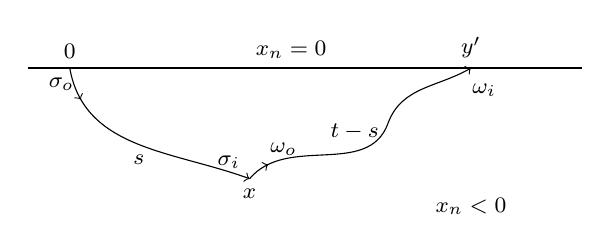
\begin{tikzpicture}[middlearrow/.style ={
        decoration={             
            markings, 
            mark=at position 0.15 with {\arrow{>}}
        },
        postaction={decorate}
    },]
	\draw (-100pt,0) -- (100pt,0);
	\node[above] at (-5pt,0) {\footnotesize$x_n=0$};
	\node[above] at (60pt,0) {\footnotesize$y'$};
	\node at (60pt,-50pt) {\footnotesize $x_n < 0$};
	%\node at (-85pt,0) {\footnotesize$\times$};
%	\node at (-20pt,40pt) {\footnotesize$\times$};
	\node[below] at (-20pt,-40pt) {\footnotesize$x$};
	\node[above] at (-85pt,0) {\footnotesize $0$};
	\node[below left] at (-80pt,0) {\footnotesize $\sigma_o$};
	%\draw[->] (-85pt,0pt) to [out=280,in=240] (-80pt,-8pt); 
	\draw[->,middlearrow] (-85pt,0pt) to [out=280,in=160] (-20pt,-40pt);
	%\node at (-85pt,0pt) (starta) {};
	%\node at (-20pt,-40pt) (stopa) {};
	%\draw[red] (starta) to [out=280,in=160] ($(starta)!0.3!(stopa)$);
	%\draw (-40pt,-20pt) to [out=45,in=190] (-20pt,-40pt);
	\draw[middlearrow] (-20pt,-40pt) to [out=50,in=250] (30pt,-20pt);
	%\node at (-20pt,-40pt) (start) {};
	%\node at (30pt,-20pt) (stop) {};
	%\draw[red,<-] (start) to [out=280,in=160] ($(start)!0.3!(stop)$);
	%\draw[->] (-30pt,-37pt) to [out=17,in=190] (-20pt,-40pt);
	\node[above left] at (-20pt,-40pt) {\footnotesize $\sigma_i$};
	%\draw[->] (-20pt,-40pt) to [out=320,in=130] (-15pt,-35.5pt);
	\node[above right] at (-16pt,-35pt) {\footnotesize $\omega_o$};
	\draw[->] (30pt,-20pt) to [out=70,in=210] (60pt,0pt);
	%\draw[->] (63pt,-10pt) to [out=254,in=210] (60pt,0pt);
	\node[right] at (57pt,-8pt) {\footnotesize $\omega_i$};
	\node at (-60pt,-33pt) {\footnotesize $s$};
	\node at (18pt,-23pt) {\footnotesize $t-s$};
	\end{tikzpicture}
	\caption{The points $0, x$ and $y'$ marked in space. The arrows indicate the (outgoing and incoming) momenta $\sigma_o = \exp_0^{-1}(x)$ and $\sigma_i = -\exp_x^{-1}(0)$ for the first part of the broken ray. The arrows marked $\omega_0$ and $\omega_i$ are the analogous momenta for the second part of the ray. The symbol $s$ indicates the time $s=d_c(x,0)$ to travel from $0$ to $x$. Note that if $(x,\xi) \in \pi_R \Lambda$, then (after unit normalization of $\sigma_i,\omega_o$) we have $\xi = \sigma_i-\omega_o$, the `reflection' angle, in some sense. Furthermore, if $(t,y',\tau,\zeta') \in \pi_L\Lambda$, then $\zeta'=-\omega_i'$ (or a scalar multiple thereof).}
	%The arrows indicate the momenta at these points $\sigma$ for outgoing momentum at $0$, $\phi_x, \theta$ for incoming and outgoing momenta at $x$ respectively, and $\phi_z$ for incoming momentum at $(y',0)$. The symbols $s'$ and $t-s'$ indicate the time traveled along the ray from $0$ to $x$ and from $x$ to $(y',0)$ respectively.}
	\label{fig:raypic}
\end{figure}


	First we note that since $t>0$, on the support of $c_\delta$ ($x$ away from the surface $\{y_n=0\}$), the set $\Lambda$ is a well-defined analytic canonical relation corresponding to the phase $\theta(t-d_c(y',x)-d_c(x,0))$.

	We now proceed to check that $\Lambda$ and the phase $\theta(t-d_c(y',x)-d_c(x,0))$ are salutary according to \cref{def:admisCR,def:bolkone} and that \cref{eq:extraWFempty} holds for $\Lambda$.  Let $(t,y',x,\theta)\in \Sigma$.

	\begin{enumerate}[leftmargin=*,listparindent=\parindent]
		\item To check \cref{eq:extraWFempty} we must verify that $\frac{\exp_x^{-1}(y')}{d_c(y',x)}+\frac{\exp_x^{-1}(0)}{d_c(x,0)} \neq 0$. Note that for two vectors $u,v$ with $\abs{v}=\abs{u}=1$ we have
	\[
		u+v = 0 \iff \langle u+v,u+v\rangle = 0 \iff 2\langle u,v\rangle = -2 \iff \langle u,v\rangle = -1 \iff \arccos(\langle u,v\rangle) = \pi\,.
	\]
	Therefore, the failure of \cref{eq:extraWFempty} is equivalent to the statement that the reflection angle
	\[
		\arccos\left(\left\langle \frac{\exp_x^{-1}(y')}{d_c(y',x)}, \frac{\exp_x^{-1}(0)}{d_c(x,0)} \right\rangle\right) = \pi\,,
	\]
	which is precluded by \cref{eq:piscatter} (because from $(t,y',x,\theta)\in \Sigma$ we know that $x_n <0$).

	\item We see immediately that \ref{as:n4} is satisfied since the time-derivative of the phase is $\theta$, the frequency.

	\item The truth of \ref{as:n3} is implied by the fact that $\left(\theta,\theta\frac{(\exp_{y'}^{-1}(x))'}{d_c(y',x)}\right) \neq 0$ for $\theta\neq 0$.

	\item Checking \ref{as:n2} reduces to showing that $\frac{\exp_x^{-1}(y')}{d_c(y',x)}+\frac{\exp_x^{-1}(0)}{d_c(x,0)} \neq 0$, which, exactly as in checking \cref{eq:extraWFempty}, is precluded by \cref{eq:piscatter}.
	\end{enumerate}

	Thus, the proof of \cref{thm:waveFIO} is complete once we prove
	\begin{lemma}\label{lem:bolker}
		The canonical relation $\Lambda$ defined in \cref{eq:CR} satisfies the Bolker condition, \ref{as:n1}.
	\end{lemma}
	\end{proof}
\begin{proof}[Proof of \cref{lem:bolker}]
	We begin with the injectivity of $\pi_L$. 

	Let
	\[
		\left(d_c(y',x_0)+d_c(x_0,0),y',\theta,\theta \frac{(\exp_{y'}^{-1}(x_0))'}{d_c(y',x_0)};x_0,-\theta \left(\frac{\exp_{x_0}^{-1}(y')}{d_c(y',x_0)}+\frac{\exp_{x_0}^{-1}(0)}{d_c(x_0,0)}\right)\right) \in \Lambda
	\]
	and
	\[
		 \left(d_c(y',x_1)+d_c(x_1,0),y',\theta,\theta \frac{(\exp_{y'}^{-1}(x_1))'}{d_c(y',x_1)};x_1,-\theta \left(\frac{\exp_{x_1}^{-1}(y')}{d_c(y',x_1)}+\frac{\exp_{x_1}^{-1}(0)}{d_c(x_1,0)}\right)\right) \in \Lambda
	\]
	satisfy
	\[
		(t,\zeta') \coloneqq \left(d_c(y',x_0)+d_c(x_0,0),\frac{(\exp_{y'}^{-1}(x_0))'}{d_c(y',x_0)}\right) = \left(d_c(y',x_1)+d_c(x_1,0),\frac{(\exp_{y'}^{-1}(x_1))'}{d_c(y',x_1)}\right)\,.
	\]
	We want to show that $x_0 = x_1$. 

	Note that for $j\in\{0,1\}$,
	\[
		1= \abs{\frac{\exp_{y'}^{-1}(x_j)}{d_c(y',x_j)}}^2\,,\quad \text{so that}\quad (\exp_{y'}^{-1}(x_j))_n = \sqrt{1 - \abs{\frac{(\exp_{y'}^{-1}(x_j))'}{d_c(y',x_j)}}^2} = \sqrt{1-\abs{\zeta'}^2}
	\]
	where the RHS of the second equation is analytic in $\zeta'$ due to \cref{eq:nograze}. We took the positive square root which corresponds to the ray coming from below the surface.

	We thus define $\zeta \coloneqq \left(\zeta', \sqrt{1-\abs{\zeta'}^2}\right)$, which has norm $1$ and have
	\[
		x_j = \exp_{y'}\left(d_c(x_j,y') \zeta\right)\,,\quad j\in\{0,1\}\,,%\quad\left(\text{or equivalently}\quad \zeta = \frac{\exp_{y'}^{-1}(x_j)}{d_c(x_j,y')}\right)
	\]
	so that showing that $d_c(x_0,y')=d_c(x_1,y')$ will imply that $x_0 = x_1$, which will prove the injectivity of $\pi_L$.

	We now define two functions
	\[
		x(s) = \exp_{y'}(s\zeta)\,,\an f(s) = t-s-d_c(x(s),0)
	\]
	and note that $x_j = x(d_c(x_j,y'))$ and $f(d_c(x_j,y')) = 0$ for $j\in\{0,1\}$. 

	Notice first that $x(s)$ is a smooth function for $s>0$ and that it satisfies
	\[
		\nabla x(s) = \del_h \exp_{y'}((s+h)\zeta)\vert_{h=0} = D\exp_{y'}(s\zeta)\zeta\,,	
	\]
	and by the Gauss lemma \cite[Thm.~6.2]{ilmavirta2020geometry} and the fact that $\abs{\zeta}=1$ we have
	\[
		\abs{\nabla x(s)}^2 = \langle \nabla x(s),\nabla x(s)\rangle = \frac{1}{s}\langle D\exp_{y'}(s\zeta)s \zeta,D\exp_{y'}(s\zeta)\zeta\rangle = \frac{1}{s} \langle s\zeta, \zeta\rangle = 1\,.
	\]
	Note further that because $\abs{\zeta}=1$ we have $d_c(x(s),y')=s$ and thus 
	\[
		0 = \del_s(s-d_c(x(s),y')) = 1+\frac{\exp_{x(s)}^{-1}(y')}{d_c(x(s),y')}\nabla x(s)\,,
	\]
	and because $\nabla x(s)$ and $\frac{\exp_{x(s)}^{-1}(y')}{d_c(x(s),y')}$ both have norm $1$, we must have that
	\begin{equation}\label{eq:nablax}
		\nabla x(s) = - \frac{\exp_{x(s)}^{-1}(y')}{d_c(x(s),y')}\,.
	\end{equation}
	We remark that \cref{eq:nablax} is also seen intuitively if one were to draw a picture of the ray $x(s)$. 

	Notice also that $f$ is a smooth function for $s>0$ and its derivative is 
	\[
		f'(s) = -1+\frac{\exp_{x(s)}^{-1}(0)}{d_c(x(s),0)}\cdot \nabla x(s)\,,
	\]
	where both vectors $\frac{\exp_{x(s)}^{-1}(0)}{d_c(x(s),0)}$ and $\nabla x(s)$ have norm $1$, so that
	\[
		f'(s) =0 \iff \left\langle \frac{\exp_{x(s)}^{-1}(0)}{d_c(x(s),0)}, \nabla x(s)\right\rangle = 1\,.
	\]
	Therefore, using \cref{eq:nablax},%that $\nabla x(s) = -\frac{\exp_{x(s)}^{-1}(y')}{d_c(x(s),y')}$,

	\[
		f'(s) =0 \iff \left\langle \frac{\exp_{x(s)}^{-1}(0)}{d_c(x(s),0)}, \frac{\exp_{x(s)}^{-1}(y')}{d_c(x(s),y')}\right\rangle = -1\,,
	\]
	which again is precluded by \cref{eq:piscatter}.

	We therefore see that $f$ is a smooth function with non-vanishing derivative for $s>0$. Therefore, it attains at most one zero in $s>0$, and since both $d_c(x_0,y')$ and $d_c(x_1,y')$ are zeroes of $f$ and neither of these distances is $0$ by \cref{eq:piscatter}, we must have $d_c(x_0,y')=d_c(x_1,y')$.
	
	We have thus concluded that $x_0 = x_1$, wherefore $\pi_L$ is injective. 

%
%
%
%
%	We first show that we can recover the momentum from $y'$ generates a ray hitting $x$ after positive time. We use the fact that we know that for all $x$ and all $y$ away from $x$, the function $\phi(t,y,\theta) = (t-d_c(y',x))\theta$ satisfies the Eikonal equation of the wave equation: $\abs{\phi_t}^2 - c_0^2(y)\abs{\phi_y}^2 = 0$. Then we use the fact that $\phi_\theta =0$ means there is a ray from $y'$ taking $t$ time to travel to $x$ (see \cite[Exc.~2.1]{MR597145} or \cite{MR0516965}), and furthermore, $\del_y \phi$ is the momentum of this ray. 
%
%	Since $\varphi_y = \theta d_c(y,x)^{-1}\exp^{-1}_y(x)$, we have in particular that
%	\[
%		(\exp^{-1}_y(x))_n = \sqrt{1-\frac{c_0^2(y)}{d_c^2(y,x)}\abs{(\exp_{y}^{-1}(x))'}^2}
%	\]
%	where $(\exp_{y}^{-1}(x))'$ are the first $n-1$ components, and we took the positive square root corresponding to a ray coming from below. The map on the RHS is $0$ if the vertical component vanishes, in which case the map is no longer analytic there. However, due to the assumption of no grazing rays this map is analytic since the RHS never vanishes.
%
%	Now $\del_{y'}d_c(y',x) = (\del_y d_c(y',x))'$ so that the information 
%	\[
%		(z,\zeta) = (t,y',\theta,\theta\del_{y'}d_c(y',x))
%	\]
%	allows us to fully recover $\del_{y}d_c(y',x)$, the full initial momentum from $y'$ to $x$. Therefore, we have determined a ray from $y'$ that will hit both $x_0$ and $x_1$. We know there are rays from both $x_0$ and $x_1$ to the origin and the total travel time along both is the same. The assumption of no conjugate points precludes the option that $x_0\neq x_1$, so that indeed we have shown that $\pi_L$ is injective. 
	Thus, let us turn to showing that $\pi_L \colon \Lambda \to T^\ast((0,T)\times\mathcal{M}')\sem$ is an immersion. This will follow from the fact that $\pi_R \colon \Lambda \to T^\ast\mathcal{M}\sem$ is a submersion and \cite[Lem.~4.3]{zbMATH01860565}.%, and the fact that $\dim T^\ast((0,T)\times \mathcal{M}') = \dim T^\ast(\mathcal{M}) = 2n$.

	We will show that for any $(x_0,\xi_0) \in \pi_R(\Lambda)$, for some analytic function $\alpha$,
	\[
		 \left\{(\alpha(x,\xi); x,\xi) \colon (x,\xi)\ \text{near}\ (x_0,\xi_0)\right\} = \Lambda \cap \{\text{an open neighborhood of}\ \pi_R^{-1}((x_0,\xi_0))\}\,,%\left\{\pi_R^{-1}((x,\xi))\colon \pi_R(\Lambda) \ni (x,\xi)\ \text{near} \ (x_0,\xi_0)\right\}
	\]
	from which one can readily see that $\pi_R$ must be a submersion.

	%First, let $x \in \RR^n$ with $x_n < 0$. Then there is a ray from $0$ to $x$, and because we assumed no conjugate points, there is precisely one bicharacteristic from $0$ to $x$ and this bicharacteristic has non-zero momentum $-\exp_{x}^{-1}(0)$ at $x$, and length $s = d_c(x,0)$.

	Throughout the rest of this proof, for any vector $u$, the notation $u'$ refers to the first $n-1$ components of $u$. Let $(x,\xi)$ near $(x_0,\xi_0) \in \pi_R(\Lambda)$.

	By \cref{eq:CR},
	\[
		(t,y',\theta,\zeta';x,\xi) \in \Lambda \iff F(t,y',\theta,\zeta';x,\xi)\coloneqq \begin{pmatrix}t-d_c(x,0)-d_c(x,y')\\\begin{pmatrix}y' \\ 0\end{pmatrix}-\exp_x\left((t-d_c(x,0))\left(-\frac{\xi}{\theta}-\frac{\exp_x^{-1}(0)}{d_c(x,0)}\right)\right)\\ \zeta' -\theta\frac{(\exp_{y'}^{-1}(x))'}{d_c(x,y')}\end{pmatrix} = 0\,.
	\]
	%then 
	%\[
	%	y' = \left[\exp_x\left((t-d_c(x,0))\left(\frac{\xi}{\abs{\xi}}+\frac{\exp_x^{-1}(0)}{d_c(x,0)}\right)\right)\right]'
	%\]
	%where by $[\dots]'$ we mean the first $n-1$ components of the given vector. 
	We will want to appeal to the implicit function theorem to show that $F = 0 \iff (t,y',\theta,\zeta') = \alpha(x,\xi)$ for some analytic function $\alpha$. 

	Because $(x_0,\xi_0)\in \pi_R(\Lambda)$, there is some $(t_0,y'_0,\theta_0,\zeta_0')$ so that $F(t_0,y_0',\theta_0,\zeta_0';x_0,\xi_0) = 0$. Throughout the rest of this proof, to lighten notation we write $(t,y',\theta,\zeta';x,\xi)$ for $(t_0,y_0',\theta_0,\zeta_0';x_0,\xi_0)$, the argument of $F$ will always be this point.

	%Thus, for some point where $F=0$, we check the derivative. 
	Let us introduce the shorthands
	\[
		v \coloneqq \left(-\frac{\xi}{\theta}-\frac{\exp_x^{-1}(0)}{d_c(x,0)}\right)\,,\quad  G \coloneqq (D\exp_x)\left((t-d_c(x,0))\left(-\frac{\xi}{\theta}-\frac{\exp_x^{-1}(0)}{d_c(x,0)}\right)\right) = (D\exp_x)\left((t-d_c(x,0))v\right)
	\]
	and note that $\abs{v} = 1$ because $F=0$, because then $v = \frac{\exp_x^{-1}(y')}{d_c(x,y')}$ by \cref{eq:CR}.

	We calculate (where $\ast$ refers to some expression we do not explicitly calculate):
	\[
		\del_{(t,y',\theta,\zeta')}F = \begin{pmatrix} 1 & \frac{(\exp_{y'}^{-1}(x))'}{d_c(x,y')} & 0 & 0 \\
		-(Gv)' & \id' & (\theta^{-1}(t-d_c(x,0))G(-\frac{\xi}{\theta}))' & 0 \\
		-(Gv)_n & 0 & (\theta^{-1}(t-d_c(x,0))G(-\frac{\xi}{\theta}))_n & 0 \\
		0 & \ast & \ast & \id'\end{pmatrix}
	\]
	which is invertible if and only if the matrix
	\[
		K \coloneqq \begin{pmatrix} 1 & \frac{(\exp_{y'}^{-1}(x))'}{d_c(x,y')} & 0  \\
		-(Gv)' & \id' & (\theta^{-1}(t-d_c(x,0))G(-\frac{\xi}{\theta}))'  \\
		-(Gv)_n & 0 & (\theta^{-1}(t-d_c(x,0))G(-\frac{\xi}{\theta}))_n\end{pmatrix}
	\]
	is invertible.

	%From hereon out we take $F=0$ so that $\abs{v}=1$ and $t-d_c(x,0)=d_c(x,y')$. 

	Putting $y(s) \coloneqq \exp_x(s v)$, we proceed as in the proof of the injectivity of $\pi_L$ to calculate that because $d_c(y(s),x) = s$, we have by differentiation with respect to $s$ that
	\[
		-1 = \frac{\exp_{y(s)}^{-1}(x)}{d_c(y(s),x)}\cdot \dot y(s)\,,
	\]
	where by the Gauss lemma and the fact that $\abs{v}=1$ we find that $\abs{\dot y(s)}=1$, so that we may conclude that 
	\[
		\dot y(s) = -\frac{\exp_{y(s)}^{-1}(x)}{d_c(y(s),x)}\,,
	\]
	and since $y' = y(d_c(x,y')) = y(t-d_c(x,0))$ (here $y$ is the function $y(s)$), we find
	\[
		\frac{\exp_{y'}^{-1}(x)}{d_c(x,y')} = -\del_s \exp_x((t-d_c(x,0)+s)v)\vert_{s=0} = -Gv\,,
	\]
	which we can insert into the matrix $K$.

	Using elementary matrix operations to remove the entries to the left and right of the central $\id'$, we see that $K$ is invertible if and only if 
	\[
		\begin{pmatrix} 1- \langle (Gv)',(Gv)'\rangle & -(Gv)' & \theta^{-1}(t-d_c(x,0))\langle (G(-\frac{\xi}{\theta}))',(Gv)'\rangle  \\
		0 & \id' & 0  \\
		-(Gv)_n & 0 & (\theta^{-1}(t-d_c(x,0))G(-\frac{\xi}{\theta}))_n\end{pmatrix}
	\]
	is invertible.

	This is true if and only if the $2$-vectors
	\[
		\begin{pmatrix} 1- \langle (Gv)',(Gv)'\rangle  \\ -(Gv)_n \end{pmatrix},\an\begin{pmatrix} \theta^{-1}(t-d_c(x,0))\langle (G(-\frac{\xi}{\theta}))',(Gv)'\rangle \\ (\theta^{-1}(t-d_c(x,0))G(-\frac{\xi}{\theta}))_n\end{pmatrix}
	\]
	are linearly independent and non-zero. 

	Now define $w \coloneqq \frac{\exp_x^{-1}(0)}{d_c(x,0)}$, which has norm $1$, and note that
	\begin{equation}\label{eq:vplusw}
		\frac{-\xi}{\theta} = v+w\,.
	\end{equation}
	
	Use Gauss' lemma \cite[Thm.~6.2]{ilmavirta2020geometry} %(or see \cite[Thm.~6.9]{zbMATH06897812}) 
	again to write that
	\[
		\langle (Gv)',(Gv)'\rangle = \langle Gv,Gv\rangle - (Gv)_n^2 = \langle v,v\rangle -(Gv)_n^2 = 1- (Gv)_n^2\,,
	\]
	and using \cref{eq:vplusw},
	\[
		\left\langle \left(G\left(-\frac{\xi}{\theta}\right)\right)',(Gv)'\right\rangle = \langle Gv,Gv\rangle - (Gv)_n^2 + \langle Gw,Gv\rangle - (Gw)_n(Gv)_n = 1 - (Gv)_n^2 + \langle w,v\rangle - (Gw)_n(Gv)_n\,.
	\]
	So that we must check that 
	\[
		\begin{pmatrix} (Gv)_n^2  \\ -(Gv)_n \end{pmatrix},\an\begin{pmatrix} 1 + \langle w,v\rangle - (Gv)_n^2 - (Gw)_n(Gv)_n\\ (Gw)_n + (Gv)_n\end{pmatrix}
	\]
	are non-zero and linearly independent. 

	The first of these vectors is non-zero by assumption of no grazing rays \cref{eq:nograze}: $(Gv)_n = -\left(\frac{\exp_{y'}^{-1}(x)}{d_c(x,y')}\right)_n \neq 0$ (again since we must have $x_n < 0$), whereas the second vector vanishes if and only if $1+\langle w,v\rangle =0$, which is (due to the fact that $\abs{v}=\abs{w}=1$) equivalent to $w = -v$, which is precluded exactly by the assumption of no scattering over $\pi$, \cref{eq:piscatter}.

	Finally, checking that the vectors are linearly independent reduces to showing that $1 + \langle w,v\rangle \neq 0$, which is still true by \cref{eq:piscatter}.

	We have thus shown that $\del_{(t,y',\theta,\zeta')}F$ is invertible at the point $(t,y',\theta,\zeta';x,\xi)=(t_0,y_0',\theta_0,\zeta_0';x_0,\xi_0)$, so that an application of the implicit function theorem completes the proof.
\end{proof}

%%%%As a consequence of \cref{lem:roughsc} and the proof of the above theorem, we state without proof
%%%%\begin{lemma}\label{lem:roughda}
%%%%	Let $k_0 \in \mathbb{N}$, there exist $k,N\in\mathbb{N}$ so that if $c \in C^k, c>0$ 
%%%%	%When $c \in C^k, c>0$ 
%%%%	gives rise to a simple metric
%%%%	\[
%%%%		DA[c](c_\delta) = \int e^{i\theta(t-d_c(y',x)-d_c(x,0))}b(y',x,\theta)\dd\theta c_\delta(x)\dd x\mod C^{k_0}((0,T)\times \mathcal{M}')
%%%%	\]
%%%%	with $b\in C^{k_0}S^{n-1}$. The seminorms of $b$ depend on $c$ as follows:
%%%%	\[
%%%%		\sup_{\abs{\alpha},\abs{\beta},\abs{\gamma} \leq k_0} \abs{\del^\alpha_x\del^\beta_{y'} \del^\gamma_\theta b(y',x,\theta)} \leq C\norm{c}_{C^{k_0+m}}
%%%%	\]
%%%%	for some $m$ bla that will come from the prev lemma.
%%%%\end{lemma}
%%%%
%%%%	

%
%
%
%\begin{theorem}\label{thm:waveFIO}
%	Let the background geometry $c_0$ contain no grazing rays: bicharacteristic rays starting in $x_n < -\eps$ do not arrive at $x_n = 0$ with momentum whose $n$-th component is $0$.
%
%	There are two lacunary triplets $(b^+,\varphi,\Gamma), (b^-,\varphi,\Gamma)$  with associated lacunary FIO $T^+, T^-$ respectively, so that the following holds. \marginnote{refer to def of lac triplets}
%
%	Restricted to $\Gamma$, the amplitudes $b^\pm$ are finite realizations of an elliptic formal amplitude $\ud{b}^\pm\in FS^{-1}_{\psi a}(\Gamma)$ and modulo analytically regularizing terms,
%	\[
%		C^\infty_c(\RR^{n}_\eps) \ni p \mapsto DA[c_0](p) = \del_t^2 T^{+}(p) + \del_t^2 T^{-}(p)\,.
%	\]
%	%with salutary analytic phases $\varphi^\pm$ and the canonical relation $\Lambda^\pm$ of the FIO $DA[c_0]^\pm$ satisfies \cref{eq:extraWFempty}.
%\end{theorem}
%
%\begin{proof}[Proof of \cref{thm:waveFIO}]
%	
%
%	Let $\phi^\pm$ and $\ud{a}^\pm \in \mathrm{FS}^0_1$ be the non-degenerate analytic phase and formal elliptic amplitude from \cref{cor:solvewave}, and let $a^\pm \in S^0_1$ be a finite realization of $\ud{a}^\pm$.
%
%	According to the description \cref{eq:firstDA} and \cref{cor:solvewave} we get that 
%	\[
%	DA[c_0](p) = DA[c_0]^{+,+}(p) + DA[c_0]^{+,-}(p) + DA[c_0]^{-,+}(p) + DA[c_0]^{-,-}(p)\,,
%	\]
%	where $DA[c_0]^{\pm_1,\pm_2} = \del_t^2 \circ T^{\pm_1,\pm_2}$ and $T^{\pm_1,\pm_2}\colon C_c^\infty(\RR^n_\eps) \ni p \mapsto \DD'(\RR^n)$ is the operator
%	\begin{equation}\label{eq:defTpm}
%		T^{\pm_1,\pm_2}(p) = 
%		\int_{-\infty}^t\hspace{-0.5mm}\iiint e^{i(\phi^{\pm_1}(t-s,y',\theta)-x\cdot \theta+ \phi^{\pm_2}(s,x,\sigma))} \td{b}^{\pm_1,\pm_2}(t,y',x,\theta,\sigma,s) \dd \sigma\dd\theta p(x) \dd x \dd s
%	\end{equation}
%	where
%	\[
%		\td{b}^{\pm_1,\pm_2}(t,y',x,\theta,\sigma,s) = a^{\pm_1}(t-s,y',\theta)c_0^2(x)a^{\pm_2}(s,x,\sigma)c_0^2(0)\,.
%	\]
%
%	\bsc{1. Remove cut-off in time $s$}
%
%	Notice that at $s=t$ we have $\phi^{\pm_1}_\theta(t-s,y',\theta)=y'=(y',0)$ due to \cref{eq:phipos}, so we may conclude that $\phi^{\pm_1}_\theta(t-s,y',\theta)_n  > -\eps$ for $s$ near $t$. Furthermore, on the stationary set of $\phi^{\pm_1}$ we have $\phi^{\pm_1}_\theta(t-s,y',\theta)=x$, so that we may conclude
%	\[
%		s\ \text{near}\ t\ \text{and}\ (t-s,y',\theta)\ \text{near}\ \{\phi_\theta^{\pm_1}(t-s,y',\theta) = x\}\implies x_n > -\eps\,.
%	\]
%	In addition, after invoking \cref{rem:acutoff}, we may assume that for any small $\delta>0$ and $s>t+\delta$ we have $a^\pm_1(t-s,y',\theta) =0$, so that $\td{b}^{\pm_1,\pm_2}(t,y',x,\theta,\sigma,s) = 0$ for $s>t+\delta$.
%
%	Therefore, for $s \geq t$ we may conclude that
%	\[
%		(t,y',x,\theta,\sigma,s) \in \{\phi^{\pm_1}_\theta(t-s,y',\theta)=x\,, \phi^{\pm_2}_\sigma(s,x,\sigma)=0\} \cap \supp \td{b} \implies x_n > -\eps \implies x \not\in \supp p
%	\]
%	since $\supp p \subset \RR^n_{\eps}$. 
%
%	We may thus conclude from \cref{prop:wfaexp} that for $s \geq t$, the operator
%	\[
%		p \mapsto \iiint e^{i(\phi^{\pm_1}(t-s,y',\theta)-x\cdot \theta+ \phi^{\pm_2}(s,x,\sigma))} \td{b}^{\pm_1,\pm_2}(t,y',x,\theta,\sigma,s) \dd \sigma\dd\theta p(x) \dd x
%	\]
%	has empty $\wf$. 
%
%	Therefore, since the integrand in \cref{eq:defTpm} is analytic with respect to $s$, up to analytically regularizing operators, 
%	\[
%	T^{\pm_1,\pm_2}(p) = 
%		\iiiint e^{i(\phi^{\pm_1}(t-s,y',\theta)-x\cdot \theta+ \phi^{\pm_2}(s,x,\sigma))} \td{b}^{\pm_1,\pm_2}(t,y',x,\theta,\sigma,s) \dd \sigma\dd\theta\dd s
%p(x) \dd x 	
%	\]
%	where we swapped the order of integration between $x$ and $s$ because the integrand is compactly supported with respect to these two variables. 
%
%	\bsc{2. Make $s$ frequency variable}
%
%	Using the fact that for $\abs{\sigma},\abs{\theta}$ small enough, $a^\pm = 0$ and thus $\td{b} = 0$, we may use substitution $s \mapsto (\abs{\sigma}+\abs{\theta})s$ and define new variables $z=(t,y')$ and $\eta=(\theta,\sigma,s)$ so that for $T^{\pm_1,\pm_2}$ from \cref{eq:defTpm}, modulo analyticically regularizing terms,
%	\[
%	T^{\pm_1,\pm_2}(p) = \iint e^{i\varphi^{\pm_1,\pm_2}(z,x,\eta)}b_1^{\pm_1,\pm_2}(z,x,\eta) \dd\eta p(x) \dd x
%	\]
%	where
%	\[
%		b_1^{\pm_1,\pm_2}(z,x,\eta) = \td{b}^{\pm_1,\pm_2}\left(t,y',x,\theta,\sigma,\frac{s}{\abs{\theta}+\abs{\sigma}}\right)({\abs{\theta}+\abs{\sigma}})^{-1}
%	\]
%	and
%	\[
%		\varphi^{\pm_1,\pm_2}(z,x,\eta) = \phi^{\pm_1}\left(t-\frac{s}{\abs{\theta}+\abs{\sigma}},y',\theta\right)-x\cdot \theta+ \phi^{\pm_2}\left(\frac{s}{\abs{\theta}+\abs{\sigma}},x,\sigma\right)\,.
%	\]
%
%	Notice that the stationary set of $\varphi^{\pm_1,\pm_2}$ is 
%	\begin{align*}
%	\Sigma_\varphi^{\pm_1,\pm_2} %&= \left\{(z,x,\eta)\colon \phi^{\pm_1}_\sigma(t',x,\sigma)-\sigma\abs{\sigma}^{-1}\omega (s-t')=0, \phi^{\pm_2}_\theta(t-s,y,\theta)=x,s=t', \omega=\phi^{\pm_2}_t(t-s,y,\theta)=\phi^{\pm_1}_t(t',x,\sigma)\right\} \\
%		&= \left\{(z,x,\eta)\colon \phi^{\pm_2}_\sigma\left(\frac{s}{\abs{\theta}+\abs{\sigma}},x,\sigma\right)=0, \phi^{\pm_1}_\theta\left(t-\frac{s}{\abs{\theta}+\abs{\sigma}},y',\theta\right)=x,\right. \\
%		&\qquad\qquad\left.\phi^{\pm_1}_t\left(t-\frac{s}{\abs{\theta}+\abs{\sigma}},y',\theta\right)=\phi^{\pm_2}_t\left(\frac{s}{\abs{\theta}+\abs{\sigma}},x,\sigma\right)\right\}\,,
%	\end{align*}
%	which is the empty set if $\pm_1 \neq \pm_2$ due to the fact that from \cref{eq:phipos} we can conclude
%	\[
%		\mp_2\phi^{\pm_2}_t(s,x,\sigma) < 0 < \pm_1\phi^{\pm_1}_t(t-s,y',\theta)\,.
%	\]
%	Thus, from \cref{prop:wfaexp} we see that
%	\[
%		\wf(p \mapsto T^{+,-}(p)) = \emptyset = \wf(p \mapsto T^{-,+}(p))\,,
%	\]
%	and in particular $DA[c_0]^{+,-}$ and $DA[c_0]^{-,+}$ are analytically regularizing. 
%
%	\bsc{3. Non-Degenerate Phase}
%
%	From this point onward we drop the notation $\pm$ in $\varphi^{\pm} = \varphi^{\pm,\pm}$ and $T^{\pm} = T^{\pm,\pm}$.
%
%	We know that $\varphi(z,x,\eta)$ is an analytic function that is homogeneous of degree $1$ with respect to $\eta$. Furthermore, since $\phi_\theta(t-s,y',\theta) = 0 \implies \phi_t(t-s,y',\theta) \neq 0$ (see \cref{eq:phipos}), we know that 
%	\[
%		\nabla_{(z,\eta)} \varphi \neq 0\,.
%	\]
%	Thus, in order to conclude that $\varphi$ is a non-degenerate analytic phase, the last property we need to deduce is the non-degeneracy of $\varphi$. The only difference between our phase here and the one in the proof of \cite[Lem.~2.2]{zbMATH04097945} is that we have already introduced the trace to $y_n =0$. However, the proof follows nearly identically so that we keep it very brief here. 
%
%	We will show that 
%	\[
%		\hat\varphi(z,x,\eta) = \phi\left(t-s,y',\theta\right)-x\cdot \theta+ \phi\left(s,x,\sigma\right)\,.
%	\]
%	is non-degenerate from which it will follow that $\varphi$ is non-degenerate. 
%	Following \cite[Lem.~2.2]{zbMATH04097945}, we introduce
%	\[
%		\Sigma_1 = \{(t,y', \phi_t, \phi_{y'};x,s,-\phi_x,-\phi_s)\colon \phi_\theta-x = 0\}\,,\an \Sigma_2 = \{(s,x, \phi_s, \phi_{x})\colon \phi_\sigma = 0\}
%	\]
%	and
%	\[
%		W = T^\ast(\RR^n) \times \mathrm{diag}(T^\ast \RR \times T^\ast \RR)\times \{(x,\xi^1;x,\xi^2)\colon x,\xi^1,\xi^2\in \RR^n\}
%	\]
%	where $\Sigma_1$ has dimension $2n+1$ and $\Sigma_2$ has dimension $n+1$ and $W$ has dimension $5n+2$.
%
%	Now $\varphi$ being non-degenerate is implied by the fact $\Sigma_1\times\Sigma_2$ is transverse to $W$ in $T^\ast(\RR^n\times \RR^{n+1})\times T^\ast(\RR^{n+1})$, which is reduced to showing that the map
%	\[
%		\Sigma_1\times\Sigma_2 \mapsto \RR^{n+2}\,, (t,y',\tau,\zeta';x^1,s^1,\xi^1,\sigma^1)\times (x^2,s^2,\xi^2,\sigma^2) \mapsto (x^1-x^2,s^1-s^2,\sigma^1-\sigma^2)
%	\]
%	has rank $n+2$ in $\Sigma_1\times\Sigma_2 \cap W$. 
%
%	Now notice that $\phi_\theta(t_0-s_0,y_0',\theta_0) = x_0$ (with initial condition $\phi_\theta(0,y_0',\theta_0) = y_0'$) corresponds to the situation that there is a ray starting at $x_0$ with initial momentum $\theta_0$ that takes $t_0-s_0$ time to travel to $y'_0$ and arrives with momentum $\phi_y(t_0-s_0,y'_0,\theta_0)$. Now due to the assumption of no grazing rays we know that $\phi_{y_n}(t_0-s_0,y'_0,\theta_0)$ is away from $0$, so that the ray is pointing upward toward the surface. Thus, perturbing $(s,x,\theta)$ around $(s_0,x_0,\theta_0)$, the ray starting at $x$ with momentum $\theta$ will lie close to $y_0'$ after $t_0-s$ time and be pointing upward there, so that in fact it will hit the surface $\{y_n = 0\}$, yielding some $y'$ and $t$ so that $\phi_\theta(t-s,y',\theta) = x$. 
%
%	Therefore, $\{\phi_\theta = x\}$ is locally parametrized by $(t,\theta,x)$, so that $\Sigma_1$ is locally parametrized by $(s^1,x^1,\xi^1)$. 
%
%	Now since the rays satisfy a Hamiltonian system, since $\xi^1\neq 0$, we know that
%	\[
%		c_0^2(x^1) (\sigma^1)^2 = \abs{\xi^1}^2\,,\an \del_{\xi^1} \sigma^1 = c_0^{-2}(x^1) (\sigma^1)^{-1} \xi^1 \neq 0\,.
%	\]
%	
%	This concludes the proof that $\hat\varphi$ is non-degenerate, yielding that $\varphi$ is non-degenerate.
%
%	\bsc{4. Lacunary Triplet}
%
%%	Notice that if $\nabla_x\varphi(z,x,\eta) =0$, then $\theta = \phi^\pm(\frac{s}{\abs{\theta}+\abs{\sigma}},x,\sigma)$, so that
%%	\[
%%		(z,x,\eta)\in \Sigma\ \text{and}\ \nabla_x\varphi^\pm(z,x,\eta) =0 \implies \text{scattering over}\ \pi\,,
%%	\]
%%	which we assumed did not happen. Therefore we can conclude that 
%%	\begin{equation}\label{eq:nosca}
%%		\nabla_x\td{\varphi}^\pm(t,y,s,x,\theta,\sigma) =0 \implies \abs{\eta}^{-1}\abs{\nabla_\eta\td{\varphi}^\pm(t,y,s,x,\theta,\sigma)} > 0\,,
%%	\end{equation}
%%	uniformly on $\abs{\theta}+\abs{\sigma}=1$.
%
%	Since the operator defined by its kernel will be $T \in \DD'(\RR^n\times \RR^n)$, we may assume that $z$ (in particular $t$) and $x$ range in a compact set. \marginnote{do I need this?}
%
%	This part of the proof is inspired by an argument in the proof of \cite[Thm.~25.2.3]{zbMATH05528184}. 
%
%	Notice that
%	\[
%		\nabla_x\varphi(z,x,\eta) = \theta + \nabla_x \phi\left(\frac{s}{\abs{\theta}+\abs{\sigma}},x,\sigma\right)\,,
%	\]
%	where due to \cref{eq:phipos}, we know $\nabla_x \phi_x\left(\frac{s}{\abs{\theta}+\abs{\sigma}},x,\sigma\right) \neq 0$ for $\sigma\neq 0$.
%	
%	Thus, there exist $c,C > 0$ so that
%	\[
%		\nabla_x \varphi(z,x,\eta) = 0 \implies c\abs{\theta} \leq \abs{\sigma} \leq C\abs{\theta}\,.
%	\]
%
%	Notice that if $(z,x,\eta) \in \Sigma$, the stationary set of $\varphi$, then on the support of $b_1$ (here $\sigma,\theta\neq 0$),
%	\begin{equation}
%		\phi_t\left(t-\frac{s}{\abs{\theta}+\abs{\sigma}},y',\theta\right) = \phi_t\left(\frac{s}{\abs{\theta}+\abs{\sigma}}, x,\sigma\right) \neq 0\,.
%	\end{equation}
%	Therefore, there are $c',C'>0$ so that 
%	\[
%		(z,x,\eta) \in \Sigma \implies c'\abs{\theta} \leq \abs{\sigma} \leq C'\abs{\theta}\,.
%	\]
%	
%	Now let $\Gamma$ be the conic set $\Gamma \coloneqq \{(\theta,\sigma,s)\colon \min\{c,c'\}/2\abs{\theta}\leq\abs{\sigma} \leq 2\max\{C,C'\}\abs{\theta}\}$ so that
%	\begin{equation}\label{eq:gammacomp}
%		(\theta,\sigma) \in \Gamma^c \implies \abs{\nabla_x\varphi(z,x,\eta)} > \td{C}(\abs{\theta} + \abs{\sigma})\,,
%	\end{equation}
%	for some $\td{C}>0$, and we have $\Sigma \subset \Gamma$. 
%
%	Since $s\leq t(\abs{\theta}+\abs{\sigma})$ on the support of $b$, we may thus conclude that 
%	\begin{equation}\label{eq:lac2}
%		\eta \in \Gamma^c \implies \abs{\nabla_x \varphi(z,x,\eta)} \geq C\abs{\eta}
%	\end{equation}
%	for some $C>0$.
%	
%	We will now show that $(b,\varphi,\Gamma)$ is a lacunary triplet as defined in \cref{def:lacunary}, where we have already shown one property in \cref{eq:lac2} and we have seen that $\Sigma\subset\Gamma$. Because $a \in S^0_{\psi a}(\RR^n)$ and $s\leq t(\abs{\theta}+\abs{\sigma})$ on the support of $b$, we find that $\abs{b}\leq C(1+\abs{\eta})^{-1}$ for some $C>0$.
%
%	Notice that on the support of $b$ we have that $s \leq C(\abs{\theta}+\abs{\sigma})$, so that
%	\[
%		\del_s^\alpha b(z,x,\eta) = (\del_s^\alpha \td{b})(z,x,\frac{s}{\abs{\theta}+\abs{\sigma}},\theta,\sigma) (\abs{\theta}+\abs{\sigma})^{-1-\abs{\alpha}}
%	\]
%	Since $\td{b} \in S^{0}_0$, and because $s\leq C(\abs{\theta}+\abs{\sigma})$, we see that 
%	\begin{equation}\label{eq:dels}
%		\abs{\del_s^\alpha b(z,x,\eta)} \leq (\abs{\theta}+\abs{\sigma})^{-1-\abs{\alpha}} \leq C^{\abs{\alpha}}\abs{\eta}^{-1-\abs{\alpha}}
%	\end{equation}
%	for some $C>0$.
%	
%	Due to the fact that $\abs{\varphi_s} > C$ on $\Gamma^\complement$, and because of \cref{eq:dels}, we see that in order to show that $(b,\varphi,\Gamma)$ is a lacunary triplet, we must only prove that for $\eta \in \Gamma$ we have $b \in S^{-1}_{\psi a}(\Gamma)$. 
%
%	Differentiating $b$ with respect to $s$ is covered in \cref{eq:dels}. Similarly, due to the fact that $a \in S^0_{\psi a}$, and the definition of $\Gamma$ from \cref{eq:gammacomp}, we see that differentiating $b$ with respect to $\theta$ or $\sigma$ reduces the order as we wish. We have therefore concluded that $b\in S_{\psi a}^{-1}(\Gamma)$, so that $(b,\varphi,\Gamma)$ is a lacunary triplet.
%
%	We will in fact also show that on $\Gamma$, the amplitude $b\in S^{-1}_{\psi a}(\Gamma)$ is the finite realization of a formal amplitude $\ud{b}\in \mathrm{FS}_{\psi a}^{-1}(\Gamma)$.
%
%	First, note that since each $a$ in the definition of $b$ is the finite realization of some $\ud{a}\in FS^0_{\psi a}$, we know that for some $R>0$ large enough,
%	\begin{align*}
%		b(z,x,\eta) &= (\abs{\theta}+\abs{\sigma})^{-1}c_0^2(x)c_0^2(0)\sum_{j\leq R^{-1}\abs{\theta}}a_j\left(t-\frac{s}{\abs{\theta}+\abs{\sigma}},y',\theta\right)\sum_{k\leq R^{-1}\abs{\sigma}}a_k\left(\frac{s}{\abs{\theta}+\abs{\sigma}},x,\sigma\right) \\
%		&=  (\abs{\theta}+\abs{\sigma})^{-1}c_0^2(x)c_0^2(0)\sum_{l \leq R^{-1}(\abs{\theta}+\abs{\sigma})}\sum_{\substack{j\leq R^{-1}\abs{\theta}\\k\leq R^{-1}\abs{\sigma}\\ j+k = l}}a_j\left(t-\frac{s}{\abs{\theta}+\abs{\sigma}},y',\theta\right)a_k\left(\frac{s}{\abs{\theta}+\abs{\sigma}},x,\sigma\right)
%	\end{align*}
%
%	Now define $\ud{b} = \sum_{l\geq 0} b_l$ where
%	\[
%		b_l(z,x,\eta) =  (\abs{\theta}+\abs{\sigma})^{-1}c_0^2(x)c_0^2(0)\sum_{j,k\in\mathbb{N},j+k = l}a_j\left(t-\frac{s}{\abs{\theta}+\abs{\sigma}},y',\theta\right)a_k\left(\frac{s}{\abs{\theta}+\abs{\sigma}},x,\sigma\right)\,.
%	\]
%	First, on the support of $b$ we have $s\leq t(\abs{\theta}+\abs{\sigma})$, and second, on $\Gamma$ we know that we can compare $\abs{\theta},\abs{\sigma}$, so that
%	\[
%		j+k=l\leq R^{-1} \abs{\eta} \implies j \leq \td{R}^{-1} \abs{\theta}\,, k\leq \td{R}^{-1}\abs{\sigma}\,,
%	\]
%	which means that finite realizations of $\ud{b}$ are given by 
%	\begin{align*}
%		&{}(\abs{\theta}+\abs{\sigma})^{-1}c_0^2(x)c_0^2(0)\sum_{l\leq R^{-1}\abs{\eta}}\sum_{j,k\in\mathbb{N},j+k = l}a_j\left(t-\frac{s}{\abs{\theta}+\abs{\sigma}},y',\theta\right)a_k\left(\frac{s}{\abs{\theta}+\abs{\sigma}},x,\sigma\right) \\
%		&\quad = (\abs{\theta}+\abs{\sigma})^{-1}c_0^2(x)c_0^2(0)\sum_{l\leq \td{R}^{-1}(\abs{\theta}+\abs{\sigma})}\sum_{\substack{j\leq R^{-1}\abs{\theta}\\k\leq R^{-1}\abs{\sigma}\\ j+k = l}}a_j\left(t-\frac{s}{\abs{\theta}+\abs{\sigma}},y',\theta\right)a_k\left(\frac{s}{\abs{\theta}+\abs{\sigma}},x,\sigma\right)\,.
%	\end{align*}
%	We have thus shown that $b$ is a finite realization of $\ud{b}$ when restricted to $\eta \in \Gamma \supset \Sigma$. 
%\end{proof}
%
%
%\begin{theorem}
%	Let the background geometry $c_0$ satisfy 
%	\begin{enumerate}
%		\item No grazing rays. 
%		\item No conjugate points.
%		\item No "scattering over $\pi$": there is no ray in the support of $\frac{c}{c_0^3}$ that connects the origin and $\{y_n = 0\}$ (aside from the trivial one). (as in, a ray traveling back to $\{y_n=0\}$ must have 'broken' somewhere along the way).
%%	Mathematically this one is: for
%%	\[
%%		\varphi(z,x,\theta,\sigma)=\phi^{\pm_1}(t-s,y,\theta)-x\cdot \theta+ \phi^{\pm_2}(s,x,\sigma)\,,
%%	\]
%%	we have that $\nabla_x\td{\varphi} = 0 \implies \nabla_{(\theta,\sigma)}\td{\varphi} \neq 0$.
%	\end{enumerate}
%
%	The elliptic lacunary FIOs $T^{+}$ and $T^-$ are salutary according to definition \cref{def:admisCR} and \cref{def:bolkone}.
%\end{theorem}
%\begin{proof}
%	Recall the non-degenerate analytic phase $\varphi^\pm$ with stationary set
%	\begin{align*}
%	\Sigma^{\pm} %&= \left\{(z,x,\eta)\colon \phi^{\pm_1}_\sigma(t',x,\sigma)-\sigma\abs{\sigma}^{-1}\omega (s-t')=0, \phi^{\pm_2}_\theta(t-s,y,\theta)=x,s=t', \omega=\phi^{\pm_2}_t(t-s,y,\theta)=\phi^{\pm_1}_t(t',x,\sigma)\right\} \\
%		&= \left\{(z,x,\eta)\colon \phi^{\pm}_\sigma\left(\frac{s}{\abs{\theta}+\abs{\sigma}},x,\sigma\right)=0, \phi^{\pm}_\theta\left(t-\frac{s}{\abs{\theta}+\abs{\sigma}},y',\theta\right)=x,\right. \\
%		&\qquad\qquad\left.\phi^{\pm}_t\left(t-\frac{s}{\abs{\theta}+\abs{\sigma}},y',\theta\right)=\phi^{\pm}_t\left(\frac{s}{\abs{\theta}+\abs{\sigma}},x,\sigma\right)\right\}\,,
%	\end{align*}
%
%
%
%	Notice that due to \cref{eq:wfofQks2}, we can give the following characterization of the stationary set $\Sigma$ of $\varphi$. This characterization simply comes from \cref{eq:wfofQks2}, and the construction of $\phi^\pm$. Refer to \cref{fig:raypic}.
%
%\input{raypic}
%
%	\begin{enumerate}
%		\item The condition $\phi^\pm_\sigma(s,x,\sigma)=0$ (with initial condition $\phi^\pm(0,x,\sigma)=x\cdot \sigma$) means there is a bicharacteristic ray starting at the origin at time $0$ with initial momentum $\sigma$ that takes $s$ time to travel to $x$ with arrival momentum $\phi^\pm_x(s,x,\sigma)$.
%		\item Similary, the condition $\phi^\pm_\theta(t-s,y,\theta)=x$ (with initial condition $\phi^\pm(0,y,\theta)=y\cdot\theta$) means there is a bicharacteristic ray starting at $x$ with momentum $\theta$ taking $t-s$ to travel to $y$ with arrival momentum $\phi_y(t-s,y,\theta)$.
%		\item Finally, the condition $\phi^\pm_t(t-s',(y',0),\theta)=\phi^\pm_t(s',x,\sigma)$ means that the time slowness of the first ray at time $s'$ (at $x$) agrees with the time slowness of the second ray at time $t-s'$ (at $(y',0)$). Since the time slowness stays constant along each ray, they will also align at $x$, which agrees with \cite[Thm.~A]{zbMATH04097945}.
%	\end{enumerate}
%
%
%%	Notice now that the inner oscillatory integral
%%	\[
%%		p\mapsto \iiint e^{i\td{\varphi}(t,y,s,x,\theta,\sigma)} b_0^{\pm_1,\pm_2}(t,y,x,\theta,\sigma,s) \dd \sigma\dd\theta p(x) \dd x 
%%	\]
%%	can be split up into $\Gamma$ and $\Gamma^c$, and according to \cref{prop:wfaexp} we know that $\wf$ of the operator (considering $t,y,s,$ fixed)
%%	\[
%%		p\mapsto \iiint_{\Gamma} e^{i\td{\varphi}(t,y,s,x,\theta,\sigma)} b_0^{\pm_1,\pm_2}(t,y,x,\theta,\sigma,s) \dd \sigma\dd\theta p(x) \dd x
%%	\]
%%	is a subset of
%%	\[
%%		(x,\theta,\sigma) \in \{(x,\td{\varphi}_x(t,y,s,x,\theta,\sigma))\colon (\theta,\sigma)\in \del\Gamma\}
%%	\]
%%	but $(\theta,\sigma)\in \del\Gamma \implies \td{\varphi}_x = 0$, so that $\wf$ of the above operator is empty.
%
%Now we describe the set 
%\[
%	\Lambda^\pm = \{(z, \varphi^\pm_z(z,x,\eta); x, \varphi^\pm_x(z,x,\eta)) \colon (z,x,\eta)\in \Sigma^\pm\}\,.
%\]
%\begin{enumerate}
%	\item Let $(z,\zeta; x, \xi) \in \Lambda^\pm$, where we must have that $\xi = \varphi^\pm_x(z,x,\eta)$ for some $(z,x,\eta)\in \Sigma^\pm$. Now, 
%		\[
%			\varphi^\pm_x(z,x,\eta) = \phi^\pm_x(s',x,\sigma)-\theta\,,
%		\]
%		which, according to the characterization of $\Sigma$, is the difference between incoming momentum and outgoing momentum of the two rays at $x$. Therefore, this aligns with Rakesh's interpretation that $\xi$ is the reflection angle/momentum.
%	\item Now $\zeta = \varphi^\pm_z(z,x,\eta) = (\phi^\pm_t, \phi_{y'}^\pm)(t-s',(y',0),\theta)$ for some $(z,x,\eta)\in \Sigma^\pm$, where $\phi_{y'}(t-s',(y',0),\theta)$ corresponds to the (non-orthogonal) arrival momentum at $(y',0)$, which also aligns with \cite[Thm.~A]{zbMATH04097945}.
%\end{enumerate}
%
%
%%	We follow some ideas in the proof of \cite[Thm.~25.2.3]{zbMATH05528184}.
%%
%%	Since the inner integral in $Q$ (the part without the integral over $s$) is an FIO, it has an oscillatory integral expression that depends continuously on the amplitude. We thus introduce 
%%	\[
%%		b_{0,\eps}^{\pm_1,\pm_2}(t,y,x,\theta,\sigma,s) = b_0^{\pm_1,\pm_2}(t,y,x,\theta,\sigma,s)e^{-\eps(\abs{\sigma}+\abs{\theta})}\,,
%%	\]
%%	and put 
%%	\[
%%		T^{\pm_1,\pm_2}_\eps(p) = \int_{-\infty}^t\hspace{-0.5mm}\iiint e^{i(\phi^{\pm_1}(t-s,y,\theta)-x\cdot \theta+ \phi^{\pm_2}(s,x,\sigma))} b_{0,\eps}^{\pm_1,\pm_2}(t,y,x,\theta,\sigma,s)p(x) \dd x  \dd \sigma\dd\theta \dd s
%%	\]
%%	where we have already used Fubini's theorem to swap the order of integration. 
%%		for some $C'>0$.
%%	
%%	Notice now that for $p\in C_c^\infty(\RR^n)$, applying partial integration and using \cref{eq:gammacomp} we get 
%%	\begin{align*}
%%		&{} \int_{\Gamma^c}e^{i(\phi^{\pm_1}(t-s,y,\theta)-x\cdot \theta+ \phi^{\pm_2}(s,x,\sigma))} b_{0,\eps}^{\pm_1,\pm_2}(t,y,x,\theta,\sigma,s)p(x) \dd x \\
%%		&= \int_{\Gamma^c}e^{i(\phi^{\pm_1}(t-s,y,\theta)-x\cdot \theta+ \phi^{\pm_2}(s,x,\sigma))} (C'(\abs{\theta}+\abs{\sigma}))^{-k} \overline{\mathcal{M}}\left(b_{0,\eps}^{\pm_1,\pm_2}(t,y,x,\theta,\sigma,s)p(x)\right) \dd x
%%	\end{align*}
%%	for some analytic differential operator $\overline{\mathcal{M}}$ in $x$ of order $k$, so that choosing $k$ large enough, this integrand becomes integrable with respect to $(\sigma,\theta)$ even as we let $\eps \to 0$. 
%%	
%%	We may thus assume that $b_0^{\pm_1,\pm_2}$ is an amplitude of order $<-n$ and an application of \cref{prop:wfaexp} gives that
%%	\begin{equation}\label{eq:withouts}
%%		p\mapsto \int \int_{\Gamma^c}e^{i(\phi^{\pm_1}(t-s,y,\theta)-x\cdot \theta+ \phi^{\pm_2}(s,x,\sigma))} b_{0}^{\pm_1,\pm_2}(t,y,x,\theta,\sigma,s)p(x) \dd (\sigma,\theta)\dd x 
%%	\end{equation}
%%	has empty $\wf$. Furthermore, since the RHS in \cref{eq:withouts} is real-analytic with respect to $s$, the map
%%	\[
%%		p\mapsto \int_{-\infty}^t\hspace{-0.5mm}\int \int_{\Gamma^c}e^{i(\phi^{\pm_1}(t-s,y,\theta)-x\cdot \theta+ \phi^{\pm_2}(s,x,\sigma))} b_{0,\eps}^{\pm_1,\pm_2}(t,y,x,\theta,\sigma,s)p(x) \dd x  \dd (\sigma,\theta) \dd s
%%	\]
%%	has empty $\wf$.
%%	
%%	Now let $\Theta$ be an open conic set around 
%%	\[
%%		\nabla_{(\theta,\sigma)}(\phi^{\pm_1}(t-s,y,\theta)-x\cdot \theta+ \phi^{\pm_2}(s,x,\sigma)) = 0\,,
%%	\]
%%	so that on the set $\Gamma\cap \Theta^c$ we know that for some $\eps'>0$
%%	\[
%%		\abs{\nabla_{(\theta,\sigma)}(\phi^{\pm_1}(t-s,y,\theta)-x\cdot \theta+ \phi^{\pm_2}(s,x,\sigma))} > \eps' > 0\,.
%%	\]
%%	Thus we may again use partial integration to assume without loss that $b^{\pm_1,\pm_2}$ has order $<-n$ on $\Gamma\cap\Theta^c$ (here we'd have to do partial integration with respect to $\eta$, dont want to)
%%
%%
%%	so that according to the modified version of \cref{prop:wfaexp} we know 
%%	\[
%%		p\mapsto  \int_{-\infty}^t\hspace{-0.5mm}\int \int_{\Gamma\cap\Theta^c}e^{i(\phi^{\pm_1}(t-s,y,\theta)-x\cdot \theta+ \phi^{\pm_2}(s,x,\sigma)} b_{0,\eps}^{\pm_1,\pm_2}(t,y,x,\theta,\sigma,s)p(x) \dd x  \dd (\sigma,\theta) \dd s
%%	\]
%%	has no analytic wavefront set.  (the part without integral over $s$ has is operator that is analytic wrt $s$ and has no analytic wfset so goes for this one as well, same thing first reduce order then limit in eps)
%%	
%%	Thus, up to operators with no $\wf$, we know that 
%%	\[
%%	T^{\pm_1,\pm_2}(p) = 
%%		\int_{-\infty}^t\hspace{-0.5mm}\int\int_{\Gamma'} e^{i(\phi^{\pm_1}(t-s,y,\theta)-x\cdot \theta+ \phi^{\pm_2}(s,x,\sigma)} b_0^{\pm_1,\pm_2}(t,y,x,\theta,\sigma,s) \dd \sigma\dd\theta p(x) \dd x \dd s
%%	\]
%%	Notice $\nabla_{(\theta,\sigma)}(\phi^{\pm_1}(t-s,y,\theta)-x\cdot \theta+ \phi^{\pm_2}(s,x,\sigma)) = 0$ implies that $x= \phi_\theta^{\pm_1}(t-s,y,\theta)$, and that
%%	\[
%%	s = t\implies x = \phi_\theta^{\pm_1}(0,y,\theta) = y\,,
%%	\]
%%	so that for all $y = (y',0)$, given that $\supp p\subset \{x_n < -\eps\}$, we have, for $\Theta$ small enough open (depending on this $\eps$)
%%	\[
%%	T^{\pm_1,\pm_2}(p) = \iint\int_{\Gamma'} e^{i(\phi^{\pm_1}(t-s,y,\theta)-x\cdot \theta+ \phi^{\pm_2}(s,x,\sigma)} b_0^{\pm_1,\pm_2}(t,y,x,\theta,\sigma,s) \dd \sigma\dd\theta p(x) \dd x \dd s\,.
%%	\]
%%	where the integral over $s$ ranges in the domain $(-\infty,\infty)$, rather than only on $(-\infty,t)$.
%%where 
%%\begin{align*}
%%	&{}DA[c_0]^{\pm_1,\pm_2}(p) =  \del_t^2\circ \vert_{\mathcal{M}'} \circ T^{\pm_1,\pm_2}(p) \\
%%	&= 
%%	\iint \int_{\Gamma'} e^{i(\phi^{\pm_1}(t-s',y',\theta)-x\cdot \theta+ \phi^{\pm_2}(r',x,\sigma)+(r'-s')\omega)} b_1^{\pm_1,\pm_2}(t,y',x,\theta,\sigma,\omega,r',s') \dd(\theta,\sigma)\dd(\omega,r',s')p(x) \dd x
%%\end{align*}
%%with
%%\[
%%	b_1^{\pm_1,\pm_2}(t,y',x,\theta,\sigma,\omega,r',s') = \frac{c_0^2(0)}{c_0(x)} a^{\pm_1}(r',x,\sigma)a^{\pm_2}(t-s',(y',0),\theta) (i\omega)^2 
%%\]
%%and we recall that $\Gamma' = \Gamma \cap \Theta$, with $\Theta$ an open neighborhood of $\nabla_{(\sigma,\theta)}(\phi^{\pm_1}(t-s',y',\theta)-x\cdot \theta+ \phi^{\pm_2}(r',x,\sigma)) = 0$ and $\Gamma = \{c\abs{\theta} \leq \abs{\sigma} \leq C\abs{\theta}\}$.
%%
%%Using the fact that for $\abs{\sigma},\abs{\theta}$ small enough, $a^\pm \equiv 0$, we may define new variables $s = (\abs{\sigma}+\abs{\theta})s'$ and $r = (\abs{\sigma}+\abs{\theta})r'$, and put
%%\[
%%	z= (y',t)\,,\qquad \eta = (\sigma,\theta,\omega,s,r)\,.
%%\]
%%Using substitution in $s'$ and $r'$ we thus get (interpreting $\Gamma' = \Gamma'\times\RR^3$)
%%\[
%%	DA[c_0]^{\pm_1,\pm_2}(p) = \int\int_{\Gamma'} e^{i\varphi^{\pm_1,\pm_2}(z,x,\eta)}b^{\pm_1,\pm_2}(z,x,\eta) \dd \eta p(x)\dd x
%%\]
%%where
%%\[
%%	\varphi^{\pm_1,\pm_2}(z,x,\eta) = \phi^{\pm_1}\left(t- \frac{s}{\abs{\sigma}+\abs{\theta}},(y',0),\theta\right)-x\cdot \theta+ \phi^{\pm_2}\left(\frac{r}{\abs{\sigma}+\abs{\theta}},x,\sigma\right)+(r-s)\frac{\omega}{\abs{\sigma}+\abs{\theta}}\,, 
%%\]
%%and 
%%\[ 
%%	b^{\pm_1,\pm_2}(z,x,\eta) = (\abs{\sigma}+\abs{\theta})^{-2}b_1^{\pm_1,\pm_2}(t,(y',0),x,\theta,\sigma,\omega,r(\abs{\sigma}+\abs{\theta})^{-1},s(\abs{\sigma}+\abs{\theta})^{-1})
%%\]
%%
%%Notice that the stationary set of $\varphi^{\pm_1,\pm_2}$ is 
%%\begin{align*}
%%	\Sigma_\varphi^{\pm_1,\pm_2} %&= \left\{(z,x,\eta)\colon \phi^{\pm_1}_\sigma(t',x,\sigma)-\sigma\abs{\sigma}^{-1}\omega (s-t')=0, \phi^{\pm_2}_\theta(t-s,y,\theta)=x,s=t', \omega=\phi^{\pm_2}_t(t-s,y,\theta)=\phi^{\pm_1}_t(t',x,\sigma)\right\} \\
%%	&= \left\{(z,x,\eta)\colon \phi^{\pm_2}_\sigma(\abs{\sigma}^{-1}r,x,\sigma)=0, \phi^{\pm_1}_\theta(t-\abs{\sigma}^{-1}s,y',\theta)=x,\right. \\
%%	&\qquad\left.-\omega=\phi^{\pm_1}_t(t-\abs{\sigma}^{-1}s,y',\theta)=\phi^{\pm_2}_t(\abs{\sigma}^{-1}r,x,\sigma), s=r\right\}\,,
%%\end{align*}
%%
%%We may thus conclude that up to operators without $\wf$, we have
%%\[
%%	DA[c_0](p) = \del_t^2 \circ T^+(p) + \del_t^2\circ T^-(p)
%%\]
%%with $T^{\pm}$ defined by
%%\[
%%	T^{\pm}(p) = \vert_{\mathcal{M}'} \circ T^{\pm,\pm}(p) =  \iint\int_{\Gamma'} e^{i(\phi^{\pm_1}(t-s',y,\theta)-x\cdot \theta+ \phi^{\pm_2}(s,x,\sigma)} b_0^{\pm_1,\pm_2}(t,y,x,\theta,\sigma,s') \dd \sigma\dd\theta p(x) \dd x \dd s'\,.
%%\]
%%Again, we will turn $s$ into a frequency variable using the fact that for $\abs{\sigma},\abs{\theta}$ small enough, $a^\pm \equiv 0$, we may define new variables $s = (\abs{\sigma}+\abs{\theta})s'$:
%%\[
%%	T^{\pm}(p) = \int\int_{\Gamma'} e^{i\varphi^\pm(z,x,\eta')} b_{2}^{\pm}(z,x,\eta') \dd\eta' p(x) \dd x
%%\]
%%where
%%\[
%%	\varphi^\pm = \phi^{\pm_1}(t-\frac{s}{\abs{\theta}+\abs{\sigma}},y,\theta)-x\cdot \theta+ \phi^{\pm_2}(\frac{s}{\abs{\theta}+\abs{\sigma}},x,\sigma)
%%\]
%%and
%%\[
%%	b_{2}^{\pm}(z,x,\eta') = b_0^\pm(z,x,\eta')(\abs{\theta}+\abs{\sigma}) (or\ so)
%%\]
%%Now we are in the situation of rakesh's proof. According to the arguments there this phase is non-degenerate without having taken the trace, then take the trace and then it should still work using the arguments in duifios proof.
%%
%%
%%
%%
%%
%%%
%%%Notice that $\nabla_x\varphi^{\pm_1,\pm_2} = \theta + \phi_x^{\pm_2}(r',x,\sigma)$ so that there exist $c,C > 0$ so that
%%%	\[
%%%		\nabla_x\varphi^{\pm_1,\pm_2} = 0 \implies c\abs{\theta} \leq \abs{\sigma} \leq C\abs{\theta}
%%%	\]
%%%	because $\phi_x^{\pm_2} \neq 0$ for $\sigma\neq 0$. Now let $\Gamma$ be the conic set $\Gamma = \{c\abs{\theta} \leq \abs{\sigma} \leq C\abs{\theta}\}$ so that
%%%	\[
%%%		(\sigma,\theta) \in \Gamma^c \implies \abs{\nabla_x\varphi^{\pm_1,\pm_2}} > \abs{\theta} + \abs{\sigma}\,.
%%%	\]
%%%
%%%	Notice then that the inner integral (assume $a^{\pm} \in S^{-\infty}$ then take limit)
%%%	\[
%%%		\iint e^{i\varphi^{\pm_1,\pm_2}(z,x,\eta)}b^{\pm_1,\pm_2}(z,x,\eta)  p(x)\dd x\dd \eta = \int_\Gamma\int e^{i\varphi^{\pm_1,\pm_2}(z,x,\eta)}b^{\pm_1,\pm_2}(z,x,\eta)  p(x)\dd x\dd \eta + \int_{\Gamma^c}\int e^{i\varphi^{\pm_1,\pm_2}(z,x,\eta)}b^{\pm_1,\pm_2}(z,x,\eta)  p(x)\dd x\dd \eta 
%%%	\]
%%%	We can modify the proof of \cref{prop:laxwfa} to show that the latter of these is an operator with no analytic wavefront set.
%%%
%%%	Then we only have to consider the first of these. 
%%%
%%%	Let $\Theta$ be an open conic set around $\Sigma_{\varphi^{\pm_1,\pm_2}}$. Then on $\Gamma\cap\Theta^c$ we have $\varphi_\eta > \eps$ so that according to the modified version of \cref{prop:laxwfa} we know 
%%%	\[
%%%		p\mapsto \int_{\Gamma\cap \Theta^c}\int e^{i\varphi^{\pm_1,\pm_2}(z,x,\eta)}b^{\pm_1,\pm_2}(z,x,\eta)  p(x)\dd x\dd \eta
%%%	\]
%%%	has no analytic wavefront set. 
%%%	
%%%	Thus we may focus on for $\Gamma' = \Gamma\cap\Theta$:
%%%	\[
%%%		\int_{\Gamma'}\int e^{i\varphi^{\pm_1,\pm_2}(z,x,\eta)}b^{\pm_1,\pm_2}(z,x,\eta)  p(x)\dd x\dd \eta
%%%	\]
%%%	notice that here by assumption $p(x) = 0$ if $x_n > -\eps$ and since we are integrating over $\Sigma_{\varphi^{\pm_1,\pm_2}}$ we know that 
%%%	\[
%%%		x \approx \phi_\theta^{\pm_1}(t-\abs{\sigma}^{-1}s,y',\theta)
%%%	\]
%%%	where for $s = t\abs{\sigma}$ the RHS is equal to $(y',0)$. This means that on the set $\Gamma'$ we know that $1_{[0,t\abs{\sigma}]}\varphi^{\pm_1,\pm_2} = \theta + \phi_x^{\pm_2}(r',x,\sigma)$
%%%	
%%%	so that there exist $c,C > 0$ so that
%%%	\[
%%%		\nabla_x\varphi^{\pm_1,\pm_2} = 0 \implies c\abs{\theta} \leq \abs{\sigma} \leq C\abs{\theta}
%%%	\]
%%%	because $\phi_x^{\pm_2} \neq 0$ for $\sigma\neq 0$. Now let $\Gamma$ be the conic set $\Gamma = \{c\abs{\theta} \leq \abs{\sigma} \leq C\abs{\theta}\}$ so that
%%%	\[
%%%		(\sigma,\theta) \in \Gamma^c \implies \abs{\nabla_x\varphi^{\pm_1,\pm_2}} > \abs{\theta} + \abs{\sigma}\,.
%%%	\]
%%%
%%%
%%%
%%%	From the description \cref{eq:firstDA} and \cref{cor:solvewave} we get that 
%%%\[
%%%	DA[c_0](p) = DA[c_0]^{+,+}(p) + DA[c_0]^{+,-}(p) + DA[c_0]^{-,+}(p) + DA[c_0]^{-,-}(p)\,,
%%%\]
%%%where 
%%%\begin{gather*}
%%%	DA[c_0]^{\pm_1,\pm_2}(p) =  \del_t^2\circ \vert_{\mathcal{M}'} \circ 
%%%	\int_0^t\hspace{-1.5mm}\int\hspace{-3.5mm}\iiiint e^{i(\phi^{\pm_1}(t-s',y',\theta)-x\cdot \theta+ \phi^{\pm_2}(r',x,\sigma)+(r'-s')\omega)} b_0^{\pm_1,\pm_2}(t,y',x,\theta,\sigma,\omega,r',s') \dd(\theta,\sigma,\omega,r',s')p(x) \dd x
%%%\end{gather*}
%%%with
%%%\[
%%%	b_0^{\pm_1,\pm_2}(t,y',x,\theta,\sigma,\omega,r',s') = 1_{[0,t]}(s')\frac{c_0^2(0)}{c_0(x)} a^{\pm_1}(r',x,\sigma)a^{\pm_2}(t-s',(y',0),\theta) (i\omega)^2 
%%%\]
%%%
%%%Using the fact that for $\abs{\sigma}$ small enough, $a^\pm \equiv 0$, we may define new variables $s = \abs{\sigma}s'$ and $r = \abs{\sigma}r'$, and put
%%%\[
%%%	z= (y',t)\,,\qquad \eta = (\sigma,\theta,\omega,s,r)\,.
%%%\]
%%%Using substitution in $s$ and $t$ we thus get
%%%\[
%%%	DA[c_0]^{\pm_1,\pm_2}(p) = \iint e^{i\varphi^{\pm_1,\pm_2}(z,x,\eta)}b^{\pm_1,\pm_2}(z,x,\eta) \dd \eta p(x)\dd x
%%%\]
%%%where
%%%\[
%%%	\varphi^{\pm_1,\pm_2}(z,x,\eta) = \phi^{\pm_1}(t-\abs{\sigma}^{-1}s,(y',0),\theta)-x\cdot \theta+ \phi^{\pm_2}(\abs{\sigma}^{-1}r,x,\sigma)+(r-s)\frac{\omega}{\abs{\sigma}}\,, 
%%%\]
%%%and 
%%%\[ 
%%%	b^{\pm_1,\pm_2}(z,x,\eta) = 1_{[0,t\abs{\sigma}]}(s)\abs{\sigma}^{-2}b_0^{\pm_1,\pm_2}(t,(y',0),x,\theta,\sigma,\omega,r\abs{\sigma}^{-1},s\abs{\sigma}^{-1})
%%%\]
%%%
%%%Notice that the stationary set of $\varphi^{\pm_1,\pm_2}$ is 
%%%\begin{align*}
%%%	\Sigma_\varphi^{\pm_1,\pm_2} %&= \left\{(z,x,\eta)\colon \phi^{\pm_1}_\sigma(t',x,\sigma)-\sigma\abs{\sigma}^{-1}\omega (s-t')=0, \phi^{\pm_2}_\theta(t-s,y,\theta)=x,s=t', \omega=\phi^{\pm_2}_t(t-s,y,\theta)=\phi^{\pm_1}_t(t',x,\sigma)\right\} \\
%%%	&= \left\{(z,x,\eta)\colon \phi^{\pm_2}_\sigma(\abs{\sigma}^{-1}r,x,\sigma)=0, \phi^{\pm_1}_\theta(t-\abs{\sigma}^{-1}s,y',\theta)=x,\right. \\
%%%	&\qquad\left.-\omega=\phi^{\pm_1}_t(t-\abs{\sigma}^{-1}s,y',\theta)=\phi^{\pm_2}_t(\abs{\sigma}^{-1}r,x,\sigma), s=r\right\}\,,
%%%\end{align*}
%%%which is the empty set if $\pm_1 \neq \pm_2$ due to the fact that $\pm \phi^\pm_t > 0$ (see \cref{eq:phipos}).
%%%
%%%
%%%Notice that $\nabla_x\varphi^{\pm_1,\pm_2} = \theta + \phi_x^{\pm_2}(r',x,\sigma)$ so that there exist $c,C > 0$ so that
%%%	\[
%%%		\nabla_x\varphi^{\pm_1,\pm_2} = 0 \implies c\abs{\theta} \leq \abs{\sigma} \leq C\abs{\theta}
%%%	\]
%%%	because $\phi_x^{\pm_2} \neq 0$ for $\sigma\neq 0$. Now let $\Gamma$ be the conic set $\Gamma = \{c\abs{\theta} \leq \abs{\sigma} \leq C\abs{\theta}\}$ so that
%%%	\[
%%%		(\sigma,\theta) \in \Gamma^c \implies \abs{\nabla_x\varphi^{\pm_1,\pm_2}} > \abs{\theta} + \abs{\sigma}\,.
%%%	\]
%%%
%%%	Notice then that the inner integral (assume $a^{\pm} \in S^{-\infty}$ then take limit)
%%%	\[
%%%		\iint e^{i\varphi^{\pm_1,\pm_2}(z,x,\eta)}b^{\pm_1,\pm_2}(z,x,\eta)  p(x)\dd x\dd \eta = \int_\Gamma\int e^{i\varphi^{\pm_1,\pm_2}(z,x,\eta)}b^{\pm_1,\pm_2}(z,x,\eta)  p(x)\dd x\dd \eta + \int_{\Gamma^c}\int e^{i\varphi^{\pm_1,\pm_2}(z,x,\eta)}b^{\pm_1,\pm_2}(z,x,\eta)  p(x)\dd x\dd \eta 
%%%	\]
%%%	We can modify the proof of \cref{prop:laxwfa} to show that the latter of these is an operator with no analytic wavefront set.
%%%
%%%	Then we only have to consider the first of these. 
%%%
%%%	Let $\Theta$ be an open conic set around $\Sigma_{\varphi^{\pm_1,\pm_2}}$. Then on $\Gamma\cap\Theta^c$ we have $\varphi_\eta > \eps$ so that according to the modified version of \cref{prop:laxwfa} we know 
%%%	\[
%%%		p\mapsto \int_{\Gamma\cap \Theta^c}\int e^{i\varphi^{\pm_1,\pm_2}(z,x,\eta)}b^{\pm_1,\pm_2}(z,x,\eta)  p(x)\dd x\dd \eta
%%%	\]
%%%	has no analytic wavefront set. 
%%%	
%%%	Thus we may focus on for $\Gamma' = \Gamma\cap\Theta$:
%%%	\[
%%%		\int_{\Gamma'}\int e^{i\varphi^{\pm_1,\pm_2}(z,x,\eta)}b^{\pm_1,\pm_2}(z,x,\eta)  p(x)\dd x\dd \eta
%%%	\]
%%%	notice that here by assumption $p(x) = 0$ if $x_n > -\eps$ and since we are integrating over $\Sigma_{\varphi^{\pm_1,\pm_2}}$ we know that 
%%%	\[
%%%		x \approx \phi_\theta^{\pm_1}(t-\abs{\sigma}^{-1}s,y',\theta)
%%%	\]
%%%	where for $s = t\abs{\sigma}$ the RHS is equal to $(y',0)$. This means that on the set $\Gamma'$ we know that $1_{[0,t\abs{\sigma}]})(s) = 1$.
%%%
%%%	Notice also that $\Sigma_{\varphi^{+,-}} = \Sigma_{\varphi^{-,+}} = \emptyset$, so that those two integrals also disappear. 
%%%
%%%	Thus, we are now looking at the integral
%%%	\[
%%%		\int_{\Gamma'}\int e^{i\varphi^{\pm}}b^{\pm}
%%%	\]
%%%	with $b^{\pm}$ not having the hard cut-off wrt $s$.
%%%
%%%
%%%
%%%
%%%
%%%
%%%
%%%
%%%Thus, we see by \cref{prop:wfaexp} that modulo analytic terms, 
%%%\[
%%%	DA[c_0](c) = DA[c_0]^{+,+}(c) + DA[c_0]^{-,-}(c)\,.
%%%\]
%%Let us therefore put
%%\[
%%	\varphi^{\pm} = \varphi^{\pm,\pm}\,,\quad b^\pm = b^{\pm,\pm}\,,\quad DA[c_0]^\pm = DA[c_0]^{\pm,\pm}\,,\quad \Sigma^{\pm} = \Sigma_\varphi^{\pm,\pm}\,.
%%\]
%%We will check that $\varphi^\pm$ truly is an analytic phase function. The analyticity and homogeneity in $\eta$ are guaranteed by construction. The fact that
%%\[
%%	\nabla_{z,x,\eta}\varphi^\pm \neq 0
%%\]
%%follows from the fact that by \cref{eq:phipos}\marginnote{We do not check whether this phase is actually non-degenerate, since we do not care.}
%%\[
%%	\del_t\varphi^\pm = \phi_t^\pm(t-\abs{\sigma}^{-1}s,y,\theta) \neq 0\,.
%%\]
%%Citing \cite{zbMATH04097945}, we know that $DA[c_0]^\pm$ must be FIOs which are elliptic under a weaker condition than no conjugate points, but since we assumed no conjugate points, these FIOs are elliptic.
%%
%
%We first show condition~\ref{as:n4}: given the full broken ray, we have can recover $\sigma$ as the incoming angle into the origin, and $\theta$ as the incoming one into $x$ (from backwards). Time $s$ cuz no conjugacy means only one time $s$ to reach $x$ from $z$.
%
%Now show condition~\ref{as:n2}: If I know $x$, then by no conjugate points I know the entire ray from $0$ to $x$: ie I know $s,\sigma$ as well. Now, since I know $\xi$, I know the bounce of the angle, so that I also know $\theta$. From this I can uniquely determine $(z,\zeta)$ actually. (Have shown that $\Lambda$ is locally paramaetrized by $(x,\xi)$ and later show it's parametrized by $(z,\zeta)$ as well).
%
%%Using \cref{eq:wfofqpm,eq:wfofQ} we can explicitly calculate the analytic wavefront set of $DA[c_0]^\pm$, which will coincide with the smooth version given in \cite[Thm.~A]{zbMATH04097945}. However, let us first consider the stationary sets $\Sigma^\pm$.
%%Let's get to showing the 6 conditions required for $\varphi^\pm$ to be salutary.
%%
%%To show condition~\ref{as:4} use the fact that $\eta = \alpha\eta(z,x), \alpha \in \RR$ on $\Sigma_\varphi$. Thus have $(\dot z, \dot x) =0 \implies \dot \eta = \text{purely radial}$, which is to say that $\dot \eta(0) = c\eta(0)$. Then for \ref{as:4} we also assume that
%%\[
%%	\del_\eta \varphi_x(\hat z, \hat x,\hat\eta) \dot \eta(0) =0 
%%\]
%%which due to the homogeneity of $\varphi$ is equivlanet to $c\varphi_x(\hat z, \hat x,\hat \eta) =0$ because $\dot \eta (0) = c\eta(0)$. If now we have that $\Lambda_\varphi \ni (z,\zeta;x,\xi) \implies \xi\neq =0$, we have shown that $\dot \eta(0) = 0$, which concludes checking \ref{as:4}.
%%
%%We show first that $\varphi$ will satisfy the assumptions of \cref{lem:3conds}, and thus only conditions~\ref{as:2}, and \ref{as:5} and \ref{as:6} must be shown.
%%
%%In showing that $\varphi$ satisfies the assumptions of \cref{lem:3conds} we will also show that it satisfies condition~\ref{as:6}.
%%
%%\marginnote{I don't like sentence arguments, but I don't yet know how to phrase this in a math way.}Let $(z,x,\eta), (z,x,\eta') \in \Sigma^\pm$. Write $\eta = (\sigma,\theta,\omega,s,\abs{\sigma}^{-1}s)$ and similar for $\eta'$. We will show that $\eta=\eta'$ so that, in fact, $\eta = \eta(z,x)$ for all $(z,x,\eta)\in \Sigma^\pm$. Since the total travel time $t$ is the same for both points, by the no conjugate points assumption, there is precisely one (broken?) ray starting from the origin, passing through $x$ and landing at $(y',0)$ after $t$ time. Since $\sigma,\theta$ (and their counterparts in $\eta'$) encode slowness of this ray at specific points (see \cref{en:stat}) and $\abs{\sigma}^{-1}s$ encodes travel time from the origin to $x$, these must coincide for $\eta$ and $\eta'$. Thus, in order to show that $\eta = \eta'$ we must only show that $\omega = \omega'$. This, however, corresponds to the time slowness (?) of the ray at $x$, which must also be the same since we . Thus $\eta = \eta'$ so that condition~\ref{as:6} has been shown and we have also shown the prerequisites for \cref{lem:3conds}.
%%
%%We move on to show conditions~\ref{as:2}, and \ref{as:5}.
%
%\textbf{\textsc{Condition~\ref{as:n3}:}}  
%	
%	Notice by the description of $\Lambda$ that $\zeta = 0$ corresponds to a ray hitting the surface at $z$ with zero momentum, which is not possible according to the no grazing rays assumption.
%	%Notice that for $\theta\neq0$ we have $\abs{\phi^\pm_t(t,y,\theta)}^2 = c_0^2(y)\abs{\phi^\pm_y(t,y,\theta)}^2>0$ according to \cref{eq:phipos}. Thus, we see immediately that $\abs{\varphi^\pm_z} \neq 0$ for $\theta\neq 0$.\marginnote{in theory the only reason this is okay is that on the support of the amplitude we know $\theta\neq 0$, but this should be a fact purely about the phase...}
%
%	\bsc{Condition~\ref{as:n1}:}  
%
%	We first check the injectivity of $\pi_L:$ let $(\hat z, \hat\zeta) \in \pi_L(\Lambda)$. Notice that by the characterization of $\Sigma^\pm, \Lambda^\pm$ we have that $\hat z = (\hat y', \hat t)$ with $(\hat y',0)$ the receiver position and $\hat \zeta = (\hat \zeta', \hat \tau)$ where $\hat \zeta'$ the non-orthogonal momentum at $\hat y'$. To recover the full momentum $(\hat \zeta', \hat \zeta_n)$ at $(\hat y',0)$, we use that
%	\[
%		\hat \zeta_n = \sqrt{c_0^{-2}((y',0))\abs{\hat \tau}^2 -\abs{\hat \zeta'}^2}\,,
%	\]
%	which comes from the Hamiltonian system. We choose the positive square root which corresponds to the ray coming from below. 
%
%	Thus, $\hat y'$ and $\hat \zeta'$ determine a unique ray on which $\hat x$ must lie. To determine how long one should travel along the ray, notice that if there were two different times $s,s'$ that one could travel along the ray and then hit the origin in total time $\hat t$, then this would violate the condition of no conjugate points. Thus, $\hat y', \hat \zeta'$ determine $\hat x$, $\hat s$ and these will determine $\hat \xi$ because again, no conjugate points implies that there can only be one ray starting at the origin and traveling to $x$ in the given time. Thus the information $(\hat z, \hat \zeta)$ has determined the entire (broken?) ray, including $(\hat x, \hat \xi)$. 
%
%	Thus we have shown that
%	\[
%		\Lambda = \{(z,\zeta; x(z,\zeta),\xi(z,\zeta)) \colon (z,\zeta)\in \text{some set}\}
%	\]
%	from which we may conclude that $\pi_L$ and $d\pi_L$ are injective.
%
%%	\textbf{\textsc{Condition~\ref{as:6}:}} 
%%	To check the unique frequncy condition, notice that we have already shown above that $\eta = \alpha \eta(z,x)$ for some $\alpha \in \RR$, so that the only ambiguity in $\eta$ is its magnitude. However, since the travel time from the origin to $x$ is uniquely determined (and given by $\abs{\sigma}^{-1}s$) we can solve for the magnitude of $\eta$ given the full knowledge of the (broken?) ray. 
%%
%	\textbf{\textsc{Equation \cref{eq:extraWFempty}:}}
%
%	Now finally still want to check that \cref{eq:extraWFempty} holds.
%
%	We can only have $\xi = 0$ if the scattering angle over $x$ vanishes, which is precluded by the assumption of "no scattering over $\pi$".
%\end{proof}
%
\begin{remark}
	We remark how the above construction can be repeated for non-smooth but regular enough $c\in C^k, c>0, k\gg 1$. In the special case of the linear wave equation with variable coefficients, one may repeat the proof of \cref{lem:ex} with references to \cite[Cor.~6.2]{zbMATH07741454} instead to give existence of the operator $S_c$ for rough coefficients. Then, while not explicitly stated, the functions $U_j$ in the proof of \cref{thm:paraseis} (that is \cref{thm:paraana}) satisfy $U_j \in C^{k-2j}$ if $c\in C^k$, and $E_j \in C^{s}$ if $j>s+\frac{n-1}{2}$ (\cite[p.~36]{zbMATH05129478}). This allows one to repeat the proof of \cref{thm:paraseis} with the modification that \cref{eq:paranew} only holds for a finite amount of $N\in\mathbb{N}$. The arguments that remove dependence of the amplitude on $t$ only depend on the analyticity of the amplitude with respect to $t,\theta$, which will still be guaranteed.

	One will then find for $c\in C^k, c>0$ with $k$ sufficiently large that for some rough amplitude $a$ (see for example definitions in \cite{zbMATH04113185} or \cite{zbMATH07703335}),
	\[
		S_c(\delta_{(0,y)}) = \int e^{i\theta(t-d_c(x,y))}a(x,y,\theta)\dd\theta \mod C^{s}\,,
	\]
	where $s$ can be chosen as large as one wishes by taking $k$ large enough. One may then repeat the proof of \cref{thm:waveFIO} for this rough FIO without modification, which will show that $DA[c]$ is given by \cref{eq:fullcalcDA}, where the amplitude and phase are as regular as one wishes by taking $k$ large enough.

	In fact, due to the explicit nature of the formula \cref{eq:fullcalcDA} one will be able to compose $DA[c]$ with its adjoint by hand to find that $DA[c]^\ast DA[c]$ is a rough elliptic $\Psi$DO that is microlocally invertible on the set $\pi_R\Lambda$. After a microlocal change of variables to replace the phase by $\xi\cdot(x-y)$ near $\pi_R\Lambda$ (with $x,y,\xi \in \RR^n$) the amplitude of $DA[c]^\ast DA[c]$ will have only finite smoothness in all of its variables (including the frequency variable). Performing the usual reduction step of an amplitude to a symbol up to finitely many steps
	%(see for example \cite[\S~16.2.2]{MR4436039}) one will find that $DA[c]^\ast DA[c]$ is the sum of a $\Psi$DO with rough symbol of order $n-1$ and a $\Psi$DO with rough amplitude of order, say, $-1$ (if $k$ sufficiently large).
%
	one may employ the calculus of \cite{zbMATH04113185} or \cite{zbMATH00856809} to argue that the normal operator $DA[c]^\ast DA[c]$ maps between Sobolev spaces $H^s\to H^{s-n+1}$ (for a bounded set of $s\in \RR$ determined by the size of $k$).
	%and for example \cite[Thm.~18.1.11']{zbMATH05129478} to take care of the $L^2$ mapping of the rough amplitude part of the normal operator. 

	In this way one will be able to recover the results \cite[Thm.~B,Cor.~C,Cor.~D]{zbMATH04097945} (with a restricted set of Sobolev space orders) with wave coefficient $c \in C^k$ for $k$ sufficiently large.
\end{remark}

\quad

We now understand $DA[c]$ sufficiently well to prove its injectivity.
\begin{proof}[Proof of \cref{thm:inj}]
	Note first that 2. $\implies$ 3. follows from the fact that $DA[c](\cdot)$ is a linear operator, and 3.$\implies$1. is immediate. Thus we must only show that 1. $\implies$ 2. to complete this proof which we do now.

	This is a consequence of \cref{thm:waveFIO} and \cref{thm:hypside}. %, where we remark here that the assumption \cref{eq:gloas} implies \cref{eq:piscatter,eq:nograze}, as scattering over $\pi$ for rays passing through $\{x_n=0\}$ can only occur if there a ray has vanishing vertical momentum at some point in its journey (to travel into $\overline{\mathcal{M}}\setminus\{x_n=0\}$ it must have had negative vertical momentum at some time $t\geq 0$), and grazing rays can also only occur if the vertical momentum vanishes at the end of a ray's journey.
	We follow a layer stripping argument, compare to the proof of \cite[Thm.~1.4]{2306.05906v1}. 
	Recall that $c_\delta \in \mathcal{E}'(\mathcal{M}) \cap C(\mathcal{K})$ with $\supp c_\delta \subset \mathcal{K} \cap \{x_n < -\eps\}$ for some $\eps>0$, so that we may interpret $c_\delta \in \mathcal{E}'(\mathcal{M}_\eps)$.

	Note that by assumption $\mathcal{K}$ is compact, so we may let $S = -\min_{x \in \mathcal{K}} x_n > 0$, and we then consider the set
	\[
		I \coloneqq \left\{s \in (0,S] \colon c_\delta = 0\ \text{in}\ \{x_n \geq S-s\}\right\}\,,
	\]
	where we note that by assumption on $c_\delta$, $(S-\eps,S]\subset I$, so that $I$ is non-empty and closed by the continuity of $c_\delta$.

	We now make the claim that if $s\in I$, then an open neighborhood of $s$ is in $I$. This claim implies that $I$ is open and closed and thus $I = (0,S]$, so that $c_\delta \equiv 0$ on $\mathcal{K} \setminus \{x_n = S\}$, and by continuity we can conclude that $c_\delta = 0$ on $\mathcal{K}$.

	We thus conclude this proof by proving the claim that $s\in I$ implies there is an open neighborhood of $s$ in $I$: Let us first show that for all $x$ with $x_n < 0$ there exist $t,y',\theta,\zeta'$ so that 
	\[
		((t,y'),(\theta,\zeta');x, e_n) \in \Lambda\,.
	\]
	%Notice that $x = \exp_0(\exp_{0}^{-1}(x))$, which is to say the ray starting at $0$ with momentum $\frac{\exp_{0}^{-1}(x)}{d_c(x,0)}$ will hit the point $x$ after $d_c(x,0)$ time. 
	%
	%\input{raypic2}

	%Condition \cref{eq:gloas} implies that we must have %$(\exp_0^{-1}(x))_n < 0$, which corresponds to this geodesic pointing downward at the origin and by the global assumption \cref{eq:gloas}, we must also have that 
	%$(-\exp_{x}^{-1}(0))_n < 0$ (this is the momentum pointing to $x$ at $x$). 

	Using the explicit formula from \cref{eq:CR}, in order for $((t,y'),(\theta,\zeta');x, \xi) \in \Lambda\,,$ we must have that 
	\begin{equation}\label{eq:requirexi}
		\xi = -\theta\left(\frac{\exp_{x}^{-1}(0)}{d_c(x,0)} + \frac{\exp_x^{-1}(y')}{d_c(x,y')}\right)\,,
	\end{equation}
	where we want to choose $\xi$ to be $e_n$ as this is the normal to the hypersurface $\{x_n=s\}$. %in such a way that the outgoing vector $\frac{\exp_x^{-1}(y')}{d_c(x,y')})$ points as close to vertical upwards as possible to then make use of \cref{eq:gloas2} to argue that it the ray must hit the surface.  
	Writing $\omega= -\exp_x^{-1}(0)$ we note that \cref{eq:gloas} gives $\omega_n < 0$, and noting that $\abs{\frac{\exp_x^{-1}(y')}{d_c(x,y')}}=1$, we find the condition 
	\[
		1 = \abs{-\theta^{-1}e_n + \frac{\omega}{\abs{\omega}}}^2\,,\quad\text{which is equivalent to}\quad \sqrt{1-\abs{\frac{\omega'}{\abs{\omega}}}^2} - \frac{\omega_n}{\abs{\omega}} = -\theta^{-1}\,,
	\]
	which can be solved by $0<\theta<\infty$ due to the fact that $-\omega_n > 0$. Choosing $\xi = \theta e_n$ for this $\theta$, by \cref{eq:requirexi} we know that 
	\[
		\frac{\exp_x^{-1}(y')}{d_c(x,y')} = \frac{\omega'}{\abs{\omega}}+ \sqrt{1-\frac{\abs{\omega'}^2}{\abs{\omega}^2}}e_n\,,
	\]
	which is to say that if the ray from the origin to $x$ were to `reflect at an angle' $\theta e_n$, then the reflected ray would be parametrized by
	\[
		y(r) = \exp_x\left(r\left( \frac{\omega'}{\abs{\omega}}+ \sqrt{1-\frac{\abs{\omega'}^2}{\abs{\omega}^2}}e_n\right)\right)\,,
	\]
	which by \cref{eq:gloas2} will hit the measurement surface $\mathcal{M}'$ at some time $r=r^\ast > 0$. 

%	Now take $\theta > 0$ small enough so that 
%	\[
%		-\exp_{x}^{-1}(0) + \theta^{-1}e_n\quad\text{satisfies}\quad (-\exp_{x}^{-1}(0) + \tau e_n) > 0\,.
%	\]
%	Then we know that the geodesic ray 
%	\[
%		y(r) = \exp_x(r (-\exp_{x}^{-1}(0) + \tau e_n))
%	\]
%	has upward momentum at $r=0$ and will by the global assumption \cref{eq:gloas} continue to do so until hitting the surface $y_n = 0$ at some time $r=r^\ast >0$. 
	%Now \cref{eq:nograze} guarantees that $\del_r y(r^\ast)_n > 0$ so that by the inverse function theorem $r^\ast=r^\ast(x)$ depends analytically on $x$.\marginnote{is this even necessary?} 
	Noting that by calculations similar to those in the proof of \cref{thm:waveFIO}, 
	\[
		\del_r y(r)\vert_{r=r^\ast} = -\frac{\exp_{y'}^{-1}(x)}{d_c(y',x)}\,,
	\]
	so that we have established that
	\begin{equation}\label{eq:inCR}
		%((t,y'),(1,\zeta');x,\tau e_n) \in \Lambda\,.
		((t,y'),(\theta,\zeta');x,\theta e_n) \coloneqq \left((d_c(x,0)+r^\ast,(y(r^\ast))'),(\theta,-\theta(\del_r y(r^\ast))'); x,\theta e_n\right) \in \Lambda\,.
	\end{equation}
	Here we used the fact that $T> 2\mathrm{diam}_c(\mathcal{M}) \geq d_c(x,0)+r^\ast$.

	Now let $s\in I$, and we start layer stripping by taking $H_s = \{x_n = -s\}$. Notice that the conormal vector to $H_s$ at each point is just $\xi_0 = \pm e_n$ (standard unit vector). By \cref{eq:inCR}, applying \cref{thm:hypside} and the assumption that $DA[c](c_\delta) \in C^\omega((0,T)\times\mathcal{M}')$, we know that $c_\delta$ must vanish in a neighborhood of $x$ for all $x\in H_s \cap \mathcal{K}$. %(In fact, to make sure we are allowed to apply \cref{thm:hypside}, we must verify that $b_0((t,y'),x,\theta)\neq 0$, where $b_0$ is from \cref{thm:waveFIO}, the only possible obstacle being that $b_0$ is only vanishing for $\abs{\theta}$ away from $0$. However, by modifying $b_0$ on a small annulus around $\theta=0$ (in a homogeneous manner) so that it becomes non-vanishing at the desired $\theta$ incurs an analytic error which we may disregard.) 
	The compactness of $\mathcal{K}$ lets us conclude there is some $\delta>0$ so that $(s-\delta,s]\subset I$, this completes the proof of the claim that $I$ is open, which completes the proof.
	%Now according to microlocal continuation, and the assumption that $c_\delta \equiv 0$ on $x_n > -\eps$, using this argument at $H_{-\eps}$ shows that $c_\delta \equiv 0$ on $x_n > -\eps - \delta$ for some $-\delta$ (we assumed that $c_\delta$ was compactly supported).
\end{proof}

\begin{remark}
In essence, in \cref{eq:inCR} we show that $\pi_R\Lambda \supset \mathcal{K} \times \{e_n\}$. By the ellipticity of the amplitude in $DA[c]$, this in fact implies that $DA[c]$ is microlocally elliptic at any $x\in\mathcal{K}$ in the direction $e_n$. Thus, the proof of \cref{thm:inj} boils down to making the right assumptions to guarantee this microlocal ellipticity and exploit Holmgren's theorem which allows us to upgrade this microlocal ellipticity to injectivity (via a layer stripping argument). 
\end{remark}

%%
%%%
%%%%	we now use the interpolation of bessel potential spaces and their well-known correspondence to besov spaces (see \cite[\s~2.3]{mr0500580}) and the interpolation between besov spaces (see \cite[\s~2.4.1]{mr0500580}) and the result in \cite[\s~1.3.3~thm~(g)]{mr0500580} to find for any $u \in l^2 \cap h^{\frac{m^\ast}{1-\theta}}$ that
%%%%	\[
%%%%		\norm{u}_{h^{m^\ast}} \leq c\norm{u}^{1-\theta}_{h^{\frac{m^\ast}{1-\theta}}}\norm{u}^\theta_{l^2}
%%%%	\]
%%%	%We now use the interpolation of Bessel potential spaces and their well-known correspondence to Besov spaces (see \cite[\S~2.3]{MR0500580}) and the interpolation between Besov spaces (see \cite[\S~2.4.1]{MR0500580}) and the result in \cite[\S~1.3.3~Thm~(g)]{MR0500580} to find for any 
%%%	We state a result about the interpolation of Bessel potential spaces: by the well-known correspondence between Bessel potential and Besov spaces (see \cite[\S~2.3]{MR0500580}) and the interpolation between Besov spaces (see \cite[\S~2.4.1]{MR0500580}) and the result in \cite[\S~1.3.3~Thm~(g)]{MR0500580}, for any $m >0$ any $0<\theta<1$ and any $u \in L^2 \cap H^{\frac{m}{1-\theta}}$ we have
%%%%	\[
%%%%		\norm{u}_{h^{m^\ast}} \leq c\norm{u}^{1-\theta}_{h^{\frac{m^\ast}{1-\theta}}}\norm{u}^\theta_{l^2}
%%%%	\]
%%%%
%%%%
%%%%	By interpolation estimates, see \cite{MR0500580}, for any $u \in L^2 \cap H^{\frac{m}{1-\theta}}$ and $m>0$ and $0<\theta<1$ we have
%%%	\begin{equation}\label{eq:interpolate}
%%%		\norm{u}_{H^{m}} \leq C\norm{u}^{1-\theta}_{H^{\frac{m}{1-\theta}}}\norm{u}^\theta_{L^2}
%%%	\end{equation}
%%%	for some universal constant $C$ independent of $u$.
%%%
%%%Now we will prove \cref{thm:stab}.
%%%\begin{proof}[Proof of \cref{thm:stab}]
%%%%	Note that the result is automatically valid if $c_1=c_2$, so that we may assume that $c_1\neq c_2$. 
%%%%
%%%%	Since analytic functions are dense in $C^\infty(\overline{\mathcal{M}})$ and if $c$ is close enough to the fixed simple (analytic) metric $c_0$ in $C^2(\overline{\mathcal{M}})$, then $c$ is also a simple metric. \marginnote{this is stated at the end of the proof of thm 1.5 in  \cite{zbMATH02199899}, but I know no reference} 
%%%%	Therefore, using the continuous dependence of $DA[c]$ on $c\in C^\infty$, we see that \cref{eq:cdelttoda,eq:DAL2} remain true as long as $c$ is $C^\infty$-close enough to $c_0$. 
%%%%	Therefore, we may find $\td{c}_0 \in \mathcal{C}$ so that
%%%%	\begin{equation}\label{eq:choiceoftdc0}
%%%%		\norm{\td{c}_0-c_1}_{C^0} + \norm{\td{c}_0 - c_2}_{C^0} \leq 2\norm{c_1-c_2}_{C^0}
%%%%	\end{equation}
%%%
%%%	We apply Taylor's theorem with Lagrange remainder for Gateaux derivatives to find %for $j\in\{1,2\}$
%%%	\[
%%%		DA[c](c_2-c_1) = A(c_2) - A(c_1) %+\frac{1}{2} D^2A[c^\ast_j](c_j-\td{c}_0)\,,
%%%	\]
%%%	where $c = c_2+(1-s^\ast)(c_2-c_1)$, for some $s \in [0,1]$. 
%%%
%%%	%Because $c_2,c_1$ are in an $\eps$ neighborhood near $c_0$ (in the $C^\infty$ topology), we find that $c$ is $\eps$-near $c_0$ too.
%%%%	Subtracting this Taylor expansion for $j=1$ from the one for $j=2$ we find
%%%%	\[
%%%%		DA[\td{c}_0](c_2-c_1) = A(c_2)-A(c_1) + \frac{1}{2} D^2A[c^\ast_2](c_2-\td{c}_0) - \frac{1}{2} D^2A[c^\ast_1](c_1-\td{c}_0)\,,
%%%%	\]
%%%%	\[
%%%%		DA[c_0](c_2-c_1) = A(c_1)- A(c_2) + \frac{1}{2} (D^2A[c^\ast_1](c_1-c_0)-D^2A[c^\ast_2](c_2-c_0))\,,
%%%%	\]
%%%	Applying the adjoint $DA[c]^\ast$ to both sides of the above equation and taking the $H^{-n^\ast}$ norm we will be able to apply \cref{eq:cdelttoda,eq:cdelttodan2}. For $n\geq 5$ this plays out as
%%%%	we find (also using \cref{eq:cdelttoda})
%%%	\begin{align*}
%%%		\norm{c_2-c_1}_{H^{n^\ast}}&\leq C\norm{DA[c]^\ast DA[c](c_2-c_1)}_{H^{-n^\ast}}\\
%%%		&= C\norm{DA[c]^\ast(A(c_2)- A(c_1))}_{H^{-n^\ast}} %+ \norm{c-c_0}\\%+ C\norm{DA[\td{c}_0]^\ast D^2A[c^\ast_2](c_2-\td{c}_0)}_{H^{\hat m}} +  C\norm{DA[\td{c}_0]^\ast D^2A[c^\ast_1](c_1-\td{c}_0)}_{H^{\hat m}}\,,
%%%		&\leq C\norm{DA[c]^\ast(A(c_2)- A(c_1))}_{H^{n^\ast}} %+ \norm{c-c_0}_{C^{\hat n}}\norm{c_1-c_2}_{H^{n^\ast}} \\ 
%%%		&\leq C\norm{A(c_2)- A(c_1)}_{H^{n^\ast}} %+ \norm{c-c_0}
%%%	\end{align*}
%%%	where we note that the constant $C$ is independent of $c_1,c_2,c$ (it only depends on the $C^{\hat n}$-neighborhood around $c_0$), and we also applied \cref{eq:DAL2}. Thus the proof is complete when $n\geq 5$.
%%%
%%%	If $1\leq n\leq 4$, we instead find from \cref{eq:cdelttodan2,eq:DAL2} that
%%%	\begin{align*}
%%%		\norm{c_2-c_1}_{H^{n-n^\ast-1}}&\leq %C\norm{DA[c]^\ast DA[c](c_2-c_1)}_{H^{-n^\ast}}\\
%%%	%	&= C\norm{DA[c]^\ast(A(c_2)- A(c_1))}_{H^{-n^\ast}} %+ \norm{c-c_0}\\%+ C\norm{DA[\td{c}_0]^\ast D^2A[c^\ast_2](c_2-\td{c}_0)}_{H^{\hat m}} +  C\norm{DA[\td{c}_0]^\ast D^2A[c^\ast_1](c_1-\td{c}_0)}_{H^{\hat m}}\,,
%%%	%	&\leq C\norm{DA[c]^\ast(A(c_2)- A(c_1))}_{H^{n^\ast}} %+ \norm{c-c_0}_{C^{\hat n}}\norm{c_1-c_2}_{H^{n^\ast}} \\ 
%%%		C\norm{A(c_2)- A(c_1)}_{H^{n^\ast}} + C\norm{c-c_0^\ast}_{C^{\hat n}}\norm{c_2-c_1}_{H^{n^\ast}}
%%%	\end{align*}
%%%	for any $c_0^\ast \in \mathcal{C}$, $\eps$-near $c_0$ in the $C^{\hat n}$-topology. Now since any metric $C^2$-near enough to $c_0$ is also simple, and analytic metrics are dense in $C^{\hat n}$, we can find a $c_0^\ast$ so that $\norm{c-c_0^\ast}_{C^{\hat n}} \leq 2\norm{c_2-c_1}_{C^{\hat n}}$. Furthermore, let us write $u = \langle D\rangle^{(n-n^\ast-1)/2}(c_2-c_1)$ so that we in fact have 
%%%	\[
%%%		\norm{u}_{L^2} \leq C\norm{A(c_2)- A(c_1)}_{H^{n^\ast}} + C\norm{u}_{C^{\hat n+n^\ast+1-n}}\norm{u}_{H^{2n^\ast+1-n}}\,,
%%%	\]
%%%	where the Sobolev embedding theorem gives
%%%	\[
%%%		\norm{u}_{C^{\hat n+n^\ast+1-n}} \leq \norm{u}_{H^{\hat n+n^\ast+1-n/2}}\,,
%%%	\]
%%%	and bounding $2n^\ast-n+1,\hat n+n^\ast-n/2+1\leq 4$, using interpolation via \cref{eq:interpolate}, we find
%%%	\[
%%%		\norm{u}_{C^{\hat n+n^\ast+1-n}}\norm{u}_{H^{2n^\ast+1-n}} \leq \norm{u}_{H^4}^2\leq C\norm{u}_{L^2}^{1+\delta}\norm{u}_{H^9}^{\delta'} \leq  C\norm{u}_{L^2}^{1+\delta}\eps^{\delta'}\,,
%%%	\]
%%%	for some $\delta,\delta'>0$ and some universal constant $C$ independent of $c_1,c_2,c,c_0^\ast$, where we used $\norm{u}_{C^9} \leq \norm{c_j-c_0}_{C^{10}} \leq \eps$.
%%%
%%%	We can thus conclude that if $\norm{c_2-c_1}_{H^{n-n^\ast-1}} \leq \norm{c_2-c_1}_{C^{1}} \leq \eps$ is small enough, then 
%%%	\[
%%%		\norm{c_2-c_1}_{H^{n-n^\ast-1}}\leq C\norm{A(c_2)- A(c_1)}_{H^{n^\ast}}\,,
%%%	\]
%%%	which concludes the proof. 
%%%%
%%%%
%%%%	Applying \cref{eq:DAL2} we get
%%%%	\[
%%%%		\norm{c_2-c_1}_{C^0} \leq C\norm{A(c_2)- A(c_1)}_{L^2}\,. %+ C\norm{D^2A[c^\ast_2](c_2-\td{c}_0)}_{L^2}+ C\norm{D^2A[c^\ast_1](c_1-\td{c}_0)}_{L^2}\,,
%%%%	\]
%%%%%	and then applying \cref{eq:D2AL2better} we find
%%%%%	\[
%%%%%		\norm{c_2-c_1}_{C^0} \leq C\norm{A(c_2)- A(c_1)}_{L^2}\,.%+ C\norm{c_1-\td{c}_0}^{2\theta}_{C^0}+C\norm{c_2-\td{c}_0}^{2\theta}_{C^0}% + C\norm{c_2-c_0}^{2\theta}_{C^0}
%%%%%	\]
%%%%	The constant $C$ depends only on the $C^\infty$-norm of $c_0$.
%%%%%	and by \cref{eq:choiceoftdc0} we have (for $\theta \geq 1/2$)
%%%%%	\[
%%%%%		\norm{c_1-\td{c}_0}^{2\theta}_{C^0}+\norm{c_2-\td{c}_0}^{2\theta}_{C^0} \leq \left(\norm{c_1-\td{c}_0}_{C^0}+\norm{c_2-\td{c}_0}_{C^0}\right)^{2\theta} \leq (2\norm{c_2-c_1}_{C^0})^{2\theta}\,,
%%%%%	\]
%%%%%	giving
%%%%%	\[
%%%%%		\norm{c_2-c_1}_{C^0} \leq C\norm{A(c_2)- A(c_1)}_{L^2} + C\norm{c_2-c_1}_{C^0}^{2\theta}\,.
%%%%%	\]
%%%%%	Because $\norm{c_2-c_1}_{C^0} \leq 2\eps$ can be chosen as small as we want by assumption, taking it small enough, for $1/2<\theta<1$, we find
%%%%%	\[
%%%%%		\norm{c_2-c_1}_{C^0} \leq C\norm{A(c_2)- A(c_1)}_{L^2}\,.
%%%%%	\]
%%%%%	%which concludes the proof.
%%%%	Notice that, provided $\eps>0$ is smaller than $\norm{c_0}_{C^\infty}$, we may choose $C>0$ so that for all $m \geq 0$,
%%%%	\begin{equation}\label{eq:newC}
%%%%		\norm{c_2-c_1}_{C^m} \leq 2\norm{c_0}_{C^\infty} \leq C\,.
%%%%	\end{equation}
%%%%
%%%%	Now in order to estimate the $C^m$-norm of $c_1-c_2$ for any $m\geq 0$ we merely have to interpolate and use \cref{eq:newC} %one more time 
%%%%	to find
%%%%	\[
%%%%		\norm{c_2-c_1}_{C^m} \leq C_\theta \norm{c_2-c_1}^{1-\theta}_{C^\infty} \norm{c_2-c_1}_{C^0}^\theta \leq C_\theta C^{1-\theta} \norm{c_2-c_1}_{C^0}^\theta \leq C_\theta C\norm{A(c_1)- A(c_2)}^{\theta}_{L^2}\,,
%%%%	\]
%%%%	where $C_\theta$ is a universal constant depending only on $\theta$. Since the above inequality is true for all $m$, and the bound on the RHS is independent of $m$, the proof is complete. %where for some $k$ large enough $C = C(\theta,m,\norm{c_2-c_1}_{C^k})$, which concludes the proof.
%%%\end{proof}
%%%



\section{Appendix}
%\counterwithin*{equation}{subsection}
%\counterwithin{theorem}{subsection}
\appendix

%\numberwithin{theorem}{subsection}
%\numberwithin{equation}{subsection}
%
%\renewcommand{\thesubsection}{\Alph{subsection}}
%\renewcommand{\theequation}{\thesubsection.\arabic{equation}}
%\renewcommand{\thelemma}{\thesubsection.\arabic{lemma}}
%\renewcommand{\theproposition}{\thesubsection.\arabic{proposition}}
%\renewcommand{\thecorollary}{\thesubsection.\arabic{corollary}}
%\renewcommand{\thedefinition}{\thesubsection.\arabic{definition}}

%\renewcommand{\thesubsection}{\Alph{subsection}}
%\renewcommand{\theequation}{\thesubsection.\arabic{equation}}
%\renewcommand{\thelemma}{\thesubsection.\arabic{lemma}}
%\renewcommand{\theproposition}{\thesubsection.\arabic{proposition}}
%\renewcommand{\thecorollary}{\thesubsection.\arabic{corollary}}
%\renewcommand{\thetheorem}{\thesubsection.\arabic{theorem}}
\subsection{Some Numerics}

For combinatorical results useful for dealing with estimates of analytic functions, see also \cite[\S~1.2]{doi:10.1142/1550}.
\begin{lemma}\label{lem:morefact}
	Let $N \in \mathbb{N}$ be fixed. 
	\begin{enumerate}
		\item
	For all $n \in \mathbb{N}$ there exists $C = C(n)$, independent of $N$, so that
	\[
		(N+n)! \leq C^N N!\,.
	\]
\item Let $n\in\mathbb{N}$. We have for $\alpha \in \mathbb{N}_0^{n}$ denoting multi-indices,
	\begin{equation}\label{eq:boundonmultiindices}
		\sum_{\abs{\alpha} = N} 1 \leq n^N\,,\an \sum_{\abs{\alpha} \leq N} 1 \leq Nn^{N} \leq (en)^N\,.
	\end{equation}
	\end{enumerate}
\end{lemma}
\begin{proof}
	Notice that for $N \geq 1$, using $x \leq e^{x-1}$ for $x\geq 1$, 
	\[
		(N+1)^{N+1} \leq (2N)^{N+1} \leq 2^{N+1} N N^{N} \leq 2^{N+1}e^{N-1} N^N \leq c^{N+1}N^N\,.
	\]
	Thus by induction, for $n \in \mathbb{N}$,
	\[
		(N+n)^{N+n} \leq c^{N+n+1}c^{N+n}\cdots c^{N+1} N^N = (c^n)^{N} c^{\frac{n(n-1)}{2}} N^N \leq C^N N^N\,,
	\]
	for some $C = C(n)$.

	Using Stirling's approximation twice,
	\[
		(N+n)! \leq 3\sqrt{N+n}\left(\frac{N+n}{e}\right)^{N+n} \leq 3\sqrt{N+n} (CN)^N e^{-N} \leq \frac{3}{2}\frac{\sqrt{N+n}}{\sqrt{N}} C^N N! \leq \td{C}^N N!\,,
	\]
	which concludes the proof of item 1.

	By the multinomial theorem, for $x_1,\dots,x_{n} \in \RR$, $x = (x_1,\dots,x_{n})$
	\[
		(x_1 + \dots + x_{n})^N = \sum_{\abs{\alpha}=N} \frac{N!}{\alpha!} x^\alpha
	\]
	and taking $x = (1,\dots,1)$ we see that
	\[
		n^N = \sum_{\abs{\alpha}=N} \frac{N!}{\alpha!} \geq \sum_{\abs{\alpha}=N} 1\,.
	\]
	The second part of \cref{eq:boundonmultiindices} follows immediately from the first.
\end{proof}

\begin{lemma}\label{lem:incomplgamma}
	Let $C,c >0$ be constants with $C \geq 4c$, $\gamma \in \mathbb{N}_0^n$ a multi-index and $L \in \mathbb{N}, L\geq 1$ with $\abs{\gamma} \leq L$. We have	
	\[
		\sum_{\beta\leq\gamma} \frac{\gamma!}{\beta!}c^{\abs{\gamma-\beta}}(CL)^{\abs{\beta}} \leq  2^{n} C^{\abs{\gamma}} L^{\abs{\gamma}}\,.
	\]
\end{lemma}
\begin{proof}
	Notice first that
	\[
		\sum_{\beta\leq\gamma} \frac{\gamma!}{\beta!}c^{\abs{\gamma-\beta}}(CL)^{\abs{\beta}} = \sum_{\beta_1 \leq \gamma_1} \frac{\gamma_1!}{\beta_1!}c^{\gamma_1-\beta_1}(CL)^{\beta_1} \dots \sum_{\beta_n \leq \gamma_n} \frac{\gamma_n!}{\beta_n!}c^{\gamma_n-\beta_n}(CL)^{\beta_n}\,,
	\]
	and pulling out the powers of $c$, the proof is reduced to showing for $l \in \mathbb{N}_0$ with $l \leq L$ that
%	\[
%		\sum_{k=0}^l \frac{l!}{k!} c^{l-k}(CL/c)^k \leq 2 (C/c)^l L^{l}\,,
%	\]
%	which, by pulling $c^l$ out of the sum, is implied if we show
	\begin{equation}\label{eq:herefirstincga}
		\sum_{k=0}^l \frac{l!}{k!} (CL)^k \leq 2 C^l L^{l}\,.
	\end{equation}
	for any $C\geq 4$. %The second statement is reduced to showing \cref{eq:herefirstincga} for $C\geq 2+2/L$.

	Writing $\Gamma(\cdot,\cdot)$ for the incomplete Gamma function (see \cite[\S~11.2]{zbMATH00884971} for a definition), the left-hand side of \cref{eq:herefirstincga} is equal to
	\[
		e^{CL}\Gamma\left(l+1, CL\right)\,.
	\]
	Now, if we define $\tau \coloneqq \frac{CL}{l+1}$, then since $C \geq 4$ and $l \leq L$,
	\[
		\tau = \frac{CL}{l+1} \geq 2\,,\an l = \tau^{-1} CL -1\,.
	\]
%	Notice that for fixed $L$,the left-hand side above is increasing in $l$, so that the proof is reduced to showing that
%	\[
%		\sum_{k=0}^{L-1} \frac{(L-1)!}{k!} L^k \leq C' L^{L-1/2}\,.
%	\]
%	which is equivalent to 
%	\[
%		\frac{(L-1)!}{L^{L-1/2}}\sum_{k=0}^{L-1} \frac{L^k}{k!} \leq C'\,.
%	\]
%	We use Stirling to see that (since $L \geq 1$)
%	\begin{equation}\label{eq:firststir}
%		\frac{(L-1)!}{L^{L-1}} \leq 4e \left(\frac{L-1}{L}\right)^{L-1} e^{-L}\,.
%	\end{equation}
%	So that to prove the result it is sufficient to prove that 
%	\[
%		e^{-L} \sum_{k=0}^{L-1} \frac{L^k}{k!} \leq C'\,.
%	\]
%	which is trivially true by the definition of $e^{-L}$.
%	Write $\Theta(z,a)$ for the incomplete Gamma function and $\Theta(z)$ the Gamma function, then we have that
	
	According to \cite[Thm.~1.1]{zbMATH06619847}, for any $M > 0$ and any $\lambda > 1$ we have
	\[
		\Gamma(M,\lambda M) = (\lambda M)^M e^{-\lambda M} \left(\frac{1}{(\lambda-1)M} + R_1(M,\lambda)\right)
	\]
	with 
	\[
		R_1(M,\lambda) = -M^{-2}\int_0^\infty \frac{t^{t}e^{-t(\lambda -\log \lambda)}}{\Gamma(t)(1+t/M)}\dd t\,,
	\]
	which is non-positive for positive $M$ and $\lambda > 1$.

	Thus, for $\lambda \geq 2$,
	\[
		\Gamma(M,\lambda M) \leq (\lambda M)^{M-1} e^{-\lambda M} \frac{\lambda}{\lambda-1} \leq 2 (\lambda M)^{M-1} e^{-\lambda M}\,.
	\]
	Thus, putting $M = \lambda^{-1}C L$ and $\lambda = \tau \geq 2$, we see that
	\[
		e^{CL}\Gamma\left(l+1, CL\right) = e^{\lambda M}\Gamma(M, \lambda M) \leq 2 (\lambda M)^{M-1} = 2 (CL)^l\,. %= 2 (CL)^l\,. 
	\]
	This concludes the proof.
\end{proof}

The result above lets us determine bounds on an iterated differential operator.
\begin{lemma}\label{lem:inducops}
	Let $n\in\mathbb{N}$ and $\Omega \subset \RR^n$ be an open set, and let $L\in \mathbb{N}$. Let 
	\[
		\mathcal{L}(x,\del) = \sum_{\abs{\alpha}\leq 1} c_{\alpha,1}(x)\del^\alpha
	\]
	be a differential operator of order $1$ on $\Omega$ with coefficients $c_{\alpha,1} \colon \Omega\to \CC$ satisfying the following: there are $C,M\colon \Omega \to (0,\infty)$ so that
	\begin{equation}\label{eq:firstc}
		x\in\Omega, \abs{\beta}\leq L\implies \abs{\del^\beta c_{\alpha,1}(x)} \leq M(x) C(x)^{\abs{\beta}}\beta!\,,
	\end{equation}
	then for every $k\leq L$, the operator $\mathcal{L}^k$ is a differential operator of order $\leq k$, 
	\[
		\mathcal{L}^k(x,\del) = \sum_{\abs{\alpha}\leq k} c_{\alpha,k}(x)\del^\alpha
	\]
	with $c_{\alpha,k} \colon \Omega\to \CC$ so that for all $\abs{\alpha}\leq k$, for $x\in\Omega$ and $\abs{\beta} \leq L-k+\abs{\alpha}$
	\begin{equation}\label{eq:inducknew}
		\abs{\del^\beta c_{\alpha,k}(x)} \leq (2^n(2n+1) M(x))^{k-1} M(x) (4C(x)(\abs{\beta}+k-\abs{\alpha}))^{\abs{\beta}+k-\abs{\alpha}},
	\end{equation}
\end{lemma}
\begin{proof}
	We proceed by induction noting that for $k=1$ our assumption \cref{eq:firstc} guarantees the statement as $\beta!\leq \abs{\beta}! \leq \abs{\beta}^{\abs{\beta}}$ (and we say $0^0=1$ here). Let us thus assume $k\geq 2$ and \cref{eq:inducknew} is valid for positive integers $<k$.

	A calculation gives
	\[
		\mathcal{L}^{k+1} = \sum_{\abs{\alpha}\leq k+1} c_{\alpha,k+1}(x)\del^\alpha\,,
	\]
	where for all $\abs{\alpha} \leq k+1$
	\begin{align*}
		c_{\alpha,k+1} = c_{0,1}c_{\alpha,k}+\sum_{\abs{\gamma}=1}c_{\gamma,1}\del^\gamma c_{\alpha,k} + \sum_{\abs{\gamma}=1} c_{\gamma,1}c_{\alpha-\gamma,k}%\\
		%\abs{\alpha}=k+1 &\implies c_{\alpha,k+1} = \sum_{\abs{\alpha}=k} c_{\beta-\alpha,1}c_{\alpha,k}\,,
	\end{align*}
	and we adopted the convention that $c_{\alpha,j}=0$ if $\alpha$ has a negative index or if $\abs{\alpha} > j$.

	We will show explicitly that $c_{\gamma,1}\del^\gamma c_{\alpha,k}$ satisfies the desired bound, where the proof can be copied for all other terms.

	Put $K\coloneqq 2^n(2n+1)$. We consider for $\abs{\gamma}=1$, using the induction hypothesis \cref{eq:inducknew} and \cref{eq:firstc}, for $\abs{\beta} \leq L-k+\abs{\alpha}-1$,
	\begin{align*}
		\abs{\del^\beta (c_{\gamma,1} \del^\gamma c_{\alpha,k})} &= \abs{\sum_{\delta\leq \beta} {\beta\choose \delta} \del^{\beta-\delta} c_{\gamma,1} \del^{\delta+\gamma} c_{\alpha,k}} \\
		&\leq M(x) (M(x)K)^{k-1} C(x)^{\abs{\beta}}(4C(x))^{k+1-\abs{\alpha}}\sum_{\delta\leq \beta} \frac{\beta!}{\delta!}4^{\abs{\delta}}(\abs{\delta}+k+1-\abs{\alpha})^{\abs{\delta}+k+1-\abs{\alpha}}\\
		&\leq M(x) (M(x)K)^{k-1} C(x)^{\abs{\beta}}(4C(x)(\abs{\beta}+k+1-\abs{\alpha}))^{k+1-\abs{\alpha}}\sum_{\delta\leq \beta} \frac{\beta!}{\delta!}4^{\abs{\delta}}(\abs{\beta}+k+1-\abs{\alpha})^{\abs{\delta}}\,,
	\end{align*}
	where we note that $\abs{\beta} \leq \abs{\beta}+k-\abs{\alpha}$, so that we may apply \cref{lem:incomplgamma} to bound
	\[
		\sum_{\delta\leq \beta} \frac{\beta!}{\delta!}4^{\abs{\delta}}(\abs{\beta}+k+1-\abs{\alpha})^{\abs{\delta}} \leq 2^n 4^{\abs{\beta}}(\abs{\beta}+k+1-\abs{\alpha})^{\abs{\beta}}\,,
	\]
	which gives
	\[
		\abs{\del^\beta (c_{\gamma,1} \del^\gamma c_{\alpha,k})} \leq M(x)^2 2^n (M(x) K)^{k-1} (4C(x)(\abs{\beta}+k+1-\abs{\alpha}))^{\abs{\beta}+k+1-\abs{\alpha}}\,,
	\]
	as desired. 

	Similar estimates for all other terms will conclude the proof if we sum up the $\leq (2n+1)$ terms of $c_{\alpha,k+1}$.
	%We note here that in bounding $c_{0,1}c_{\alpha,k}$ or $c_{\beta-\alpha,1}c_{\alpha,k}$ we estimate $(\abs{\delta}+k-\abs{\alpha}) \leq (\abs{\delta}+k+1-\abs{\alpha})$.
\end{proof}

As a consequence of the above we can state
\begin{corollary}\label{cor:repeatL}
	Let $n\in\mathbb{N}$ and $\Omega \subset \RR^n$ be an open set, and
	\[
		\mathcal{L}(x,\del) = \sum_{\abs{\alpha}\leq 1} c_{\alpha}(x)\del^\alpha
	\]
	be a differential operator of order $1$ on $\Omega$ with coefficients $c_{\alpha} \colon \Omega\to \CC$ satisfying for all multi-indices $\beta$
	\[
		\abs{\del^\beta c_{\alpha}(x)} \leq M(x) C(x)^{\abs{\beta}} \beta!
	\]
	for some $C,M\colon \Omega \to (0,\infty)$.

	Let $L\in\mathbb{N}$ and $a \colon \Omega \to \CC$ be a function so that there exist $R_a,M_a,C_a \colon \Omega \to (0,\infty)$ so that
	\[
		\abs{\alpha}\leq R_a(x)\implies \abs{\del^\alpha a(x)} \leq M_a(x) (C_a(x)L)^{\abs{\alpha}}\,.
	\]
	For $L\leq R_a(x)$,
	\[
		\abs{\mathcal{L}^L a(x)} \leq M_a(x) \left(en2^n(2n+1) M(x) \max\{C_a(x), 4C(x)\}L\right)^L\,.
	\]
\end{corollary}
\begin{proof}
	Using \cref{lem:inducops} we calculate that 
	\[ 
		L \leq R_a(x)\implies \abs{\mathcal{L}^L a(x)} \leq M(x)^L K^{L-1}M_a(x) \sum_{\abs{\alpha}\leq L} (L-\abs{\alpha})^{L-\abs{\alpha}}(4C(x))^{L-\abs{\alpha}} (C_a(x) L)^{\abs{\alpha}}\,,
	\]
	where estimating $(L-\abs{\alpha})^{L-\abs{\alpha}}L^{\abs{\alpha}} \leq L^L$ and using \cref{eq:boundonmultiindices} concludes the proof of the estimate.
\end{proof}

\subsection{A Result from Section~\ref{sec:pio}}\label{sec:proofspio}

The expressions in this section are those from \cref{sec:pio}. 

We introduce notation for an application of Fa\`a di Bruno's formula. For every multi-index $\alpha$, let
\begin{equation}\label{eq:defPialpha}
	\Pi_\alpha \coloneqq \{\text{partitions of } \{1,\dots,\abs{\alpha}\}\}\,,
\end{equation}
and for every $\pi \in \Pi_\alpha$, and any $P \in \pi$, let $\alpha_P$ be the multi-index with 
\begin{equation}
	(\alpha_P)_j = \#\left(P\cap \left\{1+\sum_{i=1}^{j-1} \alpha_i, \dots, \sum_{i=1}^{j}\alpha_i\right\}\right)\,,\label{eq:faaindex}
\end{equation}
where if $1+\sum_{i=1}^{j-1} \alpha_i > \sum_{i=1}^{j}\alpha_i$ we set $(\alpha_P)_j = 0$.

\begin{lemma}\label{lemm:boundonrho}
	Assume $\kappa$ satisfies assumption~\ref{as:kappa1}. For $\rho_\kappa$ as above, for any multi-indices $\alpha,\beta$ %from \cref{eq:defofrho}, 
	we may bound $(\rho_\kappa)^{-1}$ as follows: 
	\begin{align*}
		(z,\eta) \in \Omega_1\times\Gamma &\implies \abs{\del^\alpha_{z}\del^\beta_{\eta}\left(\rho_\kappa^{-1}(z,\eta)\right)} \leq C^{\abs{\alpha}+\abs{\beta}+1}\alpha!\beta!\abs{\eta}^{-2-\abs{\beta}} 
	\end{align*}
	for some $C>0$.
	%where $C_\rho = 3C_\Phi^2 C_0^{-1}(N+n)$ where $C_0$ is the constnat from the preiovus lemma.
\end{lemma}
%\begin{lemma}\label{lemm:boundonrho}
%	Let $t\in \{z,\eta\}$. 
%
%	We may bound $\abs{\Phi_t}^{-2}$ as follows: 
%	\begin{align*}
%		 \eta \in \Theta_1 \implies \abs{\del^\alpha_{z}\abs{\Phi_z(z,\eta,x,v)}^{-2}} \leq C_\rho^{\abs{\alpha}+1}\alpha!\abs{\eta}^{-2}
%	 \end{align*}
%	and 
%	\begin{equation}
%		\eta \in \Theta_2 \implies \abs{\del^\beta_{\eta}\abs{\Phi_\eta(z,\eta,x,v)}^{-2}} \leq C_\rho^{\abs{\beta}+1}\beta!\abs{\eta}^{-\abs{\beta}}
%	\end{equation}
%	where $C_\rho = 3C_\Phi^2 C_0^{-1}(N+n_2)$ where $C_0$ is the constnat from the preiovus lemma.
%\end{lemma}
\begin{proof} Throughout this proof let $(z,\eta) \in \Omega_1\times\Gamma$.

	By an application of Fa\`a di Bruno's formula (using notation from \cref{eq:defPialpha,eq:faaindex}) we have
	\begin{equation}\label{eq:applybruno}
		\del^\alpha_z\del^\beta_\eta\rho_\kappa^{-1} = \sum_{\pi\in\Pi_{(\alpha,\beta)}}(-1)^{\abs{\pi}}\abs{\pi}!\rho_\kappa^{-(1+\abs{\pi})}\prod_{P\in\pi} \del^{(\alpha,\beta)_P}\rho_\kappa\,.
	\end{equation}
	We will thus try to find bounds for $\del^{(\alpha,\beta)_P}\rho_\kappa$.

	Note here that using notation \cref{eq:faaindex} for $\beta_P$, for each $\pi \in \Pi_{(\alpha,\beta)}$ %enumerating the elements of any $\pi \in \Pi_{(\alpha,\beta)}$ as $P_1,\dots,P_{\abs{\pi}}$, we have 
	\begin{equation}\label{eq:sumofPindex}
		\sum_{P\in\pi}\abs{P} = \abs{(\alpha,\beta)}\,,\an \sum_{P\in\pi}\abs{\beta_P} = \abs{\beta}\,.
	\end{equation}
	Furthermore, by \cite[Eq.~(3.8)]{zbMATH06496469}, % \cite[Eq.~(23)]{cordero2015exponentially},\marginnote{fix this}
	\begin{equation}\label{eq:Pfacbound}
		\prod_{P\in\pi} \abs{P}! \leq \frac{\abs{(\alpha,\beta)}!}{\abs{\pi}!}
	\end{equation}
	and by elementary properties of multi-indices
	\begin{equation}\label{eq:indexstuff}
	\abs{(\alpha,\beta)}! \leq (N+n)^{\abs{\alpha+\beta}}\alpha!\beta!\,,\an \abs{(\alpha,\beta)_P} = \abs{P}\,,\an (\alpha,\beta)_P! \leq \abs{P}!\,.
	\end{equation}
	%Note that $\abs{\Phi_z}^2 = \abs{\varphi_z}^2+\abs{v_2}^2-2\varphi_z \cdot v_2$ and $\Phi_\eta = \varphi_\eta$, so that by \cref{eq:defofrho} $\rho_\kappa$ is the sum of analytic functions that are homogeneous of degree $2,1$ and $0$ in $\eta$. Remarking that $\eta \in \Theta$ implies that $\abs{\eta} \geq R_1$ we can thus bound for some $C>0$, for all $\alpha,\beta$
	According to the second part of \cref{eq:kappa1} we see that
	\[
		\abs{\del^\alpha_z\del^\beta_\eta \rho_\kappa} \leq C^{\abs{\alpha}+\abs{\beta}+1}\alpha!\beta! \abs{\eta}^{2-\abs{\beta}}\,,
	\]
	which implies 
	\[
	\prod_{P\in\pi}\abs{\del^{(\alpha,\beta)_P}\rho_\kappa}\leq \prod_{P\in\pi} C^{\abs{(\alpha,\beta)_P}+1}(\alpha,\beta)_P!\abs{\eta}^{2-\abs{\beta_P}}\,,
	\]
	so that using \cref{eq:sumofPindex,eq:Pfacbound,eq:indexstuff}, for some $C>0$ we may bound
	\[
		\prod_{P\in\pi}\abs{\del^{(\alpha,\beta)_P}\rho_\kappa}\leq \prod_{P\in\pi} C^{\abs{P}+1}\abs{P}!\abs{\eta}^{-\abs{\beta_P}}\abs{\eta}^{2} \leq C^{\abs{\alpha}+\abs{\beta}+\abs{\pi}}(N+n)^{\abs{\alpha}+\abs{\beta}} \alpha!\beta! (\abs{\pi}!)^{-1} \abs{\eta}^{2\abs{\pi}-\abs{\beta}}\,,
	\]
	which, using \cref{eq:applybruno}, leads to the bound
	\begin{align*}
		\abs{\del^\alpha_{z}\del^\beta_{\eta}\rho_\kappa^{-1}} %&\leq \sum_{\pi\in\Pi_{(\alpha,\beta)}}\abs{\pi}!\rho_\kappa^{-(1+\abs{\pi})} C^{\abs{\alpha+\beta}+\abs{\pi}}\alpha!\beta!(N+n)^{\abs{\alpha+\beta}}(\abs{\pi}!)^{-1}\abs{\eta}^{2\abs{\pi}}\abs{\eta}^{-\abs{\beta_P}}
		%\shortintertext{which simplifies to}
		&\leq (C(N+n))^{\abs{\alpha+\beta}}\alpha!\beta!\abs{\eta}^{-\abs{\beta}}\rho_\kappa^{-1}\sum_{\pi\in\Pi_{(\alpha,\beta)}}\left(\frac{C\abs{\eta}^{2}}{\rho_\kappa}\right)^{\abs{\pi}}
	\end{align*}
	where 
	\[
		\sum_{\pi\in\Pi_{(\alpha,\beta)}}\left(\frac{C\abs{\eta}^{2}}{\rho_\kappa}\right)^{\abs{\pi}} \leq \left(\frac{C\abs{\eta}^{2}}{\rho_\kappa}\right)^{\abs{\alpha}+\abs{\beta}}\sum_{\pi\in\Pi_{(\alpha,\beta)}}1 \leq (3\td{C})^{\abs{\alpha}+\abs{\beta}}\,,
	\]
	where we used $\sum_{\pi\in\Pi_{(\alpha,\beta)}} 1 \leq 3^{\abs{\alpha+\beta}}$ from \cite{zbMATH05636932}, and $(C\abs{\eta}^2/\rho_\kappa) \leq \td{C}$ from the first part of \cref{eq:kappa1}, which completes the proof.
%
%	By an application of Fa\`a di Bruno's formula we have
%	\[
%		\del^\alpha_z\del^\beta_\eta \abs{\Phi_t}^{-2}= \sum_{\pi\in\Pi_{(\alpha,\beta)}}(-1)^{\abs{\pi}}\abs{\pi}!\rho^{-(1+\abs{\pi})}\prod_{P\in\pi} \del^{(\alpha,\beta)_P}\abs{\Phi_t}^{2}\,.
%	\]
%	We will thus try to find bounds for $\del^{(\alpha,\beta)_p}\abs{\Phi_t}^{-2}$.
%
%	Note here that enumerating the elements of $\pi$ as $P_1,\dots,P_{\abs{\pi}}$, we have 
%	\[
%		\sum_{P\in\pi}\abs{P} = \abs{\alpha+\beta}\,,\an \sum_{P\in\pi}\abs{\beta_P} = \abs{\beta}\,.
%	\]
%	Furthermore, by \cite[Eq.~(23)]{cordero2015exponentially},
%	\[
%		\prod_{P\in\pi} \abs{P}! \leq \frac{\abs{\alpha+\beta}!}{\abs{\pi}!}
%	\]
%	and by elementary properties of multi-indices 
%	\[
%	\abs{\alpha+\beta}! \leq (N+n_2)^{\abs{\alpha+\beta}}\alpha!\beta!\,,\an \abs{(\alpha,\beta)_P} = \abs{P}\,,\an (\alpha,\beta)_P! \leq \abs{P}!\,.
%	\]
%	Note that $\abs{\Phi_z}^2 = \abs{\varphi_z}^2+\abs{v_2}^2-2\varphi_z \cdot v_2$, which is sum of analytic functions that are homogeneous of degree $2,1$ and $0$ in $\eta$%, and $\abs{\Phi_\eta}^2$ is homogeneous of degree $0$,
%	and so we can bound
%	\[
%		\prod_{P\in\pi}\abs{\del^{\alpha_P}\abs{\Phi_z}^{2}}\leq \prod_{P\in\pi} C_\Phi^{\abs{P}+1}\abs{P}!
%		\begin{cases}
%			C\abs{\eta}^{2} \quad&\text{if } \eta \in \Theta_1 \\
%			C \quad&\text{if } \eta \in \Theta_3 
%		\end{cases}
%	\]
%	which leads to the bound with $\eta \in \Theta_1$
%	\begin{align*}
%	\abs{\del^\alpha_{z}\abs{\Phi_z}^{-2}} &\leq \sum_{\pi\in\Pi_{(\alpha,\beta)}}\abs{\pi}!\abs{\Phi_z}^{-2(1+\abs{\pi})} C_\Phi^{\abs{\alpha}} C^{\abs{\pi}}\alpha!N^{\abs{\alpha}}(\abs{\pi}!)^{-1}		\abs{\eta}^{2\abs{\pi}} \\
%		\shortintertext{which simplifies to}
%		&\leq (C_\Phi^2(N+n_2))^{\abs{\alpha}}\alpha!\abs{\Phi_z}^{-2}\sum_{\pi\in\Pi_{(\alpha,\beta)}} \left(\frac{C\abs{\eta}^{2}}{\abs{\Phi_z}^{2}}\right)^{\abs{\pi}}
%	\end{align*}
%	Note that we can bound $\sum_{\pi\in\Pi_{(\alpha,\beta)}} 1 \leq 3^{\abs{\alpha+\beta}}$ by \cite{zbMATH05636932} and take into account the properties of $\Phi_z$.
%
%	Now we turn to the $\Phi_\eta$ estimate:
%
%	Note $\abs{\Phi_\eta}^2$ is homogeneous of degree $0$. Therefore,
%	\[
%		\prod_{P\in\pi}\abs{\del^{\beta_P}\abs{\Phi_\eta}^2}\leq \prod_{P\in\pi} C_\Phi^{\abs{P}+1}\abs{P}!\abs{\eta}^{-\abs{\beta_P}}
%	\]
%	and so
%	\begin{align*}
%		\abs{\del^\beta_\eta \abs{\Phi_\eta}^{-2}} \leq (C_\Phi^2 n_2)^{\abs{\beta}} \beta! \abs{\eta}^{-\abs{\beta}} \abs{\Phi_\eta}^{-2} \sum_{\pi\in\Pi_\beta} \left(\frac{1}{\abs{\Phi_\eta}^2}\right)^{\abs{\pi}}
%	\end{align*}
%	Taking into account the properties of $\rho$ for $\rho\in \Theta_1$ and $z,x \in Z\times X$ completes the proof. 
\end{proof}

We are now in position to give
\begin{proof}[Proof of \cref{cor:Lphifitskappa1}]
	The inequality \cref{eq:phifitskappaside} is a simple consequence of Leibnitz's rule together with \cref{lemm:boundonrho} and \cref{eq:kappa1}, where we used that $\abs{\eta}^{-1} \leq C$ for $\eta \in \Gamma$.
%
	%Using that $\Gamma$ is away from the origin, with \cref{eq:phifitskappamain} we can conclude \cref{eq:phifitskappaside}.
%	\begin{align*}
%		\del^\alpha_{z}\left(\frac{\Delta_z \bar\Phi}{\abs{\Phi_z}^2} - \frac{\bar\Phi_z \cdot \nabla_z (\abs{\Phi_z}^2)}{\abs{\Phi_z}^4}\right) \sum_{\delta\leq\alpha}{\alpha\choose\delta}\left(\del^{\alpha-\delta}_z\abs{\Phi_z}^{-2}\del^\delta_z\Delta_z\bar\Phi + \del^{\alpha-\delta}_z\abs{\Phi_z}^{-4}\del^\delta_z \bar\Phi_z \cdot \nabla_z (\abs{\Phi_z}^2)\right)\,,
%	\end{align*}
%	taking into account that $\Delta_z\bar\Phi$ is the sum of hom. of degree $1$ and $0$, and $\bar\Phi_z\cdot\nabla_z(\abs{\Phi_z}^2)$ is the sum of hom. of deg. $3,2,1$. 
%	\begin{align*}
%		\del^\alpha_{\eta}\left(\frac{\Delta_\eta \bar\Phi}{\abs{\Phi_\eta}^2} - \frac{\bar\Phi_\eta \cdot \nabla_\eta (\abs{\Phi_\eta}^2)}{\abs{\Phi_\eta}^4}\right) \sum_{\delta\leq\alpha}{\alpha\choose\delta}\left(\del^{\alpha-\delta}_\eta\abs{\Phi_\eta}^{-2}\del^\delta_\eta\Delta_\eta\bar\Phi + \del^{\alpha-\delta}_\eta\abs{\Phi_\eta}^{-4}\del^\delta_\eta \bar\Phi_\eta \cdot \nabla_\eta (\abs{\Phi_\eta}^2)\right)\,,
%	\end{align*}
%	and here we have proper homogeneous functions, so that this estimate is trivial.
%
%
%
%	where we take into account the fact that $\Phi$ is the sum of two analytic functions homogeneous of degree $1$ and $0$, $\Delta_z\Phi = \Delta_z\varphi$ is homogeneous of degree $1$ and $\abs{\eta}^2\Delta_\eta\Phi = \abs{\eta}^2\Delta_\eta\varphi$ is also homogeneous of degree $1$, and we use \cref{lemm:boundonrho}. 
%
%	To get the constant $C_1$ we count the number of functions and recall the analyticity constant $C_\Phi$ of $\Phi$.
%
%	For the second equation, notice that
%	\[
%		(\Phi_z^T, \abs{\eta}^2\Phi_\eta^T) (H_{z,\eta}\Phi) (\Phi_z^T,\abs{\eta}^2\Phi_\eta^T)^T = \Phi_z^T(\del_z\Phi_{z})\Phi_z + \abs{\eta}^4\Phi_\eta^T(\del_\eta\Phi_{\eta})\Phi_\eta + 2\abs{\eta}^2\Phi_z^T(\del_z\Phi_{\eta})\Phi_\eta 
%	\]
%	is the sum of homogeneous functions of degree $3,2$, and $1$, and that $\abs{\eta}^2\Phi\abs{\Phi_\eta}^2$ is the sum of homogeneous functions of degree $3$ and $2$. 
%
%	Counting the number of functions and their bounds we get the constant $C_2$.
\end{proof}

%%%%%\subsection{Seismic Inversion for Rough Coefficients}\label{sec:roughseis}
%%%%%
%%%%%In this section we sketch how to repeat the arguments in \cref{sec:seis} for rough wave coefficients. We will prove that $DA[c]$ is a rough FIO that is microlocally invertible and thus satisfies certain $H^k$-space estimates.
%%%%%
%%%%%We rely on \cite{zbMATH07741454} to find solutions to \cref{eq:wave} for rough coefficients:
%%%%%\begin{lemma}\label{lem:roughex}
%%%%%	Let $r\in \mathbb{N}, r\geq 2$ and $c\in C^r(\mathcal{M}), c>0$.
%%%%%
%%%%%	\begin{enumerate}[leftmargin=*]
%%%%%\item Now let $s\in\mathbb{N}$ with $-r+1\leq s \leq r$, and let $f\in L^1((-T,T);H^{s-1}(\mathcal{M}))$ with $\supp f \subset\{t\geq 0\}$. There exists a unique solution $v$ to 
%%%%%	\begin{equation}\label{eq:roughsol}
%%%%%		(c^{-2}\del_t^2 -\Delta_x)v = f\,, \quad v(0)=0\,, \quad \supp v \subset \{t\geq 0\}\,,
%%%%%	\end{equation}
%%%%%	with 
%%%%%	\begin{equation}\label{eq:roughspace}
%%%%%		v \in  C((-T,T);H^s(\mathcal{M})) \cap C^1((-T,T); H^{s-1}(\mathcal{M})) \cap W^{2,1}((-T,T); H^{s-2}(\mathcal{M})).
%%%%%	\end{equation}
%%%%%%	The solution $v$ depends continuously on $c$ in the $C^{\lfloor r+1 \rceil}$-topology. 
%%%%%	\item Assume that $r\geq \max\left\{2,\left\lfloor \frac{n}{2} + 1 \right\rfloor\right\}$. For every $y\in\mathcal{M}$ there exists a unique solution
%%%%%	\begin{equation}\label{eq:deltasolspace}
%%%%%		u \in H^{-1}((-T,T);H^{-n/2+1/2}(\mathcal{M})) \cap C((-T,T); H^{-n/2-1/2}(\mathcal{M})) \cap W^{1,1}((-T,T); H^{-n/2-3/2}(\mathcal{M}))
%%%%%	\end{equation}
%%%%%	to the equation
%%%%%	\begin{equation}\label{eq:deltasoleqn}
%%%%%		(c^{-2}\del_t^2 -\Delta_x)u = \delta_{(0,y)}(t,x)\,, \quad u(0)=0\,,\quad \supp u \subset \{t\geq 0\}\,.
%%%%%	\end{equation}
%%%%%	%The solution $u$ depends continuously on $c$ in the $C^{\hat n}$-topology. \marginnote{and continuously on $y$ in the $H^{n/2+1}$-topo kind of}
%%%%%	
%%%%%	Furthermore, $u = \del_t v$ for $v$ in \cref{eq:roughsol,eq:roughspace} with $f = H(t)\delta_y(x)$.  
%%%%%	\end{enumerate}
%%%%%%	From now onward, for appropriately chosen $c$ and $f$, we let $S_c(f)$ denote the solution to \cref{eq:roughsol,eq:roughspace}, or if $f=\delta_{(0,y)}$ for some $y\in\mathcal{M}$ then $S_c(\delta_{(0,y)})$ will denote the solution to \cref{eq:deltasolspace,eq:deltasoleqn}.
%%%%%	%	Furthermore, if $T>0$ and if $f\in L^1((-T,T);H^{-s+1}(\mathcal{M}))$, then this $v$ satisfies for $t<T$%for any $f \in H^1$ or so
%%%%%%	\begin{equation}\label{eq:solpair}
%%%%%%		v = \int\int_{0}^T u(t-s,x,y) f(s,y)\dd s\dd y\,,
%%%%%%	\end{equation}
%%%%%%	where $u(t,x,y) = u_y(t,x)$ is the solution to \cref{eq:deltasolspace,eq:deltasoleqn}. %the pairing makes sense cuz $u\in L^\infty((-T,T);H^{s-1})$ and the stronger assumptions on $f$. 
%%%%%%	\end{enumerate}
%%%%%\end{lemma}
%%%%%%\begin{proof}
%%%%%%	We first prove the first statement 1. According to \cite[Cor.~6.2]{zbMATH07741454} there exists a unique solution $v$ satisfying \cref{eq:roughspace} so that
%%%%%%	\begin{equation}\label{eq:intermed}
%%%%%%		(c^{-2}\del_t^2 -\Delta_x)v = f\,, \quad v(0)=0\,, \quad \dot v(0)=0\,.%\supp v \subset \{t\geq 0\}\,,
%%%%%%	\end{equation}
%%%%%%	We will show that this function is supported in $\{t\geq 0\}$. Because of the vanishing of the Cauchy data (and because $\supp f \subset \{t\geq 0\}$), we find that $H(t)v = \begin{cases} v\,, t\geq 0\\ 0\,, t<0 \end{cases}$ is in fact also a solution of \cref{eq:intermed} (in the same space in \cref{eq:roughspace}), so that by uniqueness, $v = H(t)v$, so that $v$ is supported in $t\geq 0$. 
%%%%%%
%%%%%%	However, uniqueness of this solution must be guaranteed as we have replaced the condition $\dot v(0)=0$ by $\supp v \subset \{t\geq 0\}$. We proceed as follows:
%%%%%%
%%%%%%	Let $v_1,v_2$ satisfy \cref{eq:roughspace,eq:roughsol} and put $\check v_i(t) = v_i(-t), i\in\{1,2\}$ and $\td{v}_i\coloneqq \frac{1}{2} (v_i+\check{v}_i)$. We notice that for $i\in\{1,2\}$ we have $\td{v}_i(0)=0=\dot{\td{v}}_i(0)$ and putting $\td{v}\coloneqq \td{v}_1-\td{v}_2$ we have 
%%%%%%	\[
%%%%%%		(c^{-2}\del_t^2-\Delta_x)\td{v} = 0\,,\quad \td{v}(0)=0=\dot{\td{v}}(0)\,.
%%%%%%	\]
%%%%%%	We use the fact that $\del_t^2 \td{v} =c^2\Delta_x \td{v}$ to find that
%%%%%%	\begin{align*}
%%%%%%		\td{v} &\in C((-T,T);H^{s-1}) \cap C^2((-T,T); H^{s-3}) \\
%%%%%%		&\subset C((-T,T);H^{s-2}(\mathcal{M})) \cap C^1((-T,T); H^{s-3}(\mathcal{M})) \cap W^{2,1}((-T,T); H^{s-4}(\mathcal{M}))
%%%%%%	\end{align*}
%%%%%%	so that by the uniqueness statement of \cite[Cor.~6.2]{zbMATH07741454} we know that $\td{v}=0$, which gives $\td{v}_1 = \td{v}_2$. Now on $t>0$ (using the support properties of $v_i$ and $\check v_i$) we have $v_1 = 2\td{v}_1 = 2\td{v}_2 = v_2$, and because at $t=0$ we have $v_1=v_2 = 0$ we find in fact that for $t\geq 0$ we have $v_1 = v_2$. Since, however, $\supp v_i \subset \{t\geq 0\}$, we have in fact shown that $v_1 = v_2$, concluding the proof of the uniqueness of the solution to \cref{eq:roughspace,eq:roughsol}.
%%%%%%
%%%%%%	Finally, let us show that the solution $v$ depends continuously on $c$ in the $C^{\lceil s+1\rceil}$-topology, where we recall that $v$ satisfying \cref{eq:roughspace} means that $v$ satisfies \cref{eq:roughsol} if and only if $v$ satisfies \cref{eq:intermed}.
%%%%%%	
%%%%%%	Define\marginnote{$Y$ is still a banach space, just has norm with box infront}
%%%%%%	\begin{align*}
%%%%%%		X &\coloneqq C^r_{>0}(\mathcal{M}) \times L^1((-T,T);H^{s-1}(\mathcal{M}))\times H^{s}(\mathcal{M})\times H^{s-1}(\mathcal{M}) \\
%%%%%%		Z&\coloneqq L^1((-T,T); H^{s-1}(\mathcal{M})) \times H^{s}(\mathcal{M}) \times H^{s-1}(\mathcal{M})\\
%%%%%%		Y&\coloneqq \left\{w \colon (c^{-2}\del_t^2-\Delta_x) w\in L^1((-T,T); H^{s-1}(\mathcal{M}))\right\} \\ &\quad\cap C((-T,T);H^{s}(\mathcal{M})) \cap C^1((-T,T); H^{s-1}(\mathcal{M})) \cap W^{2,1}((-T,T); H^{s-2}(\mathcal{M}))\,,
%%%%%%	\end{align*}
%%%%%%	%and let $c_0,c \in C^r$. 
%%%%%%	%be fixed and let $c$ be in $C^k$ neigh of $c_0$. Let $u_0,u$ be the respective solutions. Put $v=u_0-u$. Now notice that
%%%%%%	%\[
%%%%%%	%	(c^{-2}\del_t^2-\Delta_x)v= - (c^{-2}-c_0^{-2})\del_t^2u_0\,,\quad v(0)=0, \supp v\subset \{t\geq 0\}
%%%%%%	%\]
%%%%%%	and define the operator 
%%%%%%	\[
%%%%%%		\mathcal{L} \colon X\times Y \to Z\,,\quad\text{via}\quad\mathcal{L}((c,f,v_0,v_1),v) = \begin{pmatrix} (c^{-2}\del_t^2-\Delta_x)v -f \\ v(0)-v_0 \\  \dot v(0)-v_1 \end{pmatrix}\,.
%%%%%%	\]
%%%%%%	%According to \cite[Cor.~6.2]{zbMATH07741454} let 
%%%%%%	We know that $((c,f,0,0), v) \in X\times Y$ %\left(C^r_{>0}(\mathcal{M}) \times L^1_{\mathrm{loc}}((-T,T)_+;H^{-n/2}) \right)\times C((-T,T)_+;H^{-n/2}(\mathcal{M})) \cap C^1((-T,T)_+; H^{-n/2-1}(\mathcal{M})) \cap W^{2,1}_{\mathrm{loc}}((-T,T)_+; H^{-n/2-2}(\mathcal{M}))$ 
%%%%%%	is a solution to %\cref{eq:roughsol,eq:roughspace} so that 
%%%%%%	$\mathcal{L}((c,f,0,0),v)=0$. %That $v \in \{w \colon \Delta_x w\in L^1((-T,T); H^{s-1}(\mathcal{M}))\}$ and thus $v \in Y$ follows from the fact that $f\in L^1((-T,T); H^{s-1}(\mathcal{M}))$ and $c^{-2}\del_t^2 v \in L^1((-T,T); H^{s-1}(\mathcal{M}))$ and $\Delta_x v = c^{-2}\del_t^2v-f$. 
%%%%%%
%%%%%%	Notice that $\mathcal{L}$ is continuously Frechet differentiable and
%%%%%%	\[
%%%%%%		D_v \mathcal{L}((c,f,0,0),v)w =\begin{pmatrix} (c^{-2}\del_t^2-\Delta_x)w \\ w(0) \\ \dot w(0) \end{pmatrix}
%%%%%%	\]
%%%%%%	which according to \cite[Cor.~6.2]{zbMATH07741454} is a linear bijective operator $Y\to Z$ so that the implicit funtion theorem, see \cite[Thm.~10.6]{zbMATH02120940}, shows that $v$ depends continuously on $c,f$.%, which is to say that for all $\eps>0$ there exists $\delta>0$ so that if $(c',f')\in X$ with $\norm{(c-c',f-f')}_{X} \leq \delta$ then $\norm{v-v'}_{Y} \leq \eps$.
%%%%%%
%%%%%%	We move on to prove part 2. of the statement. 
%%%%%%
%%%%%%	Let $y\in\mathcal{M}$ and put $F(t,x) \coloneqq H(t)\delta_0(x)$, which satisfies $F \in L^1((-T,T); H^{-n/2-1/2}(\mathcal{M}))$. Part 2. of this lemma shows that there exists a unique function
%%%%%%	\[
%%%%%%		u \in C((-T,T);H^{-n/2+1/2}(\mathcal{M})) \cap C^1((-T,T); H^{-n/2-1/2}(\mathcal{M})) \cap W^{2,1}((-T,T); H^{-n/2-3/2}(\mathcal{M}))
%%%%%%	\]
%%%%%%	so that
%%%%%%	\[
%%%%%%		(c^{-2}\del_t^2 -\Delta_x)u = F\,, \quad u(0)=0\,,\quad \supp u \subset \{t \geq 0\}\,,
%%%%%%	\]
%%%%%%	and then $\dot u$ will satisfy \cref{eq:deltasolspace,eq:deltasoleqn} and depend continuously on $c$ as stated. The uniqueness of this solution is proved analogously as in the proof of part 2.
%%%%%%
%%%%%%	%To conclude the proof we merely have to remark that the pairing in \cref{eq:solpair} makes sense, which it does because $u \in L^\infty((-T,T);H^{s-1}(\mathcal{M}))$ and we assumed that $f\in L^1_{\mathrm{loc}}((-T,T);H^{-s+1}(\mathcal{M}))$. 
%%%%%%%	We will show that this function is supported in $\{t\geq 0\}$. Because of the vanishing of the Cauchy data, we find that $H(t)u$ is in fact also a solution of the above (in the same space), so that by uniqueness, $u = H(t)u$, so that $u$ is supported in $t\geq 0$. %This establishes the existence of a solution for eq when $f$ is $H$. 
%%%%%%%	Now notice that $\dot u$ will satisfy \cref{eq:deltasolspace,eq:deltasoleqn}, so that we must only show that $\dot u$ is in fact the unique solution in this space with these mixed Cauchy/support conditions.
%%%%%%
%%%%%%%	Let $v_1,v_2$ satisfy \cref{eq:deltasolspace,eq:deltasoleqn} and put $\check v_i(t) = v_i(-t), i\in\{1,2\}$ and $\td{v}_i\coloneqq \frac{1}{2} (v_i+\check{v}_i)$. We notice that for $i\in\{1,2\}$ we have $v_i(0)=0=\dot v_i(0)$ and putting $v\coloneqq v_1-v_2$ we have 
%%%%%%%	\[
%%%%%%%		(c^{-2}\del_t^2-\Delta_x)v = 0\,,\quad v(0)=0=\dot v(0)\,.
%%%%%%%	\]
%%%%%%%	We use the fact that $\del_t^2 v =c^2\Delta_x v$ to find that
%%%%%%%	\[
%%%%%%%		v \in C((-T,T);H^{-n/2-1}) \cap C^2((-T,T); H^{-n/2-3}) \subset C((-T,T);H^{-n/2-2}(\mathcal{M})) \cap C^1((-T,T); H^{-n/2-3}(\mathcal{M})) \cap W^{2,1}_{\mathrm{loc}}((-T,T); H^{-n/2-4}(\mathcal{M}))
%%%%%%%	\]
%%%%%%%	so that by the uniqueness statement of \cite[Cor.~6.2]{zbMATH07741454} we know that $v=0$, which gives $\td{v}_1 = \td{v}_2$. Now on $t>0$ (using the support properties of $v_i$ and $\check v_i$) we have $v_1 = 2\td{v}_1 = 2\td{v}_2 = v_2$, and because at $t=0$ we have $v_1=v_2 = 0$ we find in fact that for $t\geq 0$ we have $v_1 = v_2$. Since, however, $\supp v_i \subset \{t\geq 0\}$, we have in fact shown that $v_1 = v_2$, concluding the proof of the uniqueness of the solution to \cref{eq:deltasolspace,eq:deltasoleqn}. 
%%%%%%%
%%%%%%%	Getting to the second statement we see that aside from the difference in Cauchy to support condition is 
%%%%%%%
%%%%%%%
%%%%%%%
%%%%%%%	Now, let $f$ be arbitrary there, supp in $\{t\geq 0\}$, then define $u$ as in eq3, then we find that this thing holds. This establishes existence and eq3 when $f$ supported in $t\geq 0$. 
%%%%%%%
%%%%%%%	Last thing to do: uniqueness. Notice that if $u$ as in eq1, then $\td{u}\coloneqq \frac{1}{2} (u+\check{u})$ where $\check{u}(t) = u(-t)$ satisfies the exact same with $\supp \check{u} \subset \{t\leq 0\}$ and we have that $\dot{\td{u}}(0) = 0 = \td{u}(0)$. Now let $w$ be any other solution to eq1, then $\td{w}$ defined analogously to $\td{u}$ will satisfy the same things. Then $\td{u}-\td{w}$ will satisfy eq2 with $f$ replaced by $0$ and with vanishing Cuachy data. 
%%%%%%%
%%%%%%%	Then, uniqueness of this solution (well as long as $\td{u}, \td{w}$ are continuous enough (here use the fact that $\del_t^2 (\td{u}-\td{w}) = c^2\Delta (\td{u}-\td{w})$ from which we can get taht $\td{u}-\td{w} \in C^2(\RR; H^{s-3})$ or so)etc, by choice of our $s\geq 2-r$, we have that these funcs are in 
%%%%%%%	\[
%%%%%%%		C(\RR; W^{s-1}) \cap 
%%%%%%%	\]
%%%%%%%	), gives that $\td{w}=\td{u}$. Then because on $t> 0$ we have $w = 2\td{w} = 2\td{u} = u$, and then cuz vanishing cuachy data we have $u=w$ at $t\geq 0$ and cuz they supported there we have $u=w$. 
%%%%%%\end{proof}
%%%%%
%%%%%%\begin{proof}[Proof of \cref{lem:ex}]
%%%%%%	Let $f \in \mathcal{E}'((-\infty,T)\times\overline{\mathcal{M}})$ which means that there is $s \in \RR$ so that $f\in H^s((-\infty,T)\times\mathcal{M})$. If $s\geq 0$, then \cref{lem:roughex} completes the proof. 
%%%%%%
%%%%%%	Let thus $s<0$ and choose $k\in\mathbb{N}$ so that $k>-s$. Write $g \coloneqq f\ast \chi_+^k$, where $\chi_+^k = \chi_+^k(t)$ is the homogeneous distribution in \cref{lem:homdist} which satisfies $\del_t^{k+1} \chi_+^k = \delta_0$. We find that $\del_t^{k+1} g = f$ so that $g \in L^2(\RR;H^s(\mathcal{M}))$ and \cref{lem:roughex} guarantees that $S_c(g)$ is well-defined and unique. Putting $u \coloneqq \del_t^{k+1} S_c(g)$ concludes the construction of the solution $u$. 
%%%%%%
%%%%%%	When $f \in H^r(\RR;H^s(\mathcal{M}))$ for some $s\in\RR, r>-1$, \cref{lem:roughex} guarantees that $u \in C^1(\RR; H^s(\mathcal{M}))$ so that $u = \del_t $ and we can enforce $u(0)=0$. 
%%%%%%\end{proof}
%%%%%
%%%%%Let us introduce the following symbol class:
%%%%%\begin{definition}
%%%%%	Let $r,N\in \mathbb{N}$ and $m\in \RR$. We say $a\in C^r S^m_N(\RR^n\times\RR^n\times\RR^n)$ if %for all $\abs{\alpha}\leq N$
%%%%%	\[
%%%%%		%\sup_{x,y\xi} \abs{\del^\alpha_\xi a(x,y,\xi)} (1+\abs{\xi})^{-m+\abs{\alpha}} < \infty\\
%%%%%			\norm{a}_{C^rS^m_N} \coloneqq \sup_{\abs{\alpha}\leq N}\sup_\xi \norm{\del^\alpha_\xi a(\cdot_x,\cdot_y,\xi)}_{C^r(x,y)}(1+\abs{\xi})^{-m+\abs{\alpha}} <\infty\,.
%%%%%	\]
%%%%%\end{definition}
%%%%%
%%%%%When the coefficient $c$ is not analytic and merely $c\in C^k$ for some finite $k$, we can still use the same construction as above to give a rough version of \cite[Thm.~B]{zbMATH04097945}:
%%%%%\begin{lemma}\label{lem:roughsc}
%%%%%	For every $k_0 \in \mathbb{N}$, there exist $k,N\in\mathbb{N}$ so that if $c \in C^k(\mathcal{M}), c>0$ gives rise to a simple metric, then the following is true:
%%%%%	
%%%%%	Let $c_\delta \in \mathcal{E}'(\mathcal{K})$ for some $\mathcal{K}\Subset\mathcal{M}_\eps, \eps>0$ so that $(\mathcal{M},g)$ satisfies \cref{eq:piscatter,eq:nograze} for $\mathcal{K}$, and let $T>0$.
%%%%%
%%%%%	there exists $a \in C^{k_0} S^{n-1}_N(\mathcal{M}'\times\mathcal{K})$ for all $N \in \mathbb{N}$ so that for $0<t<T, y' \in \mathcal{M}'$, 
%%%%%	\begin{equation}\label{eq:fullcalcDA2}
%%%%%		DA[c](c_\delta)(t,y') = \int e^{i\theta(t-d_c(y',x)-d_c(x,0))}a(y',x,\theta)\dd\theta c_\delta(x)\dd x\mod C^{k_0}
%%%%%	\end{equation}
%%%%%	which (as the kernel of a distribution in $((0,T)\times\mathcal{M}')\times \mathcal{K}$) is an admissible FIO according to \cref{def:bolkone}, with canonical relation satisfying \cref{eq:extraWFempty}. Furthermore, $a(y',x,\theta)$ is non-vanishing when $\theta$ away from $0$.
%%%%%\end{lemma}
%%%%%\begin{proof}[Sketch of the proof]
%%%%%	We will use results from the proof of \cref{thm:para}. While it is not explicitly stated, following the proof of \cite[Prop.~17.4.3]{zbMATH05129478}, one finds that if $c \in C^{2k}(\mathcal{M})$ for some $k\in \mathbb{N}$, then $U_j \in C^{2k-2j}(\mathcal{M}^2)$ for the functions $U_j$ appearing in \cref{eq:paranew}. Furthermore, we know that if $N>k+(n-1)/2$ then $E_N \in C^k$. Therefore, for every $l \in \mathbb{N}$ there exists $k \in\mathbb{N}$ so that if $c\in C^{k}$, then
%%%%%	\[
%%%%%		S_c(\delta_0) = \sum U_j E_j + C^l\,.
%%%%%	\]
%%%%%	Now we may use \cref{eq:rewriteEj} to rewrite $E_j$ into the form of $a_j' + a_j''$ as in the proof of \cref{thm:para}, where $a_j''$ will be analytic functions composed with $C^{k}$ function and thus $C^k$. 
%%%%%
%%%%%	Since the proof that removes the dependence of $a_j'(t,x,y,\theta)$ on $t$ only relies on the analyticity of $a_j'$ with respect to $t,\theta$, this can be performed verbatim leading to the statement. 
%%%%%
%%%%%	This will lead to 
%%%%%	\[
%%%%%		S_c(\delta_{(0,y)}) = \int e^{i\theta(t-d_c(x,y))}a(x,y,\theta)\dd\theta + C^{k_0}\,.
%%%%%	\]
%%%%%	The calculation giving the formula for $DA[c]$ is the same for $c$ being rough and repeating the proof of \cref{thm:waveFIO} will complete this proof.
%%%%%%	It follows from \cref{eq:paranew} with the choice $N=0$ that the solution $u$ to \cref{eq:wave} is given by
%%%%%%	\begin{equation}\label{eq:traceofsol}
%%%%%%		u(t,x) = c(0)^{2-n}U_0(x,0)E_0(t,d_c(x,0)) + S_c[c(0)^{2-n}(c^2(\cdot_x)\Delta_x U_0(\cdot_x,0))E_0(\cdot_t,d_c(\cdot_x,0))](t,x)\,, %= c(0)^{2-n}U_0(x,0)2^{-1}\pi^{\frac{1-n}{2}}(t+d_c(x,0))^{\frac{1-n}{2}} e^{-i{\frac{3-n}{2}}\frac{\pi}{2}}\int e^{i\theta(t-d_c(x,0))} (\theta-i0)^{\frac{n-3}{2}}\dd\theta + c(0)^{2-n}2^{-1}\pi^{\frac{1-n}{2}} e^{-i{\frac{3-n}{2}}\frac{\pi}{2}}\int S_c\left[(c^2(\cdot_x)\Delta_x U_0)(\cdot_x,0)(\cdot_t+d_c(\cdot_x,0))^{\frac{1-n}{2}} e^{i\theta(\cdot_-d_c(\cdot_x,0))}\right](t,x) (\theta-i0)^{\frac{n-3}{2}}\dd\theta
%%%%%%	\end{equation}
%%%%%%	which is well-defined because $E_0 \in C((0,T); H^{(1-n)/2}(\mathcal{M}))$ (which can be read off the order of the homogeneous distribution $E_0$ is defined by) and by \cref{lem:roughex} having $c\in C^{\lfloor n/2+1\rfloor}$ suffices for the well-definedness of \cref{eq:traceofsol}. In particular, using the explicit expression for $E_0$ from \cref{eq:rewriteEj}, we can then commute the distribution (`integration over $\theta$') with $S_c$, which gives
%%%%%\end{proof}
%%%%%
%%%%%
%%%%%
%%%%%
%%%%%Having a very explicit grasp on the operator $DA[c]$ given by \cref{eq:fullcalcDA}, we can show mapping properties on Sobolev spaces and even define (in the $C^\infty$ setting) the normal operator of $DA[c]$. Using the normal operator, we can show that the forward operator is stable, the proof of which relies on the clean intersection calculus (in the \emph{smooth} category) for FIOs, for which we refer to \cite{zbMATH03481135} and \cite[Chp.~VIII]{MR597145}. Recalling \cref{eq:defnast}, let us first show some Sobolev space mapping properties.
%%%%%\begin{proposition}
%%%%%	Let $c_0 \in \mathcal{C}$ satsify the assumptions on \cref{thm:stab}. There are constants $\eps,C>0$ so that for  %There is $k_0\in\mathbb{N}$ so that for all $k\geq k_0$ and
%%%%%	all $c_\delta \in H^{n^\ast}(\mathcal{K})$ and $c\in C^{\hat n}(\mathcal{M})$ with $\norm{c-c_0}_{C^{\hat n}}<\eps$\marginnote{might have to be $n+1$ here cuz otherwise not well-defined?} we have %there is a constant $C>0$ so that 
%%%%%	\begin{equation}\label{eq:DAL2}
%%%%%		\norm{c_\delta}_{H^{n^\ast}}\geq C\norm{DA[c]^\ast c_\delta}_{H^{n^\ast}}\,.% \colon H^{\hat m} \to L^2\,,
%%%%%	\end{equation}
%%%%%	and
%%%%%	\begin{equation}\label{eq:cdelttoda}
%%%%%	 	\norm{c_\delta}_{H^{n/2}} \leq C\norm{(DA[c])^\ast DA[c] c_\delta}_{H^{3n/2-1}}\,.
%%%%%	\end{equation}
%%%%%	For $1\leq n \leq 4$, and all $c_0' \in \mathcal{C}$ with $\norm{c_0'-c_0}_{C^{\hat n}}<\eps$ we have
%%%%%	\begin{equation}\label{eq:cdelttodan2}
%%%%%		\norm{c_\delta}_{H^{n-n^\ast-1}} \leq C\norm{(DA[c])^\ast DA[c] c_\delta}_{H^{-n^\ast}} + C\norm{c-c_0'}_{C^{\hat n}}\norm{c_\delta}_{H^{n^\ast}}\,.
%%%%%	\end{equation}
%%%%%	%where the constant $C$ is locally uniform with respect to $c$ in the $C^\infty$.
%%%%%	%Furthermore, we have 
%%%%%	The constants $C$ are locally uniform with respect to $c_0$ in the $C^{\hat n}$-topology.
%%%%%%	where the 
%%%%%%	and for the second Gateaux derivative:
%%%%%%	\begin{equation}\label{eq:D2AL2}
%%%%%%		\norm{D^2A[c](c_\delta)}_{L^2} \leq C\norm{c_\delta}^2_{H^{m^\ast}}\,,
%%%%%%	\end{equation}
%%%%%%	and for every $0<\theta<1$ there exists $k_0\in\mathbb{N}$ so that for all $k\geq k_0$, if $c_\delta \in C^k$, there exists $C'=C'(\theta,k,\norm{c_\delta}_{C^k})>0$ so that
%%%%%%	\begin{equation}\label{eq:D2AL2better}
%%%%%%		\norm{D^2A[c](c_\delta)}_{L^2} \leq C'\norm{c_\delta}^{2\theta}_{L^\infty}\,.
%%%%%%	\end{equation}
%%%%%%	All of the constants $C$ are locally uniform when $c$ near some fixed $c_0\in \mathcal{C}$ in the $C^k$-norm, for $k$ large enough. 
%%%%%\end{proposition}
%%%%%\begin{proof}
%%%%%	Let us first consider $c=c_0$, which is analytic and thus smooth. We will first show that the composition of the two FIO on the RHS of \cref{eq:cdelttoda} is a well-defined (smooth) FIO when $c=c_0$. For that we use the clean intersection calculus and the fact that $DA[c_0]$ is an FIO satisfying the Bolker condition~\ref{as:n1} (proven in \cref{thm:waveFIO}). This calculation and its result may be found in the proof of \cite[Thm.~4.5]{zbMATH01860565} as well as in \cite[\S~3.1,Thm.~3.6]{zbMATH01725533}, but we reiterate it for the reader's convenience. 
%%%%%
%%%%%	We remark that \cref{eq:fullcalcDA} is a well-defined FIO, in fact, we know that $DA[c_0]$ is an FIO with amplitude of order $n-1$ and one-dimensional frequency variable, so that $DA[c_0]$ is an FIO of order $\frac{n-1}{2}$ (see \cite[Eq.~(2.4.22)]{zbMATH05817029}). 
%%%%%%	The fact that 
%%%%%%	%Furthermore, since
%%%%%%	$DA[c_0']$ has admissible canonical relation that satisfies \cref{eq:extraWFempty} allows us to use \cite[Cor.~4.5.5]{zbMATH05817029} to conclude \cref{eq:DAL2}, but it is not clear that the constant in the bound depends continuously on the coefficient $c$. Thus, we will forgo the application \cite[Cor.~4.5.5]{zbMATH05817029} and show \cref{eq:DAL2} by hand after having first shown \cref{eq:cdelttoda}.
%%%%%	{\color{gray}Furthermore, we remark at this point that $DA[c_0]$ satisfies the conditions on \cite[Cor.~4.5.5]{zbMATH05817029} (by \cref{thm:waveFIO}) which leads to 
%%%%%	\begin{equation}\label{eq:fioL2}
%%%%%		DA[c_0] \colon H^s(\mathcal{M}) \to H^{s-\frac{n-1}{2}}((0,T)\times\mathcal{M}')
%%%%%	\end{equation}}
%%%%%	%\cref{eq:DAL2} once we take adjoints, at $c=c_0$. Since $DA[\cdot]$ depends continuously on its argument with respect to $\norm{\cdot}_{C^\infty}$, we find \cref{eq:DAL2} indeed for any $c$ that is $C^\infty$-close enough to $c_0$. %, and in particular $B$ is a $\Psi$DO of order $2\hat m$. 
%%%%%
%%%%%	We follow the practice in \cite[Chp.~VIII]{MR597145}: define 
%%%%%	\[
%%%%%		L \coloneqq \Lambda^\ast \times \Lambda\,,\an M \coloneqq T^\ast (\overline{\mathcal{M}})\sem \times \mathrm{diag}((T^\ast((0,T)\times \overline{\mathcal{M}}')\sem)^2) \times T^\ast (\overline{\mathcal{M}})\sem\,,
%%%%%	\]
%%%%%	and we will have to check so-called clean intersection: we will have to verify that $L\cap M$ is a manifold and at every point in $L\cap M$ we have $T(L\cap M) = (TL) \cap (TM)$ and that the projection $L\cap M \to \Lambda^\ast \circ \Lambda$ is proper. 
%%%%%
%%%%%%	Checking that this intersection is clean will be done by following \cite{zbMATH01725533} near eqn 51, where use Lemma 3.5 proof as well: show that the intersection is non-empty and open. 
%%%%%	First, by \cite[Thm.~4.4.1]{zbMATH05817029}, we know that $\Lambda^\ast = \Lambda^{-1}$, where $\Lambda^\ast$ is the canonical relation of $(DA[c_0])^\ast$. Because $\pi^\Lambda_L$ is an injective immersion, so is $\pi^{\Lambda^\ast}_R$\marginnote{in fact $\pi_R^{\Lambda^\ast}=\pi_L^\Lambda$? I think?} because $\Lambda^\ast = \Lambda^{-1}$. Now for any fixed $(z_0,\zeta_0)\in T^\ast((-T,T)\times \overline{\mathcal{M}}')\sem$, because $\pi^\Lambda_L$ is injective, there is a unique $(x_0,\xi_0)$ so that $(z_0,\zeta_0,x_0,\xi_0) \in \Lambda$, and because $\pi^\Lambda_L$ is an immersion there is an open neighborhood $U\subset \Lambda$ of $(z_0,\zeta_0,x_0,\xi_0)$ and open $V\subset T^\ast((-T,T)\times \overline{\mathcal{M}}')\sem$ of $(z_0,\zeta_0)$ so that $\pi^\Lambda_L\vert_U\colon U \to V$ is a diffeomorphism. The same arguments for $\pi^{\Lambda^\ast}_R$ will lead to open neighborhoods $U^\ast$ and $V^\ast$ so that $\pi^{\Lambda^\ast}_R\vert_{U^\ast}\colon U^\ast \to V^\ast$ is a diffeomorphism. This gives
%%%%%	\[
%%%%%		L\cap M = \left\{\left(\pi^{\Lambda^\ast}_R\circ (\pi_L^{\Lambda})^{-1}(z,\zeta), z,\zeta; z,\zeta, \pi_L^{\Lambda^\ast}\circ (\pi_R^{\Lambda^\ast})^{-1}(z,\zeta)\right)\colon (z,\zeta) \in V\cap V^\ast\right\}\,,
%%%%%	\]
%%%%%	so that showing clean intersection is reduced to showing that $V\cap V^\ast$ is a manifold. That is it non-empty follows from construction (using the injectivity of $\pi^\Lambda_L$), and that it is open follows from the fact that the intersection of two open sets is open. Finding that the dimension of $L\cap M$ is $2n$, we calculate the excess via
%%%%%	\[
%%%%%		e = \mathrm{dim}T^\ast (\overline{\mathcal{M}})\sem \times (T^\ast((0,T)\times \overline{\mathcal{M}}')\sem)^2 \times T^\ast (\overline{\mathcal{M}})\sem + \mathrm{dim}(L\cap M) - \mathrm{dim} L -\mathrm{dim} M = 0\,,
%%%%%	\]
%%%%%	so that this clean intersection is in fact transversal. That the composition is a well-defined FIO then follows from \cite[Chp.~VIII~Thm~5.3]{MR597145}, and because $\Lambda^\ast \circ \Lambda$ is the graph of the identity, we know that $DA[c_0]^\ast DA[c_0] \eqqcolon N(c_0)$ is a $\Psi$DO of order $n-1$ as we had already deduced the order of $DA[c_0]$ to be $\frac{n-1}{2}$ and the intersection was transversal (clean with excess $0$). 
%%%%%	\marginnote{Ask leo cuz this seems a little too easy}
%%%%%
%%%%%	We will now argue by hand that these results can be achieved even in the case of $c\in C^k$, $c$ not smooth.
%%%%%	We use \cref{lem:roughda} to write
%%%%%	\[
%%%%%		DA[c]^\ast DA[c] = \iiiint e^{it(\theta-\sigma)+i\sigma(d_c(z,y')+d_c(z,0))-i\theta(d_c(x,y')+d_c(x,0))}\bar b(z,y',\sigma)b(x,y',\theta)\dd\theta\dd\sigma\dd t\dd y'\,,
%%%%%	\]
%%%%%	where the integral over $t$ evaluates to $(2\pi)\delta_0(\sigma-\theta)$ and due to the vanishing of $b$ for small $\theta$ we may use substitution to write
%%%%%	\begin{equation}\label{eq:roughnormal}
%%%%%		DA[c]^\ast DA[c] = (2\pi)\iint e^{i\theta(d_c(z,\theta^{-1}y')+d_c(z,0)-d_c(x,\theta^{-1}y')-d_c(x,0))}\theta^{1-n}\bar b(z,\theta^{-1}y',\theta)b(x,\theta^{-1}y',\theta)\dd\theta\dd y'\,.
%%%%%	\end{equation}
%%%%%	In particular, however, we see that the operator in \cref{eq:roughnormal} defines a rough pseudo-differential operator since the canonical relation of its phase is the identity. Using a microlocal partition of unity and the equivalence of phase results for smooth FIOs (\cite[Thm.~2.3.4]{zbMATH05817029}), which in this case is merely a change of variables as in \cite[Lem.~2.3.6,Eq.~(2.3.17)]{zbMATH05817029} it is immediate that with a loss of finitely many derivatives (I counted only $1$), we may write $DA[c]^\ast DA[c]$ as the pseudo-differential operator defined by an amplitude in $C^r S^{n-1}$. 
%%%%%
%%%%%	%Essentially relying on \cite[Thm.~A.1]{zbMATH01116206}, at the beginning of the proof of \cite[Prop.~5.1]{zbMATH02199899} it is argued that the $H^{s+(n-1)}\to H^s$-norm of a rough $\Psi$DO is bounded by some finite amount of seminorms of the amplitude: one may compose such $\Psi$DO by stopping the usual composition after a finite amount of steps and thus reduce the $H^{s+m}\to H^s$-continuity of such operators to the $L^2\to L^2$ continuity, which depends on the first $2n+1$ derivatives of the amplitude. More explicitly, by \cite[Lem.~3.1]{zbMATH07703335} a $\Psi$DO with symbol in $C^rS^m$ maps $H^{s+m} \to H^s$ for $-r<s<r$, where for example or \cite[Eq.~(25)]{zbMATH04113185} also provides an explicit bound in terms of seminorms on the amplitude. 
%%%%%
%%%%%	We may then apply \cref{prop:roughpsi} to conclude that for $k$ large enough,
%%%%%	\begin{equation}\label{eq:Nc}
%%%%%		\norm{DA[c]^\ast DA[c] c_\delta}_{H^{s+n-1}} \leq C\norm{c_\delta}_{H^s}\,,
%%%%%	\end{equation}
%%%%%	with $C>0$ depending on $\norm{c}_{C^{k_0}}$, for a finite range of $s$. Note here that how smooth we assume the amplitude to be is enforced by how large (in absolute value) $s$ is. In particular, we may also conclude \cref{eq:DAL2} (for example following the arguments in the proofs of \cite[Thm.~25.3.1,Cor.~25.3.2]{zbMATH05528184}). 
%%%%%
%%%%%%	{\color{gray}This is to say: for all $c_1,c_2$ near $c_0$, 
%%%%%%	\[
%%%%%%		\norm{DA[c_1]^\ast DA[c_1] - DA[c_2]^\ast DA[c_2]}_{H^{n^\ast} \to H^{-n^\ast}} \leq C\norm{c_1-c_2}_{C^{\hat n}}\,.
%%%%%%	\]}
%%%%%
%%%%%%	Let $\eps>0$ be small enough so that $c$ also gives rise to a simple metric. (This follows from the fact that the condition of a function giving rise to a simple metric is open in the $C^2$ topology).
%%%%%
%%%%%	We will now prove \cref{eq:cdelttoda,eq:cdelttodan2} for which we will need the injectivity statement from \cref{thm:inj}. Thus, we will work at the coefficient $c_0 \in \mathcal{C}$ and use the continuity of $DA[c]$ with respect to $c$ to find these results.
%%%%%
%%%%%	%We remark that \cref{eq:fullcalcDA} is a well-defined FIO (in the smooth category) when $c\in C^\infty(\mathcal{M})$ because $c$ gives rise to a simple metric. All statements made in \cref{thm:waveFIO} about the canonical relation still hold true for $DA[c]$. 
%%%%%%	Furthermore, using \cite[Chp.~VIII~Thm~5.3]{MR597145} one can explicitly determine the amplitude of $N(c_0)$ from $DA[c_0]$ (see for example also the proof of \cite[Thm.~2.4.1]{zbMATH05817029}), from which we may deduce that the amplitude, say $a(z,x,\sigma)$, of $N(c_0)$ is compactly supported in all non-frequency variables $z,x$ and all of its derivatives (with respect to $z,x$) depend continuously on $c$ in the $C^\infty$ topology as this was the case for the amplitude of $DA[c_0]$. 
%%%%%%
%%%%%%	We use these facts to show that for any $s\in \RR$ the map\marginnote{here have to first say: use partial integration thing (aka osc int) to give abs int representation of the symbol in $N(c)$ so introduces more derivatives}
%%%%%%	\[
%%%%%%		C^\infty \to \mathcal{L}(H^s, H^{s-2\hat m})\,, \quad c\mapsto N(c)
%%%%%%	\]
%%%%%%	depends continuously on $c$. For $u\in H^s$, invoking \cite[Thm.~18.1.11']{zbMATH05129478}, 
%%%%%%	\begin{equation}\label{eq:Ncont}
%%%%%%		\norm{N(c)u}_{H^{s-2\hat m}} = \norm{\langle D\rangle^{(s-2\hat m)/2} N(c)\langle D\rangle^{-s/2}\langle D\rangle^{s/2} u}_{L^2} \leq C\norm{\langle D\rangle^{s/2} u}_{L^2} = C\norm{u}_{H^s}\,,
%%%%%%	\end{equation}
%%%%%%	where the constant $C>0$ depends on the first $n+1$ derivatives of the symbol $b$ of $\langle D\rangle^{(s-2\hat m)/2} N(c)\langle D\rangle^{-s/2}$, which can be calculated explicitly because $N(c)$ is a $\Psi$DO, and which will depend on all derivatives of $a$, the symbol of $N(c)$. Thus, all derivatives of $b$ will depend continuously on $c$ with respect to the $C^\infty$ topology, from which the explicit nature of the bound given in \cite[Thm.~18.1.11']{zbMATH05129478} allows us to conclude that the constant $C>0$ depends continuously on $c$ in the $C^\infty$ topology. If we just want continuous dependence on some seminorm, apparently we can just use  \cite[Thm.~18.1.6]{zbMATH05129478}, and if we want a more explicit statement then we will use \cite[Chp.~XI~Thm.~2.2]{zbMATH03709065}.
%%%%%%
%%%%%%	We are now in a position to prove \cref{eq:DAL2}: for $u \in H^{\hat m}$ we have, using the Cauchy-Schwarz inequality and \cref{eq:Ncont},
%%%%%%	\begin{align*}
%%%%%%		&\norm{DA[c]u}_{L^2}^2 = \norm{DA[c]\langle D\rangle^{-\hat m/2}\langle D\rangle^{\hat m/2} u}_{L^2}^2 = \left\langle DA[c]\langle D\rangle^{-\hat m/2}\langle D\rangle^{\hat m/2} u, DA[c]\langle D\rangle^{-\hat m/2}\langle D\rangle^{\hat m/2} u\right\rangle_{L^2} \\
%%%%%%		&= \left\langle \langle D\rangle^{-\hat m/2} DA[c]^\ast DA[c]\langle D\rangle^{-\hat m/2}\langle D\rangle^{\hat m/2} u, \langle D\rangle^{\hat m/2} u\right\rangle_{L^2} \leq \norm{\langle D\rangle^{-\hat m/2} DA[c]^\ast DA[c]\langle D\rangle^{-\hat m/2}\langle D\rangle^{\hat m/2} u}_{L^2} \norm{\langle D\rangle^{\hat m/2} u}_{L^2} \\
%%%%%%		&\leq C\norm{\langle D\rangle^{\hat m/2} u}_{L^2}^2 = C\norm{u}_{H^{\hat m}}^2\,,
%%%%%%	\end{align*}
%%%%%%	where the constant $C$ depends continuously on $c$ in the $C^\infty$ topology, which proves \cref{eq:DAL2} as the (operator) norm of $DA[c]$ and its adjoint (as operators from $H^{\hat m}$ to $L^2$) are the same.
%%%%%
%%%%%	We now begin proving \cref{eq:cdelttoda}. In this argument we will crucially use the injectivity of $DA[c_0]$ established in \cref{thm:inj}. %Thus we will first establish \cref{eq:cdelttoda} when $c=c_0$, and we will keep track of the continuous dependence of all operators with respect to the coefficient $c$ (or $c_0$) which will allow us to conclude \cref{eq:cdelttoda} in its generality. 
%%%%%
%%%%%	%Because $N(c_0)$ is elliptic it is Fredholm and thus has closed range as an operator $N(c_0) \colon H^s \to H^{s-n+1}$, see \cite[Thm.~8.1]{MR1852334}. Thus $N(c_0)$ also has closed range as an operator $N(c_0) \colon H^{n^\ast} \cap C(\mathcal{K}) \to H^{n^\ast-\frac{n-1}{2}}(\mathcal{K})$. 
%%%%%	Because $N(c_0)$ is an elliptic pseudo-differential operator, there is a parametrix $P$ and a smoothing operator $Q$ so that $PN(c_0) + Q = \id\colon H^{n-n^\ast-1}\to H^{n-n^\ast-1}$. Thus, if $u\in H^{n-n^\ast-1}$ so that $N(c_0)u = 0$, then %from which we deduce that 
%%%%%	$u = Qu \in C^\infty$. 
%%%%%
%%%%%	Now, for $u \in H^{n-n^\ast-1}(\mathcal{K})\cap C(\mathcal{K})$, we know by \cref{thm:inj} that $DA[c_0]u = 0 \implies u = 0$. Thus, let $c_\delta \in H^{n-n^\ast-1}(\mathcal{K}) \subset H^{n^\ast}(\mathcal{K})$ with $N(c_0)c_\delta = 0$. We find that $c_\delta \in C^\infty$ and $N(c_0)c_\delta \in H^{-n^\ast}\subset H^{-n^\ast}$then\marginnote{this might get screwed cuz of the different spaces?}
%%%%%	\[
%%%%%		\langle DA[c_0]^\ast DA[c_0] c_\delta , c_\delta \rangle_{H^{-n^\ast},H^{n^\ast}} = 0 \implies \langle DA[c_0] c_\delta , DA[c_0] c_\delta \rangle_{H^{n^\ast-\frac{n-1}{2}}} = 0 %\implies DA[c_0]c_\delta =0 
%%%%%		\implies c_\delta = 0\,,
%%%%%	\]
%%%%%	where we used \cref{eq:fioL2}. This shows that $N(c_0) \colon H^{n-n^\ast-1}(\mathcal{M}) \to H^{-n^\ast}(\mathcal{M})$ is injective. 
%%%%%
%%%%%	Because $N(c_0)$ is an elliptic $\Psi$DO it is Fredholm and thus has closed range as an operator $N(c_0) \colon H^s \to H^{s-n+1}$, see \cite[Thm.~8.1]{MR1852334}. Thus $N(c_0)$ is injective and self-adjoint and has closed range, which means that $N(c_0) \colon H^{n-n^\ast-1}(\mathcal{M}) \to H^{-n^\ast}(\mathcal{M})$ is invertible. We denote this inverse by $B(c_0)$. We will also encouter the operator $N(c_0)\colon H^{n^\ast}(\mathcal{M}) \to H^{n^\ast-n+1}(\mathcal{M})$, and composing with the embedding $\iota \colon H^{n^\ast-n+1}\to H^{-n^\ast}$, we find $\iota N(c_0) \colon H^{n^\ast} \to H^{-n^\ast}$.
%%%%%
%%%%%
%%%%%	%by $\td{N}(c_0)$ just for clarity. 
%%%%%	
%%%%%	Now, note that for $N(c) = DA[c]^\ast DA[c]$, which maps $N(c)\colon H^{n^\ast} \to H^{-n^\ast}$ (see \cref{eq:Nc}), and $\iota \colon H^{n^\ast-n+1}\to H^{-n^\ast}$ identity, we have	
%%%%%	\[
%%%%%		B(c_0)N(c) = B(c_0)\iota \td{N}(c_0) + B(c_0)(N(c)-\iota \td{N}(c_0))= \id_{H^{n^\ast}\to H^{n-n^\ast-1}} + B(c_0)(N(c)-\iota \td{N}(c_0))\,,
%%%%%	\]
%%%%%	where we find that for any $u\in H^{n^\ast}$ we have
%%%%%	\begin{align}
%%%%%		\norm{u}_{H^{n-n^\ast -1}} &\leq \norm{B(c_0)}_{H^{-n^\ast}\to H^{-n^\ast+n-1}}\norm{N(c)u}_{H^{-n^\ast}} + \norm{u}_{H^{n^\ast}} \norm{B(c_0)}_{H^{n^\ast}\to H^{n^\ast+n-1}}\norm{N(c)-\iota\td{N}(c_0)}_{H^{n^\ast} \to H^{-n^{\ast}}} \notag \\
%%%%%		&\leq C_0 \norm{N(c)u}_{H^{-n^\ast}} + C_0 \norm{c-c_0}_{C^{\hat n}} \norm{u}_{H^{n^\ast}}\,,\label{eq:uhnast}
%%%%%	\end{align}
%%%%%	where $C_0 = \norm{B(c_0)}_{H^{-n^\ast}\to H^{-n^\ast+n-1}}$ depends only on $c_0$. In fact, using Neumann series inversion one finds (using the continuity of $N(c)$ with respect to $c$) that $C_0$ also only depends locally uniformly on the $C^{\hat n}$-neighborhood of $c_0$ (as we have taken $c_0$ close to $c_0$).
%%%%%
%%%%%	Here we used the fact that $\iota \td{N}(c_0) = N(c_0)$, which depends continuously on the coefficient $c_0$ in the $C^{\hat n}$-topology. 
%%%%%
%%%%%	This concludes the proof of \cref{eq:cdelttodan2}. 
%%%%%
%%%%%	If, however, $n\geq 5$, we find that $-n^\ast + n-1 = n^\ast$, so that we find from \cref{eq:uhnast} that
%%%%%	\[
%%%%%		\norm{u}_{H^{n^\ast}}(1-C_0 \norm{c-c_0}_{C^{\hat n}}) \leq  C_0 \norm{N(c)u}_{H^{-n^\ast}}\,,
%%%%%	\]
%%%%%	where choosing $\eps>0$ small enough (note that $C_0$ is independent of $c_0$ and $c_0$, only on the neighborhood), we find \cref{eq:cdelttoda}.
%%%%%
%%%%%%	We can rephrase this depenence on $c_0$ as dependence on the $C^{\hat n}$-neighborhood of $c_0$ as follows: for any $c_0 \in\mathcal{C}$ we have
%%%%%%	\[
%%%%%%		B(c_0^\ast) N(c) = B(c_0)N(c) + B(c_0^\ast)-B(c_0)N(c) = \id_{H^{n^\ast}\to H^{-n^\ast+(n-1)}} + B(c_0)(N(c)-N(c_0)) + B(c_0^\ast)-B(c_0)N(c)\,,
%%%%%%	\]
%%%%%%	where using Neumann inversion we can write
%%%%%%	\[
%%%%%%		B(c_0^\ast)-B(c_0) = \sum_{k\geq 1} (B(c_0)(N(c_0)-N(c_0^\ast)))^k
%%%%%%	\]
%%%%%%	as long as $\norm{c_0-c_0^\ast}_{C^{\hat n}}$ is small enough, which satisfies
%%%%%%	\[
%%%%%%		\norm{B(c_0^\ast)-B(c_0)} \leq 2\norm{B(c_0)}\norm{N(c_0)-N(c_0^\ast)} \leq 2C_0\norm{c_0-c_0^\ast}_{C^{\hat n}}
%%%%%%	\]
%%%%%
%%%%%%	Then we have
%%%%%%	\[
%%%%%%		\norm{u}_{H^{-n^\ast + (n-1)}} \leq  C_0(1+2\norm{c_0-c_0^\ast}_{C^{\hat n}}) \norm{N(c)u}_{H^{-n^\ast}} + C_0 \norm{c-c_0}_{C^{\hat n}} \norm{u}_{H^{n^\ast}}\,,
%%%%%%	\]
%%%%%%	which is to say that the constant $C_0$ can be chosen locally uniform. %doesn't depend on $c_0^\ast$ as long as its close enough to $c_0$.
%%%%%	%Now we have removed all dependence on $c_0$ from the above inequality aside from the fact that it still appears there. However, there was nothing special about that $c_0$, soo: can replace $c_0$ by any $c_0^\ast$ there. Then by densite, we find 
%%%%%
%%%%%%	Using the continuous dependence we will in fact show 
%%%%%%
%%%%%%	which for $n\geq 3$ reads as:
%%%%%%	\[
%%%%%%		\norm{u}_{H^{\frac{n-1}{2}}} \leq 
%%%%%%	\]
%%%%%%	%We note that $N(c_0)$ is an injective, self-adjoint and closed operator $N(c_0) \colon H^s \to H^{s-n+1}$. The fact that this operator is closed follows from 
%%%%%%
%%%%%%
%%%%%%
%%%%%%	%and the method of stationary phase one can explicitly calculate the symbol of $N(c_0)$
%%%%%%
%%%%%%	%which is the graph of the identity, which is to say that, once we have verified that indeed the composition is well-defined, it will be a $\Psi$DO. 
%%%%%%
%%%%%%	%We know that $DA[c_0]$ is FIO with amplitude of order $n-1$ and one frequency variable, so that $DA[c_0]$ is an FIO of order $\frac{n-1}{2}=\hat m$ (see \cite[Eq.~(2.4.22)]{zbMATH05817029}).%, and in particular $B$ is a $\Psi$DO of order $2\hat m$. 
%%%%%%
%%%%%%	Because $N(c_0) = (DA[c_0])^\ast DA[c_0]$ is an elliptic $\Psi$DO of order $2\hat m$, it has a parametrix of order $-2\hat m$. However, using the method of construction of this parametrix for only finitely many terms, we can instead find a $\Psi$DO $B= B(c_0)$ of order $-2\hat m$ so that $BN(c_0) - \id \in \Psi^{-1}$ and, crucially, $B$ depends continuously on $c$ for $c$ in a $C^{2\hat m + 1}$-neighborhood of $c_0$. A similar argument can be found in \cite{zbMATH02199899}. \marginnote{might want this to be of order $-s$ for some large $s$, dunno yet}%This argument 
%%%%%%
%%%%%%	In particular, there is an operator $K(c_0)= K \in \Psi^{-1}$ (depending continuously on $c$ in the $C^{2\hat m +1}$ topology) so that
%%%%%%	\begin{equation}\label{eq:Npara}
%%%%%%		c_\delta = B(c_0)N(c_0)c_\delta + Kc_\delta\,.
%%%%%%	\end{equation}
%%%%%%%	Basically, we want to instead follow the parametrix construction up to finitely many steps to construct $\Psi$DO $B$ of order $-2\hat m$ so that 
%%%%%%%	\[
%%%%%%%		B(DA[c])^\ast DA[c] = \id + K\,,
%%%%%%%	\]
%%%%%%%	where $K \in \Psi^s$ for some $s<0$ (might have to take this very negative, will have to see). 
%%%%%%	%Then, following the proof of \cite[Prop.~18]{melrosePsiDO} we will show that it is possible to choose $K$ to be injective.
%%%%%%
%%%%%%	\marginnote{\color{gray}for some $s$ that we deem okay enough to do our sobolev space things. Then it will follow that $B$ depends continuously of $c$ for $c$ in a $C^k$ neighborhood of some $c_0$ where $k$ will be the amount of iterations in the parametrix construction. (this is stated in the proof of prop 5.1 in  \cite{zbMATH02199899}, which outsources to  \cite{zbMATH01187586}, which in fact outsources to  \cite{zbMATH01116206} where some mapping properties are stated, but of course not for all dimensions so one would have to prove that again.) Although I might not need this: if I just do the parametrix construction to finitely many steps but keep the assumption that $c$ is smooth, then I'm okay. But of course, when estimating $D^2A[c^\ast]$ where $c^\ast$ is not necessarily smooth, that's when we might get problems. Yeah, I'm relatively certain I will have to assume that $c^\ast$ is smooth otherwise $S_c$ is not well-defined.}
%%%%%%	
%%%%%%	We now follow arguments surrounding \cite[Eq.~(5.11)]{zbMATH02199899}. %to show that one can modify things a bit to get the kernel to be injective: basically: 
%%%%%%	Since $K$ is compact (since its order is $<0$, see \cite[\S~1.6]{MR1852334}) we must have $\id + K \colon L^2\to L^2$ has finite-dimensional kernel (see \cite[Thm.~7.9]{Conway_2007}), and we let $u_1,\dots, u_p$ be a basis of $\mathrm{ker}(\id + K)$ in $L^2$. Note that because $K\colon L^2 \to H^s$ for some $s>0$, if $L^2\ni u \in \ker(\id+K)$, we must have $u=-Ku \in H^s$ and then $u = (-K)^ku \in H^{\hat m}$ after choosing $k$ large enough. In fact because $N(c_0) = DA[c_0]^\ast DA[c_0]$ is injective by \cref{thm:inj}, we may choose $u_1,\dots,u_p$ so that in addition $N(c_0)u_1,\dots, N(c_0)u_p$ is an orthonormal basis of $N(c_0)(\mathrm{ker}(\id + K))$. Define the finite-rank operator $B'v = \sum_{j=1}^p \langle v, N(c_0)u_j\rangle u_j$ (which has image in $H^{\hat m}$), so that adding $B' N(c_0)$ to both sides of \cref{eq:Npara}, we find
%%%%%%	\[
%%%%%%		(B+B')N(c_0)  = \id + K+B'N(c_0)\,.
%%%%%%	\]
%%%%%%	Now 
%%%%%%	\[
%%%%%%		(\id + K + B'N(c_0))f = 0 \implies \langle (id+K)f, -B'N(c_0)f\rangle = \norm{B'N(c_0)f}^2\,,
%%%%%%	\]
%%%%%%	where the LHS of the right equation is $0$, since $B'$ has range in $\ker(\id + K)$ and $(\id+ K)f \in \ker(\id + K)^\perp$. Thus, $(\id + K )f=0=B'N(c_0)f$, and so $f$ is a linear combination of the $u_j$. By definition of $B'$ we then find that $f=0$. 
%%%%%%
%%%%%%	As a consequence of the Fredholm alternative (see \cite[Cor.~7.10]{Conway_2007}), $\id + K+B'N(c_0)$ is invertible and this inverse depends continuously on $c_0$ because $B'$ and $N(c_0)$ and $K$ did so. 
%%%%%%
%%%%%%	Now $c_\delta = (\id + K+B'N(c_0))^{-1} (B+B')N(c_0)c_\delta$ and we find
%%%%%%	\[
%%%%%%		\norm{c_\delta}_{H^{3\hat m}} \leq C\norm{(B+B')N(c_0)c_\delta}_{H^{3\hat m}} \leq C\norm{N(c_0)c_\delta}_{H^{\hat m}} 
%%%%%%	\]
%%%%%%	
%%%%%%
%%%%%%
%%%%%%
%%%%%%	\[
%%%%%%		\norm{c_\delta}_{H^{3\hat m}} \leq C\norm{(DA[c])^\ast DA[c] c_\delta}_{H^{\hat m}} + \norm{Kc_\delta}_{H^{3\hat m}}\,.
%%%%%%	\]
%%%%%%	Because $(DA[c_0])^\ast DA[c_0] \colon H^{3\hat m} \to H^{\hat m}$ is continuous and linear it is closed and $K$ is a compact operator because it is smoothing (\cite[\S~I.6]{MR1852334}), we may invoke the injectivity of $DA[c_0]$ (and thus that of $(DA[c_0])^\ast DA[c_0]$) to conclude from \cite[Lem.~2]{zbMATH02103763} 
%%%%%%	\begin{equation}\label{eq:cdeltah3}
%%%%%%		\norm{c_\delta}_{H^{3\hat m}} \leq C\norm{(DA[c_0])^\ast DA[c_0] c_\delta}_{H^{\hat m}}\,.
%%%%%%	\end{equation}
%%%%%%%	Finally, using the Sobolev embedding, (and that $n/2 \leq 3\hat m$ for $n\geq 2$)
%%%%%%%	\[
%%%%%%%		\norm{c_\delta}_{C^0} = \norm{c_\delta}_{L^\infty} \leq C\norm{c_\delta}_{H^{n/2}} \leq C\norm{c_\delta}_{H^{3\hat m}}
%%%%%%%	\]
%%%%%%%	the proof of \cref{eq:cdelttoda} is complete when $c=c_0$. Now because the constant $C$ depends locally uniformly on $c$ as long as $\norm{c-c_0}_{C^\infty}<\eps$ is small enough, we find \cref{eq:cdelttoda} for any such $c$.
%%%%%
%%%%%%	The reason the constant depends locally uniformly on $c$ follows from the continuity of the operators on $c$ (in a $C^{\hat m +1}$-neighborhood).
%%%%%
%%%%%%	We move on to the second derivative $D^2A[c]$. 
%%%%%%
%%%%%%	In order to give Sobolev space estimates we will determine the orders of the FIOs appearing in \cref{eq:der2}, where we chiefly rely on \cite[Eq.~(2.4.22)]{zbMATH05817029}, and then apply \cite[Cor.~4.5.5]{zbMATH05817029}, where the conditions for application of this latter corollary follow from \cref{eq:wfQ} (where we take the lower bound $k=0$).
%%%%%%
%%%%%%%	We remark at this point that $c_\delta$ being supported away from $0$ implies that in the following calculations we can ignore the contributions of $q'$ and $Q'$ in calculating the orders of the FIOs.  
%%%%%%
%%%%%%	The FIO given by
%%%%%%	\[
%%%%%%		C(\overline{\mathcal{M}})\ni c_\delta \mapsto \frac{6c_\delta^2}{c_0^3}\del_t^2 (q+q')_0\quad\text{has kernel}\quad \frac{2}{c_0^3(x)}\del_t^2(q+q')_0(t,x)\delta_0(x-y)\,,
%%%%%%	\]
%%%%%%	which has order $3/4$ (because $q' \in C^\omega$ away from the diagonal and the order of $q$ can be read off of its explicit form), and the map
%%%%%%	\[
%%%%%%		u\mapsto (Q+Q')(u)\vert_{\mathcal{M}'}
%%%%%%	\]
%%%%%%	has order $-3/2$, so that applying  \cite[Cor.~4.5.5]{zbMATH05817029} twice, whose conditions are satisfied due to \cref{eq:wfQ}, for all $s\in \RR$
%%%%%%	\[
%%%%%%		\norm{(Q+Q')\left(\frac{6c_\delta^2}{c_0^3}\del_t^2 (q+q')_0\right)\Bigg\vert_{\mathcal{M}'}}_{H^s} \leq C \norm{\frac{6c_\delta^2}{c_0^3}\del_t^2 (q+q')_0}_{H^{s-3/2+(n+1)/2}} \leq C\norm{c_\delta^2}_{H^{s+n}} \leq C\norm{c_\delta}_{H^{s+n}}^2\,,	
%%%%%%	\]
%%%%%%	and similarly,
%%%%%%	\begin{align*}
%%%%%%		&{}\norm{(Q+Q')\left(\frac{2}{c_0^3}c_\delta \del_t^2 (Q+Q')\left(2 \frac{c_\delta}{c_0^3} \del_t^2 (q+q')_0\right)\right)\Bigg\vert_{\mathcal{M}'}}_{H^s} \leq C\norm{\frac{2}{c_0^3}c_\delta \del_t^2 (Q+Q')\left(2 \frac{c_\delta}{c_0^3} \del_t^2 (q+q')_0\right)}_{H^{s-3/2+(n+1)/2}} \\
%%%%%%		&\leq C \norm{c_\delta}_{H^{s-3/2+(n+1)/2}} \norm{2 \frac{c_\delta}{c_0^3} \del_t^2 (q+q')_0}_{H^{s+n+1/4}} \leq C \norm{c_\delta}_{H^{s-3/2+(n+1)/2}}\norm{c_\delta}_{H^{s+3n/2+5/4}} \leq C\norm{c_\delta}_{H^{s+3n/2+5/4}}^2\,,
%%%%%%	\end{align*}
%%%%%%	which gives \cref{eq:D2AL2}. %, which concludes the proof.
%%%%%%
%%%%%
%%%%%%	where $C$ depends on $\theta$. Taking now $k_0\in\mathbb{N}$ so that $k_0 \geq \frac{m^\ast}{1-\theta}$, we have 
%%%%%%	\[
%%%%%%		\norm{D^2A[c_0](c_\delta)}_{L^2} \leq C\norm{c_\delta}^2_{H^{m^\ast}} \leq C \norm{c_\delta}^{2\theta}_{L^2} \leq C\norm{c_\delta}^{2\theta}_{L^\infty}\,,
%%%%%%	\]
%%%%%%	which concludes the proof.
%%%%%%%	for any $k\geq k_0$, we have
%%%%%%%	\[
%%%%%%%		\norm{c_\delta}_{C^0} = \norm{c_\delta}_{L^\infty} \leq \norm{c_\delta}_{L^2} \leq C\norm{c_\delta}_{H^k}^{1-\theta}\norm{c_\delta}_{H^{-\hat m}}^\theta \leq C\norm{c_\delta}_{H^{-\hat m}}^\theta\,,
%%%%%%%	\]
%%%%%%%	where we bounded $\norm{c_\delta}_{H^k}^{1-\theta}$ by some constant.
%%%%%%
%%%%%%
%%%%%\end{proof}
%%%%%
%%%%%\begin{remark}
%%%%%	We note here that the above proof may seem to indicate that for $c=c_0\in \mathcal{C}$, we may apply the analytic pseudo-differential calculus of \cite[\S.~17]{MR4436039} to the normal operator $N(c_0)$, which we in fact cannot due to the fact that the change of variables turning the expression \cref{eq:roughnormal} to an analytic $\Psi$DO with the phase of $(z-x)\cdot \xi$ is defined only microlocally. \marginnote{from the proof it seems like the only thing hindering us is that we'd have to cut off to a neighborhood where $x$ is near $z$}
%%%%%
%%%%%	Note also that what hinders us from applying \cite[Prop.~2.22]{zbMATH07292324} and the remarks that follow it to perform the composition is the fact that $DA[c]$ is not defined by integrating over a good contour. In fact, the expressions for analytic FIOs we consider are not in the same realm as those defined in \cite[\S.~19]{MR4436039} or \cite{AST_1982__95__R3_0} or \cite{zbMATH07292324}. % argue that locally $N(c_0)$ is an analytic FIO with canonical relation being the graph of the diagonal
%%%%%\end{remark}
%%%%%%
%%%%%
%%%%%
%%%%%\subsection{$L^2$ Continuity of Rough Pseudodifferential Operators}
%%%%%
%%%%%We give references for some results on the $L^2$ continuity of rough $\Psi$DOs and FIOs. Since we are interested also in expressing the norm bound of such operators by some seminorm bounds on their symbols, we mention \cite[Chp.~XI~Thm.~2.2]{zbMATH03709065} and \cite[Thm.~18.1.11']{zbMATH05129478} which provide such estimates for some classes of symbols of order $0$. For $\Psi$DOs or FIOs in a specific form with symbols in $L^\infty$ with respect to space and $C^\infty$ in the frequency see \cite{zbMATH06357652} and \cite{zbMATH06241375}. For $\Psi$DOs with symbols that are in $C^r$ (or rather similar to this) with respect to space and $C^\infty$ in the frequency see \cite{zbMATH04113185,zbMATH07703335,zbMATH07741454}, where in \cite{zbMATH03895568,zbMATH04113185} one may find a compositional calculus for such symbols (partly also of finite smoothness in the frequency).
%%%%%
%%%%%In fact, we will use cannons to shoot at doves by using \cite{zbMATH00856809} which provides continuity statements for $\Psi$DOs with Besov-space-like symbols (in space and frequency) mapping between Besov- and Triebel-Lizorkin spaces. The symbols classes defined in \cite{zbMATH00856809} are similar to those found in \cite[\S~2]{zbMATH04080154} which gives correspondence between the symbol spaces in the Besov- and Triebel-Lizorkin-scale to more common spaces. For definitions and properties of Besov- and Triebel-Lizorkin spaces we point the reader to \cite{zbMATH05779187,zbMATH05779185}. We note in particular that for integers $r\in \mathbb{N}$, we have $C^r\subset C^r_\ast = B^r_{\infty\infty}$, where $C^r_\ast$ is the Zygmund space, see \cite[\S.1.1.2]{zbMATH05779187}.  %\cite[\S.~2.2]{zbMATH07703335}. 
%%%%%
%%%%%In the situation interesting to us, we consider $\Psi$DOs with amplitudes that have finite smoothness in space and frequency with non-zero order, which none of the references above tackle explicitly, requiring an additional argument and a slightly different definition.
%%%%%\begin{definition}
%%%%%	Let $r,N\in \mathbb{N}$ and $m\in \RR$. We say $a\in C^r S^m_N(\RR^n\times\RR^n\times\RR^n)$ if %for all $\abs{\alpha}\leq N$
%%%%%	\[
%%%%%		%\sup_{x,y\xi} \abs{\del^\alpha_\xi a(x,y,\xi)} (1+\abs{\xi})^{-m+\abs{\alpha}} < \infty\\
%%%%%			\norm{a}_{C^rS^m_N} \coloneqq \sup_{\abs{\alpha}\leq N}\sup_\xi \norm{\del^\alpha_\xi a(\cdot_x,\cdot_y,\xi)}_{C^r(x,y)}(1+\abs{\xi})^{-m+\abs{\alpha}} <\infty\,.
%%%%%	\]
%%%%%\end{definition}
%%%%%
%%%%%We will first reduce the amplitude to a symbol and then apply the results of \cite{zbMATH00856809}. 
%%%%%\begin{proposition}\label{prop:roughpsi}
%%%%%	Let $m,s\in \RR$ and $R>0$. There is a constant $C>0$ so that for all $r\in\mathbb{N}$ with $r\geq \max\{\abs{s},n/2,2n+1+m\}$ and all $a(x,y,\xi) \in C^rS^m_r$ compactly supported in $\abs{(x,y)} < R$, we can write $a = a^\sharp+a^\flat$ with
%%%%%	\begin{equation}\label{eq:splitsat}
%%%%%		\norm{Op(a^\sharp)}_{H^{s+m}\to H^s} \leq C\norm{a}_{C^rS^m_r}\,,\an\norm{Op(a^\flat)}_{L^2\to L^2} \leq C\norm{a}_{C^rS^m_r}\,.
%%%%%	\end{equation}
%%%%%\end{proposition}
%%%%%\begin{proof}
%%%%%	Following \cite[\S.~16.2]{MR4436039} (or see \cite[Thm.~2.5.1]{zbMATH05817029}), for any $M\in\mathbb{N}, M\leq r$ if we put 
%%%%%	\[
%%%%%		a_M(x,\xi) \coloneqq \sum_{\abs{\alpha}\leq M}\frac{(-i)^{\abs{\beta}}\del^\beta_y\del^\beta_\xi a}{\beta!}(x,x,\xi)
%%%%%	\]
%%%%%	then \cite[Prop.~16.2.7]{MR4436039} guarantees that the symbol of $\mathrm{Op}(a) - \mathrm{Op}(a_M)$ we will call $b_N$ is of order $m-N-1$ and using \cite[Eq.~(16.2.6)]{MR4436039} we find $b_M(x,y,\xi) \in C^{r-M-1}S^{m-N-1}_{r-M-1}$. 
%%%%%
%%%%%	Thus, choosing $M\in\mathbb{N}$ so that $M\geq m-1$ and $r-M-1\geq 2n+1$ (which forces $r\geq 2n+1+m$), using that $a$ is compactly supported with respect to $x,y$, we find from \cite[Thm.~A.1]{zbMATH01116206} that $a^\flat \coloneqq b_M$ satisfies its part of \cref{eq:splitsat}.
%%%%%
%%%%%	Returning now to $a^\sharp(x,\xi) = a_M(x,\xi)$, we find that $a^\sharp \in C^{r-M} S^m_{r-M} \subset SB^m_0(r-M,\infty,\infty; r-M,\infty)$ with notation from \cite{zbMATH00856809}, so that following the proof of \cite[Thm.~7]{zbMATH00856809} (see also \cite[Eq.~(25)]{zbMATH04113185}) we find that if $r-M>n/2, r>0$ and $-r<s<r$ then
%%%%%	%Finally then, combining \cite[Eqs.~(9),(10),(13)]{zbMATH04113185} as is done to find \cite[Eq.~(25)]{zbMATH04113185}, where we follow the proof of \cite[Thm.~2.3]{zbMATH04113185}, we find that for $>n/2$ diff in $\xi$ we have
%%%%%	\[
%%%%%		\norm{\mathrm{Op}(a^\sharp)}_{H^{s+m}\to H^s} \leq C\norm{a}_{C^{r}S^m_r}
%%%%%	\]
%%%%%	for some universal constant $C>0$.
%%%%%\end{proof}
%%%%%
%%%%%
%%%%%
%%%%%
%%%%%
%%%%%%\subsection{Submanifold stuff}
%%%%%%
%%%%%%\begin{lemma}\label{lem:subman}
%%%%%%	Let $A \subset \RR^n$ be a $k$-dimensional analytic submanifold defined by $A = \{x \colon f(x) = 0\}$ where $f\colon \RR^n \to \RR^{n-k}$. 
%%%%%%
%%%%%%	For each $x_0 \in A$, the total derivative $D_{x_0}A \colon (T_{x_0}A)^\perp \to \RR^{n-k}$ is injective.
%%%%%%\end{lemma}
%%%%%%\begin{proof}
%%%%%%	Since $A$ is defined by $\{x\colon f(x)=0\}$ and is $k$-dimensional submanifold, we know that $D_{x_0}f$ has $n-k$ linearly independent columns, which we assume to be the last $n-k$ ones after reordering. Then using the inverse function theorem, we may define $A = \{(x', g(x'))\}$ where $x' \in \RR^k$. 
%%%%%%
%%%%%%	Now note that $T_{x_0} A = \{(\dot x, (D_{x_0} g) \dot x)\}$ and thus $(T_{x_0} A)^\perp = \mathrm{ker} ((\id_{x'}, D_{x_0}g)) = \{(-D_{x_0}g \dot y, \dot y)\}$ with $\dot y \in \RR^{n-k}$. 
%%%%%%
%%%%%%	If we show that $D_{x_0} f$ is injective on the set $\{0\}^{k}\times \RR^{n-k}$, we have thus proven the claim. Note, however, that (after the reordering that we assumed to have already taken place), the last $n-k$ columns of $D_{x_0} f$ are linearly independent, which concludes the proof.
%%%%%%\end{proof}
%%%%%%
%%%%%
%%%%%
%%%%%%\subsection{Extra stuff}
%%%%%%
%%%%%%
%%%%%%\begin{lemma}\label{lem:bigestimateL2}
%%%%%%	%Let $\Omega_3 \subset \RR^n$ be bounded with $\abs{\Phi_z(z,x,\eta)} \neq 0$ for all $(z,x,\eta) \in \overline{Z}\times \overline{X}\times\overline{\Omega_3}$. 
%%%%%%	Let $(p_L)_{L\in\mathbb{N}}\in C^\infty(\Omega_1\times\RR^{n}\sem)$ be a sequence $p_L = p_L(z,\eta; \lambda)$. There exists $C_{\mathcal{L}_\kappa}>0$ constant independent of the sequence $(p_L)_L$ so that the following statement is true.
%%%%%%		\item \marginnote{$\psi_L(z)$}Assume there exist $M_p, C_p, R_p, r_p > 0$ with $C_p$ large enough, and $m,m_p, r_p \in \RR$, so that for all $z\in\Omega_1$ and all $\lambda \geq 1$ and all $\abs{\alpha}, \abs{\beta}\leq L$ each $p_L$ has the property that{\small
%%%%%%	\begin{alignat}{2}
%%%%%%		\label{eq:startoncptLnobeta} \eta \in \Gamma\,,\lambda\abs{\eta} \geq R_p(\abs{\beta}+r_p) &\implies& \abs{\del^\alpha_{z}\del^\beta_\eta (p_L(z,\eta;\lambda))} &\leq \lambda^{m}M_p (C_pL)^{\abs{\alpha}+\abs{\beta}} \abs{\eta}^{m-m_p-\abs{\beta}}\,.% \\
%%%%%%		%\eta \in \Omega_3&\implies&  \abs{\del^\alpha_{z}p(z,x,\lambda\eta)} &\leq \lambda^{m_p}M_p L^{\abs{\alpha}}C_p^{\abs{\alpha}}\abs{\eta}^{m_p}\,. \label{eq:startonactualcptL}
%%%%%%		\shortintertext{{\normalsize Under these conditions, and provided that condition~\ref{as:kappa1} holds for $\kappa$, for $z\in\Omega_1$, and $\lambda \geq 1$ we have that for any multi-indices $\alpha,\beta$ with $\abs{\alpha}, \abs{\beta}\leq L-1$}}
%%%%%%		\eta\in \Gamma,\lambda\abs{\eta} \geq R_p(1+r_p+\abs{\beta})&\implies& \abs{\del^\alpha_{z}\del^\beta_\eta(\mathcal{L}_\kappa(p_L(z,\eta;\lambda)))} &\leq \lambda^{m}M_pC_pLC_{\mathcal{L}_\kappa}(LC_p)^{\abs{\alpha}+\abs{\beta}}\abs{\eta}^{m-m_p-1-\abs{\beta}}\,.\label{eq:oncptLnobeta}%\\
%%%%%%%		\eta\in \Omega_3 &\implies& \abs{\del^\alpha_{z}\mathcal{L}_z(p(z,x,\lambda\eta))} &\leq \lambda^{m_p}M_pC_pC_{\mathcal{L}}L^{\abs{\alpha}+1}C_p^{\abs{\alpha}}\abs{\eta}^{m_p}
%%%%%%%\label{eq:oncptactuallyL}
%%%%%%\end{alignat}}
%%%%%%
%%%%%%
%%%%%%	Assume there exist $M_p, C_p, R_p > 0$ with $C_p$ large enough, and $m \in \RR$ and $l_p \in \mathbb{N}_0$, so that for all $z\in\Omega_1$ and all $\lambda \geq 1$ and all $\abs{\alpha}+\abs{\beta}\leq L-l_p$, each $p_L$ has the property that%Assume that $p_L$ has the property that there exist $M_p, C_p, R_p > 0$, and $m_p \in \RR$, so that for all $z\in\Omega_1$ and all $\lambda \geq 1$ and all $\abs{\alpha}\leq L$, 
%%%%%%	\begin{alignat}{2}
%%%%%%		\lambda\abs{\eta}\geq R_p\max\,, \eta \in \Omega_3&\implies&  \abs{\del^\alpha_{z}\del^{\beta}_\eta(p_L(z,\eta;\lambda))} &\leq \lambda^{m}M_p (C_pL)^{\abs{\alpha}+\abs{\beta}}\,. \label{eq:startonactualcptL}
%%%%%%		\shortintertext{{\normalsize Under these conditions, and provided that condition~\ref{as:kappa2} holds for $\kappa$, for $z\in\Omega_1$, and $\lambda \geq 1$ we have that for any multi-indices $\alpha,\beta$, $\abs{\alpha}+\abs{\beta}\leq L-l_p-1$}}
%%%%%%		\eta\in \Omega_3 &\implies& \abs{\del^\alpha_{z}\del^\beta_\eta (\mathcal{L}_{\kappa}(p_L(z,\eta;\lambda)))} &\leq \lambda^{m}M_pC_pLC_{\mathcal{L}_\kappa}(C_pL)^{\abs{\alpha}+\abs{\beta}}
%%%%%%\label{eq:oncptactuallyL}
%%%%%%	\end{alignat}
%%%%%%
%%%%%%\end{lemma}
%%%%%%\begin{proof}
%%%%%%	Taking $\alpha,\beta$ multi-indices with $\abs{\alpha}\leq L-1$, by Leibnitz's theorem,	
%%%%%%	\begin{align*}
%%%%%%		&{}\del^\alpha_z\del^\beta_\eta \mathcal{L}_\kappa(p_L(z,\eta;\lambda)) \\
%%%%%%		&= \sum_{\substack{\delta\leq\alpha\\\gamma\leq\beta}} {\alpha \choose \delta} {\beta\choose\gamma}\left[\del^{\alpha-\delta}_z\del^{\beta-\gamma}_\eta\left(\frac{\Delta_z\bar\kappa+\abs{\eta}^2\Delta_\eta\bar\kappa+2\eta\cdot\nabla_\eta\bar\kappa}{\rho_\kappa} - \frac{\nabla_z\rho_\kappa \cdot \nabla_z\bar\kappa + \abs{\eta}^2\nabla_\eta\rho_\kappa \cdot\nabla_\eta\bar\kappa}{\rho_\kappa^2}
%%%%%%		%\frac{\Delta_z\bar\kappa+\abs{\eta}^2\Delta_\eta\bar\kappa+2\eta\cdot\bar\kappa_\eta}{\rho_\kappa} - \frac{\rho_\kappa_z \cdot \bar\kappa_z + \abs{\eta}^2\rho_\kappa_\eta \cdot\bar\kappa_\eta}{(\rho_\kappa)^2}
%%%%%%		\right)\del^\delta_z \del_\eta^\gamma p_L\right. \\
%%%%%%		&+ \left.\del^{\alpha-\delta}_z\del^{\beta-\gamma}_\eta(\rho_\kappa^{-1})\sum_{\substack{\mu\leq \delta\\\sigma\leq\gamma}} {\delta\choose\mu}{\gamma\choose\sigma}\left(\sum_{j=1}^N \del^{\delta-\mu}_z\del^{\gamma-\sigma}_\eta \del_{z_j} \bar \kappa \del^\mu_z\del^\sigma_\eta \del_{z_j}p_L + \abs{\eta}^2\sum_{j=1}^n \del^{\delta-\mu}_z\del^{\gamma-\sigma}_\eta \del_{\eta_j} \bar \kappa \del^\mu_z\del^\sigma_\eta \del_{\eta_j}p_L \right) \right]\,.
%%%%%%	\end{align*}
%%%%%%	We can estimate this expression using analytic bounds on $\kappa$, \cref{eq:phifitskappamain} and those given by assumption~\ref{as:kappa1} and \cref{eq:startoncptL},  % \marginnote{here use the fact that $\Gamma$ is away from the origin to bound $\del^{\beta}p_L \leq \abs{\eta}^{m-\abs{\alpha}} \leq \min\{\abs{\eta}\colon \eta\in \Gamma\} \abs{\eta}^{m-\abs{\alpha}-1}$ etc. same for derivatives of $\kappa$ actually in the second line}
%%%%%%	\begin{align*}
%%%%%%		\abs{\del^\alpha_z\del^\beta_\eta \mathcal{L}_\kappa(p_L(z,\eta;\lambda))}&\leq  \lambda^{m}\abs{\eta}^{m-1-m_p-\abs{\beta}}\sum_{\substack{\delta\leq\alpha\\\gamma\leq\beta}} \frac{\beta!}{\gamma!}\frac{\alpha!}{\delta!}\left[ C_{1}^{\abs{\alpha-\delta}+\abs{\beta-\gamma}+1}  M_p  (C_pL)^{\abs{\delta}+\abs{\gamma}}\right. \\
%%%%%%		&+  C_{2}^{\abs{\alpha-\delta}+\abs{\beta-\gamma}+1}\sum_{\substack{\mu\leq \delta\\\sigma\leq\gamma}}\frac{\gamma!}{\sigma!}\frac{\delta!}{\mu!}\left(\sum_{j=1}^N C_3^{\abs{\delta-\mu}+\abs{\gamma-\sigma}+1} M_p (C_pL)^{\abs{\mu}+\abs{\sigma}+1} \right.\\
%%%%%%		&+ \left.\left. \sum_{j=1}^n C_4^{\abs{\delta-\mu}+\abs{\gamma-\sigma}+1}  M_p(C_pL)^{\abs{\mu}+\abs{\sigma}+1}  \right) \right]
%%%%%%	\end{align*}
%%%%%%	where $C_1,C_2,C_3,C_4 >0$ are constants that are independent of $(p_L)_{L\in\mathbb{N}}$, and since we assumed that $C_p$ is large enough, we may assume that $C_p \geq 2\max\{C_1,C_2,C_3,C_4\}+2$. 
%%%%%%%	Now estimate the following
%%%%%%%	\[
%%%%%%%		\sum_{\zeta\leq\pi} \frac{\pi!}{\zeta!} c_1^{\abs{\pi}-\abs{\zeta}}(c_2L)^{\abs{\zeta}} \leq c_2^{\abs{\pi}} \sum_{\zeta_1 \leq \pi_1}\frac{\pi_1!}{\zeta_1!} L^{\zeta_1}\dots \sum_{\zeta_M\leq \pi_M} \frac{\pi_M!}{\zeta_M!} L^{\zeta_M}
%%%%%%%	\]
%%%%%%%	and $\sum_{\zeta_j\leq pi_j} \abs{\pi_j!}{\zeta_j!} L^{\zeta_j} \leq $
%%%%%%%
%%%%%%%
%%%%%%%
%%%%%%%
%%%%%%%	Notice that 
%%%%%%%	\[
%%%%%%%		\left(\sum_{j=1}^n (\sigma_j+1) \right) \frac{(\abs{\sigma}+S_p+1)!}{(\abs{\sigma}+1)!} \leq n\frac{(\abs{\sigma}+S_p+1)!}{\abs{\sigma}!}\,,%+  (n+N-1)\frac{(\abs{\sigma}+\abs{\mu}+S_p+1)!}{(\abs{\sigma}+\abs{\mu}+1)!}\,.
%%%%%%%	\]
%%%%%%
%%%%%%Applying \cref{lem:incomplgamma} allows us to bound
%%%%%%	\begin{align*}
%%%%%%		\abs{\del^\alpha_z\del^\beta_\eta \mathcal{L}_\kappa(p_L(z,\eta;\lambda))}&\leq  \lambda^{m}\abs{\eta}^{m-1-m_p-\abs{\beta}}\sum_{\substack{\delta\leq\alpha\\\gamma\leq\beta}} \frac{\beta!}{\gamma!}\frac{\alpha!}{\delta!}\left[ C_{1}^{\abs{\alpha-\delta}+\abs{\beta-\gamma}+1}  M_p  (C_pL)^{\abs{\delta}+\abs{\gamma}}\right. \\
%%%%%%	&+ \left. C_{2}^{\abs{\alpha-\delta}+\abs{\beta-\gamma}+1}M_p C_3 (2^NN+2^nn) (C_pL)^{\abs{\delta}+\abs{\gamma}+1}\right]
%%%%%%	\end{align*}
%%%%%%	where we assumed without loss that $C_3 \geq C_4$. Again using \cref{lem:incomplgamma} and assuming without loss that $C_1 \geq C_2$ we get
%%%%%%	\begin{align*}
%%%%%%		\abs{\del^\alpha_z\del^\beta_\eta \mathcal{L}_\kappa(p_L(z,\eta;\lambda))}&\leq  \lambda^{m}\abs{\eta}^{m-1-m_p-\abs{\beta}} M_p C_{\mathcal{L}_\kappa} (C_pL)^{\abs{\alpha}+\abs{\beta}+1} %L^{\abs{\alpha}+\abs{\beta}+1} 
%%%%%%	\end{align*}
%%%%%%	for some $C_{\mathcal{L}_\kappa}$ depending only on the dimensions $n,N$ and $\kappa$.
%%%%%%%	\begin{equation}\label{eq:bound1onLp}
%%%%%%%	\begin{aligned}
%%%%%%%		\abs{\del^\alpha_z\del^\beta_\eta \mathcal{L}(p(z,x,\lambda\eta))} &\leq \lambda^{m_p}\abs{\eta}^{m_p-1-\abs{\beta}}\beta!L^{\abs{\alpha}+1}M_p\frac{(\abs{\beta}+S_p+1)!}{\abs{\beta}!}\sum_{\substack{\delta\leq\alpha\\\gamma\leq\beta}} {\alpha\choose\delta}\left[ C_{1}^{\abs{\alpha-\delta}+\abs{\beta-\gamma}+1} C_p^{\abs{\delta}+\abs{\gamma}} \right. \\
%%%%%%%		&\qquad\qquad+  \left.2C_{2}^{\abs{\alpha-\delta}+\abs{\beta-\gamma}+1}\sum_{\substack{\mu\leq \delta\\\sigma\leq\gamma}}{\delta\choose\mu}C_3^{\abs{\delta-\mu}+\abs{\gamma-\sigma}+1}C_p^{\abs{\mu}+\abs{\sigma}+1}  \right]\,,
%%%%%%%	\end{aligned}
%%%%%%%	\end{equation}
%%%%%%%	where we assumed without loss of generality that $C_3 \geq C_4$.
%%%%%%%
%%%%%%%	Note that for $c_1, c_2 > 0$ with $c_1 \geq 2c_2$, we have for any $l\in\mathbb{N}$
%%%%%%%	\[
%%%%%%%		\sum_{k=0}^l c_1^kc_2^{l-k} = \frac{c_1^{l+1}-c_2^{l+1}}{c_1-c_2} \leq \frac{c_1^{l+1}}{c_1-c_2} \leq 2 c_1^l\,,
%%%%%%%	\]
%%%%%%%	and so for any multi-index $\pi\in\mathbb{N}_0^M$ with the same conditions on $c_1,c_2$,
%%%%%%%	\begin{equation}\label{eq:orderbound}
%%%%%%%		\sum_{\zeta\leq\pi} c_1^{\abs{\zeta}} c_2^{\abs{\pi}-\abs{\zeta}} = \prod_{j=1}^M \sum_{\zeta_j = 0}^{\pi_j} c_1^{\zeta_j}c_2^{\pi_j-\zeta_j} \leq 2^M c_1^{\abs{\pi}}\,.
%%%%%%%	\end{equation}
%%%%%%%	{\color{gray}{\color{red} double check this}
%%%%%%%	\[
%%%%%%%		\sum_{\zeta\leq\pi} c_1^{\abs{\zeta}} c_2^{\abs{\pi}-\abs{\zeta}} = \sum_{\zeta_1=0}^{\pi_1}\cdots\sum_{\zeta_M=0}^{\pi_M} c_1^{\zeta_1+\dots+\zeta_M}c_2^{(\pi_1-\zeta_1)+\cdots+(\pi_M-\zeta_M)} = \sum_{\zeta_1=0}^{\pi_1} c_1^{\zeta_1}c_2^{\pi_1-\zeta_1}\cdots\sum_{\zeta_M=0}^{\pi_m} c_1^{\zeta_M}c_2^{\pi_M-\zeta_M} = \prod_{j=1}^M \sum_{\zeta_j = 0}^{\pi_j} c_1^{\zeta_j}c_2^{\pi_j-\zeta_j}
%%%%%%%	\]
%%%%%%%	}
%%%%%%%	
%%%%%%%	A first application of \cref{eq:orderbound} gives (recalling we assumed $C_p \geq 2C_3$)
%%%%%%%	\[
%%%%%%%		\sum_{\substack{\mu\leq \delta\\\sigma\leq\gamma}}{\delta\choose\mu}C_3^{\abs{\delta-\mu}+\abs{\gamma-\sigma}+1} C_p^{\abs{\mu}+\abs{\sigma}+1} = \sum_{\mu\leq \delta}{\delta\choose\mu} C_3^{\abs{\delta-\mu}+1} C_p^{\abs{\mu}+1}	\sum_{\sigma\leq\gamma}C_3^{\abs{\gamma-\sigma}} C_p^{\abs{\sigma}}\leq (C_3+C_p)^{\abs{\delta}}2^{n} C_3C_p^{\abs{\gamma}+1}\,,
%%%%%%%	\]
%%%%%%%	which after a second application implies that (recalling we assumed $C_p \geq 2C_1$)
%%%%%%%	\begin{equation}
%%%%%%%	\begin{aligned}
%%%%%%%		&{}\sum_{\substack{\delta\leq\alpha\\\gamma\leq\beta}} \left[ C_{1}^{\abs{\alpha-\delta}+\abs{\beta-\gamma}+1} C_p^{\abs{\delta}+\abs{\gamma}} 
%%%%%%%		+  2C_{2}^{\abs{\alpha-\delta}+\abs{\beta-\gamma}+1}\sum_{\substack{\mu\leq \delta\\\sigma\leq\gamma}}C_3^{\abs{\delta-\mu}+\abs{\gamma-\sigma}+1} C_p^{\abs{\mu}+\abs{\sigma}+1}  \right] \\
%%%%%%%		&\qquad\leq 2^{N+n+2}C_1C_3C_p \sum_{\substack{\delta\leq\alpha\\\gamma\leq\beta}}\left[C_1^{\abs{\alpha-\delta}+\abs{\beta-\gamma}}C_p^{\abs{\delta}+\abs{\gamma}}\right] \leq 2^{2(N+n)+2}C_1C_3 C_p^{\abs{\alpha}+\abs{\beta}+1}\label{eq:appliedindexstuff}
%%%%%%%	\end{aligned}
%%%%%%%\end{equation}
%%%%%%%	where we assume without loss that $C_1 \geq C_2$.
%%%%%%%
%%%%%%%	Thus, using \cref{eq:bound1onLp,eq:appliedindexstuff}, we may estimate
%%%%%%%\begin{align*}
%%%%%%%	\abs{\del^\alpha_z\del^\beta_\eta \mathcal{L}(p(z,x,\lambda\eta)) } &\leq  \lambda^{m_p} M_pC_{\mathcal{L}}C_p\frac{(\abs{\alpha}+\abs{\beta}+S_p+1)!}{(\abs{\alpha}+\abs{\beta})!}C_p^{\abs{\alpha}+\abs{\beta}}\abs{\eta}^{m_p-1-\abs{\beta}}
%%%%%%%\end{align*}
%%%%%%%for some $C_{\mathcal{L}} > 0$.
%%%%%%\end{proof}
%%%%%%
%%%%%%And the corresponding corollary holds as well:
%%%%%%
%%%%%%
%%%%%%
%%%%%%\begin{corollary}\label{cor:inducL2}\marginnote{write this so it works}
%%%%%%	Let $a\in S^m_{\psi a}(\Omega_1\times\Omega_2)$ be a pseudo-analytic amplitude and let $\kappa$ satisfy conditions~\ref{as:kappa1} for some $\Gamma$ and let $\inf_{\eta\in\Gamma}\{\abs{\eta}\} \eqqcolon r_\Gamma > 0$. With notation for $R_a,C_a,M_a$ from \cref{eq:defofsym}, for any $k \in \mathbb{N}, k\geq 1$,
%%%%%%	\begin{alignat}{2}
%%%%%%		\eta\in\Gamma, \lambda\abs{\eta}\geq k R_a&\implies& \abs{\mathcal{L}_\kappa^k a(z,x,\lambda\eta)} &\leq\lambda^m M_a(C_aC_{\mathcal{L}_\kappa})^k k^k\abs{\eta}^{m-k}\label{eq:induccptnobeta}
%%%%%%	\end{alignat}
%%%%%%
%%%%%%	Now let $(\psi_j)_{j\in\mathbb{N}} \subset \RR^N$ be a sequences of Ehrenpreis cut-offs, see  \cite[Def.~3.2.2]{MR4436039}. For any $L \in \mathbb{N}$, and any $\lambda \geq 1$, we have that 
%%%%%%	\begin{alignat}{2}
%%%%%%		\eta\in\Gamma, \lambda\abs{\eta}\geq L R_a&\implies& \abs{\mathcal{L}_\kappa^L (\psi_L(z)a(z,x,\lambda\eta))} &\leq\lambda^m M_a(C_aC_{\mathcal{L}_\kappa})^L L^L\abs{\eta}^{m-L}\label{eq:inducLpsiznobeta} 
%%%%%%	\end{alignat}
%%%%%%\end{corollary}
%%%%%%\begin{proof}
%%%%%%	By definition of pseudodifferential amplitudes, see \cref{eq:defofsym}, 
%%%%%%	\[
%%%%%%		\eta\in\Gamma, \lambda\abs{\eta}\geq R_a\max\{\abs{\beta},1\} \implies \abs{\del^\alpha_z\del^\beta_\eta a(z,x,\lambda\eta)} \leq \lambda^m M_a C_a^{\abs{\alpha}+\abs{\beta}}\alpha!\beta! \abs{\eta}^{m-\abs{\beta}}\,,
%%%%%%	\]
%%%%%%	where for any $k \in \mathbb{N}$ and $\abs{\alpha},\abs{\beta}\leq k$ we have $\alpha! \leq k^{\abs{\alpha}}$ and $\beta!\leq k^{\abs{\beta}}$, so that taking $(p_L)_{L\in\mathbb{N}} = (a)_{L\in\mathbb{N}}$ the constant sequence, we are in position to use part 1. of \cref{lem:bigestimateL2} where we replaced $L$ by $k$. 
%%%%%%	
%%%%%%	Notice that if $C_a, M_a, m_a, R_a$ are the constants in \cref{eq:startoncptLnobeta} for $a$, then applying $\mathcal{L}_\kappa$ gives a function $\mathcal{L}_\kappa a$, which, according to 
%%%%%%	\cref{eq:oncptLnobeta} in \cref{lem:bigestimateL2} satisfies \cref{eq:startoncptLnobeta} %for multi-indices of order $\leq L-1$ 
%%%%%%	with the constants
%%%%%%	\begin{equation}
%%%%%%		C_{\mathcal{L}_\kappa a} = C_a\,,\qquad M_{\mathcal{L}_\kappa a} = M_aC_aC_{\mathcal{L}_\kappa}k\,,\qquad m_{\mathcal{L}_\kappa a} = m_a+1\,,\quad R_{\mathcal{L}_\kappa a} = R_a\,.
%%%%%%	\end{equation}
%%%%%%	%Note that the assumption that was made during\marginnote{remove this and instead assume before prev lemma that its large enough} the proof of \cref{lem:bigestimateL} that $C_a$ is sufficiently large implies that this is true for $C_{\mathcal{L}_\kappa a}$ too, so that after (possibly) increasing $C_a$ once, it must not be increased in further applications of \cref{lem:bigestimateL}, and thus indeed $C_{\mathcal{L}_\kappa a}= C_a$.
%%%%%%
%%%%%%	Thus, inductively, $k$ applications of $\mathcal{L}_\kappa$ lead to \cref{eq:induccpt}, and the same argument works for $\mathcal{L}_{\kappa,z}$ to find \cref{eq:induccpt2}.
%%%%%%
%%%%%%	We turn to proving \cref{eq:inducLpsiz} and \cref{eq:inducbdd}. Notice that if $\psi_L$ are Ehrenpreis cut-offs satisfying $\abs{\del^\alpha_z \psi_L}\leq (C_\psi L)^{\abs{\alpha}}$ for $\abs{\alpha}\leq L$, then 
%%%%%%	\[
%%%%%%		\eta\in\Gamma, \lambda\abs{\eta}\geq R_a\max\{\abs{\beta},1\} \implies \abs{\del^\alpha_z\del^\beta_\eta (\psi_L a)} \leq M_a\abs{\eta}^{m-\abs{\beta}} \lambda^m
%%%%%%\sum_{\gamma\leq \alpha} \frac{\alpha!}{\gamma!} (C_\psi L)^{\abs{\gamma}} C_a^{\abs{\alpha}-\abs{\gamma}+ \abs{\beta}}\beta! 	
%%%%%%\]
%%%%%%	where we can estimate $\beta! \leq L^{\abs{\beta}}$ when $\abs{\beta} \leq L$, so that an application of \cref{lem:incomplgamma} (assuming without loss that $C_a \geq 2C_\psi+2$) shows that 
%%%%%%	\[
%%%%%%		\eta\in\Gamma, \lambda\abs{\eta}\geq R_a\max\{\abs{\beta},1\} \implies \abs{\del^\alpha_z\del^\beta_\eta (\psi_L a)} \leq M_a\lambda^m \abs{\eta}^{m-\abs{\beta}} 2^{N}(C_a L)^{\abs{\alpha}+\abs{\beta}} 
%%%%%%	\]
%%%%%%	so that we may use part 2. of \cref{lem:bigestimateL} the same way we used part 1. for the first part of this proof, the only difference being that we may only apply the inductive step $L$ many times on each $p_L = \psi_L a$. 
%%%%%%\end{proof}


%\subsection{Proofs of some Lemmas from Section~\ref{sec:para}}\label{sec:proofofqana}
%
%Before beginning with the proofs of \cref{lem:qana,lem:qananotd}, we shall prove a consequence of the Cauchy-Kovalevsky theorem.
%
%Despite the fact that hyperbolic differential operators may not be analytic hypoelliptic (see \cite{MR4436039} for a definition), we will prove that in fact the solution operator ${S}$ from \cref{lem:ex} will map analytic initial data to analytic solutions:
%\begin{lemma}\label{lem:anasol}
%	Let $X \Subset \Omega$ be open and $T>0$. %Let $c\in C^\omega(\mathcal{M}), c>0$ and let open $\mathcal{M}_1 \Supset \mathcal{M}$ and $c_1 \in C^\omega(\mathcal{M}_1), c_1>0$ give rise to a simple metric and $c=c_1$ on $\mathcal{M}$. 
%	Let $f\in C^\omega((-2T,2T)\times \Omega)$. We have %Writing $H$ for the Heaviside distribution in $t$, we have
%	\[
%		{S}(f) \in C^\omega((0,T)\times X)\,.
%	\]
%%	and there exists a constant $C>0$ so that
%%	\begin{equation}\label{eq:anasolbound}
%%		\sup_{(0,T)\times\mathcal{M}}\abs{{S}(Hf)} \leq C\sup_{(-T,T)\times\mathcal{M}} \abs{f}\,.
%%	\end{equation}
%\end{lemma}
%\begin{proof}
%	For any $r>0$ define
%	\[
%		Z_r \coloneqq \left\{(t,x) \in \CC^{1+n}\colon \abs{t} <r, \abs{x}<r\right\}\,.
%	\]
%	Since $\overline{X}$ is compactly contained in $\Omega$, there is $R>0$ so that $f$ is analytic (or extends to be analytic) in $Z_R+(-T,T)\times X$ where $+$ here is the Minkowski sum of two sets. We also possibly shrink $R>0$ in such a way that $c$ can be analytically extended to $Z_R+(-T,T)\times X$.
%
%	Fix $x_0 \in X$ arbitrary. We will solve the equation
%	\begin{equation}\label{eq:inducw}
%		(\del_t^2+P(x,D))u = f\,, \quad u(0,\cdot)=0\,,\quad \dot u(0,\cdot)=0\,,
%	\end{equation}
%	inductively by finding solutions for longer and longer time. 
%
%	We invoke the Cauchy-Kovalevsky theorem \cite[Thm.~9.4.6]{hoermander1} at the non-characteristic hypersurface $t=0$ to find $r \in (0,R)$ independent of $x_0$, $\delta>0$, and a unique analytic function $u_0$ defined on $Z_r+(0,\delta)\times \{x_0\}$ and solves \cref{eq:inducw}. We note that $\delta, r >0$ are independent of $f$ by \cite[Thm.~9.4.6]{hoermander1}.
%
%	Proceeding inductively, assume we have an analytic solution $u_k$ to \cref{eq:inducw} in $Z_r+(0,t_0)\times \{x_0\}$. With $\delta, r$ from above, using \cite[Thm.~9.4.6]{hoermander1} at the same hypersurface $t=0$ we find a solution $\td{u}_{k+1}$ to 
%	\[
%		(\del_t^2+P(x,D))\td{u}_{k+1} = f(\cdot + t_0-\delta/4, \cdot)\,, \quad \td{u}_{k+1}(0,\cdot)=u_k(t_0-\delta/4,\cdot)\,,\quad \dot{\td{u}}_{k+1}(0,\cdot)=\dot u_k(t_0-\delta/4,\cdot)\,,
%	\]
%	in $Z_r+(0,\delta)\times \{x_0\}$. That the domain of $\td{u}_{k+1}$ is the same as that of $u_0$ is because the sizes of $\delta,r>0$ do not depend on $f$ or the boundary conditions ($u_k(t_0-\delta/4), \dot u_k(t_0-\delta/4)$) and the coefficient $c$ is independent of time. Putting $u_{k+1} = u_k$ in $Z_r + (0,t_0)\times \{x_0\}$ and $u_{k+1}(t,\cdot) = \td{u}_{k+1}(t-t_0+\delta/4,\cdot)$ in $Z_r+(t_0-\delta/4,t_0+3\delta/4)\times \{x_0\}$, we have completed the induction step because $u_{k+1}$ is analytic in its domain because the solutions $\td{u}_{k+1}$ and $u_k$ must align in their shared domain by uniqueness. 
%
%	Reiterating that the time $\delta>0$ we advance at each step does not depend on the inhomogeneity $f$ or the boundary conditions in \cite[Thm.~9.4.6]{hoermander1}, after a finite amount of steps we find a solution $u$ to \cref{eq:inducw} in $Z_r + (0,T)\times \{x_0\}$. Proceeding this way 
%%	
%%
%%
%%	We invoke the Cauchy-Kovalevsky theorem \cite[Thm.~9.4.5]{hoermander1} to find $r>0$ with $r<R$ ($r$ independent of $x_0$) and a unique function $u_0$ that is analytic in $Z_r+\{(0,x_0)\}$ that solves
%%	\[
%%		(\del_t^2+P(x,D))u_0 = f\,, \quad u_0(0,\cdot)=0\,,\quad \dot u_0(0,\cdot)=0\,,
%%	\]
%%	in $Z_r+\{(0,x_0)\}$. 
%%
%%	We proceed inductively. Assume we have a solution $u_k$ to the wave equation for time $t < \delta$
%%
%%	In fact, applying \cite[Thm.~9.4.6]{hoermander1}, we see that for some $\delta > 0$ independent of $f$ and $u_$
%%
%%
%%
%%	Furthermore, applying ${S}$ to $Hf$ and $H\check f$, where $\check f(t) = f(-t)$, we may conclude from \cref{lem:ex} (or rather it's proof) that there is a unique $w \in C^1((-2T,2T)\times\mathcal{M})$ solution to the wave equation with vanishing Cauchy data aligning with ${S}(Hf)$ for $t\geq 0$. In fact, where $f$ can be extended analytically into a complex neighborhood of $(-T,T)\times\mathcal{M}$, we find that there is a unique $C^1$ solution we still call $w$ to the wave equation with vanishing Cauchy data in some complex neighborhood of $(-T,T)\times\mathcal{M}$, which we may assume to be $Z_r + (-T,T)\times\mathcal{M}$ by choosing $r>0$ small enough.
%%
%%	From the uniqueness of $w$, we find that $w=u$ is analytic where both are defined.
%%
%%	Define now the set 
%%	\[
%%		Q \coloneqq \{t_0\in [0,T)\colon \bar\del w = 0\ \text{on}\ Z_r+(-t_0,t_0)\times\{x_0\}\}\,,%\ \text{is analytic on} Z_r+(-t_0,t_0)\times\{x_0\}\ \text{solving}\ (\del_t^2+P(x,D))u=f\}\,.
%%	\]
%%	which is closed by the continuity of $\bar\del w$ and non-empty because $w$ aligned with the analytic $u$ for short time. We will show now that $Q$ is open so that we may conclude $Q=[0,T)$, compare also to the proof of\cite[Thm.~9.4.8]{hoermander1}.
%%
%%	Let $t_0\in Q$. Applying \cite[Thm.~9.4.7]{hoermander1} to all of the boundary points $\{t=-t_0-r\}\cap (Z_r+(-t_0,t_0)\times\{x_0\})$ and $\{t=t_0+r\}\cap (Z_r+(-t_0,t_0)\times\{x_0\})$, noting that the boundary there is defined by $t+t_0+r=0$ and $t-t_0-r=0$ respectively which are both non-characteristic for the wave equation, we find that $Q$ is also open.
%%
%%	We thus conclude that $Q=[0,T)$, which shows that $w \in C^\omega((-T,T)\times\{x_0\}+Z_r)$ is a solution to the wave equation with vanishing Cauchy data. 
%%
%	%Repeating this procedure 
%	for finitely many $x\in X$ ($r$ above is independent of $x$), using the compactness of $\overline{X}$, arguing that the solutions have to agree on the intersection of their domains, we find a unique analytic solution $u\in C^\omega((-r,T)\times X)$ to \cref{eq:inducw}. 
%%	Due to the compactness of $\overline{\mathcal{M}}$ we may thus cover $\mathcal{M}$ by balls of radius $R/2$ to find a solution $u \in C^\omega((-T,T)\times \mathcal{M})$ to 
%%	\[
%%		(\del_t^2+P(x,D))u = f\,, \quad u(0,\cdot)=0\,,\quad \dot u(0,\cdot)=0\,,
%%	\]
%%	where the uniqueness of the individual solutions guarantee that they agree on the overlap of their domains. 
%	
%	We note then that, for $H$ the Heaviside distribution in $t$, $Hu$ satisfies \cref{eq:roughsol2,eq:roughspace2} so that by uniqueness ${S}(f) = Hu$, which completes the proof. %and $\td{u}$ satisfies \cref{eq:anasolbound} because ${S}$ is continuous (thus bounded) with respect to $Hf$, interpreting $Hf \in L^1((-T,T);L^2(\mathcal{M}))$.% and the Cauchy inequalities (\cite[Thm.~2.2.7]{MR1045639}) allow us to bound $\abs{\del^\alpha f} \leq C\alpha! \abs{f}$. 
%%
%%
%%
%%	 %Throughout this proof neighborhoods will be understood as complex neighborhoods and we associate to $(-T,T)\times\mathcal{M}_1$ the complex neighborhood with imaginary part $<\eps$. 
%%
%%%	Throughout this proof, for any $r>0, x\in \RR^n$ let $\Omega_r(x)$ denote the real ball of radius $r$ around $x$ and $B_R^{\CC}(x)$ the complex ball of radius $r$ around $x$. In contrast, $B_R(x)^{\CC_R}$ will be the complex 'rectangle' around $x$.
%%
%%	%Since $\overline{\mathcal{M}}$ is compactly contained in $\mathcal{M}_1$ there is an $R>0$ so that $\mathcal{M}^{\CC_R} \subset \mathcal{M}_1^{\CC_\eps}$, and we may take $R<\eps$. 
%%
%%%	Let $x_0 \in \mathcal{M}$ be arbitrary and fixed. Invoking the Cauchy-Kovalevsky theorem \cite[Thm.~9.4.5]{hoermander1} in $x_0^{\CC_\R}$, for some $\delta>0$ independent of $x_0$ (depending on $\max_{\overline{\mathcal{M}}}\abs{c^2}$), there is a unique $u_0 \in C^\omega((-\delta,\delta)\times)$ so that
%%%	\[
%%%		 x\in\mathcal{M}\,,\abs{t}<\delta\implies (\del_t^2+P(x,D))u_0 = f\,,\quad u_0(0,\cdot)=0\,,\quad \dot u_0(0,\cdot) = 0\,,
%%%	\]
%%%	and $u_0$ satisfies a bound of the type \cref{eq:anasolbound} where the time-interval on the LHS is adjusted to where $u_0$ is well-defined. We remark here that for any $\alpha$ multi-index, $u_0$ also satisfies the Cauchy-inequality type bound
%%%	\[
%%%		\sup_{((-\delta,\delta)\times\mathcal{M})^{\CC_\eps}}\abs{\del^\alpha u_0} \leq C\alpha!\sup{\abs{u_0}} \leq C'\alpha! \sup \abs{f}
%%%	\]
%%
%%	\[
%%		Z_R \subset 
%%	\]
%%
%%	Define $Z \coloneqq $, so that an application of Cauchy-Kovalevsky theorem \cite[Thm.~9.4.5]{hoermander1}
%%
%%
%%
%%	For any point $x_0 \in \mathcal{M}$ there is $R=R_{x_0}>0$ so that $B_{R}(x_0) \subset \mathcal{M}_1$ and we may choose $R<\eps$. Using the compactness of $\overline{\mathcal{M}}$, there are then some finite amount of points $x_1,\dots, x_k$ so that $\mathcal{M} \subset \bigcup_{j=1}^k B_{R_{x_j}/2}(x_j)$ and $B_{R_{x_j}}(x_j)\subset \mathcal{M}_1$ for all $j$. Invoking the Cauchy-Kovalevsky theorem \cite[Thm.~9.4.5]{hoermander1} in each of these balls and arguing that on the intersection of these balls the solutions must coincide, for some $\delta>0$ there is a unique $u_0 \in C^\omega((-\delta,\delta)\times\mathcal{M})$ so that
%%	\[
%%		 x\in\mathcal{M}\,,\abs{t}<\delta\implies (\del_t^2+P(x,D))u_0 = f\,,\quad u_0(0,\cdot)=0\,,\quad \dot u_0(0,\cdot) = 0\,,
%%	\]
%%	and $u_0$ satisfies a bound of the type \cref{eq:anasolbound} where the time-interval on the LHS is adjusted to where $u_0$ is well-defined. We remark here that for any $\alpha$ multi-index, $u_0$ also satisfies the Cauchy-inequality type bound
%%	\[
%%		\sup_{((-\delta,\delta)\times\mathcal{M})^{\CC_\eps}}\abs{\del^\alpha u_0} \leq C\alpha!\sup{\abs{u_0}} \leq C'\alpha! \sup \abs{f}
%%	\]
%%	with $C,C'>0$ constants depending on $\min_{1\leq j\leq k} R_{x_j}$, since the individual solutions on these balls are complex-analytic and satisfy this bound.%satisfied such a bound. 
%%
%%	Let us note that because the coefficients of the wave equation we consider are independent of time $t$, $\delta$ is independent of at what time we construct this solution. Thus, inductively, given $u_j\in C^\omega((-\delta,t_0)\times\mathcal{M})$, there is a unique $\td{u}_{j+1}\in C^\omega((t_0-\delta,t_0+3\delta/4)\times\mathcal{M})$ so that
%%	\[
%%		x\in\mathcal{M}\,, t\in\left(t_0-\delta,t_0+\frac{3\delta}{4}\right) \implies (\del_t^2+P(x,D))\td{u}_{j+1} = f\,,\quad \begin{cases}\td{u}_{j+1}\left(t_0-\frac{\delta}{4},\cdot\right)=u_j\left(t_0-\frac{\delta}{4},\cdot\right)\\\dot{\td{u}}_{j+1}\left(t_0-\frac{\delta}{4},\cdot\right)=\dot u_{j}\left(t_0-\frac{\delta}{4},\cdot\right)\end{cases}\,.
%%	\]
%%	This follows from the same covering argument with balls as for $u_0$, \cite[Thm.~9.4.5]{hoermander1} and the remark thereafter which generalizes to non-homogeneous conditions at time $t=t_0-\delta/4$. Due to uniqueness of this analytic solution, $\td{u}_{j+1} = u_j$ in the set where both are defined. Thus we may define $u_{j+1} = u_j$ for $t<t_0$ and $u_{j+1} = \td{u}_{j+1}$ for $t\in [t_0,t_0+3\delta/4)$. 
%%
%%	We remark at this point that for some $C,\td{C}>0$
%%	\[
%%		\sup \abs{u_{j+1}} \leq C\sup \abs{f - \Delta_x\left(u_j\left(t_0-\frac{\delta}{4},\cdot\right)+t\dot u_j\left(t_0-\frac{\delta}{4},\cdot\right)\right)} \leq \td{C}\sup \abs{f}\,,
%%	\]
%%	because as was explained for $u_0$, a Cauchy-type inequality may be used for the `patched-together' analytic $u_j$. This guarantees that $u_{j+1}$ satisfies a bound of the type \cref{eq:anasolbound} where it is defined.% The important thing here is that the $\delta$ does not change in the induction step from $j$ to $j+1$.
%%
%%	Thus, after $\leq 4T/(3\delta)$ (thus finitely many) iterations, we have found $u \in C^\omega((-\delta,T)\times\mathcal{M})$ so that
%%	\[
%%		 x\in\mathcal{M}, t\in (-\delta,T)\implies (\del_t^2+P(x,D))u = f\,,\quad u(0,\cdot)=0\,,\quad \dot u(0,\cdot) = 0\,.
%%	\]
%%	We note then that $\td{u} \coloneqq Hu$ satisfies \cref{eq:roughsol2,eq:roughspace2} so that 
%%	\[
%%		{S}(Hf) = \td{u}\,,
%%	\]
%%	and $\td{u}$ satisfies \cref{eq:anasolbound}. %The constant in \cref{eq:anasolbound} does not explode because we have a definition for $\td{u}$ after finitely many iterations already.
%\end{proof}
%

\subsection{Classical Analytic Stationary Phase}

\renewcommand{\mf}{}

We recall the definition of formal classical analytic amplitudes from \cite[\S~1]{AST_1982__95__R3_0}:
\begin{definition}\label{def:sjoamp}
	Let $\Omega \subset \CC^{d}$ be open for some $d\in\mathbb{N}$ and let $(q_k)_{k\in\mathbb{N}} \subset \mathcal{O}(\Omega)$ be a sequence of holomorphic functions so that for every compact $K\Subset \Omega$ there are $M, C>0$ independent of $k$, so that 
	\[
		\sup_K \abs{q_k} \leq M C^k k!\,.
	\]
	We call $\ud{q} = (q_k)_{k\in\mathbb{N}}$ a \emph{formal classical analytic amplitude}. We say $\ud{q}$ is \emph{elliptic} if $q_0 \neq 0$ on $\Omega$.

	For any $R>eC$ sufficiently large and any $\lambda\geq 1$, we call 
	\[
		q(a;\lambda) \coloneqq \sum_{0\leq k\leq \lambda R^{-1}} \lambda^{-k}q_k(a) \in \mathcal{O}(K)
	\]
	a \emph{finite realization} of $\ud{q}$ on $K$. 
\end{definition}
We recall that as a consequence of \cite[Ex.~1.1]{AST_1982__95__R3_0}, two finite realizations of the same formal classical analytic amplitude differ by a term $\mathcal{O}(e^{-\eps\lambda})$ for some $\eps>0$.

We will first provide a supplementary lemma and a version of the method of stationary phase that is taken from \cite[\S~19.3]{MR4436039}. We briefly remark that the following result can also be seen as a consequence of \cite[Thm.~7.7.1]{hoermander1}. 
\begin{lemma}\label{lem:cptpartint2}
	Let $d\in \mathbb{N}$ and let $X\subset \RR^d$ be a bounded open set. There is a constant $C>0$ so that the following holds. Let $b,\kappa \in C^\omega(X; \CC)$ be complex valued real-analytic functions with $\kappa^{i\RR}(x) \geq -\delta$ for some $\delta \geq 0$ and $\abs{\del^\alpha b} \leq M_b C_b^{\abs{\alpha}}\alpha!$. 
	Let $(\chi_{j})_{j\in\mathbb{N}}$ be a sequence of Ehrenpreis cutoffs compactly supported in $X$, and $\inf_{j\in\mathbb{N}, x\in\supp \chi_j} \abs{\nabla \kappa(x)} > 0$. 
	
	For $j>0$ large enough, we have
	\[
		\int_{X} e^{i\lambda \kappa(x)} \chi_{j}(x) b(x)\dd x \leq CM_be^{(\delta-j^{-1}/2)\lambda}\,.
	\]
\end{lemma}
\begin{proof}
	Due to the assumptions we may use partial integration with the operator $\mathcal{L}_{\kappa}$ on $X$ which satisfies assumption~\ref{as:kappa2} on $\mf{X}$, %with estimates \cref{eq:inducbddana}, 
	to see that after $j$ applications of $\mathcal{L}_\kappa$,
	\[
		\int_{\mf{X}} e^{i\lambda \kappa(\mf{x})} \chi_j(\mf{x}) b(\mf{x})\dd \mf{x} = (-i\lambda)^{-j}\int_{\mf{X}} e^{i\lambda \kappa(\mf{x})} \mathcal{L}_\kappa^j(\chi_j b)(\mf{x})\dd \mf{x}
	\]
	where choosing $\vartheta \leq \vartheta_0 \coloneqq (e C_{\mathcal{L}_\kappa}C_b)^{-1}$ and $j$ according to $\vartheta\lambda/2\leq j\leq \vartheta\lambda$, estimate \cref{eq:inducbddana} gives	
	\[
		\abs{\int_{\mf{X}} e^{i\lambda \kappa(\mf{x})} \mathcal{L}^j_\kappa(\chi_j b)(\mf{x})\dd \mf{x}} \leq M_b\abs{\mf{X}} e^{\delta\lambda} \left(\frac{C_{\mathcal{L}_\kappa}C_b j}{\lambda}\right)^j \leq M_b C e^{\delta\lambda} e^{-j} \leq C M_b e^{(\delta-\vartheta/2)\lambda}\,.
	\]
\end{proof}
%\begin{lemma}\label{lem:cptpartint2}
%	Let $d_1\in\mathbb{N}$, and $\mf{X} \subset \RR^{d_1}$ a bounded open set and let $b,\kappa \in C^\omega(\mf{X}; \CC)$ be complex valued real-analytic functions with $\kappa^{i\RR}(\mf{x}) \geq -\delta$ for some $\delta \geq 0$ and $\abs{\del^\alpha b} \leq M_b C_b^{\abs{\alpha}}\alpha!$. Let $(\chi_j)_{j\in\mathbb{N}}$ be a sequence of Ehrenpreis cut-offs compactly supported in $\mf{X}$ satisfying $\abs{\del^\alpha \chi_j}\leq (C_\chi j)^{\abs{\alpha}}$, and $\inf_{j\in\mathbb{N}, \mf{x}\in\supp \chi_j} \abs{\nabla \kappa(\mf{x})} > 0$. 
%	
%	There exists a constant $\vartheta_0>0$ independent of $\delta$, so that for all $0<\vartheta \leq \vartheta_0$ and all $j$ with 
%	\[
%		\frac{1}{2}\vartheta\lambda \leq  j \leq \vartheta \lambda
%	\]
%	we have
%	\[
%		\int_{\mf{X}} e^{i\lambda \kappa(\mf{x})} \chi_j(\mf{x}) b(\mf{x})\dd \mf{x} \leq CM_be^{(\delta-\vartheta/2)\lambda}\,.
%	\]
%\end{lemma}
%\begin{proof}
%	Replacing $\kappa$ with $\kappa + i\delta$, we are in position to apply \cite[Thm.~7.7.1]{hoermander1} to find that
%	%Due to the assumptions we may use partial integration with the operator $\mathcal{L}_{\kappa}$ on $\mf{X}$ which satisfies assumption~\ref{as:kappa2} on $\mf{X}$, %with estimates \cref{eq:inducbddana}, 
%	%to see that after $j$ applications of $\mathcal{L}_\kappa$,
%	\[
%		e^{\lambda\delta}\abs{\int_{\mf{X}} e^{i\lambda (\kappa(\mf{x})+i\delta)} \chi_j(\mf{x}) b(\mf{x})\dd \mf{x}} \leq  C e^{\lambda\delta}\lambda^{-j}C_\kappa^{-j}\sum_{\abs{\alpha}\leq j} \sup_{\mf{X}} C_\kappa^{\abs{\alpha}}\abs{\del^\alpha \chi_j b} \leq Ce^{\lambda\delta}(\frac{C j}{C_\kappa \lambda})^j %\int_{\mf{X}} e^{i\lambda \kappa(\mf{x})} \mathcal{L}_\kappa^j(\chi_j b)(\mf{x})\dd \mf{x}
%	\]
%	where choosing $\vartheta \leq \vartheta_0 \coloneqq (e C_{\mathcal{L}_\kappa}C_b)^{-1}$ and $j$ according to $\vartheta\lambda/2\leq j\leq \vartheta\lambda$, estimate \cref{eq:inducbddana} gives	
%%	\[
%%		\abs{\int_{\mf{X}} e^{i\lambda \kappa(\mf{x})} \mathcal{L}^j_\kappa(\chi_j b)(\mf{x})\dd \mf{x}} \leq M_b\abs{\mf{X}} e^{\delta\lambda} \left(\frac{C_{\mathcal{L}_\kappa}C_b j}{\lambda}\right)^j \leq M_b C e^{\delta\lambda} e^{-j} \leq C M_b e^{(\delta-\vartheta/2)\lambda}\,.
%%	\]
%\end{proof}

\begin{lemma}[{\cite[\S~19.3]{MR4436039}}]\label{prop:stat}
	Let $d_1,d_2,k \in \mathbb{N}$, $r > 0$ and $\Omega\subset \CC^{d_2}$. Let $\ud{p}=(p_k)_{k\in\mathbb{N}} \subset \mathcal{O}(\{\mf{a}\in \CC^{d_1}\colon \abs{\mf{a}} < 2r\}\times \Omega)$ be a formal classical analytic amplitude satisfying for some $M_p, C_p > 0$ independent of $k$,
	\[
		\sup_{\abs{\mf{a}}\leq r, \mf{b}\in \Omega} \abs{p_k(\mf{a},\mf{b})} \leq M_p C_p^k k!\,.
	\]
	Let $\lambda \geq 1$ and $\sigma_1,\dots,\sigma_{d_1} \in \RR$. There exist $C_1, C_2 >0$ so that for every $K \in \mathbb{N}, K \geq 1$,
	\begin{align}\label{eq:stat}
		\int_{\abs{\mf{a}}\leq r} e^{-\frac{1}{2}\lambda\sum_{j=1}^{d_1}(1-i \sigma_j)\mf{a}_j^2} p_k(\mf{a},\mf{b}) \dd \mf{a} = \left(\frac{2\pi}{\lambda}\right)^{\frac{d_1}{2}}\sum_{\abs{\alpha}<K} \frac{(2\lambda)^{-\abs{\alpha}}}{\alpha!}\sum_{j=1}^{d_1}(1-i\sigma_j)^{-\alpha_j-\frac{1}{2}} \del_{\mf{a}}^{2\alpha} p_k(0,\mf{b}) + R_k^{K}(\mf{b},\lambda)%+R_2^{K}(\mf{b},\lambda)
		%C(e^{-\lambda} + C^J \lambda^{-J} J!)\sum_{\abs{\alpha} \leq 2J} \frac{\sup\abs{\del^{\alpha}p(x)}}{\alpha!}
	\end{align}
	and for every $R > 0$ large enough and $\lambda \geq R$, if $K = \lfloor \lambda R^{-1} \rfloor + 1$, and $k < K$,
	\begin{equation}\label{eq:boundsonRs}
		\abs{\lambda^{-k}R_k^{K-k}(\mf{b},\lambda)} \leq C e^{-\eps\lambda}%C_1^{K}K!\lambda^{-K+d_1/2} 
		%Re^{-R^{-1}\lambda}
		%\sup_{\abs{\mf{a}}\leq r, \mf{b}\in \Omega} \abs{p(\mf{a},\mf{b})}\,,\an \abs{R_2^{K}(\mf{b},\lambda)} \leq e^{-\frac{1}{4}r^2\lambda} \lambda^{d_1/2} \sum_{j=0}^{K-1} C_2^j j! \lambda^{-j} \sup_{\abs{\mf{a}}\leq r, \mf{b}\in \Omega} \abs{p(\mf{a},\mf{b})}
	\end{equation}
	for some $C,\eps>0$.
\end{lemma}
\begin{proof}
	According to \cite[\S~19.3.2]{MR4436039} we know that \cref{eq:stat} is true with remainder $R^{K}_k = R_{k,1}^K+R_{k,2}^K$ satisfying, according to \cite[Lem.~19.3.5,Lem.~19.3.6]{MR4436039} respectively, the estimates
	\[
		\abs{R_{k,1}^K(\mf{b},\lambda)} \leq r^{-2K} \abs{\mathbb{S}^{d_1-1}} \left(K+\frac{1}{2}\right)\Gamma\left(K+\frac{d_1}{2}\right)\left(\frac{2}{\lambda}\right)^{K+\frac{d_1}{2}}  M_pC_p^k k!
	\]
	and 
	\[
		\abs{R_{k,2}^K(\mf{b},\lambda)} \leq e^{-\frac{1}{4}\lambda r^2}r^{d_1} \abs{\mathbb{S}^{d_1-1}} \sum_{\abs{\alpha}< K}\Gamma\left(\abs{\alpha}+\frac{d_1}{2}\right)\left(\frac{2}{\lambda r^2}\right)^{\abs{\alpha}+\frac{d_1}{2}} M_pC_p^k k!\,.
	\]
	By \cref{lem:morefact} we can bound $\Gamma(K+d_1/2) \leq (K+d_1)! \leq C_0^K K!$ for some $C_0 > 0$ depending only on the dimension $d_1$, and putting $C\geq \max\{C_0,C_p\}$ and absorbing constants into $C>0$, 
	\[
		\abs{R_{k,1}^K(\mf{b},\lambda)} \leq C^K \lambda^{-K} (K+1/2) K!M_pC_p^k k!\leq C^{K+k} (K+1)!k!\lambda^{-K}\,.
	\]
	Using $K = \lfloor \lambda R^{-1}\rfloor + 1$, $k< K$ and $\lambda \geq R$, we have $K \leq R^{-1}\lambda + 1 \leq 2R^{-1}\lambda$, 
	so that with Stirling's estimate and $K \geq \lambda R^{-1}$,
	%Again using Stirling's estimate and for $K = \lfloor \lambda R^{-1}\rfloor + 1$,\marginnote{fix here with $+1$}
	\begin{align*}
		\abs{\lambda^{-k}R_{k,1}^{K-k}(\mf{b},\lambda)} &\leq \left(\frac{C}{\lambda}\right)^{K}K! (K+1)\leq (K+1)\sqrt{2\pi K} \left(\frac{CK}{e\lambda}\right)^{K}\leq (K+1)\sqrt{2\pi K}\left(\frac{2CR^{-1}}{e}\right)^{K} \\
		&\leq (K+1)\sqrt{2\pi K}e^{-\lambda R^{-1}} \leq C'e^{-\lambda R^{-1}}% \leq \sqrt{6\pi R^{-1}\lambda}e^{-R^{-1}\lambda} \leq Ce^{-R^{-1}\lambda}\,,
	\end{align*}
	as long as $R \geq 2C$ large enough, for some $C'>0$.

	We turn to estimating $R_{k,2}^K$. By \cref{lem:morefact} we can bound $\Gamma(\abs{\alpha}+d_1/2) \leq C^{\abs{\alpha}}\abs{\alpha}!$ so that for all $l \leq \lfloor \lambda R^{-1} \rfloor + 1$, for $R>0$ large enough,
	\begin{equation}\label{eq:Kk}
	\begin{aligned}
		r^{d_1}\lambda^{d_1/2}\sum_{\abs{\alpha}< l} \Gamma\left(\abs{\alpha}+\frac{d_1}{2}\right)\left(\frac{2}{\lambda r^2}\right)^{\abs{\alpha}+\frac{d_1}{2}} &\leq \sum_{\abs{\alpha}< l} \left(\frac{C}{r^2\lambda}\right)^{\abs{\alpha}} \abs{\alpha}! = \sum_{j=0}^{l-1}\left(\frac{C}{r^2\lambda}\right)^{j} j!\sum_{\abs{\alpha}=j} 1 \\
		&\leq C\sum_{j=0}^{l-1} \sqrt{j}\left(\frac{Cd_1 j}{er^2\lambda}\right)^j \leq \sqrt{\lambda R^{-1}} \sum_{j\geq 0} \left(\frac{d_1CR^{-1}}{er^2}\right)^j \leq C \lambda^{1/2}\,.%(C/\lambda)^{\abs{\alpha}} \abs{\alpha}! \sum_{j=0}^{K-1}d_1^j \leq  \lambda^{-d_1/2} (C/\lambda)^{\abs{\alpha}} \abs{\alpha}! K d_1^K
	\end{aligned}
	\end{equation}
	where we used Stirling's estimate, \cref{eq:boundonmultiindices}, and assumed $R\geq C d_1r^{-2}$ large enough.

	Additionally, using Stirling's estimate and $k<K\leq 2R^{-1}\lambda$ and taking $R > 2C_p$, we have 
	\[
		C_p^k k! \lambda^{-k} \leq \sqrt{2\pi k}\left(\frac{C_p k}{e\lambda}\right)^k \leq \sqrt{2\pi k} e^{-k} \leq C' \sqrt{\lambda}\,.
	\]
	Thus, we can conclude that, using \cref{eq:Kk} with $l = K-k$,
	\[
		\abs{\lambda^{-k}R_{k,2}^{K-k}(\mf{b},\lambda)} \leq e^{-\frac{1}{4}\lambda r^2} C\lambda^{1/2-d_1/2}M_p C_p^k k! \lambda^{-k} \leq e^{-\frac{1}{4}\lambda r^2} \lambda^{1-\frac{d_1}{2}} CC' \leq C'' e^{-\eps\lambda}\,,
	\]
	for some $C'' > 0$.
\end{proof}

%\renewcommand{\mf}{}
The following theorem is proved in the same way as \cite[Prop.~1.4]{zbMATH03717772}, but due to some differences in the statement, we give the full proof.
\begin{theorem}[Classical Analytic Stationary Phase]\label{thm:statphase}
	Let $\mf{A}_0 \subset \RR^N, \mf{B}_0 \subset \RR^{N'}$ denote open sets where $N,N'\in\mathbb{N}$ and let $(\hat a,\hat b)\in A_0\times B_0$ be fixed. Let $A_0^\CC \supset A_0$ and $B_0^\CC\supset B_0$ be open complex neighborhoods of $A_0$ and $B_0$ respectively and let $\ud{q} =  (q_k)_{k\in\mathbb{N}} \subset \mathcal{O}(A_0^\CC\times B_0^\CC)$ be a formal classical analytic amplitude.

	Let $\Phi \in\mathcal{O}(\mf{A}_0^\CC\times \mf{B}_0^\CC)$ be holomorphic satisfying
	\begin{equation}\label{eq:phiprops}
		\nabla_{\mf{a}}\Phi(\hat{\mf{a}}, \hat{\mf{b}}) = 0\,,\quad \mathrm{det}\del_{\mf{a}}^2 \Phi(\hat{\mf{a}},\hat{\mf{b}}) \neq 0\,,\quad \mathrm{Im}\Phi\vert_{A_0\times B_0}\geq 0\,.%\quad \mathrm{Im}\del_{\mf{a}}^2 \Phi(\hat{\mf{a}}, \hat{\mf{b}})\ \text{is positive semi-definite}\,.
	\end{equation}
	For any small enough open $A\subset A_0$ with $\hat a\in A$ there exist open $B\subset B_0$ with $\hat b\in B$ and $\vartheta_0 > 0$ so that for all $0<\vartheta<\vartheta_0$ and any function $\tau \colon \RR_{>0} \to \mathbb{N}$ satisfying
	\[
		\vartheta \lambda/2 \leq \tau(\lambda) \leq \vartheta\lambda
	\]
	the following is true.

	Let $(\chi_j)_{j\in\mathbb{N}} \in C_c^\infty(A_0)$ be a sequence of Ehrenpreis cut-offs compactly supported inside $A$ and identically $1$ in a (real) neighborhood of $\hat a$ we call $A' \subset A$. 

	%There exist an open $B \subset B_0$ with $\hat b\in B$ and a pseudoanalytic cut-off $\chi_{\lambda,L} = \chi_{\lfloor L^{-1} \lambda\rfloor}$ supported in $A$, identically one in $A' \Subset A$ with $\hat a \in A'$ and $A'$ open so that for all $L>0$ the following is true.

	For every $\lambda \geq 1$ large enough, there is a formal classical analytic amplitude 
%	and for $\sum_{k\geq 0} q_k = \ud{q} \in \mathrm{FS}_{\psi a}^m(\hat Z\times\hat X)$ from \cref{thm:main} satisfying \cref{eq:anonvanish,eq:ahom} there is %every $x\in X$ and every $v\in V$, defining $\ud{a_v^\sharp} \sim \sum_{k \geq 0}\lambda^{-k} a_{k,v}^\sharp(x)$ via
%%	\begin{equation}\label{eq:defak}
%%		a_{k,v}^\sharp(x) \coloneqq \lambda^k\lambda^{-m-(N+n)/2} e^{-i\lambda \Phi(\mathbf{z}(x,v), \bm{\eta}(x,v);x,v)} \int_Z \int_\Xi e^{i\lambda\Phi}q_k(z,x,\lambda\eta)\dd\eta\dd z\,,
%%	\end{equation}
	%an elliptic classical analytic amplitude 
	$\ud{q^\sharp}(\mf{b})$ %in the sense of \cite[\S~1]{AST_1982__95__R3_0} 
	so that if $q^\sharp(\mf{b};\lambda)$ is any finite realization of $\ud{q^\sharp}(\mf{b})$ %in the sense of \cite[\S~1]{AST_1982__95__R3_0} (or \cite[Def.~19.1.7]{MR4436039}) %\cite[Def.~2.16]{zbMATH07292324} 
	and $q(a,b;\lambda)$ %\in \mathrm{S}^m_{\psi a}(\hat Z\times\hat X)$ 
	is any finite realization of $\ud{q}(a,b)$ 
	%(in the sense of \cref{def:finitereaz}), 
	then for some $\eps>0$ and all $b\in B$,
	\begin{equation}\label{eq:defreala2}
		 \lambda^{-\frac{\mf{N}}{2}} e^{i\lambda \Phi(\mathbf{\mf{a}}(\mf{b}),\mf{b})}q^\sharp(\mf{b};\lambda) = \int e^{i\lambda\Phi(\mf{a},\mf{b})}\chi_{\tau(\lambda)}(\mf{a})q(\mf{a},\mf{b}; \lambda) \dd \mf{a} + \mathcal{O}(e^{-\eps\lambda})\,.
	\end{equation}
	Furthermore, if
	\begin{equation}\label{eq:anonvanish}
		q_0(\hat a, \hat b) \neq 0\,,
	\end{equation}
	then $\ud{q^\sharp}$ is elliptic in $B$, provided $B$ is sufficiently contracted about $\hat b$.
\end{theorem}
\begin{proof}
	This proof is segmented into nine parts. The contour deformations made in this proof are in the spirit of \cite[Thm.~2.8]{AST_1982__95__R3_0}, \cite[Prop.~1.2]{bonthonneau2020fbi} and those alluded at in \cite[\S~19.3.1]{MR4436039}.

	\bsc{1. Preparations}

	First we record a consequence of the holomorphic implicit function thereom. Namely, there exist complex open neighborhoods $A^\CC$ of $\hat a$ and $B^\CC$ of $\hat b$ and %$\Phi$ has a holomorphic extension to $A^\CC\times B^\CC$ that we still denote by $\Phi$ and, if $B$ is small enough\marginnote{better},
	a holomorphic function $\mathbf{a} \colon B^\CC\to A^\CC$ so that 
	\begin{equation}\label{eq:phicrit}
		(a,b) \in A^\CC\times B^\CC\colon \nabla_a\Phi(a,b) = 0 \iff a = \mathbf{a}(b)\,,
	\end{equation}
	and $\mathbf{a}(\hat b) = \hat a$. 
	
%	\begin{euqation}
%	\int_{\mf{A}}e^{i\lambda\Phi(\mf{a};\mf{b})}\chi_{\lambda,L}(\mf{a})q_k(\mf{a},\mf{b})\dd\mf{a}\,,
%	\end{equation}
	%where because $\chi_{\lambda,L}$ is a cut-off supported compactly in $Z\times\Xi$ is suffices to integrate over the set $\mf{A} = Z\times \Xi$ on the RHS of \cref{eq:herewecalc}. 
	Let us thus first take $A = \pi_\RR A^\CC$ and $B = \pi_\RR B^\CC$. Throughout this proof we adopt the following convention: when we write that we contract $\mf{A}$ about $\hat{\mf{a}}$ or write that we choose $\mf{A}$ small enough, we mean that we choose $\chi_{\tau(\lambda)}$ according to a small enough $\mf{A}$ (and thus also a modified (smaller) $\mf{A}'$). This will entail the constant determining the growth of this cut-off to possibly increase, which we will absorb into $C_q$, the growth of the amplitude $q_k$, by assuming the amplitude grows more quickly. This will done at most finitely many times. %Whenever we shrink $A$ (or $B$), we implicitly shrink

	Furthermore, we choose to extend $\chi_{\tau(\lambda)}$ as a $C^\infty$ function into $\CC$ as follows: $\chi_{\tau(\lambda)} = \chi_{\tau(\lambda)}^\CC = \chi_{\tau(\lambda)} \circ \pi_\RR$, where $\pi_\RR$ is the projection onto the real part of any complex value.

	Let $k \in \mathbb{N}$ be arbitrary. We shall consider the expression 
	\begin{equation}\label{eq:herewecalc}
		\int_{\mf{A}}e^{i\lambda\Phi(\mf{a};\mf{b})}\chi_{\tau(\lambda)}(\mf{a})q_k(\mf{a},\mf{b})\dd\mf{a}\,.
	\end{equation}
	The rest of the proof is organized as follows: we will consider $k$ to be fixed for parts \bsc{2.} through \bsc{7.}, performing calculations on the RHS of \cref{eq:herewecalc}, with part \bsc{7.} containing an application of stationary phase \cite[Thm.~19.3.3]{MR4436039} with estimates from \cref{prop:stat}. In parts \bsc{8.} and \bsc{9.} we allow $k$ to be variable and embed the previous calculations into the formal amplitude framework from \cref{def:formalamp} and \cite[\S~1]{AST_1982__95__R3_0}. %(or \cite[\S~19.1]{MR4436039}).

	\bsc{2. First Contour Deformation}

	In order to apply stationary phase to the integral in \cref{eq:herewecalc}, we require that there exists exactly one non-degenerate critical point of the exponent in the domain of integration. However, we are integrating over $\mf{A} \subset \RR^{N}$, so that the critical point of $\Phi$ guaranteed by \cref{eq:phicrit} may not lie in this domain. In order to remedy this, we use a contour deformation.

	We define the contour $\Gamma_s$ on $\mf{A}\times\mf{B}$, %\marginnote{small $\gamma$?}
	\[
		\Gamma_s(\mf{a},\mf{b}) = \mf{a}-s\hat{\mf{a}}+s\mathbf{a}(\mf{b})\,,%(z-s\hat z + s\mathbf{z}(x,v), \eta - s\hat \eta + s\bm{\eta}(x,v))
	\]
	and, after fixing $\mf{b}\in\mf{B}$ arbitrary, we let $M = \mf{A}\times\{\mf{b}\}\times [0,1]$ and define %Z \times \Xi\times\{x\} \times \{v\} \times [0,1]$ and define 
	\[
		H \colon M \to \CC^{N}\,, (\mf{a},\mf{b},s)\mapsto\Gamma_s(\mf{a},\mf{b})\,,%(z,\eta,x,v,s)\mapsto \Gamma_s(z,\eta,x,v)\,.
	\]
	and we choose $\mf{A},\mf{B}$ small enough so that the image of $H$ is in the domain of the holomorphic extensions of $q_k$ and $\Phi$ we have chosen above.
	%Putting $a_{k,\lambda}(z,x,\eta) = q_k(z,x,\lambda\eta)$, by assumption \cref{eq:ahom} we know that there exists $\lambda_0 \geq 1$ so that for all $\lambda > \lambda_0$ the amplitude $a_{k,\lambda}$ is homogeneous of degree $m-k$ in $\eta$ near $(\hat z, \hat x, \hat \eta)$. By \cref{rem:homisan}, contracting $Z,X,\Xi$ about $\hat z,\hat x, \hat\eta$ respectively, we conclude that $a_{k,\lambda}$ is real-analytic in $Z\times X\times\Xi$ and has a holomorphic extension there which we also denote by $a_{k,\lambda}$.\marginnote{will this extension still satisfy the estimates we wanted? yes i thnk}

	%\marginnote{As far as I know, $H^\ast(\dd z_1\wedge \dots \wedge \dd z_n) = \det J_z\Theta(z,t) \dd z_1 \wedge \dots \dd z_n$. Then the dimensions for the last integral match, but I don't see how now we are integrating over $t$. If we call $t = z_{N+1}$ then maybe but no clue. Ask Leo.}
	%By the remark at the beginning of this proof, $q_k$ and $\Phi$ are holomorphic with respect to $\mf{a}\in\mf{A}$ so that (abusing notation by denoting the variable in $\CC^{N}$ by $\mf{a}$ as well)

	Abusing notation, we denote by $\dd \mf{a}_1\wedge \dots \wedge \dd \mf{a}_N$ the complex volume form in $\CC^N$ and use the notation $\dd \mf{a}$ for the real volume form on $\RR^N$. %%%%CHANGED HERE
	By holomorphicity,
	\begin{equation}\label{eq:sto01}
		\dd \left(H^\ast (e^{i\lambda\Phi}q_k\wedge \dd \mf{a}^1\wedge\dots\wedge\dd\mf{a}^{N})\right) = H^\ast\left(\bar\del_{\mf{a}} \left(e^{i\lambda\Phi}q_k\right)\wedge\dd \mf{a}^1\wedge\dots\wedge \dd\mf{a}^{N}\right) = 0\,,
	\end{equation}
	where $H^\ast$ is the pull-back for $H$ and we used the fact that
	\[
		(\del_{\mf{a}} e^{i\lambda\Phi}q_k) \wedge \dd\mf{a}^1\wedge\dots\wedge\dd\mf{a}^{N} =\left(\sum_{j=1}^{N} \del_{\mf{a}^j} e^{i\lambda\Phi}q_k \dd \mf{a}^j\right)\wedge\dd \mf{a}^1\wedge\dots\wedge\dd\mf{a}^{N}= 0\,.
	\]
	According to \cref{eq:sto01} we then have
	\[
		\dd \left(H^\ast (e^{i\lambda\Phi}\chi_{\tau(\lambda)} q_k\wedge \dd \mf{a}^1\wedge\dots\wedge\dd\mf{a}^{N})\right) = H^\ast (e^{i\lambda\Phi} q_k(\bar\del_{\mf{a}}\chi_{\tau(\lambda)}) \wedge \dd \mf{a}^1\wedge\dots\wedge\dd\mf{a}^{N})\,,
	\]
	where $(\bar\del_{\mf{a}}\chi_{\tau(\lambda)})$ is supported away from $\hat{\mf{a}}$. 

	Now applying Stokes' theorem to the $N$-form $H^\ast(e^{i\lambda\Phi}\chi_{\tau(\lambda)} q_k\dd \mf{a}^1\dots\wedge\dd\mf{a}^{N})$ over $M$, we find for the integral in the RHS of \cref{eq:herewecalc},
	\begin{equation}\label{eq:sto1}
	\begin{aligned}
		\int_{\mf{A}}e^{i\lambda\Phi(\mf{a};\mf{b})}\chi_{\tau(\lambda)}(\mf{a})q_k(\mf{a},\mf{b})\dd\mf{a}%\int_{Z}\int_\Xi e^{i\lambda\Phi(z,\eta;x,v)}a_{k,\lambda}(z,x,\eta)\dd z = \int_Z\int_\Xi e^{i\lambda\Phi(z-\hat z+\mathbf{z}, \eta -\hat\eta + \bm{\eta})}a_{k,\lambda}(z-\hat z+ \mathbf{z},x,\eta-\hat\eta + \bm{\eta}) \dd\eta\dd z \\
		&= \int_{\mf{A}}e^{i\lambda\Phi(\mf{a}-\hat{\mf{a}}+\mathbf{a}(\mf{b});\mf{b})}\chi_{\tau(\lambda)}(\mf{a}-\hat{\mf{a}}+\mathbf{a}(\mf{b}))q_k(\mf{a}-\hat{\mf{a}} + \mathbf{a}(\mf{b}),\mf{b}) \dd\mf{a} \\
		&-\int_{M}  H^\ast (e^{i\lambda\Phi} (\bar\del_{\mf{a}}\chi_{\tau(\lambda)}) q_k\wedge \dd \mf{a}^1\wedge\dots\wedge\dd\mf{a}^{N})\,,
%\int_{\del\mf{A}\times[0,1]} e^{i\lambda\Phi(\mf{a}-s\hat{\mf{a}}+s\mathbf{a}(\mf{b});\mf{b})}q_k(\mf{a}-s\hat{\mf{a}}+s\mathbf{a}(\mf{b}),\mf{b})\dd'\mf{a}\dd s
		%+ \int_0^1 \int_{\del (Z\times \Xi)} e^{i\lambda\Phi(z-s\hat z+s\mathbf{z}, \eta -s\hat\eta + s\bm{\eta})}a_{k,\lambda}(z-s\hat z+ s\mathbf{z},x,\eta-s\hat\eta + s\bm{\eta}) \dd \sigma\dd s\,,%\label{eq:boundaryVint}
	\end{aligned}
\end{equation}
	where the integral over the set $\del\mf{A}\times [0,1]$ vanished because $\chi_{\tau(\lambda)}(\mf{a}-s\hat{\mf{a}}+s\mathbf{a}(\mf{b}))$ is identically $0$ in $\del\mf{A}\times[0,1]$ when $\mf{b}= \hat{\mf{b}}$, and thus this must also be true for all $\mf{b}\in\mf{B}$ when $\mf{B}$ is chosen small enough (depending on $\mf{A}$).

%	Here, for each $j \in \{1,\dots,N+n\}$, the expression $\dd'_j(\mf{a},s)$ is some $(N+n+1)$-form on $M = \mf{A}\times\{\mf{b}\}\times [0,1]$ that can be computed using \cite[Lem.~14.16]{zbMATH06034615}.
	%where $\dd'\mf{a}\wedge \dd s = (H\circ \iota_{\del\mf{A}\times[0,1]})^\ast(\dd\mf{a})$ is the $(N+n)$-form given by Stokes' theorem that may be calculated using \cite[Prop.~14.20]{zbMATH06034615}.

We will show later (in part \bsc{5.}) that the integral over $M$, that is to say the second term in the RHS of \cref{eq:sto1}, is exponentially decaying. However, before we do so we will carry out two more contour deformations.

	\bsc{3. Second Contour Deformation}

	Giving the new phase a name, 
	\begin{equation}\label{eq:defphitd}
		\td{\Phi}(\mf{a};\mf{b})\coloneqq \Phi(\Gamma_1(\mf{a},\mf{b});\mf{b}) = \Phi(\mf{a}-\hat{\mf{a}}+\mathbf{a}(\mf{b});\mf{b})\,,%\Phi(z-\hat z+\mathbf{z}(x,v),\eta -\hat \eta+\bm{\eta}(x,v);x,v)
	\end{equation}
	we see that that $\td{\Phi}$ has a unique non-degenerate critical point in $\mf{A}^\CC$ at $\mf{a}=\hat{\mf{a}}$. That this is the unique stationary point comes from \cref{eq:phicrit}. That it is non-degenerate comes from the calculation
	\begin{equation*}
		\del_{\mf{a}}^2\td{\Phi}(\hat{\mf{a}};\mf{b}) = \del_{\mf{a}}^2\Phi(\mf{a}-\hat{\mf{a}}+\mathbf{a}(\mf{b});\mf{b})\vert_{\mf{a}=\hat{\mf{a}}} = (\del_{a}^2\Phi)(\mathbf{a}(b);b)\,,
	\end{equation*}
	which by \cref{eq:phiprops} is invertible at $b = \hat b$ and thus also in a small neighborhood around $\hat b$.

	Thus, choosing $\mf{B}$ small enough, we see that for all $\mf{a} \in \mf{A}^\CC$
	\begin{equation}\label{eq:halfclaim}
		\nabla_{\mf{a}}\td{\Phi}(\mf{a};\mf{b}) = 0 \iff \mf{a}=\hat{\mf{a}}\,,\, \mathrm{det}\del_{\mf{a}}^2 \td{\Phi}(\mf{a};\mf{b}) \neq 0\,.
	\end{equation}
	However, notice that we are in the position that we have no guarantee that $\mathrm{Im}\del_a^2\Phi(\hat a;\hat b)$ is 
%	recalling $\mf{a}=(z,\eta) \in \RR^{N+n}$,
%	\[
%		\mathrm{Im}\del_{\mf{a}}^2 \td{\Phi}(\hat{\mf{a}},\hat{\mf{b}}) = \begin{pmatrix} \id_{N\times N} & 0 \\ 0 & 0\end{pmatrix}\,,
%	\]
	non-degenerate. We will remedy this with another contour deformation.

	Thus, for some fixed small $\delta > 0$ that we will choose later, we define the contour
	\begin{equation}\label{eq:gammadeltas}
		\Gamma^\delta_s(\mf{a}, \mf{b}) = \mf{a} + is\delta \nabla_{\mf{a}} \bar{\td{\Phi}}^{\mathrm{hol}}(\mf{a};\mf{b})
	\end{equation}
	where in the definition of $\Gamma^\delta_s(\mf{a},\mf{b})$, $\bar{\td{\Phi}}^{\mathrm{hol}}$ is meant as the holomorphic extension of the real-analytic complex valued map $\bar{\td{\Phi}}$, so that $\Gamma^\delta_s$ is holomorphic with respect to $\mf{a},\mf{b}$. 
	
	Fixing $\mf{b} \in \mf{B}$ arbitrary, we let $M^\delta = \mf{A}\times \{\mf{b}\}\times[0,1]$ and define
	\[
		H^\delta \colon M^\delta \to \CC^{N}\,,\quad (\mf{a},\mf{b},s)\mapsto \Gamma^\delta_s(\mf{a},\mf{b})\,.
	\]
	Following the argument in part \bsc{2.} of this proof, putting
	\begin{equation}\label{eq:defatd}
		\td{q}_{k}(\mf{a},\mf{b}) = q_k(\mf{a}-\hat{\mf{a}}+\mathbf{a}(\mf{b}),\mf{b})\,,\an\td{\chi}_{\tau(\lambda)}(\mf{a},\mf{b}) =\chi_{\tau(\lambda)}(\mf{a}-\hat{\mf{a}}+\mathbf{a}(\mf{b}),\mf{b})\,,
	\end{equation}
	we see
	\[
		\dd (H^\delta)^\ast(e^{i\lambda\td{\Phi}}\td{\chi}_{\tau(\lambda)} \td{q}_{k}\dd \mf{a}^1 \wedge \dots\wedge\dd \mf{a}^{N}) = (H^\delta)^\ast(e^{i\lambda\td{\Phi}} \td{q}_{k}(\bar\del_{\mf{a}}\td{\chi}_{\tau(\lambda)}) \wedge \dd \mf{a}^1 \wedge \dots\wedge\dd \mf{a}^{N})\,,
	\]
	where we assumed that $\delta > 0$ was chosen small enough for the image of $H^\delta$ to be in the domain of the holomorphic functions $\td{\Phi}$ and $\td{q}_k$.

	Applying Stokes' theorem on $M^\delta$ to the first term in the RHS of \cref{eq:sto1},
	\begin{equation}\label{eq:sto3}
	\begin{aligned}
		\int_{\mf{A}}e^{i\lambda\td{\Phi}}\td{\chi}_{\tau(\lambda)} \td{q}_{k} \dd \mf{a} &= \int_{\mf{A}} e^{i\lambda\td{\Phi}(\mf{a}+i\delta \nabla_{\mf{a}}\bar{\td{\Phi}}^{\mathrm{hol}}(\mf{a};\mf{b});\mf{b})}(\td{\chi}_{\tau(\lambda)} \td{q}_{k})(\mf{a}+i\delta \nabla_{\mf{a}}\bar{\td{\Phi}}^{\mathrm{hol}}(\mf{a};\mf{b}),\mf{b}) \det J_{\mf{a}} \Gamma^\delta_1(\mf{a},\mf{b})\dd\mf{a}\\
		&- \int_{M^\delta} (H^\delta)^\ast\left(e^{i\lambda\td{\Phi}} \td{q}_{k}(\bar\del_{\mf{a}}\td{\chi}_{\tau(\lambda)}) \wedge \dd \mf{a}^1 \wedge \dots\wedge\dd \mf{a}^{N}\right)\,,%(H^\delta)^\ast(e^{i\lambda\td{\Phi}(\mf{a}+is\delta \nabla_{\mf{a}}\bar{\td{\Phi}}^{\mathrm{hol}}(\mf{a};\mf{b});\mf{b})}\td{q}_{k}(\mf{a}+is\delta \nabla_{\mf{a}}\bar{\td{\Phi}}^{\mathrm{hol}}(\mf{a};\mf{b}),\mf{b}) \dd''\mf{a}\dd s%\int_{\del\mf{A}} e^{i\lambda\td{\Phi}(\mf{a}+s\kappa(\mf{a},\mf{b}), \mf{b})} \td{q}_{k}(\mf{a}+s\kappa(\mf{a},\mf{b}))\dd'' \mf{a}\dd s\,.
	\end{aligned}
	\end{equation} 
	where the boundary integral over $\del\mf{A}\times[0,1]$ vanished because $\td{\chi}_{\tau(\lambda)}(\mf{a}+is\delta \nabla_{\mf{a}}\bar{\td{\Phi}}^{\mathrm{hol}}(\mf{a};\mf{b}),\mf{b})$ is identically zero in $\del\mf{A}\times[0,1]$ when $\delta = 0$ and $\mf{b}=\hat{\mf{b}}$ so that this is also true for a small enough $\delta > 0$ and small enough $\mf{B}$. Here and throughout this proof $J_{\mf{a}}$ denotes the Jacobian with respect to $\mf{a}$.

	%where $\dd''\mf{a}\wedge\dd s = (H^\delta\circ \iota_{\del\mf{A}\times[0,1]})^\ast(\dd\mf{a})$ is a measure given by Stokes' theorem that can be calculated using \cite[Prop.~14.20]{zbMATH06034615}.
	We will deal with the term in \cref{eq:sto3} integrating over $M^\delta$ in part \bsc{6.} and show that it is exponentially decaying.

	We claim now that, putting
	\begin{equation}\label{eq:defphitddelta}
		\td{\Phi}_\delta(\mf{a};\mf{b}) \coloneqq \td{\Phi}(\mf{a}+i\delta\nabla_{\mf{a}}\bar{\td{\Phi}}^{\mathrm{hol}}(\mf{a};\mf{b});\mf{b})\,,
	\end{equation}
	we have
	\begin{align}\label{eq:phitddeltaclaim}
		\nabla_{\mf{a}}\td{\Phi}_\delta(\mf{a};\mf{b}) = 0 \iff \mf{a}=\hat{\mf{a}}\,,\, \mathrm{det}\del_{\mf{a}}^2 \td{\Phi}_\delta(\mf{a};\mf{b}) \neq 0\,,\, \mathrm{det}\,\mathrm{Im}\del_{\mf{a}}^2\td{\Phi}_\delta(\mf{a};\mf{b}) \neq 0\,.
	\end{align}
	We begin proving this claim. 
%	First, by Taylor expansion,
%	\[
%		\nabla_{\mf{a}}\td{\Phi}_\delta(\mf{a},\mf{b}) = \nabla_{\mf{a}}\td{\Phi}(\mf{a},\mf{b}) + i\delta\abs{\nabla_{\mf{a}} \td{\Phi}(\mf{a},\mf{b})}^2 + \mathcal{O}(\delta^2\abs{\nabla_{\mf{a}}\td{\Phi}(\mf{a},\mf{b})}^2)
%	\]

	We use throughout this proof the fact that $\bar{\td{\Phi}}(\mf{a};\mf{b}) = \bar{\td{\Phi}}^{\mathrm{hol}}(\mf{a};\mf{b})$ for $(\mf{a},\mf{b}) \in \mf{A}\times\mf{B}\subset \RR^{N+N'}$. 

	First, using the Taylor expansion and $\nabla_{\mf{a}}\bar{\td{\Phi}}^{\mathrm{hol}}(\hat{\mf{a}};\mf{b}) = 0$, 
	\[
		\nabla_{\mf{a}}\bar{\td{\Phi}}^{\mathrm{hol}}(\mf{a};\mf{b}) = \del_{\mf{a}}^2\bar{\td{\Phi}}^{\mathrm{hol}}(\hat{\mf{a}};\mf{b})(\mf{a}-\hat{\mf{a}}) +\mathcal{O}(\abs{\mf{a}-\hat{\mf{a}}}^2)\,,
	\]
	where from \cref{eq:halfclaim} the non-degeneracy of $\del_{\mf{a}}^2\bar{\td{\Phi}}^{\mathrm{hol}}(\hat{\mf{a}},\mf{b})$ near $\hat{\mf{b}}$ tells us that, for $\mf{A},\mf{B}$ small enough, for some $C_1, C_2 > 0$
	\begin{equation}\label{eq:phibound}
		C_1\abs{\mf{a}-\hat{\mf{a}}} \leq \abs{\nabla_{\mf{a}}\bar{\td{\Phi}}^{\mathrm{hol}}(\mf{a};\mf{b})} \leq C_2\abs{\mf{a}-\hat{\mf{a}}}\,.
	\end{equation}
	Using \cref{eq:phibound}, for $\delta >0$ small enough, 
	\[
		\abs{\mf{a} - \hat{\mf{a}} + i\delta \nabla_{\mf{a}}\bar{\td{\Phi}}^{\mathrm{hol}}(\mf{a};\mf{b})} \geq (1-\delta C_2)\abs{\mf{a}-\hat{\mf{a}}}\,,\quad\text{and so}\quad \abs{\mf{a} - \hat{\mf{a}} + i\delta \nabla_{\mf{a}}\bar{\td{\Phi}}^{\mathrm{hol}}(\mf{a};\mf{b})} =0  \iff \mf{a}=\hat{\mf{a}}\,,
	\]
	so that together with \cref{eq:halfclaim}, for $\delta > 0$ small enough, and $\td{\Phi}_\delta$ defined in \cref{eq:defphitddelta},
	\[
		\nabla_{\mf{a}}\td{\Phi}_\delta(\mf{a};\mf{b}) = 0\iff \nabla_{\mf{a}}\td{\Phi}(\mf{a}+i\delta \nabla_{\mf{a}}\bar{\td{\Phi}}^{\mathrm{hol}}(\mf{a};\mf{b});\mf{b}) = 0 \iff \mf{a}+i\delta \nabla_{\mf{a}}\bar{\td{\Phi}}^{\mathrm{hol}}(\mf{a};\mf{b}) = \hat{\mf{a}} \iff \mf{a} = \hat{\mf{a}}\,. %\implies %\nabla_{\mf{a}}\td{\Phi}(\mf{a},\mf{b}) =0\implies \mf{a}=\hat{\mf{a}}\,,\, \mathrm{det}\nabla_{\mf{a}}^2 \td{\Phi}(\mf{a},\mf{b}) \neq 0	
	\]
	Now let us check the first non-degeneracy claim in \cref{eq:phitddeltaclaim}, where due to continuity it suffices to check that 
	\[
		\mathrm{det}\del_{\mf{a}}^2 \td{\Phi}_\delta(\hat{\mf{a}};\hat{\mf{b}}) \neq 0\,,\, \mathrm{det}\,\mathrm{Im}\del_{\mf{a}}^2\td{\Phi}_\delta(\hat{\mf{a}};\hat{\mf{b}}) \neq 0
	\]
	and choosing $\mf{B}$ small enough. Using the chain rule we see %and $\nabla_{\mf{a}}\bar{\td{\Phi}}^{\mathrm{hol}}(\hat{\mf{a}},\mf{b})=0$ we have
	\begin{equation*}%\label{eq:chainrule}
		\del_{\mf{a}}^2 \td{\Phi}_\delta(\hat{\mf{a}};\hat{\mf{b}}) = (\del_{\mf{a}}^2 \td{\Phi})(\hat{\mf{a}};\hat{\mf{b}})(\id + i\delta \del_{\mf{a}}^2 \bar{\td{\Phi}}^{\mathrm{hol}}(\hat{\mf{a}};\hat{\mf{b}}))\,,
	\end{equation*}
	where according to \cref{eq:halfclaim} we know that $(\del_{\mf{a}}^2 \td{\Phi})(\hat{\mf{a}};\hat{\mf{b}})$ is non-degenerate, and thus choosing $\delta > 0$ small enough, the perturbation is small enough so that $\del_{\mf{a}}^2 \td{\Phi}_\delta(\hat{\mf{a}};\hat{\mf{b}})$ is non-degenerate and we have thus already shown the first non-degeneracy claim of \cref{eq:phitddeltaclaim}.

	To show the second non-degeneracy claim in \cref{eq:phitddeltaclaim}, we use the Taylor expansion to see that, recalling $\bar{\td{\Phi}}^{\mathrm{hol}}= \bar{\td{\Phi}}$ on $\mf{A}\times \mf{B}$,
	\[
		\td{\Phi}_\delta(\mf{a};\hat{\mf{b}}) = \td{\Phi}(\mf{a};\hat{\mf{b}}) + i\delta\abs{\nabla_{\mf{a}} \td{\Phi}(\mf{a};\hat{\mf{b}})}^2 + \mathcal{O}\left(\delta^2\abs{\nabla_{\mf{a}}\td{\Phi}(\mf{a};\hat{\mf{b}})}^2\right)
	\]
	so that, noting $\td{\Phi}(\mf{a};\hat{\mf{b}}) = \Phi(\mf{a};\hat{\mf{b}})$ has non-negative imaginary part (by \cref{eq:phiprops}),
	\[
		%\label{eq:imwithdelta}
		\mathrm{Im}\td{\Phi}_\delta(\mf{a};\hat{\mf{b}}) \geq \delta\abs{\nabla_{\mf{a}} \td{\Phi}(\mf{a};\hat{\mf{b}})}^2 + \mathcal{O}\left(\delta^2\abs{\nabla_{\mf{a}}\td{\Phi}(\mf{a};\hat{\mf{b}})}^2\right)\,.
	\]
	and using \cref{eq:phibound} (which is also true for $\td{\Phi}$ in  $\mf{A}\times\mf{B} \subset \RR^{N+N'}$)
%	We use Taylor again to see that
%	\[
%		\nabla_{\mf{a}}\td{\Phi}(\mf{a},\hat{\mf{b}}) = \nabla_{\mf{a}}\td{\Phi}(\hat{\mf{a}},\hat{\mf{b}})  +  \nabla_{\mf{a}}^2\td{\Phi}(\hat{\mf{a}},\hat{\mf{b}}) (\mf{a}-\hat{\mf{a}}) + \mathcal{O}(\abs{\mf{a}-\hat{\mf{a}}}^2) =  \nabla_{\mf{a}}^2\td{\Phi}(\hat{\mf{a}},\hat{\mf{b}}) (\mf{a}-\hat{\mf{a}}) + \mathcal{O}(\abs{\mf{a}-\hat{\mf{a}}}^2)\,,
%	\]
%	and using that $\nabla_{\mf{a}}^2\td{\Phi}(\hat{\mf{a}},\hat{\mf{b}})$ is non-degenerate we thus have 
%	\[
%		\abs{\nabla_{\mf{a}}\td{\Phi}(\mf{a},\hat{\mf{b}})} \geq C \abs{\mf{a}-\hat{\mf{a}}}
%	\]
%	for some $C>0$, when choosing $\mf{A}$ small enough. We plug this into \cref{eq:imwithdelta} to see
	\begin{equation}\label{eq:imphitd}
		\mathrm{Im}\td{\Phi}_\delta(\mf{a};\hat{\mf{b}}) \geq C_\delta\abs{\mf{a}-\hat{\mf{a}}}^2 
	\end{equation}
	for some $C_\delta > 0$ when $\mf{A}$ and $\delta>0$ are chosen small enough. %We will now apply Morse's lemma to $\td{\Phi}_\delta$. 

	According to Taylor's expansion we now have
	\begin{align*}
		\mathrm{Im}\td{\Phi}_\delta(\mf{a};\hat{\mf{b}}) &= \mathrm{Im}\td{\Phi}_\delta(\hat{\mf{a}};\hat{\mf{b}}) + \mathrm{Im}\nabla_{\mf{a}} \td{\Phi}_\delta(\hat{\mf{a}};\hat{\mf{b}})\cdot(\mf{a}-\hat{\mf{a}})+\mathrm{Im}\del_{\mf{a}}^2\td{\Phi}_\delta(\hat{\mf{a}};\hat{\mf{b}}) (\mf{a}-\hat{\mf{a}}) \cdot (\mf{a}-\hat{\mf{a}}) + \mathcal{O}(\abs{\mf{a}-\hat{\mf{a}}}^3)\\
		&= \mathrm{Im}\del_{\mf{a}}^2\td{\Phi}_\delta(\hat{\mf{a}};\hat{\mf{b}}) (\mf{a}-\hat{\mf{a}}) \cdot (\mf{a}-\hat{\mf{a}}) + \mathcal{O}(\abs{\mf{a}-\hat{\mf{a}}}^3)\,,
	\end{align*}
	which, combined with \cref{eq:imphitd} and choosing $\mf{A}$ small, gives for some $C_\delta'>0$,
	\[
		\abs{\mathrm{Im}\del_{\mf{a}}^2\td{\Phi}_\delta(\hat{\mf{a}};\hat{\mf{b}}) (\mf{a}-\hat{\mf{a}}) \cdot (\mf{a}-\hat{\mf{a}})} \geq C_\delta' \abs{\mf{a}-\hat{\mf{a}}}^2
	\]
	for all $\mf{a}$ in a (real) neighborhood of $\hat{\mf{a}}$. Therefore, we may conclude that $\mathrm{Im}\del_{\mf{a}}^2\td{\Phi}_\delta(\hat{\mf{a}};\hat{\mf{b}})$ is non-degenerate, concluding the proof of the claim. 

	\bsc{4. Morse Lemma and Third Contour Deformation}

%	Let $\mf{b}\in\mf{B}$. In order to apply Morse's lemma, we want to show that
%	\begin{equation}%\label{eq:defphitd}
%		\td{\Phi}(\mf{a},\mf{b})%\coloneqq \Phi(\Gamma_1(\mf{a},\mf{b});\mf{b}) = \Phi(\mf{a}-\hat{\mf{a}}+\mathbf{a}(\mf{b}),\mf{b})%\Phi(z-\hat z+\mathbf{z}(x,v),\eta -\hat \eta+\bm{\eta}(x,v);x,v)
%	\end{equation}
%	has a unique non-degenerate critical point in $\mf{A}$ at $\mf{a}=\hat{\mf{a}}$. %$Z\times \Xi$ at $(z,\eta) = (\hat z, \hat \eta)$. 
%	That this is the unique stationary point comes by construction and \cref{lem:cones}. That it is non-degenerate comes from the calculation
%	\begin{equation}
%		\del_{\mf{a}}^2\Phi(\mf{a}-\hat{\mf{a}}+\mathbf{a},\mf{b})\vert_{\mf{a}=\hat{\mf{a}}} = (\del_{z,\eta}^2\Phi)(\mathbf{z}(x,v),\bm{\eta}(x,v);x,v)\,,
%	\end{equation}
%	which by \cref{lem:cones} is invertible at $(x,v) = (\hat x, \hat v)$ and thus also in a small neighborhood around $(\hat x, \hat v)$.

	We apply holomorphic Morse's lemma to $\td{\Phi}_\delta$ with respect to $\mf{a}$ (see \cite[Lem.~19.3.1]{MR4436039}), which we are allowed to do due to \cref{eq:phitddeltaclaim}. That is to say, %letting $\mf{A}^\CC \supset \mf{A},\mf{B}^\CC \supset \mf{B}$ be complex, 
	contracting $\mf{A}^\CC,\mf{B}^\CC$ about $\hat{\mf{a}},\hat{\mf{b}}$ respectively if necessary, for each $\mf{b}\in\mf{B}^\CC$ there exists a biholomorphism $\mf{a} \mapsto \mf{a}+\kappa(\mf{a};\mf{b})$ from $\mf{A}^\CC$ to an open subset of $\mf{A}^\CC$ so that $\sup_{\mf{b}\in \mf{B}^\CC}\abs{\kappa(\mf{a},\mf{b})} \lesssim \abs{\mf{a}-\hat{\mf{a}}}^2$ and 
	\begin{equation}\label{eq:defphicirc}
		\Phi^\circ(\mf{a};\mf{b}) \coloneqq \td{\Phi}_\delta(\mf{a}+\kappa(\mf{a};\mf{b});\mf{b}) = %\td{\Phi}(\hat{\mf{a}},\mf{b}) + \frac{1}{2}\nabla_{\mf{a}}^2\td{\Phi}(\hat{\mf{a}},\hat{\mf{b}})(\mf{a}-\hat{\mf{a}}) \cdot (\mf{a}-\hat{\mf{a}})  = 
		\Phi^\circ(\hat{\mf{a}};\mf{b}) + \frac{1}{2}\del_{\mf{a}}^2\Phi^\circ(\hat{\mf{a}};\hat{\mf{b}})(\mf{a}-\hat{\mf{a}})\cdot (\mf{a}-\hat{\mf{a}}) \,.
	\end{equation}
%	Notice first that by the chain rule and the fact that $\nabla_{\mf{a}}\td{\Phi}_\delta(\hat{\mf{a}},\hat{\mf{b}}) = 0$,
%	\[
%		\nabla_{\mf{a}}^2\Phi^\circ(\hat{\mf{a}},\hat{\mf{b}}) = \nabla_{\mf{a}}^2\td{\Phi}_\delta(\hat{\mf{a}},\hat{\mf{b}})(\id + \nabla_{\mf{a}}\kappa(\hat{\mf{a}},\hat{\mf{b}})) = \nabla_{\mf{a}}^2\td{\Phi}_\delta(\hat{\mf{a}},\hat{\mf{b}})\,.
%	\]
%	Additionally, $\Phi^\circ(\hat{\mf{a}},\mf{b}) = \td{\Phi}_\delta(\hat{\mf{a}},\mf{b})$ so that \cref{eq:defphicirc} tells us that
%	\[
%		\td{\Phi}_\delta(\mf{a}+\kappa(\mf{a};\mf{b});\mf{b}) = \td{\Phi}_\delta(\hat{\mf{a}},\mf{b}) + \frac{1}{2}\nabla_{\mf{a}}^2\td{\Phi}_\delta(\hat{\mf{a}},\hat{\mf{b}})(\mf{a}-\hat{\mf{a}})\cdot (\mf{a}-\hat{\mf{a}})\,.
%	\]

	We will want to use another contour deformation in order to have the phase $\Phi^\circ(\mf{a};\mf{b})$ inside the first integral on the RHS of \cref{eq:sto1}. Thus we define the contour
	\begin{equation}\label{eq:tdgammas}
		\td{\Gamma}_s(\mf{a}, \mf{b}) = \mf{a}+s\kappa(\mf{a},\mf{b})
	\end{equation}
	and fixing $\mf{b} \in \mf{B}$ arbitrary, we let $\td{M} = \mf{A}\times \{\mf{b}\}\times[0,1]$ and define
	\[
		\td{H} \colon \td{M} \to \CC^{N}, (\mf{a},\mf{b},s)\mapsto \td{\Gamma}_s(\mf{a},\mf{b})\,.
	\]
	Following the argument in parts \bsc{2.} or \bsc{3.} of this proof, putting
	\begin{equation}\label{eq:deftdadelta}
		\td{q}_{k,\delta}(\mf{a},\mf{b}) = \td{q}_{k}(\mf{a}+i\delta\nabla_{\mf{a}}\bar{\td{\Phi}}^{\mathrm{hol}}(\mf{a},\mf{b});\mf{b})\det J_{\mf{a}}\Gamma_1^\delta(\mf{a},\mf{b})\,,\an\td{\chi}_{\tau(\lambda),\delta}(\mf{a},\mf{b}) = \td{\chi}_{\tau(\lambda)}(\mf{a}+i\delta\nabla_{\mf{a}}\bar{\td{\Phi}}^{\mathrm{hol}}(\mf{a};\mf{b}),\mf{b})\,,
	\end{equation}
	we see
	\[
		\dd\td{H}^\ast(e^{i\lambda\td{\Phi}}\td{\chi}_{\tau(\lambda),\delta} \td{q}_{k,\delta}\dd \mf{a}^1 \wedge \dots\wedge\dd \mf{a}^{N}) = \td{H}^\ast(e^{i\lambda\td{\Phi}}\td{q}_{k,\delta} (\bar\del_{\mf{a}}\td{\chi}_{\tau(\lambda),\delta})\wedge \dd \mf{a}^1 \wedge \dots\wedge\dd \mf{a}^{N})\,,
	\]
%	We will add another Ehrenpreis cut-off into the first term in the RHS of \cref{eq:sto3} so as not to have to deal with boundary integrals. We will $\chi_{\lambda,L}(\mf{a})$ to be this sequence (the one we had before already):
%	\begin{equation}
%		\int_{\mf{A}}e^{i\lambda\td{\Phi}_\delta}(\td{\chi}_{\lambda,L,\delta}\td{q}_{k,\delta})(\mf{a},\mf{b}) \dd \mf{a} = \int_{\mf{A}}e^{i\lambda\td{\Phi}_\delta}\chi_{\lambda,L}(\mf{a})(\td{\chi}_{\lambda,L,\delta}\td{q}_{k,\delta})(\mf{a},\mf{b}) \dd \mf{a} + \int_{\mf{A}}e^{i\lambda\td{\Phi}_\delta}(\td{\chi}_{\lambda,L,\delta}\td{q}_{k,\delta})(\mf{a},\mf{b}) \dd \mf{a}
%	\end{equation}
%
	and applying Stokes' theorem on $\td{M}$ to the first term in the RHS of \cref{eq:sto3}, 
	\begin{equation}\label{eq:sto2}
	\begin{aligned}
		\int_{\mf{A}}e^{i\lambda\td{\Phi}_\delta}(\td{\chi}_{\tau(\lambda),\delta}\td{q}_{k,\delta})(\mf{a},\mf{b}) \dd \mf{a} &= \int_{\mf{A}} e^{i\lambda\td{\Phi}_\delta(\mf{a}+\kappa(\mf{a},\mf{b});\mf{b})}(\td{\chi}_{\tau(\lambda),\delta}\td{q}_{k,\delta})(\mf{a}+\kappa(\mf{a},\mf{b}),\mf{b}) \det J_{\mf{a}}\td{\Gamma}_1(\mf{a},\mf{b})\dd\mf{a}\\
		&- \int_{\td{M}}\td{H}^\ast(e^{i\lambda\td{\Phi}_\delta}\td{q}_{k,\delta} (\bar\del_{\mf{a}}\td{\chi}_{\tau(\lambda),\delta})\wedge \dd \mf{a}^1 \wedge \dots\wedge\dd \mf{a}^{N})\,,
%\int_0^1 \int_{\del\mf{A}} e^{i\lambda\td{\Phi}_\delta(\mf{a}+s\kappa(\mf{a},\mf{b}); \mf{b})} \td{q}_{k,\delta}(\mf{a}+s\kappa(\mf{a},\mf{b}))\dd''' \mf{a}\dd s\,,
	\end{aligned}
	\end{equation} 
	where the integral over the set $\del\mf{A}\times [0,1]$ vanished due to the following argument:
	
	%\marginnote{basically, this argument is: choose $\supp \chi \subset 1/4(\mf{A}-\hat{\mf{a}})+\hat{\mf{a}}$}
	Let $\inf\{\abs{\mf{a}-\hat{\mf{a}}} \colon \mf{a}\in\del\mf{A}\} \eqqcolon \eps >0$, and unraveling the definition of $\td{\chi}_{\tau(\lambda),\delta}$, we know that for all $s\in[0,1]$, at $\mf{b}=\hat{\mf{b}}$ we have
%	\[
%		\supp \bar\del_{\mf{a}^j} \td{\chi}_{\lambda,L,\delta}(\mf{a},\hat{\mf{b}}) = \supp \bar\del_{\mf{a}^j}\chi_{\tau}(\mf{a}+i\delta\nabla_{\mf{a}}\bar{\td{\Phi}}^{\mathrm{hol}}(\mf{a};\hat{\mf{b}}),\hat{\mf{b}}) \subset \left\{\abs{\mf{a}-\hat{\mf{a}}+i\delta\nabla_{\mf{a}}\bar{\td{\Phi}}^{\mathrm{hol}}(\mf{a};\hat{\mf{b}})} < \eps\right\}
%	\]
%
%	Thus, we see that, for each $j\in\{1,\dots,N+n\}$, all $s\in[0,1]$, at $\mf{b}=\hat{\mf{b}}$ we have
	\[
		\supp \td{\chi}_{\tau(\lambda),\delta}(\mf{a}+s\kappa(\mf{a},\hat{\mf{b}}),\hat{\mf{b}})  \subset \left\{\abs{\mf{a}-\hat{\mf{a}}+s\kappa(\mf{a},\hat{\mf{b}})+i\delta\nabla_{\mf{a}}\bar{\td{\Phi}}^{\mathrm{hol}}(\mf{a};\hat{\mf{b}})} < \eps'\right\}\,.
	\]
	for some $0< \eps' < \eps$ depending only on the choice of $\supp\chi_{\tau(\lambda)} \subset \mf{A}$, which we can contract about $\hat{\mf{a}}$ as we like.
	Using the fact that $\sup_{\mf{b}\in\mf{B}}\abs{\kappa(\mf{a},\mf{b})} \lesssim \abs{\mf{a}-\hat{\mf{a}}}^2$ and choosing $\delta > 0$ small enough (depending on these $\eps',\eps$), we then see that 
	\[
		s\in[0,1],\mf{a}\in\del\mf{A}\implies \abs{\mf{a}-\hat{\mf{a}}+s\kappa(\mf{a},\hat{\mf{b}})+i\delta\nabla_{\mf{a}}\bar{\td{\Phi}}^{\mathrm{hol}}(\mf{a};\hat{\mf{b}})} \geq \abs{\mf{a}-\hat{\mf{a}}}- \mathcal{O}(\delta) - \mathcal{O}(\abs{\mf{a}-\hat{\mf{a}}}^2) > \eps/2 > 2\eps'\,,
	\]
	for $\supp \chi_{\tau(\lambda)} \subset \mf{A}$ chosen small enough. By a perturbation argument, choosing $\mf{B}$ small enough we see that the integrand present in the boundary integral over $[0,1]\times\del\mf{A}$ arising from Stokes' theorem vanishes on $[0,1]\times\del\mf{A}$.


%	Notice that for each fixed $s,\mf{b}$ the function $\mf{a}\mapsto \mf{a}+s\kappa(\mf{a},\mf{b})$ is a biholomorphism from $\mf{A}^\CC$ to some open subset of $\mf{A}^\CC$ containing $\hat{\mf{a}}$ and $\hat{\mf{a}}+s\kappa(\hat{\mf{a}},\mf{b}) = \hat{\mf{a}}$ for all $s\in [0,1], \mf{b}\in\mf{B}$, and thus, for some $r>0$,
%	\[
%		\mathrm{dist}\left(\{\hat{\mf{a}}\}, \bigcup_{s\in [0,1],\mf{b}\in\mf{B}}(\cdot + s\kappa(\cdot,\mf{b}))(\del\mf{A})\right) = r > 0\,.
%	\]
%	Thus, one can choose to define $\chi_{\lambda,L}$ (in particular its support) in such a way so that (possibly contracting $\mf{B}$ about $\hat{\mf{b}}$, and choosing $\delta > 0$ smaller) uniformly in $\mf{b}\in\mf{B}$,
%	\[
%		\mathrm{dist}\left(\supp \td{\chi}_{\lambda,L,\delta}(\cdot,\mf{b}), \bigcup_{s\in [0,1]}(\cdot + s\kappa(\cdot,\mf{b}))(\del\mf{A})\right) > r' > 0\,,
%	\]
%	so that we have concluded the argument why the identity \cref{eq:sto2} is true.

	%so that for any small $\eps >0$ we know that $\kappa^{-1}(B_\eps(\hat{\mf{a}})\{\mf{b}\})$ is a neighborhood of $0$, where $B_\eps(\hat{\mf{a}})$ is the (complex) ball of radius $\eps$ around $\hat{\mf{a}}$. Thus, for 

	% $\td{\chi}_{\lambda,L,\delta}(\mf{a},\mf{b})$ 
	%where $\dd''' \mf{a} \wedge \dd s = (\td{H} \circ \iota_{\del\mf{A}\times[0,1]})^\ast (\dd \mf{a})$ is a measure given by Stokes' theorem, which can be calculated using \cite[Prop.~14.20]{zbMATH06034615}.  
	
	We will now argue why the second terms in the right-hand-sides of \cref{eq:sto1}, \cref{eq:sto3} and \cref{eq:sto2} are exponentially decaying. %, splitting up $\del\mf{A}=(\del Z\times \Xi) \cup (Z\times \del\Xi) \cup (\del Z\times \del\Xi)$ with $\del Z\times\del \Xi$ having measure $0$ under the measures $\dd'\mf{a},\dd''\mf{a}, \dd'''\mf{a}$.
	
	\bsc{5. Stokes' Theorem Remainders I}

	In this and the next part of the proof we will consider the the second terms in the right-hand-sides of \cref{eq:sto1,eq:sto3,eq:sto2}, and %three integrals
%	\begin{align}
%		\int_{M}  H^\ast \left(e^{i\lambda\Phi} q_k(\bar\del_{\mf{a}}\chi_{\lambda,L}) \wedge \dd \mf{a}^1\wedge\dots\wedge\dd\mf{a}^{N+n}\right) \label{eq:stor1}\\
%		\int_{M^\delta} (H^\delta)^\ast\left(e^{i\lambda\td{\Phi}} \td{q}_{k}(\bar\del_{\mf{a}}\td{\chi}_{\lambda,L}) \wedge \dd \mf{a}^1 \wedge \dots\wedge\dd \mf{a}^{N+n}\right) \label{eq:stor2}\\
%		\int_{\td{M}}\td{H}^\ast\left(e^{i\lambda\td{\Phi}_\delta}\td{q}_{k,\delta} (\bar\del_{\mf{a}}\td{\chi}_{\lambda,L,\delta})\wedge \dd \mf{a}^1 \wedge \dots\wedge\dd \mf{a}^{N+n}\right)\label{eq:stor3}\,,
%	\end{align}
	show that they are exponentially decaying. 
	
	First note that $\bar\del_{\mf{a}}\chi_{\tau(\lambda)} = \sum_{j=1}^{N} \bar\del_{\mf{a}^j}\chi_{\tau(\lambda)} \dd \bar{\mf{a}}^j\,,$ so that by \cite[Lem.~14.16]{zbMATH06034615}, 
	\begin{equation*}
		H^\ast \left(e^{i\lambda\Phi} q_k(\bar\del_{\mf{a}}\chi_{\tau(\lambda)}) \wedge \dd \mf{a}^1\wedge\dots\wedge\dd\mf{a}^{N}\right) %\\
	%&= \sum_{j=1}^{N+n}(e^{i\lambda\Phi} q_k \bar\del_{\mf{a}^j}\chi_{\lambda,L})\circ H \dd(\bar{\mf{a}}^j \circ H) \wedge \dd(\mf{a}^1\circ H)\wedge\dots\wedge\dd(\mf{a}^{N+n}\circ H) \\
	%	&=\sum_{j=1}^{N+n}(e^{i\lambda\Phi} q_k \bar\del_{\mf{a}^j}\chi_{\lambda,L})\circ H \dd(\bar{\mf{a}}^j \circ H) \wedge \dd H^1\wedge\dots\wedge\dd H^{N+n} \\
		=\sum_{j=1}^{N}(e^{i\lambda\Phi} q_k \bar\del_{\mf{a}^j}\chi_{\tau(\lambda)})\circ H \dd \bar{H}^j \wedge \dd H^1\wedge\dots\wedge\dd H^{N} 
	\end{equation*}
	%\marginnote{throw away intermediates}
	Now abusing notation by writing $(s,\mf{a}_1,\dots,\mf{a}_{N})$ for coordinates on $M = [0,1]\times \mf{A}$ we have 
	\begin{align*}
		\dd \bar{H}^j \wedge \dd H^1\wedge\dots\wedge\dd H^{N}\left(\frac{\del}{\del s}, \frac{\del}{\del \mf{a}^1},\dots,\frac{\del}{\del \mf{a}^{N}}\right) = \det \begin{pmatrix}\del_s \bar H^j  & (\nabla_{\mf{a}} \bar H^j)^T \\ \del_s H & J_{\mf{a}} H \end{pmatrix} \eqqcolon \td{J}_{j} H\,.
	\end{align*}
	where $J_{\mf{a}}H$ is the Jacobian of $H$ with respect to $\mf{a}$. 

	We thus see that, using Fubini's theorem, for the second term in the RHS of \cref{eq:sto1},
	\begin{equation}\label{eq:rem1sto}
	\begin{aligned}	
&{} \int_{M} H^\ast \left(e^{i\lambda\Phi} q_k(\bar\del_{\mf{a}}\chi_{\tau(\lambda)}) \wedge \dd \mf{a}^1\wedge\dots\wedge\dd\mf{a}^{N}\right) \\
		&=\sum_{j=1}^{N} \int_0^1\int_{\mf{A}}e^{i\lambda\Phi(\mf{a}-s\hat{\mf{a}}+s\mathbf{a}(\mf{b});\mf{b})}\bar\del_{\mf{a}^j}\chi_{\tau(\lambda)}(\mf{a}-s\hat{\mf{a}}+s\mathbf{a}(\mf{b}),\mf{b}) w_{k,j}(s,\mf{a},\mf{b}) \dd\mf{a}\dd s\,.
	\end{aligned}
	\end{equation}
	%We note here that for each $j \in \{1,\dots,N\}$, we know $\bar\del_{\mf{a}^j}\chi_{\lambda,L}$ is an Ehrenpreis cut-off supported away from $\hat{\mf{a}}$. 
	where
	\[
		w_{k,j}(s, \mf{a},\mf{b}) = q_k(\mf{a}-s\hat{\mf{a}}+s\mathbf{a}(\mf{b}),\mf{b})(\td{J}_j H)(s,\mf{a},\mf{b})\,,
	\]
	satisfies for every $j\in\{1,\dots,N\}, \mf{b}\in \mf{B}$ and all multi-indices $\alpha$ the bound %then since $\td{J}_j H$ is real-analytic, we may assume without loss that uniformly in $s\in[0,1], $, we have
	\begin{equation}\label{eq:bfitslem224}
		\sup_{s\in[0,1],\mf{a}\in\mf{A}}\abs{\del^\alpha_{\mf{a}} w_{k,j}}\leq M_w C_q^{k} k! C_q^{\abs{\alpha}}\alpha!\,, 
	\end{equation}
	since $\td{J}_j H$ is real-analytic (and we assumed that $C_q$ is larger than the analytic bound on $\td{J}_j H$). Here $M_w>0$ is some constant.

	We now wish to apply \cref{lem:cptpartint2} using \cref{eq:bfitslem224} for which we have to set up two things: argue why the imaginary part of the phase $\Phi^{i\RR}(\mf{a}-s\hat{\mf{a}}+s\mathbf{a}(\mf{b});\mf{b})$ is bounded below by a small negative number, and that the phase has no critical point in the support of the cut-off $\bar\del_{\mf{a}^j}\chi_{\tau(\lambda)}(\mf{a}-s\hat{\mf{a}}+s\mathbf{a}(\mf{b}),\mf{b})$. We do this now:

	For any $\eps_1 > 0$ we may choose $\mf{B}$ small enough so that for all $s\in[0,1]$ we have $\Phi^{i\RR}(\mf{a}-s\hat{\mf{a}}+s\mathbf{a}(\mf{b});\mf{b}) \geq -\eps_1$, because $\Phi^{i\RR}(\mf{a}-s\hat{\mf{a}}+s\mathbf{a}(\hat{\mf{b}});\hat{\mf{b}}) = 0$. Furthermore, since $\chi_{\tau(\lambda)}$ is identically $1$ near $\hat{\mf{a}}$, we know that $\bar\del_{\mf{a}^j}\chi_{\tau(\lambda)}(\mf{a}-s\hat{\mf{a}}+s\mathbf{a}(\mf{b}),\mf{b})$ is supported away from $\hat{\mf{a}}$ for $\mf{B}$ small enough, so that $\Phi(\mf{a}-s\hat{\mf{a}}+s\mathbf{a}(\mf{b});\mf{b})$ has no critical point with respect to $\mf{a}$ on the support of $\bar\del_{\mf{a}^j}\chi_{\tau(\lambda)}(\mf{a}-s\hat{\mf{a}}+s\mathbf{a}(\mf{b}),\mf{b})$.

	We now apply \cref{lem:cptpartint2} to see that, for some $\vartheta_0 > 0$ and all $0<\vartheta\leq \vartheta_0$, if 
	\[
		\vartheta\lambda/2\leq \tau(\lambda) + 1 \leq \vartheta\lambda\,,
	\]
	we have, choosing $\mf{B}$ small enough so that $\eps_1 =\vartheta/4$, and using \cref{eq:rem1sto},
	\begin{equation}\label{eq:sto1decay}
		\abs{\int_{M}  H^\ast \left(e^{i\lambda\Phi} q_k(\bar\del_{\mf{a}}\chi_{\tau(\lambda)}) \wedge \dd \mf{a}^1\wedge\dots\wedge\dd\mf{a}^{N}\right)} \leq M_w C_q^k k! e^{-\frac{1}{4}\vartheta\lambda}\,.
	\end{equation}

	This concludes the estimation of the second term on the RHS of \cref{eq:sto1}. We will use the same arguments in the following part.

	\bsc{6. Stokes' Theorem Remainders II}

	Moving on to the terms coming from \cref{eq:sto3} and \cref{eq:sto2}, arguments similar to those at the beginning of part \bsc{5.} yield
	\begin{equation}\label{eq:sto2s}
	\begin{aligned}
		&{} \int_{M^\delta} (H^\delta)^\ast\left(e^{i\lambda\td{\Phi}} \td{q}_{k}(\bar\del_{\mf{a}}\td{\chi}_{\tau(\lambda)}) \wedge \dd \mf{a}^1 \wedge \dots\wedge\dd \mf{a}^{N}\right) \\
		&= \sum_{j=1}^{N} \int_0^1\int_{\mf{A}}e^{i\lambda\td{\Phi}(\mf{a}+is\delta\nabla_{\mf{a}}\bar{\td{\Phi}}^{\mathrm{hol}}(\mf{a};\mf{b});\mf{b})}\bar\del_{\mf{a}^j}\td{\chi}_{\tau(\lambda)}(\mf{a}+is\delta\nabla_{\mf{a}}\bar{\td{\Phi}}^{\mathrm{hol}}(\mf{a};\mf{b}),\mf{b}) w_{k,j,\delta}(s,\mf{a},\mf{b}) \dd\mf{a}\dd s
	\end{aligned}
	\end{equation}
	and
	\begin{equation}\label{eq:sto3s}
	\begin{aligned}
		&{} \int_{\td{M}} \td{H}^\ast\left(e^{i\lambda\td{\Phi}_\delta} \td{q}_{k,\delta}(\bar\del_{\mf{a}}\td{\chi}_{\tau(\lambda),\delta}) \wedge \dd \mf{a}^1 \wedge \dots\wedge\dd \mf{a}^{N}\right) \\
		&= \sum_{j=1}^{N} \int_0^1\int_{\mf{A}}e^{i\lambda\td{\Phi}_\delta(\mf{a}+s\kappa(\mf{a},\mf{b});\mf{b})}\bar\del_{\mf{a}^j}\td{\chi}_{\tau(\lambda),\delta}(\mf{a}+s\kappa(\mf{a},\mf{b}),\mf{b}) \td{w}_{k,j,\delta}(s,\mf{a},\mf{b}) \dd\mf{a}\dd s
	\end{aligned}
	\end{equation}
	where	
	\begin{equation}\label{eq:sto23amp}
		\sup_{s\in[0,1],\mf{a}\in\mf{A}}\abs{\del^\alpha_{\mf{a}} w_{k,j,\delta}}\leq M_w' k! C_q^{k+\abs{\alpha}}\alpha!\,,\an \sup_{s\in[0,1],\mf{a}\in\mf{A}}\abs{\del^\alpha_{\mf{a}} \td{w}_{k,j,\delta}}\leq \td{M}_b k! C_q^{k+\abs{\alpha}}\alpha!\,,
	\end{equation}
	and we made the assumption that $C_q$ was large enough and $M_w',\td{M}_b > 0$ are some constants.

	Using \cref{eq:sto23amp}, we will want to apply \cref{lem:cptpartint2} again to show exponential decay, so we will verify that the phases in both of the integrals on the right-hand-sides of \cref{eq:sto2s,eq:sto3s} have imaginary part bounded below by a small negative number and have no critical point in the support of the integrand.
	
	%We will first verify that the phases in both of the integrals on the right-hand-sides of \cref{eq:sto2s,eq:sto3s} have imaginary part bounded below by a small negative number. 
	We turn first to \cref{eq:sto2s}.
	Notice that, writing $\delta' = s\delta > 0$ for $s>0$ we know by 
	\cref{eq:imphitd} that
	\[
		\td{\Phi}^{i\RR}(\mf{a}+is\delta\nabla_{\mf{a}}\bar{\td{\Phi}}^{\mathrm{hol}}(\mf{a};\mf{b});\mf{b}) = \mathrm{Im}\td{\Phi}_{\delta'}(\mf{a};\hat{\mf{b}}) \geq C_{\delta'}\abs{\mf{a}-\hat{\mf{a}}}^2\,,
	\]
	which is non-negative. At $s=0$ and $\mf{b}=\hat{\mf{b}}$, we know by definition of $\td{\Phi}$ (see \cref{eq:defphitd}) that $\td{\Phi}^{i\RR}(\mf{a}+is\delta\nabla_{\mf{a}}\bar{\td{\Phi}}^{\mathrm{hol}}(\mf{a};\mf{b});\mf{b}) = 0$. Thus, by a perturbation argument, for every $\eps_1 > 0$, choosing $\mf{B}$ small enough, we can maintain that
	\[
		s\in[0,1],\mf{b}\in\mf{B}\implies \td{\Phi}^{i\RR}(\mf{a}+is\delta\nabla_{\mf{a}}\bar{\td{\Phi}}^{\mathrm{hol}}(\mf{a};\mf{b});\mf{b}) \geq -\eps_1\,.
	\]
	Furthermore, for $s=0$ and $\mf{b}=\hat{\mf{b}}$, we know
	\[
		\td{\Phi}^{i\RR}(\mf{a}+is\delta\nabla_{\mf{a}}\bar{\td{\Phi}}^{\mathrm{hol}}(\mf{a};\mf{b});\mf{b}) =	\td{\Phi}^{i\RR}(\mf{a};\hat{\mf{b}}) =  \Phi^{i\RR}(\mf{a};\hat{\mf{b}})\,,
	\]
	which has a unique critical point in $\mf{A}$ at $\hat{\mf{a}}$. 

	For $0<s\leq 1$, writing $\delta' = \delta s> 0$, we know from
	\cref{eq:phitddeltaclaim} that $\td{\Phi}(\mf{a}+is\delta\nabla_{\mf{a}}\bar{\td{\Phi}}^{\mathrm{hol}}(\mf{a};\mf{b});\mf{b}) = \td{\Phi}_{\delta'}(\mf{a};\mf{b})$ has a unique critical point in $\mf{A}$ at $\hat{\mf{a}}$. Thus, in total, for all $0\leq s\leq 1$ and all $\delta>0$ small and $\mf{B}$ small, $\td{\Phi}^{i\RR}(\mf{a}+is\delta\nabla_{\mf{a}}\bar{\td{\Phi}}^{\mathrm{hol}}(\mf{a};\mf{b});\mf{b})$ has the unique critical point $\hat{\mf{a}}$ in $\mf{A}$.

	Because for $\delta = 0$ and $\mf{b}=\hat{\mf{b}}$ we know that $\bar\del_{\mf{a}^j}\td{\chi}_{\tau(\lambda)}(\mf{a}+is\delta\nabla_{\mf{a}}\bar{\td{\Phi}}^{\mathrm{hol}}(\mf{a};\mf{b}),\mf{b})$ is identically $0$ near $\hat{\mf{a}}$ this is also true for small $\delta > 0$ and $\mf{B}$ small, so that the critical point of the phase does not lie in the support of this cut-off.

	%Thus, we may apply \cref{lem:cptpartint2} to this one.

	We turn to the phase in \cref{eq:sto3s}. Due to the fact that $\sup_{\mf{b}\in\mf{B}}\abs{\kappa(\mf{a},\mf{b})} \lesssim \abs{\mf{a}-\hat{\mf{a}}}^2$, we know by \cref{eq:imphitd} that
	\begin{align*}
		\td{\Phi}_\delta^{i\RR}(\mf{a}+s\kappa(\mf{a},\hat{\mf{b}});\hat{\mf{b}}) &\geq C_\delta\abs{\mf{a}+s\kappa(\mf{a},\hat{\mf{b}}) -\hat{\mf{a}}}^2 \geq C_\delta \left(\abs{\mf{a}-\hat{\mf{a}}}^2-s^2\abs{\kappa(\mf{a},\hat{\mf{b}})}^2 - 2s\abs{\mf{a}-\hat{\mf{a}}}\abs{\kappa(\mf{a},\hat{\mf{b}})}\right) \\
		&\geq C_{\delta}' \abs{\mf{a}-\hat{\mf{a}}}^2\,,
	\end{align*}
	for some $C_\delta' > 0$ uniform for $s\in[0,1]$, so that choosing $\mf{B}$ small enough, we can maintain 	
	\[
		s\in[0,1],\mf{b}\in\mf{B}\implies \td{\Phi}_\delta^{i\RR}(\mf{a}+s\kappa(\mf{a},\mf{b});\mf{b}) \geq -\eps_1\,,
	\]
	for any $\eps_1 > 0$.
	Note that	
	\[
		\abs{\mf{a}-\hat{\mf{a}} +s\kappa(\mf{a},\mf{b})} \geq \abs{\mf{a}-\hat{\mf{a}}} - sC\abs{\mf{a}-\hat{\mf{a}}}^2\,,
	\]
	where we used $\sup_{\mf{b}\in\mf{B}}\abs{\kappa(\mf{a},\mf{b})} \lesssim \abs{\mf{a}-\hat{\mf{a}}}^2$. Thus, for $\mf{A}$ (and $\mf{B}$) small enough, because $\td{\Phi}_{\delta}$ has a unique critical point at $\hat{\mf{a}}$, we see that the phase $\td{\Phi}_\delta(\mf{a}+s\kappa(\mf{a},\mf{b});\mf{b})$ has a unique critical point in $\mf{A}$ at $\hat{\mf{a}}$. 
	
	We check that $\bar\del_{\mf{a}^j}\td{\chi}_{\tau(\lambda),\delta}(\mf{a}+s\kappa(\mf{a},\mf{b});\mf{b})$ is not supported near $\mf{a}=\hat{\mf{a}}$: we know that $\bar\del_{\mf{a}^j}\td{\chi}_{\tau(\lambda),\delta}(\mf{a},\mf{b})$ is not supported near $\hat{\mf{a}}$ and because $\abs{\kappa(\mf{a},\mf{b})} \lesssim \abs{\mf{a}-\hat{\mf{a}}}^2$ this conclusion also holds for $\bar\del_{\mf{a}^j}\td{\chi}_{\tau(\lambda),\delta}(\mf{a}+s\kappa(\mf{a},\mf{b});\mf{b})$ when $\mf{A}$ and $\mf{B}$ are sufficiently small.
	
	We have thus verified that both of the phases appearing in \cref{eq:sto2s,eq:sto3s} have no critical point in the support of the integrand and have imaginary parts bounded below by $-\eps_1$, which can be chosen as small as we like by choosing $\delta>0$ and $\mf{B}$ small. In particular, we do \emph{not} have to shrink $\mf{A}$ (and thus increase $C_q$) to make $\eps_1>0$ as small as we wish.

%	Thus in fact, we could also follow the argument directly after \cref{eq:sto2} to show that the cut-off in \cref{eq:sto3s} is not supported near $\mf{a}=\hat{\mf{a}}$ and deduce exponential decay from that fact. However, we choose to deal with both \cref{eq:sto2s} and \cref{eq:sto3s} using the same argument: we will again apply \cref{lem:cptpartint2}.
%
%	We first check that the critical point of the phases is away from the support of the integrand.
%
%	Thus, taking $0 < \eps_2 < \frac{C_qC_{\mathcal{L}_\Phi}}{2e}$ so that for all $s\in [0,1], \mf{b}\in\mf{B}$
%	\[
%		\td{\Phi}_\delta^{i\RR}(\mf{a}+s\kappa(\mf{a},\mf{b});\mf{b}) > -\eps_2\,,\an  \td{\Phi}^{i\RR}(\mf{a}+is\delta\nabla_{\mf{a}}\bar{\td{\Phi}}^{\mathrm{hol}}(\mf{a};\mf{b});\mf{b}) \geq -\eps_2\,,
%	\]
%	and choosing $\tau(\lambda)$ so that
%	\[
%		\eps_2\lambda < \tau(\lambda) + 1 \leq \frac{C_qC_{\mathcal{L}_\Phi}}{e} \lambda
%	\]
%	we deduce from \cref{lem:cptpartint2} that
	Applying \cref{lem:cptpartint2}, for some $\eps_2 > 0$, we deduce, for $L$ large enough,
	\begin{equation}\label{eq:sto3decay}
		\abs{\int_{M^\delta} (H^\delta)^\ast\left(e^{i\lambda\td{\Phi}} \td{q}_{k}(\bar\del_{\mf{a}}\td{\chi}_{\tau(\lambda)}) \wedge \dd \mf{a}^1 \wedge \dots\wedge\dd \mf{a}^{N}\right)} \leq M_w' C_q^k k! e^{-\frac{1}{2}\eps_2\lambda}\,,
	\end{equation}
	and 
	\begin{equation}\label{eq:sto2decay}
		\abs{\int_{\td{M}} \td{H}^\ast\left(e^{i\lambda\td{\Phi}_\delta} \td{q}_{k,\delta}(\bar\del_{\mf{a}}\td{\chi}_{\tau(\lambda),\delta}) \wedge \dd \mf{a}^1 \wedge \dots\wedge\dd \mf{a}^{N}\right)} \leq \td{M}_w C_q^k k! e^{-\frac{1}{2}\eps_2\lambda}\,.
	\end{equation}
%	Now, when $\delta = 0$, we show that $\kappa^{i\RR}(\mf{a},\hat{\mf{b}}) = 0$ for all $\mf{a}\in\mf{A}$: by the proof of \cite[Lem.~19.3.1]{MR4436039} (see \cite[Lem.~18.A.3]{MR4436039}), $\kappa(\mf{a},\mf{b}) = (Q(\mf{a},\mf{b})^T Q(\hat{\mf{a}},\mf{b})Q(\mf{a},\mf{b}) - \id)\mf{a}$ where $Q(\mf{a},\mf{b})$ is the matrix so that
%	\[
%		\td{\Phi}_\delta(\mf{a};\mf{b}) = \td{\Phi}_\delta(\hat{\mf{a}};\mf{b})+\frac{1}{2}Q(\mf{a},\mf{b})(\mf{a}-\hat{\mf{a}})\cdot (\mf{a}-\hat{\mf{a}})\,.
%	\]
%	We see from the definition of $\td{\Phi}_\delta$ that at $\delta=0$, $\td{\Phi}_\delta^{i\RR} = 0$ for all $\mf{a}\in \mf{A}$ and $\mf{b}= \hat{\mf{b}}$ from which we can also conclude that $\mathrm{Im}(Q(\mf{a},\hat{\mf{b}})) = \mathcal{O}(\delta)$.  
%
%
%	Similary, 
%
%
%	\[
%		\td{\Phi}_\delta(\mf{a}+s\kappa(\mf{a},\mf{b});\mf{b}) =
%	\]
%
%	For the right-hand side of \cref{eq:sto2s}, notice that at $\mf{b}=\hat{\mf{b}}$ we have
%	\begin{equation}\label{eq:sto2phase}
%	\begin{aligned}
%		&{}\td{\Phi}^{i\RR}(\mf{a}+is\delta \nabla_{\mf{a}}\bar{\td{\Phi}}^{\mathrm{hol}}(\mf{a};\hat{\mf{b}});\hat{\mf{b}}) = \Phi^{i\RR}(\mf{a}+is\delta \nabla_{\mf{a}}\bar{\Phi}(\mf{a};\hat{\mf{b}});\hat{\mf{b}}) \\
%		&= \varphi^{i\RR}(\mf{a}+is\delta \nabla_{\mf{a}}\bar{\Phi}(\mf{a};\hat{\mf{b}});\hat{\mf{b}}) - s\delta  \nabla_{\mf{a}}\bar{\Phi}(\mf{a};\hat{\mf{b}})\cdot \hat v_2 + \frac{1}{2}\left(\abs{z-\hat z}^2 -\delta^2s^2 \abs{\nabla_{\mf{a}}\Phi(\mf{a};\hat{\mf{b}})}\right) \\
%		&= \frac{1}{2}\abs{z-\hat z}^2 + \mathcal{O}(\delta) \geq \mathcal{O}(\delta)\,,
%	\end{aligned}
%	\end{equation}
%	where we used Taylor to see that $\varphi^{i\RR}(\mf{a}+is\delta \nabla_{\mf{a}}\bar{\Phi}(\mf{a};\hat{\mf{b}});\hat{\mf{b}}) = \mathcal{O}(\delta)$. 
%
%	Thus, for every $\eps_1 > 0$, we can choose $\mf{B}$ and $\delta > 0$ small enough, so that for all $s\in[0,1],\mf{b}\in\mf{B},$
%	\[
%		\td{\Phi}^{i\RR}(\mf{a}+is\delta \nabla_{\mf{a}}\bar{\td{\Phi}}^{\mathrm{hol}}(\mf{a};\mf{b});\mf{b}) \geq -\eps_1\,.
%	\]
%
%	We move on to the phase in \cref{eq:sto3s}. 
%
%	Thus we see as well that, using the definition of $\td{\Phi}$ from \cref{eq:defphitd},
%	\[
%		\td{\Phi}_\delta^{i\RR}(\mf{a}+s\kappa(\mf{a},\hat{\mf{b}}), \hat{\mf{b}}) = \td{\Phi}_\delta^{i\RR}(\mf{a}+s\kappa^{\RR}(\mf{a},\hat{\mf{b}}) + is\mathcal{O}(\delta),\hat{\mf{b}}) = \frac{1}{2}\abs{z+s\kappa^{\RR}(\mf{a},\hat{\mf{b}})-\hat z}^2 - \mathcal{O}(\delta)\,.
%	\]
%	Using $\kappa(\mf{a},\mf{b}) \leq C \abs{\mf{a}-\hat{\mf{a}}}^2$ we conclude that 
%	\[
%	\abs{z+s\kappa^{\RR}(\mf{a},\hat{\mf{b}})-\hat z}^2 \geq (z-\hat z)^2 - s^2 C^2 \abs{\mf{a}-\hat{\mf{a}}}^4 - 2Cs\abs{z-\hat z}\abs{\hat{\mf{a}}-\mf{a}}^2 
%	\]
%	which can be made positive uniformly in $s\in[0,1]$ by choosing $\Xi$ small enough.
%	\textbf{\textsc{4. Boundary Integral $Z\times \del\Xi$}}
%
%	We would like to apply repeated partial integration to the integrals over $Z\times\del\Xi$ arising from the second terms in the RHS of \cref{eq:sto1} and \cref{eq:sto2}, namely
%	\begin{align}
%		\int_0^1 \int_{Z\times\del\Xi} e^{i\lambda\td{\Phi}(\mf{a}+s\kappa(\mf{a},\mf{b}); \mf{b})} \td{q}_{k}(\mf{a}+s\kappa(\mf{a},\mf{b}))\dd'' \mf{a}\dd s \\
%		\int_0^1 \int_{Z\times \del\Xi} e^{i\lambda\Phi(\mf{a}-s\hat{\mf{a}}+s\mathbf{a}(\mf{b});\mf{b})}q_k(\mf{a}-s\hat{\mf{a}}+s\mathbf{a}(\mf{b}),\mf{b}) \dd'\mf{a}\dd s
%	\end{align}
%	We note that for all $\mf{b}\in\mf{B}$ we have $\kappa(\hat{\mf{a}},\mf{b}) = 0$ and $(\hat z - \mathbf{z}(\hat x,\hat v), \hat \eta - \bm{\eta}(\hat x, \hat v)) = 0$ so that for all $s\in [0,1]$,
%	\[
%		\td{\Phi}(\hat{\mf{a}};\hat{\mf{b}}) = \Phi(\hat{z}-s(\hat z-\mathbf{z}(\hat x,\hat v)),\hat x,\hat \eta - s(\hat \eta -\bm{\eta}(\hat x,\hat v))) = \Phi(\hat z,\hat\eta; \hat x, \hat \eta)\,,
%	\]
%	so that showing that $\iota^\ast_{Z\times\del\Xi}\Phi$ has no critical points with respect to $(z,\eta) = \mf{a}$ will, choosing $X\times V = \mf{B}$ small enough, imply that 
%	\[
%		\iota^\ast_{Z\times\del\Xi}\td{\Phi}(\mf{a}+s\kappa(\mf{a},\mf{b}); \mf{b})\,,\an \iota^\ast_{Z\times\del\Xi}\Phi(\mf{a}-s\hat{\mf{a}}+s\mathbf{a}(\mf{b});\mf{b})
%	\]
%	have no stationary points with respect to $\mf{a}$ uniformly for $(\mf{a},\mf{b},s) \in Z\times\del\Xi\times X\times V \times [0,1]$.
%
%	Notice, however, that the choice of $\Xi$ coming from \cref{lem:goodxi} guarantees that $\iota^\ast_{\del\Xi}\Phi$ has no critical point with respect to $\eta$ at $z = \hat z$, and thus, for $Z$ small enough, $\iota^\ast_{Z\times\del\Xi}\Phi$ has no critical point. 
%
%	We may thus apply \cref{lem:delxipartint} to find that 
%	\begin{equation}\label{eq:delxidecay} 
%	\begin{aligned}
%		\abs{\int_0^1 \int_{Z\times\del\Xi} e^{i\lambda\td{\Phi}(\mf{a}+s\kappa(\mf{a},\mf{b}); \mf{b})} \td{q}_{k}(\mf{a}+s\kappa(\mf{a},\mf{b}))\dd'' \mf{a}\dd s} &\leq C e^{-\lambda\eps} M_qC_q^kk! \\
%		\abs{\int_0^1 \int_{Z\times \del\Xi} e^{i\lambda\Phi(\mf{a}-s\hat{\mf{a}}+s\mathbf{a}(\mf{b});\mf{b})}q_k(\mf{a}-s\hat{\mf{a}}+s\mathbf{a}(\mf{b}),\mf{b}) \dd'\mf{a}\dd s} &\leq C e^{-\lambda\eps} M_qC_q^kk!\,.
%	\end{aligned}
%	\end{equation}
%	for some $C,\eps > 0$.
%
%%
%%	We would like to apply \cref{lem:cptpartint} to the integral in \cref{eq:boundaryVint} arising from $Z\times\del\Xi$. In order to do so, we must check that $\Phi_z(z -s\hat z + s\mathbf{z}(x,v), \eta - s\hat \eta + s\bm{\eta}(x,v),x,v) \neq 0$ for all $(z,\eta,x,v,s) \in Z\times\del\Xi\times X\times V\times [0,1]$ (by choosing $Z,X,V$ small enough, we will then have shown it for the closure of these sets)\marginnote{explain this part better}. We will do this. 
%%
%%	Notice first that, denoting by $\Phi$ the holomorphic extension of $\Phi$, we have
%%	\begin{equation}\label{eq:delz2phi}
%%		\del_z^2\Phi(\hat z, \hat \eta;\hat x, \hat v) = \del_z^2\varphi + i\id\,,
%%	\end{equation}
%%	which is invertible at real inputs if and only if the real matrix $\id + \varphi_{z^{\RR} z^{\RR}}^2$ is invertible there. Because $\varphi_{z^{\RR} z^{\RR}}$ is symmetric, $\id + \varphi_{z^{\RR} z^{\RR}}^2$ is symmetric and positive definite. Appealing to the Cholesky decomposition shows that it must then be invertible.
%%
%%	Therefore, since $\del_z\Phi(\hat z, \hat \eta;\hat x, \hat v) = 0$, we may appeal to the implicit function theorem to conclude that, if $Z^{\CC}, V^{\CC}, X^{\CC}, \Xi^{\CC}$ are small enough, there exists holomorphic $g \colon \Xi^{\CC} \times X^{\CC}\times V^{\CC} \to \CC^N$, so that
%%	\begin{equation}\label{eq:phiz0}
%%		(z,\eta,x,v) \in Z^{\CC}\times\Xi^{\CC}\times X^{\CC}\times V^{\CC}\colon \Phi_z(z, \eta; x,v) = 0 \iff z = g(\eta,x,v)\,.
%%	\end{equation}
%%
%%	Notice that $g(\hat\eta,\hat x,\hat v) = \hat z$, so that (using $\mathbf{z}(\hat x,\hat v) = \hat z$), for $Z \ni \hat z$ small enough, the equation
%%	\begin{equation}\label{eq:etaishat}
%%		z - s(\hat z - \mathbf{z}(\hat x,\hat v)) = g(\eta, \hat x,\hat v) \iff z = g(\eta, \hat x,\hat v)
%%	\end{equation}
%%	\marginnote{Now $Z$ depends on $\Xi$}
%%	has exactly one solution $\eta$, which is near $\hat \eta$. Thus, choosing $Z$ small enough (depending on $\Xi$), if $\eta\in\del\Xi$, the equation \cref{eq:etaishat} has no solutions.
%%%
%%%	
%%%	We distinguish two cases:
%%%
%%%	\marginnote{In both cases $Z$ depends on $\Xi$}
%%%	\textsc{Case 1:} there does not exist a solution $(s,\eta) \in [0,1]\times\del\Xi$ to
%%%	\begin{equation}
%%%		\eta -s\hat \eta + s\bm{\eta}(\hat x, \hat v) = \eta + (s-1)\hat \eta = \hat \eta \iff \eta = (2-s)\hat \eta\,,
%%%	\end{equation}
%%%	where we used $\bm{\eta}(\hat x,\hat v) = \hat\eta$. In this case we see that there exists some $\eps>0$ so that
%%%	\[
%%%		\abs{g(\eta -\hat \eta + s\bm{\eta}(\hat x, \hat v), \hat x, \hat v) - \hat z} \geq \eps\,,
%%%	\]
%%%	and in particular, if $Z$ about $\hat z$ is small enough, then $g(\eta -\hat \eta + s\bm{\eta}(\hat x, \hat v), \hat x, \hat v) \not\in Z$. 
%%%
%%%	\textsc{Case 2:} there exists a solution $(s^\ast,\eta^\ast) \in [0,1]\times\del\Xi$ to \cref{eq:etaishat}. Notice now, if $s^\ast$ were near $1$, then $\eta^\ast$ would be near $\hat\eta$, which we may exclude since $\eta \in \del\Xi$. Therefore, we may assume $s^\ast = 1 -\eps^\ast$ for some $\eps^\ast > 0$, and in fact we may assume $s' \leq 1-\eps^\ast$ for all $s' \in [0,1]$ with $\exists \eta'$ so that $(s',\eta')$ solves \cref{eq:etaishat}.
%%%
%%%	Notice that $g(\hat \eta, \hat x, \hat v) = \hat z$, so that 
%%%	\[
%%%		z -\hat z + s\mathbf{z}(\hat x, \hat v) = g(\hat \eta, \hat x, \hat v) \iff z = (1+\eps^\ast) \hat z\,.
%%%	\]
%%%	If $Z$ is small enough, then $(1+\eps^\ast) \hat z\not\in Z$. 
%%	Thus, we have shown that if $Z$ is small enough,
%%	\[
%%		(z,\eta,s) \in Z \times \del\Xi\times [0,1] \implies \abs{z-s\hat z + s\mathbf{z}(\hat x, \hat v) - g(\eta - s\hat \eta +s\bm{\eta}(\hat x, \hat v), \hat x, \hat v)} > \eps' >0
%%	\]
%%	for some $\eps' >0$. This is an open condition since $g$ continuous and thus this also holds for a modified $\eps'' >0$ in a neighborhood $X \times V$ about $(\hat x, \hat v)$.
%%
%%	Now we may apply \cref{lem:cptpartint} to see
%%	\[
%%		\int_Z\int_{\del\Xi} e^{i\lambda\Phi(z-s\hat z+s\mathbf{z}, \eta -s\hat\eta + s\bm{\eta})}q_k(z-s\hat z+ s\mathbf{z},x,\lambda(\eta-s\hat\eta + s\bm{\eta})) \dd z\dd\eta = \mathcal{O}(e^{-\eps\lambda})\,,
%%	\]
%%	and integrating this quantity over $s \in [0,1]$ maintains the exponential decay.
%
%
%
%
%	\textbf{\textsc{5. Boundary Integral $\del Z \times \Xi$}}
%
%	For the integrals in the second term of the right-hand-sides of \cref{eq:sto1,eq:sto3} and \cref{eq:sto2} arising from $\del Z\times \Xi$, namely
%	\begin{align}
%		\int_0^1 \int_{\del Z\times \Xi} e^{i\lambda\td{\Phi}(\mf{a}+is\delta \nabla_{\mf{a}}\bar{\td{\Phi}}^{\mathrm{hol}}(\mf{a};\mf{b});\mf{b})}\td{q}_{k}(\mf{a}+is\delta \nabla_{\mf{a}}\bar{\td{\Phi}}^{\mathrm{hol}}(\mf{a};\mf{b}),\mf{b}) \dd''\mf{a} \dd s \label{eq:delz3sto}\\ 
%		\int_0^1 \int_{\del Z\times\Xi} e^{i\lambda\td{\Phi}(\mf{a}+s\kappa(\mf{a},\mf{b}); \mf{b})} \td{q}_{k}(\mf{a}+s\kappa(\mf{a},\mf{b}))\dd'' \mf{a}\dd s \label{eq:delz2sto} \\
%		\int_0^1 \int_{\del Z\times \Xi} e^{i\lambda\Phi(\mf{a}-s\hat{\mf{a}}+s\mathbf{a}(\mf{b});\mf{b})}q_k(\mf{a}-s\hat{\mf{a}}+s\mathbf{a},\mf{b}) \dd'\mf{a}\dd s\label{eq:delz1sto}
%	\end{align}
%	we would like to use the fact that $z\in\del Z$ to show that the phases in the above two integrals have positive imaginary part from which we will conclude exponential decay of the integrals. This will follow easily from a perturbation argument. %However, the contour we have chosen is deformed there as well, so this will have to be checked.
%
%	We start with \cref{eq:delz1sto} by plugging in the definitions to see
%	\[
%		\Phi^{i\RR}(\mf{a}-s\hat{\mf{a}}+s\mathbf{a}(\hat{\mf{b}});\hat{\mf{b}}) = \Phi^{i\RR}(\mf{a};\hat{\mf{b}}) = \frac{1}{2}\abs{z-\hat z}^2 > 0
%	\]
%	which is uniformly positive in $\del Z \times \Xi \times [0,1]$. We can thus choose $X,V$ small enough, depending on $Z$ so that the phase continues to have positive imaginary part and
%%	\begin{align*}
%%		&{} \Phi^{i\RR}(\mf{a}-s\hat{\mf{a}}+s\mathbf{a};\mf{b}) = \Phi^{i\RR}(z-s\hat z+s\mathbf{z}, \eta -s\hat\eta + s\bm{\eta}; x,v) \\
%%	&= \varphi^{i\RR}(z-s\hat z +s\mathbf{z},x,\eta-s\hat \eta+s\bm{\eta}) - s\mathbf{z}^{i\RR} \cdot v_2 + \frac{1}{2}\left(\abs{z-v_1}^2 +s^2\abs{w^{\RR}}^2 - s^2\abs{w^{i\RR}}^2\right) + s w^{\RR}\cdot (z-v_1) \\
%%	&\geq \frac{1}{2}\abs{z-v_1}^2 - \abs{(z-v_1)\cdot w^{\RR}} - \frac{1}{2}\abs{w^{i\RR}}^2 - \max_{s\in[0,1]}\abs{\varphi^{i\RR}(z+ sw ,x,\eta-s\hat \eta+s\bm{\eta})} - \abs{\mathbf{z}^{i\RR}\cdot v_2}\,,
%%	\end{align*}
%%	where $w = w(x,v) = \mathbf{z}(x,v) - \hat z \in \CC^N$ with $\abs{w} < \eps_0$, where we can choose this $\eps_0$ as small as we want by choosing $X^{\CC}$ and $V^{\CC}$ small.
%%	
%%	\marginnote{Here $V$ depends on $Z$. We can get rid of this dependence if we use non-stationary phase, but doesn't seem necessary so far.}
%%	Now if $V$ around $\hat v$ is small enough and $z\in\del Z$, there exists $\eps >0$ so that $\abs{z-v_1} = \eps > 0$, which only increases as $V$ becomes smaller. We thus have that 
%%	\begin{align*}
%%		\Phi^{i\RR}(z-s\hat z+s\mathbf{z}, \eta -s\hat\eta + s\bm{\eta}; x,v) &\geq \frac{1}{2}\eps^2 - 2N \eps\eps_0 - \frac{1}{2}\eps_0^2 - C_\varphi(\eps_0) - C\eps_0\,,
%%	\end{align*}
%%	where $C_\varphi \colon \RR_{\geq 0} \to \RR_{\geq 0}$ is continuous with $C_\varphi(0) =0$.
%%
%%	Thus we may choose $\eps_0 >0$ small enough (by making $X$ and $V$ small) so that 
%%	\[
%%		\Phi^{i\RR}(z-s\hat z+s\mathbf{z}, \eta -s\hat\eta + s\bm{\eta}; x,v)\geq \td{\eps} > 0
%%	\] 
%%	for all $(s,z,\eta,x,v) \in [0,1]\times\del Z \times \Xi \times X\times V$ uniformly. 
%	the integral in \cref{eq:delz1sto} is exponentially decaying, uniformly in $\Xi \times X \times V$:
%	\begin{equation}\label{eq:delzsto1decay}
%		\abs{\int_0^1 \int_{\del Z\times\Xi} e^{i\lambda\Phi(z-s\hat z+s\mathbf{z}, \eta -s\hat\eta + s\bm{\eta})}q_k(z-s\hat z+ s\mathbf{z},x,\eta-s\hat\eta + s\bm{\eta}) \dd' \mf{a}\dd s} \leq C e^{-\lambda\td{\eps}} M_qC_q^kk!\,.
%	\end{equation}
%
%	We will now show the same exponential decay for \cref{eq:delz2sto}.
%
%
%%	Therefore, for all $\eps>0$ we can choose $\mf{B} = X\times V$ small enough so that
%%	\begin{equation}\label{eq:kappairsmall}
%%		\abs{\kappa^{i\RR}(\mf{a},\mf{b})} < \eps\,.
%%	\end{equation}
%%
%%	By plugging in the definition of $\td{\Phi}$ from \cref{eq:defphitd}, we see that
%%	\begin{align*}
%%		&{}\td{\Phi}^{i\RR}(\mf{a}+s\kappa(\mf{a},\mf{b}),\mf{b}) \\ %\\\Phi^{i\RR}(z-s\hat z+s\mathbf{z}, \eta -s\hat\eta + s\bm{\eta}; x,v) \\
%%	&= \varphi^{i\RR}(z-\hat z + \mathbf{z}+s\pi_z\kappa,x,\eta-\hat \eta+\bm{\eta}+\pi_\eta\kappa) - (\mathbf{z}^{i\RR}+\pi_z\kappa^{i\RR}) \cdot v_2 \\
%%	&+ \frac{1}{2}\left(\abs{z-v_1}^2 + \abs{\hat z-\mathbf{z}^{\RR}}^2 - \abs{\mathbf{z}^{i\RR}}^2 + s^2\abs{\pi_z\kappa^{\RR}}^2 - s^2\abs{\pi_z\kappa^{i\RR}}^2\right) \\
%%	&+ s \pi_z\kappa^{\RR}\cdot (z-v_1) + (\hat z-\mathbf{z}^\RR)\cdot(z-v_1) + s\pi_z\kappa^{\RR}\cdot(\hat z-\mathbf{z}^{\RR}) %\\
%%	%&\geq \frac{1}{2}\abs{z-v_1}^2 - \abs{(z-v_1)\cdot w^{\RR}} - \frac{1}{2}\abs{\pi_z\kappa^{i\RR}}^2 - \max_{s\in[0,1]}\abs{\varphi^{i\RR}(z+ sw ,x,\eta-s\hat \eta+s\bm{\eta})} - \abs{\mathbf{z}^{i\RR}\cdot v_2}\,,
%%	\end{align*}
%%	Now, following the argument for the phase coming from \cref{eq:delz1sto} and using \cref{eq:kappairsmall}, for any $\eps>0$ we know we can choose $X,V$ small enough to make $\abs{\pi_z\kappa^{i\RR}} < \eps$ and $\abs{\mathbf{z}^{i\RR}}<\eps$, $\abs{\bm{\eta}^{i\RR}}<\eps$, $\abs{\hat z-\mathbf{z}} < \eps, \abs{\hat \eta - \bm{\eta}} < \eps$ so that writing $\delta = \min_{z\in\del Z}\abs{z-v_1}$, we have
%%	\[
%%		\abs{\td{\Phi}^{i\RR}(\mf{a}+s\kappa(\mf{a},\mf{b}))} \geq -C_{\varphi}(\eps) - 2\eps C + \frac{1}{2}(\delta^2 - \eps^2 - \eps^2) - \abs{\pi_z\kappa^\RR \cdot (z-v_1)} - \eps\delta - \abs{\pi_z\kappa^{\RR}\eps}\,.
%%	\]
%%	Now use $\abs{\kappa(\mf{a},\mf{b})} \leq c \abs{\mf{a}-\hat{\mf{a}}}^2 \leq \abs{z-\hat z}^2+\abs{\eta - \hat \eta}^2 \leq (2\delta)^2+\td{\eps}^2$ by choosing $\Xi$ and $V$ small enough (depending on $Z$) \marginnote{now $\Xi$ and $V$ depend on $Z$} to estimate, where we put $\td{\delta} = \max_{z\in\del Z, v_1 \in V_1}\{\abs{z-v_1}\} \leq 4\delta$ (making $V$ small enough),
%%	\[
%%		\abs{\td{\Phi}^{i\RR}(\mf{a}+s\kappa(\mf{a},\mf{b}))} \geq \frac{1}{2}\delta^2 - C\eps - (4\delta^2+\td{\eps}^2)4\delta + \eps + \eps4\delta^2> \delta' > 0 \,.
%%	\]
%%	by choosing $\eps, \td{\eps} > 0$ small enough. We have thus established that 
%	Thus, again choosing $X,V,\Xi$ small depending on $Z$ we have established that
%	\begin{equation}\label{eq:delzsto2decay}
%		\abs{\int_0^1 \int_{\del Z\times\Xi} e^{i\lambda\td{\Phi}(\mf{a}+s\kappa(\mf{a},\mf{b}); \mf{b})} \td{q}_{\lambda,k}(\mf{a}+s\kappa(\mf{a},\mf{b}))\dd \mf{a}\dd s} \leq Ce^{-\lambda\delta'} M_q C_q^k k!\,.
%	\end{equation}
%	Finally, we will show the exponential decay of \cref{eq:delz3sto}.
%
%	\begin{equation}\label{eq:delzsto3decay}
%		\int_0^1 \int_{\del Z\times \Xi} e^{i\lambda\td{\Phi}(\mf{a}+is\delta \nabla_{\mf{a}}\bar{\td{\Phi}}^{\mathrm{hol}}(\mf{a};\mf{b});\mf{b})}\td{q}_{k}(\mf{a}+is\delta \nabla_{\mf{a}}\bar{\td{\Phi}}^{\mathrm{hol}}(\mf{a};\mf{b}),\mf{b}) \dd''\mf{a} \dd s \leq Ce^{-\lambda\eps} M_q C_q^k k!\,.
%	\end{equation}
%	%where we use the fact that $\nabla_{\mf{a}}\bar{\Phi}(\mf{a};\hat{\mf{a}})$ is real. Thus, choosing $\delta > 0$ small enough
	\bsc{7. Stationary Phase}

	Recapping the past six parts of this proof, we have shown, %introducing $\chi_{\lambda,L}(z)$ in \cref{eq:reducetozcut}, 
	using Stokes' theorem in \cref{eq:sto1}, \cref{eq:sto3}, and \cref{eq:sto2}, recalling the definition of $\Phi^\circ$ from \cref{eq:defphicirc}, that
	\begin{equation}\label{eq:donestokes}
		\begin{aligned}
			\int_A e^{i\lambda\Phi(a;b)}&\chi_{\tau(\lambda)}(a)q_k(a,b)\dd a\\
			&= \int_{\mf{A}} e^{i\lambda\Phi^\circ(\mf{a};\mf{b})}(\td{\chi}_{\tau(\lambda),\delta}\td{q}_{k,\delta})(\mf{a}+\kappa(\mf{a},\mf{b}),\mf{b}) \det J_{\mf{a}}\td{\Gamma}_1(\mf{a},\mf{b})\dd\mf{a} + R_{k,2}(\mf{b};\lambda) %\leq Ce^{-\eps\lambda} M_q C_q^kk!\lambda^{m-k}\,,
		\end{aligned}
	\end{equation}
	with $R_{k,2}(\mf{b};\lambda) \leq Ce^{-\eps\lambda}C_q^kk!$, where we used \cref{eq:sto1decay,eq:sto3decay,eq:sto2decay} for the estimates on the remainder integrals. 
	
	We will want to apply \cite[Lem.~19.3.2]{MR4436039} to $\Phi^\circ$, for which, using \cref{eq:defphicirc}, we make the calculation with the chain rule and using $\nabla_{\mf{a}}\kappa(\hat{\mf{a}},\hat{\mf{b}})=0$ to get
	\[
		\mathrm{Im}\del_{\mf{a}}^2\Phi^\circ(\hat{\mf{a}};\hat{\mf{b}}) = \mathrm{Im}\del_{\mf{a}}^2\td{\Phi}_\delta(\hat{\mf{a}};\hat{\mf{b}})(\id + \nabla_{\mf{a}}\kappa(\hat{\mf{a}},\hat{\mf{b}})) = \mathrm{Im}\del_{\mf{a}}^2\td{\Phi}_\delta(\hat{\mf{a}};\hat{\mf{b}})\,.
	\]
	which we know to be non-degenerate by \cref{eq:phitddeltaclaim}.

	We may thus apply \cite[Lem.~19.3.2]{MR4436039} to $\Phi^\circ$ to see that there is an invertible real $N\times N$-matrix $P$ and real numbers $\sigma_1,\dots,\sigma_{N}$ so that
	\[
		\Phi^\circ(\hat{\mf{a}}+P\mf{a};\mf{b}) = \Phi^\circ(\hat{\mf{a}};\mf{b})+\frac{1}{2}i\left(\sum_{j=1}^{N}(1-i\sigma_j)\mf{a}_j^2\right)\,,
	\]
	and we define
	%Letting $A = A(\mathfrak{b}) \coloneqq (\mathfrak{a}\mapsto \mathfrak{a} + \kappa(\mathfrak{a},\mathfrak{b}))^{-1}(\mathcal{A}) \subset \RR^{N+n}$\marginnote{we need this to be a real set somehow, which so far no clue why that should be true} where we recall that $\mathcal{A} = Z\times\Xi$, we use substitution to see that for 
	%Letting $A = A(x,v) \subset \RR^{N+n}$ so that $\kappa^{-1}(Z,\Xi,x,v) = A$, and writing
	\begin{equation}
	\begin{aligned}\label{eq:defofaflat}
		q_k^{\flat}(\mf{a},\mf{b}) &= \td{q}_{k,\delta}(\hat{\mf{a}}+P\mf{a}+\kappa\left(\hat{\mf{a}}+P\mf{a},\mf{b}\right),\mf{b})\det J_{\mf{a}}\td{\Gamma}_1(\hat{\mf{a}} + P\mf{a},\mf{b}) \\%q_k(z+\pi_z\kappa(z,\eta;x,v)-\hat z + \mathbf{z}(x,v),x,\lambda(\eta+\pi_\eta\kappa(z,\eta;x,v)-\hat \eta + \bm{\eta}(x,v))) 
		\chi_{\tau(\lambda)}^{\flat}(\mf{a},\mf{b}) &= \td{\chi}_{\tau(\lambda),\delta}(\hat{\mf{a}}+P\mf{a}+\kappa\left(\hat{\mf{a}}+P\mf{a},\mf{b}\right),\mf{b})\,,
	\end{aligned}
	\end{equation}
	in anticipation of using substitution. 

	Let us, however, first argue that $\chi_{\tau(\lambda)}^\flat(\mf{a};\mf{b})$ is identically $1$ in a neighborhood around $\mf{a} = 0$ (compare to the argument at the end of part \bsc{6.}). Without loss we make these considerations at $\mf{b}=\hat{\mf{b}}$. Unraveling the definition of $\td{\chi}_{\tau(\lambda),\delta}(\mf{a},\hat{\mf{b}})$, we see that $\td{\chi}_{\tau(\lambda),\delta}$ is identically $1$ in a neighborhood of $\mf{a}=\hat{\mf{a}}$ for $\delta >0$ small. Then, due to the fact that $\abs{\kappa(\mf{a},\hat{\mf{b}})} \lesssim \abs{\mf{a}-\hat{\mf{a}}}^2$, for $\mf{A}$ small enough, we see readily that $\chi_{\tau(\lambda)}^\flat(\mf{a};\mf{b})$ is identically $1$ in a neighborhood of $\mf{a} = 0$.

	Now, after using substitution with $\mf{a}\mapsto \hat{\mf{a}}+P\mf{a}$, 
	\begin{equation}\label{eq:subwithP}
		\begin{aligned}
			&\int_{\mf{A}} e^{i\lambda\Phi^\circ(\mf{a};\mf{b})}(\td{\chi}_{\tau(\lambda),\delta}\td{q}_{k})(\mf{a}+\kappa(\mf{a},\mf{b}),\mf{b}) \det J_{\mf{a}}\td{\Gamma}_1(\mf{a},\mf{b})\dd\mf{a} \\%\int_Z\int_\Xi e^{i\lambda\td{\Phi}}q_k(z-\hat z+ \mathbf{z},x,\lambda(\eta-\hat\eta + \bm{\eta})) \dd\eta\dd z %\int_Z \int_\Xi e^{i\lambda\Phi}q_k(z,x,\lambda\eta)\dd\eta\dd z 
			&= \abs{\det P}^{-1}e^{i\lambda \Phi(\mathbf{a}(b);b)} \int_{P^{-1}(\mf{A}-\hat{\mf{a}})} e^{-\frac{1}{2}\lambda\sum_{j=1}^{N} (1-i\sigma_j)\mf{a}_j^2}\chi^\flat_{\tau(\lambda)}(\mf{a},\mf{b}) q^\flat_{k}(\mf{a},\mf{b})\dd \mf{a}\,,
		\end{aligned}
	\end{equation}
	where we used the fact that $\Phi^\circ(\hat{\mf{a}},\mf{b}) = \td{\Phi}_\delta(\hat{\mf{a}}; \mf{b}) = \td{\Phi}(\hat{\mf{a}};\mf{b}) =\Phi(\mathbf{a}(b);b)$. 

	Now $P^{-1}(\mf{A}-\hat{\mf{a}}) \cap \{\chi_{\tau(\lambda)}^\flat \equiv 1\}$ is an open neighborhood of the origin in $\RR^{N}$ and will thus contain some open ball $\{\abs{\mf{a}} < r_P\} \eqqcolon \td{\mf{A}}$. 
	We have $\inf_{\mf{a}\in(P^{-1}(\mf{A}-\hat{\mf{a}}))\setminus{\td{\mf{A}}}}{\abs{\mf{a}}} \geq r_P > 0$ and so
	\begin{equation}\label{eq:outball}
		\abs{\int_{(P^{-1}(\mf{A}-\hat{\mf{a}}))\setminus\td{\mf{A}}} e^{-\frac{1}{2}\lambda\sum_{j=1}^{N} (1-i\sigma_j)\mf{a}_j^2}(\chi^\flat_{\tau(\lambda)} q^\flat_{k})(\mf{a},\mf{b})\dd \mf{a}} \leq C e^{-\frac{1}{2}\lambda r_P^2} \sup_{(P^{-1}(\mf{A}-\hat{\mf{a}}))\setminus\td{\mf{A}}}\abs{q^\flat_{k}(\cdot,\mf{b})}\leq C e^{-\frac{1}{2}\lambda r_P^2} M_qC_q^k k!\,.
	\end{equation}
	
	Thus, combining \cref{eq:donestokes} with \cref{eq:subwithP} and \cref{eq:outball} we get
	\begin{equation}\label{eq:finalball}
		\begin{aligned}
			&{} \int_A e^{i\lambda\Phi(a;b)}\chi_{\tau(\lambda)}(a) q_k(a,b)\dd a \\
			&=\abs{\det P}^{-1}e^{i\lambda \Phi(\mathbf{a}(b);b)}\left( \int_{\abs{\mf{a}} < r_P} e^{-\frac{1}{2}\lambda\sum_{j=1}^{N} (1-i\sigma_j)\mf{a}_j^2}q^\flat_{k}(\mf{a},\mf{b})\dd\mf{a}+ R_{k,3}(\mf{b};\lambda)\right) + R_{k,2}(\mf{b};\lambda)
		\end{aligned}
	\end{equation}
	for some remainder $R_{k,3}(\mf{b};\lambda)$ coming from %$R_{k,2}(\mf{b};\lambda)$ and 
	\cref{eq:outball} satisfying for some $\eps >0$,
	\[
		\abs{R_{k,3}(\mf{b};\lambda)} \leq Ce^{-\eps\lambda}C_q^kk!\,.	
	\]
%
%
%	Let $\mf{b}\in\mf{B}$ and allow $k\in\mf{N}_0$ to be variable. From the definition of formal classical pseudo-analytic amplitudes, since $a\in FS^m_{\psi a}$,%Manually calculating, and letting $r = \min\{\abs{\eta}\colon \eta \in \Xi\} > 0$, it is not difficult to see that since $a \in FS_{\psi a}^{m}$, we have for all $J \in \mathbb{N}$ and all $\abs{\alpha}+\abs{\beta} \leq 2J$,
%	\begin{equation}\label{eq:stillsmall}
%		\abs{\del^{\alpha}_z\del^\beta_\eta q^\flat_{k}} \leq M C^{\abs{\alpha}+\abs{\beta}+k}\alpha!\beta! k!
%	\end{equation}
%for some $M, C > 0$ and $R$ coming from \cref{eq:defofclasym}. 
	Applying stationary phase, that is \cref{prop:stat}, to the integral term in the RHS of \cref{eq:finalball}, for any $K > k$, we choose to expand $K-k$ terms in the method of stationary phase to get
	\begin{equation}
	\begin{aligned}\label{eq:inttosymb}
		&{}\int_{\abs{\mf{a}} < r_P} e^{-\frac{1}{2}\lambda\sum_{j=1}^{N} (1-i\sigma_j)\mf{a}_j^2}q^\flat_{k}(\mf{a},\mf{b})\dd\mf{a}- R_{k}^{K-k}(\mf{b},\lambda) \\ %- R_{k,\lambda,4}^{K-k}(x,v) \\
		&\qquad= \left(\frac{2\pi}{\lambda}\right)^{\frac{N}{2}}\sum_{\abs{\alpha}  < K-k}\frac{(2\lambda)^{-\abs{\alpha}}}{\alpha!}\sum_{j=1}^{N}(1-i\sigma_j)^{-\alpha_j-\frac{1}{2}}(\del_{\mf{a}}^{2\alpha} q^\flat_{k})(0,\mf{b}) %\int_A e^{i\lambda(\abs{z}^2+\abs{\eta}^2)}a^{\flat,k}_{v,\lambda}(z,x,\eta)\dd z\dd\eta = (\pi/\lambda)^{(N)/2}\sum_{j=0}^J \frac{\Delta^j a^{\flat,k}_{v,\lambda}(0,x,0)}{(4\lambda)^jj!} + R_\lambda^{J,k}(x,v)\,.
	\end{aligned}
	\end{equation}
	with $R_k^{K-k}$ satisfying \cref{eq:boundsonRs}, where each $(1-i\sigma_j)^{1/2}$ stands for the main branch of the square root.
%	\begin{equation}\label{eq:boundsonRs}
%		\begin{aligned}
%			K = \abs{\lambda^{-k}R_{k,\lambda,3}^{K-k}} =\mathcal{O}(e^{-\eps\lambda})\,.%&\leq C_3^{K-k}(K-k)!\lambda^{-K+k} M_qC_q^kk! \left(\frac{\lambda}{2\pi}\right)^{\frac{N+n}{2}}\,,\\
%%			\abs{R_{k,\lambda,3}^{K-k}} &\leq e^{-\frac{1}{4}r_P^2\lambda}  \left(\frac{\lambda}{2\pi}\right)^{\frac{N+n}{2}} M_qC_q^kk!\sum_{j=0}^{K-k}C_4^j j!\lambda^{-j}\,.
%	\end{aligned}
%	\end{equation}

	\bsc{8. Analytic Symbol}
	
	We now let $k$ be variable and consider the expression defined by
	\begin{equation}\label{eq:defofasharp}
		q^\sharp_{k}(b) \coloneqq \abs{\det P}^{-1}(2\pi)^{\frac{N}{2}}\sum_{\abs{\alpha} \leq k}\frac{2^{-\abs{\alpha}}}{\alpha!}\sum_{j=1}^{N}(1-i\sigma_j)^{-\alpha_j-\frac{1}{2}}(\del_{\mf{a}}^{2\alpha} q^\flat_{k-\abs{\alpha}})(0,\mf{b})\,.
	\end{equation}
	Notice that by \cref{eq:defofclasym}, we have for some $C>0$, %using that $\abs{\eta}$ is bounded on $\Xi$, 
	(where we may assume the real-analytic bound on the Jacobian in $q^\flat_k$ is smaller than $C_q$)
	\[
		\abs{\left(\del_{\mf{a}}^{2\alpha} q^\flat_{k-\abs{\alpha}}\right)(\mf{a},\mf{b})} \leq C M_q C_q^{k+\abs{\alpha}} (2\alpha)!(k-\abs{\alpha})!
	\]
	so that
	\[
		\abs{\frac{2^{-\abs{\alpha}}}{\alpha!}\sum_{j=1}^{N}(1-i\sigma_j)^{-\alpha_j-\frac{1}{2}}\left(\del_{\mf{a}}^{2\alpha} q^\flat_{k-\abs{\alpha}}\right)(0,\mf{b})} \leq (N)2^{-\abs{\alpha}}\frac{(2\alpha)!}{\alpha!}M_q C_q^{k+\abs{\alpha}}(k-\abs{\alpha})!
	\]
	and taking into account that $(2\alpha)!/\alpha! \leq 4^{\abs{\alpha}}\alpha!\leq 4^{\abs{\alpha}}\abs{\alpha}!$ we get 
	\[
		\abs{q^\sharp_{k}} \leq M_qN^{k+2}k!(2 C_q^2)^{k} \leq C^{k+1} k! 
	\]
	where we used the fact that $\abs{\alpha}\leq k$ in bounding $C_q^{k+\abs{\alpha}}$ and \cref{eq:boundonmultiindices} from \cref{lem:morefact}.

	This implies that $\ud{q^\sharp}$ defined by 
	\begin{equation}\label{eq:defineamp}
		\ud{q^\sharp}(b) = (q^\sharp_{k}(b))_{k\in\mathbb{N}}
	\end{equation}
	is a formal classical analytic amplitude. %in the sense of \cite[\S~1]{AST_1982__95__R3_0} or \cite[Def.~19.1.14]{MR4436039}. 

	Notice at this point that for the contour deformations from \cref{eq:tdgammas,eq:gammadeltas}, we calculate that $J_{\mf{a}} \Gamma^\delta_1(\hat{\mf{a}},\mf{b})=\id+i\delta \nabla_{\mf{a}}^2\bar{\Phi}^{\mathrm{hol}}(\mathbf{a}(\mf{b});\mf{b})$ and $J_{\mf{a}} \td{\Gamma}_1(\hat{\mf{a}},\mf{b}) = \id$, where $\bar{\Phi}^{\mathrm{hol}}$ is the holomorphic extension of the real-analytic function $\bar{\Phi}$. 

	Unraveling the definition of $q^\sharp_{0}$ from \cref{eq:defofasharp}, then the definitions of $q_k^\flat,\td{q}_{k,\delta}$, and $\td{q}_k$ from \cref{eq:defofaflat}, \cref{eq:deftdadelta}, and \cref{eq:defatd}, we have
	\begin{align*}
		\abs{\det P}(2\pi)^{-\frac{N}{2}}q^\sharp_{0}(b) &= \sum_{j=1}^{N}(1-i\sigma_j)^{-\frac{1}{2}}q^\flat_0(0,\mf{b}) \\
		&= \sum_{j=1}^{N}(1-i\sigma_j)^{-\frac{1}{2}}\det\left(\id+i\delta \nabla_{\mf{a}}^2\bar{\Phi}^{\mathrm{hol}}(\mathbf{a}(b);b)\right)q_0(\mathbf{a}(b),b)\,.
	\end{align*}
	By \cref{eq:anonvanish}, $q_0$ is non-vanishing at $(\hat a, \hat b)$, so that for $A, B$ and $\delta>0$ small enough, we conclude that $\ud{q^\sharp_v}$, defined in \cref{eq:defineamp} is elliptic.

	\bsc{9. Equality of Finite Realizations}

	Let $q^\sharp$ be any finite realization of $\ud{q^\sharp}$ and $q$ any finite realization of $\ud{q}$, %in the sense of \cite[\S~1]{AST_1982__95__R3_0},
	which is to say that there exists large enough $R>0$ and $\eps>0$ so that
	\begin{equation}\label{eq:reazofasharp}
		q^\sharp(b;\lambda) = \sum_{k \leq \lambda R^{-1}} \lambda^{-k} q^\sharp_{k}(b) + \mathcal{O}(e^{-\eps\lambda})\,,\an q(a,b;\lambda) = \sum_{k \leq \lambda R^{-1}} \lambda^{-k} q_{k}(a,b) + \mathcal{O}(e^{-\eps\lambda})\,.
	\end{equation}
	%since the first terms on the RHS of the equations above are finite realizations and can differ from the chosen one by at most an exponentially decaying term.\marginnote{make nicer}
	
	We remark here that taking $K \coloneqq \lfloor \lambda R^{-1} \rfloor + 1$ (presuming $R>0$ to be large enough), by \cref{eq:inttosymb} and \cref{eq:defofasharp}, using Fubini's theorem, {\small
	\begin{align*}
		\sum_{k\leq \lambda R^{-1}} \lambda^{-N/2-k}q^\sharp_{k}(b;\lambda) &= \sum_{k < K}\sum_{\abs{\alpha}\leq k} \lambda^{-N/2-k+ \abs{\alpha}} \abs{\det P}^{-1}(2\pi)^{\frac{N}{2}}\frac{(2\lambda)^{-\abs{\alpha}}}{\alpha!}\sum_{j=1}^{N}(1-i\sigma_j)^{-\alpha_j-\frac{1}{2}}\left(\del_{\mf{a}}^{2\alpha} q^\flat_{k-\abs{\alpha}}\right)(0,\mf{b}) \\ 
		&= \sum_{k < K}\lambda^{-k}\sum_{\abs{\alpha}< K-k} \abs{\det P}^{-1} (2\pi/\lambda)^{\frac{N}{2}}\frac{(2\lambda)^{-\abs{\alpha}}}{\alpha!}\sum_{j=1}^{N}(1-i\sigma_j)^{-\alpha_j-\frac{1}{2}}\left(\del_{\mf{a}}^{2\alpha} q^\flat_{k}\right)(0,\mf{b}) \\ 
		&=\sum_{k<K}\lambda^{-k}\abs{\det P}^{-1}\int_{\abs{\mf{a}} < r_P} e^{-\frac{1}{2}\lambda\sum_{j=1}^{N} (1-i\sigma_j)\mf{a}_j^2}q^\flat_{k}(\mf{a},\mf{b})\dd\mf{a} - \sum_{k<K}\lambda^{-k}R_{k}^{K-k}(\mf{b},\lambda)\,.% - R_{k,\lambda,4}^{K-k}(x,v)\right)\,.
	\end{align*}}
	According to \cref{eq:boundsonRs} we may bound, using the fact that $K = \lfloor R^{-1}\lambda \rfloor +1$,
	\[
		\sum_{k<K}\lambda^{-k}R_{k}^{K-k}(\mf{b};\lambda)\leq K \mathcal{O}(e^{-\eps\lambda}) = \mathcal{O}(e^{-\eps\lambda})\,.
	\]
%	Similarly, we see that due to $K < R^{-1}\lambda$ that for $R>0$ large enough,
%	\[
%		\sum_{k<K}\lambda^{m-k}R_{k,\lambda,4}^{K-k}(x,v) \leq \sum_{k<K}\lambda^{m+\frac{N+n}{2}} e^{-\frac{1}{4}r_P^2\lambda}M_qC_q^k k!\lambda^{-k} \sum_{j\geq 0} \left(\frac{C_4 R^{-1}}{e}\right)^j \leq \sum_{k<K}\lambda^{m+\frac{N+n}{2}} e^{-\frac{1}{4}r_P^2\lambda} C \left(\frac{C_q k}{e\lambda}\right)^k \leq C e^{-\eps\lambda}\,.
%	\]
	Therefore, we may conclude
	\begin{equation}\label{eq:gotonedecay}
		\sum_{k\leq \lambda R^{-1}} \lambda^{-N/2-k}q^\sharp_{k}(b;\lambda) = \sum_{k<K}\lambda^{-k}\abs{\det P}^{-1}\int_{\abs{\mf{a}} < r_P} e^{-\frac{1}{2}\lambda\sum_{j=1}^{N} (1-i\sigma_j)\mf{a}_j^2}q^\flat_{k}(\mf{a},\mf{b})\dd\mf{a} + \mathcal{O}(e^{-\eps\lambda})\,.
	\end{equation}
	From \cref{eq:finalball} we find that
	\begin{equation}\label{eq:finalball2}
		\begin{aligned}
		&{}\abs{\det P}^{-1}\int_{\abs{\mf{a}} < r_P} e^{-\frac{1}{2}\lambda\sum_{j=1}^{N} (1-i\sigma_j)\mf{a}_j^2}q^\flat_{k}(\mf{a},\mf{b})\dd\mf{a} 	\\
		&= e^{-i\lambda \Phi(\mathbf{a}(b);b)}\left(\int_A e^{i\lambda\Phi(a;b)}\chi_{\tau(\lambda)}(a) q_k(a,b)\dd a - R_{k,2}(\mf{b};\lambda)\right) - \abs{\det P}^{-1}R_{k,3}(\mf{b};\lambda)\,,
		\end{aligned}
	\end{equation}
	where routine calculations (see for example the proof of \cref{prop:stat}) give $\sum_{k<K}\lambda^{-k}R_{k,3}(\mf{b};\lambda) = \mathcal{O}(e^{-\eps\lambda})$ and $\sum_{k<K}\lambda^{-k}R_{k,2}(\mf{b};\lambda) = \mathcal{O}(e^{-\eps\lambda})$.

	%For $R_{k,3}(\mf{b};\lambda)$ from \cref{eq:finalball} we can easily conclude that $\sum_{k<K}\lambda^{m-k}R_{k,3}(\mf{b};\lambda) = \mathcal{O}(e^{-\eps\lambda})$ so that combining \cref{eq:finalball} and 
	Thus, combining \cref{eq:gotonedecay} with \cref{eq:finalball2}, we get (recall $k<K \iff k\leq R^{-1}\lambda$)%and \cref{eq:gotreazofa} we get \marginnote{multiple lines}
	{\small\[
		\sum_{k\leq \lambda R^{-1}} \lambda^{-N/2-k}q^\sharp_{k}(b;\lambda) = e^{-i\lambda\Phi(\mathbf{a}(b);b)}\left(\int_{\mf{A}} e^{i\lambda\Phi(\mf{a},\mf{b})}\chi_{\tau(\lambda)}(a)\sum_{k\leq R^{-1}\lambda}\lambda^{-k}q_k(\mf{a},\mf{b})\dd \mf{a} +  \mathcal{O}(e^{-\eps\lambda})\right)+\mathcal{O}(e^{-\eps\lambda})\,,
	\]}
	which together with \cref{eq:reazofasharp} gives
	\begin{equation}\label{eq:almostend}
		\begin{aligned}
			&{}e^{i\lambda\Phi(\mathbf{a}(b);b)}\left(\lambda^{-N/2}q^\sharp(b;\lambda) + \mathcal{O}(e^{-\eps\lambda})\right) \\
			&\qquad=\int_A e^{i\lambda\Phi(a;b)}\chi_{\tau(\lambda)}(a)\left(q(a,b;\lambda) + \mathcal{O}(e^{-\eps\lambda})\right)\dd a+ \mathcal{O}(e^{-\eps\lambda}) \\
			&\qquad=\int_A e^{i\lambda\Phi(a;b)}\chi_{\tau(\lambda)}(\eta)q(a,b;\lambda) \dd a + \mathcal{O}(e^{-\eps\lambda})\,,
		\end{aligned}
	\end{equation}%\end{align*}
	because $\Phi^{i\RR}(a;b) \geq 0$ on $A\times B$ according to \cref{eq:phiprops} and $\chi_{\tau(\lambda)}$ is compactly supported. 
	Therefore, from \cref{eq:almostend} we find (for a possibly different $\eps>0$)
	\[
		\lambda^{-\frac{N}{2}}e^{i\lambda\Phi(\mathbf{a}(b);b)}q^\sharp(b;\lambda) = \int_A e^{i\lambda\Phi(a;b)}\chi_{\tau(\lambda)}(a)q(a,b;\lambda) \dd a + (1-e^{i\lambda\Phi(\mathbf{a}(b);b)})\mathcal{O}(e^{-\eps\lambda})\,.
	\]
	Because $\Phi(\mathbf{a}(\hat b);\hat b)$ has non-negative imaginary part, shrinking $B$ (which leaves $\eps>0$ unchanged), we can guarantee that $e^{i\lambda\Phi(\mathbf{a}(b);b)}\mathcal{O}(e^{-\eps\lambda}) = \mathcal{O}(e^{-\eps/2\lambda})$,
	which concludes the proof.
%	Thus, showing that finite realizations commute with stationary phase as is claimed, all we must show is that the remainder given by
%	\[
%\sum_{k<K}\lambda^{m-k}\td{R}^2_{k,\lambda}(\mf{b}) - \sum_{k=0}^{K-1}\lambda^{m-k}\left(R_{k,\lambda,3}^{K-k}(x,v) - R_{k,\lambda,4}^{K-k}(x,v)\right),
%	\]
%	is exponentially decaying.
%
%	This is an easy calculation.
%	We will want to show that the first term on the right-hand side of \cref{eq:inttosymb} is an analytic symbol according to \cite[\S~1]{AST_1982__95__R3_0} and the remainder terms $R^{\mf{N}}_{k,\lambda,3}, R^{\mf{N}}_{k,\lambda,4}$ are exponentially decaying.
%
%	By \cref{eq:stillsmall}, for some $C_0,C_1 >0$, %choosing $J = \lfloor \frac{\lambda r}{2R} \rfloor$ we have
%	\[
%		\abs{R_\lambda^{J,k}(x,v)} \leq \lambda^{m-k} C_0^{J+k} k! e^{-\lambda} + \lambda^{m-k} C_1^{J+k}k!J!\lambda^{-J} \leq C'\lambda^m \left[ C_0^Je^{-\lambda}\left(\frac{C_0k}{e\lambda}\right)^k + \left(\frac{C_1(J+k)}{e\lambda}\right)^{J+k}\right]
%	\]
%	so that, in addition to $\lambda \geq \frac{2R}{r} (J+k)$, we want to maintain $\lambda \geq C_0k$, $\lambda \geq C_1 (J+k)$ and $\lambda \geq 2J(\ln C_0)/e$. This can be accomplished, so that with a good choice of $J+k$, we have $R_\lambda^{J,k}(x,v) = \mathcal{O}(e^{-\eps\lambda})$ for some $\eps >0$, and in fact, for any $s\in \mathbb{N}_0$,
%	\begin{equation}\label{eq:Rdecay}
%		\sum_{J+k =s} \abs{R^{J,k}_{\lambda}} \leq Ce^{-\eps'\lambda}
%	\end{equation}
%	for some $\eps' >0$. Thus we have shown that the second term on the RHS of \cref{eq:inttosymb} is exponentially decaying.
%	
%	Finally, notice that $a^{\flat,k}_{v,\lambda}$ depends on $\lambda$, which is not allowed if we want to find an analytic amplitude. However, by \cref{eq:ahom}, we see that if $Z, X, \Xi$ small enough,
%	\begin{align*}
%		\Delta^j a^{\flat,k}_{v,\lambda}(0, x,0) &= \Delta^j \left(\abs{\det\del_{(z,\eta)}\kappa(z,\eta; x,v)}q_k(\pi_z\kappa(z,\eta;x,v),x,\lambda\pi_\eta\kappa(z,\eta;x,v))\right)\vert_{\kappa(z,\eta;x,v) = (\hat z, \hat\eta)} \\
%		&= \lambda^{m-k} \Delta^j \left(\abs{\det\del_{(z,\eta)}\kappa(z,\eta; x,v)}q_k(\pi_z\kappa(z,\eta;x,v),x,\pi_\eta\kappa(z,\eta;x,v))\right)\vert_{\kappa(z,\eta;x,v) = (\hat z, \hat \eta)} \\ 
%		&= \lambda^{m-k} \Delta^j a^{\flat,k}_{v,1}(0,x,0)\,, 
%	\end{align*}
%	so that in particular, for some $C>0$ and all $j\in\mathbb{N}$, 
%	\[
%		\frac{\abs{\Delta^j a^{\flat,k}_{v,1}(0, x,0)}}{4^j j!} \leq C^{j+k+1} \frac{(2j)!k!}{4^jj!} \leq C^{j+k+1} j!k! 
%	\]
%	where we used the fact that $\frac{(2j)!}{j!} \leq 4^j j! (\pi j)^{-1/2}$.
%	
%	After some combinatorics one sees that
%	\[
%		\sum_{j+k=s} C^{s+1} j!k! \leq (C')^{s+1} s!\,.
%	\]
%
%	Thus, taking
%	\begin{equation}\label{eq:defineasharp}
%		a_v^\sharp(x) \coloneqq \sum_{s \geq 0} \lambda^{-s} \pi^{(N+n)/2}\sum_{j+k=s} \frac{\Delta^j a^{\flat,k}_{v,1}(0,x,0)}{4^jj!}\,,
%	\end{equation}
%	$a_v^\sharp$ is truly a classical analytic symbol. 
%
%	By \cref{eq:anonvanish}, $a_0(\hat z, \hat x, \hat \eta) \neq 0$, which is an open condition, so that recalling
%	\[
%		a^{\flat,0}_{v,1}(0,x,0) = \abs{\det\del_{(z,\eta)}\kappa(0,0; x,v)}a_0(\mathbf{z}(x,v),x,\bm{\eta}(x,v))\,,
%	\]
%	if $X, V$ are chosen small enough, $a^{\flat,0}_{v,1}$ is non-vanishing on $X_{\neg\emptyset}$.
%
%	Now, because the term corresponding to $s=0$ in \cref{eq:defineasharp} is $a^{\flat,0}_{v,1}$, we conclude that $a_v^\sharp$ is elliptic.
%	Walking the previous argument backwards, by \cref{eq:inttosymb} we see that finite realizations of $a_v^\sharp$ are given by (modulo $\mathcal{O}(e^{-\eps\lambda})$, see \cref{eq:Rdecay}), for some sufficiently large $C>0$,
%	\[
%		\sum_{s\leq C^{-1}\lambda} \pi^{\frac{N+n}{2}}\sum_{j+k=s} \frac{\Delta^j a^{\flat,k}_{v,1}(0,x,0)}{4^jj!} = e^{-i\lambda\Phi(\mathbf{z}(x,v),\bm{\eta}(x,v),x,v)}\lambda^{-m-\frac{N+n}{2}} \sum_{k\leq C^{-1}\lambda} \int_Z\int_\Xi a^{i\lambda\Phi(z,\eta;x,v)}q_k(z,x,\lambda\eta) \dd\eta\dd z\,.
%	\]
%	
%	On the other hand, since $r = \min\{\abs{\eta}\colon \eta \in\Xi\} >0$, finite realiztions of $\int_Z\int_\Xi a^{i\lambda\Phi(z,\eta;x,v)}\ud{q}(z,x,\lambda\eta) \dd\eta\dd z$ are for some large $\rho>0$, modulo $\mathcal{O}(e^{-\eps\lambda})$, given by
%	\begin{align*}
%		&{} \int_Z\int_\Xi e^{i\lambda\Phi(z,\eta;x,v)}\left(\sum_{k \leq \frac{1}{2}\rho^{-1}\abs{\eta}\lambda} q_k + \sum_{ \frac{1}{2}\rho^{-1}\abs{\eta}\lambda < k < \rho^{-1}\lambda\abs{\eta}}\varphi_k\left(\frac{\lambda \eta}{k\rho}\right) q_k \right) \dd\eta\dd z \\
%		&\qquad=  \sum_{k \leq \frac{1}{2}\rho^{-1}r\lambda} \int_Z\int_\Xi e^{i\lambda\Phi(z,\eta;x,v)}q_k \dd\eta\dd z + \int_Z\int_\Xi e^{i\lambda\Phi(z,\eta;x,v)} \sum_{ \frac{1}{2}\rho^{-1}r\lambda < k < \rho^{-1}\lambda\abs{\eta}} \varphi_k\left(\frac{\lambda \eta}{k\rho}\right)q_k \dd\eta\dd z\,,
%	\end{align*}
%	see \cref{lem:finrea}.
%
%	We investigate the latter of these terms:
%	\begin{align*}
%		\abs{\sum_{ \frac{1}{2}\rho^{-1}r\lambda < k < \rho^{-1}\lambda\abs{\eta}}\varphi_k\left(\frac{\lambda \eta}{k\rho}\right) q_k} &\leq M\sum_{\frac{1}{2}\rho^{-1}r\lambda < k < \rho^{-1}\lambda\abs{\eta}}\lambda^{m-k}\abs{\eta}^{m-k} \\
%		&\leq M \abs{\eta}^mr^{-k}\lambda^{m+1} \frac{1}{2}\rho^{-1}\abs{\eta}\lambda^{-\frac{1}{2} \rho^{-1} \lambda \abs{\eta}}\\
%		&=\mathcal{O}(e^{-\eps\lambda})\,,
%	\end{align*}
%	where we use the fact that $r \leq \abs{\eta} \leq r'$ for some $r,r'>0$ and all $\eta \in \Xi$. 
%
%	Thus, we can choose $C, \rho$ large enough so that $\frac{1}{2} \rho^{-1} r = C^{-1}$, so that indeed finite realizations of $q^\sharp_v$ are equal to finite realizations of 
%	\[
%		\lambda^{-m-(N+n)/2} e^{-i\lambda\Phi(\mathbf{z}(x,v),\bm{\eta}(x,v);x,v))}\int_Z\int_\Xi a^{i\lambda\Phi(z,\eta;x,v)}\ud{q}(z,x,\lambda\eta) \dd\eta\dd z\,,
%	\]
%	which concludes the proof.
%
%	From \cref{lem:cones} it follows that for each $\eta_j$ there exist open neighborhoods $V'$ of $v_1$, $\Xi_j$ of $\eta_j$, $U'$ of $u_1$ and $\mathcal{V}$ of $v$ and a holomorphic $g_j \colon U' \times \mathcal{V} \to V'\times \Xi_j$ so that
%	\[
%		(z,\eta,x,v) \in V'\times\Xi_j\times U'\times\mathcal{V} \colon \nabla_{z\eta}\Phi(z,\eta; x,v) = 0 \iff (z,\eta) = g_j(x,v)\,.
%	\]
%	Furthermore, $\del_{z\eta}^2\Phi$ is non-degenerate in the same set, and thus we may apply stationary phase to the integral
%	\[
%		\int_Z\int_{\Xi_j} e^{i\lambda\Phi}a \dd\eta\dd z\,.
%	\]
%	Summing up over the sets $\Xi_1,\dots,\Xi_q$, we must only take care of the complement in $\Theta^c$. 
%
%%	Let us begin by considering $v$ fixed as we have sofar, and we remark that due to $\Phi$ being analytic (and $\Phi_z \not\equiv 0$) and $\Theta^c$ bounded, there exist $\eta_1,\dots,\eta_q \in \Theta^c$ so that 
%%\begin{align*}
%%		\eta\in\Theta^c \colon \Phi_z(v_1,\eta; u_1, v) = 0 \implies \eta\in\{\eta_1,\dots,\eta_q\} \,.
%%	%&\qquad\text{and }\exists s\leq q \left( \forall \eta\in\Theta^c \exists j\in\{1,\dots,s\}\colon \abs{\eta-\eta_j} < \delta\text{ and } j\in\{1,\dots,s\}\implies\nabla_{z,\eta}\Phi(v_1,\eta_j;u_1,v) = 0\right) 
%%\end{align*}
%%By the construction of $\Theta^c$ in \cref{lem:cones,cor:rhoprop}, we furthermore know that (after possible reordering of $\eta_j$) there exists an $s\leq q$ and $\delta>0$ so that
%%\[
%%	j\in\{1,\dots,s\}\implies\nabla_{(z,\eta)}\Phi(v_1,\eta_j;u_1,v) = 0\,,\an\eta\in\Theta^c\implies\exists j\in\{1,\dots,s\} \colon \abs{\eta_j-\eta}<\delta\,.
%%\]
%%Since the set $\{\eta_1,\dots,\eta_q\}$ is finite it is also isolated, and thus we may assume that $\Theta$ was defined in such a way that in fact $s=q$. (See the proof of \cref{lem:cones}, and in particular \cref{eq:importantepsgammadef} with $c_\eps>0$ small enough.)
%%
%%\marginnote{At this point we just want that knowing there's few of these zeroes in both variables the same will be the case in that one variable derivative.}
%%This means that
%%\[
%%	\eta\in\Theta^c \colon \Phi_z(v_1,\eta; u_1, v) = 0 \implies \nabla_{z,\eta}\Phi(v_1,\eta; u_1, v) = 0\,.
%%\]
%%
%%	%\marginnote{Do we want to maintain $\del_{\td{z}}\Phi = 0$ at some point or do we want to maintain $\del_{z}\Phi = \Phi_{z^{\RR}} =0$ at some point? Both should work, but figure this out. This is the precondiditon of stat phase. On real inputs this is the same, but dunno here.}
%%	Let $j \in \{1,\dots,s\}$ be arbitrary. We have that 
%%	\begin{equation}\label{eq:phicritpoint}
%%		\eta\in\Theta^c\colon\Phi_z(v_1,\eta;u_1,v) = 0\,,\implies\eta = \eta_j\,.
%%	\end{equation}
%%	If we denote by $\Phi$ the holomorphic extension of $\Phi$, then
%%	\cref{eq:phicritpoint} is rephrased as $\Phi_{z^{\RR}}(v_1,\eta_j;u_1,v)=0$, and %writing $\del_{\td{z}} = \frac{1}{2}\left(\del_{z^{\RR}} - i \del_{z^{i\RR}}\right)$, 
%%	we have that the Jacobian (with respect to $z^{\RR}$ of $\Phi_{z^{\RR}}$) is given by
%%	\begin{equation}\label{eq:Jzjacobian1}
%%		J_{z^{\RR}}\Phi_{z^{\RR}} = \varphi_{z^{\RR} z^{\RR}} + i \id %= \varphi_{z^{\RR} z^{\RR}}^{\RR} + i\varphi_{z^{\RR} z^{\RR}}^{i\RR} + i \id \,,
%%	\end{equation}
%%	which is invertible at real inputs if and only if the real matrix $\id + \varphi_{z^{\RR} z^{\RR}}^2$ is invertible there. Because $\varphi_{z^{\RR} z^{\RR}}$ is symmetric, $\id + \varphi_{z^{\RR} z^{\RR}}^2$ is symmetric and positive definite. Appealing to the Cholesky decomposition shows that it must then be invertible.
%%%	{
%%%	\color{gray}
%%%	If $A$ is a symmetric matrix, then $A^2$ is symmetric and so is $id+A^2$. It is necessary and sufficient for $id+A^2$ to be invertible that it is positive definite. Therefore, for any vector $r \in \RR^N$, notice that $r^T(id+A^2)r = \abs{r}^2 + \abs{Ar}^2 \geq \abs{r}^2$, which concludes the argument that $id+A^2$ must be invertible.
%%%	}
%%
%%%	and we identify $\CC^N = \RR^{2N}$, we have that the Jacobian of $\Phi_z = (\Phi^{\RR}_{z^{\RR}}, \Phi^{i\RR}_{z^{\RR}})$ with respect to $z = (z^{\RR}, z^{i\RR})$ is 
%%%	\[
%%%		\begin{pmatrix}
%%%			\varphi^{\RR}_{z^{\RR} z^{\RR}} & \varphi^{\RR}_{z^{\RR} z^{i\RR}} - \id \\
%%%			 -\id + \varphi^{i\RR}_{z^{\RR} z^{\RR}} &\varphi^{i\RR}_{z^{\RR} z^{i\RR}}
%%%		\end{pmatrix}
%%%	\]
%%%	where by the Cauchy-Riemann equations $ \varphi^{\RR}_{z^{\RR} z^{i\RR}} = - \varphi^{i\RR}_{z^{\RR} z^{\RR}}$ which vanishes for real $z$. Also $ \varphi^{i\RR}_{z^{\RR} z^{\RR}} $ vanishes for real $z$, so that at the point $(z,\eta) = (v_1,\eta_j)$, we have
%%%	\[
%%%		(J_{z}\Phi_z(\cdot,\cdot;x,v))(v_1,\eta_j) = \begin{pmatrix}
%%%			\varphi^{\RR}_{z^{\RR} z^{\RR}}(v_1,x,\eta_j) & - \id \\
%%%			 -\id & \varphi^{\RR}_{z^{\RR} z^{\RR}}(v_1,x,\eta_j)
%%%		\end{pmatrix}\,,
%%%	\]
%%%	which is invertible no matter the value of $\varphi^{\RR}_{z^{\RR} z^{\RR}}(v_1,x,\eta_j)$ (as long as it is real, which it is).
%%
%%	Thus, after shrinking $U$ around $u_1$, we may apply the holomorphic implicit function theorem near $(v_1,\eta_j;u_1,v)$ to find a function $g_j \colon \Xi_j\times U^{\CC}\coloneqq \mathrm{neigh}^{\CC}(\eta_j)\times \mathrm{neigh}^{\CC}(u_1) \to \CC^N$ defined in a complex neighborhood of $(\eta_j,u_1)$ so that 
%%	\[
%%		\Phi_{z^{\RR}}(g_j(\eta,x), \eta;x,v) =0\,.
%%	\]
%%	\marginnote{Due to $g_j(\eta_j,u_1)=v_1$, by continuity, we can choose $\Xi_j, U^{\CC}$ small enough so that $g_j \colon \Xi_j \times U^{\CC} \to V$ (points always land in $V$).}
%%	and $g_j(\eta,x)$ is the unique zero of $\Phi_{z^{\RR}}$ for $(z,x,\eta) \in V \times U^{\CC}\times \Xi_j$ (after possibly shrinking $V$ around $v_1$).
%%
%%	%We may choose the neigborhood $\Xi_j$ small enough so that $g_j(\Xi_j) \cap V \Subset V$.
%%
%%	Therefore, if $(\eta,x) \in \Xi_j^{\RR} \times U$ where ($\Xi_j^{\RR} = \Xi_j \cap \RR^n$), we may deform the contour of integration $V$ to integrate over $g_j(\eta,x)$.
%%
%%	In detail: we define the contour 
%%	\[
%%		\Theta_j(z,\eta,x,t) = z + t(g_j(\eta,x)-v_1)\,,
%%	\]
%%	and, after fixing $(\eta,x) \in \Xi_j \times U$ arbitrary we let $M = V\times \{\eta\}\times\{x\} \times [0,1]$ and define 
%%	\[
%%		H \colon M \to \RR^N\,, (z,\eta,x,t)\mapsto \Theta_j(z,\eta,x,t)\,.
%%	\]
%%	\marginnote{As far as I know, $H^\ast(\dd z_1\wedge \dots \wedge \dd z_n) = \det J_z\Theta(z,t) \dd z_1 \wedge \dots \dd z_n$. Then the dimensions for the last integral match, but I don't see how now we are integrating over $t$. If we call $t = z_{N+1}$ then maybe but no clue. Ask Leo.}
%%	Since $\Phi$ and $a$ are holomorphic in the $z$-variable, 
%%	\[
%%		\dd \left(H^\ast (e^{i\lambda\Phi}a\dd z_1\wedge \dots \dd z_N)\right) = H^\ast\left(\bar\del_z \left(e^{i\lambda\Phi}a\right)\wedge\dd z_1\wedge \dots \dd z_N\right) = 0
%%	\]
%%	
%%	Now applying Stokes' theorem to the $N$-form $H^\ast(e^{i\lambda\Phi}a(z,x,\lambda\eta)\dd z_1\wedge \dots \dd z_N)$, we have
%%	\begin{align}
%%		\int_Z e^{i\lambda\Phi(z,\eta;x,v)}a(z,x,\lambda\eta)\dd z &= \int_Z e^{i\lambda\Phi(z+g_j(\eta,x)-v_1)}a(z+g_j(\eta,x)-v_1,x,\lambda\eta) \dd z \label{eq:stokesVint}\\
%%		&+ \int_0^1 \int_{\del V} e^{i\lambda\Phi(z+t(g_j(\eta,x)-v_1),\eta;x,v)}a(z+t(g_j(\eta,x)-v_1),x,\lambda\eta)\dd z\,.\label{eq:boundaryVint}
%%	\end{align}
%%
%%	For the integral in \cref{eq:boundaryVint} we would like to use the fact that $z\in\del V$ to get exponential decay. However, the contour we have chosen is deformed there as well, so this will have to be checked. This is easy: we have
%%	\begin{align*}
%%		\Phi^{i\RR}(\Theta_j(z,\eta,x,t),\eta;x,v) &= \varphi^{i\RR}(\Theta_j(z,\eta,x,t),x,\eta) - t g_j(\eta,x)^{i\RR} \cdot v_2 + \frac{1}{2}\abs{(z-v_1)+t w^{\RR}}^2 - \frac{1}{2} \abs{w^{i\RR}}^2 \\
%%		&\geq \frac{1}{2}\abs{z-v_1}^2 - 2\abs{(z-v_1)\cdot w^{\RR}} - \frac{1}{2}\abs{w^{i\RR}}^2 - \abs{\varphi^{i\RR}(\Theta_j(z,\eta,x,t), x,\eta)} - g_j^{i\RR}(\eta,x)\cdot v_2\,,
%%	\end{align*}
%%	where $w = g_j(\eta,x) - v_1 \in \CC^N$ with $\abs{w} < \eps_0$, where we can choose this $\eps_0$ as small as we want by choosing $\Xi_j$ and $U$ small.
%%
%%	Letting $\abs{z-v_1} = \eps > 0$, we thus have that 
%%	\begin{align*}
%%		\Phi^{i\RR}(\Theta_j(z,\eta,t),\eta;x,v) &\geq \frac{1}{2}\eps^2 - 2N \eps\eps_0 - \frac{1}{2}\eps_0^2 - C_\phi(\eps_0) - C\eps_0\,,
%%	\end{align*}
%%	where $C_\phi \colon \RR_{\geq 0} \to \RR_{\geq 0}$ is continuous with $C_\phi(0) =0$.
%%
%%	Thus we may choose $\eps_0 >0$ small enough (by making $\Xi_j$ and $U$ small) so that 
%%	\[
%%		\Phi^{i\RR}(\Theta_j(z,\eta,x,t),\eta;x,v) \geq \td{\eps} > 0
%%	\]
%%	for all $(z,\eta,x,t) \in \del V \times \Xi_j \times U\times [0,1]$ uniformly.
%%
%%	Therefore, the integral in \cref{eq:boundaryVint} is exponentially decaying, uniformly in $\Xi_j \times U$.
%%%	where $\sigma(z)$ is some measure on $\del V$, and this came from the fact that at the boundary $\del V$ there is no deformation. Furthermore, $z \in \del V\implies \abs{i\lambda \Phi} \geq \lambda \eps_1$ for some $\eps_1 > 0$, and we can bound $\abs{a} \leq C\lambda^m$ so that the boundary integral is exponentially decaying with respect to $\lambda$. 
%%	
%%	Now we want to show that $\Phi(\Theta_j(z,\eta,x,1),\eta;x,v) = \Phi(z-v_1+g_j(\eta,x),\eta;x,v)$ has a unique non-degenerate critical point in $V$ at $z = v_1$. That this is the unique stationary point comes by construction. That it is non-degenerate comes from the calculation
%%	\begin{equation}
%%		\del_{z^{\RR} z^{\RR}}\Phi(z-v_1+g_j(\eta,x),\eta;x,v)\vert_{z=v_1}= \Phi_{z^{\RR} z^{\RR}}(g_j(\eta,x),\eta;x,v) = \varphi_{z^{\RR} z^{\RR}}(g_j(\eta,x),x, \eta) + i\id\,,
%%	\end{equation}
%%	taking $\Xi_j$ and $U$ small ensures that the imaginary part of $\varphi_{z^{\RR} z^{\RR}}$ is small, which ensures that this matrix is invertible, see the argument directly after \cref{eq:Jzjacobian}.
%%
%%	Thus, an application of stationary phase (cf. \cite[Thm.~2.8,Rem.~2.10]{AST_1982__95__R3_0}) to the integral 
%%	\[
%%		\int_Z e^{i\lambda\Phi(g_j(\eta,x)+ z-v_1,\eta;x,v)} a(g_j(\eta,x)+ z-v_1),x,\lambda\eta)\dd z
%%	\]
%%	gives the desired form in \cref{eq:statexpansion}.
%
%	Now, to deal with everything in $\td{\Xi} \coloneqq \bigcup_{j=1}^t \Xi_j^c \cap \Theta^c \subset \RR^n\sem$ we use non-stationary phase. We know that
%	\[
%		(z,x,\eta) \in V \times U\times \td{\Xi} \implies \Phi_z(z,\eta;x,v) \neq 0\,,
%	\]
%	so that by compactness $\abs{\Phi_z}$ attains some minimum $\eps >0$ on $Z\times X \times \td{\Xi}$. 
%
%	Apply \cref{prop:nonstat} to the integral
%	\[
%		\int_Ze^{i\lambda\Phi}a(z,x,\lambda\eta)\dd z
%	\]
%	where $\Omega_1=V$, $\Omega_2=U$, $\Gamma = \td{\Xi}$, $p=a$ and $\Psi = \Phi$, so that 
%	\[
%		\int_{\td{\Xi}}	\int_Ze^{i\lambda\Phi}a(z,x,\lambda\eta)\dd z\dd \eta \leq C\abs{\td{\Xi}} e^{-\eps\lambda}
%	\]
%	and since $\td{\Xi} \subset \{\abs{\eta} \leq R_2\}$ is a bounded set this is exponentially decaying.
%
%	\marginnote{This finite sum over $t$ zeroes could potentially screw us over.}
%	Let us get to showing the last sentence in the statement. Note that the zero-th order term in \cref{eq:statexpansion} is (after substituting out $\lambda$)
%	\[
%		(2\pi/\lambda)^{N/2} \sum_{j=1}^{q}\frac{e^{i\lambda\Phi(g_j(x,v);x,v)}}{\left(\det \del_{z\eta}^2\Phi(g_j(x,v);x,v)\right)^{1/2}}a(\pi_zg_j(x,v),x,\pi_\eta g_j(x,v))
%	\]
%	where by assumption \cref{eq:anonvanish},
%	\[
%		\sum_{j=1}^{q}\left(\det \del_{z\eta}^2\Phi(v_1,\eta_j;u_1,(v_1,v_2))\right)^{-1/2}a(v_1,u_1,\eta_j) \neq 0\,,
%	\]
%	so that after an application of Taylor, choosing $U$ and $\mathcal{V}$ small enough, the same will be the case in all of $U\times\mathcal{V}$.
%	Notice that if we Taylor expand the term
%	\[
%		 \frac{e^{i\Phi(g_j(\eta,x),\eta;x,v)}}{\det \Phi_{zz}(g_j(\eta,x),\eta;x,v)}\,,
%	\]
%	around the point $\eta = \eta_j$, then we get a constant non-zero term plus some remainder terms that are $\mathcal{O}(\abs{\eta-\eta_j})$. This constant term has either non-zero real part or non-zero imaginary part. In the former case, we may choose $\Xi_j$ small enough so that this is maintained in this neighborhood. In the latter case, we can maintain that the imaginary part stays non-zero in the set $\Xi_j$. 
%
%	{\color{blue} this can contribute to changing sign. Have no argument for this yet.}
%
%	But I know next to nothing about $\Phi(g_j(\eta,x),\eta;x,v)$.
%
%	Since $a$ is non-vanishing for real inputs, the same must be true for its holomorphic extension for small imaginary inputs. By keeping $\Xi_j$ small this can be arranged.  
%
%	The only part that could contribute to changing signs is the real part of $\Phi$ which is equal to 
%	\[
%		\Phi^{\RR}(g_j(\eta,x),\eta;x,v) = \varphi^{\RR}(g_j(\eta,x),x,\eta)-g_j^{\RR} \cdot v_2 + g_j^{i\RR}\cdot v_1 - g_j^{i\RR}\cdot g_j^{\RR}\,.
%	\]
%	By keeping $\Xi_j$ small, I can keep $g_j^{i\RR}$ small. But about the part $\varphi^{\RR}-g_j^{\RR} \cdot v_2$ I don't really know anything.\marginnote{fix this}
%	
%	Now, notice that $g_j(\eta) = v_1+w$ where $w = w^{\RR} + w^{i\RR}$ and $\norm{w} < \eps_0$. 
%
%	Consider two cases:
%
%	\textsc{Case 1:} $\pm(\varphi(v_1, x, \eta) - v_1 \cdot v_2)>0$. Take for the argument the positive variant. In this case, 
%	\[
%		\Phi^{\RR} = \varphi^{\RR}(v_1+w^{\RR}, w^{i\RR}, x,\eta) - v_1\cdot v_2 - w^{\RR} \cdot v_2 + w^{i\RR}\cdot v_1 - w^{i\RR}\cdot w^{\RR}\,,
%	\]
%	which can be kept positive by choosing $\Xi_j$ and thus $\eps_0$ small.  
%
%	\textsc{Case 2:} $\varphi(v_1,x,\eta)-v_1\cdot v_2 = 0$. Can't really do anything here. I would like to do the Hessian maximum/minimum/saddle test, but I know nothing about the hessian $\varphi_{z^{\RR} z^{\RR}}^{\RR}$. So that doesn't really help. \marginnote{fix this.}
%
%
%
	%Inspecting the proof of \cite[Prop.~1.1]{bonthonneau2020fbi}, it is not required that the amplitude $a$ be holomorphic in the variable that isn't integrated over for the deformation argument to work and give the desired result. Therefore we just apply this result to get exponential decay on $\eta \in \Xi^c$.
%	Let us use Taylor to write $\Phi(z,\eta; x,v) = \Phi(z,\eta_j; x,v) + \Phi_\eta(z,\eta_j;x,v)\cdot (\eta-\eta_j) + \Phi_{2,\eta_j}(z,\eta;x,v)$ where $\Phi_2$ is the second order remainder and behaves like $\abs{\Phi_{2,\eta_j}(z,\eta;x,v)} \leq C \abs{\eta -\eta_j}^2 \leq C\lambda^{-2}$ on $\Theta_j^\lambda$. 
%
%	Let us first consider only the integral over $\Omega$: 
%	\[
%	\int_{\Omega}e^{i\lambda\Phi}a(z,x,\lambda\eta)\dd z = \int_{\Omega}e^{i\lambda\Phi(z,\eta_j ; x,v)} e^{i\lambda(\Phi_\eta(z,\eta_j;x,v)\cdot (\eta-\eta_j) + \Phi_{2,\eta_j}(z,\eta;x,v))}a(z,x,\lambda\eta)\dd z 
%	\]
%	to which we may apply stationary phase yielding the stated formula. 
%
%	Now note that 
%	\[
%		\td{\Delta}_z^k\left(e^{i\lambda  \Phi_{2,\eta_j}(z,\eta;x,v)}a(z,x,\lambda\eta)\right) \leq C^k\lambda^{m-k}k!\,,
%	\]
%	due to us choosing $\Theta_j^\lambda$ of width $\lambda^{-1}$. 
%
%	This should basically then mean that what we have in the formula is a formal analytic symbol.
\end{proof}

\subsection{Plausibility of Assumptions}\label{sec:phys}

In this section we will argue that the assumptions \cref{eq:piscatter,eq:nograze,eq:gloas} are `reasonable' and that sets satisfying assumption \cref{eq:gloas2} are `not too small' given `reasonable assumptions'.

As this problem is motivated by exploration seismology of the earth, we will consider the earth to be a unit ball having radial sound speed satisfying the \emph{Herglotz condition}, see \cite[\S~2]{zbMATH07625517}, introduced by \cite{zbMATH02652337} and used by \cite{zbMATH02645973}. Since exploration seismology is interested in the upper layer of the earth it is not too far from the truth to presume that if $\mathcal{M}$ is the set near the boundary, its (straight) boundary $\mathcal{M}' = \mathcal{M}\cap \{x_n=0\}$ is in fact the (curved) boundary of the earth. The origin $0 \in \mathcal{M}$ will then be replaced by $e_n$, the north pole of the unit sphere.

We remark that in the preliminary reference model for the earth \cite{DZIEWONSKI1981297}, the wave speed will satisfy the Herglotz condition in the crust, in particular, near the boundary of the earth where we will be mainly interested in taking our measurements. For similar considerations see \cite{ilmavirta2023sphericallysymmetricterrestrialplanets}. 

We will use results and notation from \cite[\S~2]{zbMATH07625517} freely in this section and merely make the remark that our wavespeed $c$ must be replaced by $c^{-1}$ to match the notation in that reference. In particular, we consider the earth to be a ball of radius $1$ with center being the origin. For any point $x$ we let $r(x) = \abs{x}_e$ the euclidean distance of $x$ to the origin.

The result of this section is the following:
\begin{lemma}
	Let $\mathcal{M} \subset \{x\in \RR^n\colon \abs{x}\leq 1\}$ be open and bounded, with $e_n \in\mathcal{M}$.  
\begin{enumerate}
	\item For any $\mathcal{K} \Subset \mathcal{M} \cap \{x\in \RR^n\colon \abs{x} < 1\}$, \cref{eq:nograze} is satisfied. 
	\item If $\mathcal{M} \subset \{x\colon r(x)>1-\delta\}$ for some $\delta >0$ small enough, then every set $\mathcal{K}\Subset\mathcal{M}\cap \{x\in \RR^n\colon \abs{x} < 1\}$ will satisfy \cref{eq:gloas}.
	\item There are constants $k,K>0$ so that if $\mathcal{M}' \supset \{x'\colon \abs{x'}=1, d_c(x',e_n) < K\}$ and $\mathcal{K}$ satisfies $d_c(\mathcal{K},e_n) < k$, the set $\mathcal{K}$ satisfies \cref{eq:gloas2}, and \cref{eq:piscatter} is satisfied.
\end{enumerate}
\end{lemma}
These results can be interpreted as
\begin{enumerate}
 % \setcounter{enumi}{1}
	\item There are no grazing rays.
	\item If the set $\mathcal{M}$ is chosen shallow enough, rays will reach their deepeest point outside of $\mathcal{K}$, which is the unique point they have vanishing vertical momentum.
	\item If $\mathcal{M}'$ contains a disc around the origin and $\mathcal{K}$ lies near the origin, then a ray reflected off $\mathcal{K}$ along the `vertical' angle will return to the measurement surface $\mathcal{M}'$ and when not reflected this ray will return to the surface away from $\mathcal{M}'$.
\end{enumerate}
\begin{proof}
	Note first that the existence of grazing rays would imply there are rays with $0$ vertical momentum that penetrate into the earth. This is impossible for radial sound speeds, proving 1.

	Let us now characterize geodesics (rays) starting at $e_n$. For some $p\coloneqq (p_1,\dots,p_{n-1})$ with $\abs{p}^2\coloneqq \sum_{j=1}^{n-1}p_j^2 < 1$, consider the momentum defined by
	\[
		\xi_p = \frac{1}{c(1)}\left(\sum_{j=1}^{n-1}p_je_j - \sqrt{1-\sum_{j=1}^{n-1}p_j^2}e_n\right)\,,
	\]
	and we will now investigate the geodesic defined by the initial conditions $x_p(0)=e_n$ and $\xi_p(0)= \xi_p$. This is the $n$-dimensional formulation of \cite[Eq.~(2.4)]{zbMATH07625517} when taking the initial point $x_p(0)$ as $e_n$. 

	From this point onward we let $\gamma_p(t) = (x_p(t),\xi_p(t))$ denote the geodesic defined by the initial condition $(x_p(0),\xi_p(0))$ and we define $r_p(t)$ to be $\abs{x_p(t)}_e$, the (euclidean) distance of the ray $\gamma_p$ at time $t$ from the center of the earth, so that in particular $r_p(0)=1$.

	According to \cite[Thm.~2.1.6]{zbMATH07625517}, the geodesic $\gamma_p$ will %By \cite[Thm.~2.1.6]{zbMATH07625517}, geodesics (rays) starting at the surface will 
	penetrate into the earth, reach its nadir at some time $t_p>0$ and return to the surface, and the vertical momentum of $\gamma_p$ will vanish uniquely at this time $t_p$. We will first find a lower bound on the magnitude of $t_p$. 

	By assumption on the Herglotz condition, we know that 
	\[
		\frac{\dd}{\dd r}\left(\frac{r}{c(r)}\right)\bigg\vert_{r=r(t)} > 0\,,
	\]
	so let $r_l \in (0,1)$ be the depth of $\mathcal{M}$:
	\[
		r_l \coloneqq \inf\left\{r \colon \exists x\in\mathcal{M}\colon \abs{x}_e=r\right\}\,,
	\]
	and let 
	\[
		\eps_l \coloneqq \min_{r\in [r_l,1]} c(r)\frac{\dd}{\dd r}\left(\frac{r}{c(r)}\right)\,,\an 	\eps_u \coloneqq \max_{r\in [r_l,1]} c(r)\frac{\dd}{\dd r}\left(\frac{r}{c(r)}\right)\,.
	\]
	The time $t_p$ is defined as the unique solution to 
	\[
		x_p(t) \cdot \xi_p(t) = 0\,.
	\]
	We consider only rays that reach their deepest point inside of $\mathcal{M}$. By \cite[Eq.~(2.9)]{zbMATH07625517} we have $\del_t (x_p(t)\cdot \xi_p(t)) = c(r_p(t))\frac{\dd}{\dd r}\left(\frac{r}{c(r)}\right)\vert_{r=r_p(t)} \leq \eps_u$, so we know that
	\[
		t_p \geq \frac{-x_p(0)\cdot\xi_p(0)}{\eps_u} = \frac{c(1)^{-1}\sqrt{1-\abs{p}^2}}{\eps_u}\,,
	\]
	where $-\sqrt{1-\abs{p}^2}$ is the vertical component of the (unit normalized) initial momentum at $x_p(0)=e_n$. 

	Let $\mathcal{K}$ be any compact subset of $\mathcal{M}$. We will successively shrink $\mathcal{K}$ in such a way that it will satisfy \cref{eq:gloas,eq:gloas2}.

	Since $\mathcal{K}$ is a compact set and $\mathcal{M}$ is simple, for each $x\in\mathcal{K}$ there is a unique unit speed geodesic starting at the origin $e_n$ that hits $x$. Each of these geodesics must have had vertical momentum $-\sqrt{1-\abs{p_x}^2}$ for some $p_x\in \RR^{n-1}$ with $\abs{p_x}^2 < 1$, so that by compactness there is some $b_{\mathcal{K}}>0$ so that a geodesic starting at the origin traveling into $\mathcal{K}$ must have vertical momentum $\abs{-\sqrt{1-p^2}} \geq b_{\mathcal{K}}$. Therefore, we may conclude that all rays starting at the origin traveling into $\mathcal{K}$ will reach their deepest point at some time $t_p$ with
%	\[\]
%
%
%	Thus, if we choose $\mathcal{K}$ near the origin enough so that the (unique unit) geodesic starting at the origin passing into each point $x\in\mathcal{K}$ will have vertical component $\sqrt{1-p^2}\geq p_l$, then \marginnote{does the $c(1)^{-1}$ normalization go away then?}
	\[
		t_p \geq \frac{c(1)^{-1}b_{\mathcal{K}}}{\eps_u} > 0\,.
	\]
	We now determine a lower bound on how deep rays traveling through $\mathcal{K}$ must go. Let the geodesic with initial conditions $(x_p,\xi_p)$ pass into $\mathcal{K}$. %If $r_p(t_p)<r_l$ this ray has reached its deepest point outside of $\mathcal{K}$, guaranteeing \cref{eq:gloas}.

	%In the other case we have $r_p(t_p)\geq r_l$ and 
	We calculate
	\[
		r_p(t_p/2) - 1 = r_p(t_p/2) - r_p(0) = \dot r_p(t) t_p
	\]
	for some $t\in [0,t_p/2]$, and since $\dot r_p(t) = -c(r_p(t))\sqrt{1-\left(\frac{pc(r_p(t))}{r_p(t)c(1)}\right)^2}$ for $t\leq t_p$ (see \cite[Eq.~(2.10)]{zbMATH07625517}) %and because we can bound 
%	\[
%		\sqrt{1-\left(\frac{pc(r_p(t))}{r_p(t)c(1)}\right)^2} \leq \sqrt{1-\left(\frac{c(r)}{r_l c(1)}\right)^2(1-b_{\mathcal{K}}^2)}
%	\]
	we find that
	\[
		r_p(t_p) \leq r_p(t_p/2) \leq 1-t_p/2 \min_{0\leq t\leq t_p/2}c(r_p(t))\sqrt{1-\left(p\frac{c(r_p(t))}{r_p(t) c(1)}\right)^2} \eqqcolon r_p < 1\,,
	\]
	where the minimum above is non-zero because it is uniquely minimized at $t=t_p$. By compactness there is thus some $0<d_{\mathcal{K}}<1$ so that all rays traveling from the origin into $\mathcal{K}$ reach their deepest point at a depth $<d_{\mathcal{K}}$.

	Thus by possibly shrinking $\mathcal{K}$ so that $\mathcal{K} \subset \{x\in\mathcal{M}\colon\abs{x}_e >d_{\mathcal{K}}\}$, we have insured that all rays from the origin traveling through $\mathcal{K}$ reach their deepest point outside of $\mathcal{K}$. 
	%Furthermore, all rays starting in $\mathcal{K}$ that reach the surface $\mathcal{M}'$ will have on their entire journey have had non-vanishing upward momentum, because otherwise there would be at least two points at which the vertical momentum of a ray vanishes\marginnote{this one is a lie, we're gonna have to replace assumption A1 by a weaker one but thats fine}. 
	Thus, we have guaranteed \cref{eq:gloas}, since this turning point is the unique one where the vertical momentum of the ray $\gamma_p$ vanishes. 

	We will now pay special attention to the ray pointing vertically downward to prove item 3.

%
%
%	Thus, if $\mathcal{M}$ was chosen so that $r_l = r_l(\mathcal{M}) < t_p$, then every subset $\mathcal{K}\subset \mathcal{M}$ with lower bound on the vertical component $p_{\mathcal{K}}$ will satisfy \cref{eq:gloas}.

%	Now if $x\in\mathcal{K}$ the reflected ray (via the formula present in \cref{eq:gloas2}) will have upward momentum at $x$, and will continue to have upward momentum by the Herglotz condition. Therefore, by compactness, there is $q_{\mathcal{K}}$ so that the upward momentum of any ray that was reflected off a point $x\in\mathcal{K}$ is, until it hits the surface, bounded below by $q_{\mathcal{K}}$. The longest time a reflected ray might then take to reach the surface is 
%	\[
%		\leq (1-d_{\mathcal{K}}) q_{\mathcal{K}}^{-1}\,,
%	\]
%	and since we have unit momentum rays the furthest non-vertical movement of a reflected ray is
%	\[
%		\leq (1-d_{\mathcal{K}}) q_{\mathcal{K}}^{-1}\sqrt{1-q_{\mathcal{K}}^2}\,.
%	\]
%	Thus, by possibly shrinking $\mathcal{K}$ so that
%	\[
%		\left\{x'+v\colon v\in \RR^{n-1} \exists x_n\colon (x',x_n)\in \mathcal{K}, \abs{v-x'} < (1-d_{\mathcal{K}}) q_{\mathcal{K}}^{-1} \sqrt{1-q_{\mathcal{K}}^2}\right\} \subset \mathcal{M}'\,,
%	\]
%	then $\mathcal{K}$ satisfies \cref{eq:gloas2}. 

	%We thus conclude this proof by arguing that we can shrink $\mathcal{K}$ in such a way that it satisfies \cref{eq:gloas2} without shrinking $\mathcal{K}$ to the empty set. We do this 
	We prove that the ray from the origin pointing only vertically downward will continue to point downward vertically forever (until reflected off a point in $\mathcal{K}$, at which point it will point vertically upward). 

	The geodesic we consider is again given by the initial point $x(0)=e_n$ but now the initial momentum $\xi(0) = -e_n$. For any $x \in \RR^n$ let $\{x,x^\perp_1,\dots,x^\perp_{n-1}\}$ be a basis of $\RR^n$ and write $\hat x = \frac{x}{\abs{x}}$ and $\hat \xi = \frac{\xi}{\abs{\xi}}$, and calculate
	\[
		\hat \xi (t) = (\hat \xi(t) \cdot \hat x(t)) \hat x(t) + \sum_{j=1}^{n-1}(\hat \xi(t) \cdot \hat x^\perp_j(t)) \hat x_j^\perp(t) = (\hat \xi(t) \cdot \hat x(t)) \hat x(t)\,,
	\]
	which followed because $\hat \xi(t) \cdot \hat x^\perp_j (t) = \hat \xi(0) \cdot \hat x^\perp_j (0) = 0$ by \cite[Eq.~(2.8)]{zbMATH07625517}. Now because $\abs{\hat \xi(t)} =\abs{\hat x(t)} = 1$ we find from the above calculation that $\abs{\hat \xi(t)\cdot \hat x(t)} = 1$ and thus conclude that $\hat \xi(t) = \pm \hat x(t)$ and since at $t=0$ we have $\hat \xi(0) = -\hat x(0)$ we get $\hat \xi(t) = -\hat x(t)$, which is to say that $\frac{\xi(t)}{c(r(t))} = -\frac{x(t)}{r(t)}$ by \cite[Eq.~(2.7)]{zbMATH07625517} and the fact that $\abs{x} = r$. 

	Because $\dot r(t) = -c(r(t))$ by \cite[Eq.~(2.10)]{zbMATH07625517}, we find
	\[
		\dot x(t) = \xi(t) = -\frac{c(r(t))}{r(t)}x(t) = \frac{\dot r(t)}{r(t)}x(t)
	\]
	so we calculate
	\[
		\frac{x}{r} = \frac{\dot x}{\dot r} = \frac{r}{\dot r}\del_t\left(\frac{x}{r}\right) + \frac{x}{r}\,,
	\]
	from which we find $0= \frac{r}{\dot r}\del_t\left(\frac{x}{r}\right)$ which is to say that as long as $r(t) \neq 0$ we have $\del_t(\frac{x}{r}) = 0$, so that
	\[
		\frac{x}{r}(t) = \frac{x(0)}{r(0)} = x(0) = e_n\,,
	\]
	and thus 
	\[
		\xi(t) = \dot x(t) = -c(r(t))e_n\,,
	\]
	which is to say that this geodesic will only ever point vertically downward, and since its reflection (via the formula present in \cref{eq:gloas2}) is the ray itself traversed in the opposite direction, the reflected ray will point upward until hitting the initial point $e_n$. 

	Using a continuity argument, there is an open neighborhood of the points directly beneath the origin $e_n$ that will reflect back to an open neighborhood of the origin at the surface which gives the truth of \cref{eq:gloas2} in statement 3.

	To argue that \cref{eq:piscatter} holds as well we repeat the above argument as follows: rays starting at the origin with initial momentum in a neighborhood of the purely vertical momentum will reach their nadir near the origin (center of the ball) and return to the surface near the antipodal point of the inital point $e_n$ (see the reflection statement in \cite[Thm.~2.1.6]{zbMATH07625517}), so that if $\mathcal{M}'$ stays away from the antipodal point of $e_n$ we have proven 3.
	%by the Herglotz condition continue to point upward until it hits the surface $\mathcal{M}'$ or exits $\mathcal{M}$ (and then hits the boundary of the earth). Now because all geodesics starting at the surface that pass through $\mathcal{K}$ will reach their deepest point outside of $\mathcal{M}$ there is a constant $d_l$ so that the upward (resp. downward) momentum of a ray pointing upward (resp. downward) in $\mathcal{M}$ is bounded below (resp. above) by $d_l$. Furthermore, the longest time it could take a ray starting in $\mathcal{K}$ to reach the surface of the earth is
%	\[
%		t_p \leq \frac{c(1)^{-1}\sqrt{1-p^2}}{\eps_l}
%	\]
%	where the $p$ here is not the same $p$ as before, but will still have a lower bound. Thus, a ray starting in $\mathcal{K}$ at $(d,r)$ will hit the surface of the earth at most at 
%	\[
%		(d,0) + B\left(0\pm\sqrt{1-d_l^2}\frac{c(1)^{-1}\sqrt{1-p^2}}{\eps_l}\right)
%	\]
%	so that if $\mathcal{M}'$ contains all that then \cref{eq:gloas2} is true.
\end{proof}





\printbibliography[title=Bibliography] % Set the title of the bibliography and print the references

\end{document}
 
